\documentclass[11pt,a4paper]{book} 

\renewcommand\bibname{References} %change name to references
\renewcommand{\contentsname}{Table of Contents}

\usepackage{etoolbox} %toggle

\newtoggle{compileAll} %if false, only theDoc.tex is compiled, not including any other files - for developement
\newtoggle{compileAllB} %if false, only theDoc.tex is compiled, not including any other files - for developement
\newtoggle{compileDrafts} %some DRAFT parts, that shall not show up in releases

\toggletrue{compileAll}
%\togglefalse{compileAll}

\iftoggle{compileAll}
{
\togglefalse{compileDrafts}
}
{
\toggletrue{compileDrafts}
}


\usepackage{amsmath, amssymb}
\usepackage{pxfonts} 
%\usepackage{xcolor} %for colors
%\usepackage{floatrow} %?
\usepackage{graphicx} %\includegraphics
\usepackage{upquote} %' displayed correctly in Python code; %keep "'" sign for copy/paste with Python!

\usepackage{import}
\usepackage{longtable} %for tables in reference manual
\usepackage{mathtools} %for \prescript

\usepackage[latin1]{inputenc} %this is the file encoding; should be ANSI if special characters (german) are used
\usepackage[T1]{fontenc} %makes problems with quotes '

%%++++++++++++++++++++++++++++++++++++++++++++++++
%practical definitions for latex
\NeedsTeXFormat{LaTeX2e}[1994/06/01]
\ProvidesPackage{docincludes}

%++++++++++++++++++++++++++++++++++++++++++
%\newcommand{\codeName}{\textrm{\textsc{EXUDYN}}}
\newcommand{\codeName}{\textsc{Exudyn}}

\newcommand{\eqDot}{\; .} %dot at end of equations
\newcommand{\eqComma}{\; ,} %comma at end of equations

\newcommand{\exuUrl}[2]{\href{#1}{\underline{#2}}} %\exuUrl{github.com}{link to github}
\newcommand{\refSection}[1]{\hyperref[#1]{\underline{Section \ref*{#1}}}} %see \refSection{sec_label}
\newcommand{\refSectionA}[1]{\hyperref[#1]{\underline{Section \ref*{#1}}}} %different from refSection for RST (anonymous)!
\newcommand{\refChapter}[1]{\hyperref[#1]{\underline{Chapter \ref*{#1}}}} %see \refSection{sec_label}

%for acronyms:
%\newcommand{\hac}[1]{\hyperref[sec:abbreviations]{\ac{#1}}} %acronym with hyperlink
%\newcommand{\hacs}[1]{\hyperref[sec:abbreviations]{\acs{#1}}} %short acronym with hyperlink
\newcommand{\hac}[1]{\ac{#1}} %change of ac allows to modify it in future
\newcommand{\hacs}[1]{\acs{#1}} %short acronym; change of acs allows to modify it in future

%++++++++++++++++++++++++++++++++++++++++++
%common abbreviations:
\newcommand{\ba}{\begin{array}{c}}
\newcommand{\ea}{\end{array}}

\newcommand{\be}{\begin{equation}}
\newcommand{\ee}{\end{equation}}

\newcommand{\bea}{\begin{eqnarray}}
\newcommand{\eea}{\end{eqnarray}}

\newcommand{\bi}{\begin{itemize} \itemsep -2pt}
\newcommand{\ei}{\end{itemize}}

\newcommand{\bn}{\begin{enumerate} \itemsep -2pt}
\newcommand{\en}{\end{enumerate}}

%vector/matrix: (3D)
\newcommand{\vr}[3]{\left[\!\! \begin{array}{c} { #1}\vspace{0.1cm} \\ { #2}\vspace{0.1cm} \\ { #3} \end{array} \!\!\right]}
\newcommand{\mr}[9]{\left[\!\! \begin{array}{ccc} #1 & #2 & #3 \vspace{0.1cm}\\ #4 & #5 & #6 \vspace{0.1cm}\\ #7 & #8 & #9  \end{array} \!\!\right]}
\newcommand{\vsix}[6]{\left[\!\! \begin{array}{c} { #1} \\ { #2} \\ { #3} \\ { #4} \\ { #5} \\ { #6} \end{array} \!\!\right]}
\newcommand{\vsixb}[6]{\begin{array}{c} { #1} \\ { #2} \\ { #3} \\ { #4} \\ { #5} \\ { #6} \end{array} }
\newcommand{\vsixs}[6]{ \begin{array}{c} { #1} \\ { #2} \\ { #3} \\ { #4} \\ { #5} \\ { #6} \end{array} }

%row vector
\newcommand{\vrRow}[3]{[#1,\, #2,\, #3]}

%vector/matrix: (2D)
\newcommand{\vp}[2]{\left[\!\! \begin{array}{c} { #1} \vspace{0.1cm}\\ { #2} \end{array} \!\!\right]}
\renewcommand{\mp}[4]{\left[\!\! \begin{array}{cc} #1 & #2 \vspace{0.1cm}\\ #3 & #4 \end{array} \!\!\right]}

%use following commands for unique german/english
\newcommand{\eq}[1]{Eq.\ (\ref{#1})}
\newcommand{\eqs}[1]{Eqs.\ (\ref{#1})}
\newcommand{\eqq}[1]{(\ref{#1})}
\newcommand{\fig}[1]{Fig.\ \ref{#1}}
\newcommand{\mytab}[1]{Tab.\ \ref{#1}}

\newcommand{\mybold}[1]{{\bf #1}} 
\newcommand{\myitalics}[1]{{\it #1}} 
%\newcommand{\myNewline}{\\} 


%Vektoren mit v nachgestellt
\newcommand{\av}{\mathbf{a}}
\newcommand{\bv}{\mathbf{b}}
\newcommand{\cv}{\mathbf{c}}
\newcommand{\dv}{\mathbf{d}}
\newcommand{\ev}{\mathbf{e}}
\newcommand{\fv}{\mathbf{f}}
\newcommand{\gv}{\mathbf{g}}
\newcommand{\hv}{\mathbf{h}}
\newcommand{\iv}{\mathbf{i}}
\newcommand{\jv}{\mathbf{j}}
\newcommand{\kv}{\mathbf{k}}
\newcommand{\lv}{\mathbf{l}}
\newcommand{\mv}{\mathbf{m}}
\newcommand{\nv}{\mathbf{n}}
\newcommand{\ov}{\mathbf{o}}
\newcommand{\pv}{\mathbf{p}}
\newcommand{\qv}{\mathbf{q}}
\newcommand{\rv}{\mathbf{r}}
\newcommand{\sv}{\mathbf{s}}
\newcommand{\tv}{\mathbf{t}}
\newcommand{\uv}{\mathbf{u}}
\newcommand{\vv}{\mathbf{v}}
\newcommand{\wv}{\mathbf{w}}
\newcommand{\xv}{\mathbf{x}}
\newcommand{\yv}{\mathbf{y}}
\newcommand{\zv}{\mathbf{z}}
\newcommand{\Fv}{\mathbf{F}}
\newcommand{\Mv}{\mathbf{M}}

%Matrizen mit m nachgestellt
\newcommand{\Am}{\mathbf{A}}
\newcommand{\Bm}{\mathbf{B}}
\newcommand{\Cm}{\mathbf{C}}
\newcommand{\Dm}{\mathbf{D}}
\newcommand{\Em}{\mathbf{E}}
\newcommand{\Fm}{\mathbf{F}}
\newcommand{\Gm}{\mathbf{G}}
\newcommand{\Hm}{\mathbf{H}}
\renewcommand{\Im}{\mathbf{I}}
\newcommand{\Jm}{\mathbf{J}}
\newcommand{\Km}{\mathbf{K}}
\newcommand{\Lm}{\mathbf{L}}
\newcommand{\Mm}{\mathbf{M}}
\newcommand{\Nm}{\mathbf{N}}
\newcommand{\Om}{\mathbf{O}}
\newcommand{\Pm}{\mathbf{P}}
\newcommand{\Qm}{\mathbf{Q}}
\newcommand{\Rm}{\mathbf{R}}
\newcommand{\Sm}{\mathbf{S}}
\newcommand{\Tm}{\mathbf{T}}
\newcommand{\Um}{\mathbf{U}}
\newcommand{\Vm}{\mathbf{V}}
\newcommand{\Wm}{\mathbf{W}}
\newcommand{\Xm}{\mathbf{X}}
\newcommand{\Ym}{\mathbf{Y}}
\newcommand{\Zm}{\mathbf{Z}}

%misc
\newcommand{\ra}{\rightarrow}
\newcommand{\Rcal}{\mathbb{R}}
\newcommand{\Ccal}{\mathbb{C}}
\newcommand{\Ncal}{\mathbb{N}}

%rotation, sin, cos
\newcommand{\Rot}{\mathbf{A}}
\newcommand{\dd}{\mathrm{d}}

\newcommand{\co}{\mathrm{c}}
\newcommand{\si}{\mathrm{s}}

\newcommand{\tp}{^\mathrm{T}} %transpose

\newcommand{\diag}{\mathrm{diag}} %transpose
\renewcommand{\vec}{\mathrm{vec}} %transpose

\newcommand{\Null}{\mathbf{0}}

%+++++++++++++++++++++++++++++++++++++++++++++
%bold greek letters, with preceding t for thick
\newcommand{\talpha}{\mbox{\boldmath $\alpha$ \unboldmath}\!\!}
\newcommand{\tbeta}{\mbox{\boldmath $\beta$ \unboldmath}\!\!}
\newcommand{\tgamma}{\mbox{\boldmath $\gamma$ \unboldmath}\!\!}
\newcommand{\tchi}{\mbox{\boldmath $\chi$ \unboldmath}\!\!}
\newcommand{\tdelta}{\mbox{\boldmath $\delta$ \unboldmath}\!\!}
\newcommand{\teps}{\mbox{\boldmath $\varepsilon$ \unboldmath}\!\!}
\newcommand{\tepsDot}{\mbox{\boldmath $\dot \varepsilon$ \unboldmath}\!\!}
\newcommand{\teta}{\mbox{\boldmath $\eta$ \unboldmath}\!\!}
\newcommand{\tkappa}{\mbox{\boldmath $\kappa$ \unboldmath}\!\!}
\newcommand{\tkappaDot}{\mbox{\boldmath $\dot \kappa$ \unboldmath}\!\!}
\newcommand{\tphi}{\mbox{\boldmath $\phi$ \unboldmath}\!\!}
\newcommand{\tPhi}{\mbox{\boldmath $\Phi$ \unboldmath}\!\!}
\newcommand{\ttheta}{\mbox{\boldmath $\theta$ \unboldmath}\!\!}
\newcommand{\tTheta}{\mbox{\boldmath $\Theta$ \unboldmath}\!\!}
\newcommand{\tlambda}{\mbox{\boldmath $\lambda$ \unboldmath}\!\!}
\newcommand{\tnu}{\mbox{\boldmath $\nu$ \unboldmath}\!\!}
\newcommand{\tmu}{\mbox{\boldmath $\mu$ \unboldmath}\!\!}
\newcommand{\tpsi}{\mbox{\boldmath $\psi$ \unboldmath}\!\!}
\newcommand{\tPsi}{\mbox{\boldmath $\Psi$ \unboldmath}\!\!}
\newcommand{\ttau}{\mbox{\boldmath $\tau$ \unboldmath}\!\!}
\newcommand{\tsigma}{\mbox{\boldmath $\sigma$ \unboldmath}\!\!}
\newcommand{\txi}{\mbox{\boldmath $\xi$ \unboldmath}\!\!}
\newcommand{\tzeta}{\mbox{\boldmath $\zeta$ \unboldmath}\!\!}
\newcommand{\tomega}{\mbox{\boldmath $\omega$ \unboldmath}\!\!}
\newcommand{\tOmega}{\mbox{\boldmath $\Omega$ \unboldmath}\!\!}

\newcommand{\vareps}{\varepsilon}

%left index:
%\newcommand{\LU}[2]{{^{#1}#2}\,}
\newcommand{\LU}[2]{\prescript{#1}{}{#2}\,}
\newcommand{\LUX}[3]{\prescript{#1}{}{#2}#3\,} %for \LUX{0}{\Am}{_k^\mathrm{T}}
\newcommand{\LUR}[3]{\prescript{#1}{}{#2}_{#3}\,}
\newcommand{\LURU}[4]{\prescript{#1}{}{#2}_{#3}^{#4}\,}
\newcommand{\LLdot}[3]{\prescript{}{#1}{\dot{#2}}_{#3}\,}

\newcommand{\pluseq}{\mathrel{+}=} %for some algorithms ...

\renewcommand{\vr}[3]{\left[\!\! \begin{array}{c} { #1}\vspace{0.04cm} \\ { #2}\vspace{0.04cm} \\ { #3} \end{array} \!\!\right]}
\renewcommand{\mr}[9]{\left[\!\! \begin{array}{ccc} #1 & #2 & #3 \vspace{0.04cm}\\ #4 & #5 & #6 \vspace{0.04cm}\\ #7 & #8 & #9  \end{array} \!\!\right]}

%vector/matrix: (2D)
\renewcommand{\vp}[2]{\left[\!\! \begin{array}{c} { #1} \vspace{0.04cm}\\ { #2} \end{array} \!\!\right]}
\renewcommand{\mp}[4]{\left[\!\! \begin{array}{cc} #1 & #2 \vspace{0.04cm}\\ #3 & #4 \end{array} \!\!\right]}

\newcommand{\vfour}[4]{\left[\!\! \begin{array}{c} { #1}\vspace{0.04cm} \\ { #2}\vspace{0.04cm} \\ { #3}\vspace{0.04cm} \\ { #4} \end{array} \!\!\right]}

\newcommand{\mfour}[4]{\left[\!\! \begin{array}{cccc} #1 \vspace{0.04cm}\\ #2 \vspace{0.04cm}\\ #3 \vspace{0.04cm}\\ #4 \end{array} \!\!\right]}

\newcommand{\mysection}[1]{\chapter{#1}}
\newcommand{\mysubsection}[1]{\section{#1}}
\newcommand{\mysubsubsection}[1]{\subsection{#1}}
\newcommand{\mysubsubsubsection}[1]{\subsubsection{#1}}

\newcommand{\mysectionlabel}[2]{\chapter{#1}\label{#2}}
\newcommand{\mysubsectionlabel}[2]{\section{#1}\label{#2}}
\newcommand{\mysubsubsectionlabel}[2]{\subsection{#1}\label{#2}}
\newcommand{\mysubsubsubsectionlabel}[2]{\subsubsection{#1}\label{#2}}

%++++++++++++++++++++++++++++++++++++++++++
%for system equations marking components
\newcommand{\SO}{q}
\newcommand{\FO}{y}
\renewcommand{\AE}{\lambda}
\newcommand{\SYS}{s}

\newcommand{\SON}{$2^\mathrm{nd}$ order differential equations}
\newcommand{\FON}{$1^\mathrm{st}$ order differential equations}
\newcommand{\AEN}{algebraic equations}
\newcommand{\SYSN}{system equations}


%++++++++++++++++++++++++++++++++++++++++++
%configurations subscripts
\newcommand{\cIni}{_\mathrm{ini}} %initial
\newcommand{\cRef}{_\mathrm{ref}} %reference
\newcommand{\cCur}{_\mathrm{cur}} %current
\newcommand{\cVis}{_\mathrm{vis}} %visualization
\newcommand{\cSOS}{_\mathrm{start\;of\;step}}
\newcommand{\cConfig}{_\mathrm{config}} %any configuration
%needed? \newcommand{\body}{_\mathrm{ini}} %initial

%++++++++++++++++++++++++++++++++++++++++++
%special vectors
\newcommand{\pLoc}{\bv}
\newcommand{\pLocB}{\LU{b}{\bv}}
\newcommand{\pRef}{\rv}
\newcommand{\pRefG}{\LU{0}{\rv}}
%\newcommand{\pRefB}{\LU{b}{\rv}} %not needed
\newcommand{\ImThree}{\mathbf{I}_{3 \times 3}}
\newcommand{\ImTwo}{\mathbf{I}_{2 \times 2}}


%++++++++++++++++++++++++++++++++++++
%for FFRF:
\newcommand{\indf}{_\mathrm{f}}
\newcommand{\indt}{_\mathrm{t}}
\newcommand{\indr}{_\mathrm{r}}
\newcommand{\indtt}{_\mathrm{tt}}
\newcommand{\indrr}{_\mathrm{rr}}
\newcommand{\indff}{_\mathrm{ff}}
\newcommand{\indtf}{_\mathrm{tf}}
\newcommand{\indrf}{_\mathrm{rf}}
\newcommand{\indtr}{_\mathrm{tr}}
\newcommand{\omegaBDtilde}{\LU{b}{\tilde \tomega_\mathrm{bd}}}
%\newcommand{\qvOFRO}{\qv}

%++++++++++++++++++++++++++++++++++++
%for FFRFreducedOrder:
\newcommand{\indrigid}{_\mathrm{rigid}}
\newcommand{\indred}{_\mathrm{red}}
\newcommand{\induser}{_\mathrm{user}}
\newcommand{\indu}{_\mathrm{u}} %undeformed


%++++++++++++++++++++++++++++++++++++
\newcommand{\addExampleImage}[1]{
\begin{figure}[htb]
	\begin{center}
		\includegraphics[width=6cm]{figures/#1}
	\end{center}
	\caption{Example of #1}
	\label{fig:#1}
\end{figure}
}

%+++++++++++++++++++++++++++++++++++++++++++++++++++++++++
%define standard 3-column tables with python name, symbol and description
\newcommand{\startTable}[3]{
\begin{center} \vspace{-12pt}
  \footnotesize
  \begin{longtable}{| p{5cm} | p{5cm} | p{6cm} |}
    \hline
    \bf #1 & \bf #2 & \bf #3 \\ \hline
}
\newcommand{\rowTable}[3]{#1 & #2 & #3 \\ \hline}
\newcommand{\finishTable}{
	  \end{longtable}
	\end{center}\vspace{-30pt}
}

%define standard 4-column tables with python name, symbol and description
\newcommand{\startGenericTable}[1]{
\begin{center} %\vspace{-12pt} %gives bad page breaks
  \footnotesize
  \begin{longtable}{#1} %totals 16cm!
    \hline
}
%\begin{longtable}{| p{#1cm} | p{#2cm} | p{#3cm} | p{#4cm} |} %totals 16cm!
%    \bf #1 & \bf #2 & \bf #3 \bf #4 \\ \hline
\newcommand{\rowTableThree}[3]{#1 & #2 & #3 \\ \hline}
\newcommand{\rowTableFour}[4]{#1 & #2 & #3 & #4 \\ \hline}
\newcommand{\rowTableFive}[5]{#1 & #2 & #3 & #4 & #5 \\ \hline}

%\newcommand{\finishTableGeneric}{
	  %\end{longtable}
	%\end{center}
%}



\endinput %for .sty files

%\usepackage[nohyperlinks]{acronym} %used for abbreviations, does not work with hyperref anymore!
\usepackage{acronym} %used for abbreviations, does not work with hyperref anymore!
\usepackage{hyperref} %for pdf bookmarks, \url, \href...; must be included before docincludes

\usepackage{docincludes} %exudyn definitions
\usepackage{xcolor}

\hypersetup{%bookmarks=true,
						colorlinks=true, %=[rgb]{0.1,0.1,0.},
						breaklinks,
            urlcolor=[rgb]{0.1,0.0,0.7}, %color for urls, \href
            linkcolor=[rgb]{0.,0.2,0.8}, %color for pdf refs (toc, section, ...)
            citecolor=[rgb]{0.,0.2,0.8} %color for cites
						%urlbordercolor={0 1 0}, %does not work
						%pdfborder = {0 0 0.5 [3 3]}, %does not work
						%linkbordercolor = {1 0 0} %does not work
						}

\usepackage{enumitem} %for adjustable indentation in itemize (leftmargin=...)
%+++++++++++++++++++++++++++++++++++++++++++++++++++++++++
\usepackage{todonotes} % use \todo{WP2Leader: xyz} \todo{ESRz: xyz} or \todo[inline]{} for simple notes.
\newcommand{\todoInline}[1]{\todo[inline,caption={}]{#1}} %
\newcommand{\mytodo}[1]{\todo[inline,caption={}]{\textbf{TODO}: #1} } %highlight

%+++++++++++++++++++++++++++++++++++++++++++++++++++++++++
%define standard 3-column tables with python name, symbol and description
\newcommand{\startTable}[3]{
\begin{center} \vspace{-12pt}
  \footnotesize
  \begin{longtable}{| p{5cm} | p{5cm} | p{6cm} |}
    \hline
    \bf #1 & \bf #2 & \bf #3 \\ \hline
}
\newcommand{\rowTable}[3]{#1 & #2 & #3 \\ \hline}
\newcommand{\finishTable}{
	  \end{longtable}
	\end{center}\vspace{-30pt}
}

%
%+++++++++++++++++++++++++++++++++++++++++++++++++++++++++
%environment for flowcharts:
%\usepackage[latin1]{inputenc}
\usepackage{tikz}
\usetikzlibrary{shapes,arrows}
% Define block styles
\tikzstyle{decision} = [diamond, aspect=2, draw, fill=orange!30, 
    text width=8em, text badly centered, node distance=2.5cm, inner sep=0pt]
\tikzstyle{block} = [rectangle, draw, fill=blue!20, 
    text width=5em, text centered, rounded corners, minimum height=3em]
\tikzstyle{wideblock} = [rectangle, draw, fill=blue!20,
    text width=10em, text centered, rounded corners, minimum height=3em]
\tikzstyle{arrow} = [draw, -latex,  line width=1pt]
\tikzstyle{line} = [draw,  line width=1pt]
\tikzstyle{cloud} = [draw, ellipse,fill=red!20, node distance=5cm,
    minimum height=2em]
\tikzstyle{nodeBlock} = [draw, ellipse,fill=green!20, node distance=4cm,
    minimum height=2em]
\tikzstyle{objectBlock} = [draw, ellipse,fill=blue!20, node distance=4cm,
    minimum height=2em]
\tikzstyle{connectorBlock} = [draw, ellipse,fill=red!20, node distance=4cm,
    minimum height=2em]
\tikzstyle{markerBlock} = [draw, ellipse,fill=gray!20, node distance=4cm,
    minimum height=2em]
\tikzstyle{loadBlock} = [draw, ellipse,fill=orange!30, node distance=4cm,
    minimum height=2em]
%END: environment for flowcharts
%+++++++++++++++++++++++++++++++++++++++++++++++++++++++++
%\texttt with correct ', does not work
%\usepackage{textcomp,lmodern,letltxmacro}
%\usepackage{textcomp,letltxmacro}
%\LetLtxMacro{\svtexttt}{\texttt}
%\catcode`'=\active %
%\let\svprime'
%\renewcommand\texttt{\catcode`'=\active \def'{\textquotesingle}\textttaux}
%\newcommand\textttaux[1]{\svtexttt{#1}\gdef'{\svprime}\catcode`'=12 }
%\catcode`'=12 %

%++++++++++++++++++++++++++++++++++++++++++++++++++++++++++++++++++
% include python codes:
% Default fixed font does not support bold face
\DeclareFixedFont{\ttb}{T1}{txtt}{bx}{n}{9} % for bold
\DeclareFixedFont{\ttm}{T1}{txtt}{m}{n}{9}  % for normal

% Custom colors
%\usepackage{color} %xcolor imported above also works inside equations
\definecolor{deepblack}{rgb}{0,0,0}
\definecolor{deepblue}{rgb}{0,0,0.8}
\definecolor{deepred}{rgb}{0.6,0,0.4}
\definecolor{warningRed}{rgb}{1,0.2,0.2}
\definecolor{deepgreen}{rgb}{0,0.65,0}
\definecolor{commentgreen}{rgb}{0.5,0.7,0.5}
%\definecolor{deepblue}{rgb}{0,0,0.5}
%\definecolor{deepred}{rgb}{0.6,0,0.4}
%\definecolor{warningRed}{rgb}{1,0.2,0.2}
%\definecolor{deepgreen}{rgb}{0,0.5,0}
%\definecolor{commentgreen}{rgb}{0.5,0.6,0.5}

%DELTE: for font adjustments:
%\newlength{\lstcolumnwidth}
%\settowidth{\lstcolumnwidth}{\ttfamily M}
%\lstset{basicstyle=\ttfamily,basewidth=\lstcolumnwidth,columns=fixed, fontadjust=true}

\usepackage{listings}
%\usepackage{lmodern} %for bold face in ttfamily in listings

%show spaces at beginning of listings (copy/paste from pdf); set showspaces=true in lstset:
%%crashes pdflatex:
%\makeatletter
%\def\lst@visiblespace{\textcolor{codebg}{-}}
%\makeatother

% Python style for highlighting example codes:
\newcommand\pythonstyle{\lstset{
language=Python,
%basicstyle=\ttm, %ttm is not fixedspaced
basicstyle=\ttfamily\small,
otherkeywords={self},             % Add keywords here
keywordstyle=\ttfamily\small\bfseries\color{deepblue},
emph={AddNode, AddObject, AddMarker, AddLoad, AddSensor, SystemContainer, 
AddSystem, Assemble, SimulationSettings,
StartRenderer, StopRenderer, GetNodeOutput,
DynamicSolverType, SolveDynamic, SolveStatic, 
TimeIntegrationSolve,__init__, NumberOfSystems, Reset,
%
InertiaCuboid, Translated, GraphicsDataRigidLink, GraphicsDataBasis,
AddRigidBody, AddRevoluteJoint, Info, DrawSystemGraph, SetRenderState,
WaitForRenderEngineStopFlag, WaitForUserToContinue, LoadSolutionFile,
SolutionViewer, PlotSensor
},          % Custom highlighting
emphstyle=\ttfamily\small\bfseries\color{deepred},    % Custom highlighting style
stringstyle=\color{deepgreen},
commentstyle=\color{commentgreen},
frame=none,                         % horizontal line top and bottom
%frame=tb,                         % horizontal line top and bottom
%numbers=left,										 %show line numbers
breaklines=true,									 %automatically breaks lines
numberstyle=\ttfamily\small,    	% line number style
showstringspaces=false,
showspaces=false,
keepspaces=true,
tabsize=4,
%columns=flexible, %do not add Phantom spaces at "'"
%morestring=[b]',%not needed, standard in Python style
%morestring=[d]',
}}
%plain listing style:
\newcommand\plainlststyle{\lstset{
language=Python,
showstringspaces=false,
basicstyle=\ttfamily\small,
otherkeywords={self},             % Add keywords here
keywordstyle=\ttfamily\small,
emphstyle=\ttfamily\small,    % Custom highlighting style
stringstyle=\color{deepblack},
commentstyle=\color{deepblack},
frame=tb,                         % Any extra options here
showstringspaces=false,           % 
numbers=none,										 %show line numbers
breaklines=true,									 %automatically breaks lines
numberstyle=\ttfamily\small,    						% line number style
columns=flexible, %do not add Phantom spaces at "'"
}}
% Python for external files
\newcommand\pythonexternal[2][]{{
\pythonstyle
\lstinputlisting[#1]{#2}}}

\newcommand\pythoninline[1]{{\pythonstyle\lstinline!#1!}}


\definecolor{steelblue}{HTML}{307BD0}

\definecolor{termblue}{rgb}{0.1,0.1,0.8}
\definecolor{termred}{rgb}{0.8,0.1,0.1}
\definecolor{termgreen}{rgb}{0,0.65,0}

%colored terms in equations:
\newcommand{\termA}[1]{\textcolor{termblue}{#1}}
\newcommand{\termB}[1]{\textcolor{termred}{#1}}
\newcommand{\termC}[1]{\textcolor{termgreen}{#1}}


\newcommand{\bigmr}[9]{\left[\!\! \begin{array}{ccc} \displaystyle #1 & \displaystyle #2 & \displaystyle #3 \vspace{0.3cm}\\ \displaystyle #4 & \displaystyle #5 & \displaystyle #6 \vspace{0.3cm}\\ \displaystyle #7 & \displaystyle #8 & \displaystyle #9  \end{array} \!\!\right]}



\newcommand{\ignoreRST}[1]{#1} %parts of docu that cannot be converted to .rst
\newcommand{\onlyRST}[1]{} %parts of docu that are only visible in .rst file


%++++++++++++++++++++++++++++++++++++++++++++++++++++++++++++++++++
%page setup:
\renewcommand{\baselinestretch}{1.2} %larger linespace

\topmargin-1.3cm \headheight0cm \headsep1cm \topskip1cm \leftmargini0.5cm \textwidth17cm \textheight24.5cm \footskip1cm   \oddsidemargin-0.5cm \evensidemargin-0.5cm %adjust page size

\newcommand{\tabnewline}{\newline}
\newcommand{\horizontalRuler}{\par\noindent\rule{\textwidth}{0.4pt}}

%++++++++++++++++++++++++++++++++++++++++++++++++++++++++++
%add numbering for \mysubsubsubsections
%\renewcommand*{\thesubsection}{\thesection.\arabic{subsection}}
%\renewcommand*{\thesubsubsection}{\thesection.\thesubsection.\roman{subsubsection}}
\setcounter{secnumdepth}{3} %enable numbering for \mysubsubsubsection

%make user function descriptions look unique:
\newcommand{\userFunction}[1]{
    \par\noindent\rule{\textwidth}{0.4pt}
    \paragraph{\textcolor{steelblue}{\bf Userfunction}: \texttt{#1} \vspace{6pt}\\}
}

\newcommand{\userFunctionExample}[1]{
    \par\noindent\rule{\textwidth}{0.4pt}
    \paragraph{\textcolor{steelblue}{\bf User function example:}} \phantom{X} %add invisible character to enable paragraph
		}
		
\newcommand{\returnValue}{\textcolor{steelblue}{\bf \texttt{return value}}}

%++++++++++++++++++++++++++++++++++++++++++++++++++++++++++++++++++++++++++++++++
%++++++++++++++++++++++++++++++++++++++++++++++++++++++++++++++++++++++++++++++++
%++++++++++++++++++++++++++++++++++++++++++++++++++++++++++++++++++++++++++++++++
\begin{document}
\pagenumbering{roman} 
\setcounter{page}{0}
\pagestyle{empty}

\headsep1cm 
\begin{center}
%{\Large {\it Python based Multibody System Dynamics Simulation}}\vspace{1cm}\\
%{\Large {\it fleXible multibody system DYNAmics Parallelized with Python interface}}\vspace{1cm}\\
{\Large {\it Flexible Multibody Dynamics Systems with Python and C++}}\vspace{1cm}\\
{\Huge {\bf \codeName}} \vspace{0.5cm}\\
%{\small (flEXible mUltibody DYNamics )} \vspace{1cm}\\
{\Large \bf USER DOCUMENTATION} \vspace{1cm}\\
%\vspace{6cm}
\vspace{0.2cm}
\begin{center}
	\includegraphics[height=14cm]{intro2.jpg}\\
	{\tiny (mesh and FEM-model generated with NETGEN and NGsolve -- 647058 total coordinates)}
\end{center}
\vspace{0.2cm}
{\small % version info automatically generated by tracker; generated by Johannes Gerstmayr
% last modified = 2023-05-22
Exudyn version = 1.6.119.dev1 (Gillespie)
}\\
{\small (build date and time=2023-06-12  14:55)}\\
{\small CHECK \refSection{sec:issueTracker} for changes from previous versions!!!\\}
\vspace{0.7cm}
University of Innsbruck, Department of Mechatronics, \today,\vspace{0.25cm}\\
Johannes Gerstmayr\vspace{1cm}
\end{center}

\newpage

\pagestyle{plain}
\headsep0.7cm 
%\headsep1cm 
%\chapter*{Contents}
%

%add additional entry for bookmarks in pdfs
\clearpage\phantomsection\pdfbookmark{\contentsname}{toc} 
%\setcounter{tocdepth}{3} %to add \mysubsubsubsection names
\tableofcontents

%%++++++++++++++++++++++++++++++++++++++++++++++
\clearpage
\pagenumbering{arabic} 
\setcounter{page}{0}

%++++++++++++++++++++++++++++++++++++++++++
\section*{List of abbreviations (for theDoc, C++ and Python codes)}
\label{sec:listOfAbbreviations}
\begin{acronym}[ODE2t] %put here longest acronym for list of acronyms
\acro{2D}{two dimensions or planar}
\acro{3D}{three dimensions or spatial}
\acro{abs}{absolute (e.g., absolute error), absolute value}
\acro{AE}{algebraic equations}
\acro{CMS}{component mode synthesis}
\acro{coeffs}{coefficients}
\acro{COM}{center of mass}
\acro{EOM}{equations of motion}
\acro{EP}{Euler parameters}
\acro{FFRF}{floating frame of reference formulation}
\acro{HT}{homogeneous transformation}
\acro{LHS}{Left-Hand-Side (of equation)}
\acro{LTG}{local-to-global}% 
\acro{mbs}{multibody system}
\acro{min}{minimum}
\acro{max}{maximum}
\acro{ODE}{ordinary differential equation}
\acro{ODE1}{first order ordinary differential equations}
\acro{ODE2}{second order ordinary differential equations}
%unused: \acro{ODE2t}[ODE2\_t]{velocities (or velocity terms) for second order ordinary differential equations}
\acro{pos}{position}
\acro{quad}{quadrangle, polygon with 4 vertices}
\acro{rel}{relative (e.g., relative error)}
\acro{RHS}{Right-Hand-Side (of equation)}
\acro{Rot}{rotation}
\acro{Rxyz}{rotation parameterization: consecutive rotations around x, y and z-axis (Tait-Bryan)}
\acro{STL}{STereoLithography}
\acro{T66}{Pl\"ucker transformation}
\acro{trig}{triangle (in graphics)}
\end{acronym}
%use as: \ac{ODE2} %singular, or \acp for plural, \acf for repeated full name.

%+++++++++++++++++++++++++++++++++++++++++++++++++++++++++++++++++++++++++++++++
\iftoggle{compileAll}
{
%+++++++++++++++++++++++++++++++++++++++++++++++++++++++++++++++++++++++++++++++
\onlyRST{

  + *A flexible multibody dynamics systems simulation code with Python and C++*
  + *free, open source and with plenty of documentation and examples*
  + **NOTE**: for pure installation, just go to \ ``main/dist``\ and install your preferred Microsoft installer (\ ``.msi``\ ) or wheel (\ ``.whl``\ ) in your according Python environment (win=Windows, py3.7 = Python3.7, ...)

.. image:: docs/theDoc/intro2.jpg
   :width: 400

This README document is a small part of the complete documentation found as PDF document in docs/theDoc/theDoc.pdf.
It is auto-generated from .tex files (sorry for some conversion errors!). 
Due to limitations for complex formulas and tables in .rst files, details of the reference manual and many other parts of the documentation are only available in theDoc.pdf, see the `github page of Exudyn <https://github.com/jgerstmayr/EXUDYN/blob/master/docs/theDoc/theDoc.pdf>`_ !

For license, see LICENSE.txt in the root folder!

In addition to the tutorial in the documentation, many ( **100+** ) examples can be found under main/pythonDev/Examples and main/pythonDev/TestModels .

Tutorial videos can be found in the `youtube channel of Exudyn <https://www.youtube.com/playlist?list=PLZduTa9mdcmOh5KVUqatD9GzVg_jtl6fx>`_ !

Enjoy the Python library for multibody dynamics modeling, simulation, creating large scale systems, parameterized systems, component mode synthesis, optimization, ...
}

\mysection{Getting Started}
\ignoreRST{
The documentation for \codeName\ is split into this introductory section, including a quick start up, code structure and important hints, 
as well as a couple of sections containing references to the available Python interfaces to interact with \codeName\ and finally some information on theory (e.g., 'Solver'). \vspace{6pt} \\
%
Tutorial videos can be found in the \exuUrl{https://www.youtube.com/playlist?list=PLZduTa9mdcmOh5KVUqatD9GzVg_jtl6fx}{youtube channel of Exudyn} !
}
%
\noindent \codeName\ is hosted on \exuUrl{https://github.com}{GitHub} \cite{EXUDYNgit}:
\bi
  \item web: \exuUrl{https://github.com/jgerstmayr/EXUDYN}{https://github.com/jgerstmayr/EXUDYN}
\ei
%
For any comments, requests, issues, bug reports, send an email to: 
\bi
  \item email: \texttt{reply.exudyn@gmail.com}
\ei
Thanks for your contribution!

\mysubsection{Getting started}
This section will show:
\bn
  \item What is \codeName ?
  \item Who is developing \codeName ?
  \item How to install \codeName\ 
  \item How to link \codeName\ and Python
  \item Goals of \codeName
  \item Run a simple example in Spyder
  \item FAQ -- Frequently asked questions
\en

\mysubsubsection{What is \codeName ?}
\codeName -- {\small (fl\mybold{EX}ible m\mybold{U}ltibody \mybold{DYN}amics  -- \mybold{EX}tend yo\mybold{U}r \mybold{DYN}amics)}\vspace{6pt}\\
\noindent \codeName\ is a C++ based Python library for efficient simulation of flexible multibody dynamics systems.
It is the follow up code of the previously developed multibody code HOTINT, which Johannes Gerstmayr started during his PhD-thesis.
It seemed that the previous code HOTINT reached limits of further (efficient) development and it seemed impossible to continue from this code as it was outdated regarding programming techniques and the numerical formulation at the time \codeName\ was started.

\codeName\ is designed to easily set up complex multibody models, consisting of rigid and flexible bodies with joints, loads and other components. It shall enable automatized model setup and parameter variations, which are often necessary for system design but also for analysis of technical problems. The broad usability of Python allows to couple a multibody simulation with environments such as optimization, statistics, data analysis, machine learning and others.

The multibody formulation is mainly based on redundant coordinates. This means that computational objects (rigid bodies, flexible bodies, ...) are added as independent bodies to the system. Hereafter, connectors (e.g., springs or constraints) are used to interconnect the bodies. The connectors are using Markers on the bodies as interfaces, in order to transfer forces and displacements.
For details on the interaction of nodes, objects, markers and loads see \refSection{sec:items}.

\mysubsubsection{Developers of \codeName\ and thanks}
\codeName\ is currently (\the\month-\the\year) developed at the University of Innsbruck.
In the first phase most of the core code is written by Johannes Gerstmayr, implementing ideas that followed out of the project HOTINT. 15 years of development led to a lot of lessions learned and after 20 years, a code must be re-designed.

Some important tests for the coupling between C++ and Python have been written by Stefan Holzinger. Stefan also helped to set up the previous upload to GitLab and to test parallelization features.
For the interoperability between C++ and Python, we extensively use \mybold{Pybind11}\cite{pybind11}, originally written by Jakob Wenzel, see \texttt{https://github.com/pybind/pybind11}. Without Pybind11 we couldn't have made this project -- Thank's a lot!

Important discussions with researchers from the community were important for the design and development of \codeName , where we like to mention Joachim Sch{\"o}berl from TU-Vienna who boosted the design of the code with great concepts. 
%During a Comet-K2 cooperation project, several discussions with the TMECH/LCM group in Linz influenced the code development.

The cooperation and funding within the EU H2020-MSCA-ITN project 'Joint Training on Numerical Modelling of Highly Flexible Structures for Industrial Applications' contributes to the development of the code.

The following people have contributed to Python and C++ library implementations:
\bi
  \item Stefan Holzinger (Lie group solvers in Python)
  \item Peter Manzl (ConvexRoll Python / C++ implementation)
  \item Martin Sereinig (special robotics functionality)
\ei

The following people have contributed to the examples:
\bi
  \item Stefan Holzinger, Michael Pieber, Joachim Sch{\"o}berl, Manuel Schieferle, Martin Knapp, Lukas March, Dominik Sponring, David Wibmer, Andreas Zw{\"o}lfer, Peter Manzl
\ei
-- thanks a lot! --
%
%++++++++++++++++++++++++++++++++++++++++++++++++++++++++++++++++
%++++++++++++++++++++++++++++++++++++++++++++++++++++++++++++++++
%++++++++++++++++++++++++++++++++++++++++++++++++++++++++++++++++
\newpage
\mysubsection{Installation instructions}
\label{sec:installationInstructions}
%
\mysubsubsection{How to install \codeName ?}

In order to run \codeName , you need an appropriate Python installation.
We currently (2021-07) recommend to use
\bi
  \item \mybold{Anaconda, 64bit, Python 3.7.7}\footnote{Anaconda3 64bit with Python3.7.7 can be downloaded via the repository archive \texttt{https://repo.anaconda.com/archive/} choosing \texttt{Anaconda3-2020.02-Windows-x86\_64.exe}} (but Python 3.8 is also working well!)
  \item \mybold{Spyder 4.1.3} (with Python 3.7.7, 64bit), which is included in the Anaconda installation\footnote{It is important that Spyder, Python and \codeName\  are \mybold{either} 32bit \mybold{or} 64bit and are compiled up to the same minor version, i.e., 3.7.x. There will be a strange .DLL error, if you mix up 32/64bit. It is possible to install both, Anaconda 32bit and Anaconda 64bit -- then you should follow the recommendations of paths as suggested by Anaconda installer.}
\ei
Many alternative options exist:
\bi
  \item In case that you have an older CPU, which does not support AVX2, use: Anaconda, 32bit, Python 3.6.5)\footnote{Anaconda 32bit with Python3.6 can be downloaded via the repository archive \texttt{https://repo.anaconda.com/archive/} choosing \texttt{Anaconda3-5.2.0-Windows-x86.exe}.}
  %\item Spyder 3.2.8 with Python 3.6.5 32 bit (alternatively 64bit), which is included in the Anaconda installation\footnote{It is important that Spyder, Python and exudyn are \mybold{either} 32bit \mybold{or} 64bit. 
  \item Users report successful use of \codeName\ with \mybold{Visual Studio Code}. \mybold{Jupyter} has been tested with some examples; both environments should work with default settings.
  \item Anaconda 2020-11 with \mybold{Python 3.8} and Spyder 4.1.5: no problems up to now (2021-07), TestSuite runs without problems since \codeName\ version 1.0.182.
  \item Alternative option with more stable Spyder (as compared to Spyder 4.1.3): Anaconda, 64bit, Python 3.6.5)\footnote{Anaconda 64bit with Python3.6 can be downloaded via the repository archive \texttt{https://repo.anaconda.com/archive/} choosing \texttt{Anaconda3-5.2.0-Windows-x86\_64.exe} for 64bit.}
  %\item Spyder 3.2.8 with Python 3.6.5 32 bit (alternatively 64bit), which is included in the Anaconda installation\footnote{It is important that Spyder, Python and exudyn are \mybold{either} 32bit \mybold{or} 64bit. 
%Anaconda3-5.2.0-Windows-x86\_64.exe
\ei
If you plan to extend the C++ code, we recommend to use VS2017\footnote{previously, VS2019 was recommended: However, VS2019 has problems with the library 'Eigen' and therefore leads to erroneous results with the sparse solver. VS2017 can also be configured with Python 3.7 now.} to compile your code, which offers Python 3.7 compatibility.
Once again, remember that Python versions and the version of the \codeName\ module must be identical (e.g., Python 3.6 32 bit \mybold{both} in the \codeName\ module and in Spyder).

\paragraph{Installation without Anaconda:}
If you do not install Anaconda (e.g., under Linux), make sure that you have the according Python packages installed:
\bi
  \item \texttt{numpy} (used throughout the code, inevitable)
  \item \texttt{matplotlib} (for any plot, also PlotSensor(...))
  \item \texttt{tkinter} (for interactive dialogs, SolutionViewer, etc.)
  \item \texttt{scipy} (needed for eigenvalue computation)
\ei
You can install most of these packages using \texttt{pip install numpy} (Windows) or \texttt{pip3 install numpy} (Linux).

For interaction (right-mouse-click, some key-board commands) you need the Python module \texttt{tkinter}. This is included in regular Anaconda distributions (recommended, see below), but on UBUNTU you need to type alike (do not forget the '3', otherwise it installs for Python2 ...):
\bi
  \item[] \texttt{sudo apt-get install python3-tk}
\ei
see also common blogs for your operating system.

%The simplest way to start is, to copy the files (and possibly further files that are needed)
%\bi
  %\item \texttt{exudynUtilities.py}
  %\item \texttt{itemInterface.py}
  %\item \texttt{exudyn.pyd}
%\ei
%to your working directory and directly import the modules as described in tutorials and examples.
%+++++++++++++++++++++++++++++++++++++
\mysubsubsection{Install with Windows MSI installer}
The simplest way on Windows 10 (and maybe also Windows 7), which works well \mybold{if you installed only one Python version} and if you installed Anaconda with the option \mybold{'Register Anaconda as my default Python 3.x'} or similar, then you can use the provided \texttt{.msi} installers in the \texttt{main/dist} directory:
\bi
  \item For the 64bits Python 3.7 version, double click on (version may differ):\\ \texttt{exudyn-1.0.248.win-amd64-py3.7.msi}
  \item Follow the instructions of the installer
  \item If Python / Anaconda is not found by the installer, provide the 'python directory' as the installation directory of Anaconda3, which usually is installed in:\\
  \texttt{C:$\backslash$ProgramData$\backslash$Anaconda3}
\ei

%+++++++++++++++++++++++++++++++++++++
\mysubsubsection{Install from Wheel (UBUNTU and Windows)}
The \mybold{standard way to install} the Python package \codeName\ is to use the so-called 'wheels' (file ending \texttt{.whl}) provided at the directory wheels in the \codeName\ repository. 
\vspace{6pt}\\
For UBUNTU18.04 (which by default uses Python 3.6) this may read (version number 1.0.20 may be different):
\bi
  \item \texttt{Python 3.6, 64bit}: pip3 install dist$\backslash$exudyn-1.0.20-cp36-cp36-linux\_x86\_64.whl
\ei
For UBUNTU20.04 (which by default uses Python 3.8) this may read (version number 1.0.20 may be different):
\bi
  \item \texttt{Python 3.8, 64bit}: pip3 install dist$\backslash$exudyn-1.0.20-cp38-cp38-linux\_x86\_64.whl
\ei
NOTE that your installation may have environments with different Python versions, so install that \codeName\ version appropriately!
If the wheel installation does not work on UBUNTU, it is highly recommended to build \codeName\ for your specific system as given in \refSection{sec:build:ubuntu}.

\noindent \mybold{Windows}:\vspace{6pt}\\
First, open an Anaconda prompt:
\bi
  \item EITHER calling: START->Anaconda->... OR go to anaconda/Scripts folder and call activate.bat
  \item You can check your Python version then, by running \texttt{Python}\footnote{\texttt{python3} under UBUNTU 18.04}, the output reads like:
  \bi
    \item[] \texttt{Python 3.6.5 $|$Anaconda, Inc.$|$ (default, Mar 29 2018, 13:32:41) $[$MSC v.1900 64 bit (AMD64)$]$ on win32}
    \item[] ...
  \ei
  \item $\ra$ type \texttt{exit()} to close Python
\ei

\noindent \mybold{Go to the folder \texttt{Exudyn\_git/main}} (where \texttt{setup.py} lies) and choose the wheel in subdirectory \texttt{main/dist} according to your system (windows/UBUNTU), Python version (3.6 or 3.7) and 32 or 64 bits.

For Windows the installation commands may read (version number 1.0.20 may be different):
\bi
  \item \texttt{Python 3.6, 32bit}: pip install dist$\backslash$exudyn-1.0.20-cp36-cp36m-win32.whl
  \item \texttt{Python 3.6, 64bit}: pip install dist$\backslash$exudyn-1.0.20-cp36-cp36m-win\_amd64.whl
  \item \texttt{Python 3.7, 64bit}: pip install dist$\backslash$exudyn-1.0.20-cp37-cp37m-win\_amd64.whl
\ei

%+++++++++++++++++++++++++++++++++++++
\mysubsubsection{Work without installation and editing \texttt{sys.path}}
The \mybold{uncommon and old way} ($\ra$ not recommended for \codeName\ versions $\ge$ 1.0.0) is to use Python's \texttt{sys} module to link to your \texttt{exudyn} (previously \texttt{WorkingRelease}) directory, for example:
\pythonstyle\begin{lstlisting}
  import sys
  sys.path.append('C:/DATA/cpp/EXUDYN_git/bin/EXUDYN32bitsPython36')
\end{lstlisting}
%
The folder \texttt{EXUDYN32bitsPython36} needs to be adapted to the location of the according \codeName\ package.
%In case of 64bit, it must be changed to \texttt{.... /bin/WorkingRelease64}.

%In the future, there will also be a possibility to install the module using pip commands -- we are happy, if somebody could do this!

%++++++++++++++++++++++++++++++++++++++++++++++++++++++++++++++++++++++++++++++
%++++++++++++++++++++++++++++++++++++++++++++++++++++++++++++++++++++++++++++++
\mysubsubsection{Build and install \codeName\ under Windows 10?}
\label{sec:build:windows}
Note that there are a couple of pre-requisites, depending on your system and installed libraries. For Windows 10, the following steps proved to work:
\bi
  \item install your Anaconda distribution including Spyder
  \item close all Python programs (e.g. Spyder, Jupyter, ...)
  \item run an Anaconda prompt (may need to be run as administrator)
  \item if you cannot run Anaconda prompt directly, do:
  \bi
    \item open windows shell (cmd.exe) as administrator (START $\ra$ search for cmd.exe $\ra$ right click on app $\ra$ 'run as administrator' if necessary)
    \item go to your Scripts folder inside the Anaconda folder (e.g. \texttt{C:$\backslash$ProgramData$\backslash$Anaconda$\backslash$Scripts})
    \item run 'activate.bat'
  \ei
  \item go to 'main' of your cloned github folder of exudyn
  \item run: \texttt{python setup.py install}
  \item read the output; if there are errors, try to solve them by installing appropriate modules
\ei
You can also create your own wheels, doing the above steps to activate the according Python version and then calling (requires installation of Microsoft Visual Studio; recommended: VS2017):
\bi
  \item[] \texttt{python setup.py bdist\_wheel}
\ei
This will add a wheel in the \texttt{dist} folder.

%++++++++++++++++++++++++++++++++++++++++++++++++++++++++++++++++++++++++++++++
%++++++++++++++++++++++++++++++++++++++++++++++++++++++++++++++++++++++++++++++
\mysubsubsection{Build and install \codeName\ under Mac OS X?}
\label{sec:build:MacOS}
Installation and building on Mac OS X is rarely tested, but first successful compilation including GLFW has been achieved.
Requirements are an according Anaconda installation.

\noindent \mybold{Tested configuration}:
\bi
  \item Mac OS X 10.11.6 'El Capitan', Mac Pro (2010), 3.33GHz 6-Core Intel Xeon, 4GB Memory
  \item Anaconda Navigator 1.9.7
  \item Python 3.7.0
  \item Spyder 3.3.6
\ei
For a compatible Mac OS X system, you can install the pre-compiled wheel (go to local directory). Go to the \texttt{main/dist} directory in your back terminal and type, e.g.,
\bi
\item[] \texttt{pip install exudyn-1.0.218-cp37-cp37m-macosx\_10\_9\_x86\_64.whl} \vspace{9pt}\\
\ei

If you would like to compile from source, just use a bash terminal on your Mac, and do the following steps inside the \texttt{main} directory of your repository and type
\bi
  \item \texttt{python setup.py bdist\_wheel}
  \item[] $\ra$ this compiles and takes approx.~5 minutes, depending on your machine
  \item[] $\ra$ it may produce some errors, depending on your version; if there are some liker errors (saying that there is no '\texttt{-framework Cocoa' and '-framework OpenGL}', just go back in the terminal and copy everything from '\texttt{g++ ...}' until the end of the last command '\texttt{-mmacosx-verion-min...}' and paste it into the terminal. Callsing that again will finalize linking; then run again
  \item[] \texttt{python setup.py bdist\_wheel}
  \item[] $\ra$ this now creates the wheel (if you want to distribute) in the \texttt{dist} folder
  \item[] alternatively just call
  \item \texttt{python setup.py install}
  \item[] to install exudyn
\ei
Then just go to the \texttt{pythonDev/Examples} folder and run an example:
\bi
  \item[] \texttt{python springDamperUserFunctionTest.py}
\ei
If you have a new system, try to adapt \texttt{setup.py} accordingly, e.g., activating the \texttt{-std=c++17} support.
If there are other issues, we are happy to receive your detailed bug reports. 

\noindent Note that you need to run 
\bi
\item[] \texttt{exudyn.StartRenderer()}
\item[] \texttt{exudyn.DoRendererIdleTasks(-1)}
\ei
in order to interact with the render window, as there is only a single-threaded version available for Mac OS.

%++++++++++++++++++++++++++++++++++++++++++++++++++++++++++++++++++++++++++++++
%++++++++++++++++++++++++++++++++++++++++++++++++++++++++++++++++++++++++++++++
\mysubsubsection{Build and install \codeName\ under UBUNTU?}
\label{sec:build:ubuntu}
Having a new UBUNTU 18.04 standard installation (e.g. using a VM virtual box environment), the following steps need to be done (Python \mybold{3.6} is already installed on UBUNTU18.04, otherwise use \texttt{sudo apt install python3})\footnote{see also the youtube video: \texttt{https://www.youtube.com/playlist?list=PLZduTa9mdcmOh5KVUqatD9GzVg\_jtl6fx}}:

\noindent First update ...
\plainlststyle
\begin{lstlisting}
  sudo apt-get update
\end{lstlisting}

\noindent 
Install necessary Python libraries and pip3; \texttt{matplotlib} and\texttt{scipy} are not required for installation but used in \codeName\ examples:
\begin{lstlisting}
  sudo dpkg --configure -a
  sudo apt install python3-pip
  pip3 install numpy
  pip3 install matplotlib
  pip3 install scipy
\end{lstlisting}

\noindent Install pybind11 (needed for running the setup.py file derived from the pybind11 example):
\begin{lstlisting}
  pip3 install pybind11
\end{lstlisting}

\noindent 
If graphics is used (\texttt{\#define USE\_GLFW\_GRAPHICS} in \texttt{BasicDefinitions.h}), you must install the according GLFW and OpenGL libs:
\begin{lstlisting}
  sudo apt-get install freeglut3 freeglut3-dev
  sudo apt-get install mesa-common-dev
  sudo apt-get install libglfw3 libglfw3-dev
  sudo apt-get install libx11-dev xorg-dev libglew1.5 libglew1.5-dev libglu1-mesa libglu1-mesa-dev libgl1-mesa-glx libgl1-mesa-dev
\end{lstlisting}

\noindent 
With all of these libs, you can run the setup.py installer (go to \texttt{Exudyn\_git/main} folder), which takes some minutes for compilation (the --user option is used to install in local user folder):
\begin{lstlisting}
  sudo python3 setup.py install --user
\end{lstlisting}

\noindent 
Congratulation! \mybold{Now, run a test example} (will also open an OpenGL window if successful):
\bi
  \item[] \texttt{python3 pythonDev/Examples/rigid3Dexample.py}
\ei

\noindent You can also create a UBUNTU wheel which can be easily installed on the same machine (x64), same operating system (UBUNTU18.04) and with same Python version (e.g., 3.6):
\bi
  \item[] \texttt{sudo pip3 install wheel}
  \item[] \texttt{sudo python3 setup.py bdist\_wheel}
\ei

\noindent \mybold{KNOWN issues for linux builds}:
\bi
  \item Using \mybold{WSL2} (Windows subsystem for linux), there occur some conflicts during build because of incompatible windows and linux file systems and builds will not be copied to the dist folder; workaround: go to explorer, right click on 'build' directory and set all rights for authenticated user to 'full access'
  \item \mybold{compiler (gcc,g++) conflicts}: It seems that \codeName works well on UBUNTU18.04 with the original \texttt{Python 3.6.9} and \texttt{gcc-7.5.0} version as well as with UBUNTU20.04 with \texttt{Python 3.8.5} and \texttt{gcc-9.3.0}. Upgrading \texttt{gcc} on a linux system with Python 3.6 to, e.g., \texttt{gcc-8.2} showed us a linker error when loading the \codeName\ module in Python -- there are some common restriction using \texttt{gcc} versions different from those with which the Python version has been built. Starting \texttt{python} or \texttt{python3} on your linux machine shows you the \texttt{gcc} version it had been build with.
  Check your current \texttt{gcc} version with: \texttt{gcc --version}
\ei

%++++++++++++++++++++++++++++++++++++++++++++++++++++++++++++++++++++++++++++++
\mysubsubsection{Uninstall \codeName }

To uninstall exudyn under Windows, run (may require admin rights):
\bi
  \item[] \texttt{pip uninstall exudyn}
\ei
\noindent To uninstall under UBUNTU, run:
\bi
  \item[] \texttt{sudo pip3 uninstall exudyn}
\ei

If you upgrade to a newer version, uninstall is usually not necessary!
%
%++++++++++++++++++++++++++++++++++++++++++++++++++++++++++++++++

\mysubsubsection{How to install \codeName\ and use the C++ source code (advanced)?}
\codeName\ is still under intensive development of core modules.
There are several ways of using the code, but you \mybold{cannot} install \codeName\ as compared to other executable programs and apps.
\vspace{6pt}\\
%\mybold{Ways to use \codeName }:
In order to make full usage of the C++ code and extending it, you can use:
\bi
  \item Windows / Microsoft Visual Studio 2017 and above:
  \bi
    \item get the files from git
    \item put them into a local directory (recommended: \texttt{C:/DATA/cpp/EXUDYN\_git})
    \item start \texttt{main\_sln.sln} with Visual Studio
    \item compile the code and run \texttt{main/pythonDev/pytest.py} example code
    \item adapt \texttt{pytest.py} for your applications
    \item extend the C++ source code
    \item link it to your own code
    \item NOTE: on Linux systems, you mostly need to replace '$/$' with '$\backslash$'
  \ei
  \item Linux, etc.: not fully supported yet; however, all external libraries are Linux-compatible and thus should run with minimum adaptation efforts.
\ei
%
%++++++++++++++++++++++++++++++++++++++++++++++++++++++++++++++++
%++++++++++++++++++++++++++++++++++++++++++++++++++++++++++++++++
\mysubsection{Further notes}
\mysubsubsection{Goals of \codeName}
After the first development phase (2019-2020), it shall
\bi
  \item be a small multibody library, which can be easily linked to other projects,
  \item allow to efficiently simulate small scale systems (compute 100000s time steps per second for systems with $n_{DOF}<10$),
  \item allow to efficiently simulate medium scaled systems for problems with $n_{DOF} < 1\,000\,000$,
  \item safe and widely accessible module for Python,
  \item allow to add user defined objects in C++,
  \item allow to add user defined solvers in Python.
\ei
Future goals are:
\bi
  \item extend tests,
  \item add more multi-threaded parallel computing techniques (first trials implemented, improvements planned: Q3 2021),
  \item add vectorization,
  \item add specific and advanced connectors/constraints (3D revolute joint and prismatic joint instead of generic joint, extended wheels, contact, control connector)
  \item more interfaces for robotics,
  \item add 3D beams,
  \item extend floating frame of reference formulation with modal reduction
\ei
For specific open issues, see \texttt{trackerlog.html}.
%
%++++++++++++++++++++++++++++++++++++++++++++++++++++++++++++++++
%++++++++++++++++++++++++++++++++++++++++++++++++++++++++++++++++
\mysubsection{Run a simple example in Spyder}
After performing the steps of the previous section, this section shows a simplistic model which helps you to check if \codeName\ runs on your computer.

In order to start, run the Python interpreter Spyder.
For the following example, 
\bi
\ignoreRST{
\item open Spyder and copy the example provided in Listing \ref{lst:firstexample} into a new file, or}
\item open \texttt{myFirstExample.py} from your \texttt{EXUDYN32bitsPython36}\footnote{or any other directory according to your Python version} directory
\ei
Hereafter, press the play button or \texttt{F5} in Spyder.
%\lstinputlisting[language=Python]{../../main/bin/WorkingRelease/myFirstExample.py}
\ignoreRST{
\pythonexternal[language=Python, frame=single, float, label=lst:firstexample, caption=My first example]{../../main/pythonDev/Examples/myFirstExample.py}
}

If successful, the IPython Console of Spyder will print something like:
\begin{lstlisting}
  runfile('C:/DATA/cpp/EXUDYN_git/main/bin/EXUDYN32bitsPython36/myFirstExample.py', 
    wdir='C:/DATA/cpp/EXUDYN_git/main/bin/EXUDYN32bitsPython36')
  +++++++++++++++++++++++++++++++
  EXUDYN V1.0.1 solver: implicit second order time integration
  STEP100, t = 1 sec, timeToGo = 0 sec, Nit/step = 1
  solver finished after 0.0007824 seconds.
\end{lstlisting}
  %runfile('C:/DATA/cpp/EXUDYN_git/main/bin/WorkingRelease/myFirstExample.py', 
    %wdir='C:/DATA/cpp/EXUDYN_git/main/bin/WorkingRelease')

If you check your current directory (where \texttt{myFirstExample.py} lies), you will find a new file \texttt{coordinatesSolution.txt}, which contains the results of your computation (with default values for time integration).
The beginning and end of the file should look like: \vspace{6pt}\\
\begin{lstlisting}
  #Exudyn generalized alpha solver solution file
  #simulation started=2019-11-14,20:35:12
  #columns contain: time, ODE2 displacements, ODE2 velocities, ODE2 accelerations, AE coordinates, ODE2 velocities
  #number of system coordinates [nODE2, nODE1, nAlgebraic, nData] = [2,0,0,0]
  #number of written coordinates [nODE2, nVel2, nAcc2, nODE1, nVel1, nAlgebraic, nData] = [2,2,2,0,0,0,0]
  #total columns exported  (excl. time) = 6
  #number of time steps (planned) = 100
  #
  0,0,0,0,0,0.0001,0
  0.02,2e-08,0,2e-06,0,0.0001,0
  0.03,4.5e-08,0,3e-06,0,0.0001,0
  0.04,8e-08,0,4e-06,0,0.0001,0
  0.05,1.25e-07,0,5e-06,0,0.0001,0

  ...

  0.96,4.608e-05,0,9.6e-05,0,0.0001,0
  0.97,4.7045e-05,0,9.7e-05,0,0.0001,0
  0.98,4.802e-05,0,9.8e-05,0,0.0001,0
  0.99,4.9005e-05,0,9.9e-05,0,0.0001,0
  1,5e-05,0,0.0001,0,0.0001,0
  #simulation finished=2019-11-14,20:35:12
  #Solver Info: errorOccurred=0,converged=1,solutionDiverged=0,total time steps=100,total Newton iterations=100,total Newton jacobians=100
\end{lstlisting}
%
Within this file, the first column shows the simulation time and the following columns provide solution of coordinates, their derivatives and Lagrange multipliers on system level. As expected, the $x$-coordinate of the point mass has constant acceleration $a=f/m=0.001/10=0.0001$, the velocity grows up to $0.0001$ after 1 second and the point mass moves $0.00005$ along the $x$-axis.
%
%++++++++++++++++++++++++++++++++++++++++++++++++++++++++++++++++
%++++++++++++++++++++++++++++++++++++++++++++++++++++++++++++++++
\newpage
\mysubsection{Trouble shooting and FAQ}

\mysubsubsection{Trouble shooting}
\noindent \mybold{Python import errors}:
\bi
  %++++++++++++++++++++++++++++++++++++++++++++++++++++++++++++++++++++++++++++++++++++++++
  %++++++++++++++++++++++++++++++++++++++++++++++++++++++++++++++++++++++++++++++++++++++++
  \item Sometimes the \codeName\ module cannot be loaded into Python. Typical \mybold{error messages if Python versions are not compatible} are: \vspace{1pt}\\
\plainlststyle
\begin{lstlisting}
  Traceback (most recent call last):

    File "<ipython-input-14-df2a108166a6>", line 1, in <module>
      import exudynCPP

  ImportError: Module use of python36.dll conflicts with this version of Python.
\end{lstlisting}
%
  Typical \mybold{error messages if 32/64 bits versions are mixed}:\vspace{1pt}\\
\begin{lstlisting}
  Traceback (most recent call last):
  
    File "<ipython-input-2-df2a108166a6>", line 1, in <module>
      import exudynCPP

  ImportError: DLL load failed: \%1 is not a valid Win32 application.
\end{lstlisting}
%
  \mybold{There are several reasons and workarounds}:
\bi
\item[$\ra$] You mixed up 32 and 64 bits version (see below) 
\item[$\ra$] You are using an exudyn version for Python $x_1.y_1$ (e.g., 3.6.$z_1$) different from the Python $x_2.y_2$ version in your Anaconda (e.g., 3.7.$z_2$); note that $x_1=x_2$ and $y_1=y_2$ must be obeyed while $z_1$ and $z_2$ may be different
\ei
\item \mybold{ModuleNotFoundError: No module named 'exudynCPP'}:\\
\bi
\item[$\ra$] A known reason is that your CPU \mybold{does not support AVX2}, while \codeName\ is compiled with the AVX2 option\footnote{modern Intel Core-i3, Core-i5 and Core-i7 processors as well as AMD processors, especially Zen and Zen-2 architectures should have no problems with AVX2; however, low-cost Celeron, Pentium and older AMD processors do \mybold{not} support AVX2, e.g.,  Intel Celeron G3900, Intel core 2 quad q6600, Intel Pentium Gold G5400T; check the system settings of your computer to find out the processor type; typical CPU manufacturer pages or Wikipedia provide information on this}.
\item[$\ra$] \mybold{workaround} to solve the AVX problem: use the Python 3.6 32bits version, which is compiled without AVX2; you can also compile for your specific Python version without AVX if you adjust the \texttt{setup.py} file in the \texttt{main} folder.
\item[$\ra$] The \texttt{ModuleNotFoundError} may also happen if something went wrong during installation (paths, problems with Anaconda, ..) $\ra$ very often a new installation of Anaconda and \codeName\ helps.
\ei
\ei
%++++++++++++++++++++++++++++++++++++++++++++++++++++++++++++++++++++++++++++++++++++++++
\noindent \mybold{Typical Python errors}:
\bi
  %++++++++++++++++++++++++++++++++++++++++++++++++++++++++++++++++++++++++++++++++++++++++
  %++++++++++++++++++++++++++++++++++++++++++++++++++++++++++++++++++++++++++++++++++++++++
  \item Typical Python \mybold{syntax error} with missing braces:
\plainlststyle
\begin{lstlisting}
  File "C:\DATA\cpp\EXUDYN_git\main\pythonDev\Examples\springDamperTutorial.py", line 42
      nGround=mbs.AddNode(NodePointGround(referenceCoordinates = [0,0,0]))
             ^
  SyntaxError: invalid syntax
\end{lstlisting}
%
\item[$\ra$] such an error points to the line of your code (line 42), but in fact the error may have been caused in previous code, such as in this case there was a missing brace in the line 40, which caused the error:
\pythonstyle\begin{lstlisting}
  38  n1=mbs.AddNode(Point(referenceCoordinates = [L,0,0], 
  39                       initialCoordinates = [u0,0,0], 
  40                       initialVelocities= [v0,0,0])	
  41  #ground node
  42  nGround=mbs.AddNode(NodePointGround(referenceCoordinates = [0,0,0]))
  43  
\end{lstlisting}
%
%
\item Typical Python \mybold{import error} message on Linux / UBUNTU if Python modules are missing:
\plainlststyle
\begin{lstlisting}
  Python WARNING [file '/home/johannes/.local/lib/python3.6/site-packages/exudyn/solver.py', line 236]: 
  Error when executing process ShowVisualizationSettingsDialog':
  ModuleNotFoundError: No module named 'tkinter'
\end{lstlisting}
%
\item[$\ra$] see installation instructions to install missing Python modules, \refSection{sec:installationInstructions}.
\ei 



%++++++++++++++++++++++++++++++++++++++++++++++++++++++++++++++++++++++++++++++++++++++++
\noindent \mybold{Typical solver errors}:
\bi
  %++++++++++++++++++++++++++++++++++++++++++++++++++++++++++++++++++++++++++++++++++++++++
  %++++++++++++++++++++++++++++++++++++++++++++++++++++++++++++++++++++++++++++++++++++++++
\item \texttt{SolveDynamic} or \texttt{SolveStatic} \mybold{terminated due to errors}:
\bi
\item[$\ra$] use flag \texttt{showHints = True} in \texttt{SolveDynamic} or \texttt{SolveStatic}
\ei
\item Very simple example \mybold{without loads} leads to error: \texttt{SolveDynamic} or \texttt{SolveStatic} \mybold{terminated due to errors}:
\bi
\item[$\ra$] if you do not add loads to the system and if there are no forces, the residual nearly gives 0 (due to round off errors). The Newton solver tries to reduce the error by the factor given in \texttt{simulationSettings.staticSolver.newton.relativeTolerance} (for static solver), which is not possible for 0 residual. The absolute tolerance is helping out as a lower bound for the error, given in \texttt{simulationSettings.staticSolver.newton.absoluteTolerance} (for static solver), which is by default rather low (1e-10). Increasing this value helps to solve unloaded problems. Nevertheless, you should usually set this tolerance as low as possible because otherwise, your solution may become inaccurate.
\ei
\item Typical \mybold{solver error due to redundant constraints or missing inertia terms}, could read as follows:
%\plainlststyle
	%{\ttfamily \footnotesize
	%\begin{lstlisting}[language=Python, breaklines=true]
\begin{lstlisting}
  =========================================
  SYSTEM ERROR [file 'C:\ProgramData\Anaconda3_64b37\lib\site-packages\exudyn\solver.py', line 207]: 
  CSolverBase::Newton: System Jacobian seems to be singular / not invertible!
  time/load step #1, time = 0.0002
  causing system equation number (coordinate number) = 42
  =========================================
\end{lstlisting}
%
\bi
\item[$\ra$] this solver error shows that equation 42 is not solvable. The according coordinate is shown later in such an error message:
\ei
\begin{lstlisting}
  ...
  The causing system equation 42 belongs to a algebraic variable (Lagrange multiplier)
  Potential object number(s) causing linear solver to fail: [7]
      object 7, name='object7', type=JointGeneric
\end{lstlisting}
%
\bi
\item[$\ra$] object 7 seems to be the reason, possibly there are too much (joint) constraints applied to your system, check this object.
\item[$\ra$] show typical REASONS and SOLUTIONS, by using \texttt{showHints=True} in \texttt{exu.SolveDynamic(...)} or \texttt{exu.SolveStatic(...)}
\item[$\ra$] You can also \mybold{highlight} object 7 by using the following code in the iPython console:
\ei
\pythonstyle\begin{lstlisting}
  exu.StartRenderer()
  HighlightItem(SC,mbs,7)
\end{lstlisting}
%
which draws the according object in red and others gray/transparent (but sometimes objects may be hidden inside other objects!). See the command's description for further options, e.g., to highlight nodes.
  %++++++++++++++++++++++++++++++++++++++++++++++++++++++++++++++++++++++++++++++++++++++++
  %++++++++++++++++++++++++++++++++++++++++++++++++++++++++++++++++++++++++++++++++++++++++
\vspace{12pt}\\
\item Typical \mybold{solver error if Newton does not converge}:
\plainlststyle
\begin{lstlisting}
  +++++++++++++++++++++++++++++++
  EXUDYN V1.0.200 solver: implicit second order time integration
    Newton (time/load step #1): convergence failed after 25 iterations; relative error = 0.079958, time = 2
    Newton (time/load step #1): convergence failed after 25 iterations; relative error = 0.0707764, time = 1
    Newton (time/load step #1): convergence failed after 25 iterations; relative error = 0.0185745, time = 0.5
    Newton (time/load step #2): convergence failed after 25 iterations; relative error = 0.332953, time = 0.5
    Newton (time/load step #2): convergence failed after 25 iterations; relative error = 0.0783815, time = 0.375
    Newton (time/load step #2): convergence failed after 25 iterations; relative error = 0.0879718, time = 0.3125
    Newton (time/load step #2): convergence failed after 25 iterations; relative error = 2.84704e-06, time = 0.28125
    Newton (time/load step #3): convergence failed after 25 iterations; relative error = 1.9894e-07, time = 0.28125
  STEP348, t = 20 sec, timeToGo = 0 sec, Nit/step = 7.00575
  solver finished after 0.258349 seconds.
\end{lstlisting}
%
\bi
\item[$\ra$] this solver error is caused, because the nonlinear system cannot be solved using Newton's method.
\item[$\ra$] the static or dynamic solver by default tries to reduce step size to overcome this problem, but may fail finally (at minimum step size).
\item[$\ra$] possible reasons are: too large time steps (reduce step size by using more steps/second), inappropriate initial conditions, or inappropriate joints or constraints (remove joints to see if they are the reason), usually within a singular configuration. Sometimes a system may be just unsolvable in the way you set it up.
\ei
%++++++++++++++++++++++++++++++++++++++++++++++++++++++++++++++++++++++++++++++++++++++++
\item Typical solver error if (e.g., syntax) \mybold{error in user function} (output may be very long, \mybold{read always message on top!}):
\begin{lstlisting}
  =========================================
  SYSTEM ERROR [file 'C:\ProgramData\Anaconda3_64b37\lib\site-packages\exudyn\solver.py', line 214]: 
  Error in python USER FUNCTION 'LoadCoordinate::loadVectorUserFunction' (referred line number my be wrong!):
  NameError: name 'sin' is not defined

  At:
    C:\DATA\cpp\DocumentationAndInformation\tests\springDamperUserFunctionTest.py(48): Sweep
    C:\DATA\cpp\DocumentationAndInformation\tests\springDamperUserFunctionTest.py(54): userLoad
    C:\ProgramData\Anaconda3_64b37\lib\site-packages\exudyn\solver.py(214): SolveDynamic
    C:\DATA\cpp\DocumentationAndInformation\tests\springDamperUserFunctionTest.py(106): <module>
    C:\ProgramData\Anaconda3_64b37\lib\site-packages\spyder_kernels\customize\spydercustomize.py(377): exec_code
    C:\ProgramData\Anaconda3_64b37\lib\site-packages\spyder_kernels\customize\spydercustomize.py(476): runfile
    <ipython-input-14-323569bebfb4>(1): <module>
    C:\ProgramData\Anaconda3_64b37\lib\site-packages\IPython\core\interactiveshell.py(3331): run_code
  ...
  ...
  ; check your python code!
  =========================================

  Solver stopped! use showHints=True to show helpful information
\end{lstlisting}
%
\bi
\item[$\ra$] this indicates an error in the user function \texttt{LoadCoordinate::loadVectorUserFunction}, because \texttt{sin} function has not been defined (must be imported, e.g., from \texttt{math}). It indicates that the error occurred in line 48 in \texttt{springDamperUserFunctionTest.py} within function \texttt{Sweep}, which has been called from function \texttt{userLoad}, etc.
\ei
\ei \vspace{12pt}
%++++++++++++++++++++++++++++++++++++++++++++++++++++++++++++++++++++++++++++++++++++++++
%++++++++++++++++++++++++++++++++++++++++++++++++++++++++++++++++++++++++++++++++++++++++
\mysubsubsection{FAQ}
\mybold{Some frequently asked questions}:
\bn
\item When \mybold{importing} \codeName\ in Python (windows) I get an error 
\item[$\ra$] see trouble shooting instructions above!
%++++++++++++++++++++++++++++++++++++++++++++++++++++++++++++++++++++++++++++++++++++++++
%++++++++++++++++++++++++++++++++++++++++++++++++++++++++++++++++++++++++++++++++++++++++
\item I do not understand the \mybold{Python errors} -- how can I find the reason of the error or crash?
\bi
\item[$\ra$] Read trouble shooting section above!	
\item[$\ra$] First, you should read all error messages and warnings: from the very first to the last message. Very often, there is a definite line number which shows the error. Note, that if you are executing a string (or module) as a Python code, the line numbers refer to the local line number inside the script or module.
\item[$\ra$] If everything fails, try to execute only part of the code to find out where the first error occurs. By omiting parts of the code, you should find the according source of the error.
\item[$\ra$] If you think, it is a bug: send an email with a representative code snippet, version, etc.\ to \texttt{ reply.exudyn@gmail.com}
\ei
  %++++++++++++++++++++++++++++++++++++++++++++++++++++++++++++++++++++++++++++++++++++++++
  %++++++++++++++++++++++++++++++++++++++++++++++++++++++++++++++++++++++++++++++++++++++++
\item Spyder \mybold{console hangs} up, does not show error messages, ...:
\bi
\item[$\ra$] very often a new start of Spyder helps; most times, it is sufficient to restart the kernel or to just press the 'x' in your IPython console, which closes the current session and restarts the kernel (this is much faster than restarting Spyder)
\item[$\ra$] restarting the IPython console also brings back all error messages
\ei
  %++++++++++++++++++++++++++++++++++++++++++++++++++++++++++++++++++++++++++++++++++++++++
  %++++++++++++++++++++++++++++++++++++++++++++++++++++++++++++++++++++++++++++++++++++++++
\item Where do I find the \mybold{'.exe' file}?
\bi
\item[$\ra$] \codeName\ is only available via the Python interface as a module '\texttt{exudyn}', the C++ code being inside of \texttt{exudynCPP.pyd}, which is located in the exudyn folder where you installed the package. This means that you need to \mybold{run Python} (best: Spyder) and import the \codeName\ module.
\ei
	%
  %++++++++++++++++++++++++++++++++++++++++++++++++++++++++++++++++++++++++++++++++++++++++
  %++++++++++++++++++++++++++++++++++++++++++++++++++++++++++++++++++++++++++++++++++++++++
\item I get the error message 'check potential mixing of different (object, node, marker, ...) indices', what does it mean?
\bi
\item[$\ra$] probably you used wrong item indexes, see beginning of command interface in \refSection{sec:PCpp:command:interface}. 
\item[$\ra$] E.g., an object number \texttt{oNum = mbs.AddObject(...)} is used at a place where a \texttt{NodeIndex} is expected, e.g., \texttt{mbs.AddObject(MassPoint(nodeNumber=oNum, ...))}
\item[$\ra$] Usually, this is an ERROR in your code, it does not make sense to mix up these indexes!
\item[$\ra$] In the exceptional case, that you want to convert numbers, see beginning of \refSection{sec:PCpp:command:interface}.
\ei
	%
  %++++++++++++++++++++++++++++++++++++++++++++++++++++++++++++++++++++++++++++++++++++++++
  %++++++++++++++++++++++++++++++++++++++++++++++++++++++++++++++++++++++++++++++++++++++++
\item Why does \mybold{type auto completion} not work for mbs (MainSystem)?
\bi
\item[$\ra$] UPDATE 2020-06-01: with Spyder 4, using Python 3.7, type auto completion works much better, but may find too many completions.
\item[$\ra$] most Python environments (e.g., with Spyder 3) only have information up to the first sub-structure, e.g., \texttt{SC=exu.SystemContainer()} provides full access to SC in the type completion, but \texttt{mbs=SC.AddSystem()} is at the second sub-structure of the module and is not accessible.
\item[$\ra$] WORKAROUND: type \texttt{mbs=MainSystem()} \mybold{before} the \texttt{mbs=SC.AddSystem()} command and the interpreter will know what type mbs is. This also works for settings, e.g., simulation settings 'Newton'.
\ei
	%
  %++++++++++++++++++++++++++++++++++++++++++++++++++++++++++++++++++++++++++++++++++++++++
  %++++++++++++++++++++++++++++++++++++++++++++++++++++++++++++++++++++++++++++++++++++++++
\item How to add graphics?
\bi
\item[$\ra$] Graphics (lines, text, 3D triangular / STL mesh) can be added to all BodyGraphicsData items in objects. Graphics objects which are fixed with the background can be attached to a ObjectGround object. Moving objects must be attached to the BodyGraphicsData of a moving body. Other moving bodies can be realized, e.g., by adding a ObjectGround and changing its reference with time. Furthermore, ObjectGround allows to add fully user defined graphics.
\ei
  %++++++++++++++++++++++++++++++++++++++++++++++++++++++++++++++++++++++++++++++++++++++++
  %++++++++++++++++++++++++++++++++++++++++++++++++++++++++++++++++++++++++++++++++++++++++
\item In \texttt{GenerateStraightLineANCFCable2D} 
\bi
\item[$\ra$] coordinate constraints can be used to constrain position and rotation, e.g., \texttt{fixedConstraintsNode0 = [1,1,0,1]} for a beam aligned along the global x-axis; 
\item[$\ra$] this \mybold{does not work} for beams with arbitrary rotation in reference configuration, e.g., 45°. Use a GenericJoint with a rotationMarker instead.
\ei
  %++++++++++++++++++++++++++++++++++++++++++++++++++++++++++++++++++++++++++++++++++++++++
  %++++++++++++++++++++++++++++++++++++++++++++++++++++++++++++++++++++++++++++++++++++++++
\item What is the difference between MarkerBodyPosition and MarkerBodyRigid?
\bi
\item[$\ra$] Position markers (and nodes) do not have information on the orientation (rotation). For that reason, there is a difference between position based and rigid-body based markers. In case of a rigid body attached to ground with a SpringDamper, you can use both, MarkerBodyPosition or MarkerBodyRigid, markers. For a prismatic joint, you will need a MarkerBodyRigid.
\ei
%++++++++++++++++++++++++++++++++++++++++++++++++++++++++++++++++++++++++++++++++++++++++
%++++++++++++++++++++++++++++++++++++++++++++++++++++++++++++++++++++++++++++++++++++++++
\item I get an error in \texttt{exu.SolveDynamic(mbs, ...)} OR in \texttt{exu.SolveStatic(mbs, ...)} but no further information -- how can I solve it?
\bi
\item[$\ra$] Typical \mybold{time integration errors} may look like:
\begin{lstlisting}
  File "C:/DATA/cpp/EXUDYN\_git/main/pythonDev/...<file name>", line XXX, in <module>
  solver.SolveSystem(...)
  SystemError: <built-in method SolveSystem of PyCapsule object at 0x0CC63590> returned a result with an error set
\end{lstlisting}
%
\item[$\ra$] The pre-checks, which are performed to enable a crash-free simulation are insufficient for your model
%
\item[$\ra$] As a first try, \mybold{restart the IPython console} in order to get all error messages, which may be blocked due to a previous run of \codeName.
%
\item[$\ra$] Very likely, you are using Python user functions inside \codeName\ : They lead to an internal Python error, which is not always catched by \codeName\ ; e.g., a load user function UFload(mbs,~t,~load), which tries to access component load[3] of a load vector with 3 components will fail internally;
%
\item[$\ra$] Use the print(...) command in Python at many places to find a possible error in user functions (e.g., put \texttt{print("Start user function XYZ")} at the beginning of every user function; test user functions from iPython console
%
\item[$\ra$] It is also possible, that you are using inconsistent data, which leads to the crash. In that case, you should try to change your model: omit parts and find out which part is causing your error
%
\item[$\ra$] see also \mybold{I do not understand the Python errors -- how can I find the cause?}
\ei

%++++++++++++++++++++++++++++++++++++++++++++++++++++++++++++++++++++++++++++++++++++++++
%++++++++++++++++++++++++++++++++++++++++++++++++++++++++++++++++++++++++++++++++++++++++
\item Why can't I get the focus of the simulation window on startup (render window hidden)?
\bi
\item[$\ra$] Starting \codeName\ out of Spyder might not bring the simulation window to front, because of specific settings in Spyder(version 3.2.8), e.g., Tools$\ra$Preferences$\ra$Editor$\ra$Advanced settings: uncheck 'Maintain focus in the Editor after running cells or selections'; Alternatively, set \texttt{SC.visualizationSettings.window.alwaysOnTop=True} \mybold{before} starting the renderer with \texttt{exu.StartRenderer()}
\ei
%
%++++++++++++++++++++++++++++++++++++++++++++++++++++++++++++++++++++++++++++++++++++++++
%++++++++++++++++++++++++++++++++++++++++++++++++++++++++++++++++++++++++++++++++++++++++
\en




\mysectionlabel{Overview on \codeName }{sec:overview}
%
This section provides a general overview on important parts of \codeName\ . It is recommended to read these parts as it alleviates your life in creating models, understanding the behavior of the system and resolving errors.
%
\mysubsectionlabel{Module structure}{sec:overview:modulestructure}
This section will show:
\bi
  \item Overview of modules
  \item Conventions: dimension of nodes, objects and vectors
  \item Coordinates: reference coordinates and displacements
  \item Nodes, Objects, Markers and Loads
\ei
For an introduction to the solvers, see \refSection{sec:solvers}.
\onlyRST{

.. _fig-exudyn-candpython:
.. figure:: docs/theDoc/figures/overviewExudynModules.png
   :width: 350

   Overview on Exudyn C++ and Python modules

}

\begin{figure}
  \centering
  \begin{tikzpicture}[node distance = 2cm, auto]
      % Place nodes
      \node [cloud] (exu) {exudyn};
      \node [wideblock, above of=exu, xshift = 1cm] (exudynCPP) {\mybold{exudynCPP}: C++ module};
      \node [wideblock, below of=exu, xshift = 1cm] (exudynPython) {exudyn Python modules};
      \node [wideblock, right of=exudynPython, node distance=6cm, text width=5cm] (utilities) {\mybold{utilities}};
      \node [wideblock, below of=utilities, text width=5cm] (solvers) {\mybold{solvers}: interface to C++ solvers};
      \node [wideblock, below of=solvers, text width=5cm] (itemInterface) {\mybold{itemInterface}: main interface to C++ items};
      \node [wideblock, below of=itemInterface, text width=5cm] (FEM) {\mybold{FEM}: FEM import and preprocessing};
      \node [wideblock, below of=FEM, text width=5cm] (plot) {\mybold{plot}: interface to matplotlib};
      \node [wideblock, below of=plot, text width=5cm] (processing) {\mybold{processing}: parallelization and optimization};
      \node [wideblock, below of=processing, text width=5cm] (robotics) {\mybold{robotics} submodule};
      \node [wideblock, below of=robotics, text width=5cm] (etc) {...};

      % Draw edges
      \path [line] (exu) -- (exudynCPP);
      \path [line] (exu) -- (exudynPython);

      \path [line] (exudynPython) |- (itemInterface);
      \path [line] (exudynPython) |- (solvers);
      \path [line] (exudynPython) |- (utilities);
      \path [line] (exudynPython) |- (FEM);
      \path [line] (exudynPython) |- (plot);
      \path [line] (exudynPython) |- (processing);
      \path [line] (exudynPython) |- (robotics);
      \path [line] (exudynPython) |- (etc);
  \end{tikzpicture}
  \caption{Overview of exudyn C++ and Python modules.}
  \label{fig_exudyn_CandPython}
\end{figure}

\mysubsubsectionlabel{Overview of modules}{sec:overview:overviewmodules}
Currently, the \codeName\ module structure is split into a C++ core part and a set of 
Python parts, see \fig{fig_exudyn_CandPython}.
\bi
  \item \mybold{C++ parts}, see \fig{fig_exudyn_CPP} and \fig{fig_system_overview}:
  \bi
    \item[--] \texttt{exudyn}:
    on this level, there are just very few functions: \texttt{SystemContainer()}, \texttt{StartRenderer()}, \texttt{StopRenderer()}, \texttt{GetVersionString()}, \texttt{SolveStatic(...)}, \texttt{SolveDynamic(...)}, ... as well as system and user variable dictionaries \texttt{exudyn.variables} and \texttt{exudyn.sys}
    \item[--] \texttt{SystemContainer}: contains the systems (most important), solvers (static, dynamics, ...), visualization settings
    \item[--] \texttt{mbs}: \acf{mbs} created with \texttt{mbs = SC.AddSystem()}, this structure contains everything that defines a solvable multibody system; a large set of nodes, objects, markers, 
    loads can added to the system, see \refSection{sec:item:reference:manual};
    \item[--] \texttt{mbs.systemData}: contains the initial, current, visualization, ... states of the system and holds the items, see \fig{fig_system_overview}
  \ei
  \item \mybold{Python parts} (this list is continuously extended, see \refSection{sec:pythonUtilityFunctions}), sorted by importance:
  \bi
    \item[--] \texttt{exudyn.utilities}: constains helper classes in Python and includes \codeName\ modules \texttt{basicUtilities}, \texttt{rigidBodyUtilities}, \texttt{graphicsDataUtilities}, and \texttt{itemInterface}, which is recommended to be loaded at beginning of your model file
    \item[--] \texttt{exudyn.itemInterface}: contains the interface, which transfers Python classes (e.g., of a NodePoint) to dictionaries that can be understood by the C++ module
    \item[--] \texttt{exudyn.basicUtilities}: contains basic helper classes, without importing numpy
    \item[--] \texttt{exudyn.rigidBodyUtilities}: contains important helper classes for creation of rigid body inertia, rigid bodies, and rigid body joints; includes helper functions for rotation parameterization, rotation matrices, homogeneous transformations, etc.
    \item[--] \texttt{exudyn.graphicsDataUtilities}: provides some basic drawing utilities, definition of colors and basic drawing objects (including \acs{STL} import); rotation/translation of graphicsData objects
    \item[--] \texttt{exudyn.plot}: contains PlotSensor(...), a very versatile interface to matplotlib and other valuable helper functions
    \item[--] \texttt{exudyn.processing}: methods for optimization, parameter variation, sensitivity analysis, etc.
    \item[--] \texttt{exudyn.FEM}: everything related to finite element import and creation of model order reduction flexible bodies
    \item[--] \texttt{exudyn.robotics}: submodule containing several helper modules related to manipulators (\texttt{robotics}, \texttt{robotics.models}), mobile robots (\texttt{robotics.mobile}), trajectory generation (\texttt{robotics.motion}), etc.
    \item[--] \texttt{exudyn.beams}: helper functions for creation of beams along straight lines and curves, sliding joints, etc.
    \item[--] \texttt{exudyn.interactive}: helper classes to create interactive models (e.g. for teaching or demos)
    \item[--] \texttt{exudyn.physics}: containing helper functions, which are physics related such as friction
    \item[--] \texttt{exudyn.signalProcessing}: filters, FFT, etc.; interfaces to scipy and numpy methods
    \item[--] \texttt{exudyn.solver}: functions imported when loading \texttt{exudyn}, containing main solvers
  \ei
\ei
%
%++++++++++++++++++++++++++++++++++++++++++++++++++++++++++++++++++++++++
\onlyRST{

.. _fig-exudyn-cpp:
.. figure:: docs/theDoc/figures/overviewExudynCppModule.png
   :width: 500

   Overview on Exudyn C++ module

}
\begin{figure}
  \centering
  \begin{tikzpicture}[node distance = 2cm, auto]
      % Place nodes
      \node [cloud] (exu) {exudynCPP};
      \node [wideblock, below of=exu] (systemContainer) {SystemContainer};
      \node [wideblock, below of=systemContainer] (system) {MainSystem (e.g. 'mbs')};
      \node [wideblock, right of=systemContainer,  node distance=6cm] (visualizationSettings) {visualizationSettings};
      \node [block, below of=system] (systemData) {systemData};
      \node [wideblock, below of=systemData] (systemStates) {system states (initial, current, ...)};
      \node [wideblock, left of=systemContainer, node distance=6cm] (solver) {static and dynamic solver interfaces};
      \node [wideblock, below of=solver] (renderer) {basic renderer interface (start/stop)};
      \node [wideblock, below of=renderer] (misc) {data types, local dictionaries, system wide settings};
      
      \node [wideblock, dashed, fill=gray!10, right of=system,  node distance=6cm] (anotherSystem) {MainSystem (e.g. 'anotherMbs')};
      \node [block, dashed, fill=gray!10, below of=anotherSystem] (anotherSystemData) {systemData};
      \node [wideblock, dashed, fill=gray!10, below of=anotherSystemData] (anotherSystemStates) {system states 
      (initial, current, ...)};

      %\node [cloud, right of=exu] (itemInterface) {itemInterface.py};
      %\node [cloud, right of=itemInterface] (exudynUtilities) {exudynUtilities.py};

      % Draw edges
      \path [line] (exu) -- (systemContainer);
      \path [line] (systemContainer) -- (system);
      \path [line] (systemContainer) -- (visualizationSettings);
      \path [line] (system) -- (systemData);
      \path [line] (systemData) -- (systemStates);
      \path [line] (exu) -- (solver);
      \path [line] (solver) -- (renderer);
      \path [line] (renderer) -- (misc);

      \path [line, dashed] (systemContainer) -- (anotherSystem);
      \path [line, dashed] (anotherSystem) -- (anotherSystemData);
      \path [line, dashed] (anotherSystemData) -- (anotherSystemStates);
  \end{tikzpicture}
  \caption{Overview of exudyn C++ module.}
  \label{fig_exudyn_CPP}
\end{figure}
%++++++++++++++++++++++++++++++++++++++++++++++++++++++++++++++++++++++++

\onlyRST{

.. _fig-system-overview:
.. figure:: docs/theDoc/figures/overviewSystemData.png
   :width: 550

   Overview of systemData

SystemData connects items, states and stores the \acs{LTG}. Note that access to items is provided via functions in \texttt{MainSystem}.
}
%++++++++++++++++++++++++++++++++++++++++++++++++++++++++++++++++++++++++
\begin{figure}
  \centering
  \begin{tikzpicture}[node distance = 2cm, auto]
      % 
      \node [cloud] (system) {MainSystem ('mbs')};
      \node [wideblock, below of=system] (systemData) {systemData};
      \node [wideblock, left of=systemData, node distance=5cm] (systemStates) {system states};
      \node [wideblock, text width=3cm, below of=systemStates, xshift=-2cm] (current) {current state};
      \node [wideblock, text width=3cm, below of=current] (initial) {initial state};
      \node [wideblock, text width=3cm, below of=initial] (reference) {reference state};
      \node [wideblock, text width=3cm, dashed, fill=gray!10, below of=reference] (otherStates) {other states};
%
      \node [wideblock, right of=systemData, node distance=5cm] (ltg) {\acs{LTG} coordinate index lists};
%
      \node [wideblock, below of=systemData, xshift=2.4cm] (nodes) {list of nodes};
      \node [wideblock, below of=nodes] (objects) {list of objects};
      \node [wideblock, below of=objects] (markers) {list of markers};
      \node [wideblock, below of=markers] (loads) {list of loads};
      \node [wideblock, below of=loads] (sensors) {list of sensors};
%
      % Draw edges
      \path [line] (system) -- (systemData);
      \path [line] (systemData) -- (systemStates);
      \path [line] (systemStates) |- (current);
      \path [line] (systemStates) |- (initial);
      \path [line] (systemStates) |- (reference);
      \path [line, dashed] (systemStates) |- (otherStates);
%
      \path [line] (systemData) -- (ltg);
%
      \path [line] (systemData) |- (nodes);
      \path [line] (systemData) |- (objects);
      \path [line] (systemData) |- (markers);
      \path [line] (systemData) |- (loads);
      \path [line] (systemData) |- (sensors);
%
  \end{tikzpicture}
  \caption{Overview of systemData, which connects items, states and stores the \acs{LTG}. Note that access to items is provided via functions in \texttt{MainSystem}.}
  \label{fig_system_overview}

\end{figure}
%++++++++++++++++++++++++++++++++++++++++++++++++++++++++++++++++++++++++


\mysubsubsectionlabel{Conventions: items, indexes, coordinates}{sec:overview:conventionsitems}
In this documentation, we will use the term \mybold{item} to identify nodes, objects, markers, loads and sensors: \vspace{6pt}

  item $\in$ \{node, object, marker, load, sensor\} \vspace{12pt}

\noindent \mybold{Indexes: arrays and vectors starting with 0:} \vspace{6pt}\\
As known from Python, all \mybold{indexes} of arrays, vectors, matrices, ...\ are starting with 0. This means that the first component of the vector \texttt{v=[1,2,3]} is accessed with \texttt{v[0]} in Python (and also in the C++ part of \codeName ). The range is usually defined as \texttt{range(0,3)}, in which '3' marks the index after the last valid component of an array or vector.
\ignoreRST{\vspace{12pt}\\}
%
\mybold{Dimensionality of objects and vectors:} \ignoreRST{\vspace{6pt}}\\ 
\ac{2D} vs.\ \ac{3D}
\ignoreRST{\vspace{6pt}\\}
As a convention, quantities in \codeName\ are 3D, such as nodes, objects, markers, loads, measured quantities, etc. 
For that reason, we denote planar nodes, objects, etc.\ with the suffix 2D, but 3D objects do not get this suffix\footnote{There are some rare exceptions, such as Beam3D as the pure beam may easily lead to name space conflicts in Python}.

Output and input to objects, markers, loads, etc.\ is usually given by 3D vectors (or matrices), such as (local) position, force, torque, rotation, etc. However, initial and reference values for nodes depend on their dimensionality.
As an example, consider a \texttt{NodePoint2D}:
\bi
  \item \texttt{referenceCoordinates} is a 2D vector (but could be any dimension in general nodes)
  \item measuring the current position of \texttt{NodePoint2D} gives a 3D vector
  \item when attaching a \texttt{MarkerNodePosition} and a \texttt{LoadForceVector}, the force will be still a 3D vector
\ei
Furthermore, the local position in 2D objects is provided by a 3D vector. Usually, the dimensionality is given in the reference manual. User errors in the dimensionality will be usually detected either by the Python interface (i.e., at the time the item is created) or by the system-preprocessor

\mysubsectionlabel{Items: Nodes, Objects, Loads, Markers, Sensors, ...}{sec:overview:items}
%
In this section, the most important part of \codeName\ are provided. An overview of the interaction of the items is given in \fig{fig_items_interaction}

%++++++++++++++++++++++++++++++++++++++++++++++++++++++++++++++++++++++++
\onlyRST{

.. _fig-items-interaction:
.. figure:: docs/theDoc/figures/itemsMultibodySystem.png
   :width: 500

   Interaction of items in a multibody system

Note that both, bodies and connectors (including constraints) are -- computational -- objects. The arrows indicate, that, e.g., object 1 has node 1 and node 2 (indexes) and that marker 0 is attached to object 0, while load 0 uses marker 0 to apply the load. Sensors could additionally be attached to certain items.

}
%++++++++++++++++++++++++++++++++++++++++++++++++++++++++++++++++++++++++
\begin{figure}
  \centering
  \begin{tikzpicture}[node distance = 2cm, auto, thick,scale=0.7, every node/.style={scale=0.7}]
      % Place nodes
      \node [nodeBlock] (node0) {node 0};
      \node [nodeBlock, below of=node0, node distance=2cm] (node1) {node 1};
      \node [nodeBlock, below of=node1, node distance=2cm] (node2) {node 2};

      \node [objectBlock, right of=node0] (object0) {object 0 (body)};
      \node [objectBlock, right of=node1, yshift = -1cm] (object1) {object 1 (body)};
      
      \node [markerBlock, right of=object0] (marker0) {marker 0};
      \node [loadBlock, right of=marker0, node distance=3cm] (load0) {load 0};
      
      \node [markerBlock, left of=node2, yshift = -2cm, xshift = 1cm] (marker1) {marker 1};
      \node [markerBlock, right of=node2, yshift = -2cm] (marker2) {marker 2};

      \node [connectorBlock, below of=node2] (connector) {connector};


      \path [arrow] (object0) -- (node0);
      \path [arrow] (marker0) -- (object0);
      \path [arrow] (load0) -- (marker0);
      \path [arrow] (object1) -- (node1);
      \path [arrow] (object1) -- (node2);
      \path [arrow] (marker1) |- (node0);
      \path [arrow] (marker2) -- (object1);
      \path [arrow] (connector) -- (marker1);
      \path [arrow] (connector) -- (marker2);
      %\path [line] (systemData) |- (objects);
      %\path [line] (systemData) |- (markers);
      %\path [line] (systemData) |- (loads);

  \end{tikzpicture}
  \caption{Interaction of items in a multibody system. 
Note that both, bodies and connectors (including constraints) are -- computational -- objects.
The arrows indicate, that, e.g., object 1 has node 1 and node 2 (indexes) and that marker 0 is attached to object 0, while load 0 uses marker 0 to apply the load. Sensors could additionally be attached to certain items.}
  \label{fig_items_interaction}

\end{figure}
%++++++++++++++++++++++++++++++++++++++++++++++++++++++++++++++++++++++++

\mysubsubsection{Nodes}
Nodes provide the coordinates (and the degrees of freedom) to the system. They have no mass, stiffness or whatsoever assigned.
Without nodes, the system has no unknown coordinates.
Adding a node provides (for the system unknown) coordinates. In addition we also need equations for every nodal coordinate -- otherwise the system cannot be computed (NOTE: this is currently not checked by the preprocessor).
In general, adding nodes and objects (e.g., to represent rigid bodies), leads to a \mybold{redundant coordinate formulation}. 
In order to determine the degree of freedom, you may use the Gr{\"u}bler-Kutzbach criterion. This can also be done numerically, using the function \texttt{ComputeSystemDegreeOfFreedom}, see the module \texttt{exudyn.solver}.
Furthermore, \mybold{minimal} coordinates can be used for open tree systems, using \texttt{ObjectKinematicTree}.

\mysubsubsection{Objects}
Objects are 'computational objects' and they provide equations to your system. Objects often provide derivatives and have measurable quantities (e.g. displacement) and they provide access, which can be used to apply, e.g., forces. Some of this functionality is only available in C++, but not in Python.

Objects can be a:
\bi
  \item general object (e.g.\ a controller, user defined object, ...; no example yet)
  \item body: has a mass or mass distribution; markers can be placed on bodies; loads can be applied; constraints can be attached via markers; bodies can be:
  \bi
    \item[--] ground object: has no nodes
    \item[--] simple body: has one node (e.g. mass point, rigid body)
    \item[--] finite element and more complicated body (e.g. FFRF-object): has more than one node
  \ei
  \item connector: uses markers to connect nodes and/or bodies; adds additional terms to system equations either based on stiffness/damping or with constraints (and Lagrange multipliers). Possible connectors:
  \bi
    \item[--] algebraic constraint (e.g. constrain two coordinates: $q_1 = q_2$)
    \item[--] classical joint
    \item[--] spring-damper or penalty constraint
  \ei
\ei

\mysubsubsection{Markers}
Markers are interfaces between objects/nodes and constraints/loads.
A constraint (which is also an object) or load cannot act directly on a node or object without a marker.
As a benefit, the constraint or load does not need to know whether it is applied, e.g., to a node or to a local position of a body.

Typical situations are:
\bi
  \item Node -- Marker -- Load
  \item Node -- Marker -- Constraint (object)
  \item Body(object) -- Marker -- Load
  \item Body1 -- Marker1 -- Joint(object) -- Marker2 -- Body2
\ei

\mysubsubsection{Loads}
Loads are used to apply forces and torques to the system. The load values are static values. However, you can use Python functionality to modify loads either by linearly increasing them during static computation or by using the 'mbs.SetPreStepUserFunction(...)' structure in order to modify loads in every integration step depending on time or on measured quantities (thus, creating a controller).

\mysubsubsection{Sensors}
Sensors are only used to measure output variables (values) in order to simpler generate the requested output quantities.
They have a very weak influence on the system, because they are only evaluated after certain solver steps as requested by the user.

\mysubsubsectionlabel{Reference coordinates and displacements}{sec:overview:items:coordinates}
Nodes usually have separated reference and initial quantities. Here, 
\texttt{referenceCoordinates} are the coordinates for which the system is defined upon creation. Reference coordinates are needed, e.g., for definition of joints and for the reference configuration of finite elements. In many cases it marks the undeformed configuration (e.g., with finite elements), but not, e.g., for \texttt{ObjectConnectorSpringDamper}, which has its own reference length. 

Initial displacement (or rotation) values are provided separately, in order to start a system from a configuration different from the reference configuration.
As an example, the initial configuration of a \texttt{NodePoint} is given by \texttt{referenceCoordinates + initialCoordinates}, while the initial state of a dynamic system additionally needs \texttt{initialVelocities}.

\mysubsectionlabel{Mapping between local and global coordinate indices}{sec:overview:ltgmapping}
%
The \ac{LTG}-index-mappings\footnote{local-to-global coordinate index mappings containing transformation from local object coordinate indices to global (system) coordinate indices; this is different for \mybold{coordinate transformations}!} between local coordinate \mybold{indices}, on node or object level, and global (=system) coordinate \mybold{indices} follows the following rules:
\bi
\item \ac{LTG}-index-mappings are computed during \texttt{mbs.Assemble()} and are not available before.
\item Nodes own a global index which relates the local coordinates to global (system) coordinate. E.g., for a \ac{ODE2} node with node number \texttt{i}, this index can be obtained via the function \texttt{mbs.GetNodeODE2Index(i)}.
\item The order of global coordinates is simply following the node numbering. If we add three nodes \texttt{NodePoint}, the system will contain 9 coordinates, where the first triple (starting index 0) belongs to node 0, the second triple (starting index 3) belongs to node 1 and the third triple (starting index 6) belongs to node 2. After \texttt{mbs.Assemble()}, you can access the system coordinates via \texttt{mbs.systemData.GetODE2Coordinates()}, which returns a numpy array with 9 coordinates, containing the initial values provided in \texttt{NodePoint} (default: zero).
\item Objects have their own \ac{LTG}-index-mappings for their respective coordinate types. The \ac{ODE2} coordinates of an object \texttt{j} can be retrieved via \texttt{mbs.systemData.GetObjectLTGODE2(j)}. For a body, these are the global \ac{ODE2} coordinates representing the body; for a connector, these are the coordinates to which the connector is linked (usually coordinates of two bodies); for a ground object, the \ac{LTG}-index-mapping is empty; see also \refSection{sec:systemData:ObjectLTG}.
\item Constraints create algebraic variables (Lagrange multipliers) automatically. For a constraint with object number \texttt{k}, the global index to algebraic variables (of \ac{AE}-type) can be accessed via \texttt{mbs.systemData.GetObjectLTGAE(k)}.
\ei

\mysubsectionlabel{Exudyn Basics}{sec:overview:basics}
This section will show:
\bi
  \item Interaction with the \codeName\ module
  \item Simulation settings
  \item Visualization settings
  \item Generating output and results
  \item Graphics pipeline
  \item Generating animations
\ei

\mysubsubsectionlabel{Interaction with the \codeName\ module}{sec:overview:basics:interactionmodule}
It is important that the \codeName\ module is basically a state machine, where you create items on the C++ side using the Python interface. This helps you to easily set up models using many other Python modules (numpy, sympy, matplotlib, ...) while the computation will be performed in the end on the C++ side in a very efficient manner. 
\vspace{12pt}\\
\mybold{Where do objects live?}\vspace{6pt}\\
%(where do objects live? state machine; graphics interaction)
Whenever a system container is created with \texttt{SC = exu.SystemContainer()}, the structure \texttt{SC} becomes a variable in the Python interpreter, but it is managed inside the C++ code and it can be modified via the Python interface.
Usually, the system container will hold at least one system, usually called \texttt{mbs}.
Commands such as \texttt{mbs.AddNode(...)} add objects to the system \texttt{mbs}. 
The system will be prepared for simulation by \texttt{mbs.Assemble()} and can be solved (e.g., using \texttt{exu.SolveDynamic(...)}) and evaluated hereafter using the results files.
Using \texttt{mbs.Reset()} will clear the system and allows to set up a new system. Items can be modified (\texttt{ModifyObject(...)}) after first initialization, even during simulation.
%

\mysubsubsectionlabel{Simulation settings}{sec:overview:basics:simulationsettings}
The simulation settings consists of a couple of substructures, e.g., for \texttt{solutionSettings}, \texttt{staticSolver}, \texttt{timeIntegration} as well as a couple of general options -- for details see \refSection{sec:SolutionSettings} and \refSection{sec:SimulationSettingsMain}.

Simulation settings are needed for every solver. They contain solver-specific parameters (e.g., the way how load steps are applied), information on how solution files are written, and very specific control parameters, e.g., for the Newton solver. 

\noindent The simulation settings structure is created with 
\pythonstyle\begin{lstlisting}
  simulationSettings = exu.SimulationSettings()
\end{lstlisting}
%
Hereafter, values of the structure can be modified, e.g.,
\pythonstyle\begin{lstlisting}
  tEnd = 10 #10 seconds of simulation time:
  h = 0.01  #step size (gives 1000 steps)
  simulationSettings.timeIntegration.endTime = tEnd
  #steps for time integration must be integer:
  simulationSettings.timeIntegration.numberOfSteps = int(tEnd/h)
  #assigns a new tolerance for Newton's method:
  simulationSettings.timeIntegration.newton.relativeTolerance = 1e-9 
  #write some output while the solver is active (SLOWER):
  simulationSettings.timeIntegration.verboseMode = 2                 
  #write solution every 0.1 seconds:
  simulationSettings.solutionSettings.solutionWritePeriod = 0.1      
  #use sparse matrix storage and solver (package Eigen):
  simulationSettings.linearSolverType = exu.LinearSolverType.EigenSparse 
\end{lstlisting}

\mysubsubsection{Generating output and results}
%
The solvers provide a number of options in \texttt{solutionSettings} to generate a solution file. As a default, exporting the solution of all system coordinates (on position, velocity, ... level) to the solution file is activated with a writing period of 0.01 seconds.

\noindent Typical output settings are:
\pythonstyle\begin{lstlisting}
  #create a new simulationSettings structure:
  simulationSettings = exu.SimulationSettings()
  
  #activate writing to solution file:
  simulationSettings.solutionSettings.writeSolutionToFile = True
  #write results every 1ms:
  simulationSettings.solutionSettings.solutionWritePeriod = 0.001
  
  #assign new filename to solution file
  simulationSettings.solutionSettings.coordinatesSolutionFileName= "myOutput.txt"

  #do not export certain coordinates:
  simulationSettings.solutionSettings.exportDataCoordinates = False
\end{lstlisting}

Furthermore, you can use sensors to record particular information, e.g., the displacement of a body's local
position, forces or joint data. For viewing sensor results, use the \texttt{PlotSensor} function of the 
\texttt{exudyn.plot} tool, see the rigid body and joints tutorial.
Finally, the render window allows to show traces (trajectories) of position sensors, sensor vector quantities (e.g., velocity vectors),
or triads given by rotation matrices. For further information, see the \texttt{sensors.traces} structure of \texttt{VisualizationSettings}, \refSection{sec:VSettingsSensorTraces}.

\mysubsubsectionlabel{Renderer and 3D graphics}{sec:overview:basics:renderer}
A 3D renderer is attached to the simulation. Visualization is started with  \texttt{exu.StartRenderer()}, see the examples and tutorials.
In order to show your model in the render window, you have to provide 3D graphics data to the bodies. Flexible bodies (e.g., FFRF-like) can visualize their meshes. Further items (nodes, markers, ...) can be visualized with default settings, however, often you have to turn on drawing or enlarge default sizes to make items visible. Item number can also be shown.
Finally, since version 1.6.188, sensor traces (trajectories) can be shown in the render window, see the \texttt{VisualizationSettings} in  \refSection{sec:VisualizationSettingsMain}.

The renderer uses an OpenGL window of a library called GLFW, which is platform-independent. 
The renderer is set up in a minimalistic way, just to ensure that you can check that the modeling is correct. 

\noindent \mybold{Note}:
\bi
  \item For closing the render window, press key 'Q' or Escape or just close the window.
  \item There is no way to contruct models inside the renderer (no 'GUI').
  \item Try to avoid huge number of triangles in STL files or by creating large number of complex objects, such as spheres or cylinders.
  \item After \texttt{visualizationSettings.window.reallyQuitTimeLimit} seconds a 'do you really want to quit' dialog opens for safety on pressing 'Q'; if no tkinter is available, you just have to press 'Q' twice. For closing the window, you need to click a second time on the close button of the window after \texttt{reallyQuitTimeLimit} seconds (usually 900 seconds).
\ei
 
\noindent There are some main features in the renderer, using keyboard and mouse, for details see \refSection{sec:graphicsVisualization}:
\bi
  \item press key H to show help in renderer
  \item move model by pressing left mouse button and drag
  \item rotate model by pressing right mouse button and drag
  \item for further mouse functionality, see \refSection{sec:GUI:sec:mouseInput}
  \item change visibility (wire frame, solid, transparent, ...) by pressing T
  \item zoom all: key A
  \item open visualization dialog: key V, see \refSection{sec:overview:basics:visualizationsettings}
  \item open Python command dialog: key X, see \refSection{sec:overview:basics:commandAndHelp}
  \item show item number: click on graphics element with left mouse button
  \item show item dictionary: click on graphics element with right mouse button  
  \item for further keys, see \refSection{sec:GUI:sec:keyboardInput} or press H in renderer
\ei
%
Depending on your model (size, place, ...), you may need to adjust the following visualization and \texttt{openGL} parameters in \texttt{visualizationSettings}, see \refSection{sec:VisualizationSettingsMain}:
\bi
  \item change window size
  \item light and light position 
  \item shadow (turned off by using 0; turned on by using, e.g., a value of 0.3) and shadow polygon offset; shadow slows down graphics performance by a factor of 2-3, depending on your graphics card
  \item visibility of nodes, markers, etc. in according bodies, nodes, markers, ..., \texttt{visualizationSettings}
  \item move camera with a selected marker: adjust \texttt{trackMarker} in \texttt{visualizationSettings.interactive}
\ei
\mybold{NOTE}: changing \texttt{visualizationSettings} is not thread-safe, as it allows direct access to the C++ variables. 
In most cases, this is not problematic, e.g., turning on/off some view parameters my just lead to some short-time artifacts if
they are changed during redraw. However, more advanced quantities (e.g., \texttt{trackMarker} or changing strings) may lead to problems, 
which is why it is strongly recommended to:
\bi
  \item set all \texttt{visualizationSettings} \mybold{before start of renderer}
\ei

\mysubsubsectionlabel{Visualization settings dialog}{sec:overview:basics:visualizationsettings}
%
Visualization settings are used for user interaction with the model. E.g., the nodes, markers, loads, etc., can be visualized for every model. There are default values, e.g., for the size of nodes, which may be inappropriate for your model. Therefore, you can adjust those parameters. In some cases, huge models require simpler graphics representation, in order not to slow down performance -- e.g., the number of faces to represent a cylinder should be small if there are 10000s of cylinders drawn. Even computation performance can be slowed down, if visualization takes lots of CPU power. However, visualization is performed in a separate thread, which usually does not influence the computation exhaustively.

Details on visualization settings and its substructures are provided in \refSection{sec:VisualizationSettingsMain}. These settings may also be edited by pressing 'V' in the active render window (does not work, if there is no active render loop using, e.g., \texttt{SC.WaitForRenderEngineStopFlag()} or 
\texttt{mbs.WaitForUserToContinue()} ).
The visualization settings dialog is shown exemplarily in \fig{fig_visualizationSettings}.
Note that this dialog is automatically created and uses Python's \texttt{tkinter}, which is lightweight, but not very well suited if display scalings are large (e.g., on high resolution laptop screens). If working with Spyder, it is recommended to restart Spyder, if display scaling is changed, in order to adjust scaling not only for Spyder but also for \codeName\ .

The appearance of visualization settings dialogs may be adjusted by directly modifying \texttt{exudyn.GUI} variables (this may change in the future). For example write in your code before opening the render window\footnote{treeEdit and treeview both mean the settings dialog currently used for visualization settings and partially for right-mouse-click}:
\pythonstyle\begin{lstlisting}
  import exudyn.GUI
  exudyn.GUI.dialogDefaultWidth             #unscaled width of, e.g., right-mouse-button dialog
  exudyn.GUI.treeEditDefaultWidth = 800
  exudyn.GUI.treeEditDefaultHeight = 600
  exudyn.GUI.treeEditMaxInitialHeight = 600 #otherwise height is increased for larger screens
  exudyn.GUI.treeEditOpenItems = ['general','contact'] #these tree items are opened each time the dialog is opened
  #
  exudyn.GUI.treeviewDefaultFontSize        #this is the base font size of the dialog (also right-mouse-button dialog)
  exudyn.GUI.useRenderWindowDisplayScaling  #if True, the scaling will follow the current scaling of the render window; if False, it will use the \texttt{tkinter} internal scaling, which uses the main screen where the dialog is created (which won't scale well, if the window is moved to another screen).
  #
  exudyn.GUI.textHeightFactor = 1.45        #this factor is used to increase height of lines in tree view as compared to font size
\end{lstlisting}
%
\onlyRST{

.. _fig-visualizationsettings:
.. figure:: docs/theDoc/figures/visualizationSettings.png
   :width: 700

   View of visualization settings

Note: Press 'V' in render window to open dialog.
}
\ignoreRST{
\begin{figure}[tbhp]%
\begin{center}
\includegraphics[width=0.8\columnwidth]{figures/visualizationSettings}
\end{center}
\caption{View of visualization settings (as of \codeName\ 1.5.51.dev1) (press 'V' in render window to open dialog)}%
\label{fig_visualizationSettings}%
\end{figure}
}

\noindent
The visualization settings structure can be accessed in the system container \texttt{SC} (access per reference, no copying!), accessing every value or structure directly, e.g.,
\pythonstyle\begin{lstlisting}
  SC.visualizationSettings.nodes.defaultSize = 0.001      #draw nodes very small

  #change openGL parameters; current values can be obtained from SC.GetRenderState()
  #change zoom factor:
  SC.visualizationSettings.openGL.initialZoom = 0.2       
  #set the center point of the scene (can be attached to moving object):
  SC.visualizationSettings.openGL.initialCenterPoint = [0.192, -0.0039,-0.075]

  #turn of auto-fit:
  SC.visualizationSettings.general.autoFitScene = False

  #change smoothness of a cylinder:
  SC.visualizationSettings.general.cylinderTiling = 100
  
  #make round objects flat:
  SC.visualizationSettings.openGL.shadeModelSmooth = False

  #turn on coloured plot, using y-component of displacements:
  SC.visualizationSettings.contour.outputVariable = exu.OutputVariableType.Displacement
  SC.visualizationSettings.contour.outputVariableComponent = 1 #0=x, 1=y, 2=z
\end{lstlisting}

\mysubsubsectionlabel{Execute Command and Help}{sec:overview:basics:commandAndHelp}
%
In addition to the Visualization settings dialog, a simple help window opens upon pressing key 'H'. 
It is also possible to execute single Python commands during simulation by pressing 'X', which opens a dialog, saying 'Exudyn Command Window'. 
Note that the dialog may appear behind the visualization window!
This dialog may be very helpful in long running computations or in case that you may evaluate variables for debugging.
The Python commands are evaluated in the global python scope, meaning that \texttt{mbs} or other variables of your scripts are available.
User errors are caught by exceptions, but in severe cases this may lead to crash.
To print values, always use \texttt{print(...)} to see the string representation of an object.

\noindent Useful examples (single lines) may be: 
\pythonstyle\begin{lstlisting}
  x=5 #or change any other variable used in Python user functions
  print(mbs) #print current mbs overview
  print(mbs.GetSensorValues(0))
  #adjust simulation end time, in long-run simulations:
  mbs.sys['dynamicSolver'].it.endTime = 1 
  #adjust output behavior
  mbs.sys['dynamicSolver'].output.verboseMode = 0
\end{lstlisting}

\noindent You can also do quite fancy things during simulation, e.g., to deactivate joints (of course this may result in strange behavior):
\pythonstyle\begin{lstlisting}
  n=mbs.systemData.NumberOfObjects()
  for i in range(n):
      d = mbs.GetObject(i)
      #if 'Joint' in d['objectType']:
      if 'activeConnector' in d:
          mbs.SetObjectParameter(i, 'activeConnector', False)
\end{lstlisting}


Note that you could also change \texttt{visualizationSettings} in this way, but the Visualization settings dialog is much more convenient.
Changing \texttt{simulationSettings} is dangerous and must be treated with care.
Some parameters, such as \texttt{simulationSettings.timeIntegration.endTime} are copied into the internal solver's \text{mbs.sys['dynamicSolver'].it} structure.

Thus, changing \texttt{simulationSettings.timeIntegration.endTime} has no effect during simulation. 
As a rule of thumb, all variables that are not stored inside the solvers structures may be adjusted by the \texttt{simulationSettings} passed to the solver (which are then not copied internally); see the C++ code for details. However, behavior may change in future and unexpected behavior or and changing \texttt{simulationSettings} will likely cause crashes if you do not know exactly the behavior, e.g., changing output format from text to binary ... !
Specifically, \texttt{newton} and \texttt{discontinuous} settings cannot be changed on the fly as they are copied internally.

\mysubsubsectionlabel{Graphics pipeline}{sec:overview:basics:graphicspipeline}
%deprecated, since there are user functions!: The user cannot interact with the visualization part for now.
There are basically two loops during simulation, which feed the graphics pipeline.
The solver runs a loop:
\bi
  \item compute step (or set up initial values)
  \item finish computation step; results are in current state
  \item copy current state to visualization state (thread safe)
  \item signal graphics pipeline that new visualization data is available
  \item the renderer may update the visualization depending on \texttt{graphicsUpdateInterval} in \\ \texttt{visualizationSettings.general}
\ei
The openGL graphics thread (=separate thread) runs the following loop:
\bi
  \item render openGL scene with a given graphicsData structure (containing lines, faces, text, ...)
  \item go idle for some milliseconds
  \item check if openGL rendering needs an update (e.g. due to user interaction)
  \item[] $\ra$ if update is needed, the visualization of all items is updated -- stored in a graphicsData structure)
  \item check if new visualization data is available and the time since last update is larger than a presribed value, the graphicsData structure is updated with the new visualization state
\ei

\mysubsubsectionlabel{Storing the model view}{sec:overview:basics:storingmodelview}
There is a simple way to store the current view (zoom, centerpoint, orientation, etc.) by using \texttt{SC.GetRenderState()} and \texttt{SC.SetRenderState()},
see also \refSection{sec:renderState}.
%
A simple way is to reload the stored render state (model view) after simulating your model once at the end of the simulation\footnote{
note that \texttt{visualizationSettings.general.autoFitScene} should be set False if you want to use the stored zoom factor}:
\pythonstyle\begin{lstlisting}
  import exudyn as exu
  SC=exu.SystemContainer()
  SC.visualizationSettings.general.autoFitScene = False #prevent from autozoom
  exu.StartRenderer()
  if 'renderState' in exu.sys:
      SC.SetRenderState(exu.sys['renderState']) 
  #+++++++++++++++
  #do simulation here and adjust model view settings with mouse
  #+++++++++++++++

  #store model view for next run:
  StopRenderer() #stores render state in exu.sys['renderState']
\end{lstlisting}
\horizontalRuler \\
%
Alternatively, you can obtain the current model view from the console after a simulation, e.g.,
\pythonstyle\begin{lstlisting}
  In[1] : SC.GetRenderState()
  Out[1]: 
  {'centerPoint': [1.0, 0.0, 0.0],
   'maxSceneSize': 2.0,
   'zoom': 1.0,
   'currentWindowSize': [1024, 768],
   'modelRotation': [[ 0.34202015,  0.        , 0.9396926 ],
                     [-0.60402274,  0.76604444, 0.21984631],
                     [-0.7198463 , -0.6427876 , 0.26200265]])}
\end{lstlisting}
%
which contains the last state of the renderer.
Now copy the output and set this with \texttt{SC.SetRenderState} in your Python code to have a fixed model view in every simulation (\texttt{SC.SetRenderState} AFTER \texttt{exu.StartRenderer()}):
\pythonstyle\begin{lstlisting}
  SC.visualizationSettings.general.autoFitScene = False #prevent from autozoom
  exu.StartRenderer()
  renderState={'centerPoint': [1.0, 0.0, 0.0],
               'maxSceneSize': 2.0,
               'zoom': 1.0,
               'currentWindowSize': [1024, 768],
               'modelRotation':     [[ 0.34202015,  0.        ,  0.9396926 ],
                                    [-0.60402274,  0.76604444,  0.21984631],
                                    [-0.7198463 , -0.6427876 ,  0.26200265]])
  SC.SetRenderState(renderState)
  #.... further code for simulation here
\end{lstlisting}
Note that in the current version of \codeName\ there is more data stored in render state, which is not used in \texttt{SC.SetRenderState},
see also \refSection{sec:renderState}.
\horizontalRuler
%

\mysubsubsection{Graphics user functions via Python}
There are some user functions in order to customize drawing:
\bi
  \item You can assign graphicsData to the visualization to most bodies, such as rigid bodies in order to change the shape. Graphics can also be imported from files (\texttt{GraphicsDataFromSTLfileTxt}) using the established format \ac{STL}\footnote{STereoLithography or Standard Triangle Language; file format available in nearly all CAD systems}.
  \item Some objects, e.g., \texttt{ObjectGenericODE2} or \texttt{ObjectRigidBody}, provide customized a function \texttt{graphicsDataUserFunction}. This user function just returns a list of GraphicsData, see \refSection{sec:graphicsData}. With this function you can change the shape of the body in every step of the computation.
  \item Specifically, the \texttt{graphicsDataUserFunction} in \texttt{ObjectGround} can be used to draw any moving background in the scene.
\ei
Note that all kinds of \texttt{graphicsDataUserFunction}s need to be called from the main (=computation) process as Python functions may not be called from separate threads (GIL). Therefore, the computation thread is interrupted to execute the \texttt{graphicsDataUserFunction} between two time steps, such that the graphics Python user function can be executed. There is a timeout variable for this interruption of the computation with a warning if scenes get too complicated.

\mysubsubsectionlabel{Color, RGBA and alpha-transparency}{sec:overview:basics:colorrgba}
Many functions and objects include color information. In order to allow alpha-transparency, all colors contain a list of 4 RGBA values, all values being in the range [0..1]:
\bi
  \item red (R) channel 
  \item green (G) channel  
  \item blue (B) channel 
  \item alpha (A) value, representing the so-called \mybold{alpha-transparency} (A=0: fully transparent, A=1: solid)
\ei
E.g., red color with no transparency is obtained by the color=[1,0,0,1]. Color predefinitions are found in \texttt{exudynGraphicsDataUtilities.py}, e.g., \texttt{color4red} or \texttt{color4steelblue} as well a list of 16 colors \texttt{color4list}, which is convenient to be used in a loop creating objects.

\mysubsubsectionlabel{Solution viewer}{sec:overview:basics:solutionviewer}
\codeName\ offers a convenient WYSIWYS -- 'What you See is What you Simulate' interface, showing you the computation results during simulation in the render window.
If you are running large models, it may be more convenient to watch results after simulation has been finished.
For this, you can use
\bi
  \item \texttt{interactive.SolutionViewer}, see \refSectionA{sec:mainsystemextensions:SolutionViewer} %OLD:\refSectionA{sec:interactive:SolutionViewer}
  \item \texttt{interactive.AnimateModes}, lets you view the animation of computed modes, see \refSectionA{sec:interactive:AnimateModes}
\ei
shown exemplary in \fig{fig_solutionViewer}.
\onlyRST{

.. _fig-solutionviewer:
.. figure:: docs/theDoc/figures/solutionViewer.png
   :width: 800

   View of \texttt{SolutionViewer} (as of \codeName\ 1.5.42.dev1)

}
\ignoreRST{
\begin{figure}[tbhp]%
\begin{center}
\includegraphics[width=0.98\columnwidth]{figures/solutionViewer}
\end{center}
\caption{View of \texttt{SolutionViewer} (as of \codeName\ 1.5.42.dev1)}%
\label{fig_solutionViewer}%
\end{figure}
}
The \texttt{SolutionViewer} adds a \texttt{tkinter} interactive dialog, which lets you interact with the model, with the following features:
\bi
\item The SolutionViewer represents a 'Player' for the dynamic solution or a series of static solutions, which is available after simulation if \texttt{solutionSettings.writeSolutionToFile = True}
\item The parameter \texttt{solutionSettings.solutionWritePeriod} represents the time period used to store solutions during dynamic computations.
\item As soon as 'Run' is pressed, the player runs (and it may be started automatically as well)
\item In the 'Static' mode, drag the slider 'Solution steps' to view the solution steps
\item In the 'Continuous run' mode, the player runs in an infinite loop
\item In the 'One cycle' mode, the player runs from the current position to the end; this is perfectly suited to record series of images for \mybold{creating animations}, see \refSection{sec:overview:basics:animations} and works together with the visualization settings dialog.
\ei
The solution should be loaded with
\texttt{LoadSolutionFile('coordinatesSolution.txt')}, where 'coordinatesSolution.txt' represents the stored solution file, 
see 
\bi
  \item \texttt{exu.SimulationSettings().solutionSettings.coordinatesSolutionFileName}
\ei
You can call the \texttt{SolutionViewer} either in the model, or at the command line / IPython to load a previous solution (belonging to the same mbs underlying the solution!):
\pythonstyle\begin{lstlisting}
  from exudyn.interactive import SolutionViewer
  sol = LoadSolutionFile('coordinatesSolution.txt')
  SolutionViewer(mbs, sol)
\end{lstlisting}
%
\mybold{Alternatively}, if no solution is provided, \texttt{SolutionViewer} tries to reload the solution of the previous simulation 
that is referred to from \texttt{mbs.sys\['simulationSettings'\]}:
\pythonstyle\begin{lstlisting}
  from exudyn.interactive import SolutionViewer
  SolutionViewer(mbs)
\end{lstlisting}
An example for the \texttt{SolutionViewer} is integrated into the \texttt{Examples/} directory, see \texttt{solutionViewerTest.py}. \\
\mybold{Note}: The previous function \texttt{AnimateSolution} in \texttt{exudyn.utilities} allows to directly visualize the stored solution for according stored time frames without \texttt{tkinter} (useful for MacOS).

%+++++++++++++++++++++++++++++++++++++++++++++++++++++++++++++++++
\mysubsubsectionlabel{Generating animations}{sec:overview:basics:animations}
%
In many dynamics simulations, it is very helpful to create animations in order to better understand the motion of bodies. Specifically, the animation can be used to visualize the model much slower or faster than the model is computed.

Animations are created based on a series of images (frames, snapshots) taken during simulation. It is important, that the current view is used to record these images -- this means that the view should not be changed during the recording of images.
To turn on recording of images during solving, set the following flag to a positive value
\bi
  \item \texttt{simulationSettings.solutionSettings.recordImagesInterval = 0.01}
\ei
which means, that after every 0.01 seconds of simulation time, an image of the current view is taken and stored in the directory and filename (without filename ending) specified by 
\bi
  \item \texttt{SC.visualizationSettings.exportImages.saveImageFileName = "myFolder/frame"}
\ei
By default, a consecutive numbering is generated for the image, e.g., 'frame0000.png, frame0001.png,...'. Note that the standard file format PNG with ending '.png' uses compression libraries included in glfw, while the alternative TGA format produces '.tga' files which contain raw image data and therefore can become very large.

To create animation files, an external tool FFMPEG is used to efficiently convert a series of images into an animation.
\onlyRST{$\ra$ see theDoc.pdf !}
\ignoreRST{
In windows, simple DOS batch files can do the job to convert frames given in the local directory to animations, e.g.:
\plainlststyle
\lstinputlisting[breaklines=true, basicstyle=\ttm]{../userTools/makeAnimations/convertToVideo.bat}
After the video has been created, you should delete the single images:
\plainlststyle
\lstinputlisting[breaklines=true, basicstyle=\ttm]{../userTools/makeAnimations/deletePNGimages.bat}
}

%+++++++++++++++++++++++++++++++++++++++++++++++++++++++++++++++++
\mysubsubsectionlabel{Examples, test models and test suite}{sec:overview:basics:examplestestsuite}

The main collection of examples and models is available under
\bi
  \item \texttt{main/pythonDev/Examples}
  \item \texttt{main/pythonDev/TestModels}
\ei
You can use these examples to build up your own realistic models of multibody systems.
Very often, these models show the way which already works. Alternative ways may exist, but
sometimes there are limitations in the underlying C++ code, such that they won't work as you expect.

We would like to note that, even that some examples and test models contain comparison to 
papers of the literature or analytical solutions, there are many models which may not contain real
mechanical values and these models may not be converged in space or time 
(in order to keep running our test suite in less than a minute).

Finally, note that the \texttt{main/pythonDev/TestModels} are often only intended to preserve functionality
in the Python and C++ code (e.g., if global methods are changed), but they should not be misinterpreted as validation of the 
implemented methods. The \texttt{TestModels} are used in the \codeName\ \mybold{TestSuite} \texttt{TestModels/runTestSuite.py}
which is run after a full build of Python versions. Output for very version is written
to \texttt{main/pythonDev/TestSuiteLogs} containing the \codeName\ version and Python version. At the end of these
files, a summary is included to show if all models completed successfully (which means that a certain error level is achieved, which is rather small and different for the models).
There are also performance tests (e.g., if a certain implementation leads to a significant drop of performance).
However, the output of the performance tests is not stored on github.

We are trying hard to achieve error-free algorithms of physically correct models, but there may always be some errors in the code.

%+++++++++++++++++++++++++++++++++++++++++++++++++++++++++++++++++
\mysubsubsectionlabel{Removing convergence problems and solver failures}{sec:overview:basics:convergenceproblems}
Nonlinear formulations (such as most multibody systems, especially nonlinear finite elements) cause problems and there is no general nonlinear solver which may reliably and accurately solve such problems.
Tuning solver parameters is at hand of the user. 
In general, the Newton solver tries to reduce the error by the factor given in \texttt{simulationSettings.staticSolver.newton.relativeTolerance} (for static solver), which is not possible for very small (or zero) initial residuals. The absolute tolerance is helping out as a lower bound for the error, given in \texttt{simulationSettings.staticSolver.newton.absoluteTolerance} (for static solver), which is by default rather low (1e-10) -- in order to achieve accurate results for small systems or small motion (in mm or $\mu$m regime). Increasing this value helps to solve such problems. Nevertheless, you should usually set tolerances as low as possible because otherwise, your solution may become inaccurate.

\noindent The following hints / rules for described problems shall be followed.
\bi
  \item \mybold{static solver}: \mybold{load steps get very small} even if the solution seems to be smooth (or linear) and less steps are expected:
  \bi
  \item[$\ra$] this may happen for \mybold{system without loads}; larger number of steps may happen for finer discretization; you may adjust (increase) \texttt{.newton.relativeTolerance} / \texttt{.newton.absoluteTolerance} in static solver or in time integration to resolve such problems, but check if solution achieves according accuracy
  \ei
  \item \mybold{static solver}:  load steps are reduced significantly for \mybold{highly nonlinear problems}: 
  \bi
  \item[$\ra$] solver repeatedly writes that steps are reduced $\ra$ try to use \texttt{loadStepGeometric} and use a large \texttt{loadStepGeometricRange}: this allows to start with very small loads in which the system is nearly linear (e.g. for thin strings or belts under gravity).
  \ei
  \item \mybold{static solver}: system is (nearly) \mybold{kinematic}:
  \bi
  \item[$\ra$] a static solution can be achieved using \texttt{stabilizerODE2term}, which adds mass-proportional stiffness terms during load steps $< 1$; see also hints for singular Jacobians below
  \ei
  \item very small loads or even \mybold{zero loads} do not converge: \texttt{SolveDynamic} or \texttt{SolveStatic} \mybold{terminated due to errors}
  \bi
  \item[$\ra$] the reason is the nonlinearity of formulations (nonlinear kinematics, nonlinear beam, etc.) and round off errors, which restrict Newton to achieve desired tolerances
  \item[$\ra$] adjust (increase) \texttt{.newton.relativeTolerance} / \texttt{.newton.absoluteTolerance} in static solver or in time integration
  \item[$\ra$] in many cases, especially for static problems, the \texttt{.newton.newtonResidualMode = 1} evaluates the increments; the nonlinear problems is assumed to be converged, if increments are within given absolute/relative tolerances; this also works usually better for kinematic solutions
  \ei
  \item for \mybold{discontinuous problems}: 
  \bi
  \item[$\ra$] try to adjust solver parameters; especially the \texttt{discontinuous.iterationTolerance} and \texttt{discontinuous.maxIterations}; try to make smaller load or time steps in order to resolve switching points of contact or friction; generalized alpha solvers may cause troubles when reducing step sizes $\ra$ use TrapezoidalIndex2 solver
  \item[$\ra$] in case of \mybold{user functions}, make sure that there is no switching inside the user function (if or \texttt{sign} function); switching must be done in the PostNewtonStep, otherwise convergence severely suffers
  \ei
  \item \mybold{singular Jacobians} or \mybold{redundant constraints}:
  \bi
  \item[$\ra$] in case of systems that lead to a singular Jacobian due to redundant constraints or kinematic DOF in static solutions, you may switch to Eigen's FullPivotLU solver using \texttt{simulationSettings.linearSolverType = exu.LinearSolverType.EigenDense} and \texttt{simulationSettings.linearSolverSettings.ignoreSingularJacobian=True}; however, check you results as they may be erroneous, because the solver tries to find an optimal solution / compromise which may not be what you intend to get!
  \ei
  \item if you see further problems, please post them (including relevant example) at the \codeName\ github page!
\ei

%+++++++++++++++++++++++++++++++++++++++++++++++++++++++++++++++++
\mysubsubsectionlabel{Performance and ways to speed up computations}{sec:overview:basics:speedup}
%
Multibody dynamics simulation should be accurate and reliable on the one hand side. Most solver settings are such that they lead to comparatively reliable results.
However, in some cases there is a significant possibility for speeding up computations, which are described in the following list. Not all recommendations may apply to your models.

The following examples refer to \texttt{simulationSettings = exu.SimulationSettings()}.
In general, to see where CPU time is lost, use the option turn on \texttt{simulationSettings.displayComputationTime = True} to see which parts of the solver need most of the time (deactivated in exudynFast versions!).

To activate the \codeName\ C++ versions without range checks, which may be approx.\ 30 percent faster in some situations, use the following code snippet before first import of \texttt{exudyn}:
\pythonstyle\begin{lstlisting}
  import sys
  sys.exudynFast = True #this variable is used to signal to load the fast exudyn module
  import exudyn as exu
\end{lstlisting}
The faster versions are available for all release versions, but only for some \texttt{.dev1} development versions (Python 3.10), which can be determined by trying \texttt{import exudyn.exudynCPPfast}.

\noindent However, there are many \mybold{ways to speed up \codeName\ in general}:
\bi
  \item for models with more than 50 coordinates, switching to sparse solvers might greatly improve speed: \texttt{simulationSettings.linearSolverType = exu.LinearSolverType.EigenSparse}
  \item when preferring dense direct solvers, switching to Eigen's PartialPivLU solver might greatly improve speed: \texttt{simulationSettings.linearSolverType = exu.LinearSolverType.EigenDense}; however, the flag \texttt{simulationSettings.linearSolverSettings.ignoreSingularJacobian=True} will switch to the much slower (but more robust) Eigen's FullPivLU
  \item try to avoid Python functions or try to speed up Python functions; if this is not possible, see solutions below
  \item instead of user functions in objects or loads (computed in every iteration), some problems would also work if these parameters are only updated in \texttt{mbs.SetPreStepUserFunction(...)}
  \item Python user functions can be speed up (since \codeName\ V1.7.40) by converting conventional Python functions into
        \codeName\ (internal) symbolic user functions, which have similar performance as C++ functions with the ability to parallelize;
        see \refSection{sec:cinterface:symbolic}
  \item Alternatively, Python user functions can be speed up using the Python numba package, using \texttt{@jit} in front of functions (for more options, see \exuUrl{https://numba.pydata.org/numba-doc/dev/user/index.html}{https://numba.pydata.org/numba-doc/dev/user/index.html}); Example given in \texttt{Examples/springDamperUserFunctionNumbaJIT.py} showing speedups of factor 4; more complicated Python functions may see speedups of 10 - 50
  %
  \item for \mybold{discontinuous problems}, try to adjust solver parameters; especially the discontinuous.iterationTolerance which may be too tight and cause many iterations; iterations may be limited by discontinuous.maxIterations, which at larger values solely multiplies the computation time with a factor if all iterations are performed
  \item For multiple computations / multiple runs of Exudyn (parameter variation, optimization, compute sensitivities), you can use the processing sub module of \codeName\ to parallelize computations and achieve speedups proporional to the number of cores/threads of your computer; specifically using the \texttt{multiThreading} option or even using a cluster (using \texttt{dispy}, see \texttt{ParameterVariation(...)} function)
  \item In case of multiprocessing and cluster computing, you may see a very high CPU usage of "Antimalware Service Executable", which is the Microsoft Defender Antivirus; you can turn off such problems by excluding \texttt{python.exe} from the defender (on your own risk!) in your settings:\\
  %
  Settings $\ra$ Update \& Security $\ra$ Windows Security $\ra$ Virus \& threat protection settings $\ra$ Manage settings $\ra$ Exclusions $\ra$ Add or remove exclusions 
\ei
%
\mybold{Possible speed ups for dynamic simulations}:
\bi
  \item for implicit integration, turn on \mybold{modified Newton}, which updates jacobians only if needed: \texttt{simulationSettings.timeIntegration.newton.useModifiedNewton = True}
  \item use \mybold{multi-threading}: \texttt{simulationSettings.parallel.numberOfThreads = ...}, depending on the number of cores (larger values usually do not help); improves greatly for contact problems, but also for some objects computed in parallel; will improve significantly in future
  \item decrease number of steps (\texttt{simulationSettings.timeIntegration.numberOfSteps = int(tEnd/h)}) by increasing the step size $h$ if not needed for accuracy reasons; not that in general, the solver will reduce steps in case of divergence, but not for accuracy reasons, which may still lead to divergence if step sizes are too large
  \item switch off measuring computation time, if not needed: \texttt{simulationSettings.displayComputationTime = False}
  \item try to switch to \mybold{explicit solvers}, if problem has no constraints and if problem is not stiff
  \item try to have \mybold{constant mass matrices} (see according objects, which have constant mass matrices; e.g. rigid bodies using RotationVector Lie group node have constant mass matrix)
  \item for explicit integration, set \texttt{computeEndOfStepAccelerations = False}, if you do not need accurate evaluation of accelerations at end of time step (will then be taken from beginning)
  \item for explicit integration, set \texttt{explicitIntegration.computeMassMatrixInversePerBody=True}, which avoids factorization and back substitution, which may speed up computations with many bodies / particles
  \item if you are sure that your mass matrix is constant, set \texttt{simulationSettings.timeIntegration.reuseConstantMassMatrix = True}; check results!
  \item check that \texttt{simulationSettings.timeIntegration.simulateInRealtime = False}; if set True, it breaks down simulation to real time
  \item do not record images, if not needed: \texttt{simulationSettings.solutionSettings.recordImagesInterval = -1}
  \item in case of bad convergence, decreasing the step size might also help; check also other flags for adaptive step size and for Newton
  \item use \texttt{simulationSettings.timeIntegration.verboseMode = 1}; larger values create lots of output which drastically slows down
  \item use \texttt{simulationSettings.timeIntegration.verboseModeFile = 0}, otherwise output written to file
  \item adjust \texttt{simulationSettings.solutionSettings.sensorsWritePeriod} to avoid time spent on writing sensor files
  \item use \texttt{simulationSettings.timeIntegration.writeSolutionToFile = False}, otherwise much output may be written to file; 
  \item if solution file is needed, adjust \texttt{simulationSettings.solutionSettings.solutionWritePeriod} to larger values and also adjust \texttt{simulationSettings.solutionSettings.outputPrecision}, e.g., to 6, in order to avoid larger files; also adjust \texttt{simulationSettings.solutionSettings.exportVelocities = False} and \texttt{simulationSettings.solutionSettings.exportAccelerations = False} to avoid large output files
\ei


%+++++++++++++++++++++++++++++++++++++++++++++++++++++++++++++++++
%+++++++++++++++++++++++++++++++++++++++++++++++++++++++++++++++++
\mysubsectionlabel{Advanced topics}{sec:overview:advanced}
%
This section covers some advanced topics, which may be only relevant for a smaller group of people. 
Functionality may be extended but also removed in future
%
\mysubsubsectionlabel{Camera following objects and interacting with model view}{sec:overview:advanced:camerafollowing}
%
For some models, it may be advantageous to track the translation and/or rotation of certain bodies, e.g., for cars, (wheeled) robots or bicycles. 
Since \codeName\ 1.4.18 you can attach view to a marker, using the visualization setting
\pythonstyle\begin{lstlisting}
  SC.visualizationSettings.interactive.trackMarker = nMarker
\end{lstlisting}
in which \texttt{nMarker} represents the desired marker number to follow.
See also related options in \texttt{SC.visualizationSettings.interactive} in \refSection{sec:VSettingsInteractive}.

The following paragraph represents a slower, slightly outdated approach, which may be interesting for advanced usage of object tracking.
To do so, the current render state (\texttt{SC.GetRenderState()}, \texttt{SC.SetRenderState(...)}) can be obtained and modified, in order to always follow a certain position.
As this needs to be done during redraw of every frame, it is conveniently done in a graphicsUserFunction, e.g., within the ground body. This is shown in the following example, in which \texttt{mbs.variables['nTrackNode']} is a node number to be tracked:
%
\pythonstyle\begin{lstlisting}
  #mbs.variables['nTrackNode'] contains node number
  def UFgraphics(mbs, objectNum):
      n = mbs.variables['nTrackNode']
      p = mbs.GetNodeOutput(n,exu.OutputVariableType.Position, 
                            configuration=exu.ConfigurationType.Visualization)
      rs=SC.GetRenderState() #get current render state
      A = np.array(rs['modelRotation'])
      p = A.T @ p #transform point into model view coordinates
      rs['centerPoint']=[p[0],p[1],p[2]]
      SC.SetRenderState(rs)  #modify render state
      return []

  #add object with graphics user function
  oGround2 = mbs.AddObject(ObjectGround(visualization=
                 VObjectGround(graphicsDataUserFunction=UFgraphics)))
  #.... further code for simulation here
\end{lstlisting}
NOTE that this approach is slower and it may lead to a (usually silient) crash after closing the renderer, as the renderer thread is somehow coupled to Python which is prohibited from Python side.
%
%+++++++++++++++++++++++++++++++++++++++++++++++++++++++++++++++++
%+++++++++++++++++++++++++++++++++++++++++++++++++++++++++++++++++
\mysubsubsectionlabel{Contact problems}{sec:overview:advanced:contact}
%
Since Q4 2021 a contact module is available in \codeName. 
This separate module \texttt{GeneralContact} $[$\mybold{still under development, consider with care!}$]$ is highly optimized and implemented with parallelization (multi-threaded) for certain types of contact elements.
\onlyRST{

.. _fig-contactexamples:
.. figure:: docs/theDoc/figures/contactTests.png
   :width: 450
   
.. figure:: docs/theDoc/figures/contactTests2.jpg
   :width: 450
  
   Some tests and examples using \texttt{GeneralContact}

}
%.. |cpic1| image:: docs/theDoc/figures/
%   :width: 45%
%
%.. |cpic2| image:: docs/theDoc/figures/contactTests2.jpg
%   :width: 45%
%
%|cpic1| |cpic2|
%
%[Some tests and examples using \texttt{GeneralContact}]

\ignoreRST{
\begin{figure}[tbh]%
\begin{center}
\includegraphics[width=0.35\columnwidth]{figures/contactTests} \hspace{1cm}%
\includegraphics[width=0.35\columnwidth]{figures/contactTests2}%
\end{center}
\caption{Some tests and examples using \texttt{GeneralContact}.}%
\label{fig:contactExamples}%
\end{figure}
}

\noindent \mybold{Note}:
\bi
\item \texttt{GeneralContact} is (in most cases) restricted to dynamic simulation (explicit or implicit $[$\mybold{still under development, consider with care!}$]$) if friction is used; without friction, it also works in the static case
\item in addition to \texttt{GeneralContact} there are special objects, in particular for rolling and simple 1D contacts, that are available as single objects, cf.\ \texttt{ObjectConnectorRollingDiscPenalty}
\item \texttt{GeneralContact} is recommended to be used for large numbers of contacts, while the single objects are integrated more directly into mbs.
\ei

\noindent Currently, \texttt{GeneralContact} includes:
\bi
  \item Sphere-Sphere contact (attached to any marker); may represent circle-circle contact in 2D
  \item Triangles mounted on rigid bodies, in contact with Spheres [only explicit]
  \item ANCFCable2D contacting with spheres (which then represent circles in 2D) [partially implicit, needs revision]
\ei
For details on the contact formulations, see \refSection{secContactTheory}.

%+++++++++++++++++++++++++++++++++++++++++++++++++++++++++++++++++
%+++++++++++++++++++++++++++++++++++++++++++++++++++++++++++++++++
\mysubsubsectionlabel{OpenVR}{sec:overview:advanced:openvr}
%
The general open source libraries from Valve, see
\bi
\item[] https://github.com/ValveSoftware/openvr
\ei
have been linked to \codeName\ . In order to get OpenVR fully integrated, you need to run \texttt{setup.py} \codeName\ with the \texttt{--openvr} flag. For general installation instructions, see \refSection{sec:install:installinstructions}.

Running OpenVR either requires an according head mounted display (HMD) or a virtualization using, e.g., Riftcat 2 to use a mobile phone with an according adapter. Visualization settings are available in \texttt{interactive.openVR}, but need to be considered with care.
An example is provided in \texttt{openVRengine.py}, showing some optimal flags like locking the model rotation, zoom or translation.

Everything is experimental, but contributions are welcome!

%+++++++++++++++++++++++++++++++++++++++++++++++++++++++++++++++++
%+++++++++++++++++++++++++++++++++++++++++++++++++++++++++++++++++
\mysubsubsectionlabel{Interaction with Julia}{sec:overview:advanced:julia}
The scientific community gets increasingly interested into the language Julia.
There is a very simple interoperability with julia -- at least from julia to Python -- which has been tests.
The other way -- calling Python from julia -- is also possible, but it is left to the reader.

After installing julia (tested on Windows 10 with julia 1.6.7), you need to add Python accessibility via \texttt{PyCall}
in \mybold{julia}:
\begin{lstlisting}
  using Pkg
  Pkg.add("PyCall")
\end{lstlisting}
%
Ideally, you have a certain Python installation where \codeName\ is already installed (and for the following examples, you also need \texttt{matplotlib}). Find the according Python path in any \mybold{Python} console:
\pythonstyle\begin{lstlisting}
  import sys
  print(sys.executable)
\end{lstlisting}
%
Use this path and adapt the following \mybold{julia} script ('raw' allows to use single backslash) in \mybold{julia}:
%\plainlststyle
\begin{lstlisting}
  ENV["PYTHON"]=raw"C:\Users\xyz\.conda\envs\venvP38\python.exe"
  Pkg.build("PyCall")
\end{lstlisting}
%
Now we can interact with Python, using Python objects in \mybold{julia} almost natively, try:
\begin{lstlisting}
  py"""
  import exudyn
  from exudyn.demos import *

  Demo1()
  """
\end{lstlisting}
This will run the very simple \codeName\ \texttt{Demo1}.
As \texttt{exudyn} is now imported into this Python session, you can access it, e.g., \texttt{py"exudyn".Help()} 
will write the help message.

To show the interoperability with julia, test the following example (similar to \texttt{Demo1}) in \mybold{julia}:
\begin{lstlisting}
  py"""
  import exudyn as exu               #EXUDYN package including C++ core part
  import exudyn.itemInterface as eii #conversion of data to exudyn dictionaries

  SC = exu.SystemContainer()         #container of systems
  mbs = SC.AddSystem()               #add a new system to work with

  nMP = mbs.AddNode(eii.NodePoint2D(referenceCoordinates=[0,0]))
  mbs.AddObject(eii.ObjectMassPoint2D(physicsMass=10, nodeNumber=nMP ))
  mMP = mbs.AddMarker(eii.MarkerNodePosition(nodeNumber = nMP))
  mbs.AddLoad(eii.Force(markerNumber = mMP, loadVector=[0.001,0,0]))

  #add a sensor:
  s = mbs.AddSensor(eii.SensorNode(nodeNumber=nMP,
                    outputVariableType=exu.OutputVariableType.Position,
                    storeInternal=True))

  mbs.Assemble()                     #assemble system and solve
  simulationSettings = exu.SimulationSettings()
  simulationSettings.timeIntegration.verboseMode=1 #provide some output
  simulationSettings.solutionSettings.coordinatesSolutionFileName = 'solution/demo1.txt'

  exu.SolveDynamic(mbs, simulationSettings)
  print('results can be found in local directory: solution/demo1.txt')
  """
\end{lstlisting}
We can access Python variables from julia via \texttt{py"..."} to read out, e.g., \texttt{mbs}:
  \begin{lstlisting}
  py"mbs".systemData.Info()
\end{lstlisting}
%
We can use variables (or objects) directly in julia, e.g., 
\begin{lstlisting}
  mbs=py"mbs"
  print(mbs)
\end{lstlisting}
%
Finally, we can also plot values via \texttt{PlotSensor} (\texttt{matplotlib} in the background):
\begin{lstlisting}
  eplt=pyimport("exudyn.plot")
  eplt.PlotSensor(py"mbs", py"s")
\end{lstlisting}
We could also access the stored sensor data in julia, using
\begin{lstlisting}
  x = py"mbs".GetSensorStoredData(py"s")
\end{lstlisting}
and we could just print (or use) the first 10 rows of this data generated on the Python side, using it in \mybold{julia}:
\begin{lstlisting}
  x[1:10,:]
\end{lstlisting}
\mybold{NOTE} the 1-based indexing in julia, which highlights the limitations of this approach.

To finally check if the GLFW renderer also runs via julia, just use:
\begin{lstlisting}
  py"""
  from exudyn.demos import *
  Demo2()
  """
\end{lstlisting}
For the full range of possibilities, see \exuUrl{https://github.com/JuliaPy/PyCall.jl}{github.com/JuliaPy/PyCall.jl}.


%+++++++++++++++++++++++++++++++++++++++++++++++++++++++++++++++++
%+++++++++++++++++++++++++++++++++++++++++++++++++++++++++++++++++
\mysubsubsectionlabel{Interaction with other codes}{sec:overview:advanced:interactwithcodes}
%
Interaction with other codes and computers (E.g., MATLAB or other C++ codes, or other Python versions)
is possible. 
To connect to any other code, it is convenient to use a TCP/IP connection. This is enabled via 
the \texttt{exudyn.utilities} functions
\bi
\item \texttt{CreateTCPIPconnection}
\item \texttt{TCPIPsendReceive}
\item \texttt{CloseTCPIPconnection}
\ei
Basically, data can be transmitted in both directions, e.g., within a preStepUserFunction. In Examples, you can find 
 TCPIPexudynMatlab.py which shows a basic example for such a connectivity.

%+++++++++++++++++++++++++++++++++++++++++++++++++++++++++++++++++
%+++++++++++++++++++++++++++++++++++++++++++++++++++++++++++++++++
\mysubsubsectionlabel{ROS}{sec:overview:advanced:ros}
%
Basic interaction with ROS has been tested. However, make sure to use Python 3, as there is no (and will never be any) Python 2
support for \codeName\ .





%+++++++++++++++++++++++++++++++++++++++++++++++++++++++++++++++++++++++++++++++
%+++++++++++++++++++++++++++++++++++++++++++++++++++++++++++++++++++++++++++++++

\mysubsectionlabel{C++ Code}{sec:overview:cppcode}
This section covers some information on the C++ code. For more information see the Open source code and use doxygen.

Exudyn was developed for the efficient simulation of flexible multi-body systems. Exudyn was designed for rapid implementation and testing of new formulations and algorithms in multibody systems, whereby these algorithms can be easily implemented in efficient C++ code. The code is applied to industry-related research projects and applications.

\mysubsubsection{Focus of the C++ code}
The code focuses on four principles, starting with highest priority: 
\bn
  \item developer-friendly
  \item error minimization
  \item user-friendliness
  \item efficiency
\en
The focus is therefore on:
\bi
    \item A developer-friendly basic structure regarding the C++ class library and the possibility to add new components.
    \item The basic libraries are slim, but extensively tested; only the necessary components are available
    \item Complete unit tests are added to new program parts during development; for more complex processes, tests are available in Python
    \item In order to implement the sometimes difficult formulations and algorithms without errors, error avoidance is always prioritized.
    \item To generate efficient code, classes for parallelization (vectorization and multithreading) are provided. We live the principle that parallelization takes place on multi-core processors with a central main memory, and thus an increase in efficiency through parallelization is only possible with small systems, as long as the program runs largely in the cache of the processor cores. Vectorization is tailored to SIMD commands as they have Intel processors, but could also be extended to GPGPUs in the future.
    \item The user interface (Python) provides a nearly 1:1 image of the system and the processes running in it, which can be controlled with the extensive possibilities of Python.
\ei

\mysubsubsection{C++ Code structure}
%
The following \mybold{entry points} into the C++ code can be found:
\bi
  \item Python -- C++: the creation of the module \texttt{exudyn} is found in:\\
  
  \texttt{main/src/Pymodules/PybindModule.cpp}\\
  it includes large header files, which are automatically created for binding C++ code with Python.%blank line needed for .rst:
  
  \item The object factory for creation of items (calling \texttt{mbs.AddNode(...)} and similar): \\
    \texttt{main/src/Main/MainObjectFactory.h / .cpp}
  \item Using the VisualStudio \texttt{.sln} file and using the Debug mode allows you to smoothly walk from Python to C++ code (though that this takes some time to start up and it does not work always; and it does not work for graphics if it runs in a separate thread).
\ei

The functionality of the code is mainly based on systems (MainSystem and CSystem), items and solvers representing the multibody system or similar physical systems to be simulated. Parts of the core structure of Exudyn are:
\bi
  \item CSystem / MainSystem: a multibody system which consists of nodes, objects, markers, loads, etc.
  \item SystemContainer: holds a set of systems; connects to visualization (container)
  \item items: node, (computational) object, marker, load, sensor
  \item computational objects: efficient objects for computation = bodies, connectors, connectors, loads, nodes, ...
  \item visualization objects: interface between computational objects and 3D graphics
  \item main (manager) objects: do all tasks (e.g. interface to visualization objects, GUI, Python, ...) which are not needed during computation
  \item static solver, kinematic solver, time integration
  \item Python interface via pybind11; items are accessed with a dictionary interface; system structures and settings read/written by direct access to the structure (e.g. SimulationSettings, VisualizationSettings)
  \item interfaces to linear solvers; future: optimizer, eigenvalue solver, ... (mostly external or in Python)
  \item \mybold{autogenerated}: this folder in \texttt{main/src} contains many item definitions as well as other interface files; they are all automatically generated by some Python code and should not be changed manually as they will be overwritten.
\ei


\mysubsubsection{C++ Code: Modules}
The following internal modules are used, which are represented by directories in \texttt{main/src}:
\bi
  \item Autogenerated: item (nodes, objects, markers and loads) classes split into main (management, Python connection), visualization and computation
  \item Graphics: a general data structure for 2D and 3D graphical objects and a tiny openGL visualization; linkage to GLFW
    \item Linalg: Linear algebra with vectors and matrices; separate classes for small vectors (SlimVector), large vectors (Vector and ResizableVector), vectors without copying data (LinkedDataVector), and vectors with constant size (ConstVector)
  \item Main: mainly contains SystemContainer, System and ObjectFactory
  \item Objects: contains the implementation part of the autogenerated items
  \item Pymodules: manually created libraries for linkage to Python via pybind; remaining linking to Python is located in autogenerated folder
  \item pythonGenerator: contains Python files for automatic generation of C++ interfaces and Python interfaces of items;
  \item Solver: contains all solvers for solving a CSystem
  \item System: contains core item files (e.g., MainNode, CNode, MainObject, CObject, ...)
  \item Tests: files for testing of internal linalg (vector/matrix), data structure libraries (array, etc.) and functions
    \item Utilities: array structures for administrative/managing tasks (indexes of objects ... bodies, forces, connectors, ...); basic classes with templates and definitions
\ei

The following main external libraries are linked to Exudyn:
\bi
  \item LEST: for testing of internal functions (e.g. linalg)
  \item GLFW: 3D graphics with openGL; cross-platform capabilities
  \item Eigen: linear algebra for large matrices, linear solvers, sparse matrices and link to special solvers
  \item pybind11: linking of C++ to Python
\ei

\mysubsubsection{Code style and conventions}
%
This section provides general coding rules and conventions, partly applicable to the C++ and Python parts of the code. Many rules follow common conventions (e.g., google code style, but not always -- see notation):
\bi
    \item write simple code (no complicated structures or uncommon coding)
    \item write readable code (e.g., variables and functions with names that represent the content or functionality; AVOID abbreviations)
    \item put a header in every file, according to Doxygen format
    \item put a comment to every (global) function, member function, data member, template parameter
    \item ALWAYS USE curly brackets for single statements in 'if', 'for', etc.; example: if (i<n) \{i += 1;\}
    \item use Doxygen-style comments (use '//!' Qt style and '@ date' with '@' instead of '\' for commands)
    \item use Doxygen (with preceeding '@') 'test' for tests, 'todo' for todos and 'bug' for bugs
    \item USE 4-spaces-tab
    \item use C++11 standards when appropriate, but not exhaustively
    \item ONE class ONE file rule (except for some collectors of single implementation functions)
    \item add complete unit test to every function (every file has link to LEST library)
    \item avoid large classes (>30 member functions; > 15 data members)
    \item split up god classes (>60 member functions)
    \item mark changed code with your name and date
    \item REPLACE tabs by spaces: Extras->Options->C/C++->Tabstopps: tab stopp size = 4 (=standard) +  KEEP SPACES=YES
\ei

\mysubsubsection{Notation conventions}
%
The following notation conventions are applied (\mybold{no exceptions!}):
\bi
    \item use lowerCamelCase for names of variables (including class member variables), consts, c-define variables, ...; EXCEPTION: for algorithms following formulas, e.g., $f = M*q_{tt} + K*q$, GBar, ...
    \item use UpperCamelCase for functions, classes, structs, ...
    \item Special cases for CamelCase (with some exceptions that happened in the past ...): 
    \bi
    \item continue upper case after upper case abbreviations in case of \mybold{functions or classes}: 'ODESystem', 'Point2DClass', 'ANCFCable2D', 'ANCFALE', 'ComputeODE1Equations', ... (this is not always nice to read, but has become a standard and will be further used!) 
    \item for variables and class member variables continue \mybold{lower case}: 'nODE1variables', 'dim2Dspecial', 'ANCFsize'
    \item abbreviations at beginning of expressions: for functions or classes use \texttt{ODEComputeCoords()}, for variables avoid 'ODE' at beginning: use 'nODE' or write 'odeCoordinates'
    \ei
    \item '[...]Init' ... in arguments, for initialization of variables; e.g. 'valueInit' for initialization of member variable 'value'
    \item use American English throughout: Visualization, etc.
    \item AVOID consecutive capitalized words, e.g., avoid 'ODEAE'
    \item do not use '\_' within variable or function names; exception: derivatives
    \item use name which exactly describes the function/variable: 'numberOfItems' instead of 'size' or 'l'
    \item examples for variable names: secondOrderSize, massMatrix, mThetaTheta
    \item examples for function/class names: \texttt{SecondOrderSize}, \texttt{EvaluateMassMatrix}, \texttt{Position(const Vector3D\& localPosition)}
    \item use the Get/Set...() convention if data is retrieved from a class (Get) or something is set in a class (Set); Use \texttt{const T\& Get()/T\& Get} if direct access to variables is needed; Use Get/Set for pybind11
    \item example Get/Set: \texttt{Real* GetDataPointer()}, \texttt{Vector::SetAll(Real)}, \texttt{GetTransposed()}, \texttt{SetRotationalParameters(...)}, \texttt{SetColor(...)}, ...
    \item use 'Real' instead of double or float: for compatibility, also for AVX with SP/DP
    \item use 'Index' for array/vector size and index instead of size\_t or int
    \item item: object, node, marker, load: anything handled within the computational/visualization systems
    \item Do not use numbers (3 for 3D or any other number which represents, e.g., the number of rotation parameters). Use const Index or constexpr to define constants.
\ei

\mysubsubsection{No-abbreviations-rule}
%
The code uses a \mybold{minimum set of abbreviations}; however, the following abbreviation rules are used throughout:
In general: DO NOT ABBREVIATE function, class or variable names: GetDataPointer() instead of GetPtr(); exception: cnt, i, j, k, x or v in cases where it is really clear (short, 5-line member functions).

\mybold{Exceptions} to the NO-ABBREVIATIONS-RULE, see also \hyperref[sec:listOfAbbreviations]{\underline{List of Abbreviations}}: %no section number!!!: \refSection{sec:listOfAbbreviations}
\bi
    \item \ac{ODE}
    \item \ac{ODE2}: marks parts related to second order differential equations (SOS2, EvalF2 in HOTINT)
    \item \ac{ODE1}: marks parts related to first order differential equations (ES, EvalF in HOTINT)
    \item \ac{AE}; note: using the term 'AEcoordinates' for 'algebraicEquationsCoordinates'
    \item 'C[...]' ... Computational, e.g. for ComputationalNode ==> use 'CNode'
    \item \ac{mbs}
    \item \ac{min}, \ac{max}
    \item \ac{abs}, \ac{rel}
    \item \ac{trig} 
    \item \ac{quad}
    \item \ac{RHS}
    \item \ac{LHS}
    \item \ac{EP}
    \item \ac{Rxyz}%: consecutive rotations around x, y and z-axis (Tait-Bryan rotations);
    \item \ac{coeffs}
    \item \ac{pos}
    \item \ac{T66}; based on $6\times 6$ matrix transformations
    \item write time derivatives with underscore: \_t, \_tt; example: Position\_t, Position\_tt, ...
    \item write space-wise derivatives ith underscore: \_x, \_xx, \_y, ...
    \item if a scalar, write coordinate derivative with underscore: \_q, \_v (derivative w.r.t. velocity coordinates)
    \item for components, elements or entries of vectors, arrays, matrices: use 'item' throughout
    \item '[...]Init' ... in arguments, for initialization of variables; e.g. 'valueInit' for initialization of member variable 'value'
\ei

%+++++++++++++++++++++++++++++++++++++++++++++++++++++++++++++++++++++++++++++++
%+++++++++++++++++++++++++++++++++++++++++++++++++++++++++++++++++++++++++++++++

\mysubsubsection{Implementation of new computational items in C++}
%
This section should sketch which changes will be needed to integrate new C++ items.
In general, it is recommended to first start with a Python implementation with user functions based on
\texttt{NodeGeneric...}, \texttt{ObjectGeneric...}, \texttt{ObjectConnectorCoordinateVector} for constraints and
any suitable connector for new nodes or objects. New sensors can be based on the \texttt{SensorUserFunction}.

If such an implementation is successful, but too slow, a C++ implementation can be considered.
In the following, two use cases are shown, which show the simplicity of the procedure:
\bi
  \item \mybold{Case 1}: user object (body):\\
  %
  It is recommended to first search for a body with a similar behavior.
  Copy the definition of such an object inside the file \texttt{objectDefinition.py} and edit the according lines. 
  There is not much description of 
  this file yet (except from the first lines of the file), as it will be transformed into another format in the future.
  Basically, you need to edit the interface, which contains parameters (which are linked to Python) and functions, 
  which go to the header file.
  When you finished editing, run \texttt{pythonAutoGenerateObjects.py}. This generates the header file in \texttt{src/autogenerated}
  but also adds description to some docs files and adds the \texttt{pybind11} interface. 
  Now copy the implementation (\texttt{.cpp}) file of the same connector from which you copied from and rename and edit all functions.
  %
  For the body
  \bi
    \item \texttt{ComputeMassMatrix}: computes the mass matrix either in sparse or dense mode; this function is performance-critical if the mass matrix is non-constant
    \item \texttt{ComputeODE2LHS}: computes the \ac{LHS} generalized forces of the body; this function is performance-critical
    \item \texttt{GetAccessFunctionTypes}: specifies, which access functions are available in \texttt{GetAccessFunctionBody(...)}
    \item \texttt{GetAccessFunctionBody}: needs to compute functions for 'access' to the body, in the sense that e.g.\ forces or torques can be applied. 
    \item \texttt{GetAvailableJacobians}: shall return the flags which jacobians of \texttt{ComputeODE2LHS} need to be computed and which are available as functions; binary flags added up
    \item \texttt{GetOutputVariableBody}: function needs to implement the output variables, such as position, acceleration, forces, etc.\ as defined in \texttt{GetOutputVariableTypes()}
    \item \texttt{HasConstantMassMatrix}: specifies, if mass matrix is constant
    \item \texttt{GetNumberOfNodes}: number of nodes of object
    \item \texttt{GetODE2Size}: total number of \ac{ODE2} coordinates
    \item \texttt{GetType}: some flags for objects, such as \texttt{Body}, \texttt{SingleNoded}, \texttt{SuperElement}, ...; these flags are needed for connectivity and special treatment in the system
    \item \texttt{GetPosition, GetVelocity, ...}: provide this functions as far as possible; rigid bodies need to provide positions and rotation matrix, as well as velocity and angular velocity for markers; if functions do not exist, some marker or sensor functions may fail
    \item ...   possibly some helper functions, which you should implement for the functionality of your object.
  \ei
  \item \mybold{Case 2}: user connector:\\
  It is recommended to search for a connector with similar behavior; first check, if you would like to implement 
  an algebraic constraint or a spring-damper-like connector.
  Again, copy a similar connector in \texttt{objectDefinition.py} and edit the according lines. 
  When you finished editing, run \texttt{pythonAutoGenerateObjects.py} and make a copy of the copied implementation (\texttt{.cpp}) file.
  The implementation file usually consists of
  \bi
    \item \texttt{ComputeODE2LHS}: this function shall compute the \ac{LHS} generalized forces on the two marker objects
    \item \texttt{ComputeJacobianODE2\_ODE2}: computes the \texttt{GetAvailableJacobians()} is not providing any '...\_function' flag, which indicates that these jacobians are available as function
    \item \texttt{GetOutputVariableConnector}: this function needs to compute all output variables as given in \texttt{GetOutputVariableTypes()}
    \item ...   possibly some helper functions, which you should implement for the functionality of your object.
  \ei
\ei



%+++++++++++++++++++++++++++++++++++++++++++++++++++++++++++++++++++++++++++++++
%+++++++++++++++++++++++++++++++++++++++++++++++++++++++++++++++++++++++++++++++

%\ignoreRST{
%\mysubsection{Changes}
%\label{sec:changes}
%For continuous tracking of changes, see \refSection{sec:issueTracker}.
%}


%+++++++++++++++++++++++++++++++++++++++++++++++++++++++++++++++++++++++++++++++
%+++++++++++++++++++++++++++++++++++++++++++++++++++++++++++++++++++++++++++++++
\mysection{Tutorial}
%
This section will show:
\bi
  \item A basic tutorial for a 1D mass and spring-damper with initial displacements, shortest possible model with practically no special settings
  \item A more advanced rigid-body model, including 3D rigid bodies and revolute joints
  \item Links to examples section
\ei
%
A large number of examples, some of them quite advanced, can be found in:
\bi
  \item[] \texttt{main/pythonDev/Examples}
  \item[] \texttt{main/pythonDev/TestModels}
\ei

%+++++++++++++++++++++++++++++++++++++++++++++++++++++++++++++++++++++++++++++++
%+++++++++++++++++++++++++++++++++++++++++++++++++++++++++++++++++++++++++++++++
\mysubsection{Mass-Spring-Damper tutorial}
The python source code of the first tutorial can be found in the file:
\bi
  \item[] \texttt{main/pythonDev/Examples/springDamperTutorial.py}
\ei
A similar version based on a simplified approach (using a 3D mass point) is available as
\bi
  \item[] \texttt{main/pythonDev/Examples/springDamperTutorialNew.py}
\ei
This tutorial will set up a mass point and a spring damper, dynamically compute the solution and evaluate the reference solution.
\vspace{6pt}\\
We import the exudyn library and the interface for all nodes, objects, markers, loads and sensors:
\pythonstyle\begin{lstlisting}
  import exudyn as exu
  from exudyn.utilities import * #includes itemInterface, graphicsDataUtilities and rigidBodyUtilities
  import numpy as np #for postprocessing
\end{lstlisting}
%
Next, we need a \texttt{SystemContainer}, which contains all computable systems and add a new MainSystem \texttt{mbs}.
Per default, you always should name your system 'mbs' (multibody system), in order to copy/paste code parts from other examples, tutorials and other projects:
\pythonstyle\begin{lstlisting}
  SC = exu.SystemContainer()
  mbs = SC.AddSystem()
\end{lstlisting}
%
In order to check, which version you are using, you can printout the current \codeName\ version. 
The version shown is in line with the issue tracker and marks the number of open/closed issues added to \codeName\ .
Adding \texttt{True} as argument will also print platform-specific information, which is helpful 
in case of reporting some compatibility issues:
\pythonstyle\begin{lstlisting}
  print('EXUDYN version='+exu.GetVersionString(True))
\end{lstlisting}
%
Using the powerful Python language, we can define some variables for our problem, which will also be used for the analytical solution:
\pythonstyle\begin{lstlisting}
  L=0.5               #reference position of mass
  mass = 1.6          #mass in kg
  spring = 4000       #stiffness of spring-damper in N/m
  damper = 8          #damping constant in N/(m/s)
  f =80               #force on mass
\end{lstlisting}
%
For the simple spring-mass-damper system, we need initial displacements and velocities:
\pythonstyle\begin{lstlisting}
  u0=-0.08            #initial displacement
  v0=1                #initial velocity
  x0=f/spring         #static displacement
  print('resonance frequency = '+str(np.sqrt(spring/mass)))
  print('static displacement = '+str(x0))
\end{lstlisting}
%
We first need to add nodes, which provide the coordinates (and the degrees of freedom) to the system.
The following line adds a 3D node for 3D mass point\footnote{Note: Point is an abbreviation for NodePoint, defined in \texttt{itemInterface.py}.}:
\pythonstyle\begin{lstlisting}
  n1=mbs.AddNode(Point(referenceCoordinates = [L,0,0], 
                       initialCoordinates = [u0,0,0], 
                       initialVelocities = [v0,0,0]))
\end{lstlisting}
Here, \texttt{Point} (=\texttt{NodePoint}) is a Python class, which takes a number of arguments defined in the reference manual. The arguments here are \texttt{referenceCoordinates}, which are the coordinates for which the system is defined. The initial configuration is given by \texttt{referenceCoordinates + initialCoordinates}, while the initial state additionally gets \texttt{initialVelocities}.
The command \texttt{mbs.AddNode(...)} returns a \texttt{NodeIndex n1}, which basically contains an integer, which can only be used as node number. This node number will be used lateron to use the node in the object or in the marker.

%
While \texttt{Point} adds 3 unknown coordinates to the system, which need to be solved, we also can add ground nodes, which can be used similar to nodes, but they do not have unknown coordinates -- and therefore also have no initial displacements or velocities. The advantage of ground nodes (and ground bodies) is that no constraints are needed to fix these nodes.
%
Such a ground node is added via:
\pythonstyle\begin{lstlisting}
  nGround=mbs.AddNode(NodePointGround(referenceCoordinates = [0,0,0]))
\end{lstlisting}
%
In the next step, we add an object\footnote{For the moment, we just need to know that objects either depend on one or more nodes, which are usually bodies and finite elements, or they can be connectors, which connect (the coordinates of) objects via markers, see \refSection{sec:overview:modulestructure}.}, which provides equations for coordinates. The \texttt{MassPoint} needs at least a mass (kg) and a node number to which the mass point is attached. Additionally, graphical objects could be attached:
\pythonstyle\begin{lstlisting}
  massPoint = mbs.AddObject(MassPoint(physicsMass = mass, nodeNumber = n1))
\end{lstlisting}
%
In order to apply constraints and loads, we need markers. These markers are used as local positions (and frames), where we can attach a constraint lateron. In this example, we work on the coordinate level, both for forces as well as for constraints.
Markers are attached to the according ground and regular node number, additionally using a coordinate number (0 ... first coordinate):
\pythonstyle\begin{lstlisting}
  groundMarker=mbs.AddMarker(MarkerNodeCoordinate(nodeNumber= nGround, 
                                                  coordinate = 0))
  #marker for springDamper for first (x-)coordinate:
  nodeMarker = mbs.AddMarker(MarkerNodeCoordinate(nodeNumber= n1, 
                                                  coordinate = 0))
\end{lstlisting}
This means that loads can be applied to the first coordinate of node \texttt{n1} via marker with number \texttt{nodeMarker},
which is in fact of type \texttt{MarkerIndex}.

Now we add a spring-damper to the markers with numbers \texttt{groundMarker} and the \texttt{nodeMarker}, providing stiffness and damping parameters:
\pythonstyle\begin{lstlisting}
  nC = mbs.AddObject(CoordinateSpringDamper(markerNumbers = [groundMarker, nodeMarker], 
                                       stiffness = spring, 
                                       damping = damper)) 
\end{lstlisting}
%
A load is added to marker \texttt{nodeMarker}, with a scalar load with value \texttt{f}:
\pythonstyle\begin{lstlisting}
  nLoad = mbs.AddLoad(LoadCoordinate(markerNumber = nodeMarker, 
                                     load = f))
\end{lstlisting}
%
Finally, a sensor is added to the coordinate constraint object with number \texttt{nC}, requesting the \texttt{outputVariableType} \texttt{Force}:
\pythonstyle\begin{lstlisting}
  mbs.AddSensor(SensorObject(objectNumber=nC, fileName='groundForce.txt', 
                             outputVariableType=exu.OutputVariableType.Force))
\end{lstlisting}
Note that sensors can be attached, e.g., to nodes, bodies, objects (constraints) or loads.
%
As our system is fully set, we can print the overall information and assemble the system to make it ready for simulation:
\pythonstyle\begin{lstlisting}
  print(mbs)     #show system properties
  mbs.Assemble() #prepare for simulation
\end{lstlisting}
%
We will use time integration and therefore define a number of steps (fixed step size; must be provided) and the total time span for the simulation:
\pythonstyle\begin{lstlisting}
  tEnd = 1     #end time of simulation
  h = 0.001    #step size; leads to 1000 steps
\end{lstlisting}
%
All settings for simulation, see according reference section, can be provided in a structure given from \texttt{exu.SimulationSettings()}. Note that this structure will contain all default values, and only non-default values need to be provided:
\pythonstyle\begin{lstlisting}
  simulationSettings = exu.SimulationSettings()
  simulationSettings.solutionSettings.solutionWritePeriod = 5e-3 #output interval general
  simulationSettings.solutionSettings.sensorsWritePeriod = 5e-3  #output interval of sensors
  simulationSettings.timeIntegration.numberOfSteps = int(tEnd/h) #must be integer
  simulationSettings.timeIntegration.endTime = tEnd
  simulationSettings.displayComputationTime = True               #show how fast
\end{lstlisting}
%
In order to see some solver output, we must set \texttt{verboseMode} to 1 (higher values gives detailed output per step).
Furthermore, we can show information on computation time (which may cost some overhead in computation!):
\pythonstyle\begin{lstlisting}
  simulationSettings.timeIntegration.verboseMode = 1             #show some solver output
  simulationSettings.displayComputationTime = True               #show how fast
\end{lstlisting}
We are using a generalized alpha solver, where numerical damping is needed for index 3 constraints. As we have only spring-dampers, we can set the spectral radius to 1, meaning no numerical damping:
\pythonstyle\begin{lstlisting}
  simulationSettings.timeIntegration.generalizedAlpha.spectralRadius = 1
\end{lstlisting}
%
In order to visualize the results online, a renderer can be started. As our computation will be very fast, it is a good idea to wait for the user to press SPACE, before starting the simulation (uncomment second line):
\pythonstyle\begin{lstlisting}
  exu.StartRenderer()              #start graphics visualization
  #mbs.WaitForUserToContinue()     #wait for SPACE bar or 'Q' to continue (in render window!)
\end{lstlisting}
As the simulation is still very fast, we will not see the motion of our node. Using a very small step size of, e.g., \texttt{h=1e-7} in the lines above allows us to visualize the resulting oscillations in realtime.

%
Finally, we start the solver, by telling which system to be solved, solver type and the simulation settings:
\pythonstyle\begin{lstlisting}
  exu.SolveDynamic(mbs, simulationSettings)
\end{lstlisting}
%

After simulation, our renderer needs to be stopped (otherwise it will stop unsafely as soon as the Python kernel is stopped or restarted). 
Sometimes you would like to wait until closing the render window, using \texttt{WaitForRenderEngineStopFlag()}:
\pythonstyle\begin{lstlisting}
  #SC.WaitForRenderEngineStopFlag()#wait for pressing 'Q' to quit
  exu.StopRenderer()               #safely close rendering window!
\end{lstlisting}
%
If you run this code, e.g. in Spyder or Visual Studio Code, it may take a 1-2 seconds to complete. However, the time spent is only related to some overhead in the Python environment and for the visualization. The simulation itself will only take around 3-10 milliseconds, in which a large overhead is due to file writing.

There are several ways to evaluate results, see the reference pages. In the following we take the final value of node \texttt{n1} and read its 3D position vector:
\pythonstyle\begin{lstlisting}
  #evaluate final (=current) output values
  u = mbs.GetNodeOutput(n1, exu.OutputVariableType.Position)
  print('displacement=',u)
\end{lstlisting}
%
The following code generates a reference (exact) solution for our example:
\pythonstyle\begin{lstlisting}
  import matplotlib.pyplot as plt
  import matplotlib.ticker as ticker

  omega0 = np.sqrt(spring/mass)          #eigen frequency of undamped system
  dRel = damper/(2*np.sqrt(spring*mass)) #dimensionless damping
  omega = omega0*np.sqrt(1-dRel**2)      #eigen freq of damped system
  C1 = u0-x0 #static solution needs to be considered!
  C2 = (v0+omega0*dRel*C1) / omega       #C1, C2 are coeffs for solution
  steps = int(tEnd/h)                    #use same steps for reference solution

  refSol = np.zeros((steps+1,2))
  for i in range(0,steps+1):
    t = tEnd*i/steps
    refSol[i,0] = t
    refSol[i,1] = np.exp(-omega0*dRel*t)*(C1*np.cos(omega*t)+C2*np.sin(omega*t))+x0

  plt.plot(refSol[:,0], refSol[:,1], 'r-', label='displacement (m); exact solution')
\end{lstlisting}
%
Now we can load our results from the default solution file \texttt{coordinatesSolution.txt}, which is in the same
directory as your python tutorial file. 
\mybold{Note} that the visualization of results can be simplified considerably using the \texttt{PlotSensor(...)} utility function as shown in the \mybold{Rigid body and joints tutorial}!

For reading the file containing commented lines (this does not work in binary mode!), we use a numpy feature and finally plot the displacement of coordinate 0 or our mass point\footnote{\texttt{data[:,0]} contains the simulation time, \texttt{data[:,1]} contains displacement of (global) coordinate 0, \texttt{data[:,2]} contains displacement of (global) coordinate 1, ...)}:
\pythonstyle\begin{lstlisting}
  data = np.loadtxt('coordinatesSolution.txt', comments='#', delimiter=',')
  plt.plot(data[:,0], data[:,1], 'b-', label='displacement (m); numerical solution') 
\end{lstlisting}
The sensor result can be loaded in the same way. The sensor output format contains time in the first column and sensor values in the remaining columns. The number of columns depends on the 
sensor and the output quantity (scalar, vector, ...):
\pythonstyle\begin{lstlisting}
  data = np.loadtxt('groundForce.txt', comments='#', delimiter=',')
  plt.plot(data[:,0], data[:,1]*1e-3, 'g-', label='force (kN)')
\end{lstlisting}
%
In order to get a nice plot within Spyder, the following options can be used\footnote{note, in some environments you need finally the command \texttt{plt.show()}}:
\pythonstyle\begin{lstlisting}
  ax=plt.gca() # get current axes
  ax.grid(True, 'major', 'both')
  ax.xaxis.set_major_locator(ticker.MaxNLocator(10))
  ax.yaxis.set_major_locator(ticker.MaxNLocator(10))
  plt.legend() #show labels as legend
  plt.tight_layout()
  plt.show() 
\end{lstlisting}
%
The matplotlib output should look like this:
\ignoreRST{\begin{center}
  \includegraphics[height=6cm]{../demo/screenshots/plotSpringDamper}
\end{center}}
\onlyRST{

.. image:: docs/theDoc/figures/plotSpringDamper.png
   :width: 400

}
%
%\vspace{24pt}
%Further examples can be found in your copy of exudyn: 
%\bi
  %\item[] \texttt{main/pythonDev/Examples}
  %\item[] \texttt{main/pythonDev/TestModels}
%\ei



%++++++++++++++++++++++++++++++++++++++++++++++++++++++++++++++++++++++++++++++++++++++++++++++++++++++++++++++
%++++++++++++++++++++++++++++++++++++++++++++++++++++++++++++++++++++++++++++++++++++++++++++++++++++++++++++++
%++++++++++++++++++++++++++++++++++++++++++++++++++++++++++++++++++++++++++++++++++++++++++++++++++++++++++++++
\newpage
\mysubsectionlabel{Rigid body and joints tutorial}{sec:tutorial:rigidBodyJoints}
The python source code of the first tutorial, based on the simple description of revolute joints, can be found in the file:
\bi
  \item[] \texttt{main/pythonDev/Examples/rigidBodyTutorial3.py}
\ei
For alternative approaches, see
\bi
  \item[] \texttt{main/pythonDev/Examples/rigidBodyTutorial3withMarkers.py}
  \item[] \texttt{main/pythonDev/Examples/rigidBodyTutorial2.py}
\ei
This tutorial will set up a multibody system containing a ground, two rigid bodies and two revolute joints driven by gravity, compare a 3D view of the example in \ignoreRST{\fig{fig_RigidBodyTutorialView}.} \onlyRST{the figure above.}
\ignoreRST{\begin{figure}[tbph]
  \begin{center}
    \includegraphics[width=0.9\textwidth]{figures/TutorialRigidBody1desc}
  \end{center}
  \caption{Render view of rigid body tutorial, showing objects, nodes (N0, N1), and loads.}
  \label{fig_RigidBodyTutorialView}
\end{figure}}
\onlyRST{

.. image:: docs/theDoc/figures/TutorialRigidBody1desc.png
   :width: 400

}
\horizontalRuler\\
\noindent We first import the exudyn library and the interface for all nodes, objects, markers, loads and sensors:
\pythonstyle\begin{lstlisting}
  import exudyn as exu
  from exudyn.utilities import * #includes itemInterface, graphicsDataUtilities and rigidBodyUtilities
  import numpy as np #for postprocessing
\end{lstlisting}
The submodule \texttt{exudyn.utilities} contains helper functions for graphics representation, 3D rigid bodies and joints.

\noindent As in the first tutorial, we need a \texttt{SystemContainer} and add a new MainSystem \texttt{mbs}:
\pythonstyle\begin{lstlisting}
  SC = exu.SystemContainer()
  mbs = SC.AddSystem()
\end{lstlisting}

\noindent We define some geometrical parameters for lateron use.
\pythonstyle\begin{lstlisting}
  #physical parameters
  g =     [0,-9.81,0] #gravity
  L = 1               #length
  w = 0.1             #width
  bodyDim=[L,w,w]     #body dimensions
  p0 =    [0,0,0]     #origin of pendulum
  pMid0 = np.array([L*0.5,0,0]) #center of mass, body0
\end{lstlisting}

\noindent We add an empty ground body, using default values. It's origin is at [0,0,0] and here we use no visualization.
\pythonstyle\begin{lstlisting}
  #ground body
  oGround = mbs.AddObject(ObjectGround())
\end{lstlisting}

\horizontalRuler\\
\noindent For physical parameters of the rigid body, we can use the class \texttt{RigidBodyInertia}, which allows to define mass, center of mass (COM) and inertia parameters, as well as shifting COM or adding inertias.
The \texttt{RigidBodyInertia} can be used directly to create rigid bodies. Special derived classes can be use to define rigid body inertias for cylinders, cubes, etc., so we use a cube here:
\pythonstyle\begin{lstlisting}
  #first link:
  #inertia for cubic body with dimensions in sideLengths
  iCube0 = InertiaCuboid(density=5000, sideLengths=bodyDim)
  iCube0 = iCube0.Translated([-0.25*L,0,0]) #transform COM, COM not at reference point!
\end{lstlisting}
Note that the COM is translated in axial direction, while it would be at the body's local position [0,0,0] by default!

\noindent For visualization, we add some graphics for the body defined as a 3D cube with center point and dimensions; additionally we draw a basis (three RGB-vectors) at the COM:
\pythonstyle\begin{lstlisting}
  #graphics for body
  graphicsBody0 = GraphicsDataOrthoCubePoint(centerPoint=[0,0,0],size=[L,w,w],color=color4red)
  graphicsCOM0 = GraphicsDataBasis(origin=iCube0.com, length=2*w)
\end{lstlisting}

\noindent Now we have defined all data for the link (rigid body). We could use \texttt{mbs.AddNode(NodeRigidBodyEP(...))} and \texttt{mbs.AddObject(ObjectRigidBody(...))} to create a node and a body, but the \texttt{MainSystem} since V1.6.110 offers a much more comfortable function:
\pythonstyle\begin{lstlisting}
  #create node, add body and gravity load:
  b0=mbs.CreateRigidBody(inertia = iCube0, #includes COM
                         referencePosition = pMid0,
                         gravity = g,
                         graphicsDataList = [graphicsCOM0, graphicsBody0])
\end{lstlisting}
which also adds a gravity load and could also set initial velocities, if wanted. Note that much more options are available for this function, e.g.,
we could define a \texttt{nodeType} for the underlying formulation of the rigid body node, see \refSection{sec:NodeType}.
We can use 
\bi
\item \texttt{RotationEulerParameters}: for fast computation, but leads to an additional algebraic equation and thus needs an implicit solver
\item \texttt{RotationRxyz}: contains a singularity if the second angle reaches +/- 90 degrees, but no algebraic equations
\item \texttt{RotationRotationVector}: for usage with Lie group integrators, especially with explicit integration, singularities are bypassed; leads to fewest unknowns and usually less Newton iterations
\ei

\noindent We now add a revolute joint around the (global) z-axis. 
We have several possibilities, which are shown in the following.
For the \mybold{first two possibilities only}, following \texttt{rigidBodyTutorial3withMarkers.py}, we need the following markers
\pythonstyle\begin{lstlisting}
  #markers for ground and rigid body (not needed for option 3):
  markerGround = mbs.AddMarker(MarkerBodyRigid(bodyNumber=oGround, localPosition=[0,0,0]))
  markerBody0J0 = mbs.AddMarker(MarkerBodyRigid(bodyNumber=b0, localPosition=[-0.5*L,0,0]))
\end{lstlisting}

\noindent The very general \mybold{option 1} is to use the \texttt{GenericJoint}, that can be used to define any kind of joint with translations and rotations fixed or free,
\pythonstyle\begin{lstlisting}
  #revolute joint option 1:
  mbs.AddObject(GenericJoint(markerNumbers=[markerGround, markerBody0J0], 
                             constrainedAxes=[1,1,1,1,1,0],
                             visualization=VObjectJointGeneric(axesRadius=0.2*w, 
                                                               axesLength=1.4*w)))
\end{lstlisting}
In addition, transformation matrices (\texttt{rotationMarker0/1}) can be added, see the joint description.

\noindent \mybold{Option 2} is using the revolute joint, which allows a free rotation around the local z-axis of marker 0 (\texttt{markerGround} in our example)
\pythonstyle\begin{lstlisting}
  #revolute joint option 2:
  mbs.AddObject(ObjectJointRevoluteZ(markerNumbers = [markerGround, markerBody0J0], 
                                     rotationMarker0=np.eye(3),
                                     rotationMarker1=np.eye(3),
                                     visualization=VObjectJointRevoluteZ(axisRadius=0.2*w, 
                                                                         axisLength=1.4*w)
                                     )) 
\end{lstlisting}
Additional transformation matrices (\texttt{rotationMarker0/1}) can be added in order to chose any rotation axis.

\noindent Note that an error in the definition of markers for the joints can be also detected in the render window (if you completed the example), e.g., if you change the following marker in the lines above,
\pythonstyle\begin{lstlisting}
  #example if wrong marker position is chosen:
  markerBody0J0 = mbs.AddMarker(MarkerBodyRigid(bodyNumber=b0, localPosition=[-0.4*L,0,0]))
\end{lstlisting}
$\ra$ you will see a misalignment of the two parts of the joint by \texttt{0.1*L}.
The latter approach is very general and will also work for any kind of flexible bodies.

\noindent Due to the fact that the definition of markers for general joints is tedious, \mybold{option 3} is based on a MainSystem function, which allows to attach revolute joints immediately to bodies and defining the rotation axis only once for the joint:
\pythonstyle\begin{lstlisting}
  #revolute joint option 3:
  mbs.CreateRevoluteJoint(bodyNumbers=[oGround, b0], position=[0,0,0], 
                          axis=[0,0,1], axisRadius=0.2*w, axisLength=1.4*w)
\end{lstlisting}
For the latter option, there are more arguments that may be specified, e.g., the axis and position can also be defined in the local frame of the first body.

\horizontalRuler\\
\noindent The second link and the according joint can be set up in a very similar way.
For visualization, we need to add some graphics for the body defined as a RigidLink GraphicsData function:
\pythonstyle\begin{lstlisting}
  #second link, simple graphics:
  graphicsBody1 = GraphicsDataRigidLink(p0=[0,0,-0.5*L],p1=[0,0,0.5*L], 
                                        axis0=[1,0,0], axis1=[0,0,0], radius=[0.06,0.05], 
                                        thickness = 0.1, width = [0.12,0.12], 
                                        color=color4lightgreen)

  b1=mbs.CreateRigidBody(inertia = InertiaCuboid(density=5000, sideLengths=[0.1,0.1,1]),
                         referencePosition = np.array([L,0,0.5*L]), 
                         gravity = g,
                         graphicsDataList = [graphicsBody1])
\end{lstlisting}

\noindent The revolute joint in this case has a free rotation around the global x-axis:
\pythonstyle\begin{lstlisting}
  #revolute joint (free x-axis)
  mbs.CreateRevoluteJoint(bodyNumbers=[b0, b1], position=[L,0,0], 
                          axis=[1,0,0], axisRadius=0.2*w, axisLength=1.4*w)
\end{lstlisting}

\noindent Finally, we also add a sensor for some output of the double pendulum:
\pythonstyle\begin{lstlisting}
  #position sensor at tip of body1
  sens1=mbs.AddSensor(SensorBody(bodyNumber = b1, localPosition = [0,0,0.5*L],
                                 fileName = 'solution/sensorPos.txt',
                                 outputVariableType = exu.OutputVariableType.Position))
\end{lstlisting}
%

\horizontalRuler\\
\noindent Before simulation, we need to call \texttt{Assemble()} for our system, which links objects, nodes, ..., assigns initial values and does further pre-computations and checks:
\pythonstyle\begin{lstlisting}
  mbs.Assemble()
\end{lstlisting}
After \texttt{Assemble()}, markers, nodes, objects, etc. are linked and we can analyze the internal structure. First, we can print out useful information, either just typing \texttt{mbs} in the iPython console to print out overal information:
\plainlststyle
\begin{lstlisting}
  <systemData: 
    Number of nodes= 2
    Number of objects = 5
    Number of markers = 8
    Number of loads = 2
    Number of sensors = 1
    Number of ODE2 coordinates = 14
    Number of ODE1 coordinates = 0
    Number of AE coordinates   = 12
    Number of data coordinates   = 0

  For details see mbs.systemData, mbs.sys and mbs.variables
  >
\end{lstlisting}
%
Note that there are 2 nodes for the two rigid bodies. The five objects are due to ground object, 2 rigid bodies and 2 revolute joints.
The meaning of markers can be seen in the graphical representation described below.

Alternatively we can print the full internal information as a dictionary using:
\pythonstyle\begin{lstlisting}
  mbs.systemData.Info() #show detailed information
\end{lstlisting}
which results in the following output (shortened):
\plainlststyle
\begin{lstlisting}
  node0:
      {'nodeType': 'RigidBodyEP', 'referenceCoordinates': [0.5, 0.0, 0.0, 1.0, 0.0, 0.0, 0.0], 'addConstraintEquation': True, 'initialCoordinates': [0.0, 0.0, 0.0, 0.0, 0.0, 0.0, 0.0], 'initialVelocities': [0.0, 0.0, 0.0, 0.0, 0.0, 0.0, 0.0], 'name': 'node0', 'Vshow': True, 'VdrawSize': -1.0, 'Vcolor': [-1.0, -1.0, -1.0, -1.0]}
  node1:
      {'nodeType': 'RigidBodyEP', 'referenceCoordinates': [1.0, 0.0, 0.5, 1.0, 0.0, 0.0, 0.0], 'addConstraintEquation': True, 'initialCoordinates': [0.0, 0.0, 0.0, 0.0, 0.0, 0.0, 0.0], 'initialVelocities': [0.0, 0.0, 0.0, 0.0, 0.0, 0.0, 0.0], 'name': 'node1', 'Vshow': True, 'VdrawSize': -1.0, 'Vcolor': [-1.0, -1.0, -1.0, -1.0]}
  object0:
      {'objectType': 'Ground', 'referencePosition': [0.0, 0.0, 0.0], 'name': 'object0', 'Vshow': True, 'VgraphicsDataUserFunction': 0, 'Vcolor': [-1.0, -1.0, -1.0, -1.0], 'VgraphicsData': {'TODO': 'Get graphics data to be implemented'}}
  object1:
      {'objectType': 'RigidBody', 'physicsMass': 50.0, 'physicsInertia': [0.08333333333333336, 7.333333333333334, 7.333333333333334, 0.0, 0.0, 0.0], 'physicsCenterOfMass': [-0.25, 0.0, 0.0], 'nodeNumber': 0, 'name': 'object1', 'Vshow': True, 'VgraphicsDataUserFunction': 0, 'VgraphicsData': {'TODO': 'Get graphics data to be implemented'}}
  object2:
      {'objectType': 'JointRevolute', 'markerNumbers': [3, 4], 'rotationMarker0': [[0.0, 1.0, 0.0], [-1.0, 0.0, 0.0], [0.0, 0.0, 1.0]], 'rotationMarker1': [[0.0, 1.0, 0.0], [-1.0, 0.0, 0.0], [0.0, 0.0, 1.0]], 'activeConnector': True, 'name': 'object2', 'Vshow': True, 'VaxisRadius': 0.019999999552965164, 'VaxisLength': 0.14000000059604645, 'Vcolor': [-1.0, -1.0, -1.0, -1.0]}
  object3:
  ...
\end{lstlisting}

\noindent Sometimes it is hard to understand the degree of freedom for the constrained system. Furthermore, we may have added -- by error --
redundant constraints, which are not solvable or at least cause solver problems. Both can be checked with the command
\texttt{}:
\pythonstyle\begin{lstlisting}
  mbs.ComputeSystemDegreeOfFreedom(verbose=True) #print out DOF and further information
\end{lstlisting}
This will print:
\begin{lstlisting}
  ODE2 coordinates          = 14
  total constraints         = 12
  redundant constraints     = 0
  pure algebraic constraints= 0
  degree of freedom         = 2
\end{lstlisting}
We see that there are 14 ODE2 coordinates from the two nodes that are based on Euler parameters. The two joints add $2\times 5$ constraints and there are 2 additional Euler parameter constraints, giving a degree of freedom of 2 (as expected ...).

You can try and duplicate the code for the second revolute joint \texttt{mbs.CreateRevoluteJoint(bodyNumbers=[b0, b1], ...)}, such that we add two identical joints. This will give 
\begin{lstlisting}
  ODE2 coordinates          = 14
  total constraints         = 17
  redundant constraints     = 5
  pure algebraic constraints= 0
  degree of freedom         = 2
\end{lstlisting}
which clearly shows the 5 redundant constraints, which will lead to a solver failure. In practical cases, redundant constraints may be much more involved, but can be detected in this way.

\noindent A graphical representation of the internal structure of the model can be shown using the command \texttt{DrawSystemGraph}:
\pythonstyle\begin{lstlisting}
  mbs.DrawSystemGraph(useItemTypes=True) #draw nice graph of system
\end{lstlisting}
For the output see \ignoreRST{\fig{fig_DrawSystemGraphExample}}\onlyRST{the figure below}. Note that obviously, markers are always needed to connect objects (or nodes) as well as loads. We can also see, that 2 markers MarkerBodyRigid1 and MarkerBodyRigid2 are unused, which is no further problem for the model and also does not require additional computational resources (except for some bytes of memory). Having isolated nodes or joints that are not connected (or having too many connections) may indicate that you did something wrong in setting up your model.
Furthermore, it can be seen that the function \texttt{CreateRigidBody} added a body \texttt{ObjectRigidBody}, a node \texttt{NodeRigidBodyEP}, a \texttt{LoadMassProportional} for gravity load with a \texttt{MarkerBodyMass}, and the function \texttt{CreateRevoluteJoint} created two \texttt{MarkerBodyRigid} and a \texttt{ObjectJointRevoluteZ} which represents a revolute joint about a Z-axis in the joint coordinate system. For further information, consult the respective pages in the Items reference manual.
%
\ignoreRST{\begin{figure}[tbph]
  \begin{center}
    \includegraphics[width=0.9\textwidth]{figures/DrawSystemGraphExample}
  \end{center}
  \caption{System graph for rigid body tutorial (with option 3 for the first revolute joint). Numbers are always related to the node number, object number, etc.; note that colors are used to distinguish nodes, objects, markers, loads and sensors}
  \label{fig_DrawSystemGraphExample}
\end{figure}}
\onlyRST{

.. image:: docs/theDoc/figures/DrawSystemGraphExample.png
   :width: 600

}

\horizontalRuler\\
\noindent Before starting our simulation, we should adjust the solver parameters, especially the end time and the step size (no automatic step size for implicit solvers available!):
\pythonstyle\begin{lstlisting}
  simulationSettings = exu.SimulationSettings() #takes currently set values or default values

  tEnd = 4 #simulation time
  h = 1e-3 #step size
  simulationSettings.timeIntegration.numberOfSteps = int(tEnd/h)
  simulationSettings.timeIntegration.endTime = tEnd
  simulationSettings.timeIntegration.verboseMode = 1
  #simulationSettings.timeIntegration.simulateInRealtime = True
  simulationSettings.solutionSettings.solutionWritePeriod = 0.005 #store every 5 ms
\end{lstlisting}
The \texttt{verboseMode} tells the solver the amount of output during solving. Higher values (2, 3, ...) show residual vectors, jacobians, etc. for every time step, but slow down simulation significantly.
The option \texttt{simulateInRealtime} is used to view the model during simulation, while setting this false, 
the simulation finishes after fractions of a second. It should be set to false in general, 
while solution can be viewed using the \texttt{SolutionViewer()}.
With \texttt{solutionWritePeriod} you can adjust the frequency which is used to store the solution of the whole model, 
which may lead to very large files and may slow down simulation, but is used in the \texttt{SolutionViewer()} to reload the solution after simulation.

\noindent In order to improve visualization, there are hundreds of options, see Visualization settings in \refSection{sec:VSettingsGeneral}, some of them used here:
\pythonstyle\begin{lstlisting}
  SC.visualizationSettings.window.renderWindowSize = [1600,1200]
  SC.visualizationSettings.openGL.multiSampling = 4  #improved OpenGL rendering
  SC.visualizationSettings.general.autoFitScene = False

  SC.visualizationSettings.nodes.drawNodesAsPoint = False
  SC.visualizationSettings.nodes.showBasis = True #shows three RGB (=xyz) lines for node basis
\end{lstlisting}
The option \texttt{autoFitScene} is used in order to avoid zooming while loading the last saved render state, see below.

\noindent We can start the 3D visualization (Renderer) now:
\pythonstyle\begin{lstlisting}
  exu.StartRenderer()
\end{lstlisting}

\noindent In order to reload the model view of the last simulation (if there is any), we can use the following commands:
\pythonstyle\begin{lstlisting}
  if 'renderState' in exu.sys: #reload old view
      SC.SetRenderState(exu.sys['renderState'])

  mbs.WaitForUserToContinue() #stop before simulating
\end{lstlisting}
the function \texttt{WaitForUserToContinue()} waits with simulation until we press SPACE bar. This allows us to make some pre-checks.

\noindent Finally, the \mybold{index 2} (velocity level) implicit time integration (simulation) is started with:
\pythonstyle\begin{lstlisting}
  mbs.SolveDynamic(simulationSettings = simulationSettings,
                   solverType = exu.DynamicSolverType.TrapezoidalIndex2)
\end{lstlisting}
This solver is used in the present example, but should be considered with care as it leads to (small) drift of position constraints, linearly increasing in time. Using sufficiently small time steps, this effect is often negligible on the advantage of having a \mybold{energy-conserving integrator} (guaranteed for linear systems, but very often also for the nonlinear multibody system). Due to the velocity level, the integrator is less sensitive to consistent initial conditions on position level and compatible to frequent step size changes, however, initial jumps in velocities may never damp out in undamped systems.

\noindent Alternatively, an \mybold{index 3} implicit time integration -- the generalized-$\alpha$ method -- is started with the default settings for \texttt{solverType}:
\pythonstyle\begin{lstlisting}
  mbs.SolveDynamic(simulationSettings = simulationSettings)
\end{lstlisting}
Note that the \mybold{generalized-$\alpha$ method} includes numerical damping (adjusted with the spectral radius) for stabilization of index 3 constraints. This leads to effects every time the integrator is (re-)started, e.g., when adapting time step sizes. For fixed step sizes, this is \mybold{the recommended integrator}.

\noindent After simulation, the library would immediately exit (and jump back to iPython or close the terminal window). In order to avoid this, we can use \texttt{WaitForRenderEngineStopFlag()} to wait until we press key 'Q'.
\pythonstyle\begin{lstlisting}
  SC.WaitForRenderEngineStopFlag() #stop before closing
  exu.StopRenderer() #safely close rendering window!
\end{lstlisting}
If you entered everything correctly, the render window should show a nice animation of the 3D double pendulum after pressing the SPACE key. 
If we do not stop the renderer (\texttt{StopRenderer()}), it will stay open for further simulations. However, it is safer to always close the renderer at the end.

\noindent As the simulation will run very fast, if you did not set \texttt{simulateInRealtime} to true. However, you can reload the stored solution and view the stored steps interactively:
\pythonstyle\begin{lstlisting}
  mbs.SolutionViewer()
  #alternatively, we could load solution from a file:
  #sol = LoadSolutionFile('coordinatesSolution.txt')
  #mbs.SolutionViewer(sol)
\end{lstlisting}

\noindent Finally, we can plot our sensor, drawing the y-component of the sensor (check out the many options in \texttt{PlotSensor(...)} to conveniently represent results!):
\pythonstyle\begin{lstlisting}
  mbs.PlotSensor(sensorNumbers=[sens1],components=[1],closeAll=True)
\end{lstlisting}

\noindent \mybold{Congratulations}! You completed the rigid body tutorial, which gives you the ability to model multibody systems. Note that much more complicated models are possible, including feedback control or flexible bodies, see the Examples!





}

%+++++++++++++++++++++++++++++++++++++++++++++++++++++++++++++++++++++++++++++++
%+++++++++++++++++++++++++++++++++++++++++++++++++++++++++++++++++++++++++++++++
\mysection{Python-C++ command interface} \label{sec:PCpp:command:interface}
This chapter lists the basic interface functions which can be used to set up a \codeName\ model in Python.

\mysubsection{General information on Python interface}
\label{sec:generalPythonInterface}
%
To import the module, just include the \codeName\ module in Python (for compatibility with examples and other users, we recommend to use the '\texttt{exu}' abbreviation throughout):
\bi
  \item[] \texttt{import exudyn as exu}
\ei
In addition, you may work with a convenient interface for your items, therefore also always include the line
\bi
  \item[] \texttt{from exudyn.itemInterface import *}
\ei
Everything you work with is provided by the class \texttt{SystemContainer}, except for some very basic system functionality (which is inside the \codeName\ module).

You can create a new \texttt{SystemContainer}, which is a class that is initialized by assigning a system container to a variable, usually denoted as 'SC':
\bi
  \item[] \texttt{SC = exu.SystemContainer()}
\ei
Note that creating a second \texttt{exu.SystemContainer()} will be independent of \texttt{SC} and therefore usually makes no sense.

Furthermore, there are a couple of commands available directly in the \codeName\ module, given in the following subsections.
Regarding the {\bf (basic) module access}, functions are related to the '\texttt{exudyn = exu}' module, see these examples:
\begin{lstlisting}[language=Python, firstnumber=14]
  import exudyn as exu
  from exudyn.itemInterface import *
  SC = exu.SystemContainer()
  exu.InfoStat() #prints some statistics if available
  exu.Go() #creates a systemcontainer and main system
  nInvalid = exu.InvalidIndex() #the invalid index, depends on architecture and version
\end{lstlisting} \vspace{12pt}

Understanding the usage of functions for python object '\texttt{SystemContainer}' provided by \codeName, the following examples might help:
\begin{lstlisting}[language=Python, firstnumber=14]
  import exudyn as exu
  from exudyn.itemInterface import *
  SC = exu.SystemContainer()
  mbs = SC.AddSystem()
  nSys = SC.NumberOfSystems()
  print(nSys)
  SC.Reset()
\end{lstlisting} \vspace{12pt}
%
If you run a parameter variation (check \texttt{Examples/parameterVariationExample.py}), you may delete the created \texttt{MainSystem} \texttt{mbs} and the \texttt{SystemContainer} \texttt{SC} before creating new instances in order to avoid memory growth.

\mysubsubsection{Item index}
\label{sec:itemIndex}
Many functions will work with node numbers ('\texttt{NodeIndex}'), object numbers ('\texttt{ObjectIndex}'), marker numbers ('\texttt{MarkerIndex}') and others. These numbers are special objects, which have been introduced in order to avoid mixing up, e.g., node and object numbers.
For example, the command \texttt{mbs.AddNode(...)} returns a \texttt{NodeIndex}. For these indices, the following rules apply:
\bi
	\item \texttt{mbs.Add[Node|Object|...](...)} returns a specific \texttt{NodeIndex}, \texttt{ObjectIndex}, ...
	\item You can create any item index, e.g., using \texttt{ni = NodeIndex(42)} or \texttt{oi = ObjectIndex(42)}
	\item You can convert any item index, e.g., NodeIndex \texttt{ni} into an integer number using \texttt{int(ni)} of \texttt{no.GetIndex()}
	\item Still, you can use integers as initialization for item numbers, e.g., \\
	      \texttt{mbs.AddObject(MassPoint(nodeNumber=13, ...))}\\
				However, it must be a pure integer type.
	\item You can also print item indices, e.g., \texttt{print(ni)} as it converts to string by default
	\item If you are unsure about the type of an index, use \texttt{ni.GetTypeString()} to show the index type
\ei

\iftoggle{compileAll}
{
% ++++++++++++++++++++++% description of manual pybind interfaces; generated by Johannes Gerstmayr% ++++++++++++++++++++++
%++++++++++++++++++++
\mysubsection{\codeName}
These are the access functions to the \codeName\ module.

\begin{center}
\footnotesize
\begin{longtable}{| p{8cm} | p{8cm} |} 
\hline
{\bf function/structure name} & {\bf description}\\ \hline
  GetVersionString() & Get Exudyn module version as string\\ \hline 
  RequireVersion(requiredVersionString) & Checks if the installed version is according to the required version. Major, micro and minor version must agree the required level. Example: RequireVersion("1.0.31")\\ \hline 
  StartRenderer(verbose = false) & Start OpenGL rendering engine (in separate thread); use verbose=True to output information during OpenGL window creation; some of the information will only be seen in windows command (powershell) windows or linux shell, but not inside iPython of Spyder\\ \hline 
  StopRenderer() & Stop OpenGL rendering engine\\ \hline 
  DoRendererIdleTasks(waitSeconds = 0) & Call this function in order to interact with Renderer window; use waitSeconds in order to run this idle tasks while animating a model (e.g. waitSeconds=0.04), use waitSeconds=0 without waiting, or use waitSeconds=-1 to wait until window is closed\\ \hline 
  SolveStatic(mbs, simulationSettings = exudyn.SimulationSettings(), updateInitialValues = False, storeSolver = True) & Static solver function, mapped from module \texttt{solver}; for details on the python interface see \refSection{sec:solver:SolveStatic}; for background on solvers, see \refSection{sec:solvers}\\ \hline 
  SolveDynamic(mbs, simulationSettings = exudyn.SimulationSettings(), solverType = exudyn.DynamicSolverType.GeneralizedAlpha, updateInitialValues = False, storeSolver = True) & Dynamic solver function, mapped from module \texttt{solver}; for details on the python interface see \refSection{sec:solver:SolveDynamic}; for background on solvers, see \refSection{sec:solvers}\\ \hline 
  ComputeODE2Eigenvalues(mbs, simulationSettings = exudyn.SimulationSettings(), useSparseSolver = False, numberOfEigenvalues = -1, setInitialValues = True, convert2Frequencies = False) & Simple interface to scipy eigenvalue solver for eigenvalue analysis of the second order differential equations part in mbs, mapped from module \texttt{solver}; for details on the python interface see \refSection{sec:solver:ComputeODE2Eigenvalues}\\ \hline 
  SetOutputPrecision(numberOfDigits) & Set the precision (integer) for floating point numbers written to console (reset when simulation is started!)\\ \hline 
  SetLinalgOutputFormatPython(flagPythonFormat) & true: use python format for output of vectors and matrices; false: use matlab format\\ \hline 
  SetWriteToConsole(flag) & set flag to write (true) or not write to console; default = true\\ \hline 
  SetWriteToFile(filename, flagWriteToFile = true, flagAppend = false) & set flag to write (true) or not write to console; default value of flagWriteToFile = false; flagAppend appends output to file, if set true; in order to finalize the file, write exu.SetWriteToFile('', False) to close the output file\tabnewline 
    \textcolor{steelblue}{{\bf EXAMPLE}: \tabnewline 
    \texttt{exu.SetWriteToConsole(False) \#no output to console\tabnewline
    exu.SetWriteToFile(filename={\textquotesingle}testOutput.log{\textquotesingle}, flagWriteToFile=True, flagAppend=False)\tabnewline
    exu.Print({\textquotesingle}print this to file{\textquotesingle})\tabnewline
    exu.SetWriteToFile({\textquotesingle}{\textquotesingle}, False) \#terminate writing to file which closes the file}}\\ \hline 
  SetPrintDelayMilliSeconds(delayMilliSeconds) & add some delay (in milliSeconds) to printing to console, in order to let Spyder process the output; default = 0\\ \hline 
  Print() & this allows printing via exudyn with similar syntax as in python print(args) except for keyword arguments: print('test=',42); allows to redirect all output to file given by SetWriteToFile(...); does not output in case that SetWriteToConsole is set to false\\ \hline 
  InfoStat(writeOutput = true) & Retrieve list of global information on memory allocation and other counts as list:[array\_new\_counts, array\_delete\_counts, vector\_new\_counts, vector\_delete\_counts, matrix\_new\_counts, matrix\_delete\_counts, linkedDataVectorCast\_counts]; May be extended in future; if writeOutput==True, it additionally prints the statistics; counts for new vectors and matrices should not depend on numberOfSteps, except for some objects such as ObjectGenericODE2 and for (sensor) output to files; Not available if code is compiled with \_\_FAST\_EXUDYN\_LINALG flag\\ \hline 
  Go() & Creates a SystemContainer SC and a main system mbs\\ \hline 
  InvalidIndex() & This function provides the invalid index, which may depend on the kind of 32-bit, 64-bit signed or unsigned integer; e.g. node index or item index in list; currently, the InvalidIndex() gives -1, but it may be changed in future versions, therefore you should use this function\\ \hline 
  variables & this dictionary may be used by the user to store exudyn-wide data in order to avoid global python variables; usage: exu.variables["myvar"] = 42 \\ \hline  
  sys & this dictionary is used and reserved by the system, e.g. for testsuite, graphics or system function to store module-wide data in order to avoid global python variables; the variable exu.sys['renderState'] contains the last render state after exu.StopRenderer() and can be used for subsequent simulations \\ \hline  
\end{longtable}
\end{center}

%++++++++++++++++++++
\mysubsection{SystemContainer}
The SystemContainer is the top level of structures in \codeName. The container holds all systems, solvers and all other data structures for computation. Currently, only one container shall be used. In future, multiple containers might be usable at the same time. \\ Example: \\ \texttt{import exudyn as exu \\ SC = exu.SystemContainer() \\ mbs = SC.AddSystem()}

\begin{center}
\footnotesize
\begin{longtable}{| p{8cm} | p{8cm} |} 
\hline
{\bf function/structure name} & {\bf description}\\ \hline
  Reset() & delete all systems and reset SystemContainer (including graphics); this also releases SystemContainer from the renderer, which requires SC.AttachToRenderEngine() to be called in order to reconnect to rendering; a safer way is to delete the current SystemContainer and create a new one (SC=SystemContainer() )\\ \hline 
  AddSystem() & add a new computational system\\ \hline 
  NumberOfSystems() & obtain number of systems available in system container\\ \hline 
  GetSystem(systemNumber) & obtain systems with index from system container\\ \hline 
  visualizationSettings & this structure is read/writeable and contains visualization settings, which are immediately applied to the rendering window. \tabnewline
    EXAMPLE:\tabnewline
    SC = exu.SystemContainer()\tabnewline
    SC.visualizationSettings.autoFitScene=False  \\ \hline  
  GetRenderState() & Get dictionary with current render state (openGL zoom, modelview, etc.); will have no effect if GLFW\_GRAPHICS is deactivated\tabnewline 
    \textcolor{steelblue}{{\bf EXAMPLE}: \tabnewline 
    \texttt{SC = exu.SystemContainer()\tabnewline
    renderState = SC.GetRenderState() \tabnewline
    print(renderState[{\textquotesingle}zoom{\textquotesingle}])}}\\ \hline 
  SetRenderState(renderState) & Set current render state (openGL zoom, modelview, etc.) with given dictionary; usually, this dictionary has been obtained with GetRenderState; will have no effect if GLFW\_GRAPHICS is deactivated\tabnewline 
    \textcolor{steelblue}{{\bf EXAMPLE}: \tabnewline 
    \texttt{SC = exu.SystemContainer()\tabnewline
    SC.SetRenderState(renderState)}}\\ \hline 
  RedrawAndSaveImage() & Redraw openGL scene and save image (command waits until process is finished)\\ \hline 
  WaitForRenderEngineStopFlag() & Wait for user to stop render engine (Press 'Q' or Escape-key)\\ \hline 
  RenderEngineZoomAll() & Send zoom all signal, which will perform zoom all at next redraw request\\ \hline 
  RedrawAndSaveImage() & Redraw openGL scene and save image (command waits until process is finished)\\ \hline 
  AttachToRenderEngine() & Links the SystemContainer to the render engine, such that the changes in the graphics structure drawn upon updates, etc.; done automatically on creation of SystemContainer; return False, if no renderer exists (e.g., compiled without GLFW) or cannot be linked (if other SystemContainer already linked)\\ \hline 
  DetachFromRenderEngine() & Releases the SystemContainer from the render engine; return True if successfully released, False if no GLFW available or detaching failed\\ \hline 
  GetCurrentMouseCoordinates(useOpenGLcoordinates = False) & Get current mouse coordinates as list [x, y]; x and y being floats, as returned by GLFW, measured from top left corner of window; use GetCurrentMouseCoordinates(useOpenGLcoordinates=True) to obtain OpenGLcoordinates of projected plane\\ \hline 
\end{longtable}
\end{center}

%++++++++++++++++++++
\mysubsection{MainSystem}
This is the structure which defines a (multibody) system. In C++, there is a MainSystem (links to python) and a System (computational part). For that reason, the name is MainSystem on the python side, but it is often just called 'system'. It can be created, visualized and computed. Use the following functions for system manipulation. \\ \\ Usage: \\ \\ \texttt{import exudyn as exu \\ SC = exu.SystemContainer() \\ mbs = SC.AddSystem()}

\begin{center}
\footnotesize
\begin{longtable}{| p{8cm} | p{8cm} |} 
\hline
{\bf function/structure name} & {\bf description}\\ \hline
  Assemble() & assemble items (nodes, bodies, markers, loads, ...); Calls CheckSystemIntegrity(...), AssembleCoordinates(), AssembleLTGLists(), and AssembleInitializeSystemCoordinates()\\ \hline 
  AssembleCoordinates() & assemble coordinates: assign computational coordinates to nodes and constraints (algebraic variables)\\ \hline 
  AssembleLTGLists() & build \ac{LTG} coordinate lists for objects (used to build global ODE2RHS, MassMatrix, etc. vectors and matrices) and store special object lists (body, connector, constraint, ...)\\ \hline 
  AssembleInitializeSystemCoordinates() & initialize all system-wide coordinates based on initial values given in nodes\\ \hline 
  Reset() & reset all lists of items (nodes, bodies, markers, loads, ...) and temporary vectors; deallocate memory\\ \hline 
  GetSystemContainer() & return the systemContainer where the mainSystem (mbs) was created\\ \hline 
  WaitForUserToContinue() & interrupt further computation until user input --> 'pause' function\\ \hline 
  SendRedrawSignal() & this function is used to send a signal to the renderer that the scene shall be redrawn because the visualization state has been updated\\ \hline 
  GetRenderEngineStopFlag() & get the current stop simulation flag; true=user wants to stop simulation\\ \hline 
  SetRenderEngineStopFlag() & set the current stop simulation flag; set to false, in order to continue a previously user-interrupted simulation\\ \hline 
  ActivateRendering(flag = true) & activate (flag=True) or deactivate (flag=False) rendering for this system\\ \hline 
  SetPreStepUserFunction() & Sets a user function PreStepUserFunction(mbs, t) executed at beginning of every computation step; in normal case return True; return False to stop simulation after current step\tabnewline 
    \textcolor{steelblue}{{\bf EXAMPLE}: \tabnewline 
    \texttt{def PreStepUserFunction(mbs, t):\tabnewline
     \phantom{XXXX} print(mbs.systemData.NumberOfNodes())\tabnewline
     \phantom{XXXX} if(t>1): \tabnewline
     \phantom{XXXX} \phantom{XXXX} return False \tabnewline
     \phantom{XXXX} return True \tabnewline
     mbs.SetPreStepUserFunction(PreStepUserFunction)}}\\ \hline 
  SetPostNewtonUserFunction() & Sets a user function PostNewtonUserFunction(mbs, t) executed after successful Newton iteration in implicit or static solvers and after step update of explicit solvers, but BEFORE PostNewton functions are called by the solver; function returns list [discontinuousError, recommendedStepSize], containing a error of the PostNewtonStep, which is compared to [solver].discontinuous.iterationTolerance. The recommendedStepSize shall be negative, if no recommendation is given, 0 in order to enforce minimum step size or a specific value to which the current step size will be reduced and the step will be repeated; use this function, e.g., to reduce step size after impact or change of data variables\tabnewline 
    \textcolor{steelblue}{{\bf EXAMPLE}: \tabnewline 
    \texttt{def PostNewtonUserFunction(mbs, t):\tabnewline
     \phantom{XXXX} if(t>1): \tabnewline
     \phantom{XXXX} \phantom{XXXX} return [0, 1e-6] \tabnewline
     \phantom{XXXX} return [0,0] \tabnewline
     mbs.SetPostNewtonUserFunction(PostNewtonUserFunction)}}\\ \hline 
  \_\_repr\_\_() & return the representation of the system, which can be, e.g., printed\tabnewline 
    \textcolor{steelblue}{{\bf EXAMPLE}: \tabnewline 
    \texttt{print(mbs)}}\\ \hline 
  systemIsConsistent & this flag is used by solvers to decide, whether the system is in a solvable state; this flag is set to false as long as Assemble() has not been called; any modification to the system, such as Add...(), Modify...(), etc. will set the flag to false again; this flag can be modified (set to true), if a change of e.g.~an object (change of stiffness) or load (change of force) keeps the system consistent, but would normally lead to systemIsConsistent=False  \\ \hline  
  interactiveMode & set this flag to true in order to invoke a Assemble() command in every system modification, e.g. AddNode, AddObject, ModifyNode, ...; this helps that the system can be visualized in interactive mode. \\ \hline  
  variables & this dictionary may be used by the user to store model-specific data, in order to avoid global python variables in complex models; mbs.variables["myvar"] = 42 \\ \hline  
  sys & this dictionary is used by exudyn python libraries, e.g., solvers, to avoid global python variables \\ \hline 
  solverSignalJacobianUpdate & this flag is used by solvers to decide, whether the jacobian should be updated; at beginning of simulation and after jacobian computation, this flag is set automatically to False; use this flag to indicate system changes, e.g. during time integration  \\ \hline  
  systemData & Access to SystemData structure; enables access to number of nodes, objects, ... and to (current, initial, reference, ...) state variables (ODE2, AE, Data,...)\\ \hline  
\end{longtable}
\end{center}

%++++++++++++++++++++
\mysubsubsection{MainSystem: Node}
\label{sec:mainsystem:node}
 This section provides functions for adding, reading and modifying nodes. Nodes are used to define coordinates (unknowns to the static system and degrees of freedom if constraints are not present). Nodes can provide various types of coordinates for second/first order differential equations (ODE2/ODE1), algebraic equations (AE) and for data (history) variables -- which are not providing unknowns in the nonlinear solver but will be solved in an additional nonlinear iteration for e.g. contact, friction or plasticity.

\begin{center}
\footnotesize
\begin{longtable}{| p{8cm} | p{8cm} |} 
\hline
{\bf function/structure name} & {\bf description}\\ \hline
  AddNode(pyObject) & add a node with nodeDefinition from Python node class; returns (global) node index (type NodeIndex) of newly added node; use int(nodeIndex) to convert to int, if needed (but not recommended in order not to mix up index types of nodes, objects, markers, ...)\tabnewline 
    \textcolor{steelblue}{{\bf EXAMPLE}: \tabnewline 
    \texttt{item = Rigid2D( referenceCoordinates= [1,0.5,0], initialVelocities= [10,0,0]) \tabnewline
    mbs.AddNode(item) \tabnewline
    nodeDict = \{{\textquotesingle}nodeType{\textquotesingle}: {\textquotesingle}Point{\textquotesingle}, \tabnewline
    {\textquotesingle}referenceCoordinates{\textquotesingle}: [1.0, 0.0, 0.0], \tabnewline
    {\textquotesingle}initialCoordinates{\textquotesingle}: [0.0, 2.0, 0.0], \tabnewline
    {\textquotesingle}name{\textquotesingle}: {\textquotesingle}example node{\textquotesingle}\} \tabnewline
     mbs.AddNode(nodeDict)}}\\ \hline 
  GetNodeNumber(nodeName) & get node's number by name (string)\tabnewline 
    \textcolor{steelblue}{{\bf EXAMPLE}: \tabnewline 
    \texttt{n = mbs.GetNodeNumber({\textquotesingle}example node{\textquotesingle})}}\\ \hline 
  GetNode(nodeNumber) & get node's dictionary by node number (type NodeIndex)\tabnewline 
    \textcolor{steelblue}{{\bf EXAMPLE}: \tabnewline 
    \texttt{nodeDict = mbs.GetNode(0)}}\\ \hline 
  ModifyNode(nodeNumber, nodeDict) & modify node's dictionary by node number (type NodeIndex)\tabnewline 
    \textcolor{steelblue}{{\bf EXAMPLE}: \tabnewline 
    \texttt{mbs.ModifyNode(nodeNumber, nodeDict)}}\\ \hline 
  GetNodeDefaults(typeName) & get node's default values for a certain nodeType as (dictionary)\tabnewline 
    \textcolor{steelblue}{{\bf EXAMPLE}: \tabnewline 
    \texttt{nodeType = {\textquotesingle}Point{\textquotesingle}\tabnewline
    nodeDict = mbs.GetNodeDefaults(nodeType)}}\\ \hline 
  GetNodeOutput(nodeNumber, variableType, configuration = ConfigurationType.Current) & get the ouput of the node specified with the OutputVariableType; default configuration = 'current'; output may be scalar or array (e.g. displacement vector)\tabnewline 
    \textcolor{steelblue}{{\bf EXAMPLE}: \tabnewline 
    \texttt{mbs.GetNodeOutput(nodeNumber=0, variableType=exu.OutputVariableType.Displacement)}}\\ \hline 
  GetNodeODE2Index(nodeNumber) & get index in the global ODE2 coordinate vector for the first node coordinate of the specified node\tabnewline 
    \textcolor{steelblue}{{\bf EXAMPLE}: \tabnewline 
    \texttt{mbs.GetNodeODE2Index(nodeNumber=0)}}\\ \hline 
  GetNodeParameter(nodeNumber, parameterName) & get nodes's parameter from node number (type NodeIndex) and parameterName; parameter names can be found for the specific items in the reference manual\\ \hline 
  SetNodeParameter(nodeNumber, parameterName, value) & set parameter 'parameterName' of node with node number (type NodeIndex) to value; parameter names can be found for the specific items in the reference manual\\ \hline 
\end{longtable}
\end{center}

%++++++++++++++++++++
\mysubsubsection{MainSystem: Object}
\label{sec:mainsystem:object}
 This section provides functions for adding, reading and modifying objects, which can be bodies (mass point, rigid body, finite element, ...), connectors (spring-damper or joint) or general objects. Objects provided terms to the residual of equations resulting from every coordinate given by the nodes. Single-noded objects (e.g.~mass point) provides exactly residual terms for its nodal coordinates. Connectors constrain or penalize two markers, which can be, e.g., position, rigid or coordinate markers. Thus, the dependence of objects is either on the coordinates of the marker-objects/nodes or on nodes which the objects possess themselves.

\begin{center}
\footnotesize
\begin{longtable}{| p{8cm} | p{8cm} |} 
\hline
{\bf function/structure name} & {\bf description}\\ \hline
  AddObject(pyObject) & add an object with objectDefinition from Python object class; returns (global) object number (type ObjectIndex) of newly added object\tabnewline 
    \textcolor{steelblue}{{\bf EXAMPLE}: \tabnewline 
    \texttt{item = MassPoint(name={\textquotesingle}heavy object{\textquotesingle}, nodeNumber=0, physicsMass=100) \tabnewline
    mbs.AddObject(item) \tabnewline
    objectDict = \{{\textquotesingle}objectType{\textquotesingle}: {\textquotesingle}MassPoint{\textquotesingle}, \tabnewline
    {\textquotesingle}physicsMass{\textquotesingle}: 10, \tabnewline
    {\textquotesingle}nodeNumber{\textquotesingle}: 0, \tabnewline
    {\textquotesingle}name{\textquotesingle}: {\textquotesingle}example object{\textquotesingle}\} \tabnewline
     mbs.AddObject(objectDict)}}\\ \hline 
  GetObjectNumber(objectName) & get object's number by name (string)\tabnewline 
    \textcolor{steelblue}{{\bf EXAMPLE}: \tabnewline 
    \texttt{n = mbs.GetObjectNumber({\textquotesingle}heavy object{\textquotesingle})}}\\ \hline 
  GetObject(objectNumber) & get object's dictionary by object number (type ObjectIndex)\tabnewline 
    \textcolor{steelblue}{{\bf EXAMPLE}: \tabnewline 
    \texttt{objectDict = mbs.GetObject(0)}}\\ \hline 
  ModifyObject(objectNumber, objectDict) & modify object's dictionary by object number (type ObjectIndex)\tabnewline 
    \textcolor{steelblue}{{\bf EXAMPLE}: \tabnewline 
    \texttt{mbs.ModifyObject(objectNumber, objectDict)}}\\ \hline 
  GetObjectDefaults(typeName) & get object's default values for a certain objectType as (dictionary)\tabnewline 
    \textcolor{steelblue}{{\bf EXAMPLE}: \tabnewline 
    \texttt{objectType = {\textquotesingle}MassPoint{\textquotesingle}\tabnewline
    objectDict = mbs.GetObjectDefaults(objectType)}}\\ \hline 
  GetObjectOutput(objectNumber, variableType) & get object's current output variable from object number (type ObjectIndex) and OutputVariableType; can only be computed for exu.ConfigurationType.Current configuration!\\ \hline 
  GetObjectOutputBody(objectNumber, variableType, localPosition, configuration = ConfigurationType.Current) & get body's output variable from object number (type ObjectIndex) and OutputVariableType, using the localPosition as defined in the body, and as used in MarkerBody and SensorBody\tabnewline 
    \textcolor{steelblue}{{\bf EXAMPLE}: \tabnewline 
    \texttt{u = mbs.GetObjectOutputBody(objectNumber = 1, variableType = exu.OutputVariableType.Position, localPosition=[1,0,0], configuration = exu.ConfigurationType.Initial)}}\\ \hline 
  GetObjectOutputSuperElement(objectNumber, variableType, meshNodeNumber, configuration = ConfigurationType.Current) & get output variable from mesh node number of object with type SuperElement (GenericODE2, FFRF, FFRFreduced - CMS) with specific OutputVariableType; the meshNodeNumber is the object's local node number, not the global node number!\tabnewline 
    \textcolor{steelblue}{{\bf EXAMPLE}: \tabnewline 
    \texttt{u = mbs.GetObjectOutputSuperElement(objectNumber = 1, variableType = exu.OutputVariableType.Position, meshNodeNumber = 12, configuration = exu.ConfigurationType.Initial)}}\\ \hline 
  GetObjectParameter(objectNumber, parameterName) & get objects's parameter from object number (type ObjectIndex) and parameterName; parameter names can be found for the specific items in the reference manual\\ \hline 
  SetObjectParameter(objectNumber, parameterName, value) & set parameter 'parameterName' of object with object number (type ObjectIndex) to value; parameter names can be found for the specific items in the reference manual\\ \hline 
\end{longtable}
\end{center}

%++++++++++++++++++++
\mysubsubsection{MainSystem: Marker}
\label{sec:mainsystem:marker}
 This section provides functions for adding, reading and modifying markers. Markers define how to measure primal kinematical quantities on objects or nodes (e.g., position, orientation or coordinates themselves), and how to act on the quantities which are dual to the kinematical quantities (e.g., force, torque and generalized forces). Markers provide unique interfaces for loads, sensors and constraints in order to address these quantities independently of the structure of the object or node (e.g., rigid or flexible body).

\begin{center}
\footnotesize
\begin{longtable}{| p{8cm} | p{8cm} |} 
\hline
{\bf function/structure name} & {\bf description}\\ \hline
  AddMarker(pyObject) & add a marker with markerDefinition from Python marker class; returns (global) marker number (type MarkerIndex) of newly added marker\tabnewline 
    \textcolor{steelblue}{{\bf EXAMPLE}: \tabnewline 
    \texttt{item = MarkerNodePosition(name={\textquotesingle}my marker{\textquotesingle},nodeNumber=1) \tabnewline
    mbs.AddMarker(item)\tabnewline
    markerDict = \{{\textquotesingle}markerType{\textquotesingle}: {\textquotesingle}NodePosition{\textquotesingle}, \tabnewline
     {\textquotesingle}nodeNumber{\textquotesingle}: 0, \tabnewline
     {\textquotesingle}name{\textquotesingle}: {\textquotesingle}position0{\textquotesingle}\}\tabnewline
     mbs.AddMarker(markerDict)}}\\ \hline 
  GetMarkerNumber(markerName) & get marker's number by name (string)\tabnewline 
    \textcolor{steelblue}{{\bf EXAMPLE}: \tabnewline 
    \texttt{n = mbs.GetMarkerNumber({\textquotesingle}my marker{\textquotesingle})}}\\ \hline 
  GetMarker(markerNumber) & get marker's dictionary by index\tabnewline 
    \textcolor{steelblue}{{\bf EXAMPLE}: \tabnewline 
    \texttt{markerDict = mbs.GetMarker(0)}}\\ \hline 
  ModifyMarker(markerNumber, markerDict) & modify marker's dictionary by index\tabnewline 
    \textcolor{steelblue}{{\bf EXAMPLE}: \tabnewline 
    \texttt{mbs.ModifyMarker(markerNumber, markerDict)}}\\ \hline 
  GetMarkerDefaults(typeName) & get marker's default values for a certain markerType as (dictionary)\tabnewline 
    \textcolor{steelblue}{{\bf EXAMPLE}: \tabnewline 
    \texttt{markerType = {\textquotesingle}NodePosition{\textquotesingle}\tabnewline
    markerDict = mbs.GetMarkerDefaults(markerType)}}\\ \hline 
  GetMarkerParameter(markerNumber, parameterName) & get markers's parameter from markerNumber and parameterName; parameter names can be found for the specific items in the reference manual\\ \hline 
  SetMarkerParameter(markerNumber, parameterName, value) & set parameter 'parameterName' of marker with markerNumber to value; parameter names can be found for the specific items in the reference manual\\ \hline 
\end{longtable}
\end{center}

%++++++++++++++++++++
\mysubsubsection{MainSystem: Load}
\label{sec:mainsystem:load}
 This section provides functions for adding, reading and modifying operating loads. Loads are used to act on the quantities which are dual to the primal kinematic quantities, such as displacement and rotation. Loads represent, e.g., forces, torques or generalized forces.

\begin{center}
\footnotesize
\begin{longtable}{| p{8cm} | p{8cm} |} 
\hline
{\bf function/structure name} & {\bf description}\\ \hline
  AddLoad(pyObject) & add a load with loadDefinition from Python load class; returns (global) load number (type LoadIndex) of newly added load\tabnewline 
    \textcolor{steelblue}{{\bf EXAMPLE}: \tabnewline 
    \texttt{item = mbs.AddLoad(LoadForceVector(loadVector=[1,0,0], markerNumber=0, name={\textquotesingle}heavy load{\textquotesingle})) \tabnewline
    mbs.AddLoad(item)\tabnewline
    loadDict = \{{\textquotesingle}loadType{\textquotesingle}: {\textquotesingle}ForceVector{\textquotesingle},\tabnewline
     {\textquotesingle}markerNumber{\textquotesingle}: 0,\tabnewline
     {\textquotesingle}loadVector{\textquotesingle}: [1.0, 0.0, 0.0],\tabnewline
     {\textquotesingle}name{\textquotesingle}: {\textquotesingle}heavy load{\textquotesingle}\} \tabnewline
     mbs.AddLoad(loadDict)}}\\ \hline 
  GetLoadNumber(loadName) & get load's number by name (string)\tabnewline 
    \textcolor{steelblue}{{\bf EXAMPLE}: \tabnewline 
    \texttt{n = mbs.GetLoadNumber({\textquotesingle}heavy load{\textquotesingle})}}\\ \hline 
  GetLoad(loadNumber) & get load's dictionary by index\tabnewline 
    \textcolor{steelblue}{{\bf EXAMPLE}: \tabnewline 
    \texttt{loadDict = mbs.GetLoad(0)}}\\ \hline 
  ModifyLoad(loadNumber, loadDict) & modify load's dictionary by index\tabnewline 
    \textcolor{steelblue}{{\bf EXAMPLE}: \tabnewline 
    \texttt{mbs.ModifyLoad(loadNumber, loadDict)}}\\ \hline 
  GetLoadDefaults(typeName) & get load's default values for a certain loadType as (dictionary)\tabnewline 
    \textcolor{steelblue}{{\bf EXAMPLE}: \tabnewline 
    \texttt{loadType = {\textquotesingle}ForceVector{\textquotesingle}\tabnewline
    loadDict = mbs.GetLoadDefaults(loadType)}}\\ \hline 
  GetLoadValues(loadNumber) & Get current load values, specifically if user-defined loads are used; can be scalar or vector-valued return value\\ \hline 
  GetLoadParameter(loadNumber, parameterName) & get loads's parameter from loadNumber and parameterName; parameter names can be found for the specific items in the reference manual\\ \hline 
  SetLoadParameter(loadNumber, parameterName, value) & set parameter 'parameterName' of load with loadNumber to value; parameter names can be found for the specific items in the reference manual\\ \hline 
\end{longtable}
\end{center}

%++++++++++++++++++++
\mysubsubsection{MainSystem: Sensor}
\label{sec:mainsystem:sensor}
 This section provides functions for adding, reading and modifying operating sensors. Sensors are used to measure information in nodes, objects, markers, and loads for output in a file.

\begin{center}
\footnotesize
\begin{longtable}{| p{8cm} | p{8cm} |} 
\hline
{\bf function/structure name} & {\bf description}\\ \hline
  AddSensor(pyObject) & add a sensor with sensor definition from Python sensor class; returns (global) sensor number (type SensorIndex) of newly added sensor\tabnewline 
    \textcolor{steelblue}{{\bf EXAMPLE}: \tabnewline 
    \texttt{item = mbs.AddSensor(SensorNode(sensorType= exu.SensorType.Node, nodeNumber=0, name={\textquotesingle}test sensor{\textquotesingle})) \tabnewline
    mbs.AddSensor(item)\tabnewline
    sensorDict = \{{\textquotesingle}sensorType{\textquotesingle}: {\textquotesingle}Node{\textquotesingle},\tabnewline
     {\textquotesingle}nodeNumber{\textquotesingle}: 0,\tabnewline
     {\textquotesingle}fileName{\textquotesingle}: {\textquotesingle}sensor.txt{\textquotesingle},\tabnewline
     {\textquotesingle}name{\textquotesingle}: {\textquotesingle}test sensor{\textquotesingle}\} \tabnewline
     mbs.AddSensor(sensorDict)}}\\ \hline 
  GetSensorNumber(sensorName) & get sensor's number by name (string)\tabnewline 
    \textcolor{steelblue}{{\bf EXAMPLE}: \tabnewline 
    \texttt{n = mbs.GetSensorNumber({\textquotesingle}test sensor{\textquotesingle})}}\\ \hline 
  GetSensor(sensorNumber) & get sensor's dictionary by index\tabnewline 
    \textcolor{steelblue}{{\bf EXAMPLE}: \tabnewline 
    \texttt{sensorDict = mbs.GetSensor(0)}}\\ \hline 
  ModifySensor(sensorNumber, sensorDict) & modify sensor's dictionary by index\tabnewline 
    \textcolor{steelblue}{{\bf EXAMPLE}: \tabnewline 
    \texttt{mbs.ModifySensor(sensorNumber, sensorDict)}}\\ \hline 
  GetSensorDefaults(typeName) & get sensor's default values for a certain sensorType as (dictionary)\tabnewline 
    \textcolor{steelblue}{{\bf EXAMPLE}: \tabnewline 
    \texttt{sensorType = {\textquotesingle}Node{\textquotesingle}\tabnewline
    sensorDict = mbs.GetSensorDefaults(sensorType)}}\\ \hline 
  GetSensorValues(sensorNumber, configuration = ConfigurationType.Current) & get sensors's values for configuration; can be a scalar or vector-valued return value!\\ \hline 
  GetSensorParameter(sensorNumber, parameterName) & get sensors's parameter from sensorNumber and parameterName; parameter names can be found for the specific items in the reference manual\\ \hline 
  SetSensorParameter(sensorNumber, parameterName, value) & set parameter 'parameterName' of sensor with sensorNumber to value; parameter names can be found for the specific items in the reference manual\\ \hline 
\end{longtable}
\end{center}

%++++++++++++++++++++
\mysubsection{SystemData}
This is the data structure of a system which contains Objects (bodies/constraints/...), Nodes, Markers and Loads. The SystemData structure allows advanced access to this data, which HAS TO BE USED WITH CARE, as unexpected results and system crash might happen. \\ 
 Usage: \\ \small 
\texttt{\#obtain current ODE2 system vector (e.g. after static simulation finished): \\ u = mbs.systemData.GetODE2Coordinates() \\ \#set initial ODE2 vector for next simulation:\\ 
mbs.systemData.SetODE2Coordinates(coordinates=u,configurationType=exu.ConfigurationType.Initial)}


\begin{center}
\footnotesize
\begin{longtable}{| p{8cm} | p{8cm} |} 
\hline
{\bf function/structure name} & {\bf description}\\ \hline
  NumberOfLoads() & return number of loads in system\tabnewline 
    \textcolor{steelblue}{{\bf EXAMPLE}: \tabnewline 
    \texttt{print(mbs.systemData.NumberOfLoads())}}\\ \hline 
  NumberOfMarkers() & return number of markers in system\tabnewline 
    \textcolor{steelblue}{{\bf EXAMPLE}: \tabnewline 
    \texttt{print(mbs.systemData.NumberOfMarkers())}}\\ \hline 
  NumberOfNodes() & return number of nodes in system\tabnewline 
    \textcolor{steelblue}{{\bf EXAMPLE}: \tabnewline 
    \texttt{print(mbs.systemData.NumberOfNodes())}}\\ \hline 
  NumberOfObjects() & return number of objects in system\tabnewline 
    \textcolor{steelblue}{{\bf EXAMPLE}: \tabnewline 
    \texttt{print(mbs.systemData.NumberOfObjects())}}\\ \hline 
  NumberOfSensors() & return number of sensors in system\tabnewline 
    \textcolor{steelblue}{{\bf EXAMPLE}: \tabnewline 
    \texttt{print(mbs.systemData.NumberOfSensors())}}\\ \hline 
  ODE2Size(configurationType = exu.ConfigurationType.Current) & get size of ODE2 coordinate vector for given configuration (only works correctly after mbs.Assemble() )\tabnewline 
    \textcolor{steelblue}{{\bf EXAMPLE}: \tabnewline 
    \texttt{print({\textquotesingle}ODE2 size={\textquotesingle},mbs.systemData.ODE2Size())}}\\ \hline 
  ODE1Size(configurationType = exu.ConfigurationType.Current) & get size of ODE1 coordinate vector for given configuration (only works correctly after mbs.Assemble() )\tabnewline 
    \textcolor{steelblue}{{\bf EXAMPLE}: \tabnewline 
    \texttt{print({\textquotesingle}ODE1 size={\textquotesingle},mbs.systemData.ODE1Size())}}\\ \hline 
  AEsize(configurationType = exu.ConfigurationType.Current) & get size of AE coordinate vector for given configuration (only works correctly after mbs.Assemble() )\tabnewline 
    \textcolor{steelblue}{{\bf EXAMPLE}: \tabnewline 
    \texttt{print({\textquotesingle}AE size={\textquotesingle},mbs.systemData.AEsize())}}\\ \hline 
  DataSize(configurationType = exu.ConfigurationType.Current) & get size of Data coordinate vector for given configuration (only works correctly after mbs.Assemble() )\tabnewline 
    \textcolor{steelblue}{{\bf EXAMPLE}: \tabnewline 
    \texttt{print({\textquotesingle}Data size={\textquotesingle},mbs.systemData.DataSize())}}\\ \hline 
  SystemSize(configurationType = exu.ConfigurationType.Current) & get size of System coordinate vector for given configuration (only works correctly after mbs.Assemble() )\tabnewline 
    \textcolor{steelblue}{{\bf EXAMPLE}: \tabnewline 
    \texttt{print({\textquotesingle}System size={\textquotesingle},mbs.systemData.SystemSize())}}\\ \hline 
  GetTime(configurationType = exu.ConfigurationType.Current) & get configuration dependent time.\tabnewline 
    \textcolor{steelblue}{{\bf EXAMPLE}: \tabnewline 
    \texttt{mbs.systemData.GetTime(exu.ConfigurationType.Initial)}}\\ \hline 
  SetTime(newTime, configurationType = exu.ConfigurationType.Current) & set configuration dependent time; use this access with care, e.g. in user-defined solvers.\tabnewline 
    \textcolor{steelblue}{{\bf EXAMPLE}: \tabnewline 
    \texttt{mbs.systemData.SetTime(10., exu.ConfigurationType.Initial)}}\\ \hline 
  Info() & print detailed system information for every item; for short information use print(mbs)\tabnewline 
    \textcolor{steelblue}{{\bf EXAMPLE}: \tabnewline 
    \texttt{mbs.systemData.Info()}}\\ \hline 
\end{longtable}
\end{center}

%++++++++++++++++++++
\mysubsubsection{SystemData: Access coordinates}
\label{sec:mbs:systemData}This section provides access functions to global coordinate vectors. Assigning invalid values or using wrong vector size might lead to system crash and unexpected results.

\begin{center}
\footnotesize
\begin{longtable}{| p{8cm} | p{8cm} |} 
\hline
{\bf function/structure name} & {\bf description}\\ \hline
  GetODE2Coordinates(configuration = exu.ConfigurationType.Current) & get ODE2 system coordinates (displacements) for given configuration (default: exu.Configuration.Current)\tabnewline 
    \textcolor{steelblue}{{\bf EXAMPLE}: \tabnewline 
    \texttt{uCurrent = mbs.systemData.GetODE2Coordinates()}}\\ \hline 
  SetODE2Coordinates(coordinates, configuration = exu.ConfigurationType.Current) & set ODE2 system coordinates (displacements) for given configuration (default: exu.Configuration.Current); invalid vector size may lead to system crash!\tabnewline 
    \textcolor{steelblue}{{\bf EXAMPLE}: \tabnewline 
    \texttt{mbs.systemData.SetODE2Coordinates(uCurrent)}}\\ \hline 
  GetODE2Coordinates\_t(configuration = exu.ConfigurationType.Current) & get ODE2 system coordinates (velocities) for given configuration (default: exu.Configuration.Current)\tabnewline 
    \textcolor{steelblue}{{\bf EXAMPLE}: \tabnewline 
    \texttt{vCurrent = mbs.systemData.GetODE2Coordinates\_t()}}\\ \hline 
  SetODE2Coordinates\_t(coordinates, configuration = exu.ConfigurationType.Current) & set ODE2 system coordinates (velocities) for given configuration (default: exu.Configuration.Current); invalid vector size may lead to system crash!\tabnewline 
    \textcolor{steelblue}{{\bf EXAMPLE}: \tabnewline 
    \texttt{mbs.systemData.SetODE2Coordinates\_t(vCurrent)}}\\ \hline 
  GetODE2Coordinates\_tt(configuration = exu.ConfigurationType.Current) & get ODE2 system coordinates (accelerations) for given configuration (default: exu.Configuration.Current)\tabnewline 
    \textcolor{steelblue}{{\bf EXAMPLE}: \tabnewline 
    \texttt{vCurrent = mbs.systemData.GetODE2Coordinates\_tt()}}\\ \hline 
  SetODE2Coordinates\_tt(coordinates, configuration = exu.ConfigurationType.Current) & set ODE2 system coordinates (accelerations) for given configuration (default: exu.Configuration.Current); invalid vector size may lead to system crash!\tabnewline 
    \textcolor{steelblue}{{\bf EXAMPLE}: \tabnewline 
    \texttt{mbs.systemData.SetODE2Coordinates\_tt(aCurrent)}}\\ \hline 
  GetODE1Coordinates(configuration = exu.ConfigurationType.Current) & get ODE1 system coordinates (displacements) for given configuration (default: exu.Configuration.Current)\tabnewline 
    \textcolor{steelblue}{{\bf EXAMPLE}: \tabnewline 
    \texttt{qCurrent = mbs.systemData.GetODE1Coordinates()}}\\ \hline 
  SetODE1Coordinates(coordinates, configuration = exu.ConfigurationType.Current) & set ODE1 system coordinates (displacements) for given configuration (default: exu.Configuration.Current); invalid vector size may lead to system crash!\tabnewline 
    \textcolor{steelblue}{{\bf EXAMPLE}: \tabnewline 
    \texttt{mbs.systemData.SetODE1Coordinates(qCurrent)}}\\ \hline 
  GetAECoordinates(configuration = exu.ConfigurationType.Current) & get algebraic equations (AE) system coordinates for given configuration (default: exu.Configuration.Current)\tabnewline 
    \textcolor{steelblue}{{\bf EXAMPLE}: \tabnewline 
    \texttt{lambdaCurrent = mbs.systemData.GetAECoordinates()}}\\ \hline 
  SetAECoordinates(coordinates, configuration = exu.ConfigurationType.Current) & set algebraic equations (AE) system coordinates for given configuration (default: exu.Configuration.Current); invalid vector size may lead to system crash!\tabnewline 
    \textcolor{steelblue}{{\bf EXAMPLE}: \tabnewline 
    \texttt{mbs.systemData.SetAECoordinates(lambdaCurrent)}}\\ \hline 
  GetDataCoordinates(configuration = exu.ConfigurationType.Current) & get system data coordinates for given configuration (default: exu.Configuration.Current)\tabnewline 
    \textcolor{steelblue}{{\bf EXAMPLE}: \tabnewline 
    \texttt{dataCurrent = mbs.systemData.GetDataCoordinates()}}\\ \hline 
  SetDataCoordinates(coordinates, configuration = exu.ConfigurationType.Current) & set system data coordinates for given configuration (default: exu.Configuration.Current); invalid vector size may lead to system crash!\tabnewline 
    \textcolor{steelblue}{{\bf EXAMPLE}: \tabnewline 
    \texttt{mbs.systemData.SetDataCoordinates(dataCurrent)}}\\ \hline 
  GetSystemState(configuration = exu.ConfigurationType.Current) & get system state for given configuration (default: exu.Configuration.Current); state vectors do not include the non-state derivatives ODE1\_t and ODE2\_tt and the time; function is copying data - not highly efficient; format of pyList: [ODE2Coords, ODE2Coords\_t, ODE1Coords, AEcoords, dataCoords]\tabnewline 
    \textcolor{steelblue}{{\bf EXAMPLE}: \tabnewline 
    \texttt{sysStateList = mbs.systemData.GetSystemState()}}\\ \hline 
  SetSystemState(systemStateList, configuration = exu.ConfigurationType.Current) & set system data coordinates for given configuration (default: exu.Configuration.Current); invalid list of vectors / vector size may lead to system crash; write access to state vectors (but not the non-state derivatives ODE1\_t and ODE2\_tt and the time); function is copying data - not highly efficient; format of pyList: [ODE2Coords, ODE2Coords\_t, ODE1Coords, AEcoords, dataCoords]\tabnewline 
    \textcolor{steelblue}{{\bf EXAMPLE}: \tabnewline 
    \texttt{mbs.systemData.SetSystemState(sysStateList, configuration = exu.ConfigurationType.Initial)}}\\ \hline 
\end{longtable}
\end{center}

%++++++++++++++++++++
\mysubsubsection{SystemData: Get object LTG coordinate mappings}
This section provides access functions the \ac{LTG}-lists for every object (body, constraint, ...) in the system.

\begin{center}
\footnotesize
\begin{longtable}{| p{8cm} | p{8cm} |} 
\hline
{\bf function/structure name} & {\bf description}\\ \hline
  GetObjectLTGODE2(objectNumber) & get local-to-global coordinate mapping (list of global coordinate indices) for ODE2 coordinates; only available after Assemble()\tabnewline 
    \textcolor{steelblue}{{\bf EXAMPLE}: \tabnewline 
    \texttt{ltgObject4 = mbs.systemData.GetObjectLTGODE2(4)}}\\ \hline 
  GetObjectLTGODE1(objectNumber) & get local-to-global coordinate mapping (list of global coordinate indices) for ODE1 coordinates; only available after Assemble()\tabnewline 
    \textcolor{steelblue}{{\bf EXAMPLE}: \tabnewline 
    \texttt{ltgObject4 = mbs.systemData.GetObjectLTGODE1(4)}}\\ \hline 
  GetObjectLTGAE(objectNumber) & get local-to-global coordinate mapping (list of global coordinate indices) for algebraic equations (AE) coordinates; only available after Assemble()\tabnewline 
    \textcolor{steelblue}{{\bf EXAMPLE}: \tabnewline 
    \texttt{ltgObject4 = mbs.systemData.GetObjectLTGODE2(4)}}\\ \hline 
  GetObjectLTGData(objectNumber) & get local-to-global coordinate mapping (list of global coordinate indices) for data coordinates; only available after Assemble()\tabnewline 
    \textcolor{steelblue}{{\bf EXAMPLE}: \tabnewline 
    \texttt{ltgObject4 = mbs.systemData.GetObjectLTGData(4)}}\\ \hline 
\end{longtable}
\end{center}
\section{Type definitions}
This section defines a couple of structures, which are used to select, e.g., a configuration type or a variable type. In the background, these types are integer numbers, but for safety, the types should be used as type variables. 

Conversion to integer is possible: 
 \bi 
 \item[] \texttt{x = int(exu.OutputVariableType.Displacement)} 
\ei and also conversion from integer: 
 \bi 
 \item[] \texttt{varType = exu.OutputVariableType(8)}
 \ei

%++++++++++++++++++++
\mysubsubsection{OutputVariableType}
\label{sec:OutputVariableType}
This section shows the OutputVariableType structure, which is used for selecting output values, e.g. for GetObjectOutput(...) or for selecting variables for contour plot.

Available output variables and the interpreation of the output variable can be found at the object definitions. 
 The OutputVariableType does not provide information about the size of the output variable, which can be either scalar or a list (vector). For vector output quantities, the contour plot option offers an additional parameter for selection of the component of the OutputVariableType. The components are usually out of \{0,1,2\}, representing \{x,y,z\} components (e.g., of displacements, velocities, ...), or \{0,1,2,3,4,5\} representing \{xx,yy,zz,yz,xz,xy\} components (e.g., of strain or stress). In order to compute a norm, chose component=-1, which will result in the quadratic norm for other vectors and to a norm specified for stresses (if no norm is defined for an outputVariable, it does not compute anything)


\begin{center}
\footnotesize
\begin{longtable}{| p{8cm} | p{8cm} |} 
\hline
{\bf function/structure name} & {\bf description}\\ \hline
  \_None & no value; used, e.g., to select no output variable in contour plot\\ \hline 
  Distance & e.g., measure distance in spring damper connector\\ \hline 
  Position & measure 3D position, e.g., of node or body\\ \hline 
  Displacement & measure displacement; usually difference between current position and reference position\\ \hline 
  DisplacementLocal & measure local displacement, e.g. in local joint coordinates\\ \hline 
  Velocity & measure (translational) velocity of node or object\\ \hline 
  VelocityLocal & measure local (translational) velocity, e.g. in local body or joint coordinates\\ \hline 
  Acceleration & measure (translational) acceleration of node or object\\ \hline 
  RotationMatrix & measure rotation matrix of rigid body node or object\\ \hline 
  Rotation & measure, e.g., scalar rotation of 2D body, Euler angles of a 3D object or rotation within a joint\\ \hline 
  AngularVelocity & measure angular velocity of node or object\\ \hline 
  AngularVelocityLocal & measure local (body-fixed) angular velocity of node or object\\ \hline 
  AngularAcceleration & measure angular acceleration of node or object\\ \hline 
  Coordinates & measure the coordinates of a node or object; coordinates usually just contain displacements, but not the position values\\ \hline 
  Coordinates\_t & measure the time derivative of coordinates (= velocity coordinates) of a node or object\\ \hline 
  Coordinates\_tt & measure the second time derivative of coordinates (= acceleration coordinates) of a node or object\\ \hline 
  SlidingCoordinate & measure sliding coordinate in sliding joint\\ \hline 
  Director1 & measure a director (e.g. of a rigid body frame), or a slope vector in local 1 or x-direction\\ \hline 
  Director2 & measure a director (e.g. of a rigid body frame), or a slope vector in local 2 or y-direction\\ \hline 
  Director3 & measure a director (e.g. of a rigid body frame), or a slope vector in local 3 or z-direction\\ \hline 
  Force & measure global force, e.g., in joint or beam (resultant force), or generalized forces; see description of according object\\ \hline 
  ForceLocal & measure local force, e.g., in joint or beam (resultant force)\\ \hline 
  Torque & measure torque, e.g., in joint or beam (resultant couple/moment)\\ \hline 
  TorqueLocal & measure local torque, e.g., in joint or beam (resultant couple/moment)\\ \hline 
  StrainLocal & measure local strain, e.g., axial strain in cross section frame of beam or Green-Lagrange strain\\ \hline 
  StressLocal & measure local stress, e.g., axial stress in cross section frame of beam or Second Piola-Kirchoff stress; choosing component==-1 will result in the computation of the Mises stress\\ \hline 
  CurvatureLocal & measure local curvature; may be scalar or vectorial: twist and curvature of beam in cross section frame\\ \hline 
  ConstraintEquation & evaluates constraint equation (=current deviation or drift of constraint equation)\\ \hline 
\end{longtable}
\end{center}

%++++++++++++++++++++
\mysubsubsection{ConfigurationType}
\label{sec:ConfigurationType}
This section shows the ConfigurationType structure, which is used for selecting a configuration for reading or writing information to the module. Specifically, the ConfigurationType.Current configuration is usually used at the end of a solution process, to obtain result values, or the ConfigurationType.Initial is used to set initial values for a solution process.



\begin{center}
\footnotesize
\begin{longtable}{| p{8cm} | p{8cm} |} 
\hline
{\bf function/structure name} & {\bf description}\\ \hline
  \_None & no configuration; usually not valid, but may be used, e.g., if no configurationType is required\\ \hline 
  Initial & initial configuration prior to static or dynamic solver; is computed during mbs.Assemble() or AssembleInitializeSystemCoordinates()\\ \hline 
  Current & current configuration during and at the end of the computation of a step (static or dynamic)\\ \hline 
  Reference & configuration used to define deformable bodies (reference configuration for finite elements) or joints (configuration for which some joints are defined)\\ \hline 
  StartOfStep & during computation, this refers to the solution at the start of the step = end of last step, to which the solver falls back if convergence fails\\ \hline 
  Visualization & this is a state completely de-coupled from computation, used for visualization\\ \hline 
  EndOfEnumList & this marks the end of the list, usually not important to the user\\ \hline 
\end{longtable}
\end{center}

%++++++++++++++++++++
\mysubsubsection{ItemType}
\label{sec:ItemType}
This section shows the ItemType structure, which is used for defining types of indices, e.g., in render window and will be also used in item dictionaries in future.



\begin{center}
\footnotesize
\begin{longtable}{| p{8cm} | p{8cm} |} 
\hline
{\bf function/structure name} & {\bf description}\\ \hline
  \_None & item has no type\\ \hline 
  Node & item or index is of type Node\\ \hline 
  Object & item or index is of type Object\\ \hline 
  Marker & item or index is of type Marker\\ \hline 
  Load & item or index is of type Load\\ \hline 
  Sensor & item or index is of type Sensor\\ \hline 
\end{longtable}
\end{center}

%++++++++++++++++++++
\mysubsubsection{NodeType}
\label{sec:NodeType}
This section shows the NodeType structure, which is used for defining node types for 3D rigid bodies.



\begin{center}
\footnotesize
\begin{longtable}{| p{8cm} | p{8cm} |} 
\hline
{\bf function/structure name} & {\bf description}\\ \hline
  \_None & node has no type\\ \hline 
  Ground & ground node\\ \hline 
  Position2D & 2D position node \\ \hline 
  Orientation2D & node with 2D rotation\\ \hline 
  Point2DSlope1 & 2D node with 1 slope vector\\ \hline 
  Position & 3D position node\\ \hline 
  Orientation & 3D orientation node\\ \hline 
  RigidBody & node that can be used for rigid bodies\\ \hline 
  RotationEulerParameters & node with 3D orientations that are modelled with Euler parameters (unit quaternions)\\ \hline 
  RotationRxyz & node with 3D orientations that are modelled with Tait-Bryan angles\\ \hline 
  RotationRotationVector & node with 3D orientations that are modelled with the rotation vector\\ \hline 
  RotationLieGroup & node intended to be solved with Lie group methods\\ \hline 
  GenericODE2 & node with general ODE2 variables\\ \hline 
  GenericODE1 & node with general ODE1 variables\\ \hline 
  GenericAE & node with general algebraic variables\\ \hline 
  GenericData & node with general data variables\\ \hline 
\end{longtable}
\end{center}

%++++++++++++++++++++
\mysubsubsection{DynamicSolverType}
\label{sec:DynamicSolverType}
This section shows the DynamicSolverType structure, which is used for selecting dynamic solvers for simulation.



\begin{center}
\footnotesize
\begin{longtable}{| p{8cm} | p{8cm} |} 
\hline
{\bf function/structure name} & {\bf description}\\ \hline
  GeneralizedAlpha & an implicit solver for index 3 problems; allows to set variables also for Newmark and trapezoidal implicit index 2 solvers\\ \hline 
  TrapezoidalIndex2 & an implicit solver for index 3 problems with index2 reduction; uses generalized alpha solver with settings for Newmark with index2 reduction\\ \hline 
  ExplicitEuler & an explicit 1st order solver (generally not compatible with constraints)\\ \hline 
  ExplicitMidpoint & an explicit 2nd order solver (generally not compatible with constraints)\\ \hline 
  RK33 & an explicit 3 stage 3rd order Runge-Kutta method, aka "Heun"; (generally not compatible with constraints)\\ \hline 
  RK44 & an explicit 4 stage 4th order Runge-Kutta method, aka "classical Runge Kutta" (generally not compatible with constraints), compatible with Lie group integration and elimination of CoordinateConstraints\\ \hline 
  RK67 & an explicit 7 stage 6th order Runge-Kutta method, see 'On Runge-Kutta Processes of High Order', J. C. Butcher, J. Austr Math Soc 4, (1964); can be used for very accurate (reference) solutions, but without step size control!\\ \hline 
  ODE23 & an explicit Runge Kutta method with automatic step size selection with 3rd order of accuracy and 2nd order error estimation, see Bogacki and Shampine, 1989; also known as ODE23 in MATLAB\\ \hline 
  DOPRI5 & an explicit Runge Kutta method with automatic step size selection with 5th order of accuracy and 4th order error estimation, see  Dormand and Prince, 'A Family of Embedded Runge-Kutta Formulae.', J. Comp. Appl. Math. 6, 1980\\ \hline 
  DVERK6 & [NOT IMPLEMENTED YET] an explicit Runge Kutta solver of 6th order with 5th order error estimation; includes adaptive step selection\\ \hline 
\end{longtable}
\end{center}

%++++++++++++++++++++
\mysubsubsection{KeyCode}
\label{sec:KeyCode}
This section shows the KeyCode structure, which is used for special key codes in keyPressUserFunction.



\begin{center}
\footnotesize
\begin{longtable}{| p{8cm} | p{8cm} |} 
\hline
{\bf function/structure name} & {\bf description}\\ \hline
  SPACE & space key\\ \hline 
  ENTER & enter (return) key\\ \hline 
  TAB & \\ \hline 
  BACKSPACE & \\ \hline 
  RIGHT & cursor right\\ \hline 
  LEFT & cursor left\\ \hline 
  DOWN & cursor down\\ \hline 
  UP & cursor up\\ \hline 
  F1 & function key F1\\ \hline 
  F2 & function key F2\\ \hline 
  F3 & function key F3\\ \hline 
  F4 & function key F4\\ \hline 
  F5 & function key F5\\ \hline 
  F6 & function key F6\\ \hline 
  F7 & function key F7\\ \hline 
  F8 & function key F8\\ \hline 
  F9 & function key F9\\ \hline 
  F10 & function key F10\\ \hline 
\end{longtable}
\end{center}

%++++++++++++++++++++
\mysubsubsection{LinearSolverType}
\label{sec:LinearSolverType}
This section shows the LinearSolverType structure, which is used for selecting linear solver types, which are dense or sparse solvers.



\begin{center}
\footnotesize
\begin{longtable}{| p{8cm} | p{8cm} |} 
\hline
{\bf function/structure name} & {\bf description}\\ \hline
  \_None & no value; used, e.g., if no solver is selected\\ \hline 
  EXUdense & use dense matrices and according solvers for densly populated matrices (usually the CPU time grows cubically with the number of unknowns)\\ \hline 
  EigenSparse & use sparse matrices and according solvers; additional overhead for very small systems; specifically, memory allocation is performed during a factorization process\\ \hline 
\end{longtable}
\end{center}

}

%+++++++++++++++++++++++++++++++++++++
\mysection{Python utility functions}
\label{sec:pythonUtilityFunctions}
This chapter describes in every subsection the functions and classes of the utility modules. These modules help to create multibody systems with the EXUDYN core module. Functions are implemented in Python and can be easily changed, extended and also verified by the user. {\bf Check the source code} by entering these functions in Sypder and pressing {\bf CTRL + left mouse button}. These Python functions are much slower than the functions available in the C++ core. Some matrix computations with larger matrices implemented in numpy and scipy, however, are parallelized and therefore very efficient.

Note that in usually functions accept lists and numpy arrays. If not, an error will occur, which is easily tracked.
Furthermore, angles are generally provided in radian ($2\pi$ equals 360$^o$) and no units are used for distances, but it is recommended to use SI units (m, kg, s) throughout.

Functions have been implemented, if not otherwise mentioned, by Johannes Gerstmayr.


\mysubsection{Utility: ResultsMonitor}
\label{sec:resultsMonitor}
The results monitor is a special tool, which allows to monitor results during simulation.
This is intended, e.g., to show results for long-term simulations or to visualize results for teaching.
The tool can visualize time dependent data (e.g., from sensors or solution files) or data from optimization.
The tool automatically detects the type of file and visualizes all given columns (default) or selected 
columns of the file.

For running the results monitor, start a terminal (linux) or an Anaconda prompt (windows). 
Either you copy the \texttt{resultsLoader.py}, located in the \texttt{main/pythonDev/exudyn} subfolder of the repository, to your desired/current directory or you call it from a relative path from your current directory.
%Just run the tool, if \codeName\ is installed, by typing \texttt{python resultsMonitor.py file.txt} to continuously visualize the results in \texttt{file.txt}.
Usage is described by typing \texttt{python resultsMonitor.py -h}, as given in the following listing:
\plainlststyle
{\ttfamily \footnotesize
\begin{lstlisting}[breaklines=true]
usage for resultsLoader:
  python resultsLoader.py file.txt
options:
  -xcols i,j,..: comma-separated columns (NO SPACES!) to be plotted on x-axis
  -ycols i,j,..: comma-separated columns (NO SPACES!) to be plotted on y-axis
  -logx: use log scale for x-axis
  -logy: use log scale for y-axis
  -sizex float: float = x-size of one subplot in inches (default=5)
  -sizey float: float = y-size of one subplot in inches (default=5)
  -update float: float = update period in seconds
  -color char: char = line color code according to pyplot, default=b (blue)
  -style char: char = line symbol according to pyplot, default="-"
example: (to be called from windows Anaconda prompt or in linux terminal in the directory where file.txt lies)
  python resultsMonitor.py file.txt -logy -xcols 0,1 -ycols 2,3 -update 0.2
\end{lstlisting} }
\pythonstyle
\iftoggle{compileAll}
{
% ++++++++++++++++++++++++++++++++++++++++++++++++++++++++++++++++++++++++% description of python utility functions; generated by Johannes Gerstmayr% ++++++++++++++++++++++++++++++++++++++++++++++++++++++++++++++++++++++++

\mysubsection{Module: artificialIntelligence}
\label{sec:module:artificialIntelligence}
  This library collects interfaces and functionality for artificial intelligence
			This library is under construction (2022-05);
           To make use of this libraries, you need to install openAI gym with 'pip install gym';
           For standard machine learning algorithms, install e.g. stable\_baselines3 using 'pip install stable\_baselines3'
\begin{itemize}[leftmargin=1.4cm]
\setlength{\itemindent}{-1.4cm}
\item[]Author:    Johannes Gerstmayr
\item[]Date:      2022-05-21 (created)
\ei
\mysubsubsection{CLASS OpenAIGymInterfaceEnv (in module artificialIntelligence)}
\noindent\textcolor{steelblue}{{\bf class description}}:  interface class to set up Exudyn model which can be used as model in open AI gym;
         see specific class functions which contain 'OVERRIDE' to integrate your model;
         in general, set up a model with CreateMBS(), map state to initial values, initial values to state and action to mbs;
\vspace{3pt} \\ 
\begin{flushleft}
\noindent \textcolor{steelblue}{def {\bf \exuUrl{https://github.com/jgerstmayr/EXUDYN/blob/master/main/pythonDev/exudyn/artificialIntelligence.py\#L36}{\_\_init\_\_}{}}}\label{sec:artificialIntelligence:OpenAIGymInterfaceEnv:__init__}
({\it self}, {\it **kwargs})
\end{flushleft}
\setlength{\itemindent}{0.7cm}
\begin{itemize}[leftmargin=0.7cm]
\item[--]\textcolor{steelblue}{\bf classFunction}: internal function to initialize model; store self.mbs and self.simulationSettings; special arguments **kwargs are passed to CreateMBS
\vspace{12pt}\end{itemize}
%
\noindent\rule{8cm}{0.75pt}\vspace{1pt} \\ 
\begin{flushleft}
\noindent \textcolor{steelblue}{def {\bf \exuUrl{https://github.com/jgerstmayr/EXUDYN/blob/master/main/pythonDev/exudyn/artificialIntelligence.py\#L70}{CreateMBS}{}}}\label{sec:artificialIntelligence:OpenAIGymInterfaceEnv:CreateMBS}
({\it self}, {\it SC}, {\it mbs}, {\it simulationSettings}, {\it **kwargs})
\end{flushleft}
\setlength{\itemindent}{0.7cm}
\begin{itemize}[leftmargin=0.7cm]
\item[--]\textcolor{steelblue}{\bf classFunction}: \vspace{-6pt}
\begin{itemize}[leftmargin=1.2cm]
\setlength{\itemindent}{-0.7cm}
\item[]OVERRIDE this function to create multibody system mbs and setup simulationSettings; call Assemble() at the end!
\item[]you may also change SC.visualizationSettings() individually; kwargs may be used for special setup
\end{itemize}
\vspace{12pt}\end{itemize}
%
\noindent\rule{8cm}{0.75pt}\vspace{1pt} \\ 
\begin{flushleft}
\noindent \textcolor{steelblue}{def {\bf \exuUrl{https://github.com/jgerstmayr/EXUDYN/blob/master/main/pythonDev/exudyn/artificialIntelligence.py\#L74}{SetupSpaces}{}}}\label{sec:artificialIntelligence:OpenAIGymInterfaceEnv:SetupSpaces}
({\it self})
\end{flushleft}
\setlength{\itemindent}{0.7cm}
\begin{itemize}[leftmargin=0.7cm]
\item[--]\textcolor{steelblue}{\bf classFunction}: OVERRIDE this function to set up self.action\_space and self.observation\_space
\vspace{12pt}\end{itemize}
%
\noindent\rule{8cm}{0.75pt}\vspace{1pt} \\ 
\begin{flushleft}
\noindent \textcolor{steelblue}{def {\bf \exuUrl{https://github.com/jgerstmayr/EXUDYN/blob/master/main/pythonDev/exudyn/artificialIntelligence.py\#L79}{MapAction2MBS}{}}}\label{sec:artificialIntelligence:OpenAIGymInterfaceEnv:MapAction2MBS}
({\it self}, {\it action})
\end{flushleft}
\setlength{\itemindent}{0.7cm}
\begin{itemize}[leftmargin=0.7cm]
\item[--]\textcolor{steelblue}{\bf classFunction}: OVERRIDE this function to map the action given by learning algorithm to the multibody system, e.g. as a load parameter
\vspace{12pt}\end{itemize}
%
\noindent\rule{8cm}{0.75pt}\vspace{1pt} \\ 
\begin{flushleft}
\noindent \textcolor{steelblue}{def {\bf \exuUrl{https://github.com/jgerstmayr/EXUDYN/blob/master/main/pythonDev/exudyn/artificialIntelligence.py\#L84}{Output2StateAndDone}{}}}\label{sec:artificialIntelligence:OpenAIGymInterfaceEnv:Output2StateAndDone}
({\it self})
\end{flushleft}
\setlength{\itemindent}{0.7cm}
\begin{itemize}[leftmargin=0.7cm]
\item[--]\textcolor{steelblue}{\bf classFunction}: OVERRIDE this function to collect output of simulation and map to self.state tuple
\item[--]\textcolor{steelblue}{\bf output}: return bool done which contains information if system state is outside valid range
\vspace{12pt}\end{itemize}
%
\noindent\rule{8cm}{0.75pt}\vspace{1pt} \\ 
\begin{flushleft}
\noindent \textcolor{steelblue}{def {\bf \exuUrl{https://github.com/jgerstmayr/EXUDYN/blob/master/main/pythonDev/exudyn/artificialIntelligence.py\#L90}{State2InitialValues}{}}}\label{sec:artificialIntelligence:OpenAIGymInterfaceEnv:State2InitialValues}
({\it self})
\end{flushleft}
\setlength{\itemindent}{0.7cm}
\begin{itemize}[leftmargin=0.7cm]
\item[--]\textcolor{steelblue}{\bf classFunction}: OVERRIDE this function to maps the current state to mbs initial values
\item[--]\textcolor{steelblue}{\bf output}: return [initialValues, initialValues\_t] where initialValues[\_t] are ODE2 vectors of coordinates[\_t] for the mbs
\vspace{12pt}\end{itemize}
%
\noindent\rule{8cm}{0.75pt}\vspace{1pt} \\ 
\begin{flushleft}
\noindent \textcolor{steelblue}{def {\bf \exuUrl{https://github.com/jgerstmayr/EXUDYN/blob/master/main/pythonDev/exudyn/artificialIntelligence.py\#L108}{TestModel}{}}}\label{sec:artificialIntelligence:OpenAIGymInterfaceEnv:TestModel}
({\it self}, {\it numberOfSteps}= 500, {\it seed}= 0, {\it model}= None, {\it solutionFileName}= None, {\it useRenderer}= True, {\it sleepTime}= 0.01, {\it stopIfDone}= False, {\it showTimeSpent}= True, {\it **kwargs})
\end{flushleft}
\setlength{\itemindent}{0.7cm}
\begin{itemize}[leftmargin=0.7cm]
\item[--]\textcolor{steelblue}{\bf classFunction}: test model by running in simulation environment having several options
\item[--]\textcolor{steelblue}{\bf input}: \vspace{-6pt}
\begin{itemize}[leftmargin=1.2cm]
\setlength{\itemindent}{-0.7cm}
\item[]{\it numberOfSteps}: number of steps to test MBS and model (with or without learned model); with renderer, press 'Q' in render window to stop simulation
\item[]{\it seed}: seed value for reset function; this value initializes the randomizer; use e.g. time to obtain non-reproducible results
\item[]{\it model}: either None to just test the MBS model without learned model, or containing a learned model, e.g., with A2C; use A2C.save(...) and A2C.load(...) for storing and retrieving models
\item[]{\it solutionFileName}: if given, the MBS internal states are written to the file with given name, which can be loaded with solution viewer and visualized; solution is written every period given in simulationSettings.solutionSettings.solutionWritePeriod
\item[]{\it useRenderer}: if set True, the internal renderer is used and model updates are shown in visualization of Exudyn
\item[]{\it return\_info}: internal value in reset function
\item[]{\it sleepTime}: sleep time between time steps to obtain certain frame rate for visualization
\item[]{\it stopIfDone}: if set to True, the simulation will reset as soon as the defined observation limits are reached and done is set True
\item[]{\it showTimeSpent}: if True, the total time spent is measured; this helps to check the performance of the model (e.g. how many steps can be computed per second)
\end{itemize}
\vspace{12pt}\end{itemize}
%
\noindent\rule{8cm}{0.75pt}\vspace{1pt} \\ 
\begin{flushleft}
\noindent \textcolor{steelblue}{def {\bf \exuUrl{https://github.com/jgerstmayr/EXUDYN/blob/master/main/pythonDev/exudyn/artificialIntelligence.py\#L143}{SetSolver}{}}}\label{sec:artificialIntelligence:OpenAIGymInterfaceEnv:SetSolver}
({\it self}, {\it solverType})
\end{flushleft}
\setlength{\itemindent}{0.7cm}
\begin{itemize}[leftmargin=0.7cm]
\item[--]\textcolor{steelblue}{\bf classFunction}: use solverType = exudyn.DynamicSolverType.[...] to define solver (choose between implicit and explicit solvers!)
\vspace{12pt}\end{itemize}
%
\noindent\rule{8cm}{0.75pt}\vspace{1pt} \\ 
\begin{flushleft}
\noindent \textcolor{steelblue}{def {\bf \exuUrl{https://github.com/jgerstmayr/EXUDYN/blob/master/main/pythonDev/exudyn/artificialIntelligence.py\#L169}{PreInitializeSolver}{}}}\label{sec:artificialIntelligence:OpenAIGymInterfaceEnv:PreInitializeSolver}
({\it self})
\end{flushleft}
\setlength{\itemindent}{0.7cm}
\begin{itemize}[leftmargin=0.7cm]
\item[--]\textcolor{steelblue}{\bf classFunction}: internal function which initializes dynamic solver; adapt in special cases; this function has some overhead and should not be called during reset() or step()
\vspace{12pt}\end{itemize}
%
\noindent\rule{8cm}{0.75pt}\vspace{1pt} \\ 
\begin{flushleft}
\noindent \textcolor{steelblue}{def {\bf \exuUrl{https://github.com/jgerstmayr/EXUDYN/blob/master/main/pythonDev/exudyn/artificialIntelligence.py\#L176}{IntegrateStep}{}}}\label{sec:artificialIntelligence:OpenAIGymInterfaceEnv:IntegrateStep}
({\it self})
\end{flushleft}
\setlength{\itemindent}{0.7cm}
\begin{itemize}[leftmargin=0.7cm]
\item[--]\textcolor{steelblue}{\bf classFunction}: internal function which is called to solve for one step
\vspace{12pt}\end{itemize}
%
\noindent\rule{8cm}{0.75pt}\vspace{1pt} \\ 
\begin{flushleft}
\noindent \textcolor{steelblue}{def {\bf \exuUrl{https://github.com/jgerstmayr/EXUDYN/blob/master/main/pythonDev/exudyn/artificialIntelligence.py\#L196}{step}{}}}\label{sec:artificialIntelligence:OpenAIGymInterfaceEnv:step}
({\it self}, {\it action})
\end{flushleft}
\setlength{\itemindent}{0.7cm}
\begin{itemize}[leftmargin=0.7cm]
\item[--]\textcolor{steelblue}{\bf classFunction}: openAI gym interface function which is called to compute one step
\vspace{12pt}\end{itemize}
%
\noindent\rule{8cm}{0.75pt}\vspace{1pt} \\ 
\begin{flushleft}
\noindent \textcolor{steelblue}{def {\bf \exuUrl{https://github.com/jgerstmayr/EXUDYN/blob/master/main/pythonDev/exudyn/artificialIntelligence.py\#L237}{reset}{}}}\label{sec:artificialIntelligence:OpenAIGymInterfaceEnv:reset}
({\it self}, {\it *}, {\it seed: Optional[int]}= None, {\it return\_info: bool}= False, {\it options: Optional[dict]}= None)
\end{flushleft}
\setlength{\itemindent}{0.7cm}
\begin{itemize}[leftmargin=0.7cm]
\item[--]\textcolor{steelblue}{\bf classFunction}: openAI gym function which resets the system
\vspace{12pt}\end{itemize}
%
\noindent\rule{8cm}{0.75pt}\vspace{1pt} \\ 
\begin{flushleft}
\noindent \textcolor{steelblue}{def {\bf \exuUrl{https://github.com/jgerstmayr/EXUDYN/blob/master/main/pythonDev/exudyn/artificialIntelligence.py\#L274}{render}{}}}\label{sec:artificialIntelligence:OpenAIGymInterfaceEnv:render}
({\it self}, {\it mode}= "human")
\end{flushleft}
\setlength{\itemindent}{0.7cm}
\begin{itemize}[leftmargin=0.7cm]
\item[--]\textcolor{steelblue}{\bf classFunction}: openAI gym interface function to render the system
\vspace{12pt}\end{itemize}
%
\noindent\rule{8cm}{0.75pt}\vspace{1pt} \\ 
\begin{flushleft}
\noindent \textcolor{steelblue}{def {\bf \exuUrl{https://github.com/jgerstmayr/EXUDYN/blob/master/main/pythonDev/exudyn/artificialIntelligence.py\#L280}{close}{}}}\label{sec:artificialIntelligence:OpenAIGymInterfaceEnv:close}
({\it self})
\end{flushleft}
\setlength{\itemindent}{0.7cm}
\begin{itemize}[leftmargin=0.7cm]
\item[--]\textcolor{steelblue}{\bf classFunction}: openAI gym interface function to close system after learning or simulation
\vspace{12pt}\end{itemize}
%
\mysubsection{Module: basicUtilities}
\label{sec:module:basicUtilities}
 	Basic utility functions and constants, not depending on numpy or other python modules.
\begin{itemize}[leftmargin=1.4cm]
\setlength{\itemindent}{-1.4cm}
\item[]Author:    Johannes Gerstmayr
\item[]Date:      2020-03-10 (created)
\item[]Notes:
\vspace{-22pt}\begin{itemize}[leftmargin=0.5cm]
\setlength{\itemindent}{-0.5cm}
\item[] 	Additional constants are defined: 
\item[] 			pi = 3.1415926535897932 
\item[] 			sqrt2 = 2**0.5
\item[] 			g=9.81
\item[] 			eye2D (2x2 diagonal matrix)
\item[] 			eye3D (3x3 diagonal matrix)
\item[]  			Two variables 'gaussIntegrationPoints' and 'gaussIntegrationWeights' define integration points and weights for function GaussIntegrate(...) 
\ei
\ei
\begin{flushleft}
\noindent {def {\bf \exuUrl{https://github.com/jgerstmayr/EXUDYN/blob/master/main/pythonDev/exudyn/basicUtilities.py\#L42}{ClearWorkspace}{}}}\label{sec:basicUtilities:ClearWorkspace}
()
\end{flushleft}
\setlength{\itemindent}{0.7cm}
\begin{itemize}[leftmargin=0.7cm]
\item[--]
{\bf function description}: \vspace{-6pt}
\begin{itemize}[leftmargin=1.2cm]
\setlength{\itemindent}{-0.7cm}
\item[]clear all workspace variables except for system variables with '\_' at beginning,
\item[]'func' or 'module' in name; it also deletes all items in exudyn.sys and exudyn.variables,
\item[]EXCEPT from exudyn.sys['renderState'] for pertaining the previous view of the renderer
\end{itemize}
\item[--]
{\bf notes}: Use this function with CARE! In Spyder, it is certainly safer to add the preference Run$\ra$'remove all variables before execution'. It is recommended to call ClearWorkspace() at the very beginning of your models, to avoid that variables still exist from previous computations which may destroy repeatability of results
\item[--]
{\bf example}: \vspace{-12pt}\ei\begin{lstlisting}[language=Python, xleftmargin=36pt]
  import exudyn as exu
  import exudyn.utilities
  #clear workspace at the very beginning, before loading other modules and potentially destroying unwanted things ...
  ClearWorkspace()       #cleanup
  #now continue with other code
  from exudyn.itemInterface import *
  SC = exu.SystemContainer()
  mbs = SC.AddSystem()
  ...
\end{lstlisting}\vspace{-24pt}\bi\item[]\vspace{-24pt}\vspace{12pt}\end{itemize}
%
%
\noindent For examples on ClearWorkspace see Relevant Examples (Ex) and TestModels (TM) with weblink to github:
\bi
 \item \footnotesize \exuUrl{https://github.com/jgerstmayr/EXUDYN/blob/master/main/pythonDev/Examples/springDamperUserFunctionNumbaJIT.py}{\texttt{springDamperUserFunctionNumbaJIT.py}} (Ex), 
\exuUrl{https://github.com/jgerstmayr/EXUDYN/blob/master/main/pythonDev/TestModels/ACFtest.py}{\texttt{ACFtest.py}} (TM)
\ei

%
\noindent\rule{8cm}{0.75pt}\vspace{1pt} \\ 
\begin{flushleft}
\noindent {def {\bf \exuUrl{https://github.com/jgerstmayr/EXUDYN/blob/master/main/pythonDev/exudyn/basicUtilities.py\#L90}{DiagonalMatrix}{}}}\label{sec:basicUtilities:DiagonalMatrix}
({\it rowsColumns}, {\it value}= 1)
\end{flushleft}
\setlength{\itemindent}{0.7cm}
\begin{itemize}[leftmargin=0.7cm]
\item[--]
{\bf function description}: create a diagonal or identity matrix; used for interface.py, avoiding the need for numpy
\item[--]
{\bf input}: \vspace{-6pt}
\begin{itemize}[leftmargin=1.2cm]
\setlength{\itemindent}{-0.7cm}
\item[]{\it rowsColumns}: provides the number of rows and columns
\item[]{\it value}: initialization value for diagonal terms
\end{itemize}
\item[--]
{\bf output}: list of lists representing a matrix
\vspace{12pt}\end{itemize}
%
\noindent\rule{8cm}{0.75pt}\vspace{1pt} \\ 
\begin{flushleft}
\noindent {def {\bf \exuUrl{https://github.com/jgerstmayr/EXUDYN/blob/master/main/pythonDev/exudyn/basicUtilities.py\#L104}{NormL2}{}}}\label{sec:basicUtilities:NormL2}
({\it vector})
\end{flushleft}
\setlength{\itemindent}{0.7cm}
\begin{itemize}[leftmargin=0.7cm]
\item[--]
{\bf function description}: compute L2 norm for vectors without switching to numpy or math module
\item[--]
{\bf input}: vector as list or in numpy format
\item[--]
{\bf output}: L2-norm of vector
\vspace{12pt}\end{itemize}
%
%
\noindent For examples on NormL2 see Relevant Examples (Ex) and TestModels (TM) with weblink to github:
\bi
 \item \footnotesize \exuUrl{https://github.com/jgerstmayr/EXUDYN/blob/master/main/pythonDev/Examples/bicycleIftommBenchmark.py}{\texttt{bicycleIftommBenchmark.py}} (Ex), 
\exuUrl{https://github.com/jgerstmayr/EXUDYN/blob/master/main/pythonDev/Examples/NGsolvePistonEngine.py}{\texttt{NGsolvePistonEngine.py}} (Ex), 
\exuUrl{https://github.com/jgerstmayr/EXUDYN/blob/master/main/pythonDev/Examples/serialRobotTestDH2.py}{\texttt{serialRobotTestDH2.py}} (Ex), 
\\ \exuUrl{https://github.com/jgerstmayr/EXUDYN/blob/master/main/pythonDev/Examples/springsDeactivateConnectors.py}{\texttt{springsDeactivateConnectors.py}} (Ex), 
\exuUrl{https://github.com/jgerstmayr/EXUDYN/blob/master/main/pythonDev/TestModels/distanceSensor.py}{\texttt{distanceSensor.py}} (TM), 
\exuUrl{https://github.com/jgerstmayr/EXUDYN/blob/master/main/pythonDev/TestModels/explicitLieGroupIntegratorTest.py}{\texttt{explicitLieGroupIntegratorTest.py}} (TM), 
\\ \exuUrl{https://github.com/jgerstmayr/EXUDYN/blob/master/main/pythonDev/TestModels/fourBarMechanismRedundant.py}{\texttt{fourBarMechanismRedundant.py}} (TM), 
\exuUrl{https://github.com/jgerstmayr/EXUDYN/blob/master/main/pythonDev/TestModels/genericODE2test.py}{\texttt{genericODE2test.py}} (TM), 
 ...

\ei

%
\noindent\rule{8cm}{0.75pt}\vspace{1pt} \\ 
\begin{flushleft}
\noindent {def {\bf \exuUrl{https://github.com/jgerstmayr/EXUDYN/blob/master/main/pythonDev/exudyn/basicUtilities.py\#L113}{VSum}{}}}\label{sec:basicUtilities:VSum}
({\it vector})
\end{flushleft}
\setlength{\itemindent}{0.7cm}
\begin{itemize}[leftmargin=0.7cm]
\item[--]
{\bf function description}: compute sum of all values of vector
\item[--]
{\bf input}: vector as list or in numpy format
\item[--]
{\bf output}: sum of all components of vector
\vspace{12pt}\end{itemize}
%
%
\noindent For examples on VSum see Relevant Examples (Ex) and TestModels (TM) with weblink to github:
\bi
 \item \footnotesize \exuUrl{https://github.com/jgerstmayr/EXUDYN/blob/master/main/pythonDev/Examples/serialRobotFlexible.py}{\texttt{serialRobotFlexible.py}} (Ex), 
\exuUrl{https://github.com/jgerstmayr/EXUDYN/blob/master/main/pythonDev/Examples/serialRobotKinematicTree.py}{\texttt{serialRobotKinematicTree.py}} (Ex), 
\exuUrl{https://github.com/jgerstmayr/EXUDYN/blob/master/main/pythonDev/Examples/serialRobotTestDH2.py}{\texttt{serialRobotTestDH2.py}} (Ex), 
\\ \exuUrl{https://github.com/jgerstmayr/EXUDYN/blob/master/main/pythonDev/Examples/serialRobotTSD.py}{\texttt{serialRobotTSD.py}} (Ex), 
\exuUrl{https://github.com/jgerstmayr/EXUDYN/blob/master/main/pythonDev/TestModels/movingGroundRobotTest.py}{\texttt{movingGroundRobotTest.py}} (TM), 
\exuUrl{https://github.com/jgerstmayr/EXUDYN/blob/master/main/pythonDev/TestModels/serialRobotTest.py}{\texttt{serialRobotTest.py}} (TM)
\ei

%
\noindent\rule{8cm}{0.75pt}\vspace{1pt} \\ 
\begin{flushleft}
\noindent {def {\bf \exuUrl{https://github.com/jgerstmayr/EXUDYN/blob/master/main/pythonDev/exudyn/basicUtilities.py\#L122}{VAdd}{}}}\label{sec:basicUtilities:VAdd}
({\it v0}, {\it v1})
\end{flushleft}
\setlength{\itemindent}{0.7cm}
\begin{itemize}[leftmargin=0.7cm]
\item[--]
{\bf function description}: add two vectors instead using numpy
\item[--]
{\bf input}: vectors v0 and v1 as list or in numpy format
\item[--]
{\bf output}: component-wise sum of v0 and v1
\vspace{12pt}\end{itemize}
%
%
\noindent For examples on VAdd see Relevant Examples (Ex) and TestModels (TM) with weblink to github:
\bi
 \item \footnotesize \exuUrl{https://github.com/jgerstmayr/EXUDYN/blob/master/main/pythonDev/Examples/NGsolvePistonEngine.py}{\texttt{NGsolvePistonEngine.py}} (Ex), 
\exuUrl{https://github.com/jgerstmayr/EXUDYN/blob/master/main/pythonDev/TestModels/carRollingDiscTest.py}{\texttt{carRollingDiscTest.py}} (TM), 
\exuUrl{https://github.com/jgerstmayr/EXUDYN/blob/master/main/pythonDev/TestModels/mecanumWheelRollingDiscTest.py}{\texttt{mecanumWheelRollingDiscTest.py}} (TM), 
\\ \exuUrl{https://github.com/jgerstmayr/EXUDYN/blob/master/main/pythonDev/TestModels/NGsolveCrankShaftTest.py}{\texttt{NGsolveCrankShaftTest.py}} (TM), 
\exuUrl{https://github.com/jgerstmayr/EXUDYN/blob/master/main/pythonDev/TestModels/rigidBodyCOMtest.py}{\texttt{rigidBodyCOMtest.py}} (TM), 
\exuUrl{https://github.com/jgerstmayr/EXUDYN/blob/master/main/pythonDev/TestModels/sliderCrank3Dbenchmark.py}{\texttt{sliderCrank3Dbenchmark.py}} (TM), 
\\ \exuUrl{https://github.com/jgerstmayr/EXUDYN/blob/master/main/pythonDev/TestModels/sliderCrank3Dtest.py}{\texttt{sliderCrank3Dtest.py}} (TM)
\ei

%
\noindent\rule{8cm}{0.75pt}\vspace{1pt} \\ 
\begin{flushleft}
\noindent {def {\bf \exuUrl{https://github.com/jgerstmayr/EXUDYN/blob/master/main/pythonDev/exudyn/basicUtilities.py\#L133}{VSub}{}}}\label{sec:basicUtilities:VSub}
({\it v0}, {\it v1})
\end{flushleft}
\setlength{\itemindent}{0.7cm}
\begin{itemize}[leftmargin=0.7cm]
\item[--]
{\bf function description}: subtract two vectors instead using numpy: result = v0-v1
\item[--]
{\bf input}: vectors v0 and v1 as list or in numpy format
\item[--]
{\bf output}: component-wise difference of v0 and v1
\vspace{12pt}\end{itemize}
%
%
\noindent For examples on VSub see Relevant Examples (Ex) and TestModels (TM) with weblink to github:
\bi
 \item \footnotesize \exuUrl{https://github.com/jgerstmayr/EXUDYN/blob/master/main/pythonDev/Examples/NGsolveCMStutorial.py}{\texttt{NGsolveCMStutorial.py}} (Ex), 
\exuUrl{https://github.com/jgerstmayr/EXUDYN/blob/master/main/pythonDev/Examples/NGsolvePistonEngine.py}{\texttt{NGsolvePistonEngine.py}} (Ex), 
\exuUrl{https://github.com/jgerstmayr/EXUDYN/blob/master/main/pythonDev/Examples/ObjectFFRFconvergenceTestHinge.py}{\texttt{ObjectFFRFconvergenceTestHinge.py}} (Ex), 
\\ \exuUrl{https://github.com/jgerstmayr/EXUDYN/blob/master/main/pythonDev/TestModels/NGsolveCrankShaftTest.py}{\texttt{NGsolveCrankShaftTest.py}} (TM), 
\exuUrl{https://github.com/jgerstmayr/EXUDYN/blob/master/main/pythonDev/TestModels/rigidBodyCOMtest.py}{\texttt{rigidBodyCOMtest.py}} (TM)
\ei

%
\noindent\rule{8cm}{0.75pt}\vspace{1pt} \\ 
\begin{flushleft}
\noindent {def {\bf \exuUrl{https://github.com/jgerstmayr/EXUDYN/blob/master/main/pythonDev/exudyn/basicUtilities.py\#L144}{VMult}{}}}\label{sec:basicUtilities:VMult}
({\it v0}, {\it v1})
\end{flushleft}
\setlength{\itemindent}{0.7cm}
\begin{itemize}[leftmargin=0.7cm]
\item[--]
{\bf function description}: scalar multiplication of two vectors instead using numpy: result = v0' * v1
\item[--]
{\bf input}: vectors v0 and v1 as list or in numpy format
\item[--]
{\bf output}: sum of all component wise products: c0[0]*v1[0] + v0[1]*v1[0] + ...
\vspace{12pt}\end{itemize}
%
\noindent\rule{8cm}{0.75pt}\vspace{1pt} \\ 
\begin{flushleft}
\noindent {def {\bf \exuUrl{https://github.com/jgerstmayr/EXUDYN/blob/master/main/pythonDev/exudyn/basicUtilities.py\#L154}{ScalarMult}{}}}\label{sec:basicUtilities:ScalarMult}
({\it scalar}, {\it v})
\end{flushleft}
\setlength{\itemindent}{0.7cm}
\begin{itemize}[leftmargin=0.7cm]
\item[--]
{\bf function description}: multiplication vectors with scalar: result = scalar * v
\item[--]
{\bf input}: value {\it scalar} and vector {\it v} as list or in numpy format
\item[--]
{\bf output}: scalar multiplication of all components of v: [scalar*v[0], scalar*v[1], ...]
\vspace{12pt}\end{itemize}
%
%
\noindent For examples on ScalarMult see Relevant Examples (Ex) and TestModels (TM) with weblink to github:
\bi
 \item \footnotesize \exuUrl{https://github.com/jgerstmayr/EXUDYN/blob/master/main/pythonDev/TestModels/pendulumFriction.py}{\texttt{pendulumFriction.py}} (TM), 
\exuUrl{https://github.com/jgerstmayr/EXUDYN/blob/master/main/pythonDev/TestModels/sliderCrank3Dbenchmark.py}{\texttt{sliderCrank3Dbenchmark.py}} (TM), 
\exuUrl{https://github.com/jgerstmayr/EXUDYN/blob/master/main/pythonDev/TestModels/sliderCrank3Dtest.py}{\texttt{sliderCrank3Dtest.py}} (TM)
\ei

%
\noindent\rule{8cm}{0.75pt}\vspace{1pt} \\ 
\begin{flushleft}
\noindent {def {\bf \exuUrl{https://github.com/jgerstmayr/EXUDYN/blob/master/main/pythonDev/exudyn/basicUtilities.py\#L163}{Normalize}{}}}\label{sec:basicUtilities:Normalize}
({\it v})
\end{flushleft}
\setlength{\itemindent}{0.7cm}
\begin{itemize}[leftmargin=0.7cm]
\item[--]
{\bf function description}: take a 3D vector and return a normalized 3D vector (L2Norm=1)
\item[--]
{\bf input}: vector v as list or in numpy format
\item[--]
{\bf output}: vector v multiplied with scalar such that L2-norm of vector is 1
\vspace{12pt}\end{itemize}
%
%
\noindent For examples on Normalize see Relevant Examples (Ex) and TestModels (TM) with weblink to github:
\bi
 \item \footnotesize \exuUrl{https://github.com/jgerstmayr/EXUDYN/blob/master/main/pythonDev/Examples/NGsolveCMStutorial.py}{\texttt{NGsolveCMStutorial.py}} (Ex), 
\exuUrl{https://github.com/jgerstmayr/EXUDYN/blob/master/main/pythonDev/Examples/NGsolvePistonEngine.py}{\texttt{NGsolvePistonEngine.py}} (Ex), 
\exuUrl{https://github.com/jgerstmayr/EXUDYN/blob/master/main/pythonDev/Examples/ObjectFFRFconvergenceTestHinge.py}{\texttt{ObjectFFRFconvergenceTestHinge.py}} (Ex), 
\\ \exuUrl{https://github.com/jgerstmayr/EXUDYN/blob/master/main/pythonDev/TestModels/NGsolveCrankShaftTest.py}{\texttt{NGsolveCrankShaftTest.py}} (TM)
\ei

%
\noindent\rule{8cm}{0.75pt}\vspace{1pt} \\ 
\begin{flushleft}
\noindent {def {\bf \exuUrl{https://github.com/jgerstmayr/EXUDYN/blob/master/main/pythonDev/exudyn/basicUtilities.py\#L179}{Vec2Tilde}{}}}\label{sec:basicUtilities:Vec2Tilde}
({\it v})
\end{flushleft}
\setlength{\itemindent}{0.7cm}
\begin{itemize}[leftmargin=0.7cm]
\item[--]
{\bf function description}: apply tilde operator (skew) to 3D-vector and return skew matrix
\item[--]
{\bf input}: 3D vector v as list or in numpy format
\item[--]
{\bf output}: \vspace{-6pt}
\begin{itemize}[leftmargin=1.2cm]
\setlength{\itemindent}{-0.7cm}
\item[]matrix as list of lists with the skew-symmetric matrix from v:
\item[]$\left[\!\! \begin{array}{ccc} 0 & -v[2] & v[1] \\ v[2] & 0 & -v[0] \\ -v[1] & v[0] & 0  \end{array} \!\!\right]$
\end{itemize}
\vspace{12pt}\end{itemize}
%
%
\noindent For examples on Vec2Tilde see Relevant Examples (Ex) and TestModels (TM) with weblink to github:
\bi
 \item \footnotesize \exuUrl{https://github.com/jgerstmayr/EXUDYN/blob/master/main/pythonDev/TestModels/explicitLieGroupMBSTest.py}{\texttt{explicitLieGroupMBSTest.py}} (TM)
\ei

%
\noindent\rule{8cm}{0.75pt}\vspace{1pt} \\ 
\begin{flushleft}
\noindent {def {\bf \exuUrl{https://github.com/jgerstmayr/EXUDYN/blob/master/main/pythonDev/exudyn/basicUtilities.py\#L186}{Tilde2Vec}{}}}\label{sec:basicUtilities:Tilde2Vec}
({\it m})
\end{flushleft}
\setlength{\itemindent}{0.7cm}
\begin{itemize}[leftmargin=0.7cm]
\item[--]
{\bf function description}: take skew symmetric matrix and return vector (inverse of Skew(...))
\item[--]
{\bf input}: list of lists containing a skew-symmetric matrix (3x3)
\item[--]
{\bf output}: list containing the vector v (inverse function of Vec2Tilde(...))
\vspace{12pt}\end{itemize}
%
\noindent\rule{8cm}{0.75pt}\vspace{1pt} \\ 
\begin{flushleft}
\noindent {def {\bf \exuUrl{https://github.com/jgerstmayr/EXUDYN/blob/master/main/pythonDev/exudyn/basicUtilities.py\#L213}{GaussIntegrate}{}}}\label{sec:basicUtilities:GaussIntegrate}
({\it functionOfX}, {\it integrationOrder}, {\it a}, {\it b})
\end{flushleft}
\setlength{\itemindent}{0.7cm}
\begin{itemize}[leftmargin=0.7cm]
\item[--]
{\bf function description}: compute numerical integration of functionOfX in interval [a,b] using Gaussian integration
\item[--]
{\bf input}: \vspace{-6pt}
\begin{itemize}[leftmargin=1.2cm]
\setlength{\itemindent}{-0.7cm}
\item[]{\it functionOfX}: scalar, vector or matrix-valued function with scalar argument (X or other variable)
\item[]{\it integrationOrder}: odd number in \{1,3,5,7,9\}; currently maximum order is 9
\item[]{\it a}: integration range start
\item[]{\it b}: integration range end
\end{itemize}
\item[--]
{\bf output}: (scalar or vectorized) integral value
\vspace{12pt}\end{itemize}
%
\noindent\rule{8cm}{0.75pt}\vspace{1pt} \\ 
\begin{flushleft}
\noindent {def {\bf \exuUrl{https://github.com/jgerstmayr/EXUDYN/blob/master/main/pythonDev/exudyn/basicUtilities.py\#L249}{LobattoIntegrate}{}}}\label{sec:basicUtilities:LobattoIntegrate}
({\it functionOfX}, {\it integrationOrder}, {\it a}, {\it b})
\end{flushleft}
\setlength{\itemindent}{0.7cm}
\begin{itemize}[leftmargin=0.7cm]
\item[--]
{\bf function description}: compute numerical integration of functionOfX in interval [a,b] using Lobatto integration
\item[--]
{\bf input}: \vspace{-6pt}
\begin{itemize}[leftmargin=1.2cm]
\setlength{\itemindent}{-0.7cm}
\item[]{\it functionOfX}: scalar, vector or matrix-valued function with scalar argument (X or other variable)
\item[]{\it integrationOrder}: odd number in \{1,3,5\}; currently maximum order is 5
\item[]{\it a}: integration range start
\item[]{\it b}: integration range end
\end{itemize}
\item[--]
{\bf output}: (scalar or vectorized) integral value
\vspace{12pt}\end{itemize}
%
\mysubsection{Module: beams}
\label{sec:module:beams}
 	Beam utility functions, e.g. for creation of sequences of straight or curved beams.
\begin{itemize}[leftmargin=1.4cm]
\setlength{\itemindent}{-1.4cm}
\item[]Author:    Johannes Gerstmayr
\item[]Date:      2022-01-30 (created)
\item[]Notes: 	For a list of plot colors useful for matplotlib, see also utilities.PlotLineCode(...)
\ei
\begin{flushleft}
\noindent {def {\bf \exuUrl{https://github.com/jgerstmayr/EXUDYN/blob/master/main/pythonDev/exudyn/beams.py\#L37}{GenerateStraightLineANCFCable2D}{}}}\label{sec:beams:GenerateStraightLineANCFCable2D}
({\it mbs}, {\it positionOfNode0}, {\it positionOfNode1}, {\it numberOfElements}, {\it cableTemplate}, {\it massProportionalLoad}= [0,0,0], {\it fixedConstraintsNode0}= [0,0,0,0], {\it fixedConstraintsNode1}= [0,0,0,0], {\it nodeNumber0}= -1, {\it nodeNumber1}= -1)
\end{flushleft}
\setlength{\itemindent}{0.7cm}
\begin{itemize}[leftmargin=0.7cm]
\item[--]
{\bf function description}: generate cable elements along straight line with certain discretization
\item[--]
{\bf input}: \vspace{-6pt}
\begin{itemize}[leftmargin=1.2cm]
\setlength{\itemindent}{-0.7cm}
\item[]{\it mbs}: the system where ANCF cables are added
\item[]{\it positionOfNode0}: 3D position (list or np.array) for starting point of line
\item[]{\it positionOfNode1}: 3D position (list or np.array) for end point of line
\item[]{\it numberOfElements}: for discretization of line
\item[]{\it cableTemplate}: a ObjectANCFCable2D object, containing the desired cable properties; cable length and node numbers are set automatically
\item[]{\it massProportionalLoad}: a 3D list or np.array, containing the gravity vector or zero
\item[]{\it fixedConstraintsNode0}: a list of 4 binary values, indicating the coordinate contraints on the first node (x,y-position and x,y-slope)
\item[]{\it fixedConstraintsNode1}: a list of 4 binary values, indicating the coordinate contraints on the last node (x,y-position and x,y-slope)
\item[]{\it nodeNumber0}: if set other than -1, this node number defines the node that shall be used at positionOfNode0
\item[]{\it nodeNumber1}: if set other than -1, this node number defines the node that shall be used at positionOfNode1
\end{itemize}
\item[--]
{\bf output}: returns a list [cableNodeList, cableObjectList, loadList, cableNodePositionList, cableCoordinateConstraintList]
\item[--]
{\bf example}: \vspace{-12pt}\ei\begin{lstlisting}[language=Python, xleftmargin=36pt]
  see Examples/ANCF_cantilever_test.py
\end{lstlisting}\vspace{-24pt}\bi\item[]\vspace{-24pt}\vspace{12pt}\end{itemize}
%
%
\noindent For examples on GenerateStraightLineANCFCable2D see Relevant Examples (Ex) and TestModels (TM) with weblink to github:
\bi
 \item \footnotesize \exuUrl{https://github.com/jgerstmayr/EXUDYN/blob/master/main/pythonDev/Examples/ANCFALEtest.py}{\texttt{ANCFALEtest.py}} (Ex), 
\exuUrl{https://github.com/jgerstmayr/EXUDYN/blob/master/main/pythonDev/Examples/ANCF_cantilever_test.py}{\texttt{ANCF\_cantilever\_test.py}} (Ex), 
\exuUrl{https://github.com/jgerstmayr/EXUDYN/blob/master/main/pythonDev/Examples/beltDriveALE.py}{\texttt{beltDriveALE.py}} (Ex), 
\\ \exuUrl{https://github.com/jgerstmayr/EXUDYN/blob/master/main/pythonDev/Examples/beltDriveReevingSystem.py}{\texttt{beltDriveReevingSystem.py}} (Ex), 
\exuUrl{https://github.com/jgerstmayr/EXUDYN/blob/master/main/pythonDev/Examples/beltDrivesComparison.py}{\texttt{beltDrivesComparison.py}} (Ex), 
 ...
, 
\exuUrl{https://github.com/jgerstmayr/EXUDYN/blob/master/main/pythonDev/TestModels/ANCFbeltDrive.py}{\texttt{ANCFbeltDrive.py}} (TM), 
\\ \exuUrl{https://github.com/jgerstmayr/EXUDYN/blob/master/main/pythonDev/TestModels/ANCFgeneralContactCircle.py}{\texttt{ANCFgeneralContactCircle.py}} (TM), 
\exuUrl{https://github.com/jgerstmayr/EXUDYN/blob/master/main/pythonDev/TestModels/ANCFmovingRigidBodyTest.py}{\texttt{ANCFmovingRigidBodyTest.py}} (TM), 
 ...

\ei

%
\noindent\rule{8cm}{0.75pt}\vspace{1pt} \\ 
\begin{flushleft}
\noindent {def {\bf \exuUrl{https://github.com/jgerstmayr/EXUDYN/blob/master/main/pythonDev/exudyn/beams.py\#L145}{GenerateCircularArcANCFCable2D}{}}}\label{sec:beams:GenerateCircularArcANCFCable2D}
({\it mbs}, {\it positionOfNode0}, {\it radius}, {\it startAngle}, {\it arcAngle}, {\it numberOfElements}, {\it cableTemplate}, {\it massProportionalLoad}= [0,0,0], {\it fixedConstraintsNode0}= [0,0,0,0], {\it fixedConstraintsNode1}= [0,0,0,0], {\it nodeNumber0}= -1, {\it nodeNumber1}= -1, {\it setCurvedReferenceConfiguration}= True, {\it verboseMode}= False)
\end{flushleft}
\setlength{\itemindent}{0.7cm}
\begin{itemize}[leftmargin=0.7cm]
\item[--]
{\bf function description}: generate cable elements along circular arc with given start point, radius, start angle (measured relative to $x$-axis, in positive rotation sense) and angle of arc
\item[--]
{\bf input}: \vspace{-6pt}
\begin{itemize}[leftmargin=1.2cm]
\setlength{\itemindent}{-0.7cm}
\item[]{\it mbs}: the system where ANCF cables are added
\item[]{\it positionOfNode0}: 3D position (list or np.array) for starting point of line
\item[]{\it radius}: radius of arc
\item[]{\it startAngle}: start angle of arc in radians  ($0 \ldots 2 \pi$), defines the direction of the slope vector, measured relative to $x$-axis, in positive rotation sense
\item[]{\it arcAngle}: total angle of arc in radians ($0 \ldots 2 \pi$), measured in positive rotation sense (negative angle reverts curvature and center point of circle)
\item[]{\it numberOfElements}: for discretization of arc
\item[]{\it cableTemplate}: a ObjectANCFCable2D object, containing the desired cable properties; cable length and node numbers are set automatically
\item[]{\it massProportionalLoad}: a 3D list or np.array, containing the gravity vector or zero
\item[]{\it fixedConstraintsNode0}: a list of 4 binary values, indicating the coordinate contraints on the first node (x,y-position and x,y-slope)
\item[]{\it fixedConstraintsNode1}: a list of 4 binary values, indicating the coordinate contraints on the last node (x,y-position and x,y-slope)
\item[]{\it nodeNumber0}: if set other than -1, this node number defines the node that shall be used at positionOfNode0
\item[]{\it nodeNumber1}: if set other than -1, this node number defines the node that shall be used at positionOfNode1
\item[]{\it setCurvedReferenceConfiguration}: if True, the curvature +/-(1/radius) is set as a reference configuration (sign depends on arcAngle); if False, the reference configuration is straight
\item[]{\it verboseMode}: if True, prints out information on created nodes
\end{itemize}
\item[--]
{\bf output}: returns a list [cableNodeList, cableObjectList, loadList, cableNodePositionList, cableCoordinateConstraintList]
\vspace{12pt}\end{itemize}
%
%
\noindent For examples on GenerateCircularArcANCFCable2D see Relevant Examples (Ex) and TestModels (TM) with weblink to github:
\bi
 \item \footnotesize \exuUrl{https://github.com/jgerstmayr/EXUDYN/blob/master/main/pythonDev/TestModels/ANCFbeltDrive.py}{\texttt{ANCFbeltDrive.py}} (TM), 
\exuUrl{https://github.com/jgerstmayr/EXUDYN/blob/master/main/pythonDev/TestModels/ANCFgeneralContactCircle.py}{\texttt{ANCFgeneralContactCircle.py}} (TM)
\ei

%
\noindent\rule{8cm}{0.75pt}\vspace{1pt} \\ 
\begin{flushleft}
\noindent {def {\bf \exuUrl{https://github.com/jgerstmayr/EXUDYN/blob/master/main/pythonDev/exudyn/beams.py\#L299}{CreateReevingCurve}{}}}\label{sec:beams:CreateReevingCurve}
({\it circleList}, {\it drawingLinesPerCircle}= 64, {\it numberOfANCFnodes}= -1, {\it removeLastLine}= False, {\it removeFirstLine}= False, {\it radialOffset}= 0., {\it closedCurve}= False, {\it graphicsElementsPerCircle}= 64, {\it graphicsNodeSize}= 0, {\it colorCircles}= [0.,0.5,1.,1.], {\it colorLines}= [1.,0.5,0.,1.])
\end{flushleft}
\setlength{\itemindent}{0.7cm}
\begin{itemize}[leftmargin=0.7cm]
\item[--]
{\bf function description}: CreateReevingCurve for creating the geometry of a reeving system based on circles with radius and left/right side of passing the circles; left/right is seen in the direction passing from one to the next circle
\item[--]
{\bf input}: \vspace{-6pt}
\begin{itemize}[leftmargin=1.2cm]
\setlength{\itemindent}{-0.7cm}
\item[]{\it circleList}: list containing center position, radius and 'L' (left) or 'R' (right) passing of circle
\item[]{\it radialOffset}: additional offset added to circles to account for half height of rope or beam
\item[]{\it closedCurve}: if True, the system adds circleList[0] and  circleList[1] at end of list and sets removeLastLine=True and removeFirstLine=False, in order to generate a closed curve according to given circles; furthermore, the number of nodes becomes equal to the number of elements in this case
\item[]{\it drawingLinesPerCircle}: number of lines in lineData per one revolution
\item[]{\it numberOfANCFnodes}: if not -1, function also generates nodes with equidistant distribution along curve!
\item[]{\it graphicsElementsPerCircle}: number of drawing lines generated in graphicsDataLines per circle revolution (larger generates better approximation of circles)
\item[]{\it graphicsNodeSize}: if not 0, addes graphics representation of nodes generated; for check if mesh is correct
\item[]{\it removeFirstLine}: removes first line generated, which may be unwanted
\item[]{\it removeLastLine}: removes last line generated, which may be unwanted
\item[]{\it colorCircles}: RGBA color for circles
\item[]{\it colorLines}: RGBA color for lines
\end{itemize}
\item[--]
{\bf output}: return a dictionary with {'ancfPointsSlopes':ancfPointsSlopes, 'elementLengths':elementLengths, 'elementCurvatures':elementCurvatures, 'totalLength':totalLength, 'circleData':circle2D, 'graphicsDataLines':graphicsDataLines, 'graphicsDataCircles':graphicsDataCircles }; 'ancfPointsSlopes' denotes 4-dimensional vector with (x/y) position and (x/y) slope coordinates in a row; 'elementLengths' is the list of curved lengths for elements between nodes (size is 1 smaller than number of nodes), 'elementCurvatures' is the list of scalar curvatures between nodes (according to list of elementLengths), 'totalLength' is the total length of the reeving line, 'circleData' represents the lines and arcs calculated for the reeving system, 'graphicsDataLines' is the graphicsData for the lines and 'graphicsDataCircles' represents the graphicsData for the circles
\item[--]
{\bf example}: \vspace{-12pt}\ei\begin{lstlisting}[language=Python, xleftmargin=36pt]
  #list with circle center, radius and side at which rope runs
  circleList = [[[0,0],0.2,'L'],
  [[0,1],0.2,'L'],
  [[0.8,0.8],0.4,'L'],
  [[1,0],0.2,'L'],
  [[0,0],0.2,'L'],
  [[0,1],0.2,'L'],
  ]
  [] = CreateReevingCurve(circleList,
  removeLastLine=True, #allows closed curve
  numberOfANCFnodes=50)
\end{lstlisting}\vspace{-24pt}\bi\item[]\vspace{-24pt}\vspace{12pt}\end{itemize}
%
%
\noindent For examples on CreateReevingCurve see Relevant Examples (Ex) and TestModels (TM) with weblink to github:
\bi
 \item \footnotesize \exuUrl{https://github.com/jgerstmayr/EXUDYN/blob/master/main/pythonDev/Examples/beltDriveALE.py}{\texttt{beltDriveALE.py}} (Ex), 
\exuUrl{https://github.com/jgerstmayr/EXUDYN/blob/master/main/pythonDev/Examples/beltDriveReevingSystem.py}{\texttt{beltDriveReevingSystem.py}} (Ex), 
\exuUrl{https://github.com/jgerstmayr/EXUDYN/blob/master/main/pythonDev/Examples/beltDrivesComparison.py}{\texttt{beltDrivesComparison.py}} (Ex), 
\\ \exuUrl{https://github.com/jgerstmayr/EXUDYN/blob/master/main/pythonDev/Examples/reevingSystem.py}{\texttt{reevingSystem.py}} (Ex)
\ei

%
\noindent\rule{8cm}{0.75pt}\vspace{1pt} \\ 
\begin{flushleft}
\noindent {def {\bf \exuUrl{https://github.com/jgerstmayr/EXUDYN/blob/master/main/pythonDev/exudyn/beams.py\#L528}{PointsAndSlopes2ANCFCable2D}{}}}\label{sec:beams:PointsAndSlopes2ANCFCable2D}
({\it mbs}, {\it ancfPointsSlopes}, {\it elementLengths}, {\it cableTemplate}, {\it massProportionalLoad}= [0,0,0], {\it fixedConstraintsNode0}= [0,0,0,0], {\it fixedConstraintsNode1}= [0,0,0,0], {\it firstNodeIsLastNode}= True, {\it elementCurvatures}= [], {\it graphicsSizeConstraints}= -1)
\end{flushleft}
\setlength{\itemindent}{0.7cm}
\begin{itemize}[leftmargin=0.7cm]
\item[--]
{\bf function description}: Create nodes and ANCFCable2D elements in MainSystem mbs from a given set of nodes, elements lengths and a template for the cable, based on output of function CreateReevingCurve(...); function works similar to GenerateStraightLineANCFCable2D, but for arbitrary geometry (curved elements); optionally add loads and constraints
\item[--]
{\bf input}: \vspace{-6pt}
\begin{itemize}[leftmargin=1.2cm]
\setlength{\itemindent}{-0.7cm}
\item[]{\it mbs}: the system where ANCF elements and nodes are added
\item[]{\it ancfPointsSlopes}: list of position and slopes for nodes, provided as 4D numpy arrays, as returned by CreateReevingCurve(...)
\item[]{\it elementLengths}: list of element lengths per element, as returned by CreateReevingCurve(...)
\item[]{\it cableTemplate}: a ObjectANCFCable2D object, containing the desired cable properties; cable length and node numbers are set automatically
\item[]{\it massProportionalLoad}: a 3D list or np.array, containing the gravity vector to be applied to all elements or zero
\item[]{\it fixedConstraintsNode0}: a list of 4 binary values, indicating the coordinate contraints on the first node (x,y-position and x,y-slope)
\item[]{\it fixedConstraintsNode1}: a list of 4 binary values, indicating the coordinate contraints on the last node (x,y-position and x,y-slope)
\item[]{\it firstNodeIsLastNode}: if True, then the last node is using the node number of the first node and the curve is closed; otherwise, the first and last nodes are different, and the curve is open
\item[]{\it elementCurvatures}: optional list of pre-curvatures of elements, used to override the cableTemplate entry 'physicsReferenceCurvature'; use 0. for straight lines!
\item[]{\it graphicsSizeConstraints}: if set other than -1, it will be used as the size for drawing applied coordinate constraints
\end{itemize}
\item[--]
{\bf output}: returns a list [cableNodeList, cableObjectList, loadList, cableNodePositionList, cableCoordinateConstraintList]
\vspace{12pt}\end{itemize}
%
%
\noindent For examples on PointsAndSlopes2ANCFCable2D see Relevant Examples (Ex) and TestModels (TM) with weblink to github:
\bi
 \item \footnotesize \exuUrl{https://github.com/jgerstmayr/EXUDYN/blob/master/main/pythonDev/Examples/beltDriveALE.py}{\texttt{beltDriveALE.py}} (Ex), 
\exuUrl{https://github.com/jgerstmayr/EXUDYN/blob/master/main/pythonDev/Examples/beltDriveReevingSystem.py}{\texttt{beltDriveReevingSystem.py}} (Ex), 
\exuUrl{https://github.com/jgerstmayr/EXUDYN/blob/master/main/pythonDev/Examples/beltDrivesComparison.py}{\texttt{beltDrivesComparison.py}} (Ex), 
\\ \exuUrl{https://github.com/jgerstmayr/EXUDYN/blob/master/main/pythonDev/Examples/reevingSystem.py}{\texttt{reevingSystem.py}} (Ex)
\ei

%
\noindent\rule{8cm}{0.75pt}\vspace{1pt} \\ 
\begin{flushleft}
\noindent {def {\bf \exuUrl{https://github.com/jgerstmayr/EXUDYN/blob/master/main/pythonDev/exudyn/beams.py\#L612}{GenerateSlidingJoint}{}}}\label{sec:beams:GenerateSlidingJoint}
({\it mbs}, {\it cableObjectList}, {\it markerBodyPositionOfSlidingBody}, {\it localMarkerIndexOfStartCable}= 0, {\it slidingCoordinateStartPosition}= 0)
\end{flushleft}
\setlength{\itemindent}{0.7cm}
\begin{itemize}[leftmargin=0.7cm]
\item[--]
{\bf function description}: generate a sliding joint from a list of cables, marker to a sliding body, etc.
\vspace{12pt}\end{itemize}
%
%
\noindent For examples on GenerateSlidingJoint see Relevant Examples (Ex) and TestModels (TM) with weblink to github:
\bi
 \item \footnotesize \exuUrl{https://github.com/jgerstmayr/EXUDYN/blob/master/main/pythonDev/TestModels/ANCFslidingAndALEjointTest.py}{\texttt{ANCFslidingAndALEjointTest.py}} (TM)
\ei

%
\noindent\rule{8cm}{0.75pt}\vspace{1pt} \\ 
\begin{flushleft}
\noindent {def {\bf \exuUrl{https://github.com/jgerstmayr/EXUDYN/blob/master/main/pythonDev/exudyn/beams.py\#L638}{GenerateAleSlidingJoint}{}}}\label{sec:beams:GenerateAleSlidingJoint}
({\it mbs}, {\it cableObjectList}, {\it markerBodyPositionOfSlidingBody}, {\it AleNode}, {\it localMarkerIndexOfStartCable}= 0, {\it AleSlidingOffset}= 0, {\it activeConnector}= True, {\it penaltyStiffness}= 0)
\end{flushleft}
\setlength{\itemindent}{0.7cm}
\begin{itemize}[leftmargin=0.7cm]
\item[--]
{\bf function description}: generate an ALE sliding joint from a list of cables, marker to a sliding body, etc.
\vspace{12pt}\end{itemize}
%
%
\noindent For examples on GenerateAleSlidingJoint see Relevant Examples (Ex) and TestModels (TM) with weblink to github:
\bi
 \item \footnotesize \exuUrl{https://github.com/jgerstmayr/EXUDYN/blob/master/main/pythonDev/TestModels/ANCFslidingAndALEjointTest.py}{\texttt{ANCFslidingAndALEjointTest.py}} (TM)
\ei

%
\mysubsection{Module: FEM}
\label{sec:module:FEM}
  Support functions and helper classes for import of meshes, finite element models (ABAQUS, ANSYS, NETGEN) and for generation of FFRF (floating frame of reference) objects.
\begin{itemize}[leftmargin=1.4cm]
\setlength{\itemindent}{-1.4cm}
\item[]Author:
\vspace{-22pt}\begin{itemize}[leftmargin=0.5cm]
\setlength{\itemindent}{-0.5cm}
\item[]   Johannes Gerstmayr; Stefan Holzinger (Abaqus and Ansys import utilities); Joachim Sch\"oberl (support for Netgen and NGsolve \cite{Schoeberl1997,NGsolve2014,NGsolve2022} import and eigen computations) 
\ei
\item[]Date:      2020-03-10 (created)
\item[]Notes:  	internal CSR matrix storage format contains 3 float numbers per row: [row, column, value], can be converted to scipy csr sparse matrices with function CSRtoScipySparseCSR(...)
\ei
\begin{flushleft}
\noindent {def {\bf \exuUrl{https://github.com/jgerstmayr/EXUDYN/blob/master/main/pythonDev/exudyn/FEM.py\#L37}{CompressedRowSparseToDenseMatrix}{}}}\label{sec:FEM:CompressedRowSparseToDenseMatrix}
({\it sparseData})
\end{flushleft}
\setlength{\itemindent}{0.7cm}
\begin{itemize}[leftmargin=0.7cm]
\item[--]
{\bf function description}: convert zero-based sparse matrix data to dense numpy matrix
\item[--]
{\bf input}: sparseData: format (per row): [row, column, value] ==> converted into dense format
\item[--]
{\bf output}: a dense matrix as np.array
\vspace{12pt}\end{itemize}
%
\noindent\rule{8cm}{0.75pt}\vspace{1pt} \\ 
\begin{flushleft}
\noindent {def {\bf \exuUrl{https://github.com/jgerstmayr/EXUDYN/blob/master/main/pythonDev/exudyn/FEM.py\#L46}{MapSparseMatrixIndices}{}}}\label{sec:FEM:MapSparseMatrixIndices}
({\it matrix}, {\it sorting})
\end{flushleft}
\setlength{\itemindent}{0.7cm}
\begin{itemize}[leftmargin=0.7cm]
\item[--]
{\bf function description}: resort a sparse matrix (internal CSR format) with given sorting for rows and columns; changes matrix directly! used for ANSYS matrix import
\vspace{12pt}\end{itemize}
%
\noindent\rule{8cm}{0.75pt}\vspace{1pt} \\ 
\begin{flushleft}
\noindent {def {\bf \exuUrl{https://github.com/jgerstmayr/EXUDYN/blob/master/main/pythonDev/exudyn/FEM.py\#L54}{VectorDiadicUnitMatrix3D}{}}}\label{sec:FEM:VectorDiadicUnitMatrix3D}
({\it v})
\end{flushleft}
\setlength{\itemindent}{0.7cm}
\begin{itemize}[leftmargin=0.7cm]
\item[--]
{\bf function description}: compute diadic product of vector v and a 3D unit matrix = diadic(v,I$_{3x3}$); used for ObjectFFRF and CMS implementation
\vspace{12pt}\end{itemize}
%
\noindent\rule{8cm}{0.75pt}\vspace{1pt} \\ 
\begin{flushleft}
\noindent {def {\bf \exuUrl{https://github.com/jgerstmayr/EXUDYN/blob/master/main/pythonDev/exudyn/FEM.py\#L61}{CyclicCompareReversed}{}}}\label{sec:FEM:CyclicCompareReversed}
({\it list1}, {\it list2})
\end{flushleft}
\setlength{\itemindent}{0.7cm}
\begin{itemize}[leftmargin=0.7cm]
\item[--]
{\bf function description}: compare cyclic two lists, reverse second list; return True, if any cyclic shifted lists are same, False otherwise
\vspace{12pt}\end{itemize}
%
\noindent\rule{8cm}{0.75pt}\vspace{1pt} \\ 
\begin{flushleft}
\noindent {def {\bf \exuUrl{https://github.com/jgerstmayr/EXUDYN/blob/master/main/pythonDev/exudyn/FEM.py\#L70}{AddEntryToCompressedRowSparseArray}{}}}\label{sec:FEM:AddEntryToCompressedRowSparseArray}
({\it sparseData}, {\it row}, {\it column}, {\it value})
\end{flushleft}
\setlength{\itemindent}{0.7cm}
\begin{itemize}[leftmargin=0.7cm]
\item[--]
{\bf function description}: \vspace{-6pt}
\begin{itemize}[leftmargin=1.2cm]
\setlength{\itemindent}{-0.7cm}
\item[]add entry to compressedRowSparse matrix, avoiding duplicates
\item[]value is either added to existing entry (avoid duplicates) or a new entry is appended
\end{itemize}
\vspace{12pt}\end{itemize}
%
\noindent\rule{8cm}{0.75pt}\vspace{1pt} \\ 
\begin{flushleft}
\noindent {def {\bf \exuUrl{https://github.com/jgerstmayr/EXUDYN/blob/master/main/pythonDev/exudyn/FEM.py\#L88}{CSRtoRowsAndColumns}{}}}\label{sec:FEM:CSRtoRowsAndColumns}
({\it sparseMatrixCSR})
\end{flushleft}
\setlength{\itemindent}{0.7cm}
\begin{itemize}[leftmargin=0.7cm]
\item[--]
{\bf function description}: compute rows and columns of a compressed sparse matrix and return as tuple: (rows,columns)
\vspace{12pt}\end{itemize}
%
\noindent\rule{8cm}{0.75pt}\vspace{1pt} \\ 
\begin{flushleft}
\noindent {def {\bf \exuUrl{https://github.com/jgerstmayr/EXUDYN/blob/master/main/pythonDev/exudyn/FEM.py\#L94}{CSRtoScipySparseCSR}{}}}\label{sec:FEM:CSRtoScipySparseCSR}
({\it sparseMatrixCSR})
\end{flushleft}
\setlength{\itemindent}{0.7cm}
\begin{itemize}[leftmargin=0.7cm]
\item[--]
{\bf function description}: convert internal compressed CSR to scipy.sparse csr matrix
\vspace{12pt}\end{itemize}
%
%
\noindent For examples on CSRtoScipySparseCSR see Relevant Examples (Ex) and TestModels (TM) with weblink to github:
\bi
 \item \footnotesize \exuUrl{https://github.com/jgerstmayr/EXUDYN/blob/master/main/pythonDev/TestModels/ACFtest.py}{\texttt{ACFtest.py}} (TM)
\ei

%
\noindent\rule{8cm}{0.75pt}\vspace{1pt} \\ 
\begin{flushleft}
\noindent {def {\bf \exuUrl{https://github.com/jgerstmayr/EXUDYN/blob/master/main/pythonDev/exudyn/FEM.py\#L102}{ScipySparseCSRtoCSR}{}}}\label{sec:FEM:ScipySparseCSRtoCSR}
({\it scipyCSR})
\end{flushleft}
\setlength{\itemindent}{0.7cm}
\begin{itemize}[leftmargin=0.7cm]
\item[--]
{\bf function description}: convert scipy.sparse csr matrix to internal compressed CSR
\vspace{12pt}\end{itemize}
%
\noindent\rule{8cm}{0.75pt}\vspace{1pt} \\ 
\begin{flushleft}
\noindent {def {\bf \exuUrl{https://github.com/jgerstmayr/EXUDYN/blob/master/main/pythonDev/exudyn/FEM.py\#L110}{ResortIndicesOfCSRmatrix}{}}}\label{sec:FEM:ResortIndicesOfCSRmatrix}
({\it mXXYYZZ}, {\it numberOfRows})
\end{flushleft}
\setlength{\itemindent}{0.7cm}
\begin{itemize}[leftmargin=0.7cm]
\item[--]
{\bf function description}: \vspace{-6pt}
\begin{itemize}[leftmargin=1.2cm]
\setlength{\itemindent}{-0.7cm}
\item[]resort indices of given NGsolve CSR matrix in XXXYYYZZZ format to XYZXYZXYZ format; numberOfRows must be equal to columns
\item[]needed for import from NGsolve
\end{itemize}
\vspace{12pt}\end{itemize}
%
\noindent\rule{8cm}{0.75pt}\vspace{1pt} \\ 
\begin{flushleft}
\noindent {def {\bf \exuUrl{https://github.com/jgerstmayr/EXUDYN/blob/master/main/pythonDev/exudyn/FEM.py\#L128}{ResortIndicesOfNGvector}{}}}\label{sec:FEM:ResortIndicesOfNGvector}
({\it vXXYYZZ})
\end{flushleft}
\setlength{\itemindent}{0.7cm}
\begin{itemize}[leftmargin=0.7cm]
\item[--]
{\bf function description}: resort indices of given NGsolve vector in XXXYYYZZZ format to XYZXYZXYZ format
\vspace{12pt}\end{itemize}
%
\noindent\rule{8cm}{0.75pt}\vspace{1pt} \\ 
\begin{flushleft}
\noindent {def {\bf \exuUrl{https://github.com/jgerstmayr/EXUDYN/blob/master/main/pythonDev/exudyn/FEM.py\#L148}{ResortIndicesExudyn2NGvector}{}}}\label{sec:FEM:ResortIndicesExudyn2NGvector}
({\it vXYZXYZ})
\end{flushleft}
\setlength{\itemindent}{0.7cm}
\begin{itemize}[leftmargin=0.7cm]
\item[--]
{\bf function description}: resort indices of given Exudyun vector XYZXYZXYZ to NGsolve vector in XXXYYYZZZ format
\vspace{12pt}\end{itemize}
%
\noindent\rule{8cm}{0.75pt}\vspace{1pt} \\ 
\begin{flushleft}
\noindent {def {\bf \exuUrl{https://github.com/jgerstmayr/EXUDYN/blob/master/main/pythonDev/exudyn/FEM.py\#L285}{ConvertHexToTrigs}{}}}\label{sec:FEM:ConvertHexToTrigs}
({\it nodeNumbers})
\end{flushleft}
\setlength{\itemindent}{0.7cm}
\begin{itemize}[leftmargin=0.7cm]
\item[--]
{\bf function description}: \vspace{-6pt}
\begin{itemize}[leftmargin=1.2cm]
\setlength{\itemindent}{-0.7cm}
\item[]convert list of Hex8/C3D8  element with 8 nodes in nodeNumbers into triangle-List
\item[]also works for Hex20 elements, but does only take the corner nodes!
\end{itemize}
\vspace{12pt}\end{itemize}
%
%
\noindent For examples on ConvertHexToTrigs see Relevant Examples (Ex) and TestModels (TM) with weblink to github:
\bi
 \item \footnotesize \exuUrl{https://github.com/jgerstmayr/EXUDYN/blob/master/main/pythonDev/TestModels/objectFFRFTest.py}{\texttt{objectFFRFTest.py}} (TM)
\ei

%
\noindent\rule{8cm}{0.75pt}\vspace{1pt} \\ 
\begin{flushleft}
\noindent {def {\bf \exuUrl{https://github.com/jgerstmayr/EXUDYN/blob/master/main/pythonDev/exudyn/FEM.py\#L297}{ConvertDenseToCompressedRowMatrix}{}}}\label{sec:FEM:ConvertDenseToCompressedRowMatrix}
({\it denseMatrix})
\end{flushleft}
\setlength{\itemindent}{0.7cm}
\begin{itemize}[leftmargin=0.7cm]
\item[--]
{\bf function description}: convert numpy.array dense matrix to (internal) compressed row format
\vspace{12pt}\end{itemize}
%
\noindent\rule{8cm}{0.75pt}\vspace{1pt} \\ 
\begin{flushleft}
\noindent {def {\bf \exuUrl{https://github.com/jgerstmayr/EXUDYN/blob/master/main/pythonDev/exudyn/FEM.py\#L345}{ReadMatrixFromAnsysMMF}{}}}\label{sec:FEM:ReadMatrixFromAnsysMMF}
({\it fileName}, {\it verbose}= False)
\end{flushleft}
\setlength{\itemindent}{0.7cm}
\begin{itemize}[leftmargin=0.7cm]
\item[--]
{\bf function description}: \vspace{-6pt}
\begin{itemize}[leftmargin=1.2cm]
\setlength{\itemindent}{-0.7cm}
\item[]This function reads either the mass or stiffness matrix from an Ansys
\item[]Matrix Market Format (MMF). The corresponding matrix can either be exported
\item[]as dense matrix or sparse matrix.
\end{itemize}
\item[--]
{\bf input}: fileName of MMF file
\item[--]
{\bf output}: internal compressed row sparse matrix (as (nrows x 3) numpy array)
\item[--]
{\bf author}: Stefan Holzinger
\item[--]
{\bf notes}: \vspace{-6pt}
\begin{itemize}[leftmargin=1.2cm]
\setlength{\itemindent}{-0.7cm}
\item[]A MMF file can be created in Ansys by placing the following APDL code inside
\item[]the solution tree in Ansys Workbench:
\item[]!!!!!!!!!!!!!!!!!!!!!!!!!!!!!!!!!!!!!
\item[]! APDL code that exports sparse stiffnes and mass matrix in MMF format. If
\item[]! the dense matrix is needed, replace *SMAT with *DMAT in the following
\item[]! APDL code.
\item[]! Export the stiffness matrix in MMF format
\item[]*SMAT,MatKD,D,IMPORT,FULL,file.full,STIFF
\item[]*EXPORT,MatKD,MMF,fileNameStiffnessMatrix,,,
\item[]! Export the mass matrix in MMF format
\item[]*SMAT,MatMD,D,IMPORT,FULL,file.full,MASS
\item[]*EXPORT,MatMD,MMF,fileNameMassMatrix,,,
\item[]!!!!!!!!!!!!!!!!!!!!!!!!!!!!!!!!!!!!!
\item[]In case a lumped mass matrix is needed, place the following APDL Code inside
\item[]the Modal Analysis Tree:
\item[]!!!!!!!!!!!!!!!!!!!!!!!!!!!!!!!!!!!!
\item[]! APDL code to force Ansys to use a lumped mass formulation (if available for
\item[]! used elements)
\item[]LUMPM, ON, , 0
\item[]!!!!!!!!!!!!!!!!!!!!!!!!!!!!!!!!!!!!
\end{itemize}
\vspace{12pt}\end{itemize}
%
\noindent\rule{8cm}{0.75pt}\vspace{1pt} \\ 
\begin{flushleft}
\noindent {def {\bf \exuUrl{https://github.com/jgerstmayr/EXUDYN/blob/master/main/pythonDev/exudyn/FEM.py\#L386}{ReadMatrixDOFmappingVectorFromAnsysTxt}{}}}\label{sec:FEM:ReadMatrixDOFmappingVectorFromAnsysTxt}
({\it fileName})
\end{flushleft}
\setlength{\itemindent}{0.7cm}
\begin{itemize}[leftmargin=0.7cm]
\item[--]
{\bf function description}: \vspace{-6pt}
\begin{itemize}[leftmargin=1.2cm]
\setlength{\itemindent}{-0.7cm}
\item[]read sorting vector for ANSYS mass and stiffness matrices and return sorting vector as np.array
\item[]the file contains sorting for nodes and applies this sorting to the DOF (assuming 3 DOF per node!)
\item[]the resulting sorted vector is already converted to 0-based indices
\end{itemize}
\vspace{12pt}\end{itemize}
%
\noindent\rule{8cm}{0.75pt}\vspace{1pt} \\ 
\begin{flushleft}
\noindent {def {\bf \exuUrl{https://github.com/jgerstmayr/EXUDYN/blob/master/main/pythonDev/exudyn/FEM.py\#L442}{ReadNodalCoordinatesFromAnsysTxt}{}}}\label{sec:FEM:ReadNodalCoordinatesFromAnsysTxt}
({\it fileName}, {\it verbose}= False)
\end{flushleft}
\setlength{\itemindent}{0.7cm}
\begin{itemize}[leftmargin=0.7cm]
\item[--]
{\bf function description}: This function reads the nodal coordinates exported from Ansys.
\item[--]
{\bf input}: fileName (file name ending must be .txt!)
\item[--]
{\bf output}: nodal coordinates as numpy array
\item[--]
{\bf author}: Stefan Holzinger
\item[--]
{\bf notes}: \vspace{-6pt}
\begin{itemize}[leftmargin=1.2cm]
\setlength{\itemindent}{-0.7cm}
\item[]The nodal coordinates can be exported from Ansys by creating a named selection
\item[]of the body whos mesh should to exported by choosing its geometry. Next,
\item[]create a second named selcetion by using a worksheet. Add the named selection
\item[]that was created first into the worksheet of the second named selection.
\item[]Inside the working sheet, choose 'convert' and convert the first created
\item[]named selection to 'mesh node' (Netzknoten in german) and click on generate
\item[]to create the second named selection. Next, right click on the second
\item[]named selection tha was created and choose 'export' and save the nodal
\item[]coordinates as .txt file.
\end{itemize}
\vspace{12pt}\end{itemize}
%
\noindent\rule{8cm}{0.75pt}\vspace{1pt} \\ 
\begin{flushleft}
\noindent {def {\bf \exuUrl{https://github.com/jgerstmayr/EXUDYN/blob/master/main/pythonDev/exudyn/FEM.py\#L521}{ReadElementsFromAnsysTxt}{}}}\label{sec:FEM:ReadElementsFromAnsysTxt}
({\it fileName}, {\it verbose}= False)
\end{flushleft}
\setlength{\itemindent}{0.7cm}
\begin{itemize}[leftmargin=0.7cm]
\item[--]
{\bf function description}: This function reads the nodal coordinates exported from Ansys.
\item[--]
{\bf input}: fileName (file name ending must be .txt!)
\item[--]
{\bf output}: element connectivity as numpy array
\item[--]
{\bf author}: Stefan Holzinger
\item[--]
{\bf notes}: \vspace{-6pt}
\begin{itemize}[leftmargin=1.2cm]
\setlength{\itemindent}{-0.7cm}
\item[]The elements can be exported from Ansys by creating a named selection
\item[]of the body whos mesh should to exported by choosing its geometry. Next,
\item[]create a second named selcetion by using a worksheet. Add the named selection
\item[]that was created first into the worksheet of the second named selection.
\item[]Inside the worksheet, choose 'convert' and convert the first created
\item[]named selection to 'mesh element' (Netzelement in german) and click on generate
\item[]to create the second named selection. Next, right click on the second
\item[]named selection tha was created and choose 'export' and save the elements
\item[]as .txt file.
\end{itemize}
\vspace{12pt}\end{itemize}
%
\noindent\rule{8cm}{0.75pt}\vspace{1pt} \\ 
\begin{flushleft}
\noindent {def {\bf \exuUrl{https://github.com/jgerstmayr/EXUDYN/blob/master/main/pythonDev/exudyn/FEM.py\#L944}{CMSObjectComputeNorm}{}}}\label{sec:FEM:CMSObjectComputeNorm}
({\it mbs}, {\it objectNumber}, {\it outputVariableType}, {\it norm}= 'max', {\it nodeNumberList}= [])
\end{flushleft}
\setlength{\itemindent}{0.7cm}
\begin{itemize}[leftmargin=0.7cm]
\item[--]
{\bf function description}: compute current (max, min, ...) value for chosen ObjectFFRFreducedOrder object (CMSobject) with exu.OutputVariableType. The function operates on nodal values. This is a helper function, which can be used to conveniently compute output quantities of the CMSobject efficiently and to use it in sensors
\item[--]
{\bf input}: \vspace{-6pt}
\begin{itemize}[leftmargin=1.2cm]
\setlength{\itemindent}{-0.7cm}
\item[]{\it mbs}: MainSystem of objectNumber
\item[]{\it objectNumber}: number of ObjectFFRFreducedOrder in mbs
\item[]{\it outputVariableType}: a exu.OutputVariableType out of [StressLocal, DisplacementLocal, VelocityLocal]
\item[]{\it norm}: string containing chosen norm to be computed, out of 'Mises', 'maxNorm', 'min', 'max'; 'max' will return maximum of all components (component wise), 'min' does same but for minimum; 'maxNorm' computes np.linalg.norm for every node and then takes maximum of all norms; Mises computes von-Mises stress for every node and then takes maximum of all nodes
\item[]{\it nodeNumberList}: list of mesh node numbers (from FEMinterface); if empty [], all nodes are used; otherwise, only given nodes are evaluated
\end{itemize}
\item[--]
{\bf output}: return value or list of values according to chosen norm as np.array
\vspace{12pt}\end{itemize}
%
%
\noindent For examples on CMSObjectComputeNorm see Relevant Examples (Ex) and TestModels (TM) with weblink to github:
\bi
 \item \footnotesize \exuUrl{https://github.com/jgerstmayr/EXUDYN/blob/master/main/pythonDev/Examples/NGsolveCMStutorial.py}{\texttt{NGsolveCMStutorial.py}} (Ex)
\ei

%
\mysubsubsection{CLASS MaterialBaseClass (in module FEM)}
\noindent\textcolor{steelblue}{{\bf class description}}:  material base class, e.g., for FiniteElement
\vspace{3pt} \\ 
\mysubsubsection{CLASS KirchhoffMaterial(MaterialBaseClass) (in module FEM)}
\noindent\textcolor{steelblue}{{\bf class description}}:  class for representation of Kirchhoff (linear elastic, 3D and 2D) material
\setlength{\itemindent}{0.7cm}
\begin{itemize}[leftmargin=0.7cm]
\item[--]
{\bf notes}: use planeStress=False for plane strain
\vspace{24pt}\end{itemize}
%
\begin{flushleft}
\noindent \textcolor{steelblue}{def {\bf \exuUrl{https://github.com/jgerstmayr/EXUDYN/blob/master/main/pythonDev/exudyn/FEM.py\#L628}{Strain2Stress}{}}}\label{sec:FEM:KirchhoffMaterial(MaterialBaseClass):Strain2Stress}
({\it self}, {\it strain})
\end{flushleft}
\setlength{\itemindent}{0.7cm}
\begin{itemize}[leftmargin=0.7cm]
\item[--]\textcolor{steelblue}{\bf classFunction}: convert strain tensor into stress tensor using elasticity tensor
\vspace{12pt}\end{itemize}
%
\noindent\rule{8cm}{0.75pt}\vspace{1pt} \\ 
\begin{flushleft}
\noindent \textcolor{steelblue}{def {\bf \exuUrl{https://github.com/jgerstmayr/EXUDYN/blob/master/main/pythonDev/exudyn/FEM.py\#L639}{StrainVector2StressVector}{}}}\label{sec:FEM:KirchhoffMaterial(MaterialBaseClass):StrainVector2StressVector}
({\it self}, {\it strainVector})
\end{flushleft}
\setlength{\itemindent}{0.7cm}
\begin{itemize}[leftmargin=0.7cm]
\item[--]\textcolor{steelblue}{\bf classFunction}: convert strain vector into stress vector
\vspace{12pt}\end{itemize}
%
\noindent\rule{8cm}{0.75pt}\vspace{1pt} \\ 
\begin{flushleft}
\noindent \textcolor{steelblue}{def {\bf \exuUrl{https://github.com/jgerstmayr/EXUDYN/blob/master/main/pythonDev/exudyn/FEM.py\#L643}{StrainVector2StressVector2D}{}}}\label{sec:FEM:KirchhoffMaterial(MaterialBaseClass):StrainVector2StressVector2D}
({\it self}, {\it strainVector2D})
\end{flushleft}
\setlength{\itemindent}{0.7cm}
\begin{itemize}[leftmargin=0.7cm]
\item[--]\textcolor{steelblue}{\bf classFunction}: compute 2D stress vector from strain vector
\vspace{12pt}\end{itemize}
%
\noindent\rule{8cm}{0.75pt}\vspace{1pt} \\ 
\begin{flushleft}
\noindent \textcolor{steelblue}{def {\bf \exuUrl{https://github.com/jgerstmayr/EXUDYN/blob/master/main/pythonDev/exudyn/FEM.py\#L652}{LameParameters}{}}}\label{sec:FEM:KirchhoffMaterial(MaterialBaseClass):LameParameters}
({\it self})
\end{flushleft}
\setlength{\itemindent}{0.7cm}
\begin{itemize}[leftmargin=0.7cm]
\item[--]\textcolor{steelblue}{\bf classFunction}: compute Lame parameters from internal Young's modulus and Poisson ratio
\item[--]\textcolor{steelblue}{\bf output}: return vector [mu, lam] of Lame parameters
\vspace{12pt}\end{itemize}
%
%
\noindent For examples on KirchhoffMaterial see Relevant Examples (Ex) and TestModels (TM) with weblink to github:
\bi
 \item \footnotesize \exuUrl{https://github.com/jgerstmayr/EXUDYN/blob/master/main/pythonDev/Examples/CMSexampleCourse.py}{\texttt{CMSexampleCourse.py}} (Ex), 
\exuUrl{https://github.com/jgerstmayr/EXUDYN/blob/master/main/pythonDev/Examples/NGsolveCMStutorial.py}{\texttt{NGsolveCMStutorial.py}} (Ex), 
\exuUrl{https://github.com/jgerstmayr/EXUDYN/blob/master/main/pythonDev/Examples/NGsolveCraigBampton.py}{\texttt{NGsolveCraigBampton.py}} (Ex), 
\\ \exuUrl{https://github.com/jgerstmayr/EXUDYN/blob/master/main/pythonDev/Examples/NGsolvePistonEngine.py}{\texttt{NGsolvePistonEngine.py}} (Ex), 
\exuUrl{https://github.com/jgerstmayr/EXUDYN/blob/master/main/pythonDev/Examples/NGsolvePostProcessingStresses.py}{\texttt{NGsolvePostProcessingStresses.py}} (Ex), 
 ...

\ei

%
\mysubsubsection{CLASS FiniteElement (in module FEM)}
\noindent\textcolor{steelblue}{{\bf class description}}:  finite element base class for lateron implementations of other finite elements
\vspace{3pt} \\ 
\mysubsubsection{CLASS Tet4(FiniteElement) (in module FEM)}
\noindent\textcolor{steelblue}{{\bf class description}}:  simplistic 4-noded tetrahedral interface to compute strain/stress at nodal points
\vspace{3pt} \\ 
\mysubsubsection{CLASS ObjectFFRFinterface (in module FEM)}
\noindent\textcolor{steelblue}{{\bf class description}}:  compute terms necessary for ObjectFFRF
class used internally in FEMinterface to compute ObjectFFRF object
this class holds all data for ObjectFFRF user functions
\vspace{3pt} \\ 
\begin{flushleft}
\noindent \textcolor{steelblue}{def {\bf \exuUrl{https://github.com/jgerstmayr/EXUDYN/blob/master/main/pythonDev/exudyn/FEM.py\#L735}{\_\_init\_\_}{}}}\label{sec:FEM:ObjectFFRFinterface:__init__}
({\it self}, {\it femInterface})
\end{flushleft}
\setlength{\itemindent}{0.7cm}
\begin{itemize}[leftmargin=0.7cm]
\item[--]\textcolor{steelblue}{\bf classFunction}: \vspace{-6pt}
\begin{itemize}[leftmargin=1.2cm]
\setlength{\itemindent}{-0.7cm}
\item[]initialize ObjectFFRFinterface with FEMinterface class
\item[]initializes the ObjectFFRFinterface with nodes, modes, surface description and systemmatrices from FEMinterface
\item[]data is then transfered to mbs object with classFunction AddObjectFFRF(...)
\end{itemize}
\vspace{12pt}\end{itemize}
%
\noindent\rule{8cm}{0.75pt}\vspace{1pt} \\ 
\begin{flushleft}
\noindent \textcolor{steelblue}{def {\bf \exuUrl{https://github.com/jgerstmayr/EXUDYN/blob/master/main/pythonDev/exudyn/FEM.py\#L780}{AddObjectFFRF}{}}}\label{sec:FEM:ObjectFFRFinterface:AddObjectFFRF}
({\it self}, {\it exu}, {\it mbs}, {\it positionRef}= [0,0,0], {\it eulerParametersRef}= [1,0,0,0], {\it initialVelocity}= [0,0,0], {\it initialAngularVelocity}= [0,0,0], {\it gravity}= [0,0,0], {\it constrainRigidBodyMotion}= True, {\it massProportionalDamping}= 0, {\it stiffnessProportionalDamping}= 0, {\it color}= [0.1,0.9,0.1,1.])
\end{flushleft}
\setlength{\itemindent}{0.7cm}
\begin{itemize}[leftmargin=0.7cm]
\item[--]\textcolor{steelblue}{\bf classFunction}: add according nodes, objects and constraints for FFRF object to MainSystem mbs; only implemented for Euler parameters
\item[--]\textcolor{steelblue}{\bf input}: \vspace{-6pt}
\begin{itemize}[leftmargin=1.2cm]
\setlength{\itemindent}{-0.7cm}
\item[]{\it exu}: the exudyn module
\item[]{\it mbs}: a MainSystem object
\item[]{\it positionRef}: reference position of created ObjectFFRF (set in rigid body node underlying to ObjectFFRF)
\item[]{\it eulerParametersRef}: reference euler parameters of created ObjectFFRF (set in rigid body node underlying to ObjectFFRF)
\item[]{\it initialVelocity}: initial velocity of created ObjectFFRF (set in rigid body node underlying to ObjectFFRF)
\item[]{\it initialAngularVelocity}: initial angular velocity of created ObjectFFRF (set in rigid body node underlying to ObjectFFRF)
\item[]{\it gravity}: set [0,0,0] if no gravity shall be applied, or to the gravity vector otherwise
\item[]{\it constrainRigidBodyMotion}: set True in order to add constraint (Tisserand frame) in order to suppress rigid motion of mesh nodes
\item[]{\it color}: provided as list of 4 RGBA values
\item[]add object to mbs as well as according nodes
\end{itemize}
\vspace{12pt}\end{itemize}
%
\noindent\rule{8cm}{0.75pt}\vspace{1pt} \\ 
\begin{flushleft}
\noindent \textcolor{steelblue}{def {\bf \exuUrl{https://github.com/jgerstmayr/EXUDYN/blob/master/main/pythonDev/exudyn/FEM.py\#L859}{UFforce}{}}}\label{sec:FEM:ObjectFFRFinterface:UFforce}
({\it self}, {\it exu}, {\it mbs}, {\it t}, {\it q}, {\it q\_t})
\end{flushleft}
\setlength{\itemindent}{0.7cm}
\begin{itemize}[leftmargin=0.7cm]
\item[--]\textcolor{steelblue}{\bf classFunction}: optional forceUserFunction for ObjectFFRF (per default, this user function is ignored)
\vspace{12pt}\end{itemize}
%
\noindent\rule{8cm}{0.75pt}\vspace{1pt} \\ 
\begin{flushleft}
\noindent \textcolor{steelblue}{def {\bf \exuUrl{https://github.com/jgerstmayr/EXUDYN/blob/master/main/pythonDev/exudyn/FEM.py\#L905}{UFmassGenericODE2}{}}}\label{sec:FEM:ObjectFFRFinterface:UFmassGenericODE2}
({\it self}, {\it exu}, {\it mbs}, {\it t}, {\it q}, {\it q\_t})
\end{flushleft}
\setlength{\itemindent}{0.7cm}
\begin{itemize}[leftmargin=0.7cm]
\item[--]\textcolor{steelblue}{\bf classFunction}: optional massMatrixUserFunction for ObjectFFRF (per default, this user function is ignored)
\vspace{12pt}\end{itemize}
%
%
\noindent For examples on ObjectFFRFinterface see Relevant Examples (Ex) and TestModels (TM) with weblink to github:
\bi
 \item \footnotesize \exuUrl{https://github.com/jgerstmayr/EXUDYN/blob/master/main/pythonDev/TestModels/objectFFRFTest2.py}{\texttt{objectFFRFTest2.py}} (TM)
\ei

%
\mysubsubsection{CLASS ObjectFFRFreducedOrderInterface (in module FEM)}
\noindent\textcolor{steelblue}{{\bf class description}}:  compute terms necessary for ObjectFFRFreducedOrder
  class used internally in FEMinterface to compute ObjectFFRFreducedOrder dictionary
  this class holds all data for ObjectFFRFreducedOrder user functions
\vspace{3pt} \\ 
\begin{flushleft}
\noindent \textcolor{steelblue}{def {\bf \exuUrl{https://github.com/jgerstmayr/EXUDYN/blob/master/main/pythonDev/exudyn/FEM.py\#L1016}{\_\_init\_\_}{}}}\label{sec:FEM:ObjectFFRFreducedOrderInterface:__init__}
({\it self}, {\it femInterface}, {\it rigidBodyNodeType}= 'NodeType.RotationEulerParameters', {\it roundMassMatrix}= 1e-13, {\it roundStiffnessMatrix}= 1e-13)
\end{flushleft}
\setlength{\itemindent}{0.7cm}
\begin{itemize}[leftmargin=0.7cm]
\item[--]\textcolor{steelblue}{\bf classFunction}: \vspace{-6pt}
\begin{itemize}[leftmargin=1.2cm]
\setlength{\itemindent}{-0.7cm}
\item[]initialize ObjectFFRFreducedOrderInterface with FEMinterface class
\item[]initializes the ObjectFFRFreducedOrderInterface with nodes, modes, surface description and reduced system matrices from FEMinterface
\item[]data is then transfered to mbs object with classFunction AddObjectFFRFreducedOrderWithUserFunctions(...)
\end{itemize}
\item[--]\textcolor{steelblue}{\bf input}: \vspace{-6pt}
\begin{itemize}[leftmargin=1.2cm]
\setlength{\itemindent}{-0.7cm}
\item[]{\it femInterface}: must provide nodes, surfaceTriangles, modeBasis, massMatrix, stiffness
\item[]{\it roundMassMatrix}: use this value to set entries of reduced mass matrix to zero which are below the treshold
\item[]{\it roundStiffnessMatrix}: use this value to set entries of reduced stiffness matrix to zero which are below the treshold
\end{itemize}
\vspace{12pt}\end{itemize}
%
\noindent\rule{8cm}{0.75pt}\vspace{1pt} \\ 
\begin{flushleft}
\noindent \textcolor{steelblue}{def {\bf \exuUrl{https://github.com/jgerstmayr/EXUDYN/blob/master/main/pythonDev/exudyn/FEM.py\#L1110}{AddObjectFFRFreducedOrderWithUserFunctions}{}}}\label{sec:FEM:ObjectFFRFreducedOrderInterface:AddObjectFFRFreducedOrderWithUserFunctions}
({\it self}, {\it exu}, {\it mbs}, {\it positionRef}= [0,0,0], {\it initialVelocity}= [0,0,0], {\it rotationMatrixRef}= [], {\it initialAngularVelocity}= [0,0,0], {\it gravity}= [0,0,0], {\it UFforce}= 0, {\it UFmassMatrix}= 0, {\it massProportionalDamping}= 0, {\it stiffnessProportionalDamping}= 0, {\it color}= [0.1,0.9,0.1,1.], {\it eulerParametersRef}= [])
\end{flushleft}
\setlength{\itemindent}{0.7cm}
\begin{itemize}[leftmargin=0.7cm]
\item[--]\textcolor{steelblue}{\bf classFunction}: add according nodes, objects and constraints for ObjectFFRFreducedOrder object to MainSystem mbs; use this function with userfunctions=0 in order to use internal C++ functionality, which is approx. 10x faster; implementation of userfunctions also available for rotation vector (Lie group formulation), which needs further testing
\item[--]\textcolor{steelblue}{\bf input}: \vspace{-6pt}
\begin{itemize}[leftmargin=1.2cm]
\setlength{\itemindent}{-0.7cm}
\item[]{\it exu}: the exudyn module
\item[]{\it mbs}: a MainSystem object
\item[]{\it positionRef}: reference position of created ObjectFFRFreducedOrder (set in rigid body node underlying to ObjectFFRFreducedOrder)
\item[]{\it initialVelocity}: initial velocity of created ObjectFFRFreducedOrder (set in rigid body node underlying to ObjectFFRFreducedOrder)
\item[]{\it rotationMatrixRef}: reference rotation of created ObjectFFRFreducedOrder (set in rigid body node underlying to ObjectFFRFreducedOrder); if [], it becomes the unit matrix
\item[]{\it initialAngularVelocity}: initial angular velocity of created ObjectFFRFreducedOrder (set in rigid body node underlying to ObjectFFRFreducedOrder)
\item[]{\it eulerParametersRef}: DEPRECATED, use rotationParametersRef or rotationMatrixRef in future: reference euler parameters of created ObjectFFRFreducedOrder (set in rigid body node underlying to ObjectFFRFreducedOrder)
\item[]{\it gravity}: set [0,0,0] if no gravity shall be applied, or to the gravity vector otherwise
\item[]{\it UFforce}: (OPTIONAL, computation is slower) provide a user function, which computes the quadratic velocity vector and applied forces; see example
\item[]{\it UFmassMatrix}: (OPTIONAL, computation is slower) provide a user function, which computes the quadratic velocity vector and applied forces; see example
\item[]{\it massProportionalDamping}: Rayleigh damping factor for mass proportional damping (multiplied with reduced mass matrix), added to floating frame/modal coordinates only
\item[]{\it stiffnessProportionalDamping}: Rayleigh damping factor for stiffness proportional damping, added to floating frame/modal coordinates only (multiplied with reduced stiffness matrix)
\item[]{\it color}: provided as list of 4 RGBA values
\end{itemize}
\item[--]\textcolor{steelblue}{\bf example}: \vspace{-12pt}\ei\begin{lstlisting}[language=Python, xleftmargin=36pt]
  #example of a user function for forces:
  def UFforceFFRFreducedOrder(mbs, t, itemIndex, qReduced, qReduced_t):
  return cms.UFforceFFRFreducedOrder(exu, mbs, t, qReduced, qReduced_t)
  #example of a user function for mass matrix:
  def UFmassFFRFreducedOrder(mbs, t, itemIndex, qReduced, qReduced\_t):
  return cms.UFmassFFRFreducedOrder(exu, mbs, t, qReduced, qReduced\_t)
\end{lstlisting}\vspace{-24pt}\bi\item[]\vspace{-24pt}\vspace{12pt}\end{itemize}
%
\noindent\rule{8cm}{0.75pt}\vspace{1pt} \\ 
\begin{flushleft}
\noindent \textcolor{steelblue}{def {\bf \exuUrl{https://github.com/jgerstmayr/EXUDYN/blob/master/main/pythonDev/exudyn/FEM.py\#L1263}{UFmassFFRFreducedOrder}{}}}\label{sec:FEM:ObjectFFRFreducedOrderInterface:UFmassFFRFreducedOrder}
({\it self}, {\it exu}, {\it mbs}, {\it t}, {\it qReduced}, {\it qReduced\_t})
\end{flushleft}
\setlength{\itemindent}{0.7cm}
\begin{itemize}[leftmargin=0.7cm]
\item[--]\textcolor{steelblue}{\bf classFunction}: CMS mass matrix user function; qReduced and qReduced\_t contain the coordiantes of the rigid body node and the modal coordinates in one vector!
\vspace{12pt}\end{itemize}
%
\noindent\rule{8cm}{0.75pt}\vspace{1pt} \\ 
\begin{flushleft}
\noindent \textcolor{steelblue}{def {\bf \exuUrl{https://github.com/jgerstmayr/EXUDYN/blob/master/main/pythonDev/exudyn/FEM.py\#L1314}{UFforceFFRFreducedOrder}{}}}\label{sec:FEM:ObjectFFRFreducedOrderInterface:UFforceFFRFreducedOrder}
({\it self}, {\it exu}, {\it mbs}, {\it t}, {\it qReduced}, {\it qReduced\_t})
\end{flushleft}
\setlength{\itemindent}{0.7cm}
\begin{itemize}[leftmargin=0.7cm]
\item[--]\textcolor{steelblue}{\bf classFunction}: CMS force matrix user function; qReduced and qReduced\_t contain the coordiantes of the rigid body node and the modal coordinates in one vector!
\vspace{12pt}\end{itemize}
%
\noindent\rule{8cm}{0.75pt}\vspace{1pt} \\ 
\begin{flushleft}
\noindent \textcolor{steelblue}{def {\bf \exuUrl{https://github.com/jgerstmayr/EXUDYN/blob/master/main/pythonDev/exudyn/FEM.py\#L1397}{AddObjectFFRFreducedOrder}{}}}\label{sec:FEM:ObjectFFRFreducedOrderInterface:AddObjectFFRFreducedOrder}
({\it self}, {\it mbs}, {\it positionRef}= [0,0,0], {\it initialVelocity}= [0,0,0], {\it rotationMatrixRef}= [], {\it initialAngularVelocity}= [0,0,0], {\it massProportionalDamping}= 0, {\it stiffnessProportionalDamping}= 0, {\it gravity}= [0,0,0], {\it color}= [0.1,0.9,0.1,1.])
\end{flushleft}
\setlength{\itemindent}{0.7cm}
\begin{itemize}[leftmargin=0.7cm]
\item[--]\textcolor{steelblue}{\bf classFunction}: add according nodes, objects and constraints for ObjectFFRFreducedOrder object to MainSystem mbs; use this function in order to use internal C++ functionality, which is approx. 10x faster than AddObjectFFRFreducedOrderWithUserFunctions(...)
\item[--]\textcolor{steelblue}{\bf input}: \vspace{-6pt}
\begin{itemize}[leftmargin=1.2cm]
\setlength{\itemindent}{-0.7cm}
\item[]{\it exu}: the exudyn module
\item[]{\it mbs}: a MainSystem object
\item[]{\it positionRef}: reference position of created ObjectFFRFreducedOrder (set in rigid body node underlying to ObjectFFRFreducedOrder)
\item[]{\it initialVelocity}: initial velocity of created ObjectFFRFreducedOrder (set in rigid body node underlying to ObjectFFRFreducedOrder)
\item[]{\it rotationMatrixRef}: reference rotation of created ObjectFFRFreducedOrder (set in rigid body node underlying to ObjectFFRFreducedOrder); if [], it becomes the unit matrix
\item[]{\it initialAngularVelocity}: initial angular velocity of created ObjectFFRFreducedOrder (set in rigid body node underlying to ObjectFFRFreducedOrder)
\item[]{\it massProportionalDamping}: Rayleigh damping factor for mass proportional damping, added to floating frame/modal coordinates only
\item[]{\it stiffnessProportionalDamping}: Rayleigh damping factor for stiffness proportional damping, added to floating frame/modal coordinates only
\item[]{\it gravity}: set [0,0,0] if no gravity shall be applied, or to the gravity vector otherwise
\item[]{\it color}: provided as list of 4 RGBA values
\end{itemize}
\vspace{12pt}\end{itemize}
%
%
\noindent For examples on ObjectFFRFreducedOrderInterface see Relevant Examples (Ex) and TestModels (TM) with weblink to github:
\bi
 \item \footnotesize \exuUrl{https://github.com/jgerstmayr/EXUDYN/blob/master/main/pythonDev/Examples/CMSexampleCourse.py}{\texttt{CMSexampleCourse.py}} (Ex), 
\exuUrl{https://github.com/jgerstmayr/EXUDYN/blob/master/main/pythonDev/Examples/NGsolveCMStutorial.py}{\texttt{NGsolveCMStutorial.py}} (Ex), 
\exuUrl{https://github.com/jgerstmayr/EXUDYN/blob/master/main/pythonDev/Examples/NGsolveCraigBampton.py}{\texttt{NGsolveCraigBampton.py}} (Ex), 
\\ \exuUrl{https://github.com/jgerstmayr/EXUDYN/blob/master/main/pythonDev/Examples/NGsolvePistonEngine.py}{\texttt{NGsolvePistonEngine.py}} (Ex), 
\exuUrl{https://github.com/jgerstmayr/EXUDYN/blob/master/main/pythonDev/Examples/NGsolvePostProcessingStresses.py}{\texttt{NGsolvePostProcessingStresses.py}} (Ex), 
 ...
, 
\exuUrl{https://github.com/jgerstmayr/EXUDYN/blob/master/main/pythonDev/TestModels/NGsolveCrankShaftTest.py}{\texttt{NGsolveCrankShaftTest.py}} (TM), 
\\ \exuUrl{https://github.com/jgerstmayr/EXUDYN/blob/master/main/pythonDev/TestModels/objectFFRFreducedOrderAccelerations.py}{\texttt{objectFFRFreducedOrderAccelerations.py}} (TM), 
\exuUrl{https://github.com/jgerstmayr/EXUDYN/blob/master/main/pythonDev/TestModels/objectFFRFreducedOrderShowModes.py}{\texttt{objectFFRFreducedOrderShowModes.py}} (TM), 
 ...

\ei

%
\mysubsubsection{CLASS HCBstaticModeSelection(Enum) (in module FEM)}
\noindent\textcolor{steelblue}{{\bf class description}}:  helper calss for function ComputeHurtyCraigBamptonModes, declaring some computation options. It offers the following options:\\
 - allBoundaryNodes:     compute a single static mode for every boundary coordinate\\
 - RBE2:                 static modes only for rigid body motion at boundary nodes; using rigid boundary surfaces (additional stiffening)\\
 - RBE3:                 static modes only for rigid body motion at boundary nodes; averaged rigid body motion at boundary surfaces (leads to deformation at boundaries)\\
 - noStaticModes:        do not compute static modes, only eigen modes (not recommended; usually only for tests)
\vspace{3pt} \\ 
\mysubsubsection{CLASS FEMinterface (in module FEM)}
\noindent\textcolor{steelblue}{{\bf class description}}:  general interface to different FEM / mesh imports and export to EXUDYN functions
         use this class to import meshes from different meshing or FEM programs (NETGEN/NGsolve \cite{NGsolve2022}, ABAQUS, ANSYS, ..) and store it in a unique format
         do mesh operations, compute eigenmodes and reduced basis, etc.
         load/store the data efficiently with LoadFromFile(...), SaveToFile(...)  if import functions are slow
         export to EXUDYN objects
\vspace{3pt} \\ 
\begin{flushleft}
\noindent \textcolor{steelblue}{def {\bf \exuUrl{https://github.com/jgerstmayr/EXUDYN/blob/master/main/pythonDev/exudyn/FEM.py\#L1448}{\_\_init\_\_}{}}}\label{sec:FEM:FEMinterface:__init__}
({\it self})
\end{flushleft}
\setlength{\itemindent}{0.7cm}
\begin{itemize}[leftmargin=0.7cm]
\item[--]\textcolor{steelblue}{\bf classFunction}: initalize all data of the FEMinterface by, e.g., \texttt{fem = FEMinterface()}
\item[--]\textcolor{steelblue}{\bf example}: \vspace{-12pt}\ei\begin{lstlisting}[language=Python, xleftmargin=36pt]
  #**** this is not an example, just a description for internal variables ****
  #default values for member variables stored internally in FEMinterface fem and typical structure:
  fem.nodes = {}                 # {'Position':[[x0,y0,z0],...], 'RigidBodyRxyz':[[x0,y0,z0],...],  },...]                     #dictionary of different node lists
  fem.elements = []              # [{'Name':'identifier', 'Tet4':[[n0,n1,n2,n3],...], 'Hex8':[[n0,...,n7],...],  },...]        #there may be several element sets
  fem.massMatrix = np.zeros((0,0))    # np.array([[r0,c0,value0],[r1,c1,value1], ... ])                                #currently only in SparseCSR format allowed!
  fem.stiffnessMatrix=np.zeros((0,0)) # np.array([[r0,c0,value0],[r1,c1,value1], ... ])                                #currently only in SparseCSR format allowed!
  fem.surface = []               # [{'Name':'identifier', 'Trigs':[[n0,n1,n2],...], 'Quads':[[n0,...,n3],...],  },...]           #surface with faces
  fem.nodeSets = []              # [{'Name':'identifier', 'NodeNumbers':[n_0,...,n_ns], 'NodeWeights':[w_0,...,w_ns]},...]     #for boundary conditions, etc.
  fem.elementSets = []           # [{'Name':'identifier', 'ElementNumbers':[n_0,...,n_ns]},...]                                #for different volumes, etc.
  fem.modeBasis = {}             # {'matrix':[[Psi_00,Psi_01, ..., Psi_0m],...,[Psi_n0,Psi_n1, ..., Psi_nm]],'type':'NormalModes'} #'NormalModes' are eigenmodes, 'HCBmodes' are Craig-Bampton modes including static modes
  fem.eigenValues = []           # [ev0, ev1, ...]                                                                             #eigenvalues according to eigenvectors in mode basis
  fem.postProcessingModes = {}   # {'matrix':<matrix containing stress components (xx,yy,zz,yz,xz,xy) in each column, rows are for every mesh node>,'outputVariableType':exudyn.OutputVariableType.StressLocal}
\end{lstlisting}\vspace{-24pt}\bi\item[]\vspace{-24pt}\vspace{12pt}\end{itemize}
%
\noindent\rule{8cm}{0.75pt}\vspace{1pt} \\ 
\begin{flushleft}
\noindent \textcolor{steelblue}{def {\bf \exuUrl{https://github.com/jgerstmayr/EXUDYN/blob/master/main/pythonDev/exudyn/FEM.py\#L1468}{SaveToFile}{}}}\label{sec:FEM:FEMinterface:SaveToFile}
({\it self}, {\it fileName})
\end{flushleft}
\setlength{\itemindent}{0.7cm}
\begin{itemize}[leftmargin=0.7cm]
\item[--]\textcolor{steelblue}{\bf classFunction}: save all data (nodes, elements, ...) to a data filename; this function is much faster than the text-based import functions
\item[--]\textcolor{steelblue}{\bf input}: use filename without ending ==> ".npy" will be added
\vspace{12pt}\end{itemize}
%
\noindent\rule{8cm}{0.75pt}\vspace{1pt} \\ 
\begin{flushleft}
\noindent \textcolor{steelblue}{def {\bf \exuUrl{https://github.com/jgerstmayr/EXUDYN/blob/master/main/pythonDev/exudyn/FEM.py\#L1487}{LoadFromFile}{}}}\label{sec:FEM:FEMinterface:LoadFromFile}
({\it self}, {\it fileName})
\end{flushleft}
\setlength{\itemindent}{0.7cm}
\begin{itemize}[leftmargin=0.7cm]
\item[--]\textcolor{steelblue}{\bf classFunction}: \vspace{-6pt}
\begin{itemize}[leftmargin=1.2cm]
\setlength{\itemindent}{-0.7cm}
\item[]load all data (nodes, elements, ...) from a data filename previously stored with SaveToFile(...).
\item[]this function is much faster than the text-based import functions
\end{itemize}
\item[--]\textcolor{steelblue}{\bf input}: use filename without ending ==> ".npy" will be added
\vspace{12pt}\end{itemize}
%
\noindent\rule{8cm}{0.75pt}\vspace{1pt} \\ 
\begin{flushleft}
\noindent \textcolor{steelblue}{def {\bf \exuUrl{https://github.com/jgerstmayr/EXUDYN/blob/master/main/pythonDev/exudyn/FEM.py\#L1511}{ImportFromAbaqusInputFile}{}}}\label{sec:FEM:FEMinterface:ImportFromAbaqusInputFile}
({\it self}, {\it fileName}, {\it typeName}= 'Part', {\it name}= 'Part-1', {\it verbose}= False)
\end{flushleft}
\setlength{\itemindent}{0.7cm}
\begin{itemize}[leftmargin=0.7cm]
\item[--]\textcolor{steelblue}{\bf classFunction}: \vspace{-6pt}
\begin{itemize}[leftmargin=1.2cm]
\setlength{\itemindent}{-0.7cm}
\item[]import nodes and elements from Abaqus input file and create surface elements
\item[]node numbers in elements are converted from 1-based indices to python's 0-based indices
\item[]only works for Hex8, Hex20, Tet4 and Tet10 (C3D4, C3D8, C3D10, C3D20) elements
\item[]return node numbers as numpy array
\end{itemize}
\vspace{12pt}\end{itemize}
%
\noindent\rule{8cm}{0.75pt}\vspace{1pt} \\ 
\begin{flushleft}
\noindent \textcolor{steelblue}{def {\bf \exuUrl{https://github.com/jgerstmayr/EXUDYN/blob/master/main/pythonDev/exudyn/FEM.py\#L1661}{ReadMassMatrixFromAbaqus}{}}}\label{sec:FEM:FEMinterface:ReadMassMatrixFromAbaqus}
({\it self}, {\it fileName}, {\it type}= 'SparseRowColumnValue')
\end{flushleft}
\setlength{\itemindent}{0.7cm}
\begin{itemize}[leftmargin=0.7cm]
\item[--]\textcolor{steelblue}{\bf classFunction}: \vspace{-6pt}
\begin{itemize}[leftmargin=1.2cm]
\setlength{\itemindent}{-0.7cm}
\item[]read mass matrix from compressed row text format (exported from Abaqus); in order to export system matrices, write the following lines in your Abaqus input file:
\item[]*STEP
\item[]*MATRIX GENERATE, STIFFNESS, MASS
\item[]*MATRIX OUTPUT, STIFFNESS, MASS, FORMAT=COORDINATE
\item[]*End Step
\end{itemize}
\vspace{12pt}\end{itemize}
%
\noindent\rule{8cm}{0.75pt}\vspace{1pt} \\ 
\begin{flushleft}
\noindent \textcolor{steelblue}{def {\bf \exuUrl{https://github.com/jgerstmayr/EXUDYN/blob/master/main/pythonDev/exudyn/FEM.py\#L1667}{ReadStiffnessMatrixFromAbaqus}{}}}\label{sec:FEM:FEMinterface:ReadStiffnessMatrixFromAbaqus}
({\it self}, {\it fileName}, {\it type}= 'SparseRowColumnValue')
\end{flushleft}
\setlength{\itemindent}{0.7cm}
\begin{itemize}[leftmargin=0.7cm]
\item[--]\textcolor{steelblue}{\bf classFunction}: read stiffness matrix from compressed row text format (exported from Abaqus)
\vspace{12pt}\end{itemize}
%
\noindent\rule{8cm}{0.75pt}\vspace{1pt} \\ 
\begin{flushleft}
\noindent \textcolor{steelblue}{def {\bf \exuUrl{https://github.com/jgerstmayr/EXUDYN/blob/master/main/pythonDev/exudyn/FEM.py\#L1692}{ImportMeshFromNGsolve}{}}}\label{sec:FEM:FEMinterface:ImportMeshFromNGsolve}
({\it self}, {\it mesh}, {\it density}, {\it youngsModulus}, {\it poissonsRatio}, {\it verbose}= False, {\it computeEigenmodes}= False, {\it meshOrder}= 1, {\it **kwargs})
\end{flushleft}
\setlength{\itemindent}{0.7cm}
\begin{itemize}[leftmargin=0.7cm]
\item[--]\textcolor{steelblue}{\bf classFunction}: import mesh from NETGEN/NGsolve and setup mechanical problem
\item[--]\textcolor{steelblue}{\bf input}: \vspace{-6pt}
\begin{itemize}[leftmargin=1.2cm]
\setlength{\itemindent}{-0.7cm}
\item[]{\it mesh}: a previously created \texttt{ngs.mesh} (NGsolve mesh, see examples)
\item[]{\it youngsModulus}: Young's modulus used for mechanical model
\item[]{\it poissonsRatio}: Poisson's ratio used for mechanical model
\item[]{\it density}: density used for mechanical model
\item[]{\it meshOrder}: use 1 for linear elements and 2 for second order elements (recommended to use 2 for much higher accuracy!)
\item[]{\it verbose}: set True to print out some status information
\end{itemize}
\item[--]\textcolor{steelblue}{\bf output}: creates according nodes, elements, in FEM and returns [bfM, bfK, fes] which are the (mass matrix M, stiffness matrix K) bilinear forms and the finite element space fes
\item[--]\textcolor{steelblue}{\bf author}: Johannes Gerstmayr, Joachim Sch\"oberl
\item[--]\textcolor{steelblue}{\bf notes}: setting ngsolve.SetNumThreads(nt) you can select the number of treads that are used for assemble or other functionality with NGsolve functionality
\vspace{12pt}\end{itemize}
%
\noindent\rule{8cm}{0.75pt}\vspace{1pt} \\ 
\begin{flushleft}
\noindent \textcolor{steelblue}{def {\bf \exuUrl{https://github.com/jgerstmayr/EXUDYN/blob/master/main/pythonDev/exudyn/FEM.py\#L1877}{ComputeEigenmodesNGsolve}{}}}\label{sec:FEM:FEMinterface:ComputeEigenmodesNGsolve}
({\it self}, {\it bfM}, {\it bfK}, {\it nModes}, {\it maxEigensolveIterations}= 40, {\it excludeRigidBodyModes}= 0, {\it verbose}= False)
\end{flushleft}
\setlength{\itemindent}{0.7cm}
\begin{itemize}[leftmargin=0.7cm]
\item[--]\textcolor{steelblue}{\bf classFunction}: compute nModes smallest eigenvalues and eigenmodes from mass and stiffnessMatrix; store mode vectors in modeBasis, but exclude a number of 'excludeRigidBodyModes' rigid body modes from modeBasis; uses scipy for solution of generalized eigenvalue problem
\item[--]\textcolor{steelblue}{\bf input}: \vspace{-6pt}
\begin{itemize}[leftmargin=1.2cm]
\setlength{\itemindent}{-0.7cm}
\item[]{\it nModes}: prescribe the number of modes to be computed; total computed modes are  (nModes+excludeRigidBodyModes), but only nModes with smallest absolute eigenvalues are considered and stored
\item[]{\it excludeRigidBodyModes}: if rigid body modes are expected (in case of free-free modes), then this number specifies the number of eigenmodes to be excluded in the stored basis (usually 6 modes in 3D)
\item[]{\it maxEigensolveIterations}: maximum number of iterations for iterative eigensolver; default=40
\item[]{\it verbose}: if True, output some relevant information during solving
\end{itemize}
\item[--]\textcolor{steelblue}{\bf output}: eigenmodes are stored internally in FEMinterface as 'modeBasis' and eigenvalues as 'eigenValues'
\item[--]\textcolor{steelblue}{\bf author}: Johannes Gerstmayr, Joachim Sch\"oberl
\vspace{12pt}\end{itemize}
%
\noindent\rule{8cm}{0.75pt}\vspace{1pt} \\ 
\begin{flushleft}
\noindent \textcolor{steelblue}{def {\bf \exuUrl{https://github.com/jgerstmayr/EXUDYN/blob/master/main/pythonDev/exudyn/FEM.py\#L1919}{ComputeHurtyCraigBamptonModesNGsolve}{}}}\label{sec:FEM:FEMinterface:ComputeHurtyCraigBamptonModesNGsolve}
({\it self}, {\it bfM}, {\it bfK}, {\it boundaryNodesList}, {\it nEigenModes}, {\it maxEigensolveIterations}= 40, {\it verbose}= False)
\end{flushleft}
\setlength{\itemindent}{0.7cm}
\begin{itemize}[leftmargin=0.7cm]
\item[--]\textcolor{steelblue}{\bf classFunction}: compute static  and eigen modes based on Hurty-Craig-Bampton, for details see theory part \refSection{sec:theory:CMS}. This function uses internal computational functionality of NGsolve and is often much faster than the scipy variant
\item[--]\textcolor{steelblue}{\bf input}: \vspace{-6pt}
\begin{itemize}[leftmargin=1.2cm]
\setlength{\itemindent}{-0.7cm}
\item[]{\it bfM}: bilinearform for mass matrix as retured in ImportMeshFromNGsolve(...)
\item[]{\it bfK}: bilinearform for stiffness matrix as retured in ImportMeshFromNGsolve(...)
\item[]{\it boundaryNodesList}: [nodeList0, nodeList1, ...] a list of node lists, each of them representing a set of 'Position' nodes for which a rigid body interface (displacement/rotation and force/torque) is created; NOTE THAT boundary nodes may not overlap between the different node lists (no duplicated node indices!)
\item[]{\it nEigenModes}: number of eigen modes in addition to static modes (may be zero for RBE2 computationMode); eigen modes are computed for the case where all rigid body motions at boundaries are fixed; only smallest nEigenModes absolute eigenvalues are considered
\item[]{\it maxEigensolveIterations}: maximum number of iterations for iterative eigensolver; default=40
\item[]{\it verbose}: if True, output some relevant information during solving
\end{itemize}
\item[--]\textcolor{steelblue}{\bf output}: stores computed modes in self.modeBasis and abs(eigenvalues) in self.eigenValues
\item[--]\textcolor{steelblue}{\bf author}: Johannes Gerstmayr, Joachim Sch\"oberl
\vspace{12pt}\end{itemize}
%
\noindent\rule{8cm}{0.75pt}\vspace{1pt} \\ 
\begin{flushleft}
\noindent \textcolor{steelblue}{def {\bf \exuUrl{https://github.com/jgerstmayr/EXUDYN/blob/master/main/pythonDev/exudyn/FEM.py\#L2060}{ComputePostProcessingModesNGsolve}{}}}\label{sec:FEM:FEMinterface:ComputePostProcessingModesNGsolve}
({\it self}, {\it fes}, {\it material}= 0, {\it outputVariableType}= 'OutputVariableType.StressLocal', {\it verbose}= False)
\end{flushleft}
\setlength{\itemindent}{0.7cm}
\begin{itemize}[leftmargin=0.7cm]
\item[--]\textcolor{steelblue}{\bf classFunction}: compute special stress or strain modes in order to enable visualization of stresses and strains in ObjectFFRFreducedOrder; takes a NGsolve fes as input and uses internal NGsolve methods to efficiently compute stresses or strains
\item[--]\textcolor{steelblue}{\bf input}: \vspace{-6pt}
\begin{itemize}[leftmargin=1.2cm]
\setlength{\itemindent}{-0.7cm}
\item[]{\it fes}: finite element space as retured in ImportMeshFromNGsolve(...)
\item[]{\it material}: specify material properties for computation of stresses, using a material class, e.g. material = KirchhoffMaterial(Emodulus, nu, rho); not needed for strains (material = 0)
\item[]{\it outputVariableType}: specify either exudyn.OutputVariableType.StressLocal or exudyn.OutputVariableType.StrainLocal as the desired output variables
\end{itemize}
\item[--]\textcolor{steelblue}{\bf output}: post processing modes are stored in FEMinterface in local variable postProcessingModes as a dictionary, where 'matrix' represents the modes and 'outputVariableType' stores the type of mode as a OutputVariableType
\item[--]\textcolor{steelblue}{\bf author}: Johannes Gerstmayr, Joachim Sch\"oberl
\item[--]\textcolor{steelblue}{\bf notes}: This function is implemented in Python and rather slow for larger meshes; for NGsolve / Netgen meshes, see the according ComputePostProcessingModesNGsolve function, which is usually much faster
\vspace{12pt}\end{itemize}
%
\noindent\rule{8cm}{0.75pt}\vspace{1pt} \\ 
\begin{flushleft}
\noindent \textcolor{steelblue}{def {\bf \exuUrl{https://github.com/jgerstmayr/EXUDYN/blob/master/main/pythonDev/exudyn/FEM.py\#L2135}{GetMassMatrix}{}}}\label{sec:FEM:FEMinterface:GetMassMatrix}
({\it self}, {\it sparse}= True)
\end{flushleft}
\setlength{\itemindent}{0.7cm}
\begin{itemize}[leftmargin=0.7cm]
\item[--]\textcolor{steelblue}{\bf classFunction}: get sparse mass matrix in according format
\vspace{12pt}\end{itemize}
%
\noindent\rule{8cm}{0.75pt}\vspace{1pt} \\ 
\begin{flushleft}
\noindent \textcolor{steelblue}{def {\bf \exuUrl{https://github.com/jgerstmayr/EXUDYN/blob/master/main/pythonDev/exudyn/FEM.py\#L2142}{GetStiffnessMatrix}{}}}\label{sec:FEM:FEMinterface:GetStiffnessMatrix}
({\it self}, {\it sparse}= True)
\end{flushleft}
\setlength{\itemindent}{0.7cm}
\begin{itemize}[leftmargin=0.7cm]
\item[--]\textcolor{steelblue}{\bf classFunction}: get sparse stiffness matrix in according format
\vspace{12pt}\end{itemize}
%
\noindent\rule{8cm}{0.75pt}\vspace{1pt} \\ 
\begin{flushleft}
\noindent \textcolor{steelblue}{def {\bf \exuUrl{https://github.com/jgerstmayr/EXUDYN/blob/master/main/pythonDev/exudyn/FEM.py\#L2149}{NumberOfNodes}{}}}\label{sec:FEM:FEMinterface:NumberOfNodes}
({\it self})
\end{flushleft}
\setlength{\itemindent}{0.7cm}
\begin{itemize}[leftmargin=0.7cm]
\item[--]\textcolor{steelblue}{\bf classFunction}: get total number of nodes
\vspace{12pt}\end{itemize}
%
\noindent\rule{8cm}{0.75pt}\vspace{1pt} \\ 
\begin{flushleft}
\noindent \textcolor{steelblue}{def {\bf \exuUrl{https://github.com/jgerstmayr/EXUDYN/blob/master/main/pythonDev/exudyn/FEM.py\#L2161}{GetNodePositionsAsArray}{}}}\label{sec:FEM:FEMinterface:GetNodePositionsAsArray}
({\it self})
\end{flushleft}
\setlength{\itemindent}{0.7cm}
\begin{itemize}[leftmargin=0.7cm]
\item[--]\textcolor{steelblue}{\bf classFunction}: get node points as array; only possible, if there exists only one type of Position nodes
\item[--]\textcolor{steelblue}{\bf notes}: in order to obtain a list of certain node positions, see example
\item[--]\textcolor{steelblue}{\bf example}: \vspace{-12pt}\ei\begin{lstlisting}[language=Python, xleftmargin=36pt]
  p=GetNodePositionsAsArray(self)[42] #get node 42 position
  nodeList=[1,13,42]
  pArray=GetNodePositionsAsArray(self)[nodeList] #get np.array with positions of node indices
\end{lstlisting}\vspace{-24pt}\bi\item[]\vspace{-24pt}\vspace{12pt}\end{itemize}
%
\noindent\rule{8cm}{0.75pt}\vspace{1pt} \\ 
\begin{flushleft}
\noindent \textcolor{steelblue}{def {\bf \exuUrl{https://github.com/jgerstmayr/EXUDYN/blob/master/main/pythonDev/exudyn/FEM.py\#L2169}{GetNodePositionsMean}{}}}\label{sec:FEM:FEMinterface:GetNodePositionsMean}
({\it self}, {\it nodeNumberList})
\end{flushleft}
\setlength{\itemindent}{0.7cm}
\begin{itemize}[leftmargin=0.7cm]
\item[--]\textcolor{steelblue}{\bf classFunction}: get mean (average) position of nodes defined by list of node numbers
\vspace{12pt}\end{itemize}
%
\noindent\rule{8cm}{0.75pt}\vspace{1pt} \\ 
\begin{flushleft}
\noindent \textcolor{steelblue}{def {\bf \exuUrl{https://github.com/jgerstmayr/EXUDYN/blob/master/main/pythonDev/exudyn/FEM.py\#L2176}{NumberOfCoordinates}{}}}\label{sec:FEM:FEMinterface:NumberOfCoordinates}
({\it self})
\end{flushleft}
\setlength{\itemindent}{0.7cm}
\begin{itemize}[leftmargin=0.7cm]
\item[--]\textcolor{steelblue}{\bf classFunction}: get number of total nodal coordinates
\vspace{12pt}\end{itemize}
%
\noindent\rule{8cm}{0.75pt}\vspace{1pt} \\ 
\begin{flushleft}
\noindent \textcolor{steelblue}{def {\bf \exuUrl{https://github.com/jgerstmayr/EXUDYN/blob/master/main/pythonDev/exudyn/FEM.py\#L2184}{GetNodeAtPoint}{}}}\label{sec:FEM:FEMinterface:GetNodeAtPoint}
({\it self}, {\it point}, {\it tolerance}= 1e-5, {\it raiseException}= True)
\end{flushleft}
\setlength{\itemindent}{0.7cm}
\begin{itemize}[leftmargin=0.7cm]
\item[--]\textcolor{steelblue}{\bf classFunction}: \vspace{-6pt}
\begin{itemize}[leftmargin=1.2cm]
\setlength{\itemindent}{-0.7cm}
\item[]get node number for node at given point, e.g. p=[0.1,0.5,-0.2], using a tolerance (+/-) if coordinates are available only with reduced accuracy
\item[]if not found, it returns an invalid index
\end{itemize}
\vspace{12pt}\end{itemize}
%
\noindent\rule{8cm}{0.75pt}\vspace{1pt} \\ 
\begin{flushleft}
\noindent \textcolor{steelblue}{def {\bf \exuUrl{https://github.com/jgerstmayr/EXUDYN/blob/master/main/pythonDev/exudyn/FEM.py\#L2200}{GetNodesInPlane}{}}}\label{sec:FEM:FEMinterface:GetNodesInPlane}
({\it self}, {\it point}, {\it normal}, {\it tolerance}= 1e-5)
\end{flushleft}
\setlength{\itemindent}{0.7cm}
\begin{itemize}[leftmargin=0.7cm]
\item[--]\textcolor{steelblue}{\bf classFunction}: \vspace{-6pt}
\begin{itemize}[leftmargin=1.2cm]
\setlength{\itemindent}{-0.7cm}
\item[]get node numbers in plane defined by point p and (normalized) normal vector n using a tolerance for the distance to the plane
\item[]if not found, it returns an empty list
\end{itemize}
\vspace{12pt}\end{itemize}
%
\noindent\rule{8cm}{0.75pt}\vspace{1pt} \\ 
\begin{flushleft}
\noindent \textcolor{steelblue}{def {\bf \exuUrl{https://github.com/jgerstmayr/EXUDYN/blob/master/main/pythonDev/exudyn/FEM.py\#L2216}{GetNodesInCube}{}}}\label{sec:FEM:FEMinterface:GetNodesInCube}
({\it self}, {\it pMin}, {\it pMax})
\end{flushleft}
\setlength{\itemindent}{0.7cm}
\begin{itemize}[leftmargin=0.7cm]
\item[--]\textcolor{steelblue}{\bf classFunction}: get node numbers in cube, given by pMin and pMax, containing the minimum and maximum x, y, and z coordinates
\item[--]\textcolor{steelblue}{\bf output}: returns list of nodes; if no nodes found, return an empty list
\item[--]\textcolor{steelblue}{\bf example}: \vspace{-12pt}\ei\begin{lstlisting}[language=Python, xleftmargin=36pt]
  nList = GetNodesInCube([-1,-0.2,0],[1,0.5,0.5])
\end{lstlisting}\vspace{-24pt}\bi\item[]\vspace{-24pt}\vspace{12pt}\end{itemize}
%
\noindent\rule{8cm}{0.75pt}\vspace{1pt} \\ 
\begin{flushleft}
\noindent \textcolor{steelblue}{def {\bf \exuUrl{https://github.com/jgerstmayr/EXUDYN/blob/master/main/pythonDev/exudyn/FEM.py\#L2231}{GetNodesOnLine}{}}}\label{sec:FEM:FEMinterface:GetNodesOnLine}
({\it self}, {\it p1}, {\it p2}, {\it tolerance}= 1e-5)
\end{flushleft}
\setlength{\itemindent}{0.7cm}
\begin{itemize}[leftmargin=0.7cm]
\item[--]\textcolor{steelblue}{\bf classFunction}: get node numbers lying on line defined by points p1 and p2 and tolerance, which is accepted for points slightly outside the surface
\vspace{12pt}\end{itemize}
%
\noindent\rule{8cm}{0.75pt}\vspace{1pt} \\ 
\begin{flushleft}
\noindent \textcolor{steelblue}{def {\bf \exuUrl{https://github.com/jgerstmayr/EXUDYN/blob/master/main/pythonDev/exudyn/FEM.py\#L2237}{GetNodesOnCylinder}{}}}\label{sec:FEM:FEMinterface:GetNodesOnCylinder}
({\it self}, {\it p1}, {\it p2}, {\it radius}, {\it tolerance}= 1e-5)
\end{flushleft}
\setlength{\itemindent}{0.7cm}
\begin{itemize}[leftmargin=0.7cm]
\item[--]\textcolor{steelblue}{\bf classFunction}: \vspace{-6pt}
\begin{itemize}[leftmargin=1.2cm]
\setlength{\itemindent}{-0.7cm}
\item[]get node numbers lying on cylinder surface; cylinder defined by cylinder axes (points p1 and p2),
\item[]cylinder radius and tolerance, which is accepted for points slightly outside the surface
\item[]if not found, it returns an empty list
\end{itemize}
\vspace{12pt}\end{itemize}
%
\noindent\rule{8cm}{0.75pt}\vspace{1pt} \\ 
\begin{flushleft}
\noindent \textcolor{steelblue}{def {\bf \exuUrl{https://github.com/jgerstmayr/EXUDYN/blob/master/main/pythonDev/exudyn/FEM.py\#L2265}{GetNodesOnCircle}{}}}\label{sec:FEM:FEMinterface:GetNodesOnCircle}
({\it self}, {\it point}, {\it normal}, {\it r}, {\it tolerance}= 1e-5)
\end{flushleft}
\setlength{\itemindent}{0.7cm}
\begin{itemize}[leftmargin=0.7cm]
\item[--]\textcolor{steelblue}{\bf classFunction}: \vspace{-6pt}
\begin{itemize}[leftmargin=1.2cm]
\setlength{\itemindent}{-0.7cm}
\item[]get node numbers lying on a circle, by point p, (normalized) normal vector n (which is the axis of the circle) and radius r
\item[]using a tolerance for the distance to the plane
\item[]if not found, it returns an empty list
\end{itemize}
\vspace{12pt}\end{itemize}
%
\noindent\rule{8cm}{0.75pt}\vspace{1pt} \\ 
\begin{flushleft}
\noindent \textcolor{steelblue}{def {\bf \exuUrl{https://github.com/jgerstmayr/EXUDYN/blob/master/main/pythonDev/exudyn/FEM.py\#L2285}{GetNodeWeightsFromSurfaceAreas}{}}}\label{sec:FEM:FEMinterface:GetNodeWeightsFromSurfaceAreas}
({\it self}, {\it nodeList}, {\it normalizeWeights}= True)
\end{flushleft}
\setlength{\itemindent}{0.7cm}
\begin{itemize}[leftmargin=0.7cm]
\item[--]\textcolor{steelblue}{\bf classFunction}: \vspace{-6pt}
\begin{itemize}[leftmargin=1.2cm]
\setlength{\itemindent}{-0.7cm}
\item[]return list of node weights based on surface triangle areas; surface triangles are identified as such for which all nodes of a triangle are on the surface
\item[]{\it **nodes}: requires that surface triangles have been already built during import of finite element mesh, or by calling VolumeToSurfaceElements!
\end{itemize}
\item[--]\textcolor{steelblue}{\bf input}: \vspace{-6pt}
\begin{itemize}[leftmargin=1.2cm]
\setlength{\itemindent}{-0.7cm}
\item[]{\it nodeList}: list of local (Position) node numbers
\item[]{\it normalizeWeights}: if True, weights are normalized to sum(weights)==1; otherwise, returned list contains areas according to nodes per
\end{itemize}
\item[--]\textcolor{steelblue}{\bf output}: numpy array with weights according to indices in node list
\vspace{12pt}\end{itemize}
%
\noindent\rule{8cm}{0.75pt}\vspace{1pt} \\ 
\begin{flushleft}
\noindent \textcolor{steelblue}{def {\bf \exuUrl{https://github.com/jgerstmayr/EXUDYN/blob/master/main/pythonDev/exudyn/FEM.py\#L2337}{GetSurfaceTriangles}{}}}\label{sec:FEM:FEMinterface:GetSurfaceTriangles}
({\it self})
\end{flushleft}
\setlength{\itemindent}{0.7cm}
\begin{itemize}[leftmargin=0.7cm]
\item[--]\textcolor{steelblue}{\bf classFunction}: return surface trigs as node number list (for drawing in EXUDYN and for node weights)
\vspace{12pt}\end{itemize}
%
\noindent\rule{8cm}{0.75pt}\vspace{1pt} \\ 
\begin{flushleft}
\noindent \textcolor{steelblue}{def {\bf \exuUrl{https://github.com/jgerstmayr/EXUDYN/blob/master/main/pythonDev/exudyn/FEM.py\#L2347}{VolumeToSurfaceElements}{}}}\label{sec:FEM:FEMinterface:VolumeToSurfaceElements}
({\it self}, {\it verbose}= False)
\end{flushleft}
\setlength{\itemindent}{0.7cm}
\begin{itemize}[leftmargin=0.7cm]
\item[--]\textcolor{steelblue}{\bf classFunction}: \vspace{-6pt}
\begin{itemize}[leftmargin=1.2cm]
\setlength{\itemindent}{-0.7cm}
\item[]generate surface elements from volume elements
\item[]stores the surface in self.surface
\item[]only works for one element list and only for element types 'Hex8', 'Hex20', 'Tet4' and 'Tet10'
\end{itemize}
\vspace{12pt}\end{itemize}
%
\noindent\rule{8cm}{0.75pt}\vspace{1pt} \\ 
\begin{flushleft}
\noindent \textcolor{steelblue}{def {\bf \exuUrl{https://github.com/jgerstmayr/EXUDYN/blob/master/main/pythonDev/exudyn/FEM.py\#L2476}{GetGyroscopicMatrix}{}}}\label{sec:FEM:FEMinterface:GetGyroscopicMatrix}
({\it self}, {\it rotationAxis}= 2, {\it sparse}= True)
\end{flushleft}
\setlength{\itemindent}{0.7cm}
\begin{itemize}[leftmargin=0.7cm]
\item[--]\textcolor{steelblue}{\bf classFunction}: get gyroscopic matrix in according format; rotationAxis=[0,1,2] = [x,y,z]
\vspace{12pt}\end{itemize}
%
\noindent\rule{8cm}{0.75pt}\vspace{1pt} \\ 
\begin{flushleft}
\noindent \textcolor{steelblue}{def {\bf \exuUrl{https://github.com/jgerstmayr/EXUDYN/blob/master/main/pythonDev/exudyn/FEM.py\#L2505}{ScaleMassMatrix}{}}}\label{sec:FEM:FEMinterface:ScaleMassMatrix}
({\it self}, {\it factor})
\end{flushleft}
\setlength{\itemindent}{0.7cm}
\begin{itemize}[leftmargin=0.7cm]
\item[--]\textcolor{steelblue}{\bf classFunction}: scale (=multiply) mass matrix with factor
\vspace{12pt}\end{itemize}
%
\noindent\rule{8cm}{0.75pt}\vspace{1pt} \\ 
\begin{flushleft}
\noindent \textcolor{steelblue}{def {\bf \exuUrl{https://github.com/jgerstmayr/EXUDYN/blob/master/main/pythonDev/exudyn/FEM.py\#L2509}{ScaleStiffnessMatrix}{}}}\label{sec:FEM:FEMinterface:ScaleStiffnessMatrix}
({\it self}, {\it factor})
\end{flushleft}
\setlength{\itemindent}{0.7cm}
\begin{itemize}[leftmargin=0.7cm]
\item[--]\textcolor{steelblue}{\bf classFunction}: scale (=multiply) stiffness matrix with factor
\vspace{12pt}\end{itemize}
%
\noindent\rule{8cm}{0.75pt}\vspace{1pt} \\ 
\begin{flushleft}
\noindent \textcolor{steelblue}{def {\bf \exuUrl{https://github.com/jgerstmayr/EXUDYN/blob/master/main/pythonDev/exudyn/FEM.py\#L2515}{AddElasticSupportAtNode}{}}}\label{sec:FEM:FEMinterface:AddElasticSupportAtNode}
({\it self}, {\it nodeNumber}, {\it springStiffness}= [1e8,1e8,1e8])
\end{flushleft}
\setlength{\itemindent}{0.7cm}
\begin{itemize}[leftmargin=0.7cm]
\item[--]\textcolor{steelblue}{\bf classFunction}: \vspace{-6pt}
\begin{itemize}[leftmargin=1.2cm]
\setlength{\itemindent}{-0.7cm}
\item[]modify stiffness matrix to add elastic support (joint, etc.) to a node; nodeNumber zero based (as everywhere in the code...)
\item[]springStiffness must have length according to the node size
\end{itemize}
\vspace{12pt}\end{itemize}
%
\noindent\rule{8cm}{0.75pt}\vspace{1pt} \\ 
\begin{flushleft}
\noindent \textcolor{steelblue}{def {\bf \exuUrl{https://github.com/jgerstmayr/EXUDYN/blob/master/main/pythonDev/exudyn/FEM.py\#L2531}{AddNodeMass}{}}}\label{sec:FEM:FEMinterface:AddNodeMass}
({\it self}, {\it nodeNumber}, {\it addedMass})
\end{flushleft}
\setlength{\itemindent}{0.7cm}
\begin{itemize}[leftmargin=0.7cm]
\item[--]\textcolor{steelblue}{\bf classFunction}: modify mass matrix by adding a mass to a certain node, modifying directly the mass matrix
\vspace{12pt}\end{itemize}
%
\noindent\rule{8cm}{0.75pt}\vspace{1pt} \\ 
\begin{flushleft}
\noindent \textcolor{steelblue}{def {\bf \exuUrl{https://github.com/jgerstmayr/EXUDYN/blob/master/main/pythonDev/exudyn/FEM.py\#L2551}{CreateLinearFEMObjectGenericODE2}{}}}\label{sec:FEM:FEMinterface:CreateLinearFEMObjectGenericODE2}
({\it self}, {\it mbs}, {\it color}= [0.9,0.4,0.4,1.])
\end{flushleft}
\setlength{\itemindent}{0.7cm}
\begin{itemize}[leftmargin=0.7cm]
\item[--]\textcolor{steelblue}{\bf classFunction}: create GenericODE2 object out of (linear) FEM model; uses always the sparse matrix mode, independent of the solver settings; this model can be directly used inside the multibody system as a static or dynamic FEM subsystem undergoing small deformations; computation is several magnitudes slower than ObjectFFRFreducedOrder
\item[--]\textcolor{steelblue}{\bf input}: mbs: multibody system to which the GenericODE2 is added
\item[--]\textcolor{steelblue}{\bf output}: return list [oGenericODE2, nodeList] containing object number of GenericODE2 as well as the list of mbs node numbers of all NodePoint nodes
\vspace{12pt}\end{itemize}
%
\noindent\rule{8cm}{0.75pt}\vspace{1pt} \\ 
\begin{flushleft}
\noindent \textcolor{steelblue}{def {\bf \exuUrl{https://github.com/jgerstmayr/EXUDYN/blob/master/main/pythonDev/exudyn/FEM.py\#L2594}{CreateNonlinearFEMObjectGenericODE2NGsolve}{}}}\label{sec:FEM:FEMinterface:CreateNonlinearFEMObjectGenericODE2NGsolve}
({\it self}, {\it mbs}, {\it mesh}, {\it density}, {\it youngsModulus}, {\it poissonsRatio}, {\it meshOrder}= 1, {\it color}= [0.9,0.4,0.4,1.])
\end{flushleft}
\setlength{\itemindent}{0.7cm}
\begin{itemize}[leftmargin=0.7cm]
\item[--]\textcolor{steelblue}{\bf classFunction}: create GenericODE2 object fully nonlinear FEM model using NGsolve; uses always the sparse matrix mode, independent of the solver settings; this model can be directly used inside the multibody system as a static or dynamic nonlinear FEM subsystem undergoing large deformations; computation is several magnitudes slower than ObjectFFRFreducedOrder
\item[--]\textcolor{steelblue}{\bf input}: \vspace{-6pt}
\begin{itemize}[leftmargin=1.2cm]
\setlength{\itemindent}{-0.7cm}
\item[]{\it mbs}: multibody system to which the GenericODE2 is added
\item[]{\it mesh}: a previously created \texttt{ngs.mesh} (NGsolve mesh, see examples)
\item[]{\it youngsModulus}: Young's modulus used for mechanical model
\item[]{\it poissonsRatio}: Poisson's ratio used for mechanical model
\item[]{\it density}: density used for mechanical model
\item[]{\it meshOrder}: use 1 for linear elements and 2 for second order elements (recommended to use 2 for much higher accuracy!)
\end{itemize}
\item[--]\textcolor{steelblue}{\bf output}: return list [oGenericODE2, nodeList] containing object number of GenericODE2 as well as the list of mbs node numbers of all NodePoint nodes
\item[--]\textcolor{steelblue}{\bf author}: Johannes Gerstmayr, Joachim Sch\"oberl
\item[--]\textcolor{steelblue}{\bf notes}: \vspace{-6pt}
\begin{itemize}[leftmargin=1.2cm]
\setlength{\itemindent}{-0.7cm}
\item[]The interface to NETGEN/NGsolve has been created together with Joachim Sch\"oberl, main developer
\item[]of NETGEN/NGsolve \cite{Schoeberl1997,NGsolve2014}; Thank's a lot!
\item[]download NGsolve at: https://ngsolve.org/
\item[]NGsolve needs Python 3.7 (64bit) ==> use according EXUDYN version!
\item[]note that node/element indices in the NGsolve mesh are 1-based and need to be converted to 0-base!
\end{itemize}
\vspace{12pt}\end{itemize}
%
\noindent\rule{8cm}{0.75pt}\vspace{1pt} \\ 
\begin{flushleft}
\noindent \textcolor{steelblue}{def {\bf \exuUrl{https://github.com/jgerstmayr/EXUDYN/blob/master/main/pythonDev/exudyn/FEM.py\#L2700}{ComputeEigenmodes}{}}}\label{sec:FEM:FEMinterface:ComputeEigenmodes}
({\it self}, {\it nModes}, {\it excludeRigidBodyModes}= 0, {\it useSparseSolver}= True)
\end{flushleft}
\setlength{\itemindent}{0.7cm}
\begin{itemize}[leftmargin=0.7cm]
\item[--]\textcolor{steelblue}{\bf classFunction}: compute nModes smallest eigenvalues and eigenmodes from mass and stiffnessMatrix; store mode vectors in modeBasis, but exclude a number of 'excludeRigidBodyModes' rigid body modes from modeBasis; uses scipy for solution of generalized eigenvalue problem
\item[--]\textcolor{steelblue}{\bf input}: \vspace{-6pt}
\begin{itemize}[leftmargin=1.2cm]
\setlength{\itemindent}{-0.7cm}
\item[]{\it nModes}: prescribe the number of modes to be computed; total computed modes are  (nModes+excludeRigidBodyModes), but only nModes with smallest absolute eigenvalues are considered and stored
\item[]{\it excludeRigidBodyModes}: if rigid body modes are expected (in case of free-free modes), then this number specifies the number of eigenmodes to be excluded in the stored basis (usually 6 modes in 3D)
\item[]{\it useSparseSolver}: for larger systems, the sparse solver needs to be used, which iteratively solves the problem and uses a random number generator (internally in ARPACK): therefore, results are not fully repeatable!!!
\end{itemize}
\item[--]\textcolor{steelblue}{\bf output}: eigenmodes are stored internally in FEMinterface as 'modeBasis' and eigenvalues as 'eigenValues'
\item[--]\textcolor{steelblue}{\bf notes}: for NGsolve / Netgen meshes, see the according ComputeEigenmodesNGsolve function, which is usually much faster
\vspace{12pt}\end{itemize}
%
\noindent\rule{8cm}{0.75pt}\vspace{1pt} \\ 
\begin{flushleft}
\noindent \textcolor{steelblue}{def {\bf \exuUrl{https://github.com/jgerstmayr/EXUDYN/blob/master/main/pythonDev/exudyn/FEM.py\#L2744}{ComputeEigenModesWithBoundaryNodes}{}}}\label{sec:FEM:FEMinterface:ComputeEigenModesWithBoundaryNodes}
({\it self}, {\it boundaryNodes}, {\it nEigenModes}, {\it useSparseSolver}= True)
\end{flushleft}
\setlength{\itemindent}{0.7cm}
\begin{itemize}[leftmargin=0.7cm]
\item[--]\textcolor{steelblue}{\bf classFunction}: compute eigenmodes, using a set of boundary nodes that are all fixed; very similar to ComputeEigenmodes, but with additional definition of (fixed) boundary nodes.
\item[--]\textcolor{steelblue}{\bf input}: \vspace{-6pt}
\begin{itemize}[leftmargin=1.2cm]
\setlength{\itemindent}{-0.7cm}
\item[]{\it boundaryNodes}: a list of boundary node indices, refering to 'Position' type nodes in FEMinterface; all coordinates of these nodes are fixed for the computation of the modes
\item[]{\it nEigenModes}: prescribe the number of modes to be computed; only nEigenModes with smallest abs(eigenvalues) are considered and stored
\item[]{\it useSparseSolver}: [yet NOT IMPLEMENTED] for larger systems, the sparse solver needs to be used, which iteratively solves the problem and uses a random number generator (internally in ARPACK): therefore, results are not fully repeatable!!!
\end{itemize}
\item[--]\textcolor{steelblue}{\bf output}: eigenmodes are stored internally in FEMinterface as 'modeBasis' and eigenvalues as 'eigenValues'
\vspace{12pt}\end{itemize}
%
\noindent\rule{8cm}{0.75pt}\vspace{1pt} \\ 
\begin{flushleft}
\noindent \textcolor{steelblue}{def {\bf \exuUrl{https://github.com/jgerstmayr/EXUDYN/blob/master/main/pythonDev/exudyn/FEM.py\#L2828}{ComputeHurtyCraigBamptonModes}{}}}\label{sec:FEM:FEMinterface:ComputeHurtyCraigBamptonModes}
({\it self}, {\it boundaryNodesList}, {\it nEigenModes}, {\it useSparseSolver}= True, {\it computationMode}= HCBstaticModeSelection.RBE2, {\it boundaryNodesWeights}= [], {\it excludeRigidBodyMotion}= True, {\it RBE3secondMomentOfAreaWeighting}= True, {\it verboseMode}= False)
\end{flushleft}
\setlength{\itemindent}{0.7cm}
\begin{itemize}[leftmargin=0.7cm]
\item[--]\textcolor{steelblue}{\bf classFunction}: compute static  and eigen modes based on Hurty-Craig-Bampton, for details see theory part \refSection{sec:theory:CMS}. Note that this function may need significant time, depending on your hardware, but 50.000 nodes will require approx. 1-2 minutes and more nodes typically raise time more than linearly.
\item[--]\textcolor{steelblue}{\bf input}: \vspace{-6pt}
\begin{itemize}[leftmargin=1.2cm]
\setlength{\itemindent}{-0.7cm}
\item[]{\it boundaryNodesList}: [nodeList0, nodeList1, ...] a list of node lists, each of them representing a set of 'Position' nodes for which a rigid body interface (displacement/rotation and force/torque) is created; NOTE THAT boundary nodes may not overlap between the different node lists (no duplicated node indices!)
\item[]{\it nEigenModes}: number of eigen modes in addition to static modes (may be zero for RBE2/RBE3 computationMode); eigen modes are computed for the case where all rigid body motions at boundaries are fixed; only smallest nEigenModes absolute eigenvalues are considered
\item[]{\it useSparseSolver}: for more than approx.~500 nodes, it is recommended to use the sparse solver; dense mode not available for RBE3
\item[]{\it computationMode}: see class HCBstaticModeSelection for available modes; select RBE2 / RBE3 as standard, which is both efficient and accurate and which uses rigid-body-interfaces (6 independent modes) per boundary; RBE3 mode uses singular value decomposition, which requires full matrices for boundary nodes; this becomes slow in particular if the number of a single boundary node set gets larger than 500 nodes
\item[]{\it boundaryNodesWeights}: according list of weights with same order as boundaryNodesList, as returned e.g. by FEMinterface.GetNodeWeightsFromSurfaceAreas(...)
\item[]{\it excludeRigidBodyMotion}: if True (recommended), the first set of boundary modes is eliminated, which defines the reference conditions for the FFRF object
\item[]{\it RBE3secondMomentOfAreaWeighting}: if True, the weighting of RBE3 boundaries is done according to second moment of area; if False, the more conventional (but less appropriate) quadratic distance to reference point weighting is used
\item[]{\it verboseMode}: if True, some additional output is printed
\end{itemize}
\item[--]\textcolor{steelblue}{\bf output}: stores computed modes in self.modeBasis and abs(eigenvalues) in self.eigenValues
\item[--]\textcolor{steelblue}{\bf notes}: for NGsolve / Netgen meshes, see the according ComputeHurtyCraigBamptonModesNGsolve function, which is usually much faster - currently only implemented for RBE2 case
\vspace{12pt}\end{itemize}
%
\noindent\rule{8cm}{0.75pt}\vspace{1pt} \\ 
\begin{flushleft}
\noindent \textcolor{steelblue}{def {\bf \exuUrl{https://github.com/jgerstmayr/EXUDYN/blob/master/main/pythonDev/exudyn/FEM.py\#L3236}{GetEigenFrequenciesHz}{}}}\label{sec:FEM:FEMinterface:GetEigenFrequenciesHz}
({\it self})
\end{flushleft}
\setlength{\itemindent}{0.7cm}
\begin{itemize}[leftmargin=0.7cm]
\item[--]\textcolor{steelblue}{\bf classFunction}: return list of eigenvalues in Hz of previously computed eigenmodes
\vspace{12pt}\end{itemize}
%
\noindent\rule{8cm}{0.75pt}\vspace{1pt} \\ 
\begin{flushleft}
\noindent \textcolor{steelblue}{def {\bf \exuUrl{https://github.com/jgerstmayr/EXUDYN/blob/master/main/pythonDev/exudyn/FEM.py\#L3296}{ComputePostProcessingModes}{}}}\label{sec:FEM:FEMinterface:ComputePostProcessingModes}
({\it self}, {\it material}= 0, {\it outputVariableType}= 'OutputVariableType.StressLocal', {\it numberOfThreads}= 1)
\end{flushleft}
\setlength{\itemindent}{0.7cm}
\begin{itemize}[leftmargin=0.7cm]
\item[--]\textcolor{steelblue}{\bf classFunction}: compute special stress or strain modes in order to enable visualization of stresses and strains in ObjectFFRFreducedOrder;
\item[--]\textcolor{steelblue}{\bf input}: \vspace{-6pt}
\begin{itemize}[leftmargin=1.2cm]
\setlength{\itemindent}{-0.7cm}
\item[]{\it material}: specify material properties for computation of stresses, using a material class, e.g. material = KirchhoffMaterial(Emodulus, nu, rho); not needed for strains
\item[]{\it outputVariableType}: specify either exudyn.OutputVariableType.StressLocal or exudyn.OutputVariableType.StrainLocal as the desired output variables
\item[]{\it numberOfThreads}: if numberOfThreads=1, it uses single threaded computation; if numberOfThreads>1, it uses the multiprocessing pools functionality, which requires that all code in your main file must be encapsulated within an if clause "if \_\_name\_\_ == '\_\_main\_\_':", see examples; if numberOfThreads==-1, it uses all threads/CPUs available
\end{itemize}
\item[--]\textcolor{steelblue}{\bf output}: post processing modes are stored in FEMinterface in local variable postProcessingModes as a dictionary, where 'matrix' represents the modes and 'outputVariableType' stores the type of mode as a OutputVariableType
\item[--]\textcolor{steelblue}{\bf notes}: This function is implemented in Python and rather slow for larger meshes; for NGsolve / Netgen meshes, see the according ComputePostProcessingModesNGsolve function, which is usually much faster
\vspace{12pt}\end{itemize}
%
\noindent\rule{8cm}{0.75pt}\vspace{1pt} \\ 
\begin{flushleft}
\noindent \textcolor{steelblue}{def {\bf \exuUrl{https://github.com/jgerstmayr/EXUDYN/blob/master/main/pythonDev/exudyn/FEM.py\#L3414}{ComputeCampbellDiagram}{}}}\label{sec:FEM:FEMinterface:ComputeCampbellDiagram}
({\it self}, {\it terminalFrequency}, {\it nEigenfrequencies}= 10, {\it frequencySteps}= 25, {\it rotationAxis}= 2, {\it plotDiagram}= False, {\it verbose}= False, {\it useCorotationalFrame}= False, {\it useSparseSolver}= False)
\end{flushleft}
\setlength{\itemindent}{0.7cm}
\begin{itemize}[leftmargin=0.7cm]
\item[--]\textcolor{steelblue}{\bf classFunction}: \vspace{-6pt}
\begin{itemize}[leftmargin=1.2cm]
\setlength{\itemindent}{-0.7cm}
\item[]compute Campbell diagram for given mechanical system
\item[]create a first order system Axd + Bx = 0 with x= [q,qd]' and compute eigenvalues
\item[]takes mass M, stiffness K and gyroscopic matrix G from FEMinterface
\item[]currently only uses dense matrices, so it is limited to approx. 5000 unknowns!
\end{itemize}
\item[--]\textcolor{steelblue}{\bf input}: \vspace{-6pt}
\begin{itemize}[leftmargin=1.2cm]
\setlength{\itemindent}{-0.7cm}
\item[]{\it terminalFrequency}: frequency in Hz, up to which the campbell diagram is computed
\item[]{\it nEigenfrequencies}: gives the number of computed eigenfrequencies(modes), in addition to the rigid body mode 0
\item[]{\it frequencySteps}: gives the number of increments (gives frequencySteps+1 total points in campbell diagram)
\item[]{\it rotationAxis}:[0,1,2] = [x,y,z] provides rotation axis
\item[]{\it plotDiagram}: if True, plots diagram for nEigenfrequencies befor terminating
\item[]{\it verbose}: if True, shows progress of computation; if verbose=2, prints also eigenfrequencies
\item[]{\it useCorotationalFrame}: if False, the classic rotor dynamics formulation for rotationally-symmetric rotors is used, where the rotor can be understood in a Lagrangian-Eulerian manner: the rotation is represented by an additional (Eulerian) velocity in rotation direction; if True, the corotational frame is used, which gives a factor 2 in the gyroscopic matrix and can be used for non-symmetric rotors as well
\item[]{\it useSparseSolver}: for larger systems, the sparse solver needs to be used for creation of system matrices and for the eigenvalue solver (uses a random number generator internally in ARPACK, therefore, results are not fully repeatable!!!)
\end{itemize}
\item[--]\textcolor{steelblue}{\bf output}: \vspace{-6pt}
\begin{itemize}[leftmargin=1.2cm]
\setlength{\itemindent}{-0.7cm}
\item[][listFrequencies, campbellFrequencies]
\item[]{\it listFrequencies}: list of computed frequencies
\item[]{\it campbellFrequencies}: array of campbell frequencies per eigenfrequency of system
\end{itemize}
\vspace{12pt}\end{itemize}
%
\noindent\rule{8cm}{0.75pt}\vspace{1pt} \\ 
\begin{flushleft}
\noindent \textcolor{steelblue}{def {\bf \exuUrl{https://github.com/jgerstmayr/EXUDYN/blob/master/main/pythonDev/exudyn/FEM.py\#L3599}{CheckConsistency}{}}}\label{sec:FEM:FEMinterface:CheckConsistency}
({\it self})
\end{flushleft}
\setlength{\itemindent}{0.7cm}
\begin{itemize}[leftmargin=0.7cm]
\item[--]\textcolor{steelblue}{\bf classFunction}: perform some consistency checks
\vspace{12pt}\end{itemize}
%
\noindent\rule{8cm}{0.75pt}\vspace{1pt} \\ 
\begin{flushleft}
\noindent \textcolor{steelblue}{def {\bf \exuUrl{https://github.com/jgerstmayr/EXUDYN/blob/master/main/pythonDev/exudyn/FEM.py\#L3623}{ReadMassMatrixFromAnsys}{}}}\label{sec:FEM:FEMinterface:ReadMassMatrixFromAnsys}
({\it self}, {\it fileName}, {\it dofMappingVectorFile}, {\it sparse}= True, {\it verbose}= False)
\end{flushleft}
\setlength{\itemindent}{0.7cm}
\begin{itemize}[leftmargin=0.7cm]
\item[--]\textcolor{steelblue}{\bf classFunction}: read mass matrix from CSV format (exported from Ansys)
\vspace{12pt}\end{itemize}
%
\noindent\rule{8cm}{0.75pt}\vspace{1pt} \\ 
\begin{flushleft}
\noindent \textcolor{steelblue}{def {\bf \exuUrl{https://github.com/jgerstmayr/EXUDYN/blob/master/main/pythonDev/exudyn/FEM.py\#L3637}{ReadStiffnessMatrixFromAnsys}{}}}\label{sec:FEM:FEMinterface:ReadStiffnessMatrixFromAnsys}
({\it self}, {\it fileName}, {\it dofMappingVectorFile}, {\it sparse}= True, {\it verbose}= False)
\end{flushleft}
\setlength{\itemindent}{0.7cm}
\begin{itemize}[leftmargin=0.7cm]
\item[--]\textcolor{steelblue}{\bf classFunction}: read stiffness matrix from CSV format (exported from Ansys)
\vspace{12pt}\end{itemize}
%
\noindent\rule{8cm}{0.75pt}\vspace{1pt} \\ 
\begin{flushleft}
\noindent \textcolor{steelblue}{def {\bf \exuUrl{https://github.com/jgerstmayr/EXUDYN/blob/master/main/pythonDev/exudyn/FEM.py\#L3651}{ReadNodalCoordinatesFromAnsys}{}}}\label{sec:FEM:FEMinterface:ReadNodalCoordinatesFromAnsys}
({\it self}, {\it fileName}, {\it verbose}= False)
\end{flushleft}
\setlength{\itemindent}{0.7cm}
\begin{itemize}[leftmargin=0.7cm]
\item[--]\textcolor{steelblue}{\bf classFunction}: read nodal coordinates (exported from Ansys as .txt-File)
\vspace{12pt}\end{itemize}
%
\noindent\rule{8cm}{0.75pt}\vspace{1pt} \\ 
\begin{flushleft}
\noindent \textcolor{steelblue}{def {\bf \exuUrl{https://github.com/jgerstmayr/EXUDYN/blob/master/main/pythonDev/exudyn/FEM.py\#L3656}{ReadElementsFromAnsys}{}}}\label{sec:FEM:FEMinterface:ReadElementsFromAnsys}
({\it self}, {\it fileName}, {\it verbose}= False)
\end{flushleft}
\setlength{\itemindent}{0.7cm}
\begin{itemize}[leftmargin=0.7cm]
\item[--]\textcolor{steelblue}{\bf classFunction}: read elements (exported from Ansys as .txt-File)
\vspace{12pt}\end{itemize}
%
%
\noindent For examples on FEMinterface see Relevant Examples (Ex) and TestModels (TM) with weblink to github:
\bi
 \item \footnotesize \exuUrl{https://github.com/jgerstmayr/EXUDYN/blob/master/main/pythonDev/Examples/CMSexampleCourse.py}{\texttt{CMSexampleCourse.py}} (Ex), 
\exuUrl{https://github.com/jgerstmayr/EXUDYN/blob/master/main/pythonDev/Examples/NGsolveCMStutorial.py}{\texttt{NGsolveCMStutorial.py}} (Ex), 
\exuUrl{https://github.com/jgerstmayr/EXUDYN/blob/master/main/pythonDev/Examples/NGsolveCraigBampton.py}{\texttt{NGsolveCraigBampton.py}} (Ex), 
\\ \exuUrl{https://github.com/jgerstmayr/EXUDYN/blob/master/main/pythonDev/Examples/NGsolveLinearFEM.py}{\texttt{NGsolveLinearFEM.py}} (Ex), 
\exuUrl{https://github.com/jgerstmayr/EXUDYN/blob/master/main/pythonDev/Examples/NGsolvePistonEngine.py}{\texttt{NGsolvePistonEngine.py}} (Ex), 
 ...
, 
\exuUrl{https://github.com/jgerstmayr/EXUDYN/blob/master/main/pythonDev/TestModels/ACFtest.py}{\texttt{ACFtest.py}} (TM), 
\\ \exuUrl{https://github.com/jgerstmayr/EXUDYN/blob/master/main/pythonDev/TestModels/compareAbaqusAnsysRotorEigenfrequencies.py}{\texttt{compareAbaqusAnsysRotorEigenfrequencies.py}} (TM), 
\exuUrl{https://github.com/jgerstmayr/EXUDYN/blob/master/main/pythonDev/TestModels/NGsolveCrankShaftTest.py}{\texttt{NGsolveCrankShaftTest.py}} (TM), 
 ...

\ei

%
\mysubsection{Module: graphicsDataUtilities}
\label{sec:module:graphicsDataUtilities}
 	Utility functions for visualization, which provides functions for basic shapes
			like cube, cylinder, sphere, solid of revolution. Functions generate dictionaries
			which contain line, text or triangle primitives for drawing in Exudyn using OpenGL.
\begin{itemize}[leftmargin=1.4cm]
\setlength{\itemindent}{-1.4cm}
\item[]Author:    Johannes Gerstmayr
\item[]Date:      2020-07-26 (created)
\item[]Notes:
\vspace{-22pt}\begin{itemize}[leftmargin=0.5cm]
\setlength{\itemindent}{-0.5cm}
\item[] 	Some useful colors are defined, using RGBA (Red, Green, Blue and Alpha = opacity) channels 			in the range [0,1], e.g., red = [1,0,0,1].
\item[] 			Available colors are: color4red, color4green, color4blue, color4cyan, color4magenta, color4yellow, color4orange, color4pink, color4lawngreen, color4violet, color4springgreen, color4dodgerblue, color4grey, color4darkgrey, color4lightgrey, color4lightred, color4lightgreen, color4steelblue, color4brown, color4black, color4darkgrey2, color4lightgrey2, color4white
\item[] 			Additionally, a list of 16 colors 'color4list' is available, which is intended to be used, e.g., for creating n bodies with different colors 
\ei
\ei
\begin{flushleft}
\noindent {def {\bf \exuUrl{https://github.com/jgerstmayr/EXUDYN/blob/master/main/pythonDev/exudyn/graphicsDataUtilities.py\#L76}{SwitchTripletOrder}{}}}\label{sec:graphicsDataUtilities:SwitchTripletOrder}
({\it vector})
\end{flushleft}
\setlength{\itemindent}{0.7cm}
\begin{itemize}[leftmargin=0.7cm]
\item[--]
{\bf function description}: helper function to switch order of three items in a list; mostly used for reverting normals in triangles
\item[--]
{\bf input}: 3D vector as list or as np.array
\item[--]
{\bf output}: interchanged 2nd and 3rd component of list
\vspace{12pt}\end{itemize}
%
\noindent\rule{8cm}{0.75pt}\vspace{1pt} \\ 
\begin{flushleft}
\noindent {def {\bf \exuUrl{https://github.com/jgerstmayr/EXUDYN/blob/master/main/pythonDev/exudyn/graphicsDataUtilities.py\#L86}{ComputeTriangleNormal}{}}}\label{sec:graphicsDataUtilities:ComputeTriangleNormal}
({\it p0}, {\it p1}, {\it p2})
\end{flushleft}
\setlength{\itemindent}{0.7cm}
\begin{itemize}[leftmargin=0.7cm]
\item[--]
{\bf function description}: compute normalized normal for 3 triangle points
\item[--]
{\bf input}: 3D vector as list or as np.array
\item[--]
{\bf output}: normal as np.array
\vspace{12pt}\end{itemize}
%
\noindent\rule{8cm}{0.75pt}\vspace{1pt} \\ 
\begin{flushleft}
\noindent {def {\bf \exuUrl{https://github.com/jgerstmayr/EXUDYN/blob/master/main/pythonDev/exudyn/graphicsDataUtilities.py\#L99}{ComputeTriangleArea}{}}}\label{sec:graphicsDataUtilities:ComputeTriangleArea}
({\it p0}, {\it p1}, {\it p2})
\end{flushleft}
\setlength{\itemindent}{0.7cm}
\begin{itemize}[leftmargin=0.7cm]
\item[--]
{\bf function description}: compute area of triangle given by 3 points
\item[--]
{\bf input}: 3D vector as list or as np.array
\item[--]
{\bf output}: area as float
\vspace{12pt}\end{itemize}
%
\noindent\rule{8cm}{0.75pt}\vspace{1pt} \\ 
\begin{flushleft}
\noindent {def {\bf \exuUrl{https://github.com/jgerstmayr/EXUDYN/blob/master/main/pythonDev/exudyn/graphicsDataUtilities.py\#L106}{GraphicsData2PointsAndTrigs}{}}}\label{sec:graphicsDataUtilities:GraphicsData2PointsAndTrigs}
({\it g})
\end{flushleft}
\setlength{\itemindent}{0.7cm}
\begin{itemize}[leftmargin=0.7cm]
\item[--]
{\bf function description}: convert graphics data into list of points and list of triangle indices (triplets)
\item[--]
{\bf input}: g contains a GraphicsData with type TriangleList
\item[--]
{\bf output}: returns [points, triangles], with points as list of np.array with 3 floats per point and triangles as a list of np.array with 3 int per triangle (0-based indices to points)
\vspace{12pt}\end{itemize}
%
%
\noindent For examples on GraphicsData2PointsAndTrigs see Relevant Examples (Ex) and TestModels (TM) with weblink to github:
\bi
 \item \footnotesize \exuUrl{https://github.com/jgerstmayr/EXUDYN/blob/master/main/pythonDev/Examples/particleClusters.py}{\texttt{particleClusters.py}} (Ex), 
\exuUrl{https://github.com/jgerstmayr/EXUDYN/blob/master/main/pythonDev/Examples/particlesSilo.py}{\texttt{particlesSilo.py}} (Ex), 
\exuUrl{https://github.com/jgerstmayr/EXUDYN/blob/master/main/pythonDev/Examples/serialRobotKinematicTreeDigging.py}{\texttt{serialRobotKinematicTreeDigging.py}} (Ex), 
\\ \exuUrl{https://github.com/jgerstmayr/EXUDYN/blob/master/main/pythonDev/Examples/tippeTop.py}{\texttt{tippeTop.py}} (Ex), 
\exuUrl{https://github.com/jgerstmayr/EXUDYN/blob/master/main/pythonDev/TestModels/distanceSensor.py}{\texttt{distanceSensor.py}} (TM), 
\exuUrl{https://github.com/jgerstmayr/EXUDYN/blob/master/main/pythonDev/TestModels/generalContactFrictionTests.py}{\texttt{generalContactFrictionTests.py}} (TM)
\ei

%
\noindent\rule{8cm}{0.75pt}\vspace{1pt} \\ 
\begin{flushleft}
\noindent {def {\bf \exuUrl{https://github.com/jgerstmayr/EXUDYN/blob/master/main/pythonDev/exudyn/graphicsDataUtilities.py\#L129}{GraphicsDataFromPointsAndTrigs}{}}}\label{sec:graphicsDataUtilities:GraphicsDataFromPointsAndTrigs}
({\it points}, {\it triangles}, {\it color}= [0.,0.,0.,1.])
\end{flushleft}
\setlength{\itemindent}{0.7cm}
\begin{itemize}[leftmargin=0.7cm]
\item[--]
{\bf function description}: convert triangles and points as returned from GraphicsData2TrigsAndPoints(...)
\item[--]
{\bf input}: \vspace{-6pt}
\begin{itemize}[leftmargin=1.2cm]
\setlength{\itemindent}{-0.7cm}
\item[]{\it points}: list of np.array with 3 floats per point
\item[]{\it triangles}: list of np.array with 3 int per triangle (0-based indices to triangles)
\item[]{\it color}: provided as list of 4 RGBA values or single list of (number of points)*[4 RGBA values]
\end{itemize}
\item[--]
{\bf output}: returns GraphicsData with type TriangleList
\vspace{12pt}\end{itemize}
%
%
\noindent For examples on GraphicsDataFromPointsAndTrigs see Relevant Examples (Ex) and TestModels (TM) with weblink to github:
\bi
 \item \footnotesize \exuUrl{https://github.com/jgerstmayr/EXUDYN/blob/master/main/pythonDev/Examples/particlesSilo.py}{\texttt{particlesSilo.py}} (Ex), 
\exuUrl{https://github.com/jgerstmayr/EXUDYN/blob/master/main/pythonDev/TestModels/distanceSensor.py}{\texttt{distanceSensor.py}} (TM), 
\exuUrl{https://github.com/jgerstmayr/EXUDYN/blob/master/main/pythonDev/TestModels/generalContactFrictionTests.py}{\texttt{generalContactFrictionTests.py}} (TM)
\ei

%
\noindent\rule{8cm}{0.75pt}\vspace{1pt} \\ 
\begin{flushleft}
\noindent {def {\bf \exuUrl{https://github.com/jgerstmayr/EXUDYN/blob/master/main/pythonDev/exudyn/graphicsDataUtilities.py\#L155}{RefineMesh}{}}}\label{sec:graphicsDataUtilities:RefineMesh}
({\it points}, {\it triangles})
\end{flushleft}
\setlength{\itemindent}{0.7cm}
\begin{itemize}[leftmargin=0.7cm]
\item[--]
{\bf function description}: refine triangle mesh; every triangle is subdivided into 4 triangles
\item[--]
{\bf input}: \vspace{-6pt}
\begin{itemize}[leftmargin=1.2cm]
\setlength{\itemindent}{-0.7cm}
\item[]{\it points}: list of np.array with 3 floats per point
\item[]{\it triangles}: list of np.array with 3 int per triangle (0-based indices to triangles)
\end{itemize}
\item[--]
{\bf output}: returns [points2, triangles2] containing the refined mesh; if the original mesh is consistent, no points are duplicated; if the mesh is not consistent, some mesh points are duplicated!
\item[--]
{\bf notes}: becomes slow for meshes with more than 5000 points
\vspace{12pt}\end{itemize}
%
%
\noindent For examples on RefineMesh see Relevant Examples (Ex) and TestModels (TM) with weblink to github:
\bi
 \item \footnotesize \exuUrl{https://github.com/jgerstmayr/EXUDYN/blob/master/main/pythonDev/Examples/particleClusters.py}{\texttt{particleClusters.py}} (Ex), 
\exuUrl{https://github.com/jgerstmayr/EXUDYN/blob/master/main/pythonDev/Examples/particlesSilo.py}{\texttt{particlesSilo.py}} (Ex), 
\exuUrl{https://github.com/jgerstmayr/EXUDYN/blob/master/main/pythonDev/Examples/tippeTop.py}{\texttt{tippeTop.py}} (Ex), 
\\ \exuUrl{https://github.com/jgerstmayr/EXUDYN/blob/master/main/pythonDev/TestModels/distanceSensor.py}{\texttt{distanceSensor.py}} (TM), 
\exuUrl{https://github.com/jgerstmayr/EXUDYN/blob/master/main/pythonDev/TestModels/generalContactFrictionTests.py}{\texttt{generalContactFrictionTests.py}} (TM)
\ei

%
\noindent\rule{8cm}{0.75pt}\vspace{1pt} \\ 
\begin{flushleft}
\noindent {def {\bf \exuUrl{https://github.com/jgerstmayr/EXUDYN/blob/master/main/pythonDev/exudyn/graphicsDataUtilities.py\#L214}{ShrinkMeshNormalToSurface}{}}}\label{sec:graphicsDataUtilities:ShrinkMeshNormalToSurface}
({\it points}, {\it triangles}, {\it distance})
\end{flushleft}
\setlength{\itemindent}{0.7cm}
\begin{itemize}[leftmargin=0.7cm]
\item[--]
{\bf function description}: shrink mesh using triangle normals; every point is at least moved a distance 'distance' normal from boundary
\item[--]
{\bf input}: \vspace{-6pt}
\begin{itemize}[leftmargin=1.2cm]
\setlength{\itemindent}{-0.7cm}
\item[]{\it points}: list of np.array with 3 floats per point
\item[]{\it triangles}: list of np.array with 3 int per triangle (0-based indices to triangles)
\item[]{\it distance}: float value of minimum distance
\end{itemize}
\item[--]
{\bf output}: returns [points2, triangles2] containing the refined mesh; currently the points of the subdivided triangles are duplicated!
\item[--]
{\bf notes}: ONLY works for consistent meshes (no duplicated points!)
\vspace{12pt}\end{itemize}
%
%
\noindent For examples on ShrinkMeshNormalToSurface see Relevant Examples (Ex) and TestModels (TM) with weblink to github:
\bi
 \item \footnotesize \exuUrl{https://github.com/jgerstmayr/EXUDYN/blob/master/main/pythonDev/TestModels/generalContactFrictionTests.py}{\texttt{generalContactFrictionTests.py}} (TM)
\ei

%
\noindent\rule{8cm}{0.75pt}\vspace{1pt} \\ 
\begin{flushleft}
\noindent {def {\bf \exuUrl{https://github.com/jgerstmayr/EXUDYN/blob/master/main/pythonDev/exudyn/graphicsDataUtilities.py\#L249}{MoveGraphicsData}{}}}\label{sec:graphicsDataUtilities:MoveGraphicsData}
({\it g}, {\it pOff}, {\it Aoff})
\end{flushleft}
\setlength{\itemindent}{0.7cm}
\begin{itemize}[leftmargin=0.7cm]
\item[--]
{\bf function description}: add rigid body transformation to GraphicsData, using position offset (global) pOff (list or np.array) and rotation Aoff (transforms local to global coordinates; list of lists or np.array); see Aoff how to scale coordinates!
\item[--]
{\bf input}: \vspace{-6pt}
\begin{itemize}[leftmargin=1.2cm]
\setlength{\itemindent}{-0.7cm}
\item[]{\it g}: graphicsData to be transformed
\item[]{\it pOff}: 3D offset as list or numpy.array added to rotated points
\item[]{\it Aoff}: 3D rotation matrix as list of lists or numpy.array with shape (3,3); if A is scaled by factor, e.g. using 0.001*np.eye(3), you can also scale the coordinates!!!
\end{itemize}
\item[--]
{\bf output}: returns new graphcsData object to be used for drawing in objects
\item[--]
{\bf notes}: transformation corresponds to HomogeneousTransformation(Aoff, pOff), transforming original coordinates v into vNew = pOff + Aoff @ v
\vspace{12pt}\end{itemize}
%
%
\noindent For examples on MoveGraphicsData see Relevant Examples (Ex) and TestModels (TM) with weblink to github:
\bi
 \item \footnotesize \exuUrl{https://github.com/jgerstmayr/EXUDYN/blob/master/main/pythonDev/Examples/humanRobotInteraction.py}{\texttt{humanRobotInteraction.py}} (Ex), 
\exuUrl{https://github.com/jgerstmayr/EXUDYN/blob/master/main/pythonDev/Examples/kinematicTreeAndMBS.py}{\texttt{kinematicTreeAndMBS.py}} (Ex), 
\exuUrl{https://github.com/jgerstmayr/EXUDYN/blob/master/main/pythonDev/Examples/openVRengine.py}{\texttt{openVRengine.py}} (Ex), 
\\ \exuUrl{https://github.com/jgerstmayr/EXUDYN/blob/master/main/pythonDev/TestModels/rigidBodyAsUserFunctionTest.py}{\texttt{rigidBodyAsUserFunctionTest.py}} (TM)
\ei

%
\noindent\rule{8cm}{0.75pt}\vspace{1pt} \\ 
\begin{flushleft}
\noindent {def {\bf \exuUrl{https://github.com/jgerstmayr/EXUDYN/blob/master/main/pythonDev/exudyn/graphicsDataUtilities.py\#L308}{MergeGraphicsDataTriangleList}{}}}\label{sec:graphicsDataUtilities:MergeGraphicsDataTriangleList}
({\it g1}, {\it g2})
\end{flushleft}
\setlength{\itemindent}{0.7cm}
\begin{itemize}[leftmargin=0.7cm]
\item[--]
{\bf function description}: merge 2 different graphics data with triangle lists
\item[--]
{\bf input}: graphicsData dictionaries g1 and g2 obtained from GraphicsData functions
\item[--]
{\bf output}: one graphicsData dictionary with single triangle lists and compatible points and normals, to be used in visualization of EXUDYN objects; edges are merged; edgeColor is taken from graphicsData g1
\vspace{12pt}\end{itemize}
%
%
\noindent For examples on MergeGraphicsDataTriangleList see Relevant Examples (Ex) and TestModels (TM) with weblink to github:
\bi
 \item \footnotesize \exuUrl{https://github.com/jgerstmayr/EXUDYN/blob/master/main/pythonDev/Examples/particleClusters.py}{\texttt{particleClusters.py}} (Ex), 
\exuUrl{https://github.com/jgerstmayr/EXUDYN/blob/master/main/pythonDev/Examples/particlesSilo.py}{\texttt{particlesSilo.py}} (Ex), 
\exuUrl{https://github.com/jgerstmayr/EXUDYN/blob/master/main/pythonDev/Examples/serialRobotKinematicTreeDigging.py}{\texttt{serialRobotKinematicTreeDigging.py}} (Ex), 
\\ \exuUrl{https://github.com/jgerstmayr/EXUDYN/blob/master/main/pythonDev/TestModels/distanceSensor.py}{\texttt{distanceSensor.py}} (TM), 
\exuUrl{https://github.com/jgerstmayr/EXUDYN/blob/master/main/pythonDev/TestModels/generalContactFrictionTests.py}{\texttt{generalContactFrictionTests.py}} (TM)
\ei

%
\noindent\rule{8cm}{0.75pt}\vspace{1pt} \\ 
\begin{flushleft}
\noindent {def {\bf \exuUrl{https://github.com/jgerstmayr/EXUDYN/blob/master/main/pythonDev/exudyn/graphicsDataUtilities.py\#L356}{GraphicsDataLine}{}}}\label{sec:graphicsDataUtilities:GraphicsDataLine}
({\it pList}, {\it color}= [0.,0.,0.,1.])
\end{flushleft}
\setlength{\itemindent}{0.7cm}
\begin{itemize}[leftmargin=0.7cm]
\item[--]
{\bf function description}: generate graphics data for lines, given by list of points and color; transforms to GraphicsData dictionary
\item[--]
{\bf input}: \vspace{-6pt}
\begin{itemize}[leftmargin=1.2cm]
\setlength{\itemindent}{-0.7cm}
\item[]{\it pList}: list of 3D numpy arrays or lists (to achieve closed curve, set last point equal to first point)
\item[]{\it color}: provided as list of 4 RGBA values
\end{itemize}
\item[--]
{\bf output}: graphicsData dictionary, to be used in visualization of EXUDYN objects
\item[--]
{\bf example}: \vspace{-12pt}\ei\begin{lstlisting}[language=Python, xleftmargin=36pt]
  #create simple 3-point lines
  gLine=GraphicsDataLine([[0,0,0],[1,0,0],[2,0.5,0]], color=color4red)
\end{lstlisting}\vspace{-24pt}\bi\item[]\vspace{-24pt}\vspace{12pt}\end{itemize}
%
%
\noindent For examples on GraphicsDataLine see Relevant Examples (Ex) and TestModels (TM) with weblink to github:
\bi
 \item \footnotesize \exuUrl{https://github.com/jgerstmayr/EXUDYN/blob/master/main/pythonDev/Examples/ANCF_contact_circle2.py}{\texttt{ANCF\_contact\_circle2.py}} (Ex)
\ei

%
\noindent\rule{8cm}{0.75pt}\vspace{1pt} \\ 
\begin{flushleft}
\noindent {def {\bf \exuUrl{https://github.com/jgerstmayr/EXUDYN/blob/master/main/pythonDev/exudyn/graphicsDataUtilities.py\#L373}{GraphicsDataCircle}{}}}\label{sec:graphicsDataUtilities:GraphicsDataCircle}
({\it point}= [0,0,0], {\it radius}= 1, {\it color}= [0.,0.,0.,1.])
\end{flushleft}
\setlength{\itemindent}{0.7cm}
\begin{itemize}[leftmargin=0.7cm]
\item[--]
{\bf function description}: generate graphics data for a single circle; currently the plane normal = [0,0,1], just allowing to draw planar circles -- this may be extended in future!
\item[--]
{\bf input}: \vspace{-6pt}
\begin{itemize}[leftmargin=1.2cm]
\setlength{\itemindent}{-0.7cm}
\item[]{\it point}: center point of circle
\item[]{\it radius}: radius of circle
\item[]{\it color}: provided as list of 4 RGBA values
\end{itemize}
\item[--]
{\bf output}: graphicsData dictionary, to be used in visualization of EXUDYN objects
\item[--]
{\bf notes}: the tiling (number of segments to draw circle) can be adjusted by visualizationSettings.general.circleTiling
\vspace{12pt}\end{itemize}
%
%
\noindent For examples on GraphicsDataCircle see Relevant Examples (Ex) and TestModels (TM) with weblink to github:
\bi
 \item \footnotesize \exuUrl{https://github.com/jgerstmayr/EXUDYN/blob/master/main/pythonDev/Examples/ANCF_contact_circle2.py}{\texttt{ANCF\_contact\_circle2.py}} (Ex)
\ei

%
\noindent\rule{8cm}{0.75pt}\vspace{1pt} \\ 
\begin{flushleft}
\noindent {def {\bf \exuUrl{https://github.com/jgerstmayr/EXUDYN/blob/master/main/pythonDev/exudyn/graphicsDataUtilities.py\#L384}{GraphicsDataText}{}}}\label{sec:graphicsDataUtilities:GraphicsDataText}
({\it point}= [0,0,0], {\it text}= '', {\it color}= [0.,0.,0.,1.])
\end{flushleft}
\setlength{\itemindent}{0.7cm}
\begin{itemize}[leftmargin=0.7cm]
\item[--]
{\bf function description}: generate graphics data for a text drawn at a 3D position
\item[--]
{\bf input}: \vspace{-6pt}
\begin{itemize}[leftmargin=1.2cm]
\setlength{\itemindent}{-0.7cm}
\item[]{\it point}: position of text
\item[]{\it text}: string representing text
\item[]{\it color}: provided as list of 4 RGBA values
\item[]{\it **nodes}: text size can be adjusted with visualizationSettings.general.textSize, which affects the text size (=font size) globally
\end{itemize}
\item[--]
{\bf output}: graphicsData dictionary, to be used in visualization of EXUDYN objects
\vspace{12pt}\end{itemize}
%
%
\noindent For examples on GraphicsDataText see Relevant Examples (Ex) and TestModels (TM) with weblink to github:
\bi
 \item \footnotesize \exuUrl{https://github.com/jgerstmayr/EXUDYN/blob/master/main/pythonDev/Examples/ANCF_contact_circle2.py}{\texttt{ANCF\_contact\_circle2.py}} (Ex)
\ei

%
\noindent\rule{8cm}{0.75pt}\vspace{1pt} \\ 
\begin{flushleft}
\noindent {def {\bf \exuUrl{https://github.com/jgerstmayr/EXUDYN/blob/master/main/pythonDev/exudyn/graphicsDataUtilities.py\#L391}{GraphicsDataRectangle}{}}}\label{sec:graphicsDataUtilities:GraphicsDataRectangle}
({\it xMin}, {\it yMin}, {\it xMax}, {\it yMax}, {\it color}= [0.,0.,0.,1.])
\end{flushleft}
\setlength{\itemindent}{0.7cm}
\begin{itemize}[leftmargin=0.7cm]
\item[--]
{\bf function description}: generate graphics data for 2D rectangle
\item[--]
{\bf input}: minimal and maximal cartesian coordinates in (x/y) plane; color provided as list of 4 RGBA values
\item[--]
{\bf output}: graphicsData dictionary, to be used in visualization of EXUDYN objects
\vspace{12pt}\end{itemize}
%
%
\noindent For examples on GraphicsDataRectangle see Relevant Examples (Ex) and TestModels (TM) with weblink to github:
\bi
 \item \footnotesize \exuUrl{https://github.com/jgerstmayr/EXUDYN/blob/master/main/pythonDev/Examples/ANCF_contact_circle2.py}{\texttt{ANCF\_contact\_circle2.py}} (Ex), 
\exuUrl{https://github.com/jgerstmayr/EXUDYN/blob/master/main/pythonDev/Examples/ANCF_switchingSlidingJoint2D.py}{\texttt{ANCF\_switchingSlidingJoint2D.py}} (Ex), 
\exuUrl{https://github.com/jgerstmayr/EXUDYN/blob/master/main/pythonDev/Examples/lavalRotor2Dtest.py}{\texttt{lavalRotor2Dtest.py}} (Ex), 
\\ \exuUrl{https://github.com/jgerstmayr/EXUDYN/blob/master/main/pythonDev/Examples/particleClusters.py}{\texttt{particleClusters.py}} (Ex), 
\exuUrl{https://github.com/jgerstmayr/EXUDYN/blob/master/main/pythonDev/Examples/particlesTest.py}{\texttt{particlesTest.py}} (Ex), 
 ...
, 
\exuUrl{https://github.com/jgerstmayr/EXUDYN/blob/master/main/pythonDev/TestModels/ANCFcontactFrictionTest.py}{\texttt{ANCFcontactFrictionTest.py}} (TM), 
\\ \exuUrl{https://github.com/jgerstmayr/EXUDYN/blob/master/main/pythonDev/TestModels/ANCFmovingRigidBodyTest.py}{\texttt{ANCFmovingRigidBodyTest.py}} (TM), 
\exuUrl{https://github.com/jgerstmayr/EXUDYN/blob/master/main/pythonDev/TestModels/ANCFslidingAndALEjointTest.py}{\texttt{ANCFslidingAndALEjointTest.py}} (TM), 
 ...

\ei

%
\noindent\rule{8cm}{0.75pt}\vspace{1pt} \\ 
\begin{flushleft}
\noindent {def {\bf \exuUrl{https://github.com/jgerstmayr/EXUDYN/blob/master/main/pythonDev/exudyn/graphicsDataUtilities.py\#L402}{GraphicsDataOrthoCubeLines}{}}}\label{sec:graphicsDataUtilities:GraphicsDataOrthoCubeLines}
({\it xMin}, {\it yMin}, {\it zMin}, {\it xMax}, {\it yMax}, {\it zMax}, {\it color}= [0.,0.,0.,1.])
\end{flushleft}
\setlength{\itemindent}{0.7cm}
\begin{itemize}[leftmargin=0.7cm]
\item[--]
{\bf function description}: generate graphics data for orthogonal cube drawn with lines
\item[--]
{\bf input}: minimal and maximal cartesian coordinates for orthogonal cube; color provided as list of 4 RGBA values
\item[--]
{\bf output}: graphicsData dictionary, to be used in visualization of EXUDYN objects
\vspace{12pt}\end{itemize}
%
%
\noindent For examples on GraphicsDataOrthoCubeLines see Relevant Examples (Ex) and TestModels (TM) with weblink to github:
\bi
 \item \footnotesize \exuUrl{https://github.com/jgerstmayr/EXUDYN/blob/master/main/pythonDev/Examples/NGsolveCraigBampton.py}{\texttt{NGsolveCraigBampton.py}} (Ex), 
\exuUrl{https://github.com/jgerstmayr/EXUDYN/blob/master/main/pythonDev/Examples/rigid3Dexample.py}{\texttt{rigid3Dexample.py}} (Ex), 
\exuUrl{https://github.com/jgerstmayr/EXUDYN/blob/master/main/pythonDev/TestModels/genericJointUserFunctionTest.py}{\texttt{genericJointUserFunctionTest.py}} (TM), 
\\ \exuUrl{https://github.com/jgerstmayr/EXUDYN/blob/master/main/pythonDev/TestModels/rigidBodyCOMtest.py}{\texttt{rigidBodyCOMtest.py}} (TM), 
\exuUrl{https://github.com/jgerstmayr/EXUDYN/blob/master/main/pythonDev/TestModels/sphericalJointTest.py}{\texttt{sphericalJointTest.py}} (TM)
\ei

%
\noindent\rule{8cm}{0.75pt}\vspace{1pt} \\ 
\begin{flushleft}
\noindent {def {\bf \exuUrl{https://github.com/jgerstmayr/EXUDYN/blob/master/main/pythonDev/exudyn/graphicsDataUtilities.py\#L419}{GraphicsDataOrthoCube}{}}}\label{sec:graphicsDataUtilities:GraphicsDataOrthoCube}
({\it xMin}, {\it yMin}, {\it zMin}, {\it xMax}, {\it yMax}, {\it zMax}, {\it color}= [0.,0.,0.,1.], {\it addNormals}= False, {\it addEdges}= False, {\it edgeColor}= color4black, {\it addFaces}= True)
\end{flushleft}
\setlength{\itemindent}{0.7cm}
\begin{itemize}[leftmargin=0.7cm]
\item[--]
{\bf function description}: generate graphics data for orthogonal 3D cube with min and max dimensions
\item[--]
{\bf input}: \vspace{-6pt}
\begin{itemize}[leftmargin=1.2cm]
\setlength{\itemindent}{-0.7cm}
\item[]{\it x/y/z/Min/Max}: minimal and maximal cartesian coordinates for orthogonal cube
\item[]{\it color}: list of 4 RGBA values
\item[]{\it addNormals}: add face normals to triangle information
\item[]{\it addEdges}: if True, edges are added in TriangleList of GraphicsData
\item[]{\it edgeColor}: optional color for edges
\item[]{\it addFaces}: if False, no faces are added (only edges)
\end{itemize}
\item[--]
{\bf output}: graphicsData dictionary, to be used in visualization of EXUDYN objects
\vspace{12pt}\end{itemize}
%
%
\noindent For examples on GraphicsDataOrthoCube see Relevant Examples (Ex) and TestModels (TM) with weblink to github:
\bi
 \item \footnotesize \exuUrl{https://github.com/jgerstmayr/EXUDYN/blob/master/main/pythonDev/Examples/geneticOptimizationSliderCrank.py}{\texttt{geneticOptimizationSliderCrank.py}} (Ex), 
\exuUrl{https://github.com/jgerstmayr/EXUDYN/blob/master/main/pythonDev/Examples/massSpringFrictionInteractive.py}{\texttt{massSpringFrictionInteractive.py}} (Ex), 
\exuUrl{https://github.com/jgerstmayr/EXUDYN/blob/master/main/pythonDev/Examples/mouseInteractionExample.py}{\texttt{mouseInteractionExample.py}} (Ex), 
\\ \exuUrl{https://github.com/jgerstmayr/EXUDYN/blob/master/main/pythonDev/Examples/performanceMultiThreadingNG.py}{\texttt{performanceMultiThreadingNG.py}} (Ex), 
\exuUrl{https://github.com/jgerstmayr/EXUDYN/blob/master/main/pythonDev/Examples/rigidBodyIMUtest.py}{\texttt{rigidBodyIMUtest.py}} (Ex), 
 ...
, 
\exuUrl{https://github.com/jgerstmayr/EXUDYN/blob/master/main/pythonDev/TestModels/driveTrainTest.py}{\texttt{driveTrainTest.py}} (TM), 
\\ \exuUrl{https://github.com/jgerstmayr/EXUDYN/blob/master/main/pythonDev/TestModels/explicitLieGroupIntegratorPythonTest.py}{\texttt{explicitLieGroupIntegratorPythonTest.py}} (TM), 
\exuUrl{https://github.com/jgerstmayr/EXUDYN/blob/master/main/pythonDev/TestModels/explicitLieGroupIntegratorTest.py}{\texttt{explicitLieGroupIntegratorTest.py}} (TM), 
 ...

\ei

%
\noindent\rule{8cm}{0.75pt}\vspace{1pt} \\ 
\begin{flushleft}
\noindent {def {\bf \exuUrl{https://github.com/jgerstmayr/EXUDYN/blob/master/main/pythonDev/exudyn/graphicsDataUtilities.py\#L435}{GraphicsDataOrthoCubePoint}{}}}\label{sec:graphicsDataUtilities:GraphicsDataOrthoCubePoint}
({\it centerPoint}= [0,0,0], {\it size}= [0.1,0.1,0.1], {\it color}= [0.,0.,0.,1.], {\it addNormals}= False, {\it addEdges}= False, {\it edgeColor}= color4black, {\it addFaces}= True)
\end{flushleft}
\setlength{\itemindent}{0.7cm}
\begin{itemize}[leftmargin=0.7cm]
\item[--]
{\bf function description}: generate graphics data forfor orthogonal 3D cube with center point and size
\item[--]
{\bf input}: \vspace{-6pt}
\begin{itemize}[leftmargin=1.2cm]
\setlength{\itemindent}{-0.7cm}
\item[]{\it centerPoint}: center of cube as 3D list or np.array
\item[]{\it size}: size as 3D list or np.array
\item[]{\it color}: list of 4 RGBA values
\item[]{\it addNormals}: add face normals to triangle information
\item[]{\it addEdges}: if True, edges are added in TriangleList of GraphicsData
\item[]{\it edgeColor}: optional color for edges
\item[]{\it addFaces}: if False, no faces are added (only edges)
\end{itemize}
\item[--]
{\bf output}: graphicsData dictionary, to be used in visualization of EXUDYN objects; if addEdges=True, it returns a list of two dictionaries
\vspace{12pt}\end{itemize}
%
%
\noindent For examples on GraphicsDataOrthoCubePoint see Relevant Examples (Ex) and TestModels (TM) with weblink to github:
\bi
 \item \footnotesize \exuUrl{https://github.com/jgerstmayr/EXUDYN/blob/master/main/pythonDev/Examples/addPrismaticJoint.py}{\texttt{addPrismaticJoint.py}} (Ex), 
\exuUrl{https://github.com/jgerstmayr/EXUDYN/blob/master/main/pythonDev/Examples/addRevoluteJoint.py}{\texttt{addRevoluteJoint.py}} (Ex), 
\exuUrl{https://github.com/jgerstmayr/EXUDYN/blob/master/main/pythonDev/Examples/beltDrivesComparison.py}{\texttt{beltDrivesComparison.py}} (Ex), 
\\ \exuUrl{https://github.com/jgerstmayr/EXUDYN/blob/master/main/pythonDev/Examples/bicycleIftommBenchmark.py}{\texttt{bicycleIftommBenchmark.py}} (Ex), 
\exuUrl{https://github.com/jgerstmayr/EXUDYN/blob/master/main/pythonDev/Examples/craneReevingSystem.py}{\texttt{craneReevingSystem.py}} (Ex), 
 ...
, 
\exuUrl{https://github.com/jgerstmayr/EXUDYN/blob/master/main/pythonDev/TestModels/carRollingDiscTest.py}{\texttt{carRollingDiscTest.py}} (TM), 
\\ \exuUrl{https://github.com/jgerstmayr/EXUDYN/blob/master/main/pythonDev/TestModels/connectorRigidBodySpringDamperTest.py}{\texttt{connectorRigidBodySpringDamperTest.py}} (TM), 
\exuUrl{https://github.com/jgerstmayr/EXUDYN/blob/master/main/pythonDev/TestModels/contactCoordinateTest.py}{\texttt{contactCoordinateTest.py}} (TM), 
 ...

\ei

%
\noindent\rule{8cm}{0.75pt}\vspace{1pt} \\ 
\begin{flushleft}
\noindent {def {\bf \exuUrl{https://github.com/jgerstmayr/EXUDYN/blob/master/main/pythonDev/exudyn/graphicsDataUtilities.py\#L462}{GraphicsDataCube}{}}}\label{sec:graphicsDataUtilities:GraphicsDataCube}
({\it pList}, {\it color}= [0.,0.,0.,1.], {\it faces}= [1,1,1,1,1,1], {\it addNormals}= False, {\it addEdges}= False, {\it edgeColor}= color4black, {\it addFaces}= True)
\end{flushleft}
\setlength{\itemindent}{0.7cm}
\begin{itemize}[leftmargin=0.7cm]
\item[--]
{\bf function description}: generate graphics data for general cube with endpoints, according to given vertex definition
\item[--]
{\bf input}: \vspace{-6pt}
\begin{itemize}[leftmargin=1.2cm]
\setlength{\itemindent}{-0.7cm}
\item[]{\it pList}: is a list of points [[x0,y0,z0],[x1,y1,z1],...]
\item[]{\it color}: provided as list of 4 RGBA values
\item[]{\it faces}: includes the list of six binary values (0/1), denoting active faces (value=1); set index to zero to hide face
\item[]{\it addNormals}: if True, normals are added and there are separate points for every triangle
\item[]{\it addEdges}: if True, edges are added in TriangleList of GraphicsData
\item[]{\it edgeColor}: optional color for edges
\item[]{\it addFaces}: if False, no faces are added (only edges)
\end{itemize}
\item[--]
{\bf output}: graphicsData dictionary, to be used in visualization of EXUDYN objects
\vspace{12pt}\end{itemize}
%
\noindent\rule{8cm}{0.75pt}\vspace{1pt} \\ 
\begin{flushleft}
\noindent {def {\bf \exuUrl{https://github.com/jgerstmayr/EXUDYN/blob/master/main/pythonDev/exudyn/graphicsDataUtilities.py\#L545}{GraphicsDataSphere}{}}}\label{sec:graphicsDataUtilities:GraphicsDataSphere}
({\it point}= [0,0,0], {\it radius}= 0.1, {\it color}= [0.,0.,0.,1.], {\it nTiles}= 8)
\end{flushleft}
\setlength{\itemindent}{0.7cm}
\begin{itemize}[leftmargin=0.7cm]
\item[--]
{\bf function description}: generate graphics data for a sphere with point p and radius
\item[--]
{\bf input}: \vspace{-6pt}
\begin{itemize}[leftmargin=1.2cm]
\setlength{\itemindent}{-0.7cm}
\item[]{\it point}: center of sphere (3D list or np.array)
\item[]{\it radius}: positive value
\item[]{\it color}: provided as list of 4 RGBA values
\item[]{\it nTiles}: used to determine resolution of sphere >=3; use larger values for finer resolution
\end{itemize}
\item[--]
{\bf output}: graphicsData dictionary, to be used in visualization of EXUDYN objects
\vspace{12pt}\end{itemize}
%
%
\noindent For examples on GraphicsDataSphere see Relevant Examples (Ex) and TestModels (TM) with weblink to github:
\bi
 \item \footnotesize \exuUrl{https://github.com/jgerstmayr/EXUDYN/blob/master/main/pythonDev/Examples/bicycleIftommBenchmark.py}{\texttt{bicycleIftommBenchmark.py}} (Ex), 
\exuUrl{https://github.com/jgerstmayr/EXUDYN/blob/master/main/pythonDev/Examples/humanRobotInteraction.py}{\texttt{humanRobotInteraction.py}} (Ex), 
\exuUrl{https://github.com/jgerstmayr/EXUDYN/blob/master/main/pythonDev/Examples/lugreFrictionTest.py}{\texttt{lugreFrictionTest.py}} (Ex), 
\\ \exuUrl{https://github.com/jgerstmayr/EXUDYN/blob/master/main/pythonDev/Examples/nMassOscillatorInteractive.py}{\texttt{nMassOscillatorInteractive.py}} (Ex), 
\exuUrl{https://github.com/jgerstmayr/EXUDYN/blob/master/main/pythonDev/Examples/particleClusters.py}{\texttt{particleClusters.py}} (Ex), 
 ...
, 
\exuUrl{https://github.com/jgerstmayr/EXUDYN/blob/master/main/pythonDev/TestModels/connectorGravityTest.py}{\texttt{connectorGravityTest.py}} (TM), 
\\ \exuUrl{https://github.com/jgerstmayr/EXUDYN/blob/master/main/pythonDev/TestModels/contactCoordinateTest.py}{\texttt{contactCoordinateTest.py}} (TM), 
\exuUrl{https://github.com/jgerstmayr/EXUDYN/blob/master/main/pythonDev/TestModels/coordinateVectorConstraint.py}{\texttt{coordinateVectorConstraint.py}} (TM), 
 ...

\ei

%
\noindent\rule{8cm}{0.75pt}\vspace{1pt} \\ 
\begin{flushleft}
\noindent {def {\bf \exuUrl{https://github.com/jgerstmayr/EXUDYN/blob/master/main/pythonDev/exudyn/graphicsDataUtilities.py\#L616}{GraphicsDataCylinder}{}}}\label{sec:graphicsDataUtilities:GraphicsDataCylinder}
({\it pAxis}= [0,0,0], {\it vAxis}= [0,0,1], {\it radius}= 0.1, {\it color}= [0.,0.,0.,1.], {\it nTiles}= 16, {\it angleRange}= [0,2*pi], {\it lastFace}= True, {\it cutPlain}= True, {\it addEdges}= False, {\it edgeColor}= color4black, {\it addFaces}= True, {\it **kwargs})
\end{flushleft}
\setlength{\itemindent}{0.7cm}
\begin{itemize}[leftmargin=0.7cm]
\item[--]
{\bf function description}: generate graphics data for a cylinder with given axis, radius and color; nTiles gives the number of tiles (minimum=3)
\item[--]
{\bf input}: \vspace{-6pt}
\begin{itemize}[leftmargin=1.2cm]
\setlength{\itemindent}{-0.7cm}
\item[]{\it pAxis}: axis point of one face of cylinder (3D list or np.array)
\item[]{\it vAxis}: vector representing the cylinder's axis (3D list or np.array)
\item[]{\it radius}: positive value representing radius of cylinder
\item[]{\it color}: provided as list of 4 RGBA values
\item[]{\it nTiles}: used to determine resolution of cylinder >=3; use larger values for finer resolution
\item[]{\it angleRange}: given in rad, to draw only part of cylinder (halfcylinder, etc.); for full range use [0..2 * pi]
\item[]{\it lastFace}: if angleRange != [0,2*pi], then the faces of the open cylinder are shown with lastFace = True
\item[]{\it cutPlain}: only used for angleRange != [0,2*pi]; if True, a plane is cut through the part of the cylinder; if False, the cylinder becomes a cake shape ...
\item[]{\it addEdges}: if True, edges are added in TriangleList of GraphicsData
\item[]{\it addFaces}: if False, no faces are added (only edges)
\item[]{\it edgeColor}: optional color for edges
\item[]{\it alternatingColor}: if given, optionally another color in order to see rotation of solid; only works, if angleRange=[0,2*pi]
\end{itemize}
\item[--]
{\bf output}: graphicsData dictionary, to be used in visualization of EXUDYN objects
\vspace{12pt}\end{itemize}
%
%
\noindent For examples on GraphicsDataCylinder see Relevant Examples (Ex) and TestModels (TM) with weblink to github:
\bi
 \item \footnotesize \exuUrl{https://github.com/jgerstmayr/EXUDYN/blob/master/main/pythonDev/Examples/beltDriveALE.py}{\texttt{beltDriveALE.py}} (Ex), 
\exuUrl{https://github.com/jgerstmayr/EXUDYN/blob/master/main/pythonDev/Examples/beltDriveReevingSystem.py}{\texttt{beltDriveReevingSystem.py}} (Ex), 
\exuUrl{https://github.com/jgerstmayr/EXUDYN/blob/master/main/pythonDev/Examples/beltDrivesComparison.py}{\texttt{beltDrivesComparison.py}} (Ex), 
\\ \exuUrl{https://github.com/jgerstmayr/EXUDYN/blob/master/main/pythonDev/Examples/bicycleIftommBenchmark.py}{\texttt{bicycleIftommBenchmark.py}} (Ex), 
\exuUrl{https://github.com/jgerstmayr/EXUDYN/blob/master/main/pythonDev/Examples/craneReevingSystem.py}{\texttt{craneReevingSystem.py}} (Ex), 
 ...
, 
\exuUrl{https://github.com/jgerstmayr/EXUDYN/blob/master/main/pythonDev/TestModels/ANCFbeltDrive.py}{\texttt{ANCFbeltDrive.py}} (TM), 
\\ \exuUrl{https://github.com/jgerstmayr/EXUDYN/blob/master/main/pythonDev/TestModels/ANCFgeneralContactCircle.py}{\texttt{ANCFgeneralContactCircle.py}} (TM), 
\exuUrl{https://github.com/jgerstmayr/EXUDYN/blob/master/main/pythonDev/TestModels/coordinateSpringDamperExt.py}{\texttt{coordinateSpringDamperExt.py}} (TM), 
 ...

\ei

%
\noindent\rule{8cm}{0.75pt}\vspace{1pt} \\ 
\begin{flushleft}
\noindent {def {\bf \exuUrl{https://github.com/jgerstmayr/EXUDYN/blob/master/main/pythonDev/exudyn/graphicsDataUtilities.py\#L801}{GraphicsDataRigidLink}{}}}\label{sec:graphicsDataUtilities:GraphicsDataRigidLink}
({\it p0}, {\it p1}, {\it axis0}= [0,0,0], {\it axis1}= [0,0,0], {\it radius}= [0.1,0.1], {\it thickness}= 0.05, {\it width}= [0.05,0.05], {\it color}= [0.,0.,0.,1.], {\it nTiles}= 16)
\end{flushleft}
\setlength{\itemindent}{0.7cm}
\begin{itemize}[leftmargin=0.7cm]
\item[--]
{\bf function description}: generate graphics data for a planar Link between the two joint positions, having two axes
\item[--]
{\bf input}: \vspace{-6pt}
\begin{itemize}[leftmargin=1.2cm]
\setlength{\itemindent}{-0.7cm}
\item[]{\it p0}: joint0 center position
\item[]{\it p1}: joint1 center position
\item[]{\it axis0}: direction of rotation axis at p0, if drawn as a cylinder; [0,0,0] otherwise
\item[]{\it axis1}: direction of rotation axis of p1, if drawn as a cylinder; [0,0,0] otherwise
\item[]{\it radius}: list of two radii [radius0, radius1], being the two radii of the joints drawn by a cylinder or sphere
\item[]{\it width}: list of two widths [width0, width1], being the two widths of the joints drawn by a cylinder; ignored for sphere
\item[]{\it thickness}: the thickness of the link (shaft) between the two joint positions; thickness in z-direction or diameter (cylinder)
\item[]{\it color}: provided as list of 4 RGBA values
\item[]{\it nTiles}: used to determine resolution of cylinder >=3; use larger values for finer resolution
\end{itemize}
\item[--]
{\bf output}: graphicsData dictionary, to be used in visualization of EXUDYN objects
\vspace{12pt}\end{itemize}
%
%
\noindent For examples on GraphicsDataRigidLink see Relevant Examples (Ex) and TestModels (TM) with weblink to github:
\bi
 \item \footnotesize \exuUrl{https://github.com/jgerstmayr/EXUDYN/blob/master/main/pythonDev/Examples/fourBarMechanism3D.py}{\texttt{fourBarMechanism3D.py}} (Ex), 
\exuUrl{https://github.com/jgerstmayr/EXUDYN/blob/master/main/pythonDev/Examples/geneticOptimizationSliderCrank.py}{\texttt{geneticOptimizationSliderCrank.py}} (Ex), 
\exuUrl{https://github.com/jgerstmayr/EXUDYN/blob/master/main/pythonDev/Examples/multiMbsTest.py}{\texttt{multiMbsTest.py}} (Ex), 
\\ \exuUrl{https://github.com/jgerstmayr/EXUDYN/blob/master/main/pythonDev/Examples/rigidBodyTutorial.py}{\texttt{rigidBodyTutorial.py}} (Ex), 
\exuUrl{https://github.com/jgerstmayr/EXUDYN/blob/master/main/pythonDev/Examples/rigidBodyTutorial2.py}{\texttt{rigidBodyTutorial2.py}} (Ex), 
 ...
, 
\exuUrl{https://github.com/jgerstmayr/EXUDYN/blob/master/main/pythonDev/TestModels/fourBarMechanismRedundant.py}{\texttt{fourBarMechanismRedundant.py}} (TM), 
\\ \exuUrl{https://github.com/jgerstmayr/EXUDYN/blob/master/main/pythonDev/TestModels/sliderCrank3Dbenchmark.py}{\texttt{sliderCrank3Dbenchmark.py}} (TM), 
\exuUrl{https://github.com/jgerstmayr/EXUDYN/blob/master/main/pythonDev/TestModels/sliderCrank3Dtest.py}{\texttt{sliderCrank3Dtest.py}} (TM), 
 ...

\ei

%
\noindent\rule{8cm}{0.75pt}\vspace{1pt} \\ 
\begin{flushleft}
\noindent {def {\bf \exuUrl{https://github.com/jgerstmayr/EXUDYN/blob/master/main/pythonDev/exudyn/graphicsDataUtilities.py\#L858}{GraphicsDataFromSTLfileTxt}{}}}\label{sec:graphicsDataUtilities:GraphicsDataFromSTLfileTxt}
({\it fileName}, {\it color}= [0.,0.,0.,1.], {\it verbose}= False, {\it invertNormals}= True, {\it invertTriangles}= True)
\end{flushleft}
\setlength{\itemindent}{0.7cm}
\begin{itemize}[leftmargin=0.7cm]
\item[--]
{\bf function description}: generate graphics data from STL file (text format!) and use color for visualization; this function is slow, use stl binary files with GraphicsDataFromSTLfile(...)
\item[--]
{\bf input}: \vspace{-6pt}
\begin{itemize}[leftmargin=1.2cm]
\setlength{\itemindent}{-0.7cm}
\item[]{\it fileName}: string containing directory and filename of STL-file (in text / SCII format) to load
\item[]{\it color}: provided as list of 4 RGBA values
\item[]{\it verbose}: if True, useful information is provided during reading
\item[]{\it invertNormals}: if True, orientation of normals (usually pointing inwards in STL mesh) are inverted for compatibility in Exudyn
\item[]{\it invertTriangles}: if True, triangle orientation (based on local indices) is inverted for compatibility in Exudyn
\end{itemize}
\item[--]
{\bf output}: creates graphicsData, inverting the STL graphics regarding normals and triangle orientations (interchanged 2nd and 3rd component of triangle index)
\vspace{12pt}\end{itemize}
%
%
\noindent For examples on GraphicsDataFromSTLfileTxt see Relevant Examples (Ex) and TestModels (TM) with weblink to github:
\bi
 \item \footnotesize \exuUrl{https://github.com/jgerstmayr/EXUDYN/blob/master/main/pythonDev/Examples/stlFileImport.py}{\texttt{stlFileImport.py}} (Ex)
\ei

%
\noindent\rule{8cm}{0.75pt}\vspace{1pt} \\ 
\begin{flushleft}
\noindent {def {\bf \exuUrl{https://github.com/jgerstmayr/EXUDYN/blob/master/main/pythonDev/exudyn/graphicsDataUtilities.py\#L955}{GraphicsDataFromSTLfile}{}}}\label{sec:graphicsDataUtilities:GraphicsDataFromSTLfile}
({\it fileName}, {\it color}= [0.,0.,0.,1.], {\it verbose}= False, {\it density}= 0., {\it scale}= 1., {\it Aoff}= [], {\it pOff}= [], {\it invertNormals}= True, {\it invertTriangles}= True)
\end{flushleft}
\setlength{\itemindent}{0.7cm}
\begin{itemize}[leftmargin=0.7cm]
\item[--]
{\bf function description}: generate graphics data from STL file, allowing text or binary format; requires numpy-stl to be installed; additionally can scale, rotate and translate
\item[--]
{\bf input}: \vspace{-6pt}
\begin{itemize}[leftmargin=1.2cm]
\setlength{\itemindent}{-0.7cm}
\item[]{\it fileName}: string containing directory and filename of STL-file (in text / SCII format) to load
\item[]{\it color}: provided as list of 4 RGBA values
\item[]{\it verbose}: if True, useful information is provided during reading
\item[]{\it density}: if given and if verbose, mass, volume, inertia, etc. are computed
\item[]{\it scale}: point coordinates are transformed by scaling factor
\item[]{\it invertNormals}: if True, orientation of normals (usually pointing inwards in STL mesh) are inverted for compatibility in Exudyn
\item[]{\it invertTriangles}: if True, triangle orientation (based on local indices) is inverted for compatibility in Exudyn
\end{itemize}
\item[--]
{\bf output}: creates graphicsData, inverting the STL graphics regarding normals and triangle orientations (interchanged 2nd and 3rd component of triangle index)
\item[--]
{\bf notes}: the model is first scaled, then rotated, then the offset pOff is added; finally min, max, mass, volume, inertia, com are computed!
\vspace{12pt}\end{itemize}
%
%
\noindent For examples on GraphicsDataFromSTLfile see Relevant Examples (Ex) and TestModels (TM) with weblink to github:
\bi
 \item \footnotesize \exuUrl{https://github.com/jgerstmayr/EXUDYN/blob/master/main/pythonDev/Examples/humanRobotInteraction.py}{\texttt{humanRobotInteraction.py}} (Ex), 
\exuUrl{https://github.com/jgerstmayr/EXUDYN/blob/master/main/pythonDev/Examples/stlFileImport.py}{\texttt{stlFileImport.py}} (Ex)
\ei

%
\noindent\rule{8cm}{0.75pt}\vspace{1pt} \\ 
\begin{flushleft}
\noindent {def {\bf \exuUrl{https://github.com/jgerstmayr/EXUDYN/blob/master/main/pythonDev/exudyn/graphicsDataUtilities.py\#L1028}{AddEdgesAndSmoothenNormals}{}}}\label{sec:graphicsDataUtilities:AddEdgesAndSmoothenNormals}
({\it graphicsData}, {\it edgeColor}= color4black, {\it edgeAngle}= 0.25*pi, {\it pointTolerance}= 5, {\it addEdges}= True, {\it smoothNormals}= True, {\it roundDigits}= 5, {\it triangleColor}= [])
\end{flushleft}
\setlength{\itemindent}{0.7cm}
\begin{itemize}[leftmargin=0.7cm]
\item[--]
{\bf function description}: \vspace{-6pt}
\begin{itemize}[leftmargin=1.2cm]
\setlength{\itemindent}{-0.7cm}
\item[]compute and return GraphicsData with edges and smoothend normals for mesh consisting of points and triangles (e.g., as returned from GraphicsData2PointsAndTrigs)
\item[]{\it graphicsData}: single GraphicsData object of type TriangleList; existing edges are ignored
\item[]{\it edgeColor}: optional color for edges
\item[]{\it edgeAngle}: angle above which edges are added to geometry
\item[]{\it roundDigits}: number of digits, relative to max dimensions of object, at which points are assumed to be equal
\item[]{\it smoothNormals}: if True, algorithm tries to smoothen normals at vertices; otherwise, uses triangle normals
\item[]{\it addEdges}: if True, edges are added in TriangleList of GraphicsData
\item[]{\it triangleColor}: if triangleColor is set to a RGBA color, this color is used for the new triangle mesh throughout
\end{itemize}
\item[--]
{\bf output}: returns GraphicsData with added edges and smoothed normals
\item[--]
{\bf notes}: this function is suitable for STL import; it assumes that all colors in graphicsData are the same and only takes the first color!
\vspace{12pt}\end{itemize}
%
%
\noindent For examples on AddEdgesAndSmoothenNormals see Relevant Examples (Ex) and TestModels (TM) with weblink to github:
\bi
 \item \footnotesize \exuUrl{https://github.com/jgerstmayr/EXUDYN/blob/master/main/pythonDev/Examples/humanRobotInteraction.py}{\texttt{humanRobotInteraction.py}} (Ex), 
\exuUrl{https://github.com/jgerstmayr/EXUDYN/blob/master/main/pythonDev/Examples/stlFileImport.py}{\texttt{stlFileImport.py}} (Ex)
\ei

%
\noindent\rule{8cm}{0.75pt}\vspace{1pt} \\ 
\begin{flushleft}
\noindent {def {\bf \exuUrl{https://github.com/jgerstmayr/EXUDYN/blob/master/main/pythonDev/exudyn/graphicsDataUtilities.py\#L1190}{ExportGraphicsData2STL}{}}}\label{sec:graphicsDataUtilities:ExportGraphicsData2STL}
({\it graphicsData}, {\it fileName}, {\it solidName}= 'ExudynSolid', {\it invertNormals}= True, {\it invertTriangles}= True)
\end{flushleft}
\setlength{\itemindent}{0.7cm}
\begin{itemize}[leftmargin=0.7cm]
\item[--]
{\bf function description}: export given graphics data (only type TriangleList allowed!) to STL ascii file using fileName
\item[--]
{\bf input}: \vspace{-6pt}
\begin{itemize}[leftmargin=1.2cm]
\setlength{\itemindent}{-0.7cm}
\item[]{\it graphicsData}: a single GraphicsData dictionary with type='TriangleList', no list of GraphicsData
\item[]{\it fileName}: file name including (local) path to export STL file
\item[]{\it solidName}: optional name used in STL file
\item[]{\it invertNormals}: if True, orientation of normals (usually pointing inwards in STL mesh) are inverted for compatibility in Exudyn
\item[]{\it invertTriangles}: if True, triangle orientation (based on local indices) is inverted for compatibility in Exudyn
\end{itemize}
\vspace{12pt}\end{itemize}
%
%
\noindent For examples on ExportGraphicsData2STL see Relevant Examples (Ex) and TestModels (TM) with weblink to github:
\bi
 \item \footnotesize \exuUrl{https://github.com/jgerstmayr/EXUDYN/blob/master/main/pythonDev/Examples/stlFileImport.py}{\texttt{stlFileImport.py}} (Ex)
\ei

%
\noindent\rule{8cm}{0.75pt}\vspace{1pt} \\ 
\begin{flushleft}
\noindent {def {\bf \exuUrl{https://github.com/jgerstmayr/EXUDYN/blob/master/main/pythonDev/exudyn/graphicsDataUtilities.py\#L1256}{GraphicsDataSolidOfRevolution}{}}}\label{sec:graphicsDataUtilities:GraphicsDataSolidOfRevolution}
({\it pAxis}, {\it vAxis}, {\it contour}, {\it color}= [0.,0.,0.,1.], {\it nTiles}= 16, {\it smoothContour}= False, {\it **kwargs})
\end{flushleft}
\setlength{\itemindent}{0.7cm}
\begin{itemize}[leftmargin=0.7cm]
\item[--]
{\bf function description}: generate graphics data for a solid of revolution with given 3D point and axis, 2D point list for contour, (optional)2D normals and color;
\item[--]
{\bf input}: \vspace{-6pt}
\begin{itemize}[leftmargin=1.2cm]
\setlength{\itemindent}{-0.7cm}
\item[]{\it pAxis}: axis point of one face of solid of revolution (3D list or np.array)
\item[]{\it vAxis}: vector representing the solid of revolution's axis (3D list or np.array)
\item[]{\it contour}: a list of 2D-points, specifying the contour (x=axis, y=radius), e.g.: [[0,0],[0,0.1],[1,0.1]]
\item[]{\it color}: provided as list of 4 RGBA values
\item[]{\it nTiles}: used to determine resolution of solid; use larger values for finer resolution
\item[]{\it smoothContour}: if True, the contour is made smooth by auto-computing normals to the contour
\item[]{\it alternatingColor}: add a second color, which enables to see the rotation of the solid
\end{itemize}
\item[--]
{\bf output}: graphicsData dictionary, to be used in visualization of EXUDYN objects
\item[--]
{\bf example}: \vspace{-12pt}\ei\begin{lstlisting}[language=Python, xleftmargin=36pt]
  #simple contour, using list of 2D points:
  contour=[[0,0.2],[0.3,0.2],[0.5,0.3],[0.7,0.4],[1,0.4],[1,0.]]
  rev1 = GraphicsDataSolidOfRevolution(pAxis=[0,0.5,0], vAxis=[1,0,0],
  contour=contour, color=color4red,
  alternatingColor=color4grey)
  #draw torus:
  contour=[]
  r = 0.2 #small radius of torus
  R = 0.5 #big radius of torus
  nc = 16 #discretization of torus
  for i in range(nc+3): #+3 in order to remove boundary effects
  contour+=[[r*cos(i/nc*pi*2),R+r*sin(i/nc*pi*2)]]
  #use smoothContour to make torus looking smooth
  rev2 = GraphicsDataSolidOfRevolution(pAxis=[0,0.5,0], vAxis=[1,0,0],
  contour=contour, color=color4red,
  nTiles = 64, smoothContour=True)
\end{lstlisting}\vspace{-24pt}\bi\item[]\vspace{-24pt}\vspace{12pt}\end{itemize}
%
%
\noindent For examples on GraphicsDataSolidOfRevolution see Relevant Examples (Ex) and TestModels (TM) with weblink to github:
\bi
 \item \footnotesize \exuUrl{https://github.com/jgerstmayr/EXUDYN/blob/master/main/pythonDev/Examples/particlesSilo.py}{\texttt{particlesSilo.py}} (Ex), 
\exuUrl{https://github.com/jgerstmayr/EXUDYN/blob/master/main/pythonDev/Examples/serialRobotKinematicTreeDigging.py}{\texttt{serialRobotKinematicTreeDigging.py}} (Ex), 
\exuUrl{https://github.com/jgerstmayr/EXUDYN/blob/master/main/pythonDev/TestModels/ConvexContactTest.py}{\texttt{ConvexContactTest.py}} (TM)
\ei

%
\noindent\rule{8cm}{0.75pt}\vspace{1pt} \\ 
\begin{flushleft}
\noindent {def {\bf \exuUrl{https://github.com/jgerstmayr/EXUDYN/blob/master/main/pythonDev/exudyn/graphicsDataUtilities.py\#L1364}{GraphicsDataArrow}{}}}\label{sec:graphicsDataUtilities:GraphicsDataArrow}
({\it pAxis}, {\it vAxis}, {\it radius}, {\it color}= [0.,0.,0.,1.], {\it headFactor}= 2, {\it headStretch}= 4, {\it nTiles}= 12)
\end{flushleft}
\setlength{\itemindent}{0.7cm}
\begin{itemize}[leftmargin=0.7cm]
\item[--]
{\bf function description}: generate graphics data for an arrow with given origin, axis, shaft radius, optional size factors for head and color; nTiles gives the number of tiles (minimum=3)
\item[--]
{\bf input}: \vspace{-6pt}
\begin{itemize}[leftmargin=1.2cm]
\setlength{\itemindent}{-0.7cm}
\item[]{\it pAxis}: axis point of the origin (base) of the arrow (3D list or np.array)
\item[]{\it vAxis}: vector representing the vector pointing from the origin to the tip (head) of the error (3D list or np.array)
\item[]{\it radius}: positive value representing radius of shaft cylinder
\item[]{\it headFactor}: positive value representing the ratio between head's radius and the shaft radius
\item[]{\it headStretch}: positive value representing the ratio between the head's radius and the head's length
\item[]{\it color}: provided as list of 4 RGBA values
\item[]{\it nTiles}: used to determine resolution of arrow (of revolution object) >=3; use larger values for finer resolution
\end{itemize}
\item[--]
{\bf output}: graphicsData dictionary, to be used in visualization of EXUDYN objects
\vspace{12pt}\end{itemize}
%
%
\noindent For examples on GraphicsDataArrow see Relevant Examples (Ex) and TestModels (TM) with weblink to github:
\bi
 \item \footnotesize \exuUrl{https://github.com/jgerstmayr/EXUDYN/blob/master/main/pythonDev/Examples/beltDriveALE.py}{\texttt{beltDriveALE.py}} (Ex), 
\exuUrl{https://github.com/jgerstmayr/EXUDYN/blob/master/main/pythonDev/Examples/beltDriveReevingSystem.py}{\texttt{beltDriveReevingSystem.py}} (Ex), 
\exuUrl{https://github.com/jgerstmayr/EXUDYN/blob/master/main/pythonDev/Examples/beltDrivesComparison.py}{\texttt{beltDrivesComparison.py}} (Ex), 
\\ \exuUrl{https://github.com/jgerstmayr/EXUDYN/blob/master/main/pythonDev/Examples/reevingSystem.py}{\texttt{reevingSystem.py}} (Ex), 
\exuUrl{https://github.com/jgerstmayr/EXUDYN/blob/master/main/pythonDev/TestModels/ACFtest.py}{\texttt{ACFtest.py}} (TM), 
\exuUrl{https://github.com/jgerstmayr/EXUDYN/blob/master/main/pythonDev/TestModels/ANCFbeltDrive.py}{\texttt{ANCFbeltDrive.py}} (TM), 
\\ \exuUrl{https://github.com/jgerstmayr/EXUDYN/blob/master/main/pythonDev/TestModels/ANCFgeneralContactCircle.py}{\texttt{ANCFgeneralContactCircle.py}} (TM)
\ei

%
\noindent\rule{8cm}{0.75pt}\vspace{1pt} \\ 
\begin{flushleft}
\noindent {def {\bf \exuUrl{https://github.com/jgerstmayr/EXUDYN/blob/master/main/pythonDev/exudyn/graphicsDataUtilities.py\#L1381}{GraphicsDataBasis}{}}}\label{sec:graphicsDataUtilities:GraphicsDataBasis}
({\it origin}= [0,0,0], {\it length}= 1, {\it colors}= [color4red, color4green, color4blue], {\it headFactor}= 2, {\it headStretch}= 4, {\it nTiles}= 12, {\it **kwargs})
\end{flushleft}
\setlength{\itemindent}{0.7cm}
\begin{itemize}[leftmargin=0.7cm]
\item[--]
{\bf function description}: generate graphics data for three arrows representing an orthogonal basis with point of origin, shaft radius, optional size factors for head and colors; nTiles gives the number of tiles (minimum=3)
\item[--]
{\bf input}: \vspace{-6pt}
\begin{itemize}[leftmargin=1.2cm]
\setlength{\itemindent}{-0.7cm}
\item[]{\it origin}: point of the origin of the base (3D list or np.array)
\item[]{\it length}: positive value representing lengths of arrows for basis
\item[]{\it colors}: provided as list of 3 colors (list of 4 RGBA values)
\item[]{\it headFactor}: positive value representing the ratio between head's radius and the shaft radius
\item[]{\it headStretch}: positive value representing the ratio between the head's radius and the head's length
\item[]{\it nTiles}: used to determine resolution of arrows of basis (of revolution object) >=3; use larger values for finer resolution
\item[]{\it radius}: positive value representing radius of arrows; default: radius = 0.01*length
\end{itemize}
\item[--]
{\bf output}: graphicsData dictionary, to be used in visualization of EXUDYN objects
\vspace{12pt}\end{itemize}
%
%
\noindent For examples on GraphicsDataBasis see Relevant Examples (Ex) and TestModels (TM) with weblink to github:
\bi
 \item \footnotesize \exuUrl{https://github.com/jgerstmayr/EXUDYN/blob/master/main/pythonDev/Examples/fourBarMechanism3D.py}{\texttt{fourBarMechanism3D.py}} (Ex), 
\exuUrl{https://github.com/jgerstmayr/EXUDYN/blob/master/main/pythonDev/Examples/gyroStability.py}{\texttt{gyroStability.py}} (Ex), 
\exuUrl{https://github.com/jgerstmayr/EXUDYN/blob/master/main/pythonDev/Examples/rigidBodyTutorial3.py}{\texttt{rigidBodyTutorial3.py}} (Ex), 
\\ \exuUrl{https://github.com/jgerstmayr/EXUDYN/blob/master/main/pythonDev/Examples/stlFileImport.py}{\texttt{stlFileImport.py}} (Ex), 
\exuUrl{https://github.com/jgerstmayr/EXUDYN/blob/master/main/pythonDev/TestModels/distanceSensor.py}{\texttt{distanceSensor.py}} (TM), 
\exuUrl{https://github.com/jgerstmayr/EXUDYN/blob/master/main/pythonDev/TestModels/explicitLieGroupIntegratorTest.py}{\texttt{explicitLieGroupIntegratorTest.py}} (TM), 
\\ \exuUrl{https://github.com/jgerstmayr/EXUDYN/blob/master/main/pythonDev/TestModels/reevingSystemSpringsTest.py}{\texttt{reevingSystemSpringsTest.py}} (TM)
\ei

%
\noindent\rule{8cm}{0.75pt}\vspace{1pt} \\ 
\begin{flushleft}
\noindent {def {\bf \exuUrl{https://github.com/jgerstmayr/EXUDYN/blob/master/main/pythonDev/exudyn/graphicsDataUtilities.py\#L1409}{GraphicsDataQuad}{}}}\label{sec:graphicsDataUtilities:GraphicsDataQuad}
({\it pList}, {\it color}= [0.,0.,0.,1.], {\it **kwargs})
\end{flushleft}
\setlength{\itemindent}{0.7cm}
\begin{itemize}[leftmargin=0.7cm]
\item[--]
{\bf function description}: \vspace{-6pt}
\begin{itemize}[leftmargin=1.2cm]
\setlength{\itemindent}{-0.7cm}
\item[]generate graphics data for simple quad with option for checkerboard pattern;
\item[]points are arranged counter-clock-wise, e.g.: p0=[0,0,0], p1=[1,0,0], p2=[1,1,0], p3=[0,1,0]
\end{itemize}
\item[--]
{\bf input}: \vspace{-6pt}
\begin{itemize}[leftmargin=1.2cm]
\setlength{\itemindent}{-0.7cm}
\item[]{\it pList}: list of 4 quad points [[x0,y0,z0],[x1,y1,z1],...]
\item[]{\it color}: provided as list of 4 RGBA values
\item[]{\it alternatingColor}: second color; if defined, a checkerboard pattern (default: 10x10) is drawn with color and alternatingColor
\item[]{\it nTiles}: number of tiles for checkerboard pattern (default: 10)
\item[]{\it nTilesY}: if defined, use number of tiles in y-direction different from x-direction (=nTiles)
\end{itemize}
\item[--]
{\bf output}: graphicsData dictionary, to be used in visualization of EXUDYN objects
\item[--]
{\bf example}: \vspace{-12pt}\ei\begin{lstlisting}[language=Python, xleftmargin=36pt]
  plane = GraphicsDataQuad([[-8, 0, -8],[ 8, 0, -8,],[ 8, 0, 8],[-8, 0, 8]],
  color4darkgrey, nTiles=8,
  alternatingColor=color4lightgrey)
  oGround=mbs.AddObject(ObjectGround(referencePosition=[0,0,0],
  visualization=VObjectGround(graphicsData=[plane])))
\end{lstlisting}\vspace{-24pt}\bi\item[]\vspace{-24pt}\vspace{12pt}\end{itemize}
%
%
\noindent For examples on GraphicsDataQuad see Relevant Examples (Ex) and TestModels (TM) with weblink to github:
\bi
 \item \footnotesize \exuUrl{https://github.com/jgerstmayr/EXUDYN/blob/master/main/pythonDev/Examples/massSpringFrictionInteractive.py}{\texttt{massSpringFrictionInteractive.py}} (Ex), 
\exuUrl{https://github.com/jgerstmayr/EXUDYN/blob/master/main/pythonDev/Examples/nMassOscillatorInteractive.py}{\texttt{nMassOscillatorInteractive.py}} (Ex), 
\exuUrl{https://github.com/jgerstmayr/EXUDYN/blob/master/main/pythonDev/Examples/simulateInteractively.py}{\texttt{simulateInteractively.py}} (Ex), 
\\ \exuUrl{https://github.com/jgerstmayr/EXUDYN/blob/master/main/pythonDev/Examples/TCPIPexudynMatlab.py}{\texttt{TCPIPexudynMatlab.py}} (Ex)
\ei

%
\noindent\rule{8cm}{0.75pt}\vspace{1pt} \\ 
\begin{flushleft}
\noindent {def {\bf \exuUrl{https://github.com/jgerstmayr/EXUDYN/blob/master/main/pythonDev/exudyn/graphicsDataUtilities.py\#L1480}{GraphicsDataCheckerBoard}{}}}\label{sec:graphicsDataUtilities:GraphicsDataCheckerBoard}
({\it point}= [0,0,0], {\it normal}= [0,0,1], {\it size}= 1, {\it color}= color4lightgrey, {\it alternatingColor}= color4lightgrey2, {\it nTiles}= 10, {\it **kwargs})
\end{flushleft}
\setlength{\itemindent}{0.7cm}
\begin{itemize}[leftmargin=0.7cm]
\item[--]
{\bf function description}: \vspace{-6pt}
\begin{itemize}[leftmargin=1.2cm]
\setlength{\itemindent}{-0.7cm}
\item[]function to generate checkerboard background;
\item[]points are arranged counter-clock-wise, e.g.:
\end{itemize}
\item[--]
{\bf input}: \vspace{-6pt}
\begin{itemize}[leftmargin=1.2cm]
\setlength{\itemindent}{-0.7cm}
\item[]{\it point}: midpoint of pattern provided as list or np.array
\item[]{\it normal}: normal to plane provided as list or np.array
\item[]{\it size}: dimension of first side length of quad
\item[]{\it size2}: dimension of second side length of quad
\item[]{\it color}: provided as list of 4 RGBA values
\item[]{\it alternatingColor}: second color; if defined, a checkerboard pattern (default: 10x10) is drawn with color and alternatingColor
\item[]{\it nTiles}: number of tiles for checkerboard pattern in first direction
\item[]{\it nTiles2}: number of tiles for checkerboard pattern in second direction; default: nTiles
\end{itemize}
\item[--]
{\bf output}: graphicsData dictionary, to be used in visualization of EXUDYN objects
\item[--]
{\bf example}: \vspace{-12pt}\ei\begin{lstlisting}[language=Python, xleftmargin=36pt]
  plane = GraphicsDataCheckerBoard(normal=[0,0,1], size=5)
  oGround=mbs.AddObject(ObjectGround(referencePosition=[0,0,0],
  visualization=VObjectGround(graphicsData=[plane])))
\end{lstlisting}\vspace{-24pt}\bi\item[]\vspace{-24pt}\vspace{12pt}\end{itemize}
%
%
\noindent For examples on GraphicsDataCheckerBoard see Relevant Examples (Ex) and TestModels (TM) with weblink to github:
\bi
 \item \footnotesize \exuUrl{https://github.com/jgerstmayr/EXUDYN/blob/master/main/pythonDev/Examples/bicycleIftommBenchmark.py}{\texttt{bicycleIftommBenchmark.py}} (Ex), 
\exuUrl{https://github.com/jgerstmayr/EXUDYN/blob/master/main/pythonDev/Examples/craneReevingSystem.py}{\texttt{craneReevingSystem.py}} (Ex), 
\exuUrl{https://github.com/jgerstmayr/EXUDYN/blob/master/main/pythonDev/Examples/finiteSegmentMethod.py}{\texttt{finiteSegmentMethod.py}} (Ex), 
\\ \exuUrl{https://github.com/jgerstmayr/EXUDYN/blob/master/main/pythonDev/Examples/flexiblePendulumANCF.py}{\texttt{flexiblePendulumANCF.py}} (Ex), 
\exuUrl{https://github.com/jgerstmayr/EXUDYN/blob/master/main/pythonDev/Examples/humanRobotInteraction.py}{\texttt{humanRobotInteraction.py}} (Ex), 
 ...
, 
\exuUrl{https://github.com/jgerstmayr/EXUDYN/blob/master/main/pythonDev/TestModels/ANCFoutputTest.py}{\texttt{ANCFoutputTest.py}} (TM), 
\\ \exuUrl{https://github.com/jgerstmayr/EXUDYN/blob/master/main/pythonDev/TestModels/connectorGravityTest.py}{\texttt{connectorGravityTest.py}} (TM), 
\exuUrl{https://github.com/jgerstmayr/EXUDYN/blob/master/main/pythonDev/TestModels/coordinateVectorConstraint.py}{\texttt{coordinateVectorConstraint.py}} (TM), 
 ...

\ei

%
\noindent\rule{8cm}{0.75pt}\vspace{1pt} \\ 
\begin{flushleft}
\noindent {def {\bf \exuUrl{https://github.com/jgerstmayr/EXUDYN/blob/master/main/pythonDev/exudyn/graphicsDataUtilities.py\#L1524}{ComputeTriangularMesh}{}}}\label{sec:graphicsDataUtilities:ComputeTriangularMesh}
({\it vertices}, {\it segments})
\end{flushleft}
\setlength{\itemindent}{0.7cm}
\begin{itemize}[leftmargin=0.7cm]
\item[--]
{\bf function description}: \vspace{-6pt}
\begin{itemize}[leftmargin=1.2cm]
\setlength{\itemindent}{-0.7cm}
\item[]helper function to compute triangular mesh from list of vertices (=points) and segments;
\item[]computes triangular meshes for non-convex case. In order to make it efficient, it first computes
\item[]neighbors and then defines triangles at segments to be inside/outside. Finally neighboring
\item[]relations are used to define all triangles inside/outside
\item[]finally only returns triangles that are inside the segments
\end{itemize}
\item[--]
{\bf input}: \vspace{-6pt}
\begin{itemize}[leftmargin=1.2cm]
\setlength{\itemindent}{-0.7cm}
\item[]{\it vertices}: list of pairs of coordinates of vertices in mesh [x,y]
\item[]{\it segments}: list of segments, which are pairs of node numbers [i,j], defining the boundary of the mesh;
\item[]the ordering of the nodes is such that left triangle = inside, right triangle = outside, compare example with segment [V1,V2]:\\
\item[]inside
\item[]V1         V2
\item[]O----------O
\item[]outside
\end{itemize}
\item[--]
{\bf output}: triangulation structure of Delaunay(...), see scipy.spatial.Delaunaystructure, containing all simplices (=triangles)
\item[--]
{\bf notes}: Delauney will not work if points are duplicated; you must first create point lists without duplicated points!
\item[--]
{\bf example}: \vspace{-12pt}\ei\begin{lstlisting}[language=Python, xleftmargin=36pt]
  points = np.array([[0, 0], [0, 2], [2, 2], [2, 1], [1, 1], [0, 1], [1, 0]])
  segments = [len(points)-1,0]
  for i in range(len(points)-1):
  segments += [i,i+1]
  tri = ComputeTriangularMesh(points, segments)
  print(tri.simplices)
\end{lstlisting}\vspace{-24pt}\bi\item[]\vspace{-24pt}\vspace{12pt}\end{itemize}
%
\noindent\rule{8cm}{0.75pt}\vspace{1pt} \\ 
\begin{flushleft}
\noindent {def {\bf \exuUrl{https://github.com/jgerstmayr/EXUDYN/blob/master/main/pythonDev/exudyn/graphicsDataUtilities.py\#L1616}{SegmentsFromPoints}{}}}\label{sec:graphicsDataUtilities:SegmentsFromPoints}
({\it points}, {\it pointIndexOffset}= 0, {\it invert}= False, {\it closeCurve}= True)
\end{flushleft}
\setlength{\itemindent}{0.7cm}
\begin{itemize}[leftmargin=0.7cm]
\item[--]
{\bf function description}: convert point list into segments (indices to points); point indices start with pointIndexOffset
\item[--]
{\bf input}: \vspace{-6pt}
\begin{itemize}[leftmargin=1.2cm]
\setlength{\itemindent}{-0.7cm}
\item[]{\it invert}: True: circle defines outter boundary; False: circle cuts out geometry inside a geometry
\item[]{\it pointIndexOffset}: point indices start with pointIndexOffset
\end{itemize}
\item[--]
{\bf output}: return segments, containing list of lists of point indices for segments
\vspace{12pt}\end{itemize}
%
\noindent\rule{8cm}{0.75pt}\vspace{1pt} \\ 
\begin{flushleft}
\noindent {def {\bf \exuUrl{https://github.com/jgerstmayr/EXUDYN/blob/master/main/pythonDev/exudyn/graphicsDataUtilities.py\#L1643}{CirclePointsAndSegments}{}}}\label{sec:graphicsDataUtilities:CirclePointsAndSegments}
({\it center}= [0,0], {\it radius}= 0.1, {\it invert}= False, {\it pointIndexOffset}= 0, {\it nTiles}= 16)
\end{flushleft}
\setlength{\itemindent}{0.7cm}
\begin{itemize}[leftmargin=0.7cm]
\item[--]
{\bf function description}: create points and segments, used in GraphicsDataSolidExtrusion(...) for circle with given parameters
\item[--]
{\bf input}: \vspace{-6pt}
\begin{itemize}[leftmargin=1.2cm]
\setlength{\itemindent}{-0.7cm}
\item[]{\it center}: 2D center point (list/numpy array) for circle center
\item[]{\it radius}: radius of circle
\item[]{\it invert}: True: circle defines outter boundary; False: circle cuts out geometry inside a geometry
\item[]{\it pointIndexOffset}: point indices start with pointIndexOffset
\item[]{\it nTiles}: number of tiles/segments for circle creation (higher is finer)
\end{itemize}
\item[--]
{\bf output}: return [points, segments], both containing lists of lists
\item[--]
{\bf notes}: geometries may not intersect!
\vspace{12pt}\end{itemize}
%
\noindent\rule{8cm}{0.75pt}\vspace{1pt} \\ 
\begin{flushleft}
\noindent {def {\bf \exuUrl{https://github.com/jgerstmayr/EXUDYN/blob/master/main/pythonDev/exudyn/graphicsDataUtilities.py\#L1678}{GraphicsDataSolidExtrusion}{}}}\label{sec:graphicsDataUtilities:GraphicsDataSolidExtrusion}
({\it vertices}, {\it segments}, {\it height}, {\it rot}= np.diag([1,1,1]), {\it pOff}= [0,0,0], {\it color}= [0,0,0,1], {\it smoothNormals}= False, {\it addEdges}= False, {\it edgeColor}= color4black)
\end{flushleft}
\setlength{\itemindent}{0.7cm}
\begin{itemize}[leftmargin=0.7cm]
\item[--]
{\bf function description}: \vspace{-6pt}
\begin{itemize}[leftmargin=1.2cm]
\setlength{\itemindent}{-0.7cm}
\item[]create graphicsData for solid extrusion based on 2D points and segments; by default, the extrusion is performed in z-direction;
\item[]additional transformations are possible to translate and rotate the extruded body;
\end{itemize}
\item[--]
{\bf input}: \vspace{-6pt}
\begin{itemize}[leftmargin=1.2cm]
\setlength{\itemindent}{-0.7cm}
\item[]{\it vertices}: list of pairs of coordinates of vertices in mesh [x,y], see ComputeTriangularMesh(...)
\item[]{\it segments}: list of segments, which are pairs of node numbers [i,j], defining the boundary of the mesh;
\item[]the ordering of the nodes is such that left triangle = inside, right triangle = outside; see ComputeTriangularMesh(...)
\item[]{\it height}:   height of extruded object
\item[]{\it rot}:      rotation matrix, which the extruded object point coordinates are multiplied with before adding offset
\item[]{\it pOff}:     3D offset vector added to extruded coordinates; the z-coordinate of the extrusion object obtains 0 for the base plane, z=height for the top plane
\item[]{\it smoothNormals}: if True, algorithm tries to smoothen normals at vertices and normals are added; creates more points; if False, triangle normals are used internally
\item[]{\it addEdges}: if True, edges are included in the GraphicsData dictionary
\item[]{\it edgeColor}: optional color for edges
\end{itemize}
\item[--]
{\bf output}: graphicsData dictionary, to be used in visualization of EXUDYN objects
\vspace{12pt}\end{itemize}
%
\mysubsection{Module: GUI}
\label{sec:module:GUI}
  Helper functions and classes for graphical interaction with Exudyn
\begin{itemize}[leftmargin=1.4cm]
\setlength{\itemindent}{-1.4cm}
\item[]Author:    Johannes Gerstmayr
\item[]Date:      2020-01-25
\item[]Notes: 	This is an internal library, which is only used inside Exudyn for modifying settings.
\ei
\begin{flushleft}
\noindent {def {\bf \exuUrl{https://github.com/jgerstmayr/EXUDYN/blob/master/main/pythonDev/exudyn/GUI.py\#L53}{GetTkRootAndNewWindow}{}}}\label{sec:GUI:GetTkRootAndNewWindow}
()
\end{flushleft}
\setlength{\itemindent}{0.7cm}
\begin{itemize}[leftmargin=0.7cm]
\item[--]
{\bf function description}: get new or current root and new window app; return list of [tkRoot, tkWindow, tkRuns]
\vspace{12pt}\end{itemize}
%
\noindent\rule{8cm}{0.75pt}\vspace{1pt} \\ 
\begin{flushleft}
\noindent {def {\bf \exuUrl{https://github.com/jgerstmayr/EXUDYN/blob/master/main/pythonDev/exudyn/GUI.py\#L65}{TkRootExists}{}}}\label{sec:GUI:TkRootExists}
()
\end{flushleft}
\setlength{\itemindent}{0.7cm}
\begin{itemize}[leftmargin=0.7cm]
\item[--]
{\bf function description}: this function returns True, if tkinter has already a root window (which is assumed to have already a mainloop running)
\vspace{12pt}\end{itemize}
%
\noindent\rule{8cm}{0.75pt}\vspace{1pt} \\ 
\begin{flushleft}
\noindent {def {\bf \exuUrl{https://github.com/jgerstmayr/EXUDYN/blob/master/main/pythonDev/exudyn/GUI.py\#L640}{EditDictionaryWithTypeInfo}{}}}\label{sec:GUI:EditDictionaryWithTypeInfo}
({\it settingsStructure}, {\it exu}= None, {\it dictionaryName}= 'edit')
\end{flushleft}
\setlength{\itemindent}{0.7cm}
\begin{itemize}[leftmargin=0.7cm]
\item[--]
{\bf function description}: edit dictionaryData and return modified (new) dictionary
\item[--]
{\bf input}: \vspace{-6pt}
\begin{itemize}[leftmargin=1.2cm]
\setlength{\itemindent}{-0.7cm}
\item[]{\it settingsStructure}: hierarchical settings structure, e.g., SC.visualizationSettings
\item[]{\it exu}: exudyn module
\item[]{\it dictionaryName}: name displayed in dialog
\end{itemize}
\item[--]
{\bf output}: returns modified dictionary, which can be used, e.g., for SC.visualizationSettings.SetDictionary(...)
\vspace{12pt}\end{itemize}
%
\mysubsection{Module: interactive}
\label{sec:module:interactive}
  Utilities for interactive simulation and results monitoring; NOTE: does not work on MacOS!
\begin{itemize}[leftmargin=1.4cm]
\setlength{\itemindent}{-1.4cm}
\item[]Author:    Johannes Gerstmayr
\item[]Date:      2021-01-17 (created)
\ei
\begin{flushleft}
\noindent {def {\bf \exuUrl{https://github.com/jgerstmayr/EXUDYN/blob/master/main/pythonDev/exudyn/interactive.py\#L579}{AnimateModes}{}}}\label{sec:interactive:AnimateModes}
({\it systemContainer}, {\it mainSystem}, {\it nodeNumber}, {\it period}= 0.04, {\it stepsPerPeriod}= 30, {\it showTime}= True, {\it renderWindowText}= '', {\it runOnStart}= False, {\it runMode}= 0, {\it scaleAmplitude}= 1, {\it title}= '', {\it fontSize}= 12, {\it checkRenderEngineStopFlag}= True)
\end{flushleft}
\setlength{\itemindent}{0.7cm}
\begin{itemize}[leftmargin=0.7cm]
\item[--]
{\bf function description}: animate modes of ObjectFFRFreducedOrder and other objects (changes periodically one nodal coordinate); for creating snapshots, press 'Static' and 'Record animation' and press 'Run' to save one figure in the image subfolder; for creating animations for one mode, use the same procedure but use 'One Cycle'. Modes may be inverted by pressing according '+' and '-' buttons next to Amplitude.
\item[--]
{\bf input}: \vspace{-6pt}
\begin{itemize}[leftmargin=1.2cm]
\setlength{\itemindent}{-0.7cm}
\item[]{\it systemContainer}: system container (usually SC) of your model, containing visualization settings
\item[]{\it mainSystem}: system (usually mbs) containing your model
\item[]{\it nodeNumber}: node number of which the coordinates shall be animated. In case of ObjectFFRFreducedOrder, this is the generic node, e.g., 'nGenericODE2' in the dictionary returned by the function AddObjectFFRFreducedOrderWithUserFunctions(...)
\item[]{\it period}: delay for animation of every frame; the default of 0.04 results in approximately 25 frames per second
\item[]{\it stepsPerPeriod}: number of steps into which the animation of one cycle of the mode is split into
\item[]{\it showTime}: show a virtual time running from 0 to 2*pi during one mode cycle
\item[]{\it renderWindowText}: additional text written into renderwindow before 'Mode X' (use $\backslash$n to add line breaks)
\item[]{\it runOnStart}: immediately go into 'Run' mode
\item[]{\it runMode}: 0=continuous run, 1=static continuous, 2=one cycle, 3=static (use slider/mouse to vary time steps)
\item[]{\it scaleAmplitude}: additional scaling for amplitude if necessary
\item[]{\it fontSize}: define font size for labels in InteractiveDialog
\item[]{\it title}: if empty, it uses default; otherwise define specific title
\item[]{\it checkRenderEngineStopFlag}: if True, stopping renderer (pressing Q or Escape) also causes stopping the interactive dialog
\end{itemize}
\item[--]
{\bf output}: opens interactive dialog with further settings
\item[--]
{\bf notes}: \vspace{-6pt}
\begin{itemize}[leftmargin=1.2cm]
\setlength{\itemindent}{-0.7cm}
\item[]Uses class InteractiveDialog in the background, which can be used to adjust animation creation. If meshes are large, animation artifacts may appear, which are resolved by using a larger update period.
\item[]Press 'Run' to start animation; Chose 'Mode shape', according component for contour plot; to record one cycle for animation, choose 'One cycle', run once to get the according range in the contour plot, press 'Record animation' and press 'Run', now images can be found in subfolder 'images' (for further info on animation creation see \refSection{sec:overview:basics:animations}); now deactivate 'Record animation' by pressing 'Off' and chose another mode
\end{itemize}
\vspace{12pt}\end{itemize}
%
%
\noindent For examples on AnimateModes see Relevant Examples (Ex) and TestModels (TM) with weblink to github:
\bi
 \item \footnotesize \exuUrl{https://github.com/jgerstmayr/EXUDYN/blob/master/main/pythonDev/Examples/CMSexampleCourse.py}{\texttt{CMSexampleCourse.py}} (Ex), 
\exuUrl{https://github.com/jgerstmayr/EXUDYN/blob/master/main/pythonDev/Examples/NGsolveCMStutorial.py}{\texttt{NGsolveCMStutorial.py}} (Ex), 
\exuUrl{https://github.com/jgerstmayr/EXUDYN/blob/master/main/pythonDev/Examples/NGsolveCraigBampton.py}{\texttt{NGsolveCraigBampton.py}} (Ex), 
\\ \exuUrl{https://github.com/jgerstmayr/EXUDYN/blob/master/main/pythonDev/Examples/NGsolvePistonEngine.py}{\texttt{NGsolvePistonEngine.py}} (Ex), 
\exuUrl{https://github.com/jgerstmayr/EXUDYN/blob/master/main/pythonDev/Examples/ObjectFFRFconvergenceTestHinge.py}{\texttt{ObjectFFRFconvergenceTestHinge.py}} (Ex), 
 ...
, 
\exuUrl{https://github.com/jgerstmayr/EXUDYN/blob/master/main/pythonDev/TestModels/objectFFRFreducedOrderShowModes.py}{\texttt{objectFFRFreducedOrderShowModes.py}} (TM)
\ei

%
\noindent\rule{8cm}{0.75pt}\vspace{1pt} \\ 
\begin{flushleft}
\noindent {def {\bf \exuUrl{https://github.com/jgerstmayr/EXUDYN/blob/master/main/pythonDev/exudyn/interactive.py\#L751}{SolutionViewer}{}}}\label{sec:interactive:SolutionViewer}
({\it mainSystem}, {\it solution}= [], {\it rowIncrement}= 1, {\it timeout}= 0.04, {\it runOnStart}= True, {\it runMode}= 2, {\it fontSize}= 12, {\it title}= '', {\it checkRenderEngineStopFlag}= True)
\end{flushleft}
\setlength{\itemindent}{0.7cm}
\begin{itemize}[leftmargin=0.7cm]
\item[--]
{\bf function description}: open interactive dialog and visulation (animate) solution loaded with LoadSolutionFile(...); Change slider 'Increment' to change the automatic increment of time frames; Change mode between continuous run, one cycle (fits perfect for animation recording) or 'Static' (to change Solution steps manually with the mouse); update period also lets you change the speed of animation; Press Run / Stop button to start/stop interactive mode (updating of grpahics)
\item[--]
{\bf input}: \vspace{-6pt}
\begin{itemize}[leftmargin=1.2cm]
\setlength{\itemindent}{-0.7cm}
\item[]{\it mainSystem}: the system used for animation
\item[]{\it solution}: solution dictionary previously loaded with exudyn.utilities.LoadSolutionFile(...); will be played from first to last row; if solution=='', it tries to load the file coordinatesSolutionFileName as stored in mbs.sys['simulationSettings'], which are the simulationSettings of the previous simulation
\item[]{\it rowIncrement}: can be set larger than 1 in order to skip solution frames: e.g. rowIncrement=10 visualizes every 10th row (frame)
\item[]{\it timeout}: in seconds is used between frames in order to limit the speed of animation; e.g. use timeout=0.04 to achieve approximately 25 frames per second
\item[]{\it runOnStart}: immediately go into 'Run' mode
\item[]{\it runMode}: 0=continuous run, 1=one cycle, 2=static (use slider/mouse to vary time steps)
\item[]{\it fontSize}: define font size for labels in InteractiveDialog
\item[]{\it title}: if empty, it uses default; otherwise define specific title
\item[]{\it checkRenderEngineStopFlag}: if True, stopping renderer (pressing Q or Escape) also causes stopping the interactive dialog
\end{itemize}
\item[--]
{\bf output}: updates current visualization state, renders the scene continuously (after pressing button 'Run')
\item[--]
{\bf example}: \vspace{-12pt}\ei\begin{lstlisting}[language=Python, xleftmargin=36pt]
  #HERE, mbs must contain same model as solution stored in coordinatesSolution.txt
  #adjust autoFitScence, otherwise it may lead to unwanted fit to scene
  SC.visualizationSettings.general.autoFitScene = False
  from exudyn.interactive import SolutionViewer #import function
  sol = LoadSolutionFile('coordinatesSolution.txt') #load solution: adjust to your file name
  SolutionViewer(mbs, sol)
\end{lstlisting}\vspace{-24pt}\bi\item[]\vspace{-24pt}\vspace{12pt}\end{itemize}
%
%
\noindent For examples on SolutionViewer see Relevant Examples (Ex) and TestModels (TM) with weblink to github:
\bi
 \item \footnotesize \exuUrl{https://github.com/jgerstmayr/EXUDYN/blob/master/main/pythonDev/Examples/addPrismaticJoint.py}{\texttt{addPrismaticJoint.py}} (Ex), 
\exuUrl{https://github.com/jgerstmayr/EXUDYN/blob/master/main/pythonDev/Examples/addRevoluteJoint.py}{\texttt{addRevoluteJoint.py}} (Ex), 
\exuUrl{https://github.com/jgerstmayr/EXUDYN/blob/master/main/pythonDev/Examples/beltDriveALE.py}{\texttt{beltDriveALE.py}} (Ex), 
\\ \exuUrl{https://github.com/jgerstmayr/EXUDYN/blob/master/main/pythonDev/Examples/beltDriveReevingSystem.py}{\texttt{beltDriveReevingSystem.py}} (Ex), 
\exuUrl{https://github.com/jgerstmayr/EXUDYN/blob/master/main/pythonDev/Examples/beltDrivesComparison.py}{\texttt{beltDrivesComparison.py}} (Ex), 
 ...
, 
\exuUrl{https://github.com/jgerstmayr/EXUDYN/blob/master/main/pythonDev/TestModels/ACFtest.py}{\texttt{ACFtest.py}} (TM), 
\\ \exuUrl{https://github.com/jgerstmayr/EXUDYN/blob/master/main/pythonDev/TestModels/ANCFbeltDrive.py}{\texttt{ANCFbeltDrive.py}} (TM), 
\exuUrl{https://github.com/jgerstmayr/EXUDYN/blob/master/main/pythonDev/TestModels/ANCFgeneralContactCircle.py}{\texttt{ANCFgeneralContactCircle.py}} (TM), 
 ...

\ei

%
\mysubsubsection{CLASS InteractiveDialog (in module interactive)}
\noindent\textcolor{steelblue}{{\bf class description}}:  create an interactive dialog, which allows to interact with simulations
the dialog has a 'Run' button, which initiates the simulation and a 'Stop' button which stops/pauses simulation; 'Quit' closes the simulation model
for examples, see \texttt{simulateInteractively.py} and \texttt{massSpringFrictionInteractive.py}
use \_\_init\_\_ method to setup this class with certain buttons, edit boxes and sliders
\setlength{\itemindent}{0.7cm}
\begin{itemize}[leftmargin=0.7cm]
\item[--]
{\bf example}: \vspace{-12pt}\ei\begin{lstlisting}[language=Python, xleftmargin=36pt]
  #the following example is only demonstrating the structure of dialogItems and plots
  #dialogItems structure:
  #general items:
  #    'type' can be out of:
  #               'label' (simple text),
  #               'button' (button with callback function),
  #               'radio' (a radio button with several alternative options),
  #               'slider' (with an adjustable range to choose a value)
  #    'grid': (row, col, colspan) specifies the row, column and (optionally) the span of columns the item is placed at;
  #            exception in 'radio', where grid is a list of (row, col) for every choice
  #    'options': text options, where 'L' means flush left, 'R' means flush right
  #suboptions of 'label':
  #               'text': a text to be drawn
  #suboptions of 'button':
  #               'text': a text to be drawn on button
  #               'callFunction': function which is called on button-press
  #suboptions of 'radio':
  #               'textValueList': [('text1',0),('text2',1)] a list of texts with according values
  #               'value': default value (choice) of radio buttons
  #               'variable': according variable in mbs.variables, which is set to current radio button value
  #suboptions of 'slider':
  #               'range': (min, max) a tuple containing minimum and maximum value of slider
  #               'value': default value of slider
  #               'steps': number of steps in slider
  #               'variable': according variable in mbs.variables, which is set to current slider value
  #example:
  dialogItems = [{'type':'label', 'text':'Nonlinear oscillation simulator', 'grid':(0,0,2), 'options':['L']},
  {'type':'button', 'text':'test button','callFunction':ButtonCall, 'grid':(1,0,2)},
  {'type':'radio', 'textValueList':[('linear',0),('nonlinear',1)], 'value':0, 'variable':'mode', 'grid': [(2,0),(2,1)]},
  {'type':'label', 'text':'excitation frequency (Hz):', 'grid':(5,0)},
  {'type':'slider', 'range':(3*f1/800, 3*f1), 'value':omegaInit/(2*pi), 'steps':800, 'variable':'frequency', 'grid':(5,1)},
  {'type':'label', 'text':'damping:', 'grid':(6,0)},
  {'type':'slider', 'range': (0, 40), 'value':damper, 'steps':800, 'variable':'damping', 'grid':(6,1)},
  {'type':'label', 'text':'stiffness:', 'grid':(7,0)},
  {'type':'slider', 'range':(0, 10000), 'value':spring, 'steps':800, 'variable':'stiffness', 'grid':(7,1)}]
  #plots structure:
  plots={'nPoints':500,              #number of stored points in subplots (higher means slower drawing)
  'subplots':(2,1),           #(rows, columns) arrangement of subplots (for every sensor)
  #sensors defines per subplot (sensor, coordinate), xlabel and ylabel; if coordinate=0, time is used:
  'sensors':[[(sensPos,0),(sensPos,1),'time','mass position'],
  [(sensFreq,0),(sensFreq,1),'time','excitation frequency']],
  'limitsX':[(0,2),(-5,5)],   #x-range per subplot; if not provided, autoscale is applied
  'limitsY':[(-5,5),(0,10),], #y-range per subplot; if not provided, autoscale is applied
  'fontSize':16,              #custom font size for figure
  'subplots':False,           #if not specified, subplots are created; if False, all plots go into one window
  'lineStyles':['r-','b-'],    #if not specified, uses default '-b', otherwise define list of line styles [string for matplotlib.pyplot.plot] per sensor
  'sizeInches':(12,12)}       #specific x and y size of figure in inches (using 100 dpi)
\end{lstlisting}\vspace{-24pt}\bi\item[]\vspace{-24pt}\vspace{24pt}\end{itemize}
%
\begin{flushleft}
\noindent \textcolor{steelblue}{def {\bf \exuUrl{https://github.com/jgerstmayr/EXUDYN/blob/master/main/pythonDev/exudyn/interactive.py\#L99}{\_\_init\_\_}{}}}\label{sec:interactive:InteractiveDialog:__init__}
({\it self}, {\it mbs}, {\it simulationSettings}, {\it simulationFunction}, {\it dialogItems}, {\it plots}= [], {\it period}= 0.04, {\it realtimeFactor}= 1, {\it userStartSimulation}= None, {\it title}= '', {\it showTime}= False, {\it fontSize}= 12, {\it doTimeIntegration}= True, {\it runOnStart}= False, {\it addLabelStringVariables}= False, {\it addSliderVariables}= False, {\it checkRenderEngineStopFlag}= True, {\it userOnChange}= None)
\end{flushleft}
\setlength{\itemindent}{0.7cm}
\begin{itemize}[leftmargin=0.7cm]
\item[--]\textcolor{steelblue}{\bf classFunction}: initialize an InteractiveDialog
\item[--]\textcolor{steelblue}{\bf input}: \vspace{-6pt}
\begin{itemize}[leftmargin=1.2cm]
\setlength{\itemindent}{-0.7cm}
\item[]{\it mbs}: a multibody system to be simulated
\item[]{\it simulationSettings}: exudyn.SimulationSettings() according to user settings
\item[]{\it simulationFunction}: a user function(mbs, self) which is called before a simulation for the short period is started (e.g, assign special values, etc.); the arguments are the MainSystem mbs and the InteractiveDialog (self)
\item[]{\it dialogItems}: a list of dictionaries, which describe the contents of the interactive items, where every dict has the structure {'type':[label, entry, button, slider, check] ... according to tkinter widgets, 'callFunction': a function to be called, if item is changed/button pressed, 'grid': (row,col) of item to be placed, 'rowSpan': number of rows to be used, 'columnSpan': number of columns to be used; for special item options see notes}
\item[]{\it plots}: list of dictionaries to specify a sensor to be plotted live, see example
\item[]{\it period}: a simulation time span in seconds which is simulated with the simulationFunction in every iteration
\item[]{\it realtimeFactor}: if 1, the simulation is nearly performed in realtime (except for computation time); if > 1, it runs faster than realtime, if < 1, than it is slower
\item[]{\it userStartSimulation}: a function F(flag) which is called every time after Run/Stop is pressed. The argument flag = False if button "Run" has been pressed, flag = True, if "Stop" has been pressed
\item[]{\it title}: title text for interactive dialog
\item[]{\it showTime}: shows current time in dialog
\item[]{\it fontSize}: adjust font size for all dialog items
\item[]{\it doTimeIntegration}: performs internal time integration with given parameters
\item[]{\it runOnStart}: immediately activate 'Run' button on start
\item[]{\it addLabelStringVariables}: True: adds a list labelStringVariables containing the (modifiable) list of string variables for label (text) widgets
\item[]{\it addSliderVariables}: True: adds a list sliderVariables containing the (modifiable) list of variables for slider (=tkinter scale) widgets; this is not necessarily needed for changing slider values, as they can also be modified with dialog.widgets[..].set(...) method
\item[]{\it checkRenderEngineStopFlag}: if True, stopping renderer (pressing Q or Escape) also causes stopping the interactive dialog
\item[]{\it userOnChange}: a user function(mbs, self) which is called after period, if widget values are different from values stored in mbs.variables; this usually occurs if buttons are pressed or sliders are moved; the arguments are the MainSystem mbs and the InteractiveDialog (self)
\end{itemize}
\item[--]\textcolor{steelblue}{\bf notes}: detailed description of dialogItems and plots list/dictionary is given in commented the example below
\vspace{12pt}\end{itemize}
%
\noindent\rule{8cm}{0.75pt}\vspace{1pt} \\ 
\begin{flushleft}
\noindent \textcolor{steelblue}{def {\bf \exuUrl{https://github.com/jgerstmayr/EXUDYN/blob/master/main/pythonDev/exudyn/interactive.py\#L342}{OnQuit}{}}}\label{sec:interactive:InteractiveDialog:OnQuit}
({\it self}, {\it event}= None)
\end{flushleft}
\setlength{\itemindent}{0.7cm}
\begin{itemize}[leftmargin=0.7cm]
\item[--]\textcolor{steelblue}{\bf classFunction}: function called when pressing escape or closing dialog
\vspace{12pt}\end{itemize}
%
\noindent\rule{8cm}{0.75pt}\vspace{1pt} \\ 
\begin{flushleft}
\noindent \textcolor{steelblue}{def {\bf \exuUrl{https://github.com/jgerstmayr/EXUDYN/blob/master/main/pythonDev/exudyn/interactive.py\#L351}{StartSimulation}{}}}\label{sec:interactive:InteractiveDialog:StartSimulation}
({\it self}, {\it event}= None)
\end{flushleft}
\setlength{\itemindent}{0.7cm}
\begin{itemize}[leftmargin=0.7cm]
\item[--]\textcolor{steelblue}{\bf classFunction}: function called on button 'Run'
\vspace{12pt}\end{itemize}
%
\noindent\rule{8cm}{0.75pt}\vspace{1pt} \\ 
\begin{flushleft}
\noindent \textcolor{steelblue}{def {\bf \exuUrl{https://github.com/jgerstmayr/EXUDYN/blob/master/main/pythonDev/exudyn/interactive.py\#L364}{ProcessWidgetStates}{}}}\label{sec:interactive:InteractiveDialog:ProcessWidgetStates}
({\it self})
\end{flushleft}
\setlength{\itemindent}{0.7cm}
\begin{itemize}[leftmargin=0.7cm]
\item[--]\textcolor{steelblue}{\bf classFunction}: assign current values of radio buttons and sliders to mbs.variables
\vspace{12pt}\end{itemize}
%
\noindent\rule{8cm}{0.75pt}\vspace{1pt} \\ 
\begin{flushleft}
\noindent \textcolor{steelblue}{def {\bf \exuUrl{https://github.com/jgerstmayr/EXUDYN/blob/master/main/pythonDev/exudyn/interactive.py\#L375}{ContinuousRunFunction}{}}}\label{sec:interactive:InteractiveDialog:ContinuousRunFunction}
({\it self}, {\it event}= None)
\end{flushleft}
\setlength{\itemindent}{0.7cm}
\begin{itemize}[leftmargin=0.7cm]
\item[--]\textcolor{steelblue}{\bf classFunction}: function which is repeatedly called when button 'Run' is pressed
\vspace{12pt}\end{itemize}
%
\noindent\rule{8cm}{0.75pt}\vspace{1pt} \\ 
\begin{flushleft}
\noindent \textcolor{steelblue}{def {\bf \exuUrl{https://github.com/jgerstmayr/EXUDYN/blob/master/main/pythonDev/exudyn/interactive.py\#L393}{InitializePlots}{}}}\label{sec:interactive:InteractiveDialog:InitializePlots}
({\it self})
\end{flushleft}
\setlength{\itemindent}{0.7cm}
\begin{itemize}[leftmargin=0.7cm]
\item[--]\textcolor{steelblue}{\bf classFunction}: initialize figure and subplots for plots structure
\vspace{12pt}\end{itemize}
%
\noindent\rule{8cm}{0.75pt}\vspace{1pt} \\ 
\begin{flushleft}
\noindent \textcolor{steelblue}{def {\bf \exuUrl{https://github.com/jgerstmayr/EXUDYN/blob/master/main/pythonDev/exudyn/interactive.py\#L440}{UpdatePlots}{}}}\label{sec:interactive:InteractiveDialog:UpdatePlots}
({\it self})
\end{flushleft}
\setlength{\itemindent}{0.7cm}
\begin{itemize}[leftmargin=0.7cm]
\item[--]\textcolor{steelblue}{\bf classFunction}: update all subplots with current sensor values
\vspace{12pt}\end{itemize}
%
\noindent\rule{8cm}{0.75pt}\vspace{1pt} \\ 
\begin{flushleft}
\noindent \textcolor{steelblue}{def {\bf \exuUrl{https://github.com/jgerstmayr/EXUDYN/blob/master/main/pythonDev/exudyn/interactive.py\#L496}{InitializeSolver}{}}}\label{sec:interactive:InteractiveDialog:InitializeSolver}
({\it self})
\end{flushleft}
\setlength{\itemindent}{0.7cm}
\begin{itemize}[leftmargin=0.7cm]
\item[--]\textcolor{steelblue}{\bf classFunction}: function to initialize solver for repeated calls
\vspace{12pt}\end{itemize}
%
\noindent\rule{8cm}{0.75pt}\vspace{1pt} \\ 
\begin{flushleft}
\noindent \textcolor{steelblue}{def {\bf \exuUrl{https://github.com/jgerstmayr/EXUDYN/blob/master/main/pythonDev/exudyn/interactive.py\#L502}{FinalizeSolver}{}}}\label{sec:interactive:InteractiveDialog:FinalizeSolver}
({\it self})
\end{flushleft}
\setlength{\itemindent}{0.7cm}
\begin{itemize}[leftmargin=0.7cm]
\item[--]\textcolor{steelblue}{\bf classFunction}: stop solver (finalize correctly)
\vspace{12pt}\end{itemize}
%
\noindent\rule{8cm}{0.75pt}\vspace{1pt} \\ 
\begin{flushleft}
\noindent \textcolor{steelblue}{def {\bf \exuUrl{https://github.com/jgerstmayr/EXUDYN/blob/master/main/pythonDev/exudyn/interactive.py\#L508}{RunSimulationPeriod}{}}}\label{sec:interactive:InteractiveDialog:RunSimulationPeriod}
({\it self})
\end{flushleft}
\setlength{\itemindent}{0.7cm}
\begin{itemize}[leftmargin=0.7cm]
\item[--]\textcolor{steelblue}{\bf classFunction}: function which performs short simulation for given period
\vspace{12pt}\end{itemize}
%
%
\noindent For examples on InteractiveDialog see Relevant Examples (Ex) and TestModels (TM) with weblink to github:
\bi
 \item \footnotesize \exuUrl{https://github.com/jgerstmayr/EXUDYN/blob/master/main/pythonDev/Examples/massSpringFrictionInteractive.py}{\texttt{massSpringFrictionInteractive.py}} (Ex), 
\exuUrl{https://github.com/jgerstmayr/EXUDYN/blob/master/main/pythonDev/Examples/nMassOscillatorInteractive.py}{\texttt{nMassOscillatorInteractive.py}} (Ex), 
\exuUrl{https://github.com/jgerstmayr/EXUDYN/blob/master/main/pythonDev/Examples/simulateInteractively.py}{\texttt{simulateInteractively.py}} (Ex)
\ei

%
\mysubsection{Module: kinematicTree}
\label{sec:module:kinematicTree}
  A library for preparation of minimum coordinates (kinematic tree) formulation.
			This library follows mostly the algorithms of Roy Featherstone, see http://royfeatherstone.org/
           His code is availble in MATLAB as well as described in the Springer Handbook of Robotics \cite{Siciliano2016}.
			The main formalisms are based on 6x6 matrices, so-called Pl\"ucker transformations, denoted as \ac{T66}, as defined by Featherstone.
\begin{itemize}[leftmargin=1.4cm]
\setlength{\itemindent}{-1.4cm}
\item[]Author:    Johannes Gerstmayr
\item[]Date:      2021-06-22
\ei
\begin{flushleft}
\noindent {def {\bf \exuUrl{https://github.com/jgerstmayr/EXUDYN/blob/master/main/pythonDev/exudyn/kinematicTree.py\#L65}{MassCOMinertia2T66}{}}}\label{sec:kinematicTree:MassCOMinertia2T66}
({\it mass}, {\it centerOfMass}, {\it inertia})
\end{flushleft}
\setlength{\itemindent}{0.7cm}
\begin{itemize}[leftmargin=0.7cm]
\item[--]
{\bf function description}: convert mass, COM and inertia into 6x6 inertia matrix
\item[--]
{\bf input}: \vspace{-6pt}
\begin{itemize}[leftmargin=1.2cm]
\setlength{\itemindent}{-0.7cm}
\item[]{\it mass}: scalar mass
\item[]{\it centerOfMass}: 3D vector (list/array)
\item[]{\it inertia}: 3x3 matrix (list of lists / 2D array) w.r.t. center of mass
\end{itemize}
\item[--]
{\bf output}: 6x6 numpy array for further use in minimum coordinates formulation
\vspace{12pt}\end{itemize}
%
\noindent\rule{8cm}{0.75pt}\vspace{1pt} \\ 
\begin{flushleft}
\noindent {def {\bf \exuUrl{https://github.com/jgerstmayr/EXUDYN/blob/master/main/pythonDev/exudyn/kinematicTree.py\#L74}{Inertia2T66}{}}}\label{sec:kinematicTree:Inertia2T66}
({\it inertia})
\end{flushleft}
\setlength{\itemindent}{0.7cm}
\begin{itemize}[leftmargin=0.7cm]
\item[--]
{\bf function description}: convert inertia as produced with RigidBodyInertia class into 6x6 inertia matrix (as used in KinematicTree66, Featherstone / Handbook of robotics \cite{Siciliano2016})
\item[--]
{\bf output}: 6x6 numpy array for further use in minimum coordinates formulation
\item[--]
{\bf notes}: within the 6x6 matrix, the inertia tensor is defined w.r.t.\ the center of mass, while RigidBodyInertia defines the inertia tensor w.r.t.\ the reference point; however, this function correctly transforms all quantities of inertia.
\vspace{12pt}\end{itemize}
%
%
\noindent For examples on Inertia2T66 see Relevant Examples (Ex) and TestModels (TM) with weblink to github:
\bi
 \item \footnotesize \exuUrl{https://github.com/jgerstmayr/EXUDYN/blob/master/main/pythonDev/Examples/kinematicTreeAndMBS.py}{\texttt{kinematicTreeAndMBS.py}} (Ex)
\ei

%
\noindent\rule{8cm}{0.75pt}\vspace{1pt} \\ 
\begin{flushleft}
\noindent {def {\bf \exuUrl{https://github.com/jgerstmayr/EXUDYN/blob/master/main/pythonDev/exudyn/kinematicTree.py\#L90}{Inertia66toMassCOMinertia}{}}}\label{sec:kinematicTree:Inertia66toMassCOMinertia}
({\it inertia66})
\end{flushleft}
\setlength{\itemindent}{0.7cm}
\begin{itemize}[leftmargin=0.7cm]
\item[--]
{\bf function description}: convert 6x6 inertia matrix into mass, COM and inertia
\item[--]
{\bf input}: 6x6 numpy array containing rigid body inertia according to Featherstone / Handbook of robotics \cite{Siciliano2016}
\item[--]
{\bf output}: \vspace{-6pt}
\begin{itemize}[leftmargin=1.2cm]
\setlength{\itemindent}{-0.7cm}
\item[][mass, centerOfMass, inertia]
\item[]{\it mass}: scalar mass
\item[]{\it centerOfMass}: 3D vector (list/array)
\item[]{\it inertia}: 3x3 matrix (list of lists / 2D array) w.r.t. center of mass
\end{itemize}
\vspace{12pt}\end{itemize}
%
\noindent\rule{8cm}{0.75pt}\vspace{1pt} \\ 
\begin{flushleft}
\noindent {def {\bf \exuUrl{https://github.com/jgerstmayr/EXUDYN/blob/master/main/pythonDev/exudyn/kinematicTree.py\#L111}{JointTransformMotionSubspace66}{}}}\label{sec:kinematicTree:JointTransformMotionSubspace66}
({\it jointType}, {\it q})
\end{flushleft}
\setlength{\itemindent}{0.7cm}
\begin{itemize}[leftmargin=0.7cm]
\item[--]
{\bf function description}: return 6x6 Pl\"ucker joint transformation matrix evaluated for scalar joint coordinate q and motion subspace ('free modes' in Table 2.6 in Handbook of robotics \cite{Siciliano2016})
\vspace{12pt}\end{itemize}
%
%
\noindent For examples on JointTransformMotionSubspace66 see Relevant Examples (Ex) and TestModels (TM) with weblink to github:
\bi
 \item \footnotesize \exuUrl{https://github.com/jgerstmayr/EXUDYN/blob/master/main/pythonDev/Examples/kinematicTreeAndMBS.py}{\texttt{kinematicTreeAndMBS.py}} (Ex)
\ei

%
\noindent\rule{8cm}{0.75pt}\vspace{1pt} \\ 
\begin{flushleft}
\noindent {def {\bf \exuUrl{https://github.com/jgerstmayr/EXUDYN/blob/master/main/pythonDev/exudyn/kinematicTree.py\#L132}{JointTransformMotionSubspace}{}}}\label{sec:kinematicTree:JointTransformMotionSubspace}
({\it jointType}, {\it q})
\end{flushleft}
\setlength{\itemindent}{0.7cm}
\begin{itemize}[leftmargin=0.7cm]
\item[--]
{\bf function description}: return list containing rotation matrix, translation vector, rotation axis and translation axis for joint transformation
\vspace{12pt}\end{itemize}
%
%
\noindent For examples on JointTransformMotionSubspace see Relevant Examples (Ex) and TestModels (TM) with weblink to github:
\bi
 \item \footnotesize \exuUrl{https://github.com/jgerstmayr/EXUDYN/blob/master/main/pythonDev/Examples/kinematicTreeAndMBS.py}{\texttt{kinematicTreeAndMBS.py}} (Ex)
\ei

%
\noindent\rule{8cm}{0.75pt}\vspace{1pt} \\ 
\begin{flushleft}
\noindent {def {\bf \exuUrl{https://github.com/jgerstmayr/EXUDYN/blob/master/main/pythonDev/exudyn/kinematicTree.py\#L412}{CRM}{}}}\label{sec:kinematicTree:CRM}
({\it v})
\end{flushleft}
\setlength{\itemindent}{0.7cm}
\begin{itemize}[leftmargin=0.7cm]
\item[--]
{\bf function description}: computes cross product operator for motion from 6D vector v; CRM(v) @ m computes the cross product of v and motion m
\vspace{12pt}\end{itemize}
%
\noindent\rule{8cm}{0.75pt}\vspace{1pt} \\ 
\begin{flushleft}
\noindent {def {\bf \exuUrl{https://github.com/jgerstmayr/EXUDYN/blob/master/main/pythonDev/exudyn/kinematicTree.py\#L421}{CRF}{}}}\label{sec:kinematicTree:CRF}
({\it v})
\end{flushleft}
\setlength{\itemindent}{0.7cm}
\begin{itemize}[leftmargin=0.7cm]
\item[--]
{\bf function description}: computes cross product operator for force from 6D vector v; CRF(v) @ f computes the cross product of v and force f
\vspace{12pt}\end{itemize}
%
\mysubsubsection{CLASS KinematicTree33 (in module kinematicTree)}
\noindent\textcolor{steelblue}{{\bf class description}}:  class to define a kinematic tree in Python, which can be used for building serial or tree-structured multibody systems
         (or robots) with a minimum coordinates formulation, using rotation matrices and 3D offsets; for efficient computation, use the C++ ObjectKinematicTree
\setlength{\itemindent}{0.7cm}
\begin{itemize}[leftmargin=0.7cm]
\item[--]
{\bf notes}: The formulation and structures widely follows the more efficient formulas (but still implemented in Python!) with 3D vectors and rotation matrices as proposed in Handbook of robotics \cite{Siciliano2016}, Chapter 3, but with the rotation matrices (\texttt{listOfRotations}) being transposed in the Python implementation as compared to the description in the book, being thus compliant with other Exudyn functions; the 3D vector/matrix Python implementation does not offer advantages as compared to the formulation with Pl\"ucker coordinates, BUT it reflects the formulas of the C++ implementation and is used for testing
\vspace{24pt}\end{itemize}
%
\begin{flushleft}
\noindent \textcolor{steelblue}{def {\bf \exuUrl{https://github.com/jgerstmayr/EXUDYN/blob/master/main/pythonDev/exudyn/kinematicTree.py\#L158}{\_\_init\_\_}{}}}\label{sec:kinematicTree:KinematicTree33:__init__}
({\it self}, {\it listOfJointTypes}, {\it listOfRotations}, {\it listOfOffsets}, {\it listOfInertia3D}, {\it listOfCOM}, {\it listOfMass}, {\it listOfParents}= [], {\it gravity}= [0,0,-9.81])
\end{flushleft}
\setlength{\itemindent}{0.7cm}
\begin{itemize}[leftmargin=0.7cm]
\item[--]\textcolor{steelblue}{\bf classFunction}: initialize kinematic tree
\item[--]\textcolor{steelblue}{\bf input}: \vspace{-6pt}
\begin{itemize}[leftmargin=1.2cm]
\setlength{\itemindent}{-0.7cm}
\item[]{\it listOfJointTypes}: mandatory list of joint types 'Rx', 'Ry', 'Rz' denoting revolute joints; 'Px', 'Py', 'Pz', denoting prismatic joints
\item[]{\it listOfRotations}: per link rotation matrix, transforming coordinates of the joint coordinate system w.r.t. the previous coordinate system (this is the inverse of Pl\"ucker coordinate transforms (6x6))
\item[]{\it listOfOffsets}: per link offset vector from pervious coordinate system to the joint coordinate system
\item[]{\it listOfInertia3D}: per link 3D inertia matrix, w.r.t.\ reference point (not COM!)
\item[]{\it listOfCOM}: per link vector from reference point to center of mass (COM), in link coordinates
\item[]{\it listOfMass}: mass per link
\item[]{\it listOfParents}: list of parent object indices (int), according to the index in jointTypes and transformations; use empty list for kinematic chain and use -1 if no parent exists (parent=base or world frame)
\item[]{\it gravity}: a 3D list/array containing the gravity applied to the kinematic tree (in world frame)
\end{itemize}
\vspace{12pt}\end{itemize}
%
\noindent\rule{8cm}{0.75pt}\vspace{1pt} \\ 
\begin{flushleft}
\noindent \textcolor{steelblue}{def {\bf \exuUrl{https://github.com/jgerstmayr/EXUDYN/blob/master/main/pythonDev/exudyn/kinematicTree.py\#L199}{Size}{}}}\label{sec:kinematicTree:KinematicTree33:Size}
({\it self})
\end{flushleft}
\setlength{\itemindent}{0.7cm}
\begin{itemize}[leftmargin=0.7cm]
\item[--]\textcolor{steelblue}{\bf classFunction}: return number of joints, defined by size of jointTypes
\vspace{12pt}\end{itemize}
%
\noindent\rule{8cm}{0.75pt}\vspace{1pt} \\ 
\begin{flushleft}
\noindent \textcolor{steelblue}{def {\bf \exuUrl{https://github.com/jgerstmayr/EXUDYN/blob/master/main/pythonDev/exudyn/kinematicTree.py\#L205}{XL}{}}}\label{sec:kinematicTree:KinematicTree33:XL}
({\it self}, {\it i})
\end{flushleft}
\setlength{\itemindent}{0.7cm}
\begin{itemize}[leftmargin=0.7cm]
\item[--]\textcolor{steelblue}{\bf classFunction}: return [A, p] containing rotation matrix and offset for joint j
\vspace{12pt}\end{itemize}
%
\noindent\rule{8cm}{0.75pt}\vspace{1pt} \\ 
\begin{flushleft}
\noindent \textcolor{steelblue}{def {\bf \exuUrl{https://github.com/jgerstmayr/EXUDYN/blob/master/main/pythonDev/exudyn/kinematicTree.py\#L216}{ForwardDynamicsCRB}{}}}\label{sec:kinematicTree:KinematicTree33:ForwardDynamicsCRB}
({\it self}, {\it q}= [], {\it q\_t}= [], {\it torques}= [], {\it forces}= [])
\end{flushleft}
\setlength{\itemindent}{0.7cm}
\begin{itemize}[leftmargin=0.7cm]
\item[--]\textcolor{steelblue}{\bf classFunction}: compute forward dynamics using composite rigid body algorithm
\item[--]\textcolor{steelblue}{\bf input}: \vspace{-6pt}
\begin{itemize}[leftmargin=1.2cm]
\setlength{\itemindent}{-0.7cm}
\item[]{\it q}: joint space coordinates for the model at which the forward dynamics is evaluated
\item[]{\it q\_t}: joint space velocity coordinates for the model at which the forward dynamics is evaluated
\item[]{\it torques}: a vector of torques applied at joint coordinates or list/array with zero length
\item[]{\it forces}: forces acting on the bodies using special format
\end{itemize}
\item[--]\textcolor{steelblue}{\bf output}: returns acceleration vector q\_tt of joint coordinates
\vspace{12pt}\end{itemize}
%
\noindent\rule{8cm}{0.75pt}\vspace{1pt} \\ 
\begin{flushleft}
\noindent \textcolor{steelblue}{def {\bf \exuUrl{https://github.com/jgerstmayr/EXUDYN/blob/master/main/pythonDev/exudyn/kinematicTree.py\#L237}{ComputeMassMatrixAndForceTerms}{}}}\label{sec:kinematicTree:KinematicTree33:ComputeMassMatrixAndForceTerms}
({\it self}, {\it q}, {\it q\_t}, {\it externalForces}= [])
\end{flushleft}
\setlength{\itemindent}{0.7cm}
\begin{itemize}[leftmargin=0.7cm]
\item[--]\textcolor{steelblue}{\bf classFunction}: \vspace{-6pt}
\begin{itemize}[leftmargin=1.2cm]
\setlength{\itemindent}{-0.7cm}
\item[]compute generalized mass matrix M and generalized force terms for
\item[]kinematic tree, using current state (joint) variables q and
\item[]joint velocities q\_t. The generalized force terms f = fGeneralized
\item[]contain Coriolis and gravity if given in the kinematicTree.
\end{itemize}
\item[--]\textcolor{steelblue}{\bf input}: \vspace{-6pt}
\begin{itemize}[leftmargin=1.2cm]
\setlength{\itemindent}{-0.7cm}
\item[]{\it q}: current joint coordinates
\item[]{\it q\_t}: current joint velocities
\item[]{\it externalForces}: list of torque/forces in global (world) frame per joint; may be empty list, containing 6D vectors or matrices with 6D vectors in columns that are summed up for each link
\end{itemize}
\item[--]\textcolor{steelblue}{\bf output}: mass matrix $\Mm$ and RHS vector $\fv_{RHS}$ for equations of motion $M(q) \cdot q_{tt} + f(q,q_t,externalForces) = \tau$; RHS is $\fv_{RHS}=\tau - f(q,q_t,externalForces)$; $\tau$ can be added outside of \texttt{ComputeMassMatrixAndForceTerms}
\vspace{12pt}\end{itemize}
%
%
\noindent For examples on KinematicTree33 see Relevant Examples (Ex) and TestModels (TM) with weblink to github:
\bi
 \item \footnotesize \exuUrl{https://github.com/jgerstmayr/EXUDYN/blob/master/main/pythonDev/Examples/kinematicTreeAndMBS.py}{\texttt{kinematicTreeAndMBS.py}} (Ex)
\ei

%
\mysubsubsection{CLASS KinematicTree66 (in module kinematicTree)}
\noindent\textcolor{steelblue}{{\bf class description}}:  class to define a kinematic tree, which can be used for building serial or tree-structured multibody systems
         (or robots) with a minimum coordinates formulation, using Pl\"ucker coordinate transforms (6x6); for efficient computation, use the C++ ObjectKinematicTree
\setlength{\itemindent}{0.7cm}
\begin{itemize}[leftmargin=0.7cm]
\item[--]
{\bf notes}: The formulation and structures widely follow Roy Featherstone (http://royfeatherstone.org/) / Handbook of robotics \cite{Siciliano2016}
\vspace{24pt}\end{itemize}
%
\begin{flushleft}
\noindent \textcolor{steelblue}{def {\bf \exuUrl{https://github.com/jgerstmayr/EXUDYN/blob/master/main/pythonDev/exudyn/kinematicTree.py\#L440}{\_\_init\_\_}{}}}\label{sec:kinematicTree:KinematicTree66:__init__}
({\it self}, {\it listOfJointTypes}, {\it listOfTransformations}, {\it listOfInertias}, {\it listOfParents}= [], {\it gravity}= [0,0,-9.81])
\end{flushleft}
\setlength{\itemindent}{0.7cm}
\begin{itemize}[leftmargin=0.7cm]
\item[--]\textcolor{steelblue}{\bf classFunction}: initialize kinematic tree
\item[--]\textcolor{steelblue}{\bf input}: \vspace{-6pt}
\begin{itemize}[leftmargin=1.2cm]
\setlength{\itemindent}{-0.7cm}
\item[]{\it listOfJointTypes}: mandatory list of joint types 'Rx', 'Ry', 'Rz' denoting revolute joints; 'Px', 'Py', 'Pz', denoting prismatic joints
\item[]{\it listOfTransformations}: provide a list of Pl\"ucker coordinate transforms (6x6 numpy matrices), describing the (constant) link transformation from the link coordinate system (previous/parent joint) to this joint coordinate system
\item[]{\it listOfInertias}: provide a list of inertias as (6x6 numpy matrices), as produced by the function MassCOMinertia2T66
\item[]{\it listOfParents}: list of parent object indices (int), according to the index in jointTypes and transformations; use empty list for kinematic chain and use -1 if no parent exists (parent=base or world frame)
\item[]{\it gravity}: a 3D list/array containing the gravity applied to the kinematic tree (in world frame)
\end{itemize}
\vspace{12pt}\end{itemize}
%
\noindent\rule{8cm}{0.75pt}\vspace{1pt} \\ 
\begin{flushleft}
\noindent \textcolor{steelblue}{def {\bf \exuUrl{https://github.com/jgerstmayr/EXUDYN/blob/master/main/pythonDev/exudyn/kinematicTree.py\#L469}{Size}{}}}\label{sec:kinematicTree:KinematicTree66:Size}
({\it self})
\end{flushleft}
\setlength{\itemindent}{0.7cm}
\begin{itemize}[leftmargin=0.7cm]
\item[--]\textcolor{steelblue}{\bf classFunction}: return number of joints, defined by size of jointTypes
\vspace{12pt}\end{itemize}
%
\noindent\rule{8cm}{0.75pt}\vspace{1pt} \\ 
\begin{flushleft}
\noindent \textcolor{steelblue}{def {\bf \exuUrl{https://github.com/jgerstmayr/EXUDYN/blob/master/main/pythonDev/exudyn/kinematicTree.py\#L473}{XL}{}}}\label{sec:kinematicTree:KinematicTree66:XL}
({\it self}, {\it i})
\end{flushleft}
\setlength{\itemindent}{0.7cm}
\begin{itemize}[leftmargin=0.7cm]
\item[--]\textcolor{steelblue}{\bf classFunction}: return 6D transformation of joint i, given by transformation
\vspace{12pt}\end{itemize}
%
\noindent\rule{8cm}{0.75pt}\vspace{1pt} \\ 
\begin{flushleft}
\noindent \textcolor{steelblue}{def {\bf \exuUrl{https://github.com/jgerstmayr/EXUDYN/blob/master/main/pythonDev/exudyn/kinematicTree.py\#L484}{ForwardDynamicsCRB}{}}}\label{sec:kinematicTree:KinematicTree66:ForwardDynamicsCRB}
({\it self}, {\it q}= [], {\it q\_t}= [], {\it torques}= [], {\it forces}= [])
\end{flushleft}
\setlength{\itemindent}{0.7cm}
\begin{itemize}[leftmargin=0.7cm]
\item[--]\textcolor{steelblue}{\bf classFunction}: compute forward dynamics using composite rigid body algorithm
\item[--]\textcolor{steelblue}{\bf input}: \vspace{-6pt}
\begin{itemize}[leftmargin=1.2cm]
\setlength{\itemindent}{-0.7cm}
\item[]{\it q}: joint space coordinates for the model at which the forward dynamics is evaluated
\item[]{\it q\_t}: joint space velocity coordinates for the model at which the forward dynamics is evaluated
\item[]{\it torques}: a vector of torques applied at joint coordinates or list/array with zero length
\item[]{\it forces}: forces acting on the bodies using special format
\end{itemize}
\item[--]\textcolor{steelblue}{\bf output}: returns acceleration vector q\_tt of joint coordinates
\vspace{12pt}\end{itemize}
%
\noindent\rule{8cm}{0.75pt}\vspace{1pt} \\ 
\begin{flushleft}
\noindent \textcolor{steelblue}{def {\bf \exuUrl{https://github.com/jgerstmayr/EXUDYN/blob/master/main/pythonDev/exudyn/kinematicTree.py\#L505}{ComputeMassMatrixAndForceTerms}{}}}\label{sec:kinematicTree:KinematicTree66:ComputeMassMatrixAndForceTerms}
({\it self}, {\it q}, {\it q\_t}, {\it externalForces}= [])
\end{flushleft}
\setlength{\itemindent}{0.7cm}
\begin{itemize}[leftmargin=0.7cm]
\item[--]\textcolor{steelblue}{\bf classFunction}: \vspace{-6pt}
\begin{itemize}[leftmargin=1.2cm]
\setlength{\itemindent}{-0.7cm}
\item[]compute generalized mass matrix M and generalized force terms for
\item[]kinematic tree, using current state (joint) variables q and
\item[]joint velocities q\_t. The generalized force terms f = fGeneralized
\item[]contain Coriolis and gravity if given in the kinematicTree.
\end{itemize}
\item[--]\textcolor{steelblue}{\bf input}: \vspace{-6pt}
\begin{itemize}[leftmargin=1.2cm]
\setlength{\itemindent}{-0.7cm}
\item[]{\it q}: current joint coordinates
\item[]{\it q\_t}: current joint velocities
\item[]{\it externalForces}: list of torque/forces in global (world) frame per joint; may be empty list, containing 6D vectors or matrices with 6D vectors in columns that are summed up for each link
\end{itemize}
\item[--]\textcolor{steelblue}{\bf output}: mass matrix $\Mm$ and RHS vector $\fv_{RHS}$ for equations of motion $M(q) \cdot q_{tt} + f(q,q_t,externalForces) = \tau$; RHS is $\fv_{RHS}=\tau - f(q,q_t,externalForces)$; $\tau$ can be added outside of \texttt{ComputeMassMatrixAndForceTerms}
\vspace{12pt}\end{itemize}
%
\noindent\rule{8cm}{0.75pt}\vspace{1pt} \\ 
\begin{flushleft}
\noindent \textcolor{steelblue}{def {\bf \exuUrl{https://github.com/jgerstmayr/EXUDYN/blob/master/main/pythonDev/exudyn/kinematicTree.py\#L579}{AddExternalForces}{}}}\label{sec:kinematicTree:KinematicTree66:AddExternalForces}
({\it self}, {\it Xup}, {\it fvp}, {\it externalForces}= [])
\end{flushleft}
\setlength{\itemindent}{0.7cm}
\begin{itemize}[leftmargin=0.7cm]
\item[--]\textcolor{steelblue}{\bf classFunction}: add action of external forces to forces fvp and return new composed vector of forces fvp
\item[--]\textcolor{steelblue}{\bf input}: \vspace{-6pt}
\begin{itemize}[leftmargin=1.2cm]
\setlength{\itemindent}{-0.7cm}
\item[]{\it Xup}: 6x6 transformation matrices per joint; as computed in ComputeMassMatrixAndForceTerms
\item[]{\it fvp}: force (torque) per joint, as computed in ComputeMassMatrixAndForceTerms
\item[]{\it externalForces}: list of torque/forces in global (world) frame per joint; may be empty list, containing 6D vectors or matrices with 6D vectors in columns that are summed up for each link
\end{itemize}
\vspace{12pt}\end{itemize}
%
%
\noindent For examples on KinematicTree66 see Relevant Examples (Ex) and TestModels (TM) with weblink to github:
\bi
 \item \footnotesize \exuUrl{https://github.com/jgerstmayr/EXUDYN/blob/master/main/pythonDev/Examples/kinematicTreeAndMBS.py}{\texttt{kinematicTreeAndMBS.py}} (Ex)
\ei

%
\mysubsection{Module: lieGroupBasics}
\label{sec:module:lieGroupBasics}
  Lie group methods and formulas for Lie group integration.
\begin{itemize}[leftmargin=1.4cm]
\setlength{\itemindent}{-1.4cm}
\item[]Author:    Stefan Holzinger
\item[]Date:      2020-09-11
\item[]References:
\vspace{-22pt}\begin{itemize}[leftmargin=0.5cm]
\setlength{\itemindent}{-0.5cm}
\item[]   
\item[]                For details on Lie group methods used here, see the references \cite{Henderson1977, Simo1988, Bruels2011, Sonneville2014, Sonneville2017, Terze2016, Mueller2017}.                Lie group methods for rotation vector are described in Holzinger and Gerstmayr \cite{HolzingerGerstmayr2020, Holzinger2021}.                 
\ei
\ei
\begin{flushleft}
\noindent {def {\bf \exuUrl{https://github.com/jgerstmayr/EXUDYN/blob/master/main/pythonDev/exudyn/lieGroupBasics.py\#L34}{Sinc}{}}}\label{sec:lieGroupBasics:Sinc}
({\it x})
\end{flushleft}
\setlength{\itemindent}{0.7cm}
\begin{itemize}[leftmargin=0.7cm]
\item[--]
{\bf function description}: compute the cardinal sine function in radians
\item[--]
{\bf input}: scalar float or int value
\item[--]
{\bf output}: float value in radians
\vspace{12pt}\end{itemize}
%
\noindent\rule{8cm}{0.75pt}\vspace{1pt} \\ 
\begin{flushleft}
\noindent {def {\bf \exuUrl{https://github.com/jgerstmayr/EXUDYN/blob/master/main/pythonDev/exudyn/lieGroupBasics.py\#L46}{Cot}{}}}\label{sec:lieGroupBasics:Cot}
({\it x})
\end{flushleft}
\setlength{\itemindent}{0.7cm}
\begin{itemize}[leftmargin=0.7cm]
\item[--]
{\bf function description}: compute the cotangent function cot(x)=1/tan(x) in radians
\item[--]
{\bf input}: scalar float or int value
\item[--]
{\bf output}: float value in radians
\vspace{12pt}\end{itemize}
%
\noindent\rule{8cm}{0.75pt}\vspace{1pt} \\ 
\begin{flushleft}
\noindent {def {\bf \exuUrl{https://github.com/jgerstmayr/EXUDYN/blob/master/main/pythonDev/exudyn/lieGroupBasics.py\#L54}{R3xSO3Matrix2RotationMatrix}{}}}\label{sec:lieGroupBasics:R3xSO3Matrix2RotationMatrix}
({\it G})
\end{flushleft}
\setlength{\itemindent}{0.7cm}
\begin{itemize}[leftmargin=0.7cm]
\item[--]
{\bf function description}: computes 3x3 rotation matrix from 7x7 R3xSO(3) matrix, see \cite{Bruels2011}
\item[--]
{\bf input}: G: 7x7 matrix as np.array
\item[--]
{\bf output}: 3x3 rotation matrix as np.array
\vspace{12pt}\end{itemize}
%
\noindent\rule{8cm}{0.75pt}\vspace{1pt} \\ 
\begin{flushleft}
\noindent {def {\bf \exuUrl{https://github.com/jgerstmayr/EXUDYN/blob/master/main/pythonDev/exudyn/lieGroupBasics.py\#L62}{R3xSO3Matrix2Translation}{}}}\label{sec:lieGroupBasics:R3xSO3Matrix2Translation}
({\it G})
\end{flushleft}
\setlength{\itemindent}{0.7cm}
\begin{itemize}[leftmargin=0.7cm]
\item[--]
{\bf function description}: computes translation part of R3xSO(3) matrix, see \cite{Bruels2011}
\item[--]
{\bf input}: G: 7x7 matrix as np.array
\item[--]
{\bf output}: 3D vector as np.array containg translational part of R3xSO(3)
\vspace{12pt}\end{itemize}
%
\noindent\rule{8cm}{0.75pt}\vspace{1pt} \\ 
\begin{flushleft}
\noindent {def {\bf \exuUrl{https://github.com/jgerstmayr/EXUDYN/blob/master/main/pythonDev/exudyn/lieGroupBasics.py\#L71}{R3xSO3Matrix}{}}}\label{sec:lieGroupBasics:R3xSO3Matrix}
({\it x}, {\it R})
\end{flushleft}
\setlength{\itemindent}{0.7cm}
\begin{itemize}[leftmargin=0.7cm]
\item[--]
{\bf function description}: builds 7x7 matrix as element of the Lie group R3xSO(3), see \cite{Bruels2011}
\item[--]
{\bf input}: \vspace{-6pt}
\begin{itemize}[leftmargin=1.2cm]
\setlength{\itemindent}{-0.7cm}
\item[]{\it x}: 3D vector as np.array representing the translation part corresponding to R3
\item[]{\it R}: 3x3 rotation matrix as np.array
\end{itemize}
\item[--]
{\bf output}: 7x7 matrix as np.array
\vspace{12pt}\end{itemize}
%
\noindent\rule{8cm}{0.75pt}\vspace{1pt} \\ 
\begin{flushleft}
\noindent {def {\bf \exuUrl{https://github.com/jgerstmayr/EXUDYN/blob/master/main/pythonDev/exudyn/lieGroupBasics.py\#L93}{ExpSO3}{}}}\label{sec:lieGroupBasics:ExpSO3}
({\it Omega})
\end{flushleft}
\setlength{\itemindent}{0.7cm}
\begin{itemize}[leftmargin=0.7cm]
\item[--]
{\bf function description}: compute the matrix exponential map on the Lie group SO(3), see \cite{Mueller2017}
\item[--]
{\bf input}: 3D rotation vector as np.array
\item[--]
{\bf output}: 3x3 matrix as np.array
\vspace{12pt}\end{itemize}
%
\noindent\rule{8cm}{0.75pt}\vspace{1pt} \\ 
\begin{flushleft}
\noindent {def {\bf \exuUrl{https://github.com/jgerstmayr/EXUDYN/blob/master/main/pythonDev/exudyn/lieGroupBasics.py\#L105}{ExpS3}{}}}\label{sec:lieGroupBasics:ExpS3}
({\it Omega})
\end{flushleft}
\setlength{\itemindent}{0.7cm}
\begin{itemize}[leftmargin=0.7cm]
\item[--]
{\bf function description}: compute the quaternion exponential map on the Lie group S(3), see \cite{Terze2016, Mueller2017}
\item[--]
{\bf input}: 3D rotation vector as np.array
\item[--]
{\bf output}: \vspace{-6pt}
\begin{itemize}[leftmargin=1.2cm]
\setlength{\itemindent}{-0.7cm}
\item[]4D vector as np.array containing four Euler parameters
\item[]entry zero of output represent the scalar part of Euler parameters
\end{itemize}
\vspace{12pt}\end{itemize}
%
\noindent\rule{8cm}{0.75pt}\vspace{1pt} \\ 
\begin{flushleft}
\noindent {def {\bf \exuUrl{https://github.com/jgerstmayr/EXUDYN/blob/master/main/pythonDev/exudyn/lieGroupBasics.py\#L115}{LogSO3}{}}}\label{sec:lieGroupBasics:LogSO3}
({\it R})
\end{flushleft}
\setlength{\itemindent}{0.7cm}
\begin{itemize}[leftmargin=0.7cm]
\item[--]
{\bf function description}: compute the matrix logarithmic map on the Lie group SO(3), see \cite{Sonneville2014, Sonneville2017}
\item[--]
{\bf input}: 3x3 rotation matrix as np.array
\item[--]
{\bf output}: 3x3 skew symmetric matrix as np.array
\vspace{12pt}\end{itemize}
%
\noindent\rule{8cm}{0.75pt}\vspace{1pt} \\ 
\begin{flushleft}
\noindent {def {\bf \exuUrl{https://github.com/jgerstmayr/EXUDYN/blob/master/main/pythonDev/exudyn/lieGroupBasics.py\#L134}{TExpSO3}{}}}\label{sec:lieGroupBasics:TExpSO3}
({\it Omega})
\end{flushleft}
\setlength{\itemindent}{0.7cm}
\begin{itemize}[leftmargin=0.7cm]
\item[--]
{\bf function description}: compute the tangent operator corresponding to ExpSO3, see \cite{Bruels2011}
\item[--]
{\bf input}: 3D rotation vector as np.array
\item[--]
{\bf output}: 3x3 matrix as np.array
\vspace{12pt}\end{itemize}
%
\noindent\rule{8cm}{0.75pt}\vspace{1pt} \\ 
\begin{flushleft}
\noindent {def {\bf \exuUrl{https://github.com/jgerstmayr/EXUDYN/blob/master/main/pythonDev/exudyn/lieGroupBasics.py\#L154}{TExpSO3Inv}{}}}\label{sec:lieGroupBasics:TExpSO3Inv}
({\it Omega})
\end{flushleft}
\setlength{\itemindent}{0.7cm}
\begin{itemize}[leftmargin=0.7cm]
\item[--]
{\bf function description}: \vspace{-6pt}
\begin{itemize}[leftmargin=1.2cm]
\setlength{\itemindent}{-0.7cm}
\item[]compute the inverse of the tangent operator TExpSO3, see \cite{Sonneville2014}
\item[]this function was improved, see coordinateMaps.pdf by Stefan Holzinger
\end{itemize}
\item[--]
{\bf input}: 3D rotation vector as np.array
\item[--]
{\bf output}: 3x3 matrix as np.array
\vspace{12pt}\end{itemize}
%
\noindent\rule{8cm}{0.75pt}\vspace{1pt} \\ 
\begin{flushleft}
\noindent {def {\bf \exuUrl{https://github.com/jgerstmayr/EXUDYN/blob/master/main/pythonDev/exudyn/lieGroupBasics.py\#L176}{ExpSE3}{}}}\label{sec:lieGroupBasics:ExpSE3}
({\it x})
\end{flushleft}
\setlength{\itemindent}{0.7cm}
\begin{itemize}[leftmargin=0.7cm]
\item[--]
{\bf function description}: compute the matrix exponential map on the Lie group SE(3), see \cite{Bruels2011}
\item[--]
{\bf input}: 6D incremental motion vector as np.array
\item[--]
{\bf output}: 4x4 homogeneous transformation matrix as np.array
\vspace{12pt}\end{itemize}
%
\noindent\rule{8cm}{0.75pt}\vspace{1pt} \\ 
\begin{flushleft}
\noindent {def {\bf \exuUrl{https://github.com/jgerstmayr/EXUDYN/blob/master/main/pythonDev/exudyn/lieGroupBasics.py\#L187}{LogSE3}{}}}\label{sec:lieGroupBasics:LogSE3}
({\it H})
\end{flushleft}
\setlength{\itemindent}{0.7cm}
\begin{itemize}[leftmargin=0.7cm]
\item[--]
{\bf function description}: compute the matrix logarithm on the Lie group SE(3), see \cite{Sonneville2014}
\item[--]
{\bf input}: 4x4 homogeneous transformation matrix as np.array
\item[--]
{\bf output}: 4x4 skew symmetric matrix as np.array
\vspace{12pt}\end{itemize}
%
\noindent\rule{8cm}{0.75pt}\vspace{1pt} \\ 
\begin{flushleft}
\noindent {def {\bf \exuUrl{https://github.com/jgerstmayr/EXUDYN/blob/master/main/pythonDev/exudyn/lieGroupBasics.py\#L202}{TExpSE3}{}}}\label{sec:lieGroupBasics:TExpSE3}
({\it x})
\end{flushleft}
\setlength{\itemindent}{0.7cm}
\begin{itemize}[leftmargin=0.7cm]
\item[--]
{\bf function description}: compute the tangent operator corresponding to ExpSE3, see \cite{Bruels2011}
\item[--]
{\bf input}: 6D incremental motion vector as np.array
\item[--]
{\bf output}: 6x6 matrix as np.array
\vspace{12pt}\end{itemize}
%
\noindent\rule{8cm}{0.75pt}\vspace{1pt} \\ 
\begin{flushleft}
\noindent {def {\bf \exuUrl{https://github.com/jgerstmayr/EXUDYN/blob/master/main/pythonDev/exudyn/lieGroupBasics.py\#L228}{TExpSE3Inv}{}}}\label{sec:lieGroupBasics:TExpSE3Inv}
({\it x})
\end{flushleft}
\setlength{\itemindent}{0.7cm}
\begin{itemize}[leftmargin=0.7cm]
\item[--]
{\bf function description}: compute the inverse of tangent operator TExpSE3, see \cite{Sonneville2014}
\item[--]
{\bf input}: 6D incremental motion vector as np.array
\item[--]
{\bf output}: 6x6 matrix as np.array
\vspace{12pt}\end{itemize}
%
\noindent\rule{8cm}{0.75pt}\vspace{1pt} \\ 
\begin{flushleft}
\noindent {def {\bf \exuUrl{https://github.com/jgerstmayr/EXUDYN/blob/master/main/pythonDev/exudyn/lieGroupBasics.py\#L252}{ExpR3xSO3}{}}}\label{sec:lieGroupBasics:ExpR3xSO3}
({\it x})
\end{flushleft}
\setlength{\itemindent}{0.7cm}
\begin{itemize}[leftmargin=0.7cm]
\item[--]
{\bf function description}: compute the matrix exponential map on the Lie group R3xSO(3), see \cite{Bruels2011}
\item[--]
{\bf input}: 6D incremental motion vector as np.array
\item[--]
{\bf output}: 7x7 matrix as np.array
\vspace{12pt}\end{itemize}
%
\noindent\rule{8cm}{0.75pt}\vspace{1pt} \\ 
\begin{flushleft}
\noindent {def {\bf \exuUrl{https://github.com/jgerstmayr/EXUDYN/blob/master/main/pythonDev/exudyn/lieGroupBasics.py\#L262}{TExpR3xSO3}{}}}\label{sec:lieGroupBasics:TExpR3xSO3}
({\it x})
\end{flushleft}
\setlength{\itemindent}{0.7cm}
\begin{itemize}[leftmargin=0.7cm]
\item[--]
{\bf function description}: compute the tangent operator corresponding to ExpR3xSO3, see \cite{Bruels2011}
\item[--]
{\bf input}: 6D incremental motion vector as np.array
\item[--]
{\bf output}: 6x6 matrix as np.array
\vspace{12pt}\end{itemize}
%
\noindent\rule{8cm}{0.75pt}\vspace{1pt} \\ 
\begin{flushleft}
\noindent {def {\bf \exuUrl{https://github.com/jgerstmayr/EXUDYN/blob/master/main/pythonDev/exudyn/lieGroupBasics.py\#L271}{TExpR3xSO3Inv}{}}}\label{sec:lieGroupBasics:TExpR3xSO3Inv}
({\it x})
\end{flushleft}
\setlength{\itemindent}{0.7cm}
\begin{itemize}[leftmargin=0.7cm]
\item[--]
{\bf function description}: compute the inverse of tangent operator TExpR3xSO3
\item[--]
{\bf input}: 6D incremental motion vector as np.array
\item[--]
{\bf output}: 6x6 matrix as np.array
\vspace{12pt}\end{itemize}
%
\noindent\rule{8cm}{0.75pt}\vspace{1pt} \\ 
\begin{flushleft}
\noindent {def {\bf \exuUrl{https://github.com/jgerstmayr/EXUDYN/blob/master/main/pythonDev/exudyn/lieGroupBasics.py\#L294}{CompositionRuleDirectProductR3AndS3}{}}}\label{sec:lieGroupBasics:CompositionRuleDirectProductR3AndS3}
({\it q0}, {\it incrementalMotionVector})
\end{flushleft}
\setlength{\itemindent}{0.7cm}
\begin{itemize}[leftmargin=0.7cm]
\item[--]
{\bf function description}: compute composition operation for pairs in the Lie group R3xS3
\item[--]
{\bf input}: \vspace{-6pt}
\begin{itemize}[leftmargin=1.2cm]
\setlength{\itemindent}{-0.7cm}
\item[]{\it q0}: 7D vector as np.array containing position coordinates and Euler parameters
\item[]{\it incrementalMotionVector}: 6D incremental motion vector as np.array
\end{itemize}
\item[--]
{\bf output}: 7D vector as np.array containing composed position coordinates and composed Euler parameters
\vspace{12pt}\end{itemize}
%
\noindent\rule{8cm}{0.75pt}\vspace{1pt} \\ 
\begin{flushleft}
\noindent {def {\bf \exuUrl{https://github.com/jgerstmayr/EXUDYN/blob/master/main/pythonDev/exudyn/lieGroupBasics.py\#L316}{CompositionRuleSemiDirectProductR3AndS3}{}}}\label{sec:lieGroupBasics:CompositionRuleSemiDirectProductR3AndS3}
({\it q0}, {\it incrementalMotionVector})
\end{flushleft}
\setlength{\itemindent}{0.7cm}
\begin{itemize}[leftmargin=0.7cm]
\item[--]
{\bf function description}: compute composition operation for pairs in the Lie group R3 semiTimes S3 (corresponds to SE(3))
\item[--]
{\bf input}: \vspace{-6pt}
\begin{itemize}[leftmargin=1.2cm]
\setlength{\itemindent}{-0.7cm}
\item[]{\it q0}: 7D vector as np.array containing position coordinates and Euler parameters
\item[]{\it incrementalMotionVector}: 6D incremental motion vector as np.array
\end{itemize}
\item[--]
{\bf output}: 7D vector as np.array containing composed position coordinates and composed Euler parameters
\vspace{12pt}\end{itemize}
%
\noindent\rule{8cm}{0.75pt}\vspace{1pt} \\ 
\begin{flushleft}
\noindent {def {\bf \exuUrl{https://github.com/jgerstmayr/EXUDYN/blob/master/main/pythonDev/exudyn/lieGroupBasics.py\#L341}{CompositionRuleDirectProductR3AndR3RotVec}{}}}\label{sec:lieGroupBasics:CompositionRuleDirectProductR3AndR3RotVec}
({\it q0}, {\it incrementalMotionVector})
\end{flushleft}
\setlength{\itemindent}{0.7cm}
\begin{itemize}[leftmargin=0.7cm]
\item[--]
{\bf function description}: \vspace{-6pt}
\begin{itemize}[leftmargin=1.2cm]
\setlength{\itemindent}{-0.7cm}
\item[]compute composition operation for pairs in the group obtained from the direct product of R3 and R3, see \cite{HolzingerGerstmayr2020}
\item[]the rotation vector is used as rotation parametrizations
\item[]this composition operation can be used in formulations which represent the translational velocities in the global (inertial) frame
\end{itemize}
\item[--]
{\bf input}: \vspace{-6pt}
\begin{itemize}[leftmargin=1.2cm]
\setlength{\itemindent}{-0.7cm}
\item[]{\it q0}: 6D vector as np.array containing position coordinates and rotation vector
\item[]{\it incrementalMotionVector}: 6D incremental motion vector as np.array
\end{itemize}
\item[--]
{\bf output}: 7D vector as np.array containing composed position coordinates and composed rotation vector
\vspace{12pt}\end{itemize}
%
\noindent\rule{8cm}{0.75pt}\vspace{1pt} \\ 
\begin{flushleft}
\noindent {def {\bf \exuUrl{https://github.com/jgerstmayr/EXUDYN/blob/master/main/pythonDev/exudyn/lieGroupBasics.py\#L365}{CompositionRuleSemiDirectProductR3AndR3RotVec}{}}}\label{sec:lieGroupBasics:CompositionRuleSemiDirectProductR3AndR3RotVec}
({\it q0}, {\it incrementalMotionVector})
\end{flushleft}
\setlength{\itemindent}{0.7cm}
\begin{itemize}[leftmargin=0.7cm]
\item[--]
{\bf function description}: \vspace{-6pt}
\begin{itemize}[leftmargin=1.2cm]
\setlength{\itemindent}{-0.7cm}
\item[]compute composition operation for pairs in the group obtained from the direct product of R3 and R3.
\item[]the rotation vector is used as rotation parametrizations
\item[]this composition operation can be used in formulations which represent the translational velocities in the local (body-attached) frame
\end{itemize}
\item[--]
{\bf input}: \vspace{-6pt}
\begin{itemize}[leftmargin=1.2cm]
\setlength{\itemindent}{-0.7cm}
\item[]{\it q0}: 6D vector as np.array containing position coordinates and rotation vector
\item[]{\it incrementalMotionVector}: 6D incremental motion vector as np.array
\end{itemize}
\item[--]
{\bf output}: 6D vector as np.array containing composed position coordinates and composed rotation vector
\vspace{12pt}\end{itemize}
%
\noindent\rule{8cm}{0.75pt}\vspace{1pt} \\ 
\begin{flushleft}
\noindent {def {\bf \exuUrl{https://github.com/jgerstmayr/EXUDYN/blob/master/main/pythonDev/exudyn/lieGroupBasics.py\#L390}{CompositionRuleDirectProductR3AndR3RotXYZAngles}{}}}\label{sec:lieGroupBasics:CompositionRuleDirectProductR3AndR3RotXYZAngles}
({\it q0}, {\it incrementalMotionVector})
\end{flushleft}
\setlength{\itemindent}{0.7cm}
\begin{itemize}[leftmargin=0.7cm]
\item[--]
{\bf function description}: \vspace{-6pt}
\begin{itemize}[leftmargin=1.2cm]
\setlength{\itemindent}{-0.7cm}
\item[]compute composition operation for pairs in the group obtained from the direct product of R3 and R3.
\item[]Cardan-Tait/Bryan (CTB) angles are used as rotation parametrizations
\item[]this composition operation can be used in formulations which represent the translational velocities in the global (inertial) frame
\end{itemize}
\item[--]
{\bf input}: \vspace{-6pt}
\begin{itemize}[leftmargin=1.2cm]
\setlength{\itemindent}{-0.7cm}
\item[]{\it q0}: 6D vector as np.array containing position coordinates and Cardan-Tait/Bryan angles
\item[]{\it incrementalMotionVector}: 6D incremental motion vector as np.array
\end{itemize}
\item[--]
{\bf output}: 6D vector as np.array containing composed position coordinates and composed Cardan-Tait/Bryan angles
\vspace{12pt}\end{itemize}
%
\noindent\rule{8cm}{0.75pt}\vspace{1pt} \\ 
\begin{flushleft}
\noindent {def {\bf \exuUrl{https://github.com/jgerstmayr/EXUDYN/blob/master/main/pythonDev/exudyn/lieGroupBasics.py\#L414}{CompositionRuleSemiDirectProductR3AndR3RotXYZAngles}{}}}\label{sec:lieGroupBasics:CompositionRuleSemiDirectProductR3AndR3RotXYZAngles}
({\it q0}, {\it incrementalMotionVector})
\end{flushleft}
\setlength{\itemindent}{0.7cm}
\begin{itemize}[leftmargin=0.7cm]
\item[--]
{\bf function description}: \vspace{-6pt}
\begin{itemize}[leftmargin=1.2cm]
\setlength{\itemindent}{-0.7cm}
\item[]compute composition operation for pairs in the group obtained from the direct product of R3 and R3.
\item[]Cardan-Tait/Bryan (CTB) angles are used as rotation parametrizations
\item[]this composition operation can be used in formulations which represent the translational velocities in the local (body-attached) frame
\end{itemize}
\item[--]
{\bf input}: \vspace{-6pt}
\begin{itemize}[leftmargin=1.2cm]
\setlength{\itemindent}{-0.7cm}
\item[]{\it q0}: 6D vector as np.array containing position coordinates and Cardan-Tait/Bryan angles
\item[]{\it incrementalMotionVector}: 6D incremental motion vector as np.array
\end{itemize}
\item[--]
{\bf output}: 6D vector as np.array containing composed position coordinates and composed Cardan-Tait/Bryan angles
\vspace{12pt}\end{itemize}
%
\noindent\rule{8cm}{0.75pt}\vspace{1pt} \\ 
\begin{flushleft}
\noindent {def {\bf \exuUrl{https://github.com/jgerstmayr/EXUDYN/blob/master/main/pythonDev/exudyn/lieGroupBasics.py\#L438}{CompositionRuleForEulerParameters}{}}}\label{sec:lieGroupBasics:CompositionRuleForEulerParameters}
({\it q}, {\it p})
\end{flushleft}
\setlength{\itemindent}{0.7cm}
\begin{itemize}[leftmargin=0.7cm]
\item[--]
{\bf function description}: \vspace{-6pt}
\begin{itemize}[leftmargin=1.2cm]
\setlength{\itemindent}{-0.7cm}
\item[]compute composition operation for Euler parameters (unit quaternions)
\item[]this composition operation is quaternion multiplication, see \cite{Terze2016}
\end{itemize}
\item[--]
{\bf input}: \vspace{-6pt}
\begin{itemize}[leftmargin=1.2cm]
\setlength{\itemindent}{-0.7cm}
\item[]{\it q}: 4D vector as np.array containing Euler parameters
\item[]{\it p}: 4D vector as np.array containing Euler parameters
\end{itemize}
\item[--]
{\bf output}: 4D vector as np.array containing composed (multiplied) Euler parameters
\vspace{12pt}\end{itemize}
%
\noindent\rule{8cm}{0.75pt}\vspace{1pt} \\ 
\begin{flushleft}
\noindent {def {\bf \exuUrl{https://github.com/jgerstmayr/EXUDYN/blob/master/main/pythonDev/exudyn/lieGroupBasics.py\#L453}{CompositionRuleForRotationVectors}{}}}\label{sec:lieGroupBasics:CompositionRuleForRotationVectors}
({\it v0}, {\it Omega})
\end{flushleft}
\setlength{\itemindent}{0.7cm}
\begin{itemize}[leftmargin=0.7cm]
\item[--]
{\bf function description}: compute composition operation for rotation vectors v0 and Omega, see \cite{Holzinger2021}
\item[--]
{\bf input}: \vspace{-6pt}
\begin{itemize}[leftmargin=1.2cm]
\setlength{\itemindent}{-0.7cm}
\item[]{\it v0}: 3D rotation vector as np.array
\item[]{\it Omega}: 3D (incremental) rotation vector as np.array
\end{itemize}
\item[--]
{\bf output}: 3D vector as np.array containing composed rotation vector v
\vspace{12pt}\end{itemize}
%
\noindent\rule{8cm}{0.75pt}\vspace{1pt} \\ 
\begin{flushleft}
\noindent {def {\bf \exuUrl{https://github.com/jgerstmayr/EXUDYN/blob/master/main/pythonDev/exudyn/lieGroupBasics.py\#L475}{CompositionRuleRotXYZAnglesRotationVector}{}}}\label{sec:lieGroupBasics:CompositionRuleRotXYZAnglesRotationVector}
({\it alpha0}, {\it Omega})
\end{flushleft}
\setlength{\itemindent}{0.7cm}
\begin{itemize}[leftmargin=0.7cm]
\item[--]
{\bf function description}: compute composition operation for RotXYZ angles, see \cite{Holzinger2021}
\item[--]
{\bf input}: \vspace{-6pt}
\begin{itemize}[leftmargin=1.2cm]
\setlength{\itemindent}{-0.7cm}
\item[]{\it alpha0}: 3D vector as np.array containing RotXYZ angles
\item[]{\it Omega}:  3D vector as np.array containing the (incremental) rotation vector
\end{itemize}
\item[--]
{\bf output}: 3D vector as np.array containing composed RotXYZ angles
\vspace{12pt}\end{itemize}
%
\mysubsection{Module: physics}
\label{sec:module:physics}
  The physics library includes helper functions and data related to physics 
           models and parameters; for rigid body inertia, see rigidBodyUtilities
\begin{itemize}[leftmargin=1.4cm]
\setlength{\itemindent}{-1.4cm}
\item[]Date:      2021-01-20
\ei
\begin{flushleft}
\noindent {def {\bf \exuUrl{https://github.com/jgerstmayr/EXUDYN/blob/master/main/pythonDev/exudyn/physics.py\#L29}{StribeckFunction}{}}}\label{sec:physics:StribeckFunction}
({\it vel}, {\it muDynamic}, {\it muStaticOffset}, {\it muViscous}= 0, {\it expVel}= 1e-3, {\it regVel}= 1e-3)
\end{flushleft}
\setlength{\itemindent}{0.7cm}
\begin{itemize}[leftmargin=0.7cm]
\item[--]
{\bf function description}: \vspace{-6pt}
\begin{itemize}[leftmargin=1.2cm]
\setlength{\itemindent}{-0.7cm}
\item[]describes regularized Stribeck function with optial viscous part for given velocity,
\item[]$f(v) = \begin{cases} (\mu_d + \mu_{s_{off}}) v, \quad \mathrm{if} \quad |v| <= v_{reg}\\ \mathrm{Sign}(v)\left( \mu_d + \mu_{s_{off}} \mathrm{e}^{-(|v|-v_{reg})/v_{exp}} + \mu_v (|v|-v_{reg}) \right), \quad \mathrm{else}\end{cases}$
\end{itemize}
\item[--]
{\bf input}: \vspace{-6pt}
\begin{itemize}[leftmargin=1.2cm]
\setlength{\itemindent}{-0.7cm}
\item[]{\it vel}: input velocity $v$
\item[]{\it muDynamic}: dynamic friction coefficient $\mu_d$
\item[]{\it muStaticOffset}: $\mu_{s_{off}}$, offset to dynamic friction, which gives muStaticFriction = muDynamic + muStaticOffset
\item[]{\it muViscous}: $\mu_v$, viscous part, acting proportional to velocity except for regVel
\item[]{\it regVel}: $v_{reg}$,  small regularization velocity in which the friction is linear around zero velocity (e.g., to get Newton converged)
\item[]{\it expVel}: $v_{exp}$,  velocity (relative to regVel, at which the muStaticOffset decreases exponentially, at vel=expVel, the factor to muStaticOffset is exp(-1) = 36.8\%)
\end{itemize}
\item[--]
{\bf output}: returns velocity dependent friction coefficient (if muDynamic and muStaticOffset are friction coefficients) or friction force (if muDynamic and muStaticOffset are on force level)
\vspace{12pt}\end{itemize}
%
%
\noindent For examples on StribeckFunction see Relevant Examples (Ex) and TestModels (TM) with weblink to github:
\bi
 \item \footnotesize \exuUrl{https://github.com/jgerstmayr/EXUDYN/blob/master/main/pythonDev/Examples/massSpringFrictionInteractive.py}{\texttt{massSpringFrictionInteractive.py}} (Ex)
\ei

%
\noindent\rule{8cm}{0.75pt}\vspace{1pt} \\ 
\begin{flushleft}
\noindent {def {\bf \exuUrl{https://github.com/jgerstmayr/EXUDYN/blob/master/main/pythonDev/exudyn/physics.py\#L38}{RegularizedFrictionStep}{}}}\label{sec:physics:RegularizedFrictionStep}
({\it x}, {\it x0}, {\it h0}, {\it x1}, {\it h1})
\end{flushleft}
\setlength{\itemindent}{0.7cm}
\begin{itemize}[leftmargin=0.7cm]
\item[--]
{\bf function description}: helper function for RegularizedFriction(...)
\vspace{12pt}\end{itemize}
%
\noindent\rule{8cm}{0.75pt}\vspace{1pt} \\ 
\begin{flushleft}
\noindent {def {\bf \exuUrl{https://github.com/jgerstmayr/EXUDYN/blob/master/main/pythonDev/exudyn/physics.py\#L59}{RegularizedFriction}{}}}\label{sec:physics:RegularizedFriction}
({\it vel}, {\it muDynamic}, {\it muStaticOffset}, {\it velStatic}, {\it velDynamic}, {\it muViscous}= 0)
\end{flushleft}
\setlength{\itemindent}{0.7cm}
\begin{itemize}[leftmargin=0.7cm]
\item[--]
{\bf function description}: describes regularized friction function, with increased static friction, dynamic friction and optional viscous part
\item[--]
{\bf input}: \vspace{-6pt}
\begin{itemize}[leftmargin=1.2cm]
\setlength{\itemindent}{-0.7cm}
\item[]{\it vel}: input velocity
\item[]{\it muDynamic}: dynamic friction coefficient
\item[]{\it muStaticOffset}: offset to dynamic friction, which gives muStaticFriction = muDynamic + muStaticOffset
\item[]{\it muViscous}: viscous part, acting proportional to velocity for velocities larger than velDynamic; extension to mentioned references
\item[]{\it velStatic}: small regularization velocity at which exactly the staticFriction is reached; for smaller velocities, the friction is smooth and zero-crossing (unphysical!) (e.g., to get Newton converged)
\item[]{\it velDynamic}: velocity at which muDynamic is reached for first time
\end{itemize}
\item[--]
{\bf output}: returns velocity dependent friction coefficient (if muDynamic and muStaticOffset are friction coefficients) or friction force (if muDynamic and muStaticOffset are on force level)
\item[--]
{\bf notes}: see references: Flores et al. \cite{Flores2008}, Qian et al. \cite{Qian2018}
\vspace{12pt}\end{itemize}
%
%
\noindent For examples on RegularizedFriction see Relevant Examples (Ex) and TestModels (TM) with weblink to github:
\bi
 \item \footnotesize \exuUrl{https://github.com/jgerstmayr/EXUDYN/blob/master/main/pythonDev/Examples/massSpringFrictionInteractive.py}{\texttt{massSpringFrictionInteractive.py}} (Ex)
\ei

%
\noindent\rule{8cm}{0.75pt}\vspace{1pt} \\ 
\begin{flushleft}
\noindent {def {\bf \exuUrl{https://github.com/jgerstmayr/EXUDYN/blob/master/main/pythonDev/exudyn/physics.py\#L77}{VonMisesStress}{}}}\label{sec:physics:VonMisesStress}
({\it stress6D})
\end{flushleft}
\setlength{\itemindent}{0.7cm}
\begin{itemize}[leftmargin=0.7cm]
\item[--]
{\bf function description}: compute equivalent von-Mises stress given 6 stress components or list of stress6D (or stress6D in rows of np.array)
\item[--]
{\bf input}: stress6D: 6 stress components as list or np.array, using ordering $[\sigma_{xx}$, $\sigma_{yy}$, $\sigma_{zz}$, $\sigma_{yz}$, $\sigma_{xz}$, $\sigma_{xy}]$
\item[--]
{\bf output}: returns scalar equivalent von-Mises stress or np.array of von-Mises stresses for all stress6D
\vspace{12pt}\end{itemize}
%
\noindent\rule{8cm}{0.75pt}\vspace{1pt} \\ 
\begin{flushleft}
\noindent {def {\bf \exuUrl{https://github.com/jgerstmayr/EXUDYN/blob/master/main/pythonDev/exudyn/physics.py\#L100}{UFvonMisesStress}{}}}\label{sec:physics:UFvonMisesStress}
({\it mbs}, {\it t}, {\it sensorNumbers}, {\it factors}, {\it configuration})
\end{flushleft}
\setlength{\itemindent}{0.7cm}
\begin{itemize}[leftmargin=0.7cm]
\item[--]
{\bf function description}: Sensor user function to compute equivalent von-Mises stress from sensor with Stress or StressLocal OutputVariableType; if more than 1 sensor is given in sensorNumbers, then the maximum stress is computed
\item[--]
{\bf input}: arguments according to \texttt{SensorUserFunction}; factors are ignored
\item[--]
{\bf output}: returns scalar (maximum) equivalent von-Mises stress
\item[--]
{\bf example}: \vspace{-12pt}\ei\begin{lstlisting}[language=Python, xleftmargin=36pt]
  #assuming s0, s1, s2 being sensor numbers with StressLocal components
  sUser = mbs.AddSensor(SensorUserFunction(sensorNumbers=[s0,s1,s2],
  fileName='solution/sensorMisesStress.txt',
  sensorUserFunction=UFvonMisesStress))
\end{lstlisting}\vspace{-24pt}\bi\item[]\vspace{-24pt}\vspace{12pt}\end{itemize}
%
\mysubsection{Module: plot}
\label{sec:module:plot}
 	Plot utility functions based on matplotlib, including plotting of sensors and FFT.
\begin{itemize}[leftmargin=1.4cm]
\setlength{\itemindent}{-1.4cm}
\item[]Author:    Johannes Gerstmayr
\item[]Date:      2020-09-16 (created)
\item[]Notes: 	For a list of plot colors useful for matplotlib, see also utilities.PlotLineCode(...)
\ei
\begin{flushleft}
\noindent {def {\bf \exuUrl{https://github.com/jgerstmayr/EXUDYN/blob/master/main/pythonDev/exudyn/plot.py\#L57}{ParseOutputFileHeader}{}}}\label{sec:plot:ParseOutputFileHeader}
({\it lines})
\end{flushleft}
\setlength{\itemindent}{0.7cm}
\begin{itemize}[leftmargin=0.7cm]
\item[--]
{\bf function description}: parse header of output file (solution file, sensor file, genetic optimization output, ...) given in file.readlines() format
\item[--]
{\bf output}: return dictionary with 'type'=['sensor','solution','geneticOptimization','parameterVariation'], 'variableType' containing variable types, 'variableRanges' containing ranges for parameter variation
\vspace{12pt}\end{itemize}
%
\noindent\rule{8cm}{0.75pt}\vspace{1pt} \\ 
\begin{flushleft}
\noindent {def {\bf \exuUrl{https://github.com/jgerstmayr/EXUDYN/blob/master/main/pythonDev/exudyn/plot.py\#L155}{PlotSensorDefaults}{}}}\label{sec:plot:PlotSensorDefaults}
()
\end{flushleft}
\setlength{\itemindent}{0.7cm}
\begin{itemize}[leftmargin=0.7cm]
\item[--]
{\bf function description}: returns structure with default values for PlotSensor which can be modified once to be set for all later calls of PlotSensor
\item[--]
{\bf example}: \vspace{-12pt}\ei\begin{lstlisting}[language=Python, xleftmargin=36pt]
  #change one parameter:
  plot.PlotSensorDefaults().fontSize = 12
  #==>now PlotSensor(...) will use fontSize=12
  #==>now PlotSensor(..., fontSize=10) will use fontSize=10
  #==>BUT PlotSensor(..., fontSize=16) will use fontSize=12, BECAUSE 16 is the original default value!!!
  #see which parameters are available:
  print(PlotSensorDefaults())
\end{lstlisting}\vspace{-24pt}\bi\item[]\vspace{-24pt}\vspace{12pt}\end{itemize}
%
%
\noindent For examples on PlotSensorDefaults see Relevant Examples (Ex) and TestModels (TM) with weblink to github:
\bi
 \item \footnotesize \exuUrl{https://github.com/jgerstmayr/EXUDYN/blob/master/main/pythonDev/Examples/serialRobotFlexible.py}{\texttt{serialRobotFlexible.py}} (Ex), 
\exuUrl{https://github.com/jgerstmayr/EXUDYN/blob/master/main/pythonDev/TestModels/coordinateVectorConstraintGenericODE2.py}{\texttt{coordinateVectorConstraintGenericODE2.py}} (TM)
\ei

%
\noindent\rule{8cm}{0.75pt}\vspace{1pt} \\ 
\begin{flushleft}
\noindent {def {\bf \exuUrl{https://github.com/jgerstmayr/EXUDYN/blob/master/main/pythonDev/exudyn/plot.py\#L228}{PlotSensor}{}}}\label{sec:plot:PlotSensor}
({\it mbs}, {\it sensorNumbers}= [], {\it components}= 0, {\it xLabel}= 'time (s)', {\it yLabel}= None, {\it labels}= [], {\it colorCodeOffset}= 0, {\it newFigure}= True, {\it closeAll}= False, {\it componentsX}= [], {\it title}= '', {\it figureName}= '', {\it fontSize}= 16, {\it colors}= [], {\it lineStyles}= [], {\it lineWidths}= [], {\it markerStyles}= [], {\it markerSizes}= [], {\it markerDensity}= 0.08, {\it rangeX}= [], {\it rangeY}= [], {\it majorTicksX}= 10, {\it majorTicksY}= 10, {\it offsets}= [], {\it factors}= [], {\it subPlot}= [], {\it sizeInches}= [6.4,4.8], {\it fileName}= '', {\it useXYZcomponents}= True, {\it **kwargs})
\end{flushleft}
\setlength{\itemindent}{0.7cm}
\begin{itemize}[leftmargin=0.7cm]
\item[--]
{\bf function description}: Helper function for direct and easy visualization of sensor outputs, without need for loading text files, etc.; PlotSensor can be used to simply plot, e.g., the measured x-Position over time in a figure. PlotSensor provides an interface to matplotlib (which needs to be installed). Default values of many function arguments can be changed using the exudyn.plot function PlotSensorDefaults(), see there for usage.
\item[--]
{\bf input}: \vspace{-6pt}
\begin{itemize}[leftmargin=1.2cm]
\setlength{\itemindent}{-0.7cm}
\item[]{\it mbs}: must be a valid MainSystem (mbs)
\item[]{\it sensorNumbers}: consists of one or a list of sensor numbers (type SensorIndex or int) as returned by the mbs function AddSensor(...); sensors need to set writeToFile=True and/or storeInternal=True for PlotSensor to work; alternatively, it may contain FILENAMES (incl. path) to stored sensor or solution files OR a numpy array instead of sensor numbers; the format of data (file or numpy array) must contain per row the time and according solution values in columns; if components is a list and sensorNumbers is a scalar, sensorNumbers is adjusted automatically to the components
\item[]{\it components}: consists of one or a list of components according to the component of the sensor to be plotted at y-axis; if components is a list and sensorNumbers is a scalar, sensorNumbers is adjusted automatically to the components; as always, components are zero-based, meaning 0=X, 1=Y, etc.; for regular sensor files, time will be component=-1; to show the norm (e.g., of a force vector), use component=[plot.componentNorm] for according sensors; norm will consider all values of sensor except time (for 3D force, it will be $\sqrt{f_0^2+f_1^2+f_2^2}$); offsets and factors are mapped on norm (plot value=factor*(norm(values) + offset) ), not on component values
\item[]{\it componentsX}: default componentsX=[] uses time in files; otherwise provide componentsX as list of components (or scalar) representing x components of sensors in plotted curves; DON'T forget to change xLabel accordingly!
\item[]Using componentsX=[...] with a list of column indices specifies the respective columns used for the x-coordinates in all sensors; by default, values are plotted against the first column in the files, which is time; according to counting in PlotSensor, this represents componentX=-1;
\item[]plotting y over x in a position sensor thus reads: components=[1], componentsX=[0];
\item[]plotting time over x reads: components=[-1], componentsX=[0];
\item[]the default value reads componentsX=[-1,-1,...]
\item[]{\it xLabel}: string for text at x-axis
\item[]{\it yLabel}: string for text at y-axis (default: None==> label is automatically computed from sensor value types)
\item[]{\it labels}: string (for one sensor) or list of strings (according to number of sensors resp. components) representing the labels used in legend; if labels=[], automatically generated legend is used
\item[]{\it rangeX}: default rangeX=[]: computes range automatically; otherwise use rangeX to set range (limits) for x-axis provided as sorted list of two floats, e.g., rangeX=[0,4]
\item[]{\it rangeY}: default rangeY=[]: computes range automatically; otherwise use rangeY to set range (limits) for y-axis provided as sorted list of two floats, e.g., rangeY=[-1,1]
\item[]{\it figureName}: optional name for figure, if newFigure=True
\item[]{\it fontSize}: change general fontsize of axis, labels, etc. (matplotlib default is 12, default in PlotSensor: 16)
\item[]{\it title}: optional string representing plot title
\item[]{\it offsets}: provide as scalar, list of scalars (per sensor) or list of 2D numpy.arrays (per sensor, having same rows/columns as sensor data; in this case it will also influence x-axis if componentsX is different from -1) to add offset to each sensor output; for an original value fOrig, the new value reads fNew = factor*(fOrig+offset); for offset provided as numpy array (with same time values), the 'time' column is ignored in the offset computation; can be used to compute difference of sensors; if offsets=[], no offset is used
\item[]{\it factors}: provide as scalar or list (per sensor) to add factor to each sensor output; for an original value fOrig, the new value reads fNew = factor*(fOrig+offset); if factor=[], no factor is used
\item[]{\it majorTicksX}: number of major ticks on x-axis; default: 10
\item[]{\it majorTicksY}: number of major ticks on y-axis; default: 10
\item[]{\it colorCodeOffset}: int offset for color code, color codes going from 0 to 27 (see PlotLineCode(...)); automatic line/color codes are used if no colors and lineStyles are used
\item[]{\it colors}: color is automatically selected from colorCodeOffset if colors=[]; otherwise chose from 'b', 'g', 'r', 'c', 'm', 'y', 'k' and many other colors see https://matplotlib.org/stable/gallery/color/named\_colors.html
\item[]{\it lineStyles}: line style is automatically selected from colorCodeOffset if lineStyles=[]; otherwise define for all lines with string or with list of strings, chosing from '-', '--', '-.', ':', or ''
\item[]{\it lineWidths}: float to define line width by float (default=1); either use single float for all sensors or list of floats with length >= number of sensors
\item[]{\it markerStyles}: if different from [], marker styles are defined as list of marker style strings or single string for one sensor; chose from '.', 'o', 'x', '+' ... check listMarkerStylesFilled and listMarkerStyles in exudyn.plot and see https://matplotlib.org/stable/api/markers\_api.html ; ADD a space to markers to make them empty (transparent), e.g. 'o ' will create an empty circle
\item[]{\it markerSizes}: float to define marker size by float (default=6); either use single float for all sensors or list of floats with length >= number of sensors
\item[]{\it markerDensity}: if int, it defines approx. the total number of markers used along each graph; if float, this defines the distance of markers relative to the diagonal of the plot (default=0.08); if None, it adds a marker to every data point if marker style is specified for sensor
\item[]{\it newFigure}: if True, a new matplotlib.pyplot figure is created; otherwise, existing figures are overwritten
\item[]{\it subPlot}: given as list [nx, ny, position] with nx, ny being the number of subplots in x and y direction (nx=cols, ny=rows), and position in [1,..., nx*ny] gives the position in the subplots; use the same structure for first PlotSensor (with newFigure=True) and all subsequent PlotSensor calls with newFigure=False, which creates the according subplots; default=[](no subplots)
\item[]{\it sizeInches}: given as list [sizeX, sizeY] with the sizes per (sub)plot given in inches; default: [6.4, 4.8]; in case of sub plots, the total size of the figure is computed from nx*sizeInches[0] and ny*sizeInches[1]
\item[]{\it fileName}: if this string is non-empty, figure will be saved to given path and filename (use figName.pdf to safe as PDF or figName.png to save as PNG image); use matplotlib.use('Agg') in order not to open figures if you just want to save them
\item[]{\it useXYZcomponents}: of True, it will use X, Y and Z for sensor components, e.g., measuring Position, Velocity, etc. wherever possible
\item[]{\it closeAll}: if True, close all figures before opening new one (do this only in first PlotSensor command!)
\item[]{\it [*kwargs]}:
\item[]{\it minorTicksXon}: if True, turn minor ticks for x-axis on
\item[]{\it minorTicksYon}: if True, turn minor ticks for y-axis on
\item[]{\it fileCommentChar}: if exists, defines the comment character in files (\#, %, ...)
\item[]{\it fileDelimiterChar}: if exists, defines the character indicating the columns for data (',', ' ', ';', ...)
\end{itemize}
\item[--]
{\bf output}: plots the sensor data; returns [plt, fig, ax, line] in which plt is matplotlib.pyplot, fig is the figure (or None), ax is the axis (or None) and line is the return value of plt.plot (or None) which could be changed hereafter
\item[--]
{\bf notes}: adjust default values by modifying the variables exudyn.plot.plotSensorDefault..., e.g., exudyn.plot.plotSensorDefaultFontSize
\item[--]
{\bf example}: \vspace{-12pt}\ei\begin{lstlisting}[language=Python, xleftmargin=36pt]
  #assume to have some position-based nodes 0 and 1:
  s0=mbs.AddSensor(SensorNode(nodeNumber=0, fileName='s0.txt',
  outputVariableType=exu.OutputVariableType.Position))
  s1=mbs.AddSensor(SensorNode(nodeNumber=1, fileName='s1.txt',
  outputVariableType=exu.OutputVariableType.Position))
  PlotSensor(mbs, s0, 0) #plot x-coordinate
  #plot x for s0 and z for s1:
  PlotSensor(mbs, sensorNumbers=[s0,s1], components=[0,2], yLabel='this is the position in meter')
  PlotSensor(mbs, sensorNumbers=s0, components=plot.componentNorm) #norm of position
  PlotSensor(mbs, sensorNumbers=s0, components=[0,1,2], factors=1000., title='Answers to the big questions')
  PlotSensor(mbs, sensorNumbers=s0, components=[0,1,2,3],
  yLabel='Coordantes with offset 1\nand scaled with $\\frac{1}{1000}$',
  factors=1e-3, offsets=1,fontSize=12, closeAll=True)
  #assume to have body sensor sBody, marker sensor sMarker:
  PlotSensor(mbs, sensorNumbers=[sBody]*3+[sMarker]*3, components=[0,1,2,0,1,2],
  colorCodeOffset=3, newFigure=False, fontSize=10,
  yLabel='Rotation $\\alpha, \\beta, \\gamma$ and\n Position $x,y,z$',
  title='compare marker and body sensor')
  #assume having file plotSensorNode.txt:
  PlotSensor(mbs, sensorNumbers=[s0]*3+ [filedir+'plotSensorNode.txt']*3,
  components=[0,1,2]*2)
  #plot y over x:
  PlotSensor(mbs, sensorNumbers=s0, componentsX=[0], components=[1], xLabel='x-Position', yLabel='y-Position')
  #for further examples, see also Examples/plotSensorExamples.py
\end{lstlisting}\vspace{-24pt}\bi\item[]\vspace{-24pt}\vspace{12pt}\end{itemize}
%
%
\noindent For examples on PlotSensor see Relevant Examples (Ex) and TestModels (TM) with weblink to github:
\bi
 \item \footnotesize \exuUrl{https://github.com/jgerstmayr/EXUDYN/blob/master/main/pythonDev/Examples/ANCFALEtest.py}{\texttt{ANCFALEtest.py}} (Ex), 
\exuUrl{https://github.com/jgerstmayr/EXUDYN/blob/master/main/pythonDev/Examples/beltDriveALE.py}{\texttt{beltDriveALE.py}} (Ex), 
\exuUrl{https://github.com/jgerstmayr/EXUDYN/blob/master/main/pythonDev/Examples/beltDriveReevingSystem.py}{\texttt{beltDriveReevingSystem.py}} (Ex), 
\\ \exuUrl{https://github.com/jgerstmayr/EXUDYN/blob/master/main/pythonDev/Examples/beltDrivesComparison.py}{\texttt{beltDrivesComparison.py}} (Ex), 
\exuUrl{https://github.com/jgerstmayr/EXUDYN/blob/master/main/pythonDev/Examples/bicycleIftommBenchmark.py}{\texttt{bicycleIftommBenchmark.py}} (Ex), 
 ...
, 
\exuUrl{https://github.com/jgerstmayr/EXUDYN/blob/master/main/pythonDev/TestModels/ACFtest.py}{\texttt{ACFtest.py}} (TM), 
\\ \exuUrl{https://github.com/jgerstmayr/EXUDYN/blob/master/main/pythonDev/TestModels/ANCFbeltDrive.py}{\texttt{ANCFbeltDrive.py}} (TM), 
\exuUrl{https://github.com/jgerstmayr/EXUDYN/blob/master/main/pythonDev/TestModels/ANCFgeneralContactCircle.py}{\texttt{ANCFgeneralContactCircle.py}} (TM), 
 ...

\ei

%
\noindent\rule{8cm}{0.75pt}\vspace{1pt} \\ 
\begin{flushleft}
\noindent {def {\bf \exuUrl{https://github.com/jgerstmayr/EXUDYN/blob/master/main/pythonDev/exudyn/plot.py\#L669}{PlotFFT}{}}}\label{sec:plot:PlotFFT}
({\it frequency}, {\it data}, {\it xLabel}= 'frequency', {\it yLabel}= 'magnitude', {\it label}= '', {\it freqStart}= 0, {\it freqEnd}= -1, {\it logScaleX}= True, {\it logScaleY}= True, {\it majorGrid}= True, {\it minorGrid}= True)
\end{flushleft}
\setlength{\itemindent}{0.7cm}
\begin{itemize}[leftmargin=0.7cm]
\item[--]
{\bf function description}: plot fft spectrum of signal
\item[--]
{\bf input}: \vspace{-6pt}
\begin{itemize}[leftmargin=1.2cm]
\setlength{\itemindent}{-0.7cm}
\item[]{\it frequency}:  frequency vector (Hz, if time is in SECONDS)
\item[]{\it data}:       magnitude or phase as returned by ComputeFFT() in exudyn.signalProcessing
\item[]{\it xLabel}:     label for x-axis, default=frequency
\item[]{\it yLabel}:     label for y-axis, default=magnitude
\item[]{\it label}:      either empty string ('') or name used in legend
\item[]{\it freqStart}:  starting range for frequency
\item[]{\it freqEnd}:    end of range for frequency; if freqEnd==-1 (default), the total range is plotted
\item[]{\it logScaleX}:  use log scale for x-axis
\item[]{\it logScaleY}:  use log scale for y-axis
\item[]{\it majorGrid}:  if True, plot major grid with solid line
\item[]{\it minorGrid}:  if True, plot minor grid with dotted line
\end{itemize}
\item[--]
{\bf output}: creates plot and returns plot (plt) handle
\vspace{12pt}\end{itemize}
%
\noindent\rule{8cm}{0.75pt}\vspace{1pt} \\ 
\begin{flushleft}
\noindent {def {\bf \exuUrl{https://github.com/jgerstmayr/EXUDYN/blob/master/main/pythonDev/exudyn/plot.py\#L719}{FileStripSpaces}{}}}\label{sec:plot:FileStripSpaces}
({\it filename}, {\it outputFilename}, {\it fileCommentChar}= '', {\it removeDoubleChars}= '')
\end{flushleft}
\setlength{\itemindent}{0.7cm}
\begin{itemize}[leftmargin=0.7cm]
\item[--]
{\bf function description}: strip spaces at beginning / end of lines; this may be sometimes necessary when reading solutions from files that are space-separated
\item[--]
{\bf input}: \vspace{-6pt}
\begin{itemize}[leftmargin=1.2cm]
\setlength{\itemindent}{-0.7cm}
\item[]{\it filename}: name of file to process
\item[]{\it outputFilename}: name of file to which text without leading/trailing spaces is written
\item[]{\it fileCommentChar}: if not equal '', lines starting with this character will not be processed
\item[]{\it removeDoubleChars}: if not equal '', this double characters (especial multiple spaces) will be removed; '1.0   3.0' will be converted into '1.0 3.0'
\end{itemize}
\item[--]
{\bf output}: new file written
\vspace{12pt}\end{itemize}
%
\noindent\rule{8cm}{0.75pt}\vspace{1pt} \\ 
\begin{flushleft}
\noindent {def {\bf \exuUrl{https://github.com/jgerstmayr/EXUDYN/blob/master/main/pythonDev/exudyn/plot.py\#L746}{DataArrayFromSensorList}{}}}\label{sec:plot:DataArrayFromSensorList}
({\it mbs}, {\it sensorNumbers}, {\it positionList}= [], {\it time}= '')
\end{flushleft}
\setlength{\itemindent}{0.7cm}
\begin{itemize}[leftmargin=0.7cm]
\item[--]
{\bf function description}: helper function to create data array from outputs defined by sensorNumbers list [+optional positionList which must have, e.g., local arc-length of beam according to sensor numbers]; if time=='', current sensor values will be used; if time!=[], evaluation will be based on loading values from file or sensor internal data and evaluate at that time
\item[--]
{\bf input}: \vspace{-6pt}
\begin{itemize}[leftmargin=1.2cm]
\setlength{\itemindent}{-0.7cm}
\item[]{\it mbs}: a MainSystem where the sensors are given
\item[]{\it sensorNumbers}: a list of sensor numbers, which shall be evaluated
\item[]{\it positionList}: an optional list of positions per sensor (e.g., axial positions at beam)
\item[]{\it time}: optional time at which the sensor values are evaluated (currently not implemented)
\end{itemize}
\item[--]
{\bf output}: returns data as numpy array, containg per row the number or position (positionList) in the first column and all sensor values in the remaining columns
\vspace{12pt}\end{itemize}
%
%
\noindent For examples on DataArrayFromSensorList see Relevant Examples (Ex) and TestModels (TM) with weblink to github:
\bi
 \item \footnotesize \exuUrl{https://github.com/jgerstmayr/EXUDYN/blob/master/main/pythonDev/Examples/beltDriveALE.py}{\texttt{beltDriveALE.py}} (Ex), 
\exuUrl{https://github.com/jgerstmayr/EXUDYN/blob/master/main/pythonDev/Examples/beltDriveReevingSystem.py}{\texttt{beltDriveReevingSystem.py}} (Ex)
\ei

%
\noindent\rule{8cm}{0.75pt}\vspace{1pt} \\ 
\begin{flushleft}
\noindent {def {\bf \exuUrl{https://github.com/jgerstmayr/EXUDYN/blob/master/main/pythonDev/exudyn/plot.py\#L773}{LoadImage}{}}}\label{sec:plot:LoadImage}
({\it fileName}, {\it trianglesAsLines}= True, {\it verbose}= False)
\end{flushleft}
\setlength{\itemindent}{0.7cm}
\begin{itemize}[leftmargin=0.7cm]
\item[--]
{\bf function description}: import image text file as exported from RedrawAndSaveImage() with exportImages.saveImageFormat='TXT'; triangles are converted to lines
\item[--]
{\bf input}: fileName includes directory
\item[--]
{\bf output}: returns dictionary with according structures
\vspace{12pt}\end{itemize}
%
%
\noindent For examples on LoadImage see Relevant Examples (Ex) and TestModels (TM) with weblink to github:
\bi
 \item \footnotesize \exuUrl{https://github.com/jgerstmayr/EXUDYN/blob/master/main/pythonDev/Examples/NGsolveCraigBampton.py}{\texttt{NGsolveCraigBampton.py}} (Ex), 
\exuUrl{https://github.com/jgerstmayr/EXUDYN/blob/master/main/pythonDev/Examples/NGsolvePistonEngine.py}{\texttt{NGsolvePistonEngine.py}} (Ex)
\ei

%
\noindent\rule{8cm}{0.75pt}\vspace{1pt} \\ 
\begin{flushleft}
\noindent {def {\bf \exuUrl{https://github.com/jgerstmayr/EXUDYN/blob/master/main/pythonDev/exudyn/plot.py\#L846}{PlotImage}{}}}\label{sec:plot:PlotImage}
({\it imageData}, {\it HT}= np.eye(4), {\it axesEqual}= True, {\it plot3D}= False, {\it lineWidths}= 1, {\it lineStyles}= '-', {\it triangleEdgeColors}= 'black', {\it triangleEdgeWidths}= 0.5, {\it removeAxes}= True, {\it orthogonalProjection}= True, {\it title}= '', {\it figureName}= '', {\it fileName}= '', {\it fontSize}= 16, {\it closeAll}= False, {\it azim}= 0., {\it elev}= 0.)
\end{flushleft}
\setlength{\itemindent}{0.7cm}
\begin{itemize}[leftmargin=0.7cm]
\item[--]
{\bf function description}: plot image data as provided by LoadImage(...) using matplotlib; (currently) only plots lines; triangles are not processed
\item[--]
{\bf input}: \vspace{-6pt}
\begin{itemize}[leftmargin=1.2cm]
\setlength{\itemindent}{-0.7cm}
\item[]{\it imageData}: dictionary as provided by LoadImage(...)
\item[]{\it HT}: homogeneous transformation, used to transform coordinates; lines are drawn in (x,y) plane
\item[]{\it axesEqual}: for 2D mode, axis are set equal, otherwise model is distorted
\item[]{\it plot3D}: in this mode, a 3D visualization is used; triangles are only be displayed in this mode!
\item[]{\it lineWidths}: width of lines
\item[]{\it lineStyles}: matplotlib codes for lines
\item[]{\it triangleEdgeColors}: color for triangle edges as tuple of rgb colors or matplotlib color code strings 'black', 'r', ...
\item[]{\it triangleEdgeWidths}: width of triangle edges; set to 0 if edges shall not be shown
\item[]{\it removeAxes}: if True, all axes and background are removed for simpler export
\item[]{\it orthogonalProjection}: if True, projection is orthogonal with no perspective view
\item[]{\it title}: optional string representing plot title
\item[]{\it figureName}: optional name for figure, if newFigure=True
\item[]{\it fileName}: if this string is non-empty, figure will be saved to given path and filename (use figName.pdf to safe as PDF or figName.png to save as PNG image); use matplotlib.use('Agg') in order not to open figures if you just want to save them
\item[]{\it fontSize}: change general fontsize of axis, labels, etc. (matplotlib default is 12, default in PlotSensor: 16)
\item[]{\it closeAll}: if True, close all figures before opening new one (do this only in first PlotSensor command!)
\item[]azim, elev: for 3D plots: the initial angles for the 3D view in degrees
\end{itemize}
\vspace{12pt}\end{itemize}
%
%
\noindent For examples on PlotImage see Relevant Examples (Ex) and TestModels (TM) with weblink to github:
\bi
 \item \footnotesize \exuUrl{https://github.com/jgerstmayr/EXUDYN/blob/master/main/pythonDev/Examples/NGsolveCraigBampton.py}{\texttt{NGsolveCraigBampton.py}} (Ex), 
\exuUrl{https://github.com/jgerstmayr/EXUDYN/blob/master/main/pythonDev/Examples/NGsolvePistonEngine.py}{\texttt{NGsolvePistonEngine.py}} (Ex)
\ei

%
\mysubsection{Module: processing}
\label{sec:module:processing}
  The processing module supports multiple execution of EXUDYN models.
           It includes parameter variation and (genetic) optimization functionality.
\begin{itemize}[leftmargin=1.4cm]
\setlength{\itemindent}{-1.4cm}
\item[]Author:    Johannes Gerstmayr, Stefan Holzinger
\item[]Date:      2020-11-17 (2022-02-04 modified by Stefan Holzinger)
\item[]Notes:     Parallel processing, which requires multiprocessing library, can lead to considerable speedup (measured speedup factor > 50 on 80 core machine). The progess bar during multiprocessing requires the library tqdm.
\ei
\begin{flushleft}
\noindent {def {\bf \exuUrl{https://github.com/jgerstmayr/EXUDYN/blob/master/main/pythonDev/exudyn/processing.py\#L25}{GetVersionPlatformString}{}}}\label{sec:processing:GetVersionPlatformString}
()
\end{flushleft}
\setlength{\itemindent}{0.7cm}
\begin{itemize}[leftmargin=0.7cm]
\item[--]
{\bf function description}: \vspace{-6pt}
\begin{itemize}[leftmargin=1.2cm]
\setlength{\itemindent}{-0.7cm}
\item[]internal function to return Exudyn version string, which allows to identify how results have been obtained
\item[]writes something like 'Exudyn version = 1.2.33.dev1; Python3.9.11; Windows AVX2 FLOAT64; Windows10 V10.0.19044; AMD64; Intel64 Family 6 Model 142 Stepping 10, GenuineIntel'
\end{itemize}
\item[--]
{\bf notes}: If exudyn C++ module is not available, it outputs the Python version
\vspace{12pt}\end{itemize}
%
\noindent\rule{8cm}{0.75pt}\vspace{1pt} \\ 
\begin{flushleft}
\noindent {def {\bf \exuUrl{https://github.com/jgerstmayr/EXUDYN/blob/master/main/pythonDev/exudyn/processing.py\#L129}{ProcessParameterList}{}}}\label{sec:processing:ProcessParameterList}
({\it parameterFunction}, {\it parameterList}, {\it addComputationIndex}, {\it useMultiProcessing}, {\it clusterHostNames}= [], {\it **kwargs})
\end{flushleft}
\setlength{\itemindent}{0.7cm}
\begin{itemize}[leftmargin=0.7cm]
\item[--]
{\bf function description}: processes parameterFunction for given parameters in parameterList, see ParameterVariation
\item[--]
{\bf input}: \vspace{-6pt}
\begin{itemize}[leftmargin=1.2cm]
\setlength{\itemindent}{-0.7cm}
\item[]{\it parameterFunction}: function, which takes the form parameterFunction(parameterDict) and which returns any values that can be stored in a list (e.g., a floating point number)
\item[]{\it parameterList}: list of parameter sets (as dictionaries) which are fed into the parameter variation, e.g., [{'mass': 10}, {'mass':20}, ...]
\item[]{\it addComputationIndex}: if True, key 'computationIndex' is added to every parameterDict in the call to parameterFunction(), which allows to generate independent output files for every parameter, etc.
\item[]{\it useMultiProcessing}: if True, the multiprocessing lib is used for parallelized computation; WARNING: be aware that the function does not check if your function runs independently; DO NOT use GRAPHICS and DO NOT write to same output files, etc.!
\item[]{\it numberOfThreads}: default: same as number of cpus (threads); used for multiprocessing lib;
\item[]{\it resultsFile}: if provided, output is immediately written to resultsFile during processing
\item[]{\it clusterHostNames}: list of hostnames, e.g. clusterHostNames=['123.124.125.126','123.124.125.127'] providing a list of strings with IP addresses or host names, see dispy documentation. If list is non-empty and useMultiProcessing==True and dispy is installed, cluster computation is used; NOTE that cluster computation speedup factors shown are not fully true, as they include a significant overhead; thus, only for computations which take longer than 1-5 seconds and for sufficient network bandwith, the speedup is roughly true
\item[]{\it useDispyWebMonitor}: if given in **kwargs, a web browser is startet in case of cluster computation to manage the cluster during computation
\end{itemize}
\item[--]
{\bf output}: returns values containing the results according to parameterList
\item[--]
{\bf notes}: options are passed from Parametervariation
\vspace{12pt}\end{itemize}
%
\noindent\rule{8cm}{0.75pt}\vspace{1pt} \\ 
\begin{flushleft}
\noindent {def {\bf \exuUrl{https://github.com/jgerstmayr/EXUDYN/blob/master/main/pythonDev/exudyn/processing.py\#L308}{ParameterVariation}{}}}\label{sec:processing:ParameterVariation}
({\it parameterFunction}, {\it parameters}, {\it useLogSpace}= False, {\it debugMode}= False, {\it addComputationIndex}= False, {\it useMultiProcessing}= False, {\it showProgress}= True, {\it parameterFunctionData}= {}, {\it clusterHostNames}= [], {\it numberOfThreads}= None, {\it resultsFile}= '', {\it **kwargs})
\end{flushleft}
\setlength{\itemindent}{0.7cm}
\begin{itemize}[leftmargin=0.7cm]
\item[--]
{\bf function description}: \vspace{-6pt}
\begin{itemize}[leftmargin=1.2cm]
\setlength{\itemindent}{-0.7cm}
\item[]calls successively the function parameterFunction(parameterDict) with variation of parameters in given range; parameterDict is a dictionary, containing the current values of parameters,
\item[]e.g., parameterDict=['mass':13, 'stiffness':12000] to be computed and returns a value or a list of values which is then stored for each parameter
\end{itemize}
\item[--]
{\bf input}: \vspace{-6pt}
\begin{itemize}[leftmargin=1.2cm]
\setlength{\itemindent}{-0.7cm}
\item[]{\it parameterFunction}: function, which takes the form parameterFunction(parameterDict) and which returns any values that can be stored in a list (e.g., a floating point number)
\item[]{\it parameters}: given as a dictionary, consist of name and tuple of (begin, end, numberOfValues) same as in np.linspace(...), e.g. 'mass':(10,50,10), for a mass varied from 10 to 50, using 10 steps OR a list of values [v0, v1, v2, ...], e.g. 'mass':[10,15,25,50]
\item[]{\it useLogSpace}: (optional) if True, the parameters are varied at a logarithmic scale, e.g., [1, 10, 100] instead linear [1, 50.5, 100]
\item[]{\it debugMode}: if True, additional print out is done
\item[]{\it addComputationIndex}: if True, key 'computationIndex' is added to every parameterDict in the call to parameterFunction(), which allows to generate independent output files for every parameter, etc.
\item[]{\it useMultiProcessing}: if True, the multiprocessing lib is used for parallelized computation; WARNING: be aware that the function does not check if your function runs independently; DO NOT use GRAPHICS and DO NOT write to same output files, etc.!
\item[]{\it showProgress}: if True, shows for every iteration the progress bar (requires tqdm library)
\item[]{\it resultsFile}: if provided, output is immediately written to resultsFile during processing
\item[]{\it numberOfThreads}: default(None): same as number of cpus (threads); used for multiprocessing lib;
\item[]{\it parameterFunctionData}: dictionary containing additional data passed to the parameterFunction inside the parameters with dict key 'functionData'; use this e.g. for passing solver parameters or other settings
\item[]{\it clusterHostNames}: list of hostnames, e.g. clusterHostNames=['123.124.125.126','123.124.125.127'] providing a list of strings with IP addresses or host names, see dispy documentation. If list is non-empty and useMultiProcessing==True and dispy is installed, cluster computation is used; NOTE that cluster computation speedup factors shown are not fully true, as they include a significant overhead; thus, only for computations which take longer than 1-5 seconds and for sufficient network bandwith, the speedup is roughly true
\item[]{\it useDispyWebMonitor}: if given in **kwargs, a web browser is startet in case of cluster computation to manage the cluster during computation
\end{itemize}
\item[--]
{\bf output}: \vspace{-6pt}
\begin{itemize}[leftmargin=1.2cm]
\setlength{\itemindent}{-0.7cm}
\item[]returns [parameterList, values], containing, e.g., parameterList={'mass':[1,1,1,2,2,2,3,3,3], 'stiffness':[4,5,6, 4,5,6, 4,5,6]} and the result values of the parameter variation accoring to the parameterList,
\item[]values=[7,8,9 ,3,4,5, 6,7,8] (depends on solution of problem ..., can also contain tuples, etc.)
\end{itemize}
\item[--]
{\bf example}: \vspace{-12pt}\ei\begin{lstlisting}[language=Python, xleftmargin=36pt]
  ParameterVariation(parameters={'mass':(1,10,10), 'stiffness':(1000,10000,10)}, parameterFunction=Test, useMultiProcessing=True)
\end{lstlisting}\vspace{-24pt}\bi\item[]\vspace{-24pt}\vspace{12pt}\end{itemize}
%
%
\noindent For examples on ParameterVariation see Relevant Examples (Ex) and TestModels (TM) with weblink to github:
\bi
 \item \footnotesize \exuUrl{https://github.com/jgerstmayr/EXUDYN/blob/master/main/pythonDev/Examples/dispyParameterVariationExample.py}{\texttt{dispyParameterVariationExample.py}} (Ex), 
\exuUrl{https://github.com/jgerstmayr/EXUDYN/blob/master/main/pythonDev/Examples/dispyParameterVariationExampleAlt.py}{\texttt{dispyParameterVariationExampleAlt.py}} (Ex), 
\exuUrl{https://github.com/jgerstmayr/EXUDYN/blob/master/main/pythonDev/Examples/parameterVariationExample.py}{\texttt{parameterVariationExample.py}} (Ex), 
\\ \exuUrl{https://github.com/jgerstmayr/EXUDYN/blob/master/main/pythonDev/TestModels/geneticOptimizationTest.py}{\texttt{geneticOptimizationTest.py}} (TM)
\ei

%
\noindent\rule{8cm}{0.75pt}\vspace{1pt} \\ 
\begin{flushleft}
\noindent {def {\bf \exuUrl{https://github.com/jgerstmayr/EXUDYN/blob/master/main/pythonDev/exudyn/processing.py\#L439}{GeneticOptimization}{}}}\label{sec:processing:GeneticOptimization}
({\it objectiveFunction}, {\it parameters}, {\it populationSize}= 100, {\it numberOfGenerations}= 10, {\it elitistRatio}= 0.1, {\it crossoverProbability}= 0.25, {\it crossoverAmount}= 0.5, {\it rangeReductionFactor}= 0.7, {\it distanceFactor}= 0.1, {\it childDistribution}= "uniform", {\it distanceFactorGenerations}= -1, {\it debugMode}= False, {\it addComputationIndex}= False, {\it useMultiProcessing}= False, {\it showProgress}= True, {\it clusterHostNames}= [], {\it **kwargs})
\end{flushleft}
\setlength{\itemindent}{0.7cm}
\begin{itemize}[leftmargin=0.7cm]
\item[--]
{\bf function description}: compute minimum of given objectiveFunction
\item[--]
{\bf input}: \vspace{-6pt}
\begin{itemize}[leftmargin=1.2cm]
\setlength{\itemindent}{-0.7cm}
\item[]{\it objectiveFunction}: function, which takes the form parameterFunction(parameterDict) and which returns a value or list (or numpy array) which reflects the size of the objective to be minimized
\item[]{\it parameters}: given as a dictionary, consist of name and tuple containing the search range for this parameter (begin, end), e.g. 'mass':(10,50)
\item[]{\it populationSize}: individuals in every generation
\item[]{\it initialPopulationSize}: number of random initial individuals; default: population size
\item[]{\it numberOfGenerations}: number of generations; NOTE: it is required that elitistRatio*populationSize >= 1
\item[]{\it elitistRatio}: the number of surviving individuals in every generation is equal to the previous population times the elitistRatio
\item[]{\it crossoverProbability}: if > 0: children are generated from two (randomly selected) parents by gene-crossover; if 0, no crossover is used
\item[]{\it crossoverAmount}: if crossoverProbability > 0, then this amount is the probability of genes to cross; 0.1: small amount of genes cross, 0.5: 50\% of genes cross
\item[]{\it rangeReductionFactor}: reduction of mutation range (boundary) relative to range of last generation; helps algorithm to converge to more accurate values
\item[]{\it distanceFactor}: children only survive at a certain relative distance of the current range; must be small enough (< 0.5) to allow individuals to survive; ignored if distanceFactor=0; as a rule of thumb, the distanceFactor should be zero in case that there is only one significant minimum, but if there are many local minima, the distanceFactor should be used to search at several different local minima
\item[]{\it childDistribution}: string with name of distribution for producing childs: "normal" (Gaussian, with sigma defining range), "uniform" (exactly in range of childs)
\item[]{\it distanceFactorGenerations}: number of generations (populations) at which the distance factor is active; the distance factor is used to find several local minima; finally, convergence is speed up without the distance factor
\item[]{\it randomizerInitialization}: initialize randomizer at beginning of optimization in order to get reproducible results, provide any integer in the range between 0 and 2**32 - 1 (default: no initialization)
\item[]{\it debugMode}: if True, additional print out is done
\item[]{\it addComputationIndex}: if True, key 'computationIndex' is added to every parameterDict in the call to parameterFunction(), which allows to generate independent output files for every parameter, etc.
\item[]{\it useMultiProcessing}: if True, the multiprocessing lib is used for parallelized computation; WARNING: be aware that the function does not check if your function runs independently; DO NOT use GRAPHICS and DO NOT write to same output files, etc.!
\item[]{\it showProgress}: if True, shows for every iteration the progress bar (requires tqdm library)
\item[]{\it numberOfThreads}: default: same as number of cpus (threads); used for multiprocessing lib;
\item[]{\it resultsFile}: if provided, the results are stored columnwise into the given file and written after every generation; use resultsMonitor.py to track results in realtime
\item[]{\it clusterHostNames}: list of hostnames, e.g. clusterHostNames=['123.124.125.126','123.124.125.127'] providing a list of strings with IP addresses or host names, see dispy documentation. If list is non-empty and useMultiProcessing==True and dispy is installed, cluster computation is used; NOTE that cluster computation speedup factors shown are not fully true, as they include a significant overhead; thus, only for computations which take longer than 1-5 seconds and for sufficient network bandwith, the speedup is roughly true
\item[]{\it useDispyWebMonitor}: if given in **kwargs, a web browser is startet in case of cluster computation to manage the cluster during computation
\end{itemize}
\item[--]
{\bf output}: \vspace{-6pt}
\begin{itemize}[leftmargin=1.2cm]
\setlength{\itemindent}{-0.7cm}
\item[]returns [optimumParameter, optimumValue, parameterList, valueList], containing the optimum parameter set 'optimumParameter', optimum value 'optimumValue', the whole list of parameters parameterList with according objective values 'valueList'
\item[]values=[7,8,9 ,3,4,5, 6,7,8] (depends on solution of problem ..., can also contain tuples, etc.)
\end{itemize}
\item[--]
{\bf notes}: This function is still under development and shows an experimental state!
\item[--]
{\bf example}: \vspace{-12pt}\ei\begin{lstlisting}[language=Python, xleftmargin=36pt]
  GeneticOptimization(objectiveFunction = fOpt, parameters={'mass':(1,10), 'stiffness':(1000,10000)})
\end{lstlisting}\vspace{-24pt}\bi\item[]\vspace{-24pt}\vspace{12pt}\end{itemize}
%
%
\noindent For examples on GeneticOptimization see Relevant Examples (Ex) and TestModels (TM) with weblink to github:
\bi
 \item \footnotesize \exuUrl{https://github.com/jgerstmayr/EXUDYN/blob/master/main/pythonDev/Examples/geneticOptimizationSliderCrank.py}{\texttt{geneticOptimizationSliderCrank.py}} (Ex), 
\exuUrl{https://github.com/jgerstmayr/EXUDYN/blob/master/main/pythonDev/TestModels/geneticOptimizationTest.py}{\texttt{geneticOptimizationTest.py}} (TM)
\ei

%
\noindent\rule{8cm}{0.75pt}\vspace{1pt} \\ 
\begin{flushleft}
\noindent {def {\bf \exuUrl{https://github.com/jgerstmayr/EXUDYN/blob/master/main/pythonDev/exudyn/processing.py\#L798}{Minimize}{}}}\label{sec:processing:Minimize}
({\it objectiveFunction}, {\it parameters}, {\it initialGuess}= [], {\it method}= 'Nelder-Mead', {\it tol}= 1e-4, {\it options}= {}, {\it enforceBounds}= True, {\it debugMode}= False, {\it showProgress}= True, {\it addComputationIndex}= False, {\it storeFunctionValues}= True, {\it **kwargs})
\end{flushleft}
\setlength{\itemindent}{0.7cm}
\begin{itemize}[leftmargin=0.7cm]
\item[--]
{\bf function description}: Compute minimum of given objectiveFunction. This function is based on scipy.optimize.minimize() and it provides the same interface as GeneticOptimization().
\item[--]
{\bf input}: \vspace{-6pt}
\begin{itemize}[leftmargin=1.2cm]
\setlength{\itemindent}{-0.7cm}
\item[]{\it objectiveFunction}: function, which takes the form parameterFunction(parameterDict) and which returns a value or list (or numpy array) which reflects the size of the objective to be minimized
\item[]{\it parameters}: given as a dictionary, consist of name and tuple containing the search range for this parameter (begin, end), e.g. 'mass':(10,50)
\item[]{\it storeFunctionValues}: if True, objectiveFunction values are computed (additional costs!) and stored in every iteration into valueList
\item[]{\it initialGuess}: initial guess. Array of real elements of size (n,), where 'n' is the number of independent variables. If not provided by the user, initialGuess is computed from bounds provided in parameterDict.
\item[]{\it method}: solver that should be used, e.g. 'Nelder-Mead', 'Powell', 'CG' etc. A list of available solvers can be found in the documentation of scipy.optimize.minimize().
\item[]{\it tol}: tolerance for termination. When tol is specified, the selected minimization algorithm sets some relevant solver-specific tolerance(s) equal to tol. For detailed control, use solver-specific options using the 'options' variable.
\item[]{\it options}: dictionary of solver options. Can be used to set absolute and relative error tolerances. Detailed information can be found in the documentation of scipy.optimize.minimize().
\item[]{\it enforceBounds}: if True, ensures that only parameters within the bounds specified in ParameterDict are used for minimization; this may help to avoid, e.g., negative values, but may lead to non-convergence
\item[]{\it verbose}: prints solver information into console, e.g. number of iterations 'nit', number of funcion evaluations 'nfev', status etc.
\item[]{\it showProgress}: if True, shows for every iteration objective function value, number of current iteration, time needed for current iteration, maximum number of iterations until solver option 'maxiter' is reached.
\item[]{\it addComputationIndex}: if True, key 'computationIndex' is added for consistency reasons with GeneticOptimizaiton to every parameterDict in the call to parameterFunction(); however, the value is always 0, because no multi threading is used in Minimize(...)
\item[]{\it resultsFile}: if provided, the results are stored columnwise into the given file and written after every generation; use resultsMonitor.py to track results in realtime
\item[]{\it useScipyBounds}: if True, use scipy.optimize.minimize() option 'bounds' to apply bounds on variable specified in ParameterDict. Note, this option is only used by some specific methods of scipy.optimize.minimize()! method='Nelder-Mead' ignores this option for example! if False, option 'enforceBounds' will be set to False!
\item[]{\it args}: extra arguments passed to the objective function and its derivatives (fun, jac and hess functions).
\item[]{\it jac}: method for computing the gradient vector.
\item[]{\it hess}: method for computing the Hessian matrix.
\item[]{\it hessp}: hessian of objective function times an arbitrary vector p.
\item[]{\it constraints}: constraints definition (only for COBYLA, SLSQP and trust-constr).
\end{itemize}
\item[--]
{\bf output}: returns [optimumParameter, optimumValue, parameterList, valueList], containing the optimum parameter set 'optimumParameter', optimum value 'optimumValue', the whole list of parameters parameterList with according objective values 'valueList'
\item[--]
{\bf author}: Stefan Holzinger, Johannes Gerstmayr
\item[--]
{\bf notes}: This function is still under development and shows an experimental state! There are currently unused arguments of scipy.optimize.minimize(): Detailed information can be found in the documentation of scipy.optimize.minimize().
\vspace{12pt}\end{itemize}
%
%
\noindent For examples on Minimize see Relevant Examples (Ex) and TestModels (TM) with weblink to github:
\bi
 \item \footnotesize \exuUrl{https://github.com/jgerstmayr/EXUDYN/blob/master/main/pythonDev/Examples/minimizeExample.py}{\texttt{minimizeExample.py}} (Ex)
\ei

%
\noindent\rule{8cm}{0.75pt}\vspace{1pt} \\ 
\begin{flushleft}
\noindent {def {\bf \exuUrl{https://github.com/jgerstmayr/EXUDYN/blob/master/main/pythonDev/exudyn/processing.py\#L998}{ComputeSensitivities}{}}}\label{sec:processing:ComputeSensitivities}
({\it parameterFunction}, {\it parameters}, {\it scaledByReference}= False, {\it debugMode}= False, {\it addComputationIndex}= False, {\it useMultiProcessing}= False, {\it showProgress}= True, {\it parameterFunctionData}= dict(), {\it **kwargs})
\end{flushleft}
\setlength{\itemindent}{0.7cm}
\begin{itemize}[leftmargin=0.7cm]
\item[--]
{\bf function description}: \vspace{-6pt}
\begin{itemize}[leftmargin=1.2cm]
\setlength{\itemindent}{-0.7cm}
\item[]Perform a sensitivity analysis by successively calling the function parameterFunction(parameterList[i]) with a one at a time variation of parameters in the defined increments.
\item[]e.g., parameterList[0] =['mass':13, 'stiffness':12000] to be computed and returns a value or a list of values which is then stored for each parameter
\end{itemize}
\item[--]
{\bf input}: \vspace{-6pt}
\begin{itemize}[leftmargin=1.2cm]
\setlength{\itemindent}{-0.7cm}
\item[]{\it parameterFunction}: function, which takes the form parameterFunction(parameterDict) and which returns one or more output values for which the sensitivity is calculated
\item[]{\it parameters}: given as a dictionary, consist of name and tuple of (begin, Variation steps, numberOfValues) e.g. 'mass':(10,0.01,5), for a reference mass of 10, incremented by 0.01*10 and using 5 steps in negative and positive, doing 10 steps in total
\item[]{\it scaledByReference}: if true multiplies the sensitivities with the corresponding reference parameters, so that the sensitivity resembles a change relative to the reference value
\item[]{\it debugMode}: if True, additional information is shown
\item[]{\it addComputationIndex}: if True, key 'computationIndex' is added to every parameterDict in the call to parameterFunction(), which allows to generate independent output files for every parameter etc.
\item[]{\it useMultiProcessing}: if True, the multiprocessing lib is used for parallelized computation; WARNING: be aware that the function does not check if your function runs independently; DO NOT use GRAPHICS and DO NOT write to same output files, etc.!
\item[]{\it showProgress}: if True, shows for every iteration the progress bar (requires tqdm library)
\item[]{\it resultsFile}: if provided, output is immediately written to resultsFile during processing
\item[]{\it numberOfThreads}: default: same as number of cpus (threads); used for multiprocessing lib;
\item[]{\it parameterFunctionData}: dictionary containing additional data passed to the parameterFunction inside the parameters with dict key 'functionData'; use this e.g. for passing solver parameters or other settings
\end{itemize}
\item[--]
{\bf output}: returns [parameterList, valRef, valuesSorted, sensitivity], parameterList containing the list of dictionaries processed. valRef is the Solution for the reference values paramList[0], valuesSorted contains the results sorted by the dictionary key that was varied in the simulation. The sensitivity contains the calculated sensitivity, where the rows are the corresponding outputparameters, while the columns are the input parameters, thereby the index sensitivity[1,0] is the sensitivity of output parameter 1 with respect to the input parameter 0.
\item[--]
{\bf author}: Peter Manzl
\item[--]
{\bf example}: \vspace{-12pt}\ei\begin{lstlisting}[language=Python, xleftmargin=36pt]
  ComputeSensitivities(parameterFunction=ParameterFunction, parameters = {'mass': (mRef, 0.01, 3), 'spring': (1000,0.01, 10),}, multiprocessing=True)
\end{lstlisting}\vspace{-24pt}\bi\item[]\vspace{-24pt}\vspace{12pt}\end{itemize}
%
%
\noindent For examples on ComputeSensitivities see Relevant Examples (Ex) and TestModels (TM) with weblink to github:
\bi
 \item \footnotesize \exuUrl{https://github.com/jgerstmayr/EXUDYN/blob/master/main/pythonDev/Examples/ComputeSensitivitiesExample.py}{\texttt{ComputeSensitivitiesExample.py}} (Ex)
\ei

%
\noindent\rule{8cm}{0.75pt}\vspace{1pt} \\ 
\begin{flushleft}
\noindent {def {\bf \exuUrl{https://github.com/jgerstmayr/EXUDYN/blob/master/main/pythonDev/exudyn/processing.py\#L1108}{PlotOptimizationResults2D}{}}}\label{sec:processing:PlotOptimizationResults2D}
({\it parameterList}, {\it valueList}, {\it xLogScale}= False, {\it yLogScale}= False)
\end{flushleft}
\setlength{\itemindent}{0.7cm}
\begin{itemize}[leftmargin=0.7cm]
\item[--]
{\bf function description}: visualize results of optimization for every parameter (2D plots)
\item[--]
{\bf input}: \vspace{-6pt}
\begin{itemize}[leftmargin=1.2cm]
\setlength{\itemindent}{-0.7cm}
\item[]{\it parameterList}: taken from output parameterList of \texttt{GeneticOptimization}, containing a dictinary with lists of parameters
\item[]{\it valueList}: taken from output valueList of \texttt{GeneticOptimization}; containing a list of floats that result from the objective function
\item[]{\it xLogScale}: use log scale for x-axis
\item[]{\it yLogScale}: use log scale for y-axis
\end{itemize}
\item[--]
{\bf output}: return [figList, axList] containing the corresponding handles; creates a figure for every parameter in parameterList
\vspace{12pt}\end{itemize}
%
%
\noindent For examples on PlotOptimizationResults2D see Relevant Examples (Ex) and TestModels (TM) with weblink to github:
\bi
 \item \footnotesize \exuUrl{https://github.com/jgerstmayr/EXUDYN/blob/master/main/pythonDev/Examples/geneticOptimizationSliderCrank.py}{\texttt{geneticOptimizationSliderCrank.py}} (Ex), 
\exuUrl{https://github.com/jgerstmayr/EXUDYN/blob/master/main/pythonDev/Examples/minimizeExample.py}{\texttt{minimizeExample.py}} (Ex), 
\exuUrl{https://github.com/jgerstmayr/EXUDYN/blob/master/main/pythonDev/TestModels/geneticOptimizationTest.py}{\texttt{geneticOptimizationTest.py}} (TM)
\ei

%
\noindent\rule{8cm}{0.75pt}\vspace{1pt} \\ 
\begin{flushleft}
\noindent {def {\bf \exuUrl{https://github.com/jgerstmayr/EXUDYN/blob/master/main/pythonDev/exudyn/processing.py\#L1164}{PlotSensitivityResults}{}}}\label{sec:processing:PlotSensitivityResults}
({\it valRef}, {\it valuesSorted}, {\it sensitivity}, {\it fVar}= None, {\it strYAxis}= None)
\end{flushleft}
\setlength{\itemindent}{0.7cm}
\begin{itemize}[leftmargin=0.7cm]
\item[--]
{\bf function description}: visualize results of Sensitivityanalyis for every parameter (2D plots)
\item[--]
{\bf input}: \vspace{-6pt}
\begin{itemize}[leftmargin=1.2cm]
\setlength{\itemindent}{-0.7cm}
\item[]{\it valRef}: The output values of the reference solution
\item[]{\it valuesSorted}: The output values of the analysed function sorted by the parameter which was varied
\item[]{\it sensitivity}: The sensitivity Matrix calculated by the function \texttt{ComputeSensitivities()}
\item[]{\it fVar}: The list of variation stepsizes. It is assumed to be 1e-3 if not defined.
\item[]{\it strYAxis}: A list of strings to label the plots yAxis
\end{itemize}
\item[--]
{\bf output}: return [fig, axs] containing the corresponding handles; creates a subplot for every row in the sensitivity matrix
\item[--]
{\bf author}: Peter Manzl
\vspace{12pt}\end{itemize}
%
%
\noindent For examples on PlotSensitivityResults see Relevant Examples (Ex) and TestModels (TM) with weblink to github:
\bi
 \item \footnotesize \exuUrl{https://github.com/jgerstmayr/EXUDYN/blob/master/main/pythonDev/Examples/ComputeSensitivitiesExample.py}{\texttt{ComputeSensitivitiesExample.py}} (Ex)
\ei

%
\mysubsection{Module: rigidBodyUtilities}
\label{sec:module:rigidBodyUtilities}
 	Advanced utility/mathematical functions for reference frames, rigid body kinematics
			and dynamics. Useful Euler parameter and Tait-Bryan angle conversion functions
			are included. A class for rigid body inertia creating and transformation is available.
\begin{itemize}[leftmargin=1.4cm]
\setlength{\itemindent}{-1.4cm}
\item[]Author:    Johannes Gerstmayr, Stefan Holzinger (rotation vector and Tait-Bryan angles)
\item[]Date:      2020-03-10 (created)
\ei
\begin{flushleft}
\noindent {def {\bf \exuUrl{https://github.com/jgerstmayr/EXUDYN/blob/master/main/pythonDev/exudyn/rigidBodyUtilities.py\#L30}{ComputeOrthonormalBasisVectors}{}}}\label{sec:rigidBodyUtilities:ComputeOrthonormalBasisVectors}
({\it vector0})
\end{flushleft}
\setlength{\itemindent}{0.7cm}
\begin{itemize}[leftmargin=0.7cm]
\item[--]
{\bf function description}: compute orthogonal basis vectors (normal1, normal2) for given vector0 (non-unique solution!); the length of vector0 must not be 1; if vector0 == [0,0,0], then any normal basis is returned
\item[--]
{\bf output}: returns [vector0normalized, normal1, normal2], in which vector0normalized is the normalized vector0 (has unit length); all vectors in numpy array format
\vspace{12pt}\end{itemize}
%
\noindent\rule{8cm}{0.75pt}\vspace{1pt} \\ 
\begin{flushleft}
\noindent {def {\bf \exuUrl{https://github.com/jgerstmayr/EXUDYN/blob/master/main/pythonDev/exudyn/rigidBodyUtilities.py\#L55}{ComputeOrthonormalBasis}{}}}\label{sec:rigidBodyUtilities:ComputeOrthonormalBasis}
({\it vector0})
\end{flushleft}
\setlength{\itemindent}{0.7cm}
\begin{itemize}[leftmargin=0.7cm]
\item[--]
{\bf function description}: compute orthogonal basis, in which the normalized vector0 is the first column and the other columns are normals to vector0 (non-unique solution!); the length of vector0 must not be 1; if vector0 == [0,0,0], then any normal basis is returned
\item[--]
{\bf output}: returns A, a rotation matrix, in which the first column is parallel to vector0; A is a 2D numpy array
\vspace{12pt}\end{itemize}
%
\noindent\rule{8cm}{0.75pt}\vspace{1pt} \\ 
\begin{flushleft}
\noindent {def {\bf \exuUrl{https://github.com/jgerstmayr/EXUDYN/blob/master/main/pythonDev/exudyn/rigidBodyUtilities.py\#L61}{GramSchmidt}{}}}\label{sec:rigidBodyUtilities:GramSchmidt}
({\it vector0}, {\it vector1})
\end{flushleft}
\setlength{\itemindent}{0.7cm}
\begin{itemize}[leftmargin=0.7cm]
\item[--]
{\bf function description}: compute Gram-Schmidt projection of given 3D vector 1 on vector 0 and return normalized triad (vector0, vector1, vector0 x vector1)
\vspace{12pt}\end{itemize}
%
%
\noindent For examples on GramSchmidt see Relevant Examples (Ex) and TestModels (TM) with weblink to github:
\bi
 \item \footnotesize \exuUrl{https://github.com/jgerstmayr/EXUDYN/blob/master/main/pythonDev/TestModels/ACFtest.py}{\texttt{ACFtest.py}} (TM), 
\exuUrl{https://github.com/jgerstmayr/EXUDYN/blob/master/main/pythonDev/TestModels/sliderCrank3Dbenchmark.py}{\texttt{sliderCrank3Dbenchmark.py}} (TM), 
\exuUrl{https://github.com/jgerstmayr/EXUDYN/blob/master/main/pythonDev/TestModels/sliderCrank3Dtest.py}{\texttt{sliderCrank3Dtest.py}} (TM)
\ei

%
\noindent\rule{8cm}{0.75pt}\vspace{1pt} \\ 
\begin{flushleft}
\noindent {def {\bf \exuUrl{https://github.com/jgerstmayr/EXUDYN/blob/master/main/pythonDev/exudyn/rigidBodyUtilities.py\#L81}{Skew}{}}}\label{sec:rigidBodyUtilities:Skew}
({\it vector})
\end{flushleft}
\setlength{\itemindent}{0.7cm}
\begin{itemize}[leftmargin=0.7cm]
\item[--]
{\bf function description}: compute skew symmetric 3x3-matrix from 3x1- or 1x3-vector
\vspace{12pt}\end{itemize}
%
%
\noindent For examples on Skew see Relevant Examples (Ex) and TestModels (TM) with weblink to github:
\bi
 \item \footnotesize \exuUrl{https://github.com/jgerstmayr/EXUDYN/blob/master/main/pythonDev/Examples/leggedRobot.py}{\texttt{leggedRobot.py}} (Ex), 
\exuUrl{https://github.com/jgerstmayr/EXUDYN/blob/master/main/pythonDev/Examples/stiffFlyballGovernor2.py}{\texttt{stiffFlyballGovernor2.py}} (Ex), 
\exuUrl{https://github.com/jgerstmayr/EXUDYN/blob/master/main/pythonDev/TestModels/carRollingDiscTest.py}{\texttt{carRollingDiscTest.py}} (TM), 
\\ \exuUrl{https://github.com/jgerstmayr/EXUDYN/blob/master/main/pythonDev/TestModels/explicitLieGroupIntegratorPythonTest.py}{\texttt{explicitLieGroupIntegratorPythonTest.py}} (TM), 
\exuUrl{https://github.com/jgerstmayr/EXUDYN/blob/master/main/pythonDev/TestModels/explicitLieGroupIntegratorTest.py}{\texttt{explicitLieGroupIntegratorTest.py}} (TM), 
\exuUrl{https://github.com/jgerstmayr/EXUDYN/blob/master/main/pythonDev/TestModels/heavyTop.py}{\texttt{heavyTop.py}} (TM), 
\\ \exuUrl{https://github.com/jgerstmayr/EXUDYN/blob/master/main/pythonDev/TestModels/LieGroupIntegrationUnitTests.py}{\texttt{LieGroupIntegrationUnitTests.py}} (TM), 
\exuUrl{https://github.com/jgerstmayr/EXUDYN/blob/master/main/pythonDev/TestModels/mecanumWheelRollingDiscTest.py}{\texttt{mecanumWheelRollingDiscTest.py}} (TM), 
 ...

\ei

%
\noindent\rule{8cm}{0.75pt}\vspace{1pt} \\ 
\begin{flushleft}
\noindent {def {\bf \exuUrl{https://github.com/jgerstmayr/EXUDYN/blob/master/main/pythonDev/exudyn/rigidBodyUtilities.py\#L89}{Skew2Vec}{}}}\label{sec:rigidBodyUtilities:Skew2Vec}
({\it skew})
\end{flushleft}
\setlength{\itemindent}{0.7cm}
\begin{itemize}[leftmargin=0.7cm]
\item[--]
{\bf function description}: convert skew symmetric matrix m to vector
\vspace{12pt}\end{itemize}
%
\noindent\rule{8cm}{0.75pt}\vspace{1pt} \\ 
\begin{flushleft}
\noindent {def {\bf \exuUrl{https://github.com/jgerstmayr/EXUDYN/blob/master/main/pythonDev/exudyn/rigidBodyUtilities.py\#L111}{ComputeSkewMatrix}{}}}\label{sec:rigidBodyUtilities:ComputeSkewMatrix}
({\it v})
\end{flushleft}
\setlength{\itemindent}{0.7cm}
\begin{itemize}[leftmargin=0.7cm]
\item[--]
{\bf function description}: compute skew matrix from vector or matrix; used for ObjectFFRF and CMS implementation
\item[--]
{\bf input}: a vector v in np.array format, containing 3*n components or a matrix with m columns of same shape
\item[--]
{\bf output}: if v is a vector, output is (3*n x 3) skew matrix in np.array format; if v is a (n x m) matrix, the output is a (3*n x m) skew matrix in np.array format
\vspace{12pt}\end{itemize}
%
%
\noindent For examples on ComputeSkewMatrix see Relevant Examples (Ex) and TestModels (TM) with weblink to github:
\bi
 \item \footnotesize \exuUrl{https://github.com/jgerstmayr/EXUDYN/blob/master/main/pythonDev/TestModels/objectFFRFTest.py}{\texttt{objectFFRFTest.py}} (TM)
\ei

%
\noindent\rule{8cm}{0.75pt}\vspace{1pt} \\ 
\begin{flushleft}
\noindent {def {\bf \exuUrl{https://github.com/jgerstmayr/EXUDYN/blob/master/main/pythonDev/exudyn/rigidBodyUtilities.py\#L176}{EulerParameters2G}{}}}\label{sec:rigidBodyUtilities:EulerParameters2G}
({\it eulerParameters})
\end{flushleft}
\setlength{\itemindent}{0.7cm}
\begin{itemize}[leftmargin=0.7cm]
\item[--]
{\bf function description}: convert Euler parameters (ep) to G-matrix (=$\partial \tomega  / \partial \pv_t$)
\item[--]
{\bf input}: vector of 4 eulerParameters as list or np.array
\item[--]
{\bf output}: 3x4 matrix G as np.array
\vspace{12pt}\end{itemize}
%
\noindent\rule{8cm}{0.75pt}\vspace{1pt} \\ 
\begin{flushleft}
\noindent {def {\bf \exuUrl{https://github.com/jgerstmayr/EXUDYN/blob/master/main/pythonDev/exudyn/rigidBodyUtilities.py\#L185}{EulerParameters2GLocal}{}}}\label{sec:rigidBodyUtilities:EulerParameters2GLocal}
({\it eulerParameters})
\end{flushleft}
\setlength{\itemindent}{0.7cm}
\begin{itemize}[leftmargin=0.7cm]
\item[--]
{\bf function description}: convert Euler parameters (ep) to local G-matrix (=$\partial \LU{b}{\tomega} / \partial \pv_t$)
\item[--]
{\bf input}: vector of 4 eulerParameters as list or np.array
\item[--]
{\bf output}: 3x4 matrix G as np.array
\vspace{12pt}\end{itemize}
%
%
\noindent For examples on EulerParameters2GLocal see Relevant Examples (Ex) and TestModels (TM) with weblink to github:
\bi
 \item \footnotesize \exuUrl{https://github.com/jgerstmayr/EXUDYN/blob/master/main/pythonDev/TestModels/objectFFRFTest.py}{\texttt{objectFFRFTest.py}} (TM), 
\exuUrl{https://github.com/jgerstmayr/EXUDYN/blob/master/main/pythonDev/TestModels/rigidBodyAsUserFunctionTest.py}{\texttt{rigidBodyAsUserFunctionTest.py}} (TM)
\ei

%
\noindent\rule{8cm}{0.75pt}\vspace{1pt} \\ 
\begin{flushleft}
\noindent {def {\bf \exuUrl{https://github.com/jgerstmayr/EXUDYN/blob/master/main/pythonDev/exudyn/rigidBodyUtilities.py\#L194}{EulerParameters2RotationMatrix}{}}}\label{sec:rigidBodyUtilities:EulerParameters2RotationMatrix}
({\it eulerParameters})
\end{flushleft}
\setlength{\itemindent}{0.7cm}
\begin{itemize}[leftmargin=0.7cm]
\item[--]
{\bf function description}: compute rotation matrix from eulerParameters
\item[--]
{\bf input}: vector of 4 eulerParameters as list or np.array
\item[--]
{\bf output}: 3x3 rotation matrix as np.array
\vspace{12pt}\end{itemize}
%
%
\noindent For examples on EulerParameters2RotationMatrix see Relevant Examples (Ex) and TestModels (TM) with weblink to github:
\bi
 \item \footnotesize \exuUrl{https://github.com/jgerstmayr/EXUDYN/blob/master/main/pythonDev/Examples/stiffFlyballGovernor2.py}{\texttt{stiffFlyballGovernor2.py}} (Ex), 
\exuUrl{https://github.com/jgerstmayr/EXUDYN/blob/master/main/pythonDev/TestModels/stiffFlyballGovernor.py}{\texttt{stiffFlyballGovernor.py}} (TM)
\ei

%
\noindent\rule{8cm}{0.75pt}\vspace{1pt} \\ 
\begin{flushleft}
\noindent {def {\bf \exuUrl{https://github.com/jgerstmayr/EXUDYN/blob/master/main/pythonDev/exudyn/rigidBodyUtilities.py\#L204}{RotationMatrix2EulerParameters}{}}}\label{sec:rigidBodyUtilities:RotationMatrix2EulerParameters}
({\it rotationMatrix})
\end{flushleft}
\setlength{\itemindent}{0.7cm}
\begin{itemize}[leftmargin=0.7cm]
\item[--]
{\bf function description}: compute Euler parameters from given rotation matrix
\item[--]
{\bf input}: 3x3 rotation matrix as list of lists or as np.array
\item[--]
{\bf output}: vector of 4 eulerParameters as np.array
\vspace{12pt}\end{itemize}
%
%
\noindent For examples on RotationMatrix2EulerParameters see Relevant Examples (Ex) and TestModels (TM) with weblink to github:
\bi
 \item \footnotesize \exuUrl{https://github.com/jgerstmayr/EXUDYN/blob/master/main/pythonDev/Examples/mouseInteractionExample.py}{\texttt{mouseInteractionExample.py}} (Ex), 
\exuUrl{https://github.com/jgerstmayr/EXUDYN/blob/master/main/pythonDev/Examples/NGsolvePistonEngine.py}{\texttt{NGsolvePistonEngine.py}} (Ex), 
\exuUrl{https://github.com/jgerstmayr/EXUDYN/blob/master/main/pythonDev/Examples/stiffFlyballGovernor2.py}{\texttt{stiffFlyballGovernor2.py}} (Ex), 
\\ \exuUrl{https://github.com/jgerstmayr/EXUDYN/blob/master/main/pythonDev/TestModels/driveTrainTest.py}{\texttt{driveTrainTest.py}} (TM), 
\exuUrl{https://github.com/jgerstmayr/EXUDYN/blob/master/main/pythonDev/TestModels/perf3DRigidBodies.py}{\texttt{perf3DRigidBodies.py}} (TM), 
\exuUrl{https://github.com/jgerstmayr/EXUDYN/blob/master/main/pythonDev/TestModels/stiffFlyballGovernor.py}{\texttt{stiffFlyballGovernor.py}} (TM)
\ei

%
\noindent\rule{8cm}{0.75pt}\vspace{1pt} \\ 
\begin{flushleft}
\noindent {def {\bf \exuUrl{https://github.com/jgerstmayr/EXUDYN/blob/master/main/pythonDev/exudyn/rigidBodyUtilities.py\#L249}{AngularVelocity2EulerParameters\_t}{}}}\label{sec:rigidBodyUtilities:AngularVelocity2EulerParameters_t}
({\it angularVelocity}, {\it eulerParameters})
\end{flushleft}
\setlength{\itemindent}{0.7cm}
\begin{itemize}[leftmargin=0.7cm]
\item[--]
{\bf function description}: \vspace{-6pt}
\begin{itemize}[leftmargin=1.2cm]
\setlength{\itemindent}{-0.7cm}
\item[]compute time derivative of Euler parameters from (global) angular velocity vector
\item[]note that for Euler parameters $\pv$, we have $\tomega=\Gm \dot \pv$ ==> $\Gm^T \tomega = \Gm^T\cdot \Gm\cdot \dot \pv$ ==> $\Gm^T \Gm=4(\Im_{4 \times 4} - \pv\cdot \pv^T)\dot\pv = 4 (\Im_{4x4}) \dot \pv$
\end{itemize}
\item[--]
{\bf input}: \vspace{-6pt}
\begin{itemize}[leftmargin=1.2cm]
\setlength{\itemindent}{-0.7cm}
\item[]{\it angularVelocity}: 3D vector of angular velocity in global frame, as lists or as np.array
\item[]{\it eulerParameters}: vector of 4 eulerParameters as np.array or list
\end{itemize}
\item[--]
{\bf output}: vector of time derivatives of 4 eulerParameters as np.array
\vspace{12pt}\end{itemize}
%
\noindent\rule{8cm}{0.75pt}\vspace{1pt} \\ 
\begin{flushleft}
\noindent {def {\bf \exuUrl{https://github.com/jgerstmayr/EXUDYN/blob/master/main/pythonDev/exudyn/rigidBodyUtilities.py\#L261}{RotationVector2RotationMatrix}{}}}\label{sec:rigidBodyUtilities:RotationVector2RotationMatrix}
({\it rotationVector})
\end{flushleft}
\setlength{\itemindent}{0.7cm}
\begin{itemize}[leftmargin=0.7cm]
\item[--]
{\bf function description}: rotaton matrix from rotation vector, see appendix B in \cite{Simo1988}
\item[--]
{\bf input}: 3D rotation vector as list or np.array
\item[--]
{\bf output}: 3x3 rotation matrix as np.array
\vspace{12pt}\end{itemize}
%
%
\noindent For examples on RotationVector2RotationMatrix see Relevant Examples (Ex) and TestModels (TM) with weblink to github:
\bi
 \item \footnotesize \exuUrl{https://github.com/jgerstmayr/EXUDYN/blob/master/main/pythonDev/Examples/stiffFlyballGovernor2.py}{\texttt{stiffFlyballGovernor2.py}} (Ex), 
\exuUrl{https://github.com/jgerstmayr/EXUDYN/blob/master/main/pythonDev/TestModels/explicitLieGroupMBSTest.py}{\texttt{explicitLieGroupMBSTest.py}} (TM), 
\exuUrl{https://github.com/jgerstmayr/EXUDYN/blob/master/main/pythonDev/TestModels/stiffFlyballGovernor.py}{\texttt{stiffFlyballGovernor.py}} (TM)
\ei

%
\noindent\rule{8cm}{0.75pt}\vspace{1pt} \\ 
\begin{flushleft}
\noindent {def {\bf \exuUrl{https://github.com/jgerstmayr/EXUDYN/blob/master/main/pythonDev/exudyn/rigidBodyUtilities.py\#L278}{RotationMatrix2RotationVector}{}}}\label{sec:rigidBodyUtilities:RotationMatrix2RotationVector}
({\it rotationMatrix})
\end{flushleft}
\setlength{\itemindent}{0.7cm}
\begin{itemize}[leftmargin=0.7cm]
\item[--]
{\bf function description}: compute rotation vector from rotation matrix
\item[--]
{\bf input}: 3x3 rotation matrix as list of lists or as np.array
\item[--]
{\bf output}: vector of 3 components of rotation vector as np.array
\vspace{12pt}\end{itemize}
%
%
\noindent For examples on RotationMatrix2RotationVector see Relevant Examples (Ex) and TestModels (TM) with weblink to github:
\bi
 \item \footnotesize \exuUrl{https://github.com/jgerstmayr/EXUDYN/blob/master/main/pythonDev/TestModels/explicitLieGroupMBSTest.py}{\texttt{explicitLieGroupMBSTest.py}} (TM)
\ei

%
\noindent\rule{8cm}{0.75pt}\vspace{1pt} \\ 
\begin{flushleft}
\noindent {def {\bf \exuUrl{https://github.com/jgerstmayr/EXUDYN/blob/master/main/pythonDev/exudyn/rigidBodyUtilities.py\#L297}{ComputeRotationAxisFromRotationVector}{}}}\label{sec:rigidBodyUtilities:ComputeRotationAxisFromRotationVector}
({\it rotationVector})
\end{flushleft}
\setlength{\itemindent}{0.7cm}
\begin{itemize}[leftmargin=0.7cm]
\item[--]
{\bf function description}: compute rotation axis from given rotation vector
\item[--]
{\bf input}: 3D rotation vector as np.array
\item[--]
{\bf output}: 3D vector as np.array representing the rotation axis
\vspace{12pt}\end{itemize}
%
%
\noindent For examples on ComputeRotationAxisFromRotationVector see Relevant Examples (Ex) and TestModels (TM) with weblink to github:
\bi
 \item \footnotesize \exuUrl{https://github.com/jgerstmayr/EXUDYN/blob/master/main/pythonDev/TestModels/LieGroupIntegrationUnitTests.py}{\texttt{LieGroupIntegrationUnitTests.py}} (TM)
\ei

%
\noindent\rule{8cm}{0.75pt}\vspace{1pt} \\ 
\begin{flushleft}
\noindent {def {\bf \exuUrl{https://github.com/jgerstmayr/EXUDYN/blob/master/main/pythonDev/exudyn/rigidBodyUtilities.py\#L315}{RotationVector2G}{}}}\label{sec:rigidBodyUtilities:RotationVector2G}
({\it rotationVector})
\end{flushleft}
\setlength{\itemindent}{0.7cm}
\begin{itemize}[leftmargin=0.7cm]
\item[--]
{\bf function description}: convert rotation vector (parameters) (v) to G-matrix (=$\partial \tomega  / \partial \dot \vv$)
\item[--]
{\bf input}: vector of rotation vector (len=3) as list or np.array
\item[--]
{\bf output}: 3x3 matrix G as np.array
\vspace{12pt}\end{itemize}
%
\noindent\rule{8cm}{0.75pt}\vspace{1pt} \\ 
\begin{flushleft}
\noindent {def {\bf \exuUrl{https://github.com/jgerstmayr/EXUDYN/blob/master/main/pythonDev/exudyn/rigidBodyUtilities.py\#L321}{RotationVector2GLocal}{}}}\label{sec:rigidBodyUtilities:RotationVector2GLocal}
({\it eulerParameters})
\end{flushleft}
\setlength{\itemindent}{0.7cm}
\begin{itemize}[leftmargin=0.7cm]
\item[--]
{\bf function description}: convert rotation vector (parameters) (v) to local G-matrix (=$\partial \LU{b}{\tomega}   / \partial \vv_t$)
\item[--]
{\bf input}: vector of rotation vector (len=3) as list or np.array
\item[--]
{\bf output}: 3x3 matrix G as np.array
\vspace{12pt}\end{itemize}
%
\noindent\rule{8cm}{0.75pt}\vspace{1pt} \\ 
\begin{flushleft}
\noindent {def {\bf \exuUrl{https://github.com/jgerstmayr/EXUDYN/blob/master/main/pythonDev/exudyn/rigidBodyUtilities.py\#L334}{RotXYZ2RotationMatrix}{}}}\label{sec:rigidBodyUtilities:RotXYZ2RotationMatrix}
({\it rot})
\end{flushleft}
\setlength{\itemindent}{0.7cm}
\begin{itemize}[leftmargin=0.7cm]
\item[--]
{\bf function description}: compute rotation matrix from consecutive xyz \acp{Rot} (Tait-Bryan angles); A=Ax*Ay*Az; rot=[rotX, rotY, rotZ]
\item[--]
{\bf input}: 3D vector of Tait-Bryan rotation parameters [X,Y,Z] in radiant
\item[--]
{\bf output}: 3x3 rotation matrix as np.array
\vspace{12pt}\end{itemize}
%
%
\noindent For examples on RotXYZ2RotationMatrix see Relevant Examples (Ex) and TestModels (TM) with weblink to github:
\bi
 \item \footnotesize \exuUrl{https://github.com/jgerstmayr/EXUDYN/blob/master/main/pythonDev/Examples/kinematicTreeAndMBS.py}{\texttt{kinematicTreeAndMBS.py}} (Ex), 
\exuUrl{https://github.com/jgerstmayr/EXUDYN/blob/master/main/pythonDev/Examples/serialRobotTestDH2.py}{\texttt{serialRobotTestDH2.py}} (Ex), 
\exuUrl{https://github.com/jgerstmayr/EXUDYN/blob/master/main/pythonDev/Examples/stiffFlyballGovernor2.py}{\texttt{stiffFlyballGovernor2.py}} (Ex), 
\\ \exuUrl{https://github.com/jgerstmayr/EXUDYN/blob/master/main/pythonDev/TestModels/explicitLieGroupMBSTest.py}{\texttt{explicitLieGroupMBSTest.py}} (TM), 
\exuUrl{https://github.com/jgerstmayr/EXUDYN/blob/master/main/pythonDev/TestModels/kinematicTreeTest.py}{\texttt{kinematicTreeTest.py}} (TM), 
\exuUrl{https://github.com/jgerstmayr/EXUDYN/blob/master/main/pythonDev/TestModels/stiffFlyballGovernor.py}{\texttt{stiffFlyballGovernor.py}} (TM)
\ei

%
\noindent\rule{8cm}{0.75pt}\vspace{1pt} \\ 
\begin{flushleft}
\noindent {def {\bf \exuUrl{https://github.com/jgerstmayr/EXUDYN/blob/master/main/pythonDev/exudyn/rigidBodyUtilities.py\#L349}{RotationMatrix2RotXYZ}{}}}\label{sec:rigidBodyUtilities:RotationMatrix2RotXYZ}
({\it rotationMatrix})
\end{flushleft}
\setlength{\itemindent}{0.7cm}
\begin{itemize}[leftmargin=0.7cm]
\item[--]
{\bf function description}: convert rotation matrix to xyz Euler angles (Tait-Bryan angles);  A=Ax*Ay*Az;
\item[--]
{\bf input}: 3x3 rotation matrix as list of lists or np.array
\item[--]
{\bf output}: vector of Tait-Bryan rotation parameters [X,Y,Z] (in radiant) as np.array
\vspace{12pt}\end{itemize}
%
%
\noindent For examples on RotationMatrix2RotXYZ see Relevant Examples (Ex) and TestModels (TM) with weblink to github:
\bi
 \item \footnotesize \exuUrl{https://github.com/jgerstmayr/EXUDYN/blob/master/main/pythonDev/Examples/serialRobotTestDH2.py}{\texttt{serialRobotTestDH2.py}} (Ex)
\ei

%
\noindent\rule{8cm}{0.75pt}\vspace{1pt} \\ 
\begin{flushleft}
\noindent {def {\bf \exuUrl{https://github.com/jgerstmayr/EXUDYN/blob/master/main/pythonDev/exudyn/rigidBodyUtilities.py\#L362}{RotXYZ2G}{}}}\label{sec:rigidBodyUtilities:RotXYZ2G}
({\it rot})
\end{flushleft}
\setlength{\itemindent}{0.7cm}
\begin{itemize}[leftmargin=0.7cm]
\item[--]
{\bf function description}: compute (global-frame) G-matrix for xyz Euler angles (Tait-Bryan angles) ($\LU{0}{\Gm} = \partial \LU{0}{\tomega}  / \partial \dot \ttheta$)
\item[--]
{\bf input}: 3D vector of Tait-Bryan rotation parameters [X,Y,Z] in radiant
\item[--]
{\bf output}: 3x3 matrix G as np.array
\vspace{12pt}\end{itemize}
%
\noindent\rule{8cm}{0.75pt}\vspace{1pt} \\ 
\begin{flushleft}
\noindent {def {\bf \exuUrl{https://github.com/jgerstmayr/EXUDYN/blob/master/main/pythonDev/exudyn/rigidBodyUtilities.py\#L377}{RotXYZ2G\_t}{}}}\label{sec:rigidBodyUtilities:RotXYZ2G_t}
({\it rot}, {\it rot\_t})
\end{flushleft}
\setlength{\itemindent}{0.7cm}
\begin{itemize}[leftmargin=0.7cm]
\item[--]
{\bf function description}: compute time derivative of (global-frame) G-matrix for xyz Euler angles (Tait-Bryan angles) ($\LU{0}{\Gm} = \partial \LU{0}{\tomega}  / \partial \dot \ttheta$)
\item[--]
{\bf input}: \vspace{-6pt}
\begin{itemize}[leftmargin=1.2cm]
\setlength{\itemindent}{-0.7cm}
\item[]{\it rot}: 3D vector of Tait-Bryan rotation parameters [X,Y,Z] in radiant
\item[]{\it rot\_t}: 3D vector of time derivative of Tait-Bryan rotation parameters [X,Y,Z] in radiant/s
\end{itemize}
\item[--]
{\bf output}: 3x3 matrix G\_t as np.array
\vspace{12pt}\end{itemize}
%
\noindent\rule{8cm}{0.75pt}\vspace{1pt} \\ 
\begin{flushleft}
\noindent {def {\bf \exuUrl{https://github.com/jgerstmayr/EXUDYN/blob/master/main/pythonDev/exudyn/rigidBodyUtilities.py\#L391}{RotXYZ2GLocal}{}}}\label{sec:rigidBodyUtilities:RotXYZ2GLocal}
({\it rot})
\end{flushleft}
\setlength{\itemindent}{0.7cm}
\begin{itemize}[leftmargin=0.7cm]
\item[--]
{\bf function description}: compute local (body-fixed) G-matrix for xyz Euler angles (Tait-Bryan angles) ($\LU{b}{\Gm} = \partial \LU{b}{\tomega}  / \partial \ttheta_t$)
\item[--]
{\bf input}: 3D vector of Tait-Bryan rotation parameters [X,Y,Z] in radiant
\item[--]
{\bf output}: 3x3 matrix GLocal as np.array
\vspace{12pt}\end{itemize}
%
\noindent\rule{8cm}{0.75pt}\vspace{1pt} \\ 
\begin{flushleft}
\noindent {def {\bf \exuUrl{https://github.com/jgerstmayr/EXUDYN/blob/master/main/pythonDev/exudyn/rigidBodyUtilities.py\#L406}{RotXYZ2GLocal\_t}{}}}\label{sec:rigidBodyUtilities:RotXYZ2GLocal_t}
({\it rot}, {\it rot\_t})
\end{flushleft}
\setlength{\itemindent}{0.7cm}
\begin{itemize}[leftmargin=0.7cm]
\item[--]
{\bf function description}: compute time derivative of (body-fixed) G-matrix for xyz Euler angles (Tait-Bryan angles) ($\LU{b}{\Gm} = \partial \LU{b}{\tomega}  / \partial \ttheta_t$)
\item[--]
{\bf input}: \vspace{-6pt}
\begin{itemize}[leftmargin=1.2cm]
\setlength{\itemindent}{-0.7cm}
\item[]{\it rot}: 3D vector of Tait-Bryan rotation parameters [X,Y,Z] in radiant
\item[]{\it rot\_t}: 3D vector of time derivative of Tait-Bryan rotation parameters [X,Y,Z] in radiant/s
\end{itemize}
\item[--]
{\bf output}: 3x3 matrix GLocal\_t as np.array
\vspace{12pt}\end{itemize}
%
\noindent\rule{8cm}{0.75pt}\vspace{1pt} \\ 
\begin{flushleft}
\noindent {def {\bf \exuUrl{https://github.com/jgerstmayr/EXUDYN/blob/master/main/pythonDev/exudyn/rigidBodyUtilities.py\#L426}{AngularVelocity2RotXYZ\_t}{}}}\label{sec:rigidBodyUtilities:AngularVelocity2RotXYZ_t}
({\it angularVelocity}, {\it rotation})
\end{flushleft}
\setlength{\itemindent}{0.7cm}
\begin{itemize}[leftmargin=0.7cm]
\item[--]
{\bf function description}: compute time derivatives of angles RotXYZ from (global) angular velocity vector and given rotation
\item[--]
{\bf input}: \vspace{-6pt}
\begin{itemize}[leftmargin=1.2cm]
\setlength{\itemindent}{-0.7cm}
\item[]{\it angularVelocity}: global angular velocity vector as list or np.array
\item[]{\it rotation}: 3D vector of Tait-Bryan rotation parameters [X,Y,Z] in radiant
\end{itemize}
\item[--]
{\bf output}: time derivative of vector of Tait-Bryan rotation parameters [X,Y,Z] (in radiant) as np.array
\vspace{12pt}\end{itemize}
%
\noindent\rule{8cm}{0.75pt}\vspace{1pt} \\ 
\begin{flushleft}
\noindent {def {\bf \exuUrl{https://github.com/jgerstmayr/EXUDYN/blob/master/main/pythonDev/exudyn/rigidBodyUtilities.py\#L445}{RotXYZ2EulerParameters}{}}}\label{sec:rigidBodyUtilities:RotXYZ2EulerParameters}
({\it alpha})
\end{flushleft}
\setlength{\itemindent}{0.7cm}
\begin{itemize}[leftmargin=0.7cm]
\item[--]
{\bf function description}: compute four Euler parameters from given RotXYZ angles, see \cite{Henderson1977}
\item[--]
{\bf input}: alpha: 3D vector as np.array containing RotXYZ angles
\item[--]
{\bf output}: \vspace{-6pt}
\begin{itemize}[leftmargin=1.2cm]
\setlength{\itemindent}{-0.7cm}
\item[]4D vector as np.array containing four Euler parameters
\item[]entry zero of output represent the scalar part of Euler parameters
\end{itemize}
\vspace{12pt}\end{itemize}
%
\noindent\rule{8cm}{0.75pt}\vspace{1pt} \\ 
\begin{flushleft}
\noindent {def {\bf \exuUrl{https://github.com/jgerstmayr/EXUDYN/blob/master/main/pythonDev/exudyn/rigidBodyUtilities.py\#L514}{RotationMatrixX}{}}}\label{sec:rigidBodyUtilities:RotationMatrixX}
({\it angleRad})
\end{flushleft}
\setlength{\itemindent}{0.7cm}
\begin{itemize}[leftmargin=0.7cm]
\item[--]
{\bf function description}: compute rotation matrix w.r.t. X-axis (first axis)
\item[--]
{\bf input}: angle around X-axis in radiant
\item[--]
{\bf output}: 3x3 rotation matrix as np.array
\vspace{12pt}\end{itemize}
%
%
\noindent For examples on RotationMatrixX see Relevant Examples (Ex) and TestModels (TM) with weblink to github:
\bi
 \item \footnotesize \exuUrl{https://github.com/jgerstmayr/EXUDYN/blob/master/main/pythonDev/Examples/addPrismaticJoint.py}{\texttt{addPrismaticJoint.py}} (Ex), 
\exuUrl{https://github.com/jgerstmayr/EXUDYN/blob/master/main/pythonDev/Examples/addRevoluteJoint.py}{\texttt{addRevoluteJoint.py}} (Ex), 
\exuUrl{https://github.com/jgerstmayr/EXUDYN/blob/master/main/pythonDev/Examples/NGsolveCraigBampton.py}{\texttt{NGsolveCraigBampton.py}} (Ex), 
\\ \exuUrl{https://github.com/jgerstmayr/EXUDYN/blob/master/main/pythonDev/Examples/NGsolvePistonEngine.py}{\texttt{NGsolvePistonEngine.py}} (Ex), 
\exuUrl{https://github.com/jgerstmayr/EXUDYN/blob/master/main/pythonDev/Examples/particleClusters.py}{\texttt{particleClusters.py}} (Ex), 
 ...
, 
\exuUrl{https://github.com/jgerstmayr/EXUDYN/blob/master/main/pythonDev/TestModels/generalContactFrictionTests.py}{\texttt{generalContactFrictionTests.py}} (TM), 
\\ \exuUrl{https://github.com/jgerstmayr/EXUDYN/blob/master/main/pythonDev/TestModels/mecanumWheelRollingDiscTest.py}{\texttt{mecanumWheelRollingDiscTest.py}} (TM), 
\exuUrl{https://github.com/jgerstmayr/EXUDYN/blob/master/main/pythonDev/TestModels/perf3DRigidBodies.py}{\texttt{perf3DRigidBodies.py}} (TM), 
 ...

\ei

%
\noindent\rule{8cm}{0.75pt}\vspace{1pt} \\ 
\begin{flushleft}
\noindent {def {\bf \exuUrl{https://github.com/jgerstmayr/EXUDYN/blob/master/main/pythonDev/exudyn/rigidBodyUtilities.py\#L522}{RotationMatrixY}{}}}\label{sec:rigidBodyUtilities:RotationMatrixY}
({\it angleRad})
\end{flushleft}
\setlength{\itemindent}{0.7cm}
\begin{itemize}[leftmargin=0.7cm]
\item[--]
{\bf function description}: compute rotation matrix w.r.t. Y-axis (second axis)
\item[--]
{\bf input}: angle around Y-axis in radiant
\item[--]
{\bf output}: 3x3 rotation matrix as np.array
\vspace{12pt}\end{itemize}
%
%
\noindent For examples on RotationMatrixY see Relevant Examples (Ex) and TestModels (TM) with weblink to github:
\bi
 \item \footnotesize \exuUrl{https://github.com/jgerstmayr/EXUDYN/blob/master/main/pythonDev/Examples/addPrismaticJoint.py}{\texttt{addPrismaticJoint.py}} (Ex), 
\exuUrl{https://github.com/jgerstmayr/EXUDYN/blob/master/main/pythonDev/Examples/addRevoluteJoint.py}{\texttt{addRevoluteJoint.py}} (Ex), 
\exuUrl{https://github.com/jgerstmayr/EXUDYN/blob/master/main/pythonDev/Examples/bicycleIftommBenchmark.py}{\texttt{bicycleIftommBenchmark.py}} (Ex), 
\\ \exuUrl{https://github.com/jgerstmayr/EXUDYN/blob/master/main/pythonDev/Examples/leggedRobot.py}{\texttt{leggedRobot.py}} (Ex), 
\exuUrl{https://github.com/jgerstmayr/EXUDYN/blob/master/main/pythonDev/Examples/NGsolvePistonEngine.py}{\texttt{NGsolvePistonEngine.py}} (Ex), 
 ...
, 
\exuUrl{https://github.com/jgerstmayr/EXUDYN/blob/master/main/pythonDev/TestModels/ConvexContactTest.py}{\texttt{ConvexContactTest.py}} (TM), 
\\ \exuUrl{https://github.com/jgerstmayr/EXUDYN/blob/master/main/pythonDev/TestModels/revoluteJointPrismaticJointTest.py}{\texttt{revoluteJointPrismaticJointTest.py}} (TM), 
\exuUrl{https://github.com/jgerstmayr/EXUDYN/blob/master/main/pythonDev/TestModels/rollingCoinPenaltyTest.py}{\texttt{rollingCoinPenaltyTest.py}} (TM), 
 ...

\ei

%
\noindent\rule{8cm}{0.75pt}\vspace{1pt} \\ 
\begin{flushleft}
\noindent {def {\bf \exuUrl{https://github.com/jgerstmayr/EXUDYN/blob/master/main/pythonDev/exudyn/rigidBodyUtilities.py\#L530}{RotationMatrixZ}{}}}\label{sec:rigidBodyUtilities:RotationMatrixZ}
({\it angleRad})
\end{flushleft}
\setlength{\itemindent}{0.7cm}
\begin{itemize}[leftmargin=0.7cm]
\item[--]
{\bf function description}: compute rotation matrix w.r.t. Z-axis (third axis)
\item[--]
{\bf input}: angle around Z-axis in radiant
\item[--]
{\bf output}: 3x3 rotation matrix as np.array
\vspace{12pt}\end{itemize}
%
%
\noindent For examples on RotationMatrixZ see Relevant Examples (Ex) and TestModels (TM) with weblink to github:
\bi
 \item \footnotesize \exuUrl{https://github.com/jgerstmayr/EXUDYN/blob/master/main/pythonDev/Examples/addPrismaticJoint.py}{\texttt{addPrismaticJoint.py}} (Ex), 
\exuUrl{https://github.com/jgerstmayr/EXUDYN/blob/master/main/pythonDev/Examples/addRevoluteJoint.py}{\texttt{addRevoluteJoint.py}} (Ex), 
\exuUrl{https://github.com/jgerstmayr/EXUDYN/blob/master/main/pythonDev/Examples/bicycleIftommBenchmark.py}{\texttt{bicycleIftommBenchmark.py}} (Ex), 
\\ \exuUrl{https://github.com/jgerstmayr/EXUDYN/blob/master/main/pythonDev/Examples/fourBarMechanism3D.py}{\texttt{fourBarMechanism3D.py}} (Ex), 
\exuUrl{https://github.com/jgerstmayr/EXUDYN/blob/master/main/pythonDev/Examples/mouseInteractionExample.py}{\texttt{mouseInteractionExample.py}} (Ex), 
 ...
, 
\exuUrl{https://github.com/jgerstmayr/EXUDYN/blob/master/main/pythonDev/TestModels/carRollingDiscTest.py}{\texttt{carRollingDiscTest.py}} (TM), 
\\ \exuUrl{https://github.com/jgerstmayr/EXUDYN/blob/master/main/pythonDev/TestModels/driveTrainTest.py}{\texttt{driveTrainTest.py}} (TM), 
\exuUrl{https://github.com/jgerstmayr/EXUDYN/blob/master/main/pythonDev/TestModels/generalContactFrictionTests.py}{\texttt{generalContactFrictionTests.py}} (TM), 
 ...

\ei

%
\noindent\rule{8cm}{0.75pt}\vspace{1pt} \\ 
\begin{flushleft}
\noindent {def {\bf \exuUrl{https://github.com/jgerstmayr/EXUDYN/blob/master/main/pythonDev/exudyn/rigidBodyUtilities.py\#L539}{HomogeneousTransformation}{}}}\label{sec:rigidBodyUtilities:HomogeneousTransformation}
({\it A}, {\it r})
\end{flushleft}
\setlength{\itemindent}{0.7cm}
\begin{itemize}[leftmargin=0.7cm]
\item[--]
{\bf function description}: compute \ac{HT} matrix from rotation matrix A and translation vector r
\vspace{12pt}\end{itemize}
%
%
\noindent For examples on HomogeneousTransformation see Relevant Examples (Ex) and TestModels (TM) with weblink to github:
\bi
 \item \footnotesize \exuUrl{https://github.com/jgerstmayr/EXUDYN/blob/master/main/pythonDev/Examples/humanRobotInteraction.py}{\texttt{humanRobotInteraction.py}} (Ex), 
\exuUrl{https://github.com/jgerstmayr/EXUDYN/blob/master/main/pythonDev/Examples/kinematicTreeAndMBS.py}{\texttt{kinematicTreeAndMBS.py}} (Ex), 
\exuUrl{https://github.com/jgerstmayr/EXUDYN/blob/master/main/pythonDev/Examples/NGsolveCraigBampton.py}{\texttt{NGsolveCraigBampton.py}} (Ex), 
\\ \exuUrl{https://github.com/jgerstmayr/EXUDYN/blob/master/main/pythonDev/Examples/NGsolvePistonEngine.py}{\texttt{NGsolvePistonEngine.py}} (Ex)
\ei

%
\noindent\rule{8cm}{0.75pt}\vspace{1pt} \\ 
\begin{flushleft}
\noindent {def {\bf \exuUrl{https://github.com/jgerstmayr/EXUDYN/blob/master/main/pythonDev/exudyn/rigidBodyUtilities.py\#L549}{HTtranslate}{}}}\label{sec:rigidBodyUtilities:HTtranslate}
({\it r})
\end{flushleft}
\setlength{\itemindent}{0.7cm}
\begin{itemize}[leftmargin=0.7cm]
\item[--]
{\bf function description}: \ac{HT} for translation with vector r
\vspace{12pt}\end{itemize}
%
%
\noindent For examples on HTtranslate see Relevant Examples (Ex) and TestModels (TM) with weblink to github:
\bi
 \item \footnotesize \exuUrl{https://github.com/jgerstmayr/EXUDYN/blob/master/main/pythonDev/Examples/humanRobotInteraction.py}{\texttt{humanRobotInteraction.py}} (Ex), 
\exuUrl{https://github.com/jgerstmayr/EXUDYN/blob/master/main/pythonDev/Examples/kinematicTreeAndMBS.py}{\texttt{kinematicTreeAndMBS.py}} (Ex), 
\exuUrl{https://github.com/jgerstmayr/EXUDYN/blob/master/main/pythonDev/Examples/kinematicTreePendulum.py}{\texttt{kinematicTreePendulum.py}} (Ex), 
\\ \exuUrl{https://github.com/jgerstmayr/EXUDYN/blob/master/main/pythonDev/Examples/serialRobotFlexible.py}{\texttt{serialRobotFlexible.py}} (Ex), 
\exuUrl{https://github.com/jgerstmayr/EXUDYN/blob/master/main/pythonDev/Examples/serialRobotKinematicTree.py}{\texttt{serialRobotKinematicTree.py}} (Ex), 
 ...
, 
\exuUrl{https://github.com/jgerstmayr/EXUDYN/blob/master/main/pythonDev/TestModels/kinematicTreeAndMBStest.py}{\texttt{kinematicTreeAndMBStest.py}} (TM), 
\\ \exuUrl{https://github.com/jgerstmayr/EXUDYN/blob/master/main/pythonDev/TestModels/kinematicTreeConstraintTest.py}{\texttt{kinematicTreeConstraintTest.py}} (TM), 
\exuUrl{https://github.com/jgerstmayr/EXUDYN/blob/master/main/pythonDev/TestModels/movingGroundRobotTest.py}{\texttt{movingGroundRobotTest.py}} (TM), 
 ...

\ei

%
\noindent\rule{8cm}{0.75pt}\vspace{1pt} \\ 
\begin{flushleft}
\noindent {def {\bf \exuUrl{https://github.com/jgerstmayr/EXUDYN/blob/master/main/pythonDev/exudyn/rigidBodyUtilities.py\#L555}{HTtranslateX}{}}}\label{sec:rigidBodyUtilities:HTtranslateX}
({\it x})
\end{flushleft}
\setlength{\itemindent}{0.7cm}
\begin{itemize}[leftmargin=0.7cm]
\item[--]
{\bf function description}: \ac{HT} for translation along x axis with value x
\vspace{12pt}\end{itemize}
%
%
\noindent For examples on HTtranslateX see Relevant Examples (Ex) and TestModels (TM) with weblink to github:
\bi
 \item \footnotesize \exuUrl{https://github.com/jgerstmayr/EXUDYN/blob/master/main/pythonDev/TestModels/kinematicTreeAndMBStest.py}{\texttt{kinematicTreeAndMBStest.py}} (TM)
\ei

%
\noindent\rule{8cm}{0.75pt}\vspace{1pt} \\ 
\begin{flushleft}
\noindent {def {\bf \exuUrl{https://github.com/jgerstmayr/EXUDYN/blob/master/main/pythonDev/exudyn/rigidBodyUtilities.py\#L561}{HTtranslateY}{}}}\label{sec:rigidBodyUtilities:HTtranslateY}
({\it y})
\end{flushleft}
\setlength{\itemindent}{0.7cm}
\begin{itemize}[leftmargin=0.7cm]
\item[--]
{\bf function description}: \ac{HT} for translation along y axis with value y
\vspace{12pt}\end{itemize}
%
%
\noindent For examples on HTtranslateY see Relevant Examples (Ex) and TestModels (TM) with weblink to github:
\bi
 \item \footnotesize \exuUrl{https://github.com/jgerstmayr/EXUDYN/blob/master/main/pythonDev/Examples/kinematicTreePendulum.py}{\texttt{kinematicTreePendulum.py}} (Ex), 
\exuUrl{https://github.com/jgerstmayr/EXUDYN/blob/master/main/pythonDev/TestModels/kinematicTreeAndMBStest.py}{\texttt{kinematicTreeAndMBStest.py}} (TM), 
\exuUrl{https://github.com/jgerstmayr/EXUDYN/blob/master/main/pythonDev/TestModels/kinematicTreeConstraintTest.py}{\texttt{kinematicTreeConstraintTest.py}} (TM)
\ei

%
\noindent\rule{8cm}{0.75pt}\vspace{1pt} \\ 
\begin{flushleft}
\noindent {def {\bf \exuUrl{https://github.com/jgerstmayr/EXUDYN/blob/master/main/pythonDev/exudyn/rigidBodyUtilities.py\#L567}{HTtranslateZ}{}}}\label{sec:rigidBodyUtilities:HTtranslateZ}
({\it z})
\end{flushleft}
\setlength{\itemindent}{0.7cm}
\begin{itemize}[leftmargin=0.7cm]
\item[--]
{\bf function description}: \ac{HT} for translation along z axis with value z
\vspace{12pt}\end{itemize}
%
\noindent\rule{8cm}{0.75pt}\vspace{1pt} \\ 
\begin{flushleft}
\noindent {def {\bf \exuUrl{https://github.com/jgerstmayr/EXUDYN/blob/master/main/pythonDev/exudyn/rigidBodyUtilities.py\#L573}{HT0}{}}}\label{sec:rigidBodyUtilities:HT0}
()
\end{flushleft}
\setlength{\itemindent}{0.7cm}
\begin{itemize}[leftmargin=0.7cm]
\item[--]
{\bf function description}: identity \ac{HT}:
\vspace{12pt}\end{itemize}
%
%
\noindent For examples on HT0 see Relevant Examples (Ex) and TestModels (TM) with weblink to github:
\bi
 \item \footnotesize \exuUrl{https://github.com/jgerstmayr/EXUDYN/blob/master/main/pythonDev/Examples/humanRobotInteraction.py}{\texttt{humanRobotInteraction.py}} (Ex), 
\exuUrl{https://github.com/jgerstmayr/EXUDYN/blob/master/main/pythonDev/Examples/kinematicTreeAndMBS.py}{\texttt{kinematicTreeAndMBS.py}} (Ex), 
\exuUrl{https://github.com/jgerstmayr/EXUDYN/blob/master/main/pythonDev/Examples/kinematicTreePendulum.py}{\texttt{kinematicTreePendulum.py}} (Ex), 
\\ \exuUrl{https://github.com/jgerstmayr/EXUDYN/blob/master/main/pythonDev/Examples/serialRobotTestDH2.py}{\texttt{serialRobotTestDH2.py}} (Ex), 
\exuUrl{https://github.com/jgerstmayr/EXUDYN/blob/master/main/pythonDev/TestModels/kinematicTreeAndMBStest.py}{\texttt{kinematicTreeAndMBStest.py}} (TM), 
\exuUrl{https://github.com/jgerstmayr/EXUDYN/blob/master/main/pythonDev/TestModels/kinematicTreeConstraintTest.py}{\texttt{kinematicTreeConstraintTest.py}} (TM)
\ei

%
\noindent\rule{8cm}{0.75pt}\vspace{1pt} \\ 
\begin{flushleft}
\noindent {def {\bf \exuUrl{https://github.com/jgerstmayr/EXUDYN/blob/master/main/pythonDev/exudyn/rigidBodyUtilities.py\#L577}{HTrotateX}{}}}\label{sec:rigidBodyUtilities:HTrotateX}
({\it angle})
\end{flushleft}
\setlength{\itemindent}{0.7cm}
\begin{itemize}[leftmargin=0.7cm]
\item[--]
{\bf function description}: \ac{HT} for rotation around axis X (first axis)
\vspace{12pt}\end{itemize}
%
\noindent\rule{8cm}{0.75pt}\vspace{1pt} \\ 
\begin{flushleft}
\noindent {def {\bf \exuUrl{https://github.com/jgerstmayr/EXUDYN/blob/master/main/pythonDev/exudyn/rigidBodyUtilities.py\#L583}{HTrotateY}{}}}\label{sec:rigidBodyUtilities:HTrotateY}
({\it angle})
\end{flushleft}
\setlength{\itemindent}{0.7cm}
\begin{itemize}[leftmargin=0.7cm]
\item[--]
{\bf function description}: \ac{HT} for rotation around axis X (first axis)
\vspace{12pt}\end{itemize}
%
%
\noindent For examples on HTrotateY see Relevant Examples (Ex) and TestModels (TM) with weblink to github:
\bi
 \item \footnotesize \exuUrl{https://github.com/jgerstmayr/EXUDYN/blob/master/main/pythonDev/TestModels/kinematicTreeAndMBStest.py}{\texttt{kinematicTreeAndMBStest.py}} (TM)
\ei

%
\noindent\rule{8cm}{0.75pt}\vspace{1pt} \\ 
\begin{flushleft}
\noindent {def {\bf \exuUrl{https://github.com/jgerstmayr/EXUDYN/blob/master/main/pythonDev/exudyn/rigidBodyUtilities.py\#L589}{HTrotateZ}{}}}\label{sec:rigidBodyUtilities:HTrotateZ}
({\it angle})
\end{flushleft}
\setlength{\itemindent}{0.7cm}
\begin{itemize}[leftmargin=0.7cm]
\item[--]
{\bf function description}: \ac{HT} for rotation around axis X (first axis)
\vspace{12pt}\end{itemize}
%
%
\noindent For examples on HTrotateZ see Relevant Examples (Ex) and TestModels (TM) with weblink to github:
\bi
 \item \footnotesize \exuUrl{https://github.com/jgerstmayr/EXUDYN/blob/master/main/pythonDev/TestModels/kinematicTreeAndMBStest.py}{\texttt{kinematicTreeAndMBStest.py}} (TM)
\ei

%
\noindent\rule{8cm}{0.75pt}\vspace{1pt} \\ 
\begin{flushleft}
\noindent {def {\bf \exuUrl{https://github.com/jgerstmayr/EXUDYN/blob/master/main/pythonDev/exudyn/rigidBodyUtilities.py\#L595}{HT2translation}{}}}\label{sec:rigidBodyUtilities:HT2translation}
({\it T})
\end{flushleft}
\setlength{\itemindent}{0.7cm}
\begin{itemize}[leftmargin=0.7cm]
\item[--]
{\bf function description}: return translation part of \ac{HT}
\vspace{12pt}\end{itemize}
%
%
\noindent For examples on HT2translation see Relevant Examples (Ex) and TestModels (TM) with weblink to github:
\bi
 \item \footnotesize \exuUrl{https://github.com/jgerstmayr/EXUDYN/blob/master/main/pythonDev/Examples/kinematicTreeAndMBS.py}{\texttt{kinematicTreeAndMBS.py}} (Ex), 
\exuUrl{https://github.com/jgerstmayr/EXUDYN/blob/master/main/pythonDev/Examples/serialRobotFlexible.py}{\texttt{serialRobotFlexible.py}} (Ex), 
\exuUrl{https://github.com/jgerstmayr/EXUDYN/blob/master/main/pythonDev/Examples/serialRobotKinematicTree.py}{\texttt{serialRobotKinematicTree.py}} (Ex), 
\\ \exuUrl{https://github.com/jgerstmayr/EXUDYN/blob/master/main/pythonDev/Examples/serialRobotKinematicTreeDigging.py}{\texttt{serialRobotKinematicTreeDigging.py}} (Ex), 
\exuUrl{https://github.com/jgerstmayr/EXUDYN/blob/master/main/pythonDev/Examples/serialRobotTestDH2.py}{\texttt{serialRobotTestDH2.py}} (Ex), 
 ...
, 
\exuUrl{https://github.com/jgerstmayr/EXUDYN/blob/master/main/pythonDev/TestModels/kinematicTreeAndMBStest.py}{\texttt{kinematicTreeAndMBStest.py}} (TM), 
\\ \exuUrl{https://github.com/jgerstmayr/EXUDYN/blob/master/main/pythonDev/TestModels/movingGroundRobotTest.py}{\texttt{movingGroundRobotTest.py}} (TM), 
\exuUrl{https://github.com/jgerstmayr/EXUDYN/blob/master/main/pythonDev/TestModels/serialRobotTest.py}{\texttt{serialRobotTest.py}} (TM), 
 ...

\ei

%
\noindent\rule{8cm}{0.75pt}\vspace{1pt} \\ 
\begin{flushleft}
\noindent {def {\bf \exuUrl{https://github.com/jgerstmayr/EXUDYN/blob/master/main/pythonDev/exudyn/rigidBodyUtilities.py\#L599}{HT2rotationMatrix}{}}}\label{sec:rigidBodyUtilities:HT2rotationMatrix}
({\it T})
\end{flushleft}
\setlength{\itemindent}{0.7cm}
\begin{itemize}[leftmargin=0.7cm]
\item[--]
{\bf function description}: return rotation matrix of \ac{HT}
\vspace{12pt}\end{itemize}
%
%
\noindent For examples on HT2rotationMatrix see Relevant Examples (Ex) and TestModels (TM) with weblink to github:
\bi
 \item \footnotesize \exuUrl{https://github.com/jgerstmayr/EXUDYN/blob/master/main/pythonDev/Examples/kinematicTreeAndMBS.py}{\texttt{kinematicTreeAndMBS.py}} (Ex), 
\exuUrl{https://github.com/jgerstmayr/EXUDYN/blob/master/main/pythonDev/TestModels/kinematicTreeAndMBStest.py}{\texttt{kinematicTreeAndMBStest.py}} (TM)
\ei

%
\noindent\rule{8cm}{0.75pt}\vspace{1pt} \\ 
\begin{flushleft}
\noindent {def {\bf \exuUrl{https://github.com/jgerstmayr/EXUDYN/blob/master/main/pythonDev/exudyn/rigidBodyUtilities.py\#L604}{InverseHT}{}}}\label{sec:rigidBodyUtilities:InverseHT}
({\it T})
\end{flushleft}
\setlength{\itemindent}{0.7cm}
\begin{itemize}[leftmargin=0.7cm]
\item[--]
{\bf function description}: return inverse \ac{HT} such that inv(T)*T = np.eye(4)
\vspace{12pt}\end{itemize}
%
%
\noindent For examples on InverseHT see Relevant Examples (Ex) and TestModels (TM) with weblink to github:
\bi
 \item \footnotesize \exuUrl{https://github.com/jgerstmayr/EXUDYN/blob/master/main/pythonDev/Examples/serialRobotKinematicTree.py}{\texttt{serialRobotKinematicTree.py}} (Ex), 
\exuUrl{https://github.com/jgerstmayr/EXUDYN/blob/master/main/pythonDev/Examples/serialRobotTestDH2.py}{\texttt{serialRobotTestDH2.py}} (Ex)
\ei

%
\noindent\rule{8cm}{0.75pt}\vspace{1pt} \\ 
\begin{flushleft}
\noindent {def {\bf \exuUrl{https://github.com/jgerstmayr/EXUDYN/blob/master/main/pythonDev/exudyn/rigidBodyUtilities.py\#L625}{RotationX2T66}{}}}\label{sec:rigidBodyUtilities:RotationX2T66}
({\it angle})
\end{flushleft}
\setlength{\itemindent}{0.7cm}
\begin{itemize}[leftmargin=0.7cm]
\item[--]
{\bf function description}: compute 6x6 coordinate transformation matrix for rotation around X axis; output: first 3 components for rotation, second 3 components for translation! See Featherstone / Handbook of robotics \cite{Siciliano2016}
\vspace{12pt}\end{itemize}
%
\noindent\rule{8cm}{0.75pt}\vspace{1pt} \\ 
\begin{flushleft}
\noindent {def {\bf \exuUrl{https://github.com/jgerstmayr/EXUDYN/blob/master/main/pythonDev/exudyn/rigidBodyUtilities.py\#L637}{RotationY2T66}{}}}\label{sec:rigidBodyUtilities:RotationY2T66}
({\it angle})
\end{flushleft}
\setlength{\itemindent}{0.7cm}
\begin{itemize}[leftmargin=0.7cm]
\item[--]
{\bf function description}: compute 6x6 transformation matrix for rotation around Y axis; output: first 3 components for rotation, second 3 components for translation
\vspace{12pt}\end{itemize}
%
\noindent\rule{8cm}{0.75pt}\vspace{1pt} \\ 
\begin{flushleft}
\noindent {def {\bf \exuUrl{https://github.com/jgerstmayr/EXUDYN/blob/master/main/pythonDev/exudyn/rigidBodyUtilities.py\#L649}{RotationZ2T66}{}}}\label{sec:rigidBodyUtilities:RotationZ2T66}
({\it angle})
\end{flushleft}
\setlength{\itemindent}{0.7cm}
\begin{itemize}[leftmargin=0.7cm]
\item[--]
{\bf function description}: compute 6x6 transformation matrix for rotation around Z axis; output: first 3 components for rotation, second 3 components for translation
\vspace{12pt}\end{itemize}
%
\noindent\rule{8cm}{0.75pt}\vspace{1pt} \\ 
\begin{flushleft}
\noindent {def {\bf \exuUrl{https://github.com/jgerstmayr/EXUDYN/blob/master/main/pythonDev/exudyn/rigidBodyUtilities.py\#L661}{Translation2T66}{}}}\label{sec:rigidBodyUtilities:Translation2T66}
({\it translation3D})
\end{flushleft}
\setlength{\itemindent}{0.7cm}
\begin{itemize}[leftmargin=0.7cm]
\item[--]
{\bf function description}: compute 6x6 transformation matrix for translation according to 3D vector translation3D; output: first 3 components for rotation, second 3 components for translation!
\vspace{12pt}\end{itemize}
%
\noindent\rule{8cm}{0.75pt}\vspace{1pt} \\ 
\begin{flushleft}
\noindent {def {\bf \exuUrl{https://github.com/jgerstmayr/EXUDYN/blob/master/main/pythonDev/exudyn/rigidBodyUtilities.py\#L672}{TranslationX2T66}{}}}\label{sec:rigidBodyUtilities:TranslationX2T66}
({\it translation})
\end{flushleft}
\setlength{\itemindent}{0.7cm}
\begin{itemize}[leftmargin=0.7cm]
\item[--]
{\bf function description}: compute 6x6 transformation matrix for translation along X axis; output: first 3 components for rotation, second 3 components for translation!
\vspace{12pt}\end{itemize}
%
\noindent\rule{8cm}{0.75pt}\vspace{1pt} \\ 
\begin{flushleft}
\noindent {def {\bf \exuUrl{https://github.com/jgerstmayr/EXUDYN/blob/master/main/pythonDev/exudyn/rigidBodyUtilities.py\#L676}{TranslationY2T66}{}}}\label{sec:rigidBodyUtilities:TranslationY2T66}
({\it translation})
\end{flushleft}
\setlength{\itemindent}{0.7cm}
\begin{itemize}[leftmargin=0.7cm]
\item[--]
{\bf function description}: compute 6x6 transformation matrix for translation along Y axis; output: first 3 components for rotation, second 3 components for translation!
\vspace{12pt}\end{itemize}
%
\noindent\rule{8cm}{0.75pt}\vspace{1pt} \\ 
\begin{flushleft}
\noindent {def {\bf \exuUrl{https://github.com/jgerstmayr/EXUDYN/blob/master/main/pythonDev/exudyn/rigidBodyUtilities.py\#L680}{TranslationZ2T66}{}}}\label{sec:rigidBodyUtilities:TranslationZ2T66}
({\it translation})
\end{flushleft}
\setlength{\itemindent}{0.7cm}
\begin{itemize}[leftmargin=0.7cm]
\item[--]
{\bf function description}: compute 6x6 transformation matrix for translation along Z axis; output: first 3 components for rotation, second 3 components for translation!
\vspace{12pt}\end{itemize}
%
\noindent\rule{8cm}{0.75pt}\vspace{1pt} \\ 
\begin{flushleft}
\noindent {def {\bf \exuUrl{https://github.com/jgerstmayr/EXUDYN/blob/master/main/pythonDev/exudyn/rigidBodyUtilities.py\#L686}{T66toRotationTranslation}{}}}\label{sec:rigidBodyUtilities:T66toRotationTranslation}
({\it T66})
\end{flushleft}
\setlength{\itemindent}{0.7cm}
\begin{itemize}[leftmargin=0.7cm]
\item[--]
{\bf function description}: convert 6x6 coordinate transformation (Pl\"ucker transform) into rotation and translation
\item[--]
{\bf input}: T66 given as  6x6 numpy array
\item[--]
{\bf output}: [A, v] with 3x3 rotation matrix A and 3D translation vector v
\vspace{12pt}\end{itemize}
%
%
\noindent For examples on T66toRotationTranslation see Relevant Examples (Ex) and TestModels (TM) with weblink to github:
\bi
 \item \footnotesize \exuUrl{https://github.com/jgerstmayr/EXUDYN/blob/master/main/pythonDev/Examples/kinematicTreeAndMBS.py}{\texttt{kinematicTreeAndMBS.py}} (Ex)
\ei

%
\noindent\rule{8cm}{0.75pt}\vspace{1pt} \\ 
\begin{flushleft}
\noindent {def {\bf \exuUrl{https://github.com/jgerstmayr/EXUDYN/blob/master/main/pythonDev/exudyn/rigidBodyUtilities.py\#L694}{InverseT66toRotationTranslation}{}}}\label{sec:rigidBodyUtilities:InverseT66toRotationTranslation}
({\it T66})
\end{flushleft}
\setlength{\itemindent}{0.7cm}
\begin{itemize}[leftmargin=0.7cm]
\item[--]
{\bf function description}: convert inverse 6x6 coordinate transformation (Pl\"ucker transform) into rotation and translation
\item[--]
{\bf input}: inverse T66 given as  6x6 numpy array
\item[--]
{\bf output}: [A, v] with 3x3 rotation matrix A and 3D translation vector v
\vspace{12pt}\end{itemize}
%
\noindent\rule{8cm}{0.75pt}\vspace{1pt} \\ 
\begin{flushleft}
\noindent {def {\bf \exuUrl{https://github.com/jgerstmayr/EXUDYN/blob/master/main/pythonDev/exudyn/rigidBodyUtilities.py\#L704}{RotationTranslation2T66}{}}}\label{sec:rigidBodyUtilities:RotationTranslation2T66}
({\it A}, {\it v})
\end{flushleft}
\setlength{\itemindent}{0.7cm}
\begin{itemize}[leftmargin=0.7cm]
\item[--]
{\bf function description}: convert rotation and translation into 6x6 coordinate transformation (Pl\"ucker transform)
\item[--]
{\bf input}: \vspace{-6pt}
\begin{itemize}[leftmargin=1.2cm]
\setlength{\itemindent}{-0.7cm}
\item[]{\it A}: 3x3 rotation matrix A
\item[]{\it v}: 3D translation vector v
\end{itemize}
\item[--]
{\bf output}: return 6x6 transformation matrix 'T66'
\vspace{12pt}\end{itemize}
%
\noindent\rule{8cm}{0.75pt}\vspace{1pt} \\ 
\begin{flushleft}
\noindent {def {\bf \exuUrl{https://github.com/jgerstmayr/EXUDYN/blob/master/main/pythonDev/exudyn/rigidBodyUtilities.py\#L714}{RotationTranslation2T66Inverse}{}}}\label{sec:rigidBodyUtilities:RotationTranslation2T66Inverse}
({\it A}, {\it v})
\end{flushleft}
\setlength{\itemindent}{0.7cm}
\begin{itemize}[leftmargin=0.7cm]
\item[--]
{\bf function description}: convert rotation and translation into INVERSE 6x6 coordinate transformation (Pl\"ucker transform)
\item[--]
{\bf input}: \vspace{-6pt}
\begin{itemize}[leftmargin=1.2cm]
\setlength{\itemindent}{-0.7cm}
\item[]{\it A}: 3x3 rotation matrix A
\item[]{\it v}: 3D translation vector v
\end{itemize}
\item[--]
{\bf output}: return 6x6 transformation matrix 'T66'
\vspace{12pt}\end{itemize}
%
%
\noindent For examples on RotationTranslation2T66Inverse see Relevant Examples (Ex) and TestModels (TM) with weblink to github:
\bi
 \item \footnotesize \exuUrl{https://github.com/jgerstmayr/EXUDYN/blob/master/main/pythonDev/Examples/kinematicTreeAndMBS.py}{\texttt{kinematicTreeAndMBS.py}} (Ex)
\ei

%
\noindent\rule{8cm}{0.75pt}\vspace{1pt} \\ 
\begin{flushleft}
\noindent {def {\bf \exuUrl{https://github.com/jgerstmayr/EXUDYN/blob/master/main/pythonDev/exudyn/rigidBodyUtilities.py\#L742}{T66toHT}{}}}\label{sec:rigidBodyUtilities:T66toHT}
({\it T66})
\end{flushleft}
\setlength{\itemindent}{0.7cm}
\begin{itemize}[leftmargin=0.7cm]
\item[--]
{\bf function description}: convert 6x6 coordinate transformation (Pl\"ucker transform) into 4x4 homogeneous transformation; NOTE that the homogeneous transformation is the inverse of what is computed in function pluho() of Featherstone
\item[--]
{\bf input}: T66 given as 6x6 numpy array
\item[--]
{\bf output}: homogeneous transformation (4x4 numpy array)
\vspace{12pt}\end{itemize}
%
%
\noindent For examples on T66toHT see Relevant Examples (Ex) and TestModels (TM) with weblink to github:
\bi
 \item \footnotesize \exuUrl{https://github.com/jgerstmayr/EXUDYN/blob/master/main/pythonDev/Examples/kinematicTreeAndMBS.py}{\texttt{kinematicTreeAndMBS.py}} (Ex)
\ei

%
\noindent\rule{8cm}{0.75pt}\vspace{1pt} \\ 
\begin{flushleft}
\noindent {def {\bf \exuUrl{https://github.com/jgerstmayr/EXUDYN/blob/master/main/pythonDev/exudyn/rigidBodyUtilities.py\#L753}{HT2T66Inverse}{}}}\label{sec:rigidBodyUtilities:HT2T66Inverse}
({\it T})
\end{flushleft}
\setlength{\itemindent}{0.7cm}
\begin{itemize}[leftmargin=0.7cm]
\item[--]
{\bf function description}: convert 4x4 homogeneous transformation into 6x6 coordinate transformation (Pl\"ucker transform); NOTE that the homogeneous transformation is the inverse of what is computed in function pluho() of Featherstone
\item[--]
{\bf output}: input: T66 (6x6 numpy array)
\vspace{12pt}\end{itemize}
%
\noindent\rule{8cm}{0.75pt}\vspace{1pt} \\ 
\begin{flushleft}
\noindent {def {\bf \exuUrl{https://github.com/jgerstmayr/EXUDYN/blob/master/main/pythonDev/exudyn/rigidBodyUtilities.py\#L764}{InertiaTensor2Inertia6D}{}}}\label{sec:rigidBodyUtilities:InertiaTensor2Inertia6D}
({\it inertiaTensor})
\end{flushleft}
\setlength{\itemindent}{0.7cm}
\begin{itemize}[leftmargin=0.7cm]
\item[--]
{\bf function description}: convert a 3x3 matrix (list or numpy array) into a list with 6 inertia components, sorted as J00, J11, J22, J12, J02, J01
\vspace{12pt}\end{itemize}
%
%
\noindent For examples on InertiaTensor2Inertia6D see Relevant Examples (Ex) and TestModels (TM) with weblink to github:
\bi
 \item \footnotesize \exuUrl{https://github.com/jgerstmayr/EXUDYN/blob/master/main/pythonDev/Examples/serialRobotTestDH2.py}{\texttt{serialRobotTestDH2.py}} (Ex)
\ei

%
\noindent\rule{8cm}{0.75pt}\vspace{1pt} \\ 
\begin{flushleft}
\noindent {def {\bf \exuUrl{https://github.com/jgerstmayr/EXUDYN/blob/master/main/pythonDev/exudyn/rigidBodyUtilities.py\#L769}{Inertia6D2InertiaTensor}{}}}\label{sec:rigidBodyUtilities:Inertia6D2InertiaTensor}
({\it inertia6D})
\end{flushleft}
\setlength{\itemindent}{0.7cm}
\begin{itemize}[leftmargin=0.7cm]
\item[--]
{\bf function description}: convert a list or numpy array with 6 inertia components (sorted as [J00, J11, J22, J12, J02, J01]) (list or numpy array) into a 3x3 matrix (np.array)
\vspace{12pt}\end{itemize}
%
%
\noindent For examples on Inertia6D2InertiaTensor see Relevant Examples (Ex) and TestModels (TM) with weblink to github:
\bi
 \item \footnotesize \exuUrl{https://github.com/jgerstmayr/EXUDYN/blob/master/main/pythonDev/Examples/serialRobotTestDH2.py}{\texttt{serialRobotTestDH2.py}} (Ex), 
\exuUrl{https://github.com/jgerstmayr/EXUDYN/blob/master/main/pythonDev/TestModels/rigidBodyAsUserFunctionTest.py}{\texttt{rigidBodyAsUserFunctionTest.py}} (TM)
\ei

%
\noindent\rule{8cm}{0.75pt}\vspace{1pt} \\ 
\begin{flushleft}
\noindent {def {\bf \exuUrl{https://github.com/jgerstmayr/EXUDYN/blob/master/main/pythonDev/exudyn/rigidBodyUtilities.py\#L995}{GetRigidBodyNode}{}}}\label{sec:rigidBodyUtilities:GetRigidBodyNode}
({\it nodeType}, {\it position}= [0,0,0], {\it velocity}= [0,0,0], {\it rotationMatrix}= [], {\it rotationParameters}= [], {\it angularVelocity}= [0,0,0])
\end{flushleft}
\setlength{\itemindent}{0.7cm}
\begin{itemize}[leftmargin=0.7cm]
\item[--]
{\bf function description}: get node item interface according to nodeType, using initialization with position, velocity, angularVelocity and rotationMatrix
\item[--]
{\bf input}: \vspace{-6pt}
\begin{itemize}[leftmargin=1.2cm]
\setlength{\itemindent}{-0.7cm}
\item[]{\it nodeType}: a node type according to exudyn.NodeType, or a string of it, e.g., 'NodeType.RotationEulerParameters' (fastest, but additional algebraic constraint equation), 'NodeType.RotationRxyz' (Tait-Bryan angles, singularity for second angle at +/- 90 degrees), 'NodeType.RotationRotationVector' (used for Lie group integration)
\item[]{\it position}: reference position as list or numpy array with 3 components (in global/world frame)
\item[]{\it velocity}: initial translational velocity as list or numpy array with 3 components (in global/world frame)
\item[]{\it rotationMatrix}: 3x3 list or numpy matrix to define reference rotation; use EITHER rotationMatrix=[[...],[...],[...]] (while rotationParameters=[]) or rotationParameters=[...] (while rotationMatrix=[])
\item[]{\it rotationParameters}: reference rotation parameters; use EITHER rotationMatrix=[[...],[...],[...]] (while rotationParameters=[]) or rotationParameters=[...] (while rotationMatrix=[])
\item[]{\it angularVelocity}: initial angular velocity as list or numpy array with 3 components (in global/world frame)
\end{itemize}
\item[--]
{\bf output}: returns list containing node number and body number: [nodeNumber, bodyNumber]
\vspace{12pt}\end{itemize}
%
\noindent\rule{8cm}{0.75pt}\vspace{1pt} \\ 
\begin{flushleft}
\noindent {def {\bf \exuUrl{https://github.com/jgerstmayr/EXUDYN/blob/master/main/pythonDev/exudyn/rigidBodyUtilities.py\#L1086}{AddRigidBody}{}}}\label{sec:rigidBodyUtilities:AddRigidBody}
({\it mainSys}, {\it inertia}, {\it nodeType}= exu.NodeType.RotationEulerParameters, {\it position}= [0,0,0], {\it velocity}= [0,0,0], {\it rotationMatrix}= [], {\it rotationParameters}= [], {\it angularVelocity}= [0,0,0], {\it gravity}= [0,0,0], {\it graphicsDataList}= [])
\end{flushleft}
\setlength{\itemindent}{0.7cm}
\begin{itemize}[leftmargin=0.7cm]
\item[--]
{\bf function description}: adds a node (with str(exu.NodeType. ...)) and body for a given rigid body; all quantities (esp. velocity and angular velocity) are given in global coordinates!
\item[--]
{\bf input}: \vspace{-6pt}
\begin{itemize}[leftmargin=1.2cm]
\setlength{\itemindent}{-0.7cm}
\item[]{\it inertia}: an inertia object as created by class RigidBodyInertia; containing mass, COM and inertia
\item[]{\it nodeType}: a node type according to exudyn.NodeType, or a string of it, e.g., 'NodeType.RotationEulerParameters' (fastest, but additional algebraic constraint equation), 'NodeType.RotationRxyz' (Tait-Bryan angles, singularity for second angle at +/- 90 degrees), 'NodeType.RotationRotationVector' (used for Lie group integration)
\item[]{\it position}: reference position as list or numpy array with 3 components (in global/world frame)
\item[]{\it velocity}: initial translational velocity as list or numpy array with 3 components (in global/world frame)
\item[]{\it rotationMatrix}: 3x3 list or numpy matrix to define reference rotation; use EITHER rotationMatrix=[[...],[...],[...]] (while rotationParameters=[]) or rotationParameters=[...] (while rotationMatrix=[])
\item[]{\it rotationParameters}: reference rotation parameters; use EITHER rotationMatrix=[[...],[...],[...]] (while rotationParameters=[]) or rotationParameters=[...] (while rotationMatrix=[])
\item[]{\it angularVelocity}: initial angular velocity as list or numpy array with 3 components (in global/world frame)
\item[]{\it gravity}: if provided as list or numpy array with 3 components, it adds gravity force to the body at the COM, i.e., fAdd = m*gravity
\item[]{\it graphicsDataList}: list of graphicsData objects to define appearance of body
\end{itemize}
\item[--]
{\bf output}: returns list containing node number and body number: [nodeNumber, bodyNumber]
\vspace{12pt}\end{itemize}
%
%
\noindent For examples on AddRigidBody see Relevant Examples (Ex) and TestModels (TM) with weblink to github:
\bi
 \item \footnotesize \exuUrl{https://github.com/jgerstmayr/EXUDYN/blob/master/main/pythonDev/Examples/addPrismaticJoint.py}{\texttt{addPrismaticJoint.py}} (Ex), 
\exuUrl{https://github.com/jgerstmayr/EXUDYN/blob/master/main/pythonDev/Examples/addRevoluteJoint.py}{\texttt{addRevoluteJoint.py}} (Ex), 
\exuUrl{https://github.com/jgerstmayr/EXUDYN/blob/master/main/pythonDev/Examples/bicycleIftommBenchmark.py}{\texttt{bicycleIftommBenchmark.py}} (Ex), 
\\ \exuUrl{https://github.com/jgerstmayr/EXUDYN/blob/master/main/pythonDev/Examples/craneReevingSystem.py}{\texttt{craneReevingSystem.py}} (Ex), 
\exuUrl{https://github.com/jgerstmayr/EXUDYN/blob/master/main/pythonDev/Examples/fourBarMechanism3D.py}{\texttt{fourBarMechanism3D.py}} (Ex), 
 ...
, 
\exuUrl{https://github.com/jgerstmayr/EXUDYN/blob/master/main/pythonDev/TestModels/carRollingDiscTest.py}{\texttt{carRollingDiscTest.py}} (TM), 
\\ \exuUrl{https://github.com/jgerstmayr/EXUDYN/blob/master/main/pythonDev/TestModels/ConvexContactTest.py}{\texttt{ConvexContactTest.py}} (TM), 
\exuUrl{https://github.com/jgerstmayr/EXUDYN/blob/master/main/pythonDev/TestModels/distanceSensor.py}{\texttt{distanceSensor.py}} (TM), 
 ...

\ei

%
\noindent\rule{8cm}{0.75pt}\vspace{1pt} \\ 
\begin{flushleft}
\noindent {def {\bf \exuUrl{https://github.com/jgerstmayr/EXUDYN/blob/master/main/pythonDev/exudyn/rigidBodyUtilities.py\#L1156}{AddRevoluteJoint}{}}}\label{sec:rigidBodyUtilities:AddRevoluteJoint}
({\it mbs}, {\it body0}, {\it body1}, {\it point}, {\it axis}, {\it useGlobalFrame}= True, {\it showJoint}= True, {\it axisRadius}= 0.1, {\it axisLength}= 0.4)
\end{flushleft}
\setlength{\itemindent}{0.7cm}
\begin{itemize}[leftmargin=0.7cm]
\item[--]
{\bf function description}: add revolute joint between two bodies; definition of joint position and axis in global coordinates (alternatively in body0 local coordinates) for reference configuration of bodies; all markers, markerRotation and other quantities are automatically computed
\item[--]
{\bf input}: \vspace{-6pt}
\begin{itemize}[leftmargin=1.2cm]
\setlength{\itemindent}{-0.7cm}
\item[]{\it mbs}: the MainSystem to which the joint and markers shall be added
\item[]{\it body0}: a object number for body0, must be rigid body or ground object
\item[]{\it body1}: a object number for body1, must be rigid body or ground object
\item[]{\it point}: a 3D vector as list or np.array containing the global center point of the joint in reference configuration
\item[]{\it axis}: a 3D vector as list or np.array containing the global rotation axis of the joint in reference configuration
\item[]{\it useGlobalFrame}: if False, the point and axis vectors are defined in the local coordinate system of body0
\end{itemize}
\item[--]
{\bf output}: returns list [oJoint, mBody0, mBody1], containing the joint object number, and the two rigid body markers on body0/1 for the joint
\vspace{12pt}\end{itemize}
%
%
\noindent For examples on AddRevoluteJoint see Relevant Examples (Ex) and TestModels (TM) with weblink to github:
\bi
 \item \footnotesize \exuUrl{https://github.com/jgerstmayr/EXUDYN/blob/master/main/pythonDev/Examples/addRevoluteJoint.py}{\texttt{addRevoluteJoint.py}} (Ex), 
\exuUrl{https://github.com/jgerstmayr/EXUDYN/blob/master/main/pythonDev/Examples/fourBarMechanism3D.py}{\texttt{fourBarMechanism3D.py}} (Ex), 
\exuUrl{https://github.com/jgerstmayr/EXUDYN/blob/master/main/pythonDev/Examples/openVRengine.py}{\texttt{openVRengine.py}} (Ex), 
\\ \exuUrl{https://github.com/jgerstmayr/EXUDYN/blob/master/main/pythonDev/Examples/rigidBodyTutorial3.py}{\texttt{rigidBodyTutorial3.py}} (Ex), 
\exuUrl{https://github.com/jgerstmayr/EXUDYN/blob/master/main/pythonDev/Examples/solutionViewerTest.py}{\texttt{solutionViewerTest.py}} (Ex), 
 ...
, 
\exuUrl{https://github.com/jgerstmayr/EXUDYN/blob/master/main/pythonDev/TestModels/perf3DRigidBodies.py}{\texttt{perf3DRigidBodies.py}} (TM)
\ei

%
\noindent\rule{8cm}{0.75pt}\vspace{1pt} \\ 
\begin{flushleft}
\noindent {def {\bf \exuUrl{https://github.com/jgerstmayr/EXUDYN/blob/master/main/pythonDev/exudyn/rigidBodyUtilities.py\#L1237}{AddPrismaticJoint}{}}}\label{sec:rigidBodyUtilities:AddPrismaticJoint}
({\it mbs}, {\it body0}, {\it body1}, {\it point}, {\it axis}, {\it useGlobalFrame}= True, {\it showJoint}= True, {\it axisRadius}= 0.1, {\it axisLength}= 0.4)
\end{flushleft}
\setlength{\itemindent}{0.7cm}
\begin{itemize}[leftmargin=0.7cm]
\item[--]
{\bf function description}: add prismatic joint between two bodies; definition of joint position and axis in global coordinates (alternatively in body0 local coordinates) for reference configuration of bodies; all markers, markerRotation and other quantities are automatically computed
\item[--]
{\bf input}: \vspace{-6pt}
\begin{itemize}[leftmargin=1.2cm]
\setlength{\itemindent}{-0.7cm}
\item[]{\it mbs}: the MainSystem to which the joint and markers shall be added
\item[]{\it body0}: a object number for body0, must be rigid body or ground object
\item[]{\it body1}: a object number for body1, must be rigid body or ground object
\item[]{\it point}: a 3D vector as list or np.array containing the global center point of the joint in reference configuration
\item[]{\it axis}: a 3D vector as list or np.array containing the global translation axis of the joint in reference configuration
\item[]{\it useGlobalFrame}: if False, the point and axis vectors are defined in the local coordinate system of body0
\end{itemize}
\item[--]
{\bf output}: returns list [oJoint, mBody0, mBody1], containing the joint object number, and the two rigid body markers on body0/1 for the joint
\vspace{12pt}\end{itemize}
%
%
\noindent For examples on AddPrismaticJoint see Relevant Examples (Ex) and TestModels (TM) with weblink to github:
\bi
 \item \footnotesize \exuUrl{https://github.com/jgerstmayr/EXUDYN/blob/master/main/pythonDev/Examples/addPrismaticJoint.py}{\texttt{addPrismaticJoint.py}} (Ex), 
\exuUrl{https://github.com/jgerstmayr/EXUDYN/blob/master/main/pythonDev/Examples/openVRengine.py}{\texttt{openVRengine.py}} (Ex)
\ei

%
\mysubsubsection{CLASS RigidBodyInertia (in module rigidBodyUtilities)}
\noindent\textcolor{steelblue}{{\bf class description}}:  helper class for rigid body inertia (see also derived classes Inertia...).
Provides a structure to define mass, inertia and center of mass (COM) of a rigid body.
The inertia tensor and center of mass must correspond when initializing the body!
\setlength{\itemindent}{0.7cm}
\begin{itemize}[leftmargin=0.7cm]
\item[--]
{\bf notes}: in the default mode, inertiaTensorAtCOM = False, the inertia tensor must be provided with respect to the reference point; otherwise, it is given at COM; internally, the inertia tensor is always with respect to the reference point, not w.r.t. to COM!
\item[--]
{\bf example}: \vspace{-12pt}\ei\begin{lstlisting}[language=Python, xleftmargin=36pt]
  i0 = RigidBodyInertia(10,np.diag([1,2,3]))
  i1 = i0.Rotated(RotationMatrixX(np.pi/2))
  i2 = i1.Translated([1,0,0])
\end{lstlisting}\vspace{-24pt}\bi\item[]\vspace{-24pt}\vspace{24pt}\end{itemize}
%
\begin{flushleft}
\noindent \textcolor{steelblue}{def {\bf \exuUrl{https://github.com/jgerstmayr/EXUDYN/blob/master/main/pythonDev/exudyn/rigidBodyUtilities.py\#L791}{\_\_init\_\_}{}}}\label{sec:rigidBodyUtilities:RigidBodyInertia:__init__}
({\it self}, {\it mass}= 0, {\it inertiaTensor}= np.zeros([3,3]), {\it com}= np.zeros(3), {\it inertiaTensorAtCOM}= False)
\end{flushleft}
\setlength{\itemindent}{0.7cm}
\begin{itemize}[leftmargin=0.7cm]
\item[--]\textcolor{steelblue}{\bf classFunction}: initialize RigidBodyInertia with scalar mass, 3x3 inertiaTensor (w.r.t. reference point!!!) and center of mass com
\item[--]\textcolor{steelblue}{\bf input}: \vspace{-6pt}
\begin{itemize}[leftmargin=1.2cm]
\setlength{\itemindent}{-0.7cm}
\item[]{\it mass}: mass of rigid body (dimensions need to be consistent, should be in SI-units)
\item[]{\it inertiaTensor}: tensor given w.r.t.\ reference point, NOT w.r.t.\ center of mass!
\item[]{\it com}: center of mass relative to reference point, in same coordinate system as inertiaTensor
\end{itemize}
\vspace{12pt}\end{itemize}
%
\noindent\rule{8cm}{0.75pt}\vspace{1pt} \\ 
\begin{flushleft}
\noindent \textcolor{steelblue}{def {\bf \exuUrl{https://github.com/jgerstmayr/EXUDYN/blob/master/main/pythonDev/exudyn/rigidBodyUtilities.py\#L807}{\_\_add\_\_}{}}}\label{sec:rigidBodyUtilities:RigidBodyInertia:__add__}
({\it self}, {\it otherBodyInertia})
\end{flushleft}
\setlength{\itemindent}{0.7cm}
\begin{itemize}[leftmargin=0.7cm]
\item[--]\textcolor{steelblue}{\bf classFunction}: \vspace{-6pt}
\begin{itemize}[leftmargin=1.2cm]
\setlength{\itemindent}{-0.7cm}
\item[]add (+) operator allows adding another inertia information with SAME local coordinate system and reference point!
\item[]only inertias with same center of rotation can be added!
\end{itemize}
\item[--]\textcolor{steelblue}{\bf example}: \vspace{-12pt}\ei\begin{lstlisting}[language=Python, xleftmargin=36pt]
  J = InertiaSphere(2,0.1) + InertiaRodX(1,2)
\end{lstlisting}\vspace{-24pt}\bi\item[]\vspace{-24pt}\vspace{12pt}\end{itemize}
%
\noindent\rule{8cm}{0.75pt}\vspace{1pt} \\ 
\begin{flushleft}
\noindent \textcolor{steelblue}{def {\bf \exuUrl{https://github.com/jgerstmayr/EXUDYN/blob/master/main/pythonDev/exudyn/rigidBodyUtilities.py\#L818}{\_\_iadd\_\_}{}}}\label{sec:rigidBodyUtilities:RigidBodyInertia:__iadd__}
({\it self}, {\it otherBodyInertia})
\end{flushleft}
\setlength{\itemindent}{0.7cm}
\begin{itemize}[leftmargin=0.7cm]
\item[--]\textcolor{steelblue}{\bf classFunction}: \vspace{-6pt}
\begin{itemize}[leftmargin=1.2cm]
\setlength{\itemindent}{-0.7cm}
\item[]+= operator allows adding another inertia information with SAME local coordinate system and reference point!
\item[]only inertias with same center of rotation can be added!
\end{itemize}
\item[--]\textcolor{steelblue}{\bf example}: \vspace{-12pt}\ei\begin{lstlisting}[language=Python, xleftmargin=36pt]
  J = InertiaSphere(2,0.1)
  J += InertiaRodX(1,2)
\end{lstlisting}\vspace{-24pt}\bi\item[]\vspace{-24pt}\vspace{12pt}\end{itemize}
%
\noindent\rule{8cm}{0.75pt}\vspace{1pt} \\ 
\begin{flushleft}
\noindent \textcolor{steelblue}{def {\bf \exuUrl{https://github.com/jgerstmayr/EXUDYN/blob/master/main/pythonDev/exudyn/rigidBodyUtilities.py\#L827}{SetWithCOMinertia}{}}}\label{sec:rigidBodyUtilities:RigidBodyInertia:SetWithCOMinertia}
({\it self}, {\it mass}, {\it inertiaTensorCOM}, {\it com})
\end{flushleft}
\setlength{\itemindent}{0.7cm}
\begin{itemize}[leftmargin=0.7cm]
\item[--]\textcolor{steelblue}{\bf classFunction}: set RigidBodyInertia with scalar mass, 3x3 inertiaTensor (w.r.t.\ com) and center of mass com
\item[--]\textcolor{steelblue}{\bf input}: \vspace{-6pt}
\begin{itemize}[leftmargin=1.2cm]
\setlength{\itemindent}{-0.7cm}
\item[]{\it mass}: mass of rigid body (dimensions need to be consistent, should be in SI-units)
\item[]{\it inertiaTensorCOM}: tensor given w.r.t.\ reference point, NOT w.r.t.\ center of mass!
\item[]{\it com}: center of mass relative to reference point, in same coordinate system as inertiaTensor
\end{itemize}
\vspace{12pt}\end{itemize}
%
\noindent\rule{8cm}{0.75pt}\vspace{1pt} \\ 
\begin{flushleft}
\noindent \textcolor{steelblue}{def {\bf \exuUrl{https://github.com/jgerstmayr/EXUDYN/blob/master/main/pythonDev/exudyn/rigidBodyUtilities.py\#L838}{Inertia}{}}}\label{sec:rigidBodyUtilities:RigidBodyInertia:Inertia}
({\it self})
\end{flushleft}
\setlength{\itemindent}{0.7cm}
\begin{itemize}[leftmargin=0.7cm]
\item[--]\textcolor{steelblue}{\bf classFunction}: returns 3x3 inertia tensor with respect to chosen reference point (not necessarily COM)
\vspace{12pt}\end{itemize}
%
\noindent\rule{8cm}{0.75pt}\vspace{1pt} \\ 
\begin{flushleft}
\noindent \textcolor{steelblue}{def {\bf \exuUrl{https://github.com/jgerstmayr/EXUDYN/blob/master/main/pythonDev/exudyn/rigidBodyUtilities.py\#L842}{InertiaCOM}{}}}\label{sec:rigidBodyUtilities:RigidBodyInertia:InertiaCOM}
({\it self})
\end{flushleft}
\setlength{\itemindent}{0.7cm}
\begin{itemize}[leftmargin=0.7cm]
\item[--]\textcolor{steelblue}{\bf classFunction}: returns 3x3 inertia tensor with respect to COM
\vspace{12pt}\end{itemize}
%
\noindent\rule{8cm}{0.75pt}\vspace{1pt} \\ 
\begin{flushleft}
\noindent \textcolor{steelblue}{def {\bf \exuUrl{https://github.com/jgerstmayr/EXUDYN/blob/master/main/pythonDev/exudyn/rigidBodyUtilities.py\#L846}{COM}{}}}\label{sec:rigidBodyUtilities:RigidBodyInertia:COM}
({\it self})
\end{flushleft}
\setlength{\itemindent}{0.7cm}
\begin{itemize}[leftmargin=0.7cm]
\item[--]\textcolor{steelblue}{\bf classFunction}: returns center of mass (COM) w.r.t. chosen reference point
\vspace{12pt}\end{itemize}
%
\noindent\rule{8cm}{0.75pt}\vspace{1pt} \\ 
\begin{flushleft}
\noindent \textcolor{steelblue}{def {\bf \exuUrl{https://github.com/jgerstmayr/EXUDYN/blob/master/main/pythonDev/exudyn/rigidBodyUtilities.py\#L850}{Mass}{}}}\label{sec:rigidBodyUtilities:RigidBodyInertia:Mass}
({\it self})
\end{flushleft}
\setlength{\itemindent}{0.7cm}
\begin{itemize}[leftmargin=0.7cm]
\item[--]\textcolor{steelblue}{\bf classFunction}: returns mass
\vspace{12pt}\end{itemize}
%
\noindent\rule{8cm}{0.75pt}\vspace{1pt} \\ 
\begin{flushleft}
\noindent \textcolor{steelblue}{def {\bf \exuUrl{https://github.com/jgerstmayr/EXUDYN/blob/master/main/pythonDev/exudyn/rigidBodyUtilities.py\#L854}{Translated}{}}}\label{sec:rigidBodyUtilities:RigidBodyInertia:Translated}
({\it self}, {\it vec})
\end{flushleft}
\setlength{\itemindent}{0.7cm}
\begin{itemize}[leftmargin=0.7cm]
\item[--]\textcolor{steelblue}{\bf classFunction}: returns a RigidBodyInertia with center of mass com shifted by vec; $\ra$ transforms the returned inertiaTensor to the new center of rotation
\vspace{12pt}\end{itemize}
%
\noindent\rule{8cm}{0.75pt}\vspace{1pt} \\ 
\begin{flushleft}
\noindent \textcolor{steelblue}{def {\bf \exuUrl{https://github.com/jgerstmayr/EXUDYN/blob/master/main/pythonDev/exudyn/rigidBodyUtilities.py\#L868}{Rotated}{}}}\label{sec:rigidBodyUtilities:RigidBodyInertia:Rotated}
({\it self}, {\it rot})
\end{flushleft}
\setlength{\itemindent}{0.7cm}
\begin{itemize}[leftmargin=0.7cm]
\item[--]\textcolor{steelblue}{\bf classFunction}: returns a RigidBodyInertia rotated by 3x3 rotation matrix rot, such that for a given J, the new inertia tensor reads Jnew = rot*J*rot.T
\item[--]\textcolor{steelblue}{\bf notes}: only allowed if COM=0 !
\vspace{12pt}\end{itemize}
%
\noindent\rule{8cm}{0.75pt}\vspace{1pt} \\ 
\begin{flushleft}
\noindent \textcolor{steelblue}{def {\bf \exuUrl{https://github.com/jgerstmayr/EXUDYN/blob/master/main/pythonDev/exudyn/rigidBodyUtilities.py\#L881}{Transformed}{}}}\label{sec:rigidBodyUtilities:RigidBodyInertia:Transformed}
({\it self}, {\it HT})
\end{flushleft}
\setlength{\itemindent}{0.7cm}
\begin{itemize}[leftmargin=0.7cm]
\item[--]\textcolor{steelblue}{\bf classFunction}: return rigid body inertia transformed by homogeneous transformation HT
\vspace{12pt}\end{itemize}
%
\noindent\rule{8cm}{0.75pt}\vspace{1pt} \\ 
\begin{flushleft}
\noindent \textcolor{steelblue}{def {\bf \exuUrl{https://github.com/jgerstmayr/EXUDYN/blob/master/main/pythonDev/exudyn/rigidBodyUtilities.py\#L896}{GetInertia6D}{}}}\label{sec:rigidBodyUtilities:RigidBodyInertia:GetInertia6D}
({\it self})
\end{flushleft}
\setlength{\itemindent}{0.7cm}
\begin{itemize}[leftmargin=0.7cm]
\item[--]\textcolor{steelblue}{\bf classFunction}: get vector with 6 inertia components (Jxx, Jyy, Jzz, Jyz, Jxz, Jxy) as needed in ObjectRigidBody
\vspace{12pt}\end{itemize}
%
%
\noindent For examples on RigidBodyInertia see Relevant Examples (Ex) and TestModels (TM) with weblink to github:
\bi
 \item \footnotesize \exuUrl{https://github.com/jgerstmayr/EXUDYN/blob/master/main/pythonDev/Examples/bicycleIftommBenchmark.py}{\texttt{bicycleIftommBenchmark.py}} (Ex), 
\exuUrl{https://github.com/jgerstmayr/EXUDYN/blob/master/main/pythonDev/Examples/humanRobotInteraction.py}{\texttt{humanRobotInteraction.py}} (Ex), 
\exuUrl{https://github.com/jgerstmayr/EXUDYN/blob/master/main/pythonDev/Examples/serialRobotKinematicTree.py}{\texttt{serialRobotKinematicTree.py}} (Ex), 
\\ \exuUrl{https://github.com/jgerstmayr/EXUDYN/blob/master/main/pythonDev/Examples/serialRobotTestDH2.py}{\texttt{serialRobotTestDH2.py}} (Ex), 
\exuUrl{https://github.com/jgerstmayr/EXUDYN/blob/master/main/pythonDev/Examples/sliderCrank3DwithANCFbeltDrive2.py}{\texttt{sliderCrank3DwithANCFbeltDrive2.py}} (Ex), 
 ...
, 
\exuUrl{https://github.com/jgerstmayr/EXUDYN/blob/master/main/pythonDev/TestModels/rigidBodyCOMtest.py}{\texttt{rigidBodyCOMtest.py}} (TM), 
\\ \exuUrl{https://github.com/jgerstmayr/EXUDYN/blob/master/main/pythonDev/TestModels/rollingCoinPenaltyTest.py}{\texttt{rollingCoinPenaltyTest.py}} (TM), 
\exuUrl{https://github.com/jgerstmayr/EXUDYN/blob/master/main/pythonDev/TestModels/rollingCoinTest.py}{\texttt{rollingCoinTest.py}} (TM), 
 ...

\ei

%
\mysubsubsection{CLASS InertiaCuboid(RigidBodyInertia) (in module rigidBodyUtilities)}
\noindent\textcolor{steelblue}{{\bf class description}}:  create RigidBodyInertia with moment of inertia and mass of a cuboid with density and side lengths sideLengths along local axes 1, 2, 3; inertia w.r.t. center of mass, com=[0,0,0]
\setlength{\itemindent}{0.7cm}
\begin{itemize}[leftmargin=0.7cm]
\item[--]
{\bf example}: \vspace{-12pt}\ei\begin{lstlisting}[language=Python, xleftmargin=36pt]
  InertiaCuboid(density=1000,sideLengths=[1,0.1,0.1])
\end{lstlisting}\vspace{-24pt}\bi\item[]\vspace{-24pt}\vspace{24pt}\end{itemize}
%
\begin{flushleft}
\noindent \textcolor{steelblue}{def {\bf \exuUrl{https://github.com/jgerstmayr/EXUDYN/blob/master/main/pythonDev/exudyn/rigidBodyUtilities.py\#L917}{\_\_init\_\_}{}}}\label{sec:rigidBodyUtilities:InertiaCuboid(RigidBodyInertia):__init__}
({\it self}, {\it density}, {\it sideLengths})
\end{flushleft}
\setlength{\itemindent}{0.7cm}
\begin{itemize}[leftmargin=0.7cm]
\item[--]\textcolor{steelblue}{\bf classFunction}: initialize inertia
\vspace{12pt}\end{itemize}
%
%
\noindent For examples on InertiaCuboid see Relevant Examples (Ex) and TestModels (TM) with weblink to github:
\bi
 \item \footnotesize \exuUrl{https://github.com/jgerstmayr/EXUDYN/blob/master/main/pythonDev/Examples/addPrismaticJoint.py}{\texttt{addPrismaticJoint.py}} (Ex), 
\exuUrl{https://github.com/jgerstmayr/EXUDYN/blob/master/main/pythonDev/Examples/addRevoluteJoint.py}{\texttt{addRevoluteJoint.py}} (Ex), 
\exuUrl{https://github.com/jgerstmayr/EXUDYN/blob/master/main/pythonDev/Examples/craneReevingSystem.py}{\texttt{craneReevingSystem.py}} (Ex), 
\\ \exuUrl{https://github.com/jgerstmayr/EXUDYN/blob/master/main/pythonDev/Examples/fourBarMechanism3D.py}{\texttt{fourBarMechanism3D.py}} (Ex), 
\exuUrl{https://github.com/jgerstmayr/EXUDYN/blob/master/main/pythonDev/Examples/kinematicTreeAndMBS.py}{\texttt{kinematicTreeAndMBS.py}} (Ex), 
 ...
, 
\exuUrl{https://github.com/jgerstmayr/EXUDYN/blob/master/main/pythonDev/TestModels/carRollingDiscTest.py}{\texttt{carRollingDiscTest.py}} (TM), 
\\ \exuUrl{https://github.com/jgerstmayr/EXUDYN/blob/master/main/pythonDev/TestModels/driveTrainTest.py}{\texttt{driveTrainTest.py}} (TM), 
\exuUrl{https://github.com/jgerstmayr/EXUDYN/blob/master/main/pythonDev/TestModels/generalContactFrictionTests.py}{\texttt{generalContactFrictionTests.py}} (TM), 
 ...

\ei

%
\mysubsubsection{CLASS InertiaRodX(RigidBodyInertia) (in module rigidBodyUtilities)}
\noindent\textcolor{steelblue}{{\bf class description}}:  create RigidBodyInertia with moment of inertia and mass of a rod with mass m and length L in local 1-direction (x-direction); inertia w.r.t. center of mass, com=[0,0,0]
\vspace{3pt} \\ 
\begin{flushleft}
\noindent \textcolor{steelblue}{def {\bf \exuUrl{https://github.com/jgerstmayr/EXUDYN/blob/master/main/pythonDev/exudyn/rigidBodyUtilities.py\#L929}{\_\_init\_\_}{}}}\label{sec:rigidBodyUtilities:InertiaRodX(RigidBodyInertia):__init__}
({\it self}, {\it mass}, {\it length})
\end{flushleft}
\setlength{\itemindent}{0.7cm}
\begin{itemize}[leftmargin=0.7cm]
\item[--]\textcolor{steelblue}{\bf classFunction}: initialize inertia with mass and length of rod
\vspace{12pt}\end{itemize}
%
%
\noindent For examples on InertiaRodX see Relevant Examples (Ex) and TestModels (TM) with weblink to github:
\bi
 \item \footnotesize \exuUrl{https://github.com/jgerstmayr/EXUDYN/blob/master/main/pythonDev/TestModels/fourBarMechanismRedundant.py}{\texttt{fourBarMechanismRedundant.py}} (TM)
\ei

%
\mysubsubsection{CLASS InertiaMassPoint(RigidBodyInertia) (in module rigidBodyUtilities)}
\noindent\textcolor{steelblue}{{\bf class description}}:  create RigidBodyInertia with moment of inertia and mass of mass point with 'mass'; inertia w.r.t. center of mass, com=[0,0,0]
\vspace{3pt} \\ 
\begin{flushleft}
\noindent \textcolor{steelblue}{def {\bf \exuUrl{https://github.com/jgerstmayr/EXUDYN/blob/master/main/pythonDev/exudyn/rigidBodyUtilities.py\#L937}{\_\_init\_\_}{}}}\label{sec:rigidBodyUtilities:InertiaMassPoint(RigidBodyInertia):__init__}
({\it self}, {\it mass})
\end{flushleft}
\setlength{\itemindent}{0.7cm}
\begin{itemize}[leftmargin=0.7cm]
\item[--]\textcolor{steelblue}{\bf classFunction}: initialize inertia with mass of point
\vspace{12pt}\end{itemize}
%
%
\noindent For examples on InertiaMassPoint see Relevant Examples (Ex) and TestModels (TM) with weblink to github:
\bi
 \item \footnotesize \exuUrl{https://github.com/jgerstmayr/EXUDYN/blob/master/main/pythonDev/Examples/stiffFlyballGovernor2.py}{\texttt{stiffFlyballGovernor2.py}} (Ex), 
\exuUrl{https://github.com/jgerstmayr/EXUDYN/blob/master/main/pythonDev/Examples/stiffFlyballGovernorKT.py}{\texttt{stiffFlyballGovernorKT.py}} (Ex), 
\exuUrl{https://github.com/jgerstmayr/EXUDYN/blob/master/main/pythonDev/TestModels/stiffFlyballGovernor.py}{\texttt{stiffFlyballGovernor.py}} (TM)
\ei

%
\mysubsubsection{CLASS InertiaSphere(RigidBodyInertia) (in module rigidBodyUtilities)}
\noindent\textcolor{steelblue}{{\bf class description}}:  create RigidBodyInertia with moment of inertia and mass of sphere with mass and radius; inertia w.r.t. center of mass, com=[0,0,0]
\vspace{3pt} \\ 
\begin{flushleft}
\noindent \textcolor{steelblue}{def {\bf \exuUrl{https://github.com/jgerstmayr/EXUDYN/blob/master/main/pythonDev/exudyn/rigidBodyUtilities.py\#L945}{\_\_init\_\_}{}}}\label{sec:rigidBodyUtilities:InertiaSphere(RigidBodyInertia):__init__}
({\it self}, {\it mass}, {\it radius})
\end{flushleft}
\setlength{\itemindent}{0.7cm}
\begin{itemize}[leftmargin=0.7cm]
\item[--]\textcolor{steelblue}{\bf classFunction}: initialize inertia with mass and radius of sphere
\vspace{12pt}\end{itemize}
%
%
\noindent For examples on InertiaSphere see Relevant Examples (Ex) and TestModels (TM) with weblink to github:
\bi
 \item \footnotesize \exuUrl{https://github.com/jgerstmayr/EXUDYN/blob/master/main/pythonDev/Examples/particleClusters.py}{\texttt{particleClusters.py}} (Ex), 
\exuUrl{https://github.com/jgerstmayr/EXUDYN/blob/master/main/pythonDev/Examples/particlesSilo.py}{\texttt{particlesSilo.py}} (Ex), 
\exuUrl{https://github.com/jgerstmayr/EXUDYN/blob/master/main/pythonDev/Examples/tippeTop.py}{\texttt{tippeTop.py}} (Ex), 
\\ \exuUrl{https://github.com/jgerstmayr/EXUDYN/blob/master/main/pythonDev/TestModels/distanceSensor.py}{\texttt{distanceSensor.py}} (TM), 
\exuUrl{https://github.com/jgerstmayr/EXUDYN/blob/master/main/pythonDev/TestModels/generalContactFrictionTests.py}{\texttt{generalContactFrictionTests.py}} (TM)
\ei

%
\mysubsubsection{CLASS InertiaHollowSphere(RigidBodyInertia) (in module rigidBodyUtilities)}
\noindent\textcolor{steelblue}{{\bf class description}}:  create RigidBodyInertia with moment of inertia and mass of hollow sphere with mass (concentrated at circumference) and radius; inertia w.r.t. center of mass, com=0
\vspace{3pt} \\ 
\begin{flushleft}
\noindent \textcolor{steelblue}{def {\bf \exuUrl{https://github.com/jgerstmayr/EXUDYN/blob/master/main/pythonDev/exudyn/rigidBodyUtilities.py\#L954}{\_\_init\_\_}{}}}\label{sec:rigidBodyUtilities:InertiaHollowSphere(RigidBodyInertia):__init__}
({\it self}, {\it mass}, {\it radius})
\end{flushleft}
\setlength{\itemindent}{0.7cm}
\begin{itemize}[leftmargin=0.7cm]
\item[--]\textcolor{steelblue}{\bf classFunction}: initialize inertia with mass and (inner==outer) radius of hollow sphere
\vspace{12pt}\end{itemize}
%
\mysubsubsection{CLASS InertiaCylinder(RigidBodyInertia) (in module rigidBodyUtilities)}
\noindent\textcolor{steelblue}{{\bf class description}}:  create RigidBodyInertia with moment of inertia and mass of cylinder with density, length and outerRadius; axis defines the orientation of the cylinder axis (0=x-axis, 1=y-axis, 2=z-axis); for hollow cylinder use innerRadius != 0; inertia w.r.t. center of mass, com=[0,0,0]
\vspace{3pt} \\ 
\begin{flushleft}
\noindent \textcolor{steelblue}{def {\bf \exuUrl{https://github.com/jgerstmayr/EXUDYN/blob/master/main/pythonDev/exudyn/rigidBodyUtilities.py\#L963}{\_\_init\_\_}{}}}\label{sec:rigidBodyUtilities:InertiaCylinder(RigidBodyInertia):__init__}
({\it self}, {\it density}, {\it length}, {\it outerRadius}, {\it axis}, {\it innerRadius}= 0)
\end{flushleft}
\setlength{\itemindent}{0.7cm}
\begin{itemize}[leftmargin=0.7cm]
\item[--]\textcolor{steelblue}{\bf classFunction}: initialize inertia with density, length, outer radius, axis (0=x-axis, 1=y-axis, 2=z-axis) and optional inner radius (for hollow cylinder)
\vspace{12pt}\end{itemize}
%
%
\noindent For examples on InertiaCylinder see Relevant Examples (Ex) and TestModels (TM) with weblink to github:
\bi
 \item \footnotesize \exuUrl{https://github.com/jgerstmayr/EXUDYN/blob/master/main/pythonDev/Examples/gyroStability.py}{\texttt{gyroStability.py}} (Ex), 
\exuUrl{https://github.com/jgerstmayr/EXUDYN/blob/master/main/pythonDev/Examples/leggedRobot.py}{\texttt{leggedRobot.py}} (Ex), 
\exuUrl{https://github.com/jgerstmayr/EXUDYN/blob/master/main/pythonDev/Examples/openVRengine.py}{\texttt{openVRengine.py}} (Ex), 
\\ \exuUrl{https://github.com/jgerstmayr/EXUDYN/blob/master/main/pythonDev/TestModels/ANCFbeltDrive.py}{\texttt{ANCFbeltDrive.py}} (TM), 
\exuUrl{https://github.com/jgerstmayr/EXUDYN/blob/master/main/pythonDev/TestModels/ANCFgeneralContactCircle.py}{\texttt{ANCFgeneralContactCircle.py}} (TM), 
\exuUrl{https://github.com/jgerstmayr/EXUDYN/blob/master/main/pythonDev/TestModels/carRollingDiscTest.py}{\texttt{carRollingDiscTest.py}} (TM), 
\\ \exuUrl{https://github.com/jgerstmayr/EXUDYN/blob/master/main/pythonDev/TestModels/ConvexContactTest.py}{\texttt{ConvexContactTest.py}} (TM), 
\exuUrl{https://github.com/jgerstmayr/EXUDYN/blob/master/main/pythonDev/TestModels/driveTrainTest.py}{\texttt{driveTrainTest.py}} (TM), 
 ...

\ei

%
\mysubsection{Module: robotics}
\label{sec:module:robotics}
  A library which includes support functions for robotics;
			the library is built on standard Denavit-Hartenberg Parameters and
			Homogeneous Transformations (HT) to describe transformations and coordinate systems;
           import this library e.g. with import exudyn.robotics as robotics
\begin{itemize}[leftmargin=1.4cm]
\setlength{\itemindent}{-1.4cm}
\item[]Author:    Johannes Gerstmayr
\item[]Date:      2020-04-14
\item[]Example: 	New robot model uses the class Robot with class RobotLink; the old dictionary structure is defined in the example in ComputeJointHT for the definition of the 'robot' dictionary.
\ei
\begin{flushleft}
\noindent {def {\bf \exuUrl{https://github.com/jgerstmayr/EXUDYN/blob/master/main/pythonDev/exudyn/robotics/roboticsCore.py\#L1026}{StdDH2HT}{}}}\label{sec:roboticsCore:StdDH2HT}
({\it DHparameters})
\end{flushleft}
\setlength{\itemindent}{0.7cm}
\begin{itemize}[leftmargin=0.7cm]
\item[--]
{\bf function description}: compute homogeneous transformation matrix HT from standard DHparameters=[theta, d, a, alpha]
\vspace{12pt}\end{itemize}
%
%
\noindent For examples on StdDH2HT see Relevant Examples (Ex) and TestModels (TM) with weblink to github:
\bi
 \item \footnotesize \exuUrl{https://github.com/jgerstmayr/EXUDYN/blob/master/main/pythonDev/Examples/humanRobotInteraction.py}{\texttt{humanRobotInteraction.py}} (Ex), 
\exuUrl{https://github.com/jgerstmayr/EXUDYN/blob/master/main/pythonDev/Examples/serialRobotFlexible.py}{\texttt{serialRobotFlexible.py}} (Ex), 
\exuUrl{https://github.com/jgerstmayr/EXUDYN/blob/master/main/pythonDev/Examples/serialRobotKinematicTree.py}{\texttt{serialRobotKinematicTree.py}} (Ex), 
\\ \exuUrl{https://github.com/jgerstmayr/EXUDYN/blob/master/main/pythonDev/Examples/serialRobotKinematicTreeDigging.py}{\texttt{serialRobotKinematicTreeDigging.py}} (Ex), 
\exuUrl{https://github.com/jgerstmayr/EXUDYN/blob/master/main/pythonDev/Examples/serialRobotTestDH2.py}{\texttt{serialRobotTestDH2.py}} (Ex), 
 ...
, 
\exuUrl{https://github.com/jgerstmayr/EXUDYN/blob/master/main/pythonDev/TestModels/movingGroundRobotTest.py}{\texttt{movingGroundRobotTest.py}} (TM), 
\\ \exuUrl{https://github.com/jgerstmayr/EXUDYN/blob/master/main/pythonDev/TestModels/serialRobotTest.py}{\texttt{serialRobotTest.py}} (TM)
\ei

%
\noindent\rule{8cm}{0.75pt}\vspace{1pt} \\ 
\begin{flushleft}
\noindent {def {\bf \exuUrl{https://github.com/jgerstmayr/EXUDYN/blob/master/main/pythonDev/exudyn/robotics/roboticsCore.py\#L1048}{ModDHKK2HT}{}}}\label{sec:roboticsCore:ModDHKK2HT}
({\it DHparameters})
\end{flushleft}
\setlength{\itemindent}{0.7cm}
\begin{itemize}[leftmargin=0.7cm]
\item[--]
{\bf function description}: compute pre- and post- homogeneous transformation matrices from modified Denavit-Hartenberg DHparameters=[alpha, d, theta, r]; returns [HTpre, HTpost]; HTpre is transformation before axis rotation, HTpost includes axis rotation and everything hereafter; modified DH-Parameters according to Khalil and Kleinfinger, 1986
\vspace{12pt}\end{itemize}
%
%
\noindent For examples on ModDHKK2HT see Relevant Examples (Ex) and TestModels (TM) with weblink to github:
\bi
 \item \footnotesize \exuUrl{https://github.com/jgerstmayr/EXUDYN/blob/master/main/pythonDev/Examples/serialRobotKinematicTree.py}{\texttt{serialRobotKinematicTree.py}} (Ex), 
\exuUrl{https://github.com/jgerstmayr/EXUDYN/blob/master/main/pythonDev/Examples/serialRobotTestDH2.py}{\texttt{serialRobotTestDH2.py}} (Ex)
\ei

%
\noindent\rule{8cm}{0.75pt}\vspace{1pt} \\ 
\begin{flushleft}
\noindent {def {\bf \exuUrl{https://github.com/jgerstmayr/EXUDYN/blob/master/main/pythonDev/exudyn/robotics/roboticsCore.py\#L1062}{ConstantAccelerationParameters}{}}}\label{sec:roboticsCore:ConstantAccelerationParameters}
({\it duration}, {\it distance})
\end{flushleft}
\setlength{\itemindent}{0.7cm}
\begin{itemize}[leftmargin=0.7cm]
\item[--]
{\bf function description}: Compute parameters for optimal trajectory using given duration and distance
\item[--]
{\bf input}: duration in seconds and distance in meters or radians
\item[--]
{\bf output}: returns [vMax, accMax] with maximum velocity and maximum acceleration to achieve given trajectory
\item[--]
{\bf notes}: DEPRECATED, DO NOT USE - moved to robotics.motion
\vspace{12pt}\end{itemize}
%
\noindent\rule{8cm}{0.75pt}\vspace{1pt} \\ 
\begin{flushleft}
\noindent {def {\bf \exuUrl{https://github.com/jgerstmayr/EXUDYN/blob/master/main/pythonDev/exudyn/robotics/roboticsCore.py\#L1076}{ConstantAccelerationProfile}{}}}\label{sec:roboticsCore:ConstantAccelerationProfile}
({\it t}, {\it tStart}, {\it sStart}, {\it duration}, {\it distance})
\end{flushleft}
\setlength{\itemindent}{0.7cm}
\begin{itemize}[leftmargin=0.7cm]
\item[--]
{\bf function description}: Compute angle / displacement s, velocity v and acceleration a
\item[--]
{\bf input}: \vspace{-6pt}
\begin{itemize}[leftmargin=1.2cm]
\setlength{\itemindent}{-0.7cm}
\item[]{\it t}: current time to compute values
\item[]{\it tStart}: start time of profile
\item[]{\it sStart}: start offset of path
\item[]{\it duration}: duration of profile
\item[]{\it distance}: total distance (of path) of profile
\end{itemize}
\item[--]
{\bf output}: [s, v, a] with path s, velocity v and acceleration a for constant acceleration profile; before tStart, solution is [0,0,0] while after duration, solution is [sStart+distance, 0, 0]
\item[--]
{\bf notes}: DEPRECATED, DO NOT USE - moved to robotics.motion
\vspace{12pt}\end{itemize}
%
\noindent\rule{8cm}{0.75pt}\vspace{1pt} \\ 
\begin{flushleft}
\noindent {def {\bf \exuUrl{https://github.com/jgerstmayr/EXUDYN/blob/master/main/pythonDev/exudyn/robotics/roboticsCore.py\#L1119}{MotionInterpolator}{}}}\label{sec:roboticsCore:MotionInterpolator}
({\it t}, {\it robotTrajectory}, {\it joint})
\end{flushleft}
\setlength{\itemindent}{0.7cm}
\begin{itemize}[leftmargin=0.7cm]
\item[--]
{\bf function description}: Compute joint value, velocity and acceleration for given robotTrajectory['PTP'] of point-to-point type, evaluated for current time t and joint number
\item[--]
{\bf input}: \vspace{-6pt}
\begin{itemize}[leftmargin=1.2cm]
\setlength{\itemindent}{-0.7cm}
\item[]{\it t}: time to evaluate trajectory
\item[]{\it robotTrajectory}: dictionary to describe trajectory; in PTP case, either use 'time' points, or 'time' and 'duration', or 'time' and 'maxVelocity' and 'maxAccelerations' in all consecutive points; 'maxVelocities' and 'maxAccelerations' must be positive nonzero values that limit velocities and accelerations;
\item[]{\it joint}: joint number for which the trajectory shall be evaluated
\end{itemize}
\item[--]
{\bf output}: for current time t it returns [s, v, a] with path s, velocity v and acceleration a for current acceleration profile; outside of profile, it returns [0,0,0] !
\item[--]
{\bf notes}: DEPRECATED, DO NOT USE - moved to robotics.motion
\item[--]
{\bf example}: \vspace{-12pt}\ei\begin{lstlisting}[language=Python, xleftmargin=36pt]
  q0 = [0,0,0,0,0,0] #initial configuration
  q1 = [8,5,2,0,2,1] #other configuration
  PTP =[]
  PTP+=[{'q':q0,
  'time':0}]
  PTP+=[{'q':q1,
  'time':0.5}]
  PTP+=[{'q':q1,
  'time':1e6}] #forever
  RT={'PTP':PTP}
  [u,v,a] = MotionInterpolator(t=0.5, robotTrajectory=RT, joint=1)
\end{lstlisting}\vspace{-24pt}\bi\item[]\vspace{-24pt}\vspace{12pt}\end{itemize}
%
%
\noindent For examples on MotionInterpolator see Relevant Examples (Ex) and TestModels (TM) with weblink to github:
\bi
 \item \footnotesize \exuUrl{https://github.com/jgerstmayr/EXUDYN/blob/master/main/pythonDev/Examples/serialRobotTestDH2.py}{\texttt{serialRobotTestDH2.py}} (Ex), 
\exuUrl{https://github.com/jgerstmayr/EXUDYN/blob/master/main/pythonDev/Examples/serialRobotTSD.py}{\texttt{serialRobotTSD.py}} (Ex), 
\exuUrl{https://github.com/jgerstmayr/EXUDYN/blob/master/main/pythonDev/TestModels/movingGroundRobotTest.py}{\texttt{movingGroundRobotTest.py}} (TM), 
\\ \exuUrl{https://github.com/jgerstmayr/EXUDYN/blob/master/main/pythonDev/TestModels/serialRobotTest.py}{\texttt{serialRobotTest.py}} (TM)
\ei

%
\noindent\rule{8cm}{0.75pt}\vspace{1pt} \\ 
\begin{flushleft}
\noindent {def {\bf \exuUrl{https://github.com/jgerstmayr/EXUDYN/blob/master/main/pythonDev/exudyn/robotics/roboticsCore.py\#L1167}{SerialRobot2MBS}{}}}\label{sec:roboticsCore:SerialRobot2MBS}
({\it mbs}, {\it robot}, {\it jointLoadUserFunctionList}, {\it baseMarker}, {\it *args}, {\it **kwargs})
\end{flushleft}
\setlength{\itemindent}{0.7cm}
\begin{itemize}[leftmargin=0.7cm]
\item[--]
{\bf function description}: \vspace{-6pt}
\begin{itemize}[leftmargin=1.2cm]
\setlength{\itemindent}{-0.7cm}
\item[]DEPRECATED function, use Robot.CreateRedundantCoordinateMBS(...); add items to existing mbs from the robot structure, a baseMarker (can be ground object or body)
\item[]and the user function list for the joints; there are options that can be passed as args / kwargs, which can contains options as described below. For details, see the python file and \texttt{serialRobotTest.py} in TestModels
\end{itemize}
\item[--]
{\bf input}: \vspace{-6pt}
\begin{itemize}[leftmargin=1.2cm]
\setlength{\itemindent}{-0.7cm}
\item[]{\it mbs}: the multibody system, which will be extended
\item[]{\it robot}: the robot model as dictionary, described in function ComputeJointHT
\item[]{\it jointLoadUserFunctionList}: a list of user functions for actuation of joints according to a LoadTorqueVector userFunction, see serialRobotTest.py as an example; can be empty list
\item[]{\it baseMarker}: a rigid body marker, at which the robot will be placed (usually ground); note that the local coordinate system of the base must be in accordance with the DH-parameters, i.e., the z-axis must be the first rotation axis. For correction of the base coordinate system, use rotationMarkerBase
\item[]{\it rotationMarkerBase}: used in Generic joint between first joint and base; note, that for moving base, the static compensation does not work (base rotation must be updated)
\item[]{\it showCOM}: a scalar d, which if nonzero it causes to draw the center of mass (COM) as rectangular block with size [d,d,d]
\item[]{\it bodyAlpha}: a float value in range [0..1], adds transparency to links if value < 1
\item[]{\it toolGraphicsSize}: list of 3 floats [sx,sy,sz], giving the size of the tool for graphics representation; set sx=0 to disable tool drawing or do not provide this optional variable
\item[]{\it drawLinkSize}: draw parameters for links as list of 3 floats [r,w,0], r=radius of joint, w=radius of link, set r=0 to disable link drawing
\item[]{\it rotationMarkerBase}: add a numpy 3x3 matrix for rotation of the base, in order that the robot can be attached to any rotated base marker; the rotationMarkerBase is according to the definition in GenericJoint
\end{itemize}
\item[--]
{\bf output}: the function returns a dictionary containing information on nodes, bodies, joints, markers, torques, for every joint
\vspace{12pt}\end{itemize}
%
\noindent\rule{8cm}{0.75pt}\vspace{1pt} \\ 
\begin{flushleft}
\noindent {def {\bf \exuUrl{https://github.com/jgerstmayr/EXUDYN/blob/master/main/pythonDev/exudyn/robotics/roboticsCore.py\#L1374}{ComputeJointHT}{}}}\label{sec:roboticsCore:ComputeJointHT}
({\it robot}, {\it configuration})
\end{flushleft}
\setlength{\itemindent}{0.7cm}
\begin{itemize}[leftmargin=0.7cm]
\item[--]
{\bf function description}: DEPRECATED: compute list of  homogeneous transformations HT from base to every joint (more precisely of every link!) for given configuration
\item[--]
{\bf example}: \vspace{-12pt}\ei\begin{lstlisting}[language=Python, xleftmargin=36pt]
  link0={'stdDH':[0,0,0,np.pi/2],
  'mass':20,  #not needed!
  'inertia':np.diag([1e-8,0.35,1e-8]), #w.r.t. COM!
  'COM':[0,0,0]}
  link1={'stdDH':[0,0,0.4318,0],
  'mass':17.4,
  'inertia':np.diag([0.13,0.524,0.539]), #w.r.t. COM!
  'COM':[-0.3638, 0.006, 0.2275]}
  robot={'links':[link0, link1],
  'jointType':[1,1], #1=revolute, 0=prismatic
  'base':{'HT':HT0()},
  'tool':{'HT':HTtranslate([0,0,0.1])},
  'gravity':[0,0,9.81],
  'referenceConfiguration':[0]*2 #reference configuration for bodies; at which the robot is built
  }
  HTlist = ComputeJointHT(robot, [np.pi/8]*2)
\end{lstlisting}\vspace{-24pt}\bi\item[]\vspace{-24pt}\vspace{12pt}\end{itemize}
%
\noindent\rule{8cm}{0.75pt}\vspace{1pt} \\ 
\begin{flushleft}
\noindent {def {\bf \exuUrl{https://github.com/jgerstmayr/EXUDYN/blob/master/main/pythonDev/exudyn/robotics/roboticsCore.py\#L1402}{ComputeCOMHT}{}}}\label{sec:roboticsCore:ComputeCOMHT}
({\it robot}, {\it HT})
\end{flushleft}
\setlength{\itemindent}{0.7cm}
\begin{itemize}[leftmargin=0.7cm]
\item[--]
{\bf function description}: DEPRECATED: compute list of  homogeneous transformations HT from base to every COM using HT list from ComputeJointHT
\vspace{12pt}\end{itemize}
%
\noindent\rule{8cm}{0.75pt}\vspace{1pt} \\ 
\begin{flushleft}
\noindent {def {\bf \exuUrl{https://github.com/jgerstmayr/EXUDYN/blob/master/main/pythonDev/exudyn/robotics/roboticsCore.py\#L1419}{ComputeStaticTorques}{}}}\label{sec:roboticsCore:ComputeStaticTorques}
({\it robot}, {\it HT})
\end{flushleft}
\setlength{\itemindent}{0.7cm}
\begin{itemize}[leftmargin=0.7cm]
\item[--]
{\bf function description}: DEPRECATED: compute list joint torques for serial robot under gravity (gravity and mass as given in robot)
\vspace{12pt}\end{itemize}
%
\noindent\rule{8cm}{0.75pt}\vspace{1pt} \\ 
\begin{flushleft}
\noindent {def {\bf \exuUrl{https://github.com/jgerstmayr/EXUDYN/blob/master/main/pythonDev/exudyn/robotics/roboticsCore.py\#L1448}{Jacobian}{}}}\label{sec:roboticsCore:Jacobian}
({\it robot}, {\it HT}, {\it toolPosition}= [], {\it mode}= 'all')
\end{flushleft}
\setlength{\itemindent}{0.7cm}
\begin{itemize}[leftmargin=0.7cm]
\item[--]
{\bf function description}: DEPRECATED: compute jacobian for translation and rotation at toolPosition using joint HT
\vspace{12pt}\end{itemize}
%
%
\noindent For examples on Jacobian see Relevant Examples (Ex) and TestModels (TM) with weblink to github:
\bi
 \item \footnotesize \exuUrl{https://github.com/jgerstmayr/EXUDYN/blob/master/main/pythonDev/Examples/solverFunctionsTestEigenvalues.py}{\texttt{solverFunctionsTestEigenvalues.py}} (Ex), 
\exuUrl{https://github.com/jgerstmayr/EXUDYN/blob/master/main/pythonDev/TestModels/kinematicTreeAndMBStest.py}{\texttt{kinematicTreeAndMBStest.py}} (TM), 
\exuUrl{https://github.com/jgerstmayr/EXUDYN/blob/master/main/pythonDev/TestModels/manualExplicitIntegrator.py}{\texttt{manualExplicitIntegrator.py}} (TM), 
\\ \exuUrl{https://github.com/jgerstmayr/EXUDYN/blob/master/main/pythonDev/TestModels/scissorPrismaticRevolute2D.py}{\texttt{scissorPrismaticRevolute2D.py}} (TM)
\ei

%
\mysubsubsection{CLASS VRobotLink (in module robotics)}
\noindent\textcolor{steelblue}{{\bf class description}}:  class to define visualization of RobotLink
\vspace{3pt} \\ 
\begin{flushleft}
\noindent \textcolor{steelblue}{def {\bf \exuUrl{https://github.com/jgerstmayr/EXUDYN/blob/master/main/pythonDev/exudyn/robotics/roboticsCore.py\#L94}{\_\_init\_\_}{}}}\label{sec:roboticsCore:VRobotLink:__init__}
({\it self}, {\it jointRadius}= 0.06, {\it jointWidth}= 0.12, {\it linkWidth}= 0.1, {\it showMBSjoint}= True, {\it showCOM}= True, {\it linkColor}= [0.4,0.4,0.4,1], {\it graphicsData}= [])
\end{flushleft}
\setlength{\itemindent}{0.7cm}
\begin{itemize}[leftmargin=0.7cm]
\item[--]\textcolor{steelblue}{\bf classFunction}: initialize robot link with parameters, being self-explaining
\item[--]\textcolor{steelblue}{\bf input}: \vspace{-6pt}
\begin{itemize}[leftmargin=1.2cm]
\setlength{\itemindent}{-0.7cm}
\item[]{\it jointRadius}: radius of joint to draw
\item[]{\it jointWidth}: length or width of joint (depending on type of joint)
\item[]{\it showMBSjoint}: if False, joint is not drawn
\item[]{\it linkWidth}: width of link for default drawing
\item[]{\it linkColor}: color of link for default drawing
\item[]{\it showCOM}: if True, center of mass is marked with cube
\item[]{\it graphicsData}: list of GraphicsData to represent link; if list is empty, link graphics will be generated from link geometry data; otherwise, drawing will be taken from graphicsData, and only showMBSjoint and showCOM flags will add additional graphics
\end{itemize}
\vspace{12pt}\end{itemize}
%
%
\noindent For examples on VRobotLink see Relevant Examples (Ex) and TestModels (TM) with weblink to github:
\bi
 \item \footnotesize \exuUrl{https://github.com/jgerstmayr/EXUDYN/blob/master/main/pythonDev/Examples/humanRobotInteraction.py}{\texttt{humanRobotInteraction.py}} (Ex), 
\exuUrl{https://github.com/jgerstmayr/EXUDYN/blob/master/main/pythonDev/Examples/kinematicTreePendulum.py}{\texttt{kinematicTreePendulum.py}} (Ex), 
\exuUrl{https://github.com/jgerstmayr/EXUDYN/blob/master/main/pythonDev/Examples/serialRobotFlexible.py}{\texttt{serialRobotFlexible.py}} (Ex), 
\\ \exuUrl{https://github.com/jgerstmayr/EXUDYN/blob/master/main/pythonDev/Examples/serialRobotKinematicTree.py}{\texttt{serialRobotKinematicTree.py}} (Ex), 
\exuUrl{https://github.com/jgerstmayr/EXUDYN/blob/master/main/pythonDev/Examples/serialRobotKinematicTreeDigging.py}{\texttt{serialRobotKinematicTreeDigging.py}} (Ex), 
 ...
, 
\exuUrl{https://github.com/jgerstmayr/EXUDYN/blob/master/main/pythonDev/TestModels/kinematicTreeAndMBStest.py}{\texttt{kinematicTreeAndMBStest.py}} (TM), 
\\ \exuUrl{https://github.com/jgerstmayr/EXUDYN/blob/master/main/pythonDev/TestModels/kinematicTreeConstraintTest.py}{\texttt{kinematicTreeConstraintTest.py}} (TM), 
\exuUrl{https://github.com/jgerstmayr/EXUDYN/blob/master/main/pythonDev/TestModels/movingGroundRobotTest.py}{\texttt{movingGroundRobotTest.py}} (TM), 
 ...

\ei

%
\mysubsubsection{CLASS RobotLink (in module robotics)}
\noindent\textcolor{steelblue}{{\bf class description}}:  class to define one link of a robot
\vspace{3pt} \\ 
\begin{flushleft}
\noindent \textcolor{steelblue}{def {\bf \exuUrl{https://github.com/jgerstmayr/EXUDYN/blob/master/main/pythonDev/exudyn/robotics/roboticsCore.py\#L134}{\_\_init\_\_}{}}}\label{sec:roboticsCore:RobotLink:__init__}
({\it self}, {\it mass}, {\it COM}, {\it inertia}, {\it localHT}= erb.HT0(), {\it jointType}= 'Rz', {\it parent}= -2, {\it preHT}= erb.HT0(), {\it PDcontrol}= (None,None), {\it visualization}= VRobotLink())
\end{flushleft}
\setlength{\itemindent}{0.7cm}
\begin{itemize}[leftmargin=0.7cm]
\item[--]\textcolor{steelblue}{\bf classFunction}: initialize robot link
\item[--]\textcolor{steelblue}{\bf input}: \vspace{-6pt}
\begin{itemize}[leftmargin=1.2cm]
\setlength{\itemindent}{-0.7cm}
\item[]{\it mass}: mass of robot link
\item[]{\it COM}: center of mass in link coordinate system
\item[]{\it inertia}: 3x3 matrix (list of lists / numpy array) containing inertia tensor in link coordinates, with respect to center of mass
\item[]{\it localHT}: 4x4 matrix (list of lists / numpy array) containing homogeneous transformation from local joint to link coordinates; default = identity; currently, this transformation is not available in KinematicTree, therefore the link inertia and COM must be transformed accordingly
\item[]{\it preHT}: 4x4 matrix (list of lists / numpy array) containing homogeneous transformation from previous link to this joint; default = identity
\item[]{\it jointType}: string containing joint type, out of: 'Rx', 'Ry', 'Rz' for revolute joints and 'Px', 'Py', 'Pz' for prismatic joints around/along the respecitive local axes
\item[]{\it parent}: for building robots as kinematic tree; use '-2' to automatically set parents for serial robot (on fixed base), use '-1' for ground-parent and any other 0-based index for connection to parent link
\item[]{\it PDcontrol}: tuple of P and D control values, defining position (rotation) proportional value P and velocitiy proportional value D
\item[]{\it visualization}: VRobotLink structure containing options for drawing of link and joints; see class VRobotLink
\end{itemize}
\vspace{12pt}\end{itemize}
%
\noindent\rule{8cm}{0.75pt}\vspace{1pt} \\ 
\begin{flushleft}
\noindent \textcolor{steelblue}{def {\bf \exuUrl{https://github.com/jgerstmayr/EXUDYN/blob/master/main/pythonDev/exudyn/robotics/roboticsCore.py\#L147}{SetPDcontrol}{}}}\label{sec:roboticsCore:RobotLink:SetPDcontrol}
({\it self}, {\it Pvalue}, {\it Dvalue})
\end{flushleft}
\setlength{\itemindent}{0.7cm}
\begin{itemize}[leftmargin=0.7cm]
\item[--]\textcolor{steelblue}{\bf classFunction}: set PD control values for drive of joint related to link using position-proportional value P and differential value (velocity proportional) D
\vspace{12pt}\end{itemize}
%
\noindent\rule{8cm}{0.75pt}\vspace{1pt} \\ 
\begin{flushleft}
\noindent \textcolor{steelblue}{def {\bf \exuUrl{https://github.com/jgerstmayr/EXUDYN/blob/master/main/pythonDev/exudyn/robotics/roboticsCore.py\#L151}{HasPDcontrol}{}}}\label{sec:roboticsCore:RobotLink:HasPDcontrol}
({\it self})
\end{flushleft}
\setlength{\itemindent}{0.7cm}
\begin{itemize}[leftmargin=0.7cm]
\item[--]\textcolor{steelblue}{\bf classFunction}: check if contrl is available
\vspace{12pt}\end{itemize}
%
\noindent\rule{8cm}{0.75pt}\vspace{1pt} \\ 
\begin{flushleft}
\noindent \textcolor{steelblue}{def {\bf \exuUrl{https://github.com/jgerstmayr/EXUDYN/blob/master/main/pythonDev/exudyn/robotics/roboticsCore.py\#L155}{GetPDcontrol}{}}}\label{sec:roboticsCore:RobotLink:GetPDcontrol}
({\it self})
\end{flushleft}
\setlength{\itemindent}{0.7cm}
\begin{itemize}[leftmargin=0.7cm]
\item[--]\textcolor{steelblue}{\bf classFunction}: get PD control values
\vspace{12pt}\end{itemize}
%
%
\noindent For examples on RobotLink see Relevant Examples (Ex) and TestModels (TM) with weblink to github:
\bi
 \item \footnotesize \exuUrl{https://github.com/jgerstmayr/EXUDYN/blob/master/main/pythonDev/Examples/humanRobotInteraction.py}{\texttt{humanRobotInteraction.py}} (Ex), 
\exuUrl{https://github.com/jgerstmayr/EXUDYN/blob/master/main/pythonDev/Examples/kinematicTreeAndMBS.py}{\texttt{kinematicTreeAndMBS.py}} (Ex), 
\exuUrl{https://github.com/jgerstmayr/EXUDYN/blob/master/main/pythonDev/Examples/kinematicTreePendulum.py}{\texttt{kinematicTreePendulum.py}} (Ex), 
\\ \exuUrl{https://github.com/jgerstmayr/EXUDYN/blob/master/main/pythonDev/Examples/serialRobotFlexible.py}{\texttt{serialRobotFlexible.py}} (Ex), 
\exuUrl{https://github.com/jgerstmayr/EXUDYN/blob/master/main/pythonDev/Examples/serialRobotKinematicTree.py}{\texttt{serialRobotKinematicTree.py}} (Ex), 
 ...
, 
\exuUrl{https://github.com/jgerstmayr/EXUDYN/blob/master/main/pythonDev/TestModels/kinematicTreeAndMBStest.py}{\texttt{kinematicTreeAndMBStest.py}} (TM), 
\\ \exuUrl{https://github.com/jgerstmayr/EXUDYN/blob/master/main/pythonDev/TestModels/kinematicTreeConstraintTest.py}{\texttt{kinematicTreeConstraintTest.py}} (TM), 
\exuUrl{https://github.com/jgerstmayr/EXUDYN/blob/master/main/pythonDev/TestModels/movingGroundRobotTest.py}{\texttt{movingGroundRobotTest.py}} (TM), 
 ...

\ei

%
\mysubsubsection{CLASS VRobotTool (in module robotics)}
\noindent\textcolor{steelblue}{{\bf class description}}:  class to define visualization of RobotTool
\vspace{3pt} \\ 
\begin{flushleft}
\noindent \textcolor{steelblue}{def {\bf \exuUrl{https://github.com/jgerstmayr/EXUDYN/blob/master/main/pythonDev/exudyn/robotics/roboticsCore.py\#L179}{\_\_init\_\_}{}}}\label{sec:roboticsCore:VRobotTool:__init__}
({\it self}, {\it graphicsData}= [])
\end{flushleft}
\setlength{\itemindent}{0.7cm}
\begin{itemize}[leftmargin=0.7cm]
\item[--]\textcolor{steelblue}{\bf classFunction}: initialize robot tool with parameters; currently only graphicsData, which is a list of GraphicsData same as in mbs Objects
\vspace{12pt}\end{itemize}
%
%
\noindent For examples on VRobotTool see Relevant Examples (Ex) and TestModels (TM) with weblink to github:
\bi
 \item \footnotesize \exuUrl{https://github.com/jgerstmayr/EXUDYN/blob/master/main/pythonDev/Examples/humanRobotInteraction.py}{\texttt{humanRobotInteraction.py}} (Ex), 
\exuUrl{https://github.com/jgerstmayr/EXUDYN/blob/master/main/pythonDev/Examples/kinematicTreeAndMBS.py}{\texttt{kinematicTreeAndMBS.py}} (Ex), 
\exuUrl{https://github.com/jgerstmayr/EXUDYN/blob/master/main/pythonDev/Examples/kinematicTreePendulum.py}{\texttt{kinematicTreePendulum.py}} (Ex), 
\\ \exuUrl{https://github.com/jgerstmayr/EXUDYN/blob/master/main/pythonDev/Examples/serialRobotFlexible.py}{\texttt{serialRobotFlexible.py}} (Ex), 
\exuUrl{https://github.com/jgerstmayr/EXUDYN/blob/master/main/pythonDev/Examples/serialRobotKinematicTree.py}{\texttt{serialRobotKinematicTree.py}} (Ex), 
 ...
, 
\exuUrl{https://github.com/jgerstmayr/EXUDYN/blob/master/main/pythonDev/TestModels/kinematicTreeAndMBStest.py}{\texttt{kinematicTreeAndMBStest.py}} (TM), 
\\ \exuUrl{https://github.com/jgerstmayr/EXUDYN/blob/master/main/pythonDev/TestModels/kinematicTreeConstraintTest.py}{\texttt{kinematicTreeConstraintTest.py}} (TM), 
\exuUrl{https://github.com/jgerstmayr/EXUDYN/blob/master/main/pythonDev/TestModels/movingGroundRobotTest.py}{\texttt{movingGroundRobotTest.py}} (TM), 
 ...

\ei

%
\mysubsubsection{CLASS RobotTool (in module robotics)}
\noindent\textcolor{steelblue}{{\bf class description}}:  define tool of robot: containing graphics and HT (may add features in future)
\vspace{3pt} \\ 
\begin{flushleft}
\noindent \textcolor{steelblue}{def {\bf \exuUrl{https://github.com/jgerstmayr/EXUDYN/blob/master/main/pythonDev/exudyn/robotics/roboticsCore.py\#L188}{\_\_init\_\_}{}}}\label{sec:roboticsCore:RobotTool:__init__}
({\it self}, {\it HT}= erb.HT0(), {\it visualization}= VRobotTool())
\end{flushleft}
\setlength{\itemindent}{0.7cm}
\begin{itemize}[leftmargin=0.7cm]
\item[--]\textcolor{steelblue}{\bf classFunction}: initialize robot tool
\item[--]\textcolor{steelblue}{\bf input}: \vspace{-6pt}
\begin{itemize}[leftmargin=1.2cm]
\setlength{\itemindent}{-0.7cm}
\item[]{\it HT}: 4x4 matrix (list of lists / numpy array) containing homogeneous transformation to transform from last link to tool
\item[]{\it graphicsData}: dictionary containing a list of GraphicsData, same as in exudyn Objects
\end{itemize}
\vspace{12pt}\end{itemize}
%
%
\noindent For examples on RobotTool see Relevant Examples (Ex) and TestModels (TM) with weblink to github:
\bi
 \item \footnotesize \exuUrl{https://github.com/jgerstmayr/EXUDYN/blob/master/main/pythonDev/Examples/humanRobotInteraction.py}{\texttt{humanRobotInteraction.py}} (Ex), 
\exuUrl{https://github.com/jgerstmayr/EXUDYN/blob/master/main/pythonDev/Examples/kinematicTreeAndMBS.py}{\texttt{kinematicTreeAndMBS.py}} (Ex), 
\exuUrl{https://github.com/jgerstmayr/EXUDYN/blob/master/main/pythonDev/Examples/kinematicTreePendulum.py}{\texttt{kinematicTreePendulum.py}} (Ex), 
\\ \exuUrl{https://github.com/jgerstmayr/EXUDYN/blob/master/main/pythonDev/Examples/serialRobotFlexible.py}{\texttt{serialRobotFlexible.py}} (Ex), 
\exuUrl{https://github.com/jgerstmayr/EXUDYN/blob/master/main/pythonDev/Examples/serialRobotKinematicTree.py}{\texttt{serialRobotKinematicTree.py}} (Ex), 
 ...
, 
\exuUrl{https://github.com/jgerstmayr/EXUDYN/blob/master/main/pythonDev/TestModels/kinematicTreeAndMBStest.py}{\texttt{kinematicTreeAndMBStest.py}} (TM), 
\\ \exuUrl{https://github.com/jgerstmayr/EXUDYN/blob/master/main/pythonDev/TestModels/kinematicTreeConstraintTest.py}{\texttt{kinematicTreeConstraintTest.py}} (TM), 
\exuUrl{https://github.com/jgerstmayr/EXUDYN/blob/master/main/pythonDev/TestModels/movingGroundRobotTest.py}{\texttt{movingGroundRobotTest.py}} (TM), 
 ...

\ei

%
\mysubsubsection{CLASS VRobotBase (in module robotics)}
\noindent\textcolor{steelblue}{{\bf class description}}:  class to define visualization of RobotBase
\vspace{3pt} \\ 
\begin{flushleft}
\noindent \textcolor{steelblue}{def {\bf \exuUrl{https://github.com/jgerstmayr/EXUDYN/blob/master/main/pythonDev/exudyn/robotics/roboticsCore.py\#L202}{\_\_init\_\_}{}}}\label{sec:roboticsCore:VRobotBase:__init__}
({\it self}, {\it graphicsData}= [])
\end{flushleft}
\setlength{\itemindent}{0.7cm}
\begin{itemize}[leftmargin=0.7cm]
\item[--]\textcolor{steelblue}{\bf classFunction}: initialize robot base with parameters; currently only graphicsData, which is a list of GraphicsData same as in mbs Objects
\vspace{12pt}\end{itemize}
%
%
\noindent For examples on VRobotBase see Relevant Examples (Ex) and TestModels (TM) with weblink to github:
\bi
 \item \footnotesize \exuUrl{https://github.com/jgerstmayr/EXUDYN/blob/master/main/pythonDev/Examples/humanRobotInteraction.py}{\texttt{humanRobotInteraction.py}} (Ex), 
\exuUrl{https://github.com/jgerstmayr/EXUDYN/blob/master/main/pythonDev/Examples/kinematicTreeAndMBS.py}{\texttt{kinematicTreeAndMBS.py}} (Ex), 
\exuUrl{https://github.com/jgerstmayr/EXUDYN/blob/master/main/pythonDev/Examples/kinematicTreePendulum.py}{\texttt{kinematicTreePendulum.py}} (Ex), 
\\ \exuUrl{https://github.com/jgerstmayr/EXUDYN/blob/master/main/pythonDev/Examples/serialRobotFlexible.py}{\texttt{serialRobotFlexible.py}} (Ex), 
\exuUrl{https://github.com/jgerstmayr/EXUDYN/blob/master/main/pythonDev/Examples/serialRobotKinematicTree.py}{\texttt{serialRobotKinematicTree.py}} (Ex), 
 ...
, 
\exuUrl{https://github.com/jgerstmayr/EXUDYN/blob/master/main/pythonDev/TestModels/kinematicTreeAndMBStest.py}{\texttt{kinematicTreeAndMBStest.py}} (TM), 
\\ \exuUrl{https://github.com/jgerstmayr/EXUDYN/blob/master/main/pythonDev/TestModels/kinematicTreeConstraintTest.py}{\texttt{kinematicTreeConstraintTest.py}} (TM), 
\exuUrl{https://github.com/jgerstmayr/EXUDYN/blob/master/main/pythonDev/TestModels/movingGroundRobotTest.py}{\texttt{movingGroundRobotTest.py}} (TM), 
 ...

\ei

%
\mysubsubsection{CLASS RobotBase (in module robotics)}
\noindent\textcolor{steelblue}{{\bf class description}}:  define base of robot: containing graphics and HT (may add features in future)
\vspace{3pt} \\ 
\begin{flushleft}
\noindent \textcolor{steelblue}{def {\bf \exuUrl{https://github.com/jgerstmayr/EXUDYN/blob/master/main/pythonDev/exudyn/robotics/roboticsCore.py\#L212}{\_\_init\_\_}{}}}\label{sec:roboticsCore:RobotBase:__init__}
({\it self}, {\it HT}= erb.HT0(), {\it visualization}= VRobotBase())
\end{flushleft}
\setlength{\itemindent}{0.7cm}
\begin{itemize}[leftmargin=0.7cm]
\item[--]\textcolor{steelblue}{\bf classFunction}: initialize robot base
\item[--]\textcolor{steelblue}{\bf input}: \vspace{-6pt}
\begin{itemize}[leftmargin=1.2cm]
\setlength{\itemindent}{-0.7cm}
\item[]{\it HT}: 4x4 matrix (list of lists / numpy array) containing homogeneous transformation to transform from world coordinates to base coordinates (changes orientation and position of robot)
\item[]{\it graphicsData}: dictionary containing a list of GraphicsData, same as in exudyn Objects
\end{itemize}
\vspace{12pt}\end{itemize}
%
%
\noindent For examples on RobotBase see Relevant Examples (Ex) and TestModels (TM) with weblink to github:
\bi
 \item \footnotesize \exuUrl{https://github.com/jgerstmayr/EXUDYN/blob/master/main/pythonDev/Examples/humanRobotInteraction.py}{\texttt{humanRobotInteraction.py}} (Ex), 
\exuUrl{https://github.com/jgerstmayr/EXUDYN/blob/master/main/pythonDev/Examples/kinematicTreeAndMBS.py}{\texttt{kinematicTreeAndMBS.py}} (Ex), 
\exuUrl{https://github.com/jgerstmayr/EXUDYN/blob/master/main/pythonDev/Examples/kinematicTreePendulum.py}{\texttt{kinematicTreePendulum.py}} (Ex), 
\\ \exuUrl{https://github.com/jgerstmayr/EXUDYN/blob/master/main/pythonDev/Examples/serialRobotFlexible.py}{\texttt{serialRobotFlexible.py}} (Ex), 
\exuUrl{https://github.com/jgerstmayr/EXUDYN/blob/master/main/pythonDev/Examples/serialRobotKinematicTree.py}{\texttt{serialRobotKinematicTree.py}} (Ex), 
 ...
, 
\exuUrl{https://github.com/jgerstmayr/EXUDYN/blob/master/main/pythonDev/TestModels/kinematicTreeAndMBStest.py}{\texttt{kinematicTreeAndMBStest.py}} (TM), 
\\ \exuUrl{https://github.com/jgerstmayr/EXUDYN/blob/master/main/pythonDev/TestModels/kinematicTreeConstraintTest.py}{\texttt{kinematicTreeConstraintTest.py}} (TM), 
\exuUrl{https://github.com/jgerstmayr/EXUDYN/blob/master/main/pythonDev/TestModels/movingGroundRobotTest.py}{\texttt{movingGroundRobotTest.py}} (TM), 
 ...

\ei

%
\mysubsubsection{CLASS Robot (in module robotics)}
\noindent\textcolor{steelblue}{{\bf class description}}:  class to define a robot
\vspace{3pt} \\ 
\begin{flushleft}
\noindent \textcolor{steelblue}{def {\bf \exuUrl{https://github.com/jgerstmayr/EXUDYN/blob/master/main/pythonDev/exudyn/robotics/roboticsCore.py\#L237}{\_\_init\_\_}{}}}\label{sec:roboticsCore:Robot:__init__}
({\it self}, {\it gravity}= [0,0,-9.81], {\it base}= RobotBase(), {\it tool}= RobotTool(), {\it referenceConfiguration}= [])
\end{flushleft}
\setlength{\itemindent}{0.7cm}
\begin{itemize}[leftmargin=0.7cm]
\item[--]\textcolor{steelblue}{\bf classFunction}: initialize robot class
\item[--]\textcolor{steelblue}{\bf input}: \vspace{-6pt}
\begin{itemize}[leftmargin=1.2cm]
\setlength{\itemindent}{-0.7cm}
\item[]{\it base}: definition of base using RobotBase() class
\item[]{\it tool}: definition of tool using RobotTool() class
\item[]{\it gravity}: a list or 3D numpy array defining gravity
\item[]{\it referenceConfiguration}: a list of scalar quantities defining the parameters for reference configuration
\end{itemize}
\vspace{12pt}\end{itemize}
%
\noindent\rule{8cm}{0.75pt}\vspace{1pt} \\ 
\begin{flushleft}
\noindent \textcolor{steelblue}{def {\bf \exuUrl{https://github.com/jgerstmayr/EXUDYN/blob/master/main/pythonDev/exudyn/robotics/roboticsCore.py\#L263}{AddLink}{}}}\label{sec:roboticsCore:Robot:AddLink}
({\it self}, {\it robotLink})
\end{flushleft}
\setlength{\itemindent}{0.7cm}
\begin{itemize}[leftmargin=0.7cm]
\item[--]\textcolor{steelblue}{\bf classFunction}: add a link to serial robot
\vspace{12pt}\end{itemize}
%
\noindent\rule{8cm}{0.75pt}\vspace{1pt} \\ 
\begin{flushleft}
\noindent \textcolor{steelblue}{def {\bf \exuUrl{https://github.com/jgerstmayr/EXUDYN/blob/master/main/pythonDev/exudyn/robotics/roboticsCore.py\#L284}{IsSerialRobot}{}}}\label{sec:roboticsCore:Robot:IsSerialRobot}
({\it self})
\end{flushleft}
\setlength{\itemindent}{0.7cm}
\begin{itemize}[leftmargin=0.7cm]
\item[--]\textcolor{steelblue}{\bf classFunction}: return True, if robot is a serial robot
\vspace{12pt}\end{itemize}
%
\noindent\rule{8cm}{0.75pt}\vspace{1pt} \\ 
\begin{flushleft}
\noindent \textcolor{steelblue}{def {\bf \exuUrl{https://github.com/jgerstmayr/EXUDYN/blob/master/main/pythonDev/exudyn/robotics/roboticsCore.py\#L288}{GetLink}{}}}\label{sec:roboticsCore:Robot:GetLink}
({\it self}, {\it i})
\end{flushleft}
\setlength{\itemindent}{0.7cm}
\begin{itemize}[leftmargin=0.7cm]
\item[--]\textcolor{steelblue}{\bf classFunction}: return Link object of link i
\vspace{12pt}\end{itemize}
%
\noindent\rule{8cm}{0.75pt}\vspace{1pt} \\ 
\begin{flushleft}
\noindent \textcolor{steelblue}{def {\bf \exuUrl{https://github.com/jgerstmayr/EXUDYN/blob/master/main/pythonDev/exudyn/robotics/roboticsCore.py\#L292}{HasParent}{}}}\label{sec:roboticsCore:Robot:HasParent}
({\it self}, {\it i})
\end{flushleft}
\setlength{\itemindent}{0.7cm}
\begin{itemize}[leftmargin=0.7cm]
\item[--]\textcolor{steelblue}{\bf classFunction}: True if link has parent, False if not
\vspace{12pt}\end{itemize}
%
\noindent\rule{8cm}{0.75pt}\vspace{1pt} \\ 
\begin{flushleft}
\noindent \textcolor{steelblue}{def {\bf \exuUrl{https://github.com/jgerstmayr/EXUDYN/blob/master/main/pythonDev/exudyn/robotics/roboticsCore.py\#L296}{GetParentIndex}{}}}\label{sec:roboticsCore:Robot:GetParentIndex}
({\it self}, {\it i})
\end{flushleft}
\setlength{\itemindent}{0.7cm}
\begin{itemize}[leftmargin=0.7cm]
\item[--]\textcolor{steelblue}{\bf classFunction}: Get index of parent link; for serial robot this is simple, but for general trees, there is a index list
\vspace{12pt}\end{itemize}
%
\noindent\rule{8cm}{0.75pt}\vspace{1pt} \\ 
\begin{flushleft}
\noindent \textcolor{steelblue}{def {\bf \exuUrl{https://github.com/jgerstmayr/EXUDYN/blob/master/main/pythonDev/exudyn/robotics/roboticsCore.py\#L301}{NumberOfLinks}{}}}\label{sec:roboticsCore:Robot:NumberOfLinks}
({\it self})
\end{flushleft}
\setlength{\itemindent}{0.7cm}
\begin{itemize}[leftmargin=0.7cm]
\item[--]\textcolor{steelblue}{\bf classFunction}: return number of links
\vspace{12pt}\end{itemize}
%
\noindent\rule{8cm}{0.75pt}\vspace{1pt} \\ 
\begin{flushleft}
\noindent \textcolor{steelblue}{def {\bf \exuUrl{https://github.com/jgerstmayr/EXUDYN/blob/master/main/pythonDev/exudyn/robotics/roboticsCore.py\#L305}{GetBaseHT}{}}}\label{sec:roboticsCore:Robot:GetBaseHT}
({\it self})
\end{flushleft}
\setlength{\itemindent}{0.7cm}
\begin{itemize}[leftmargin=0.7cm]
\item[--]\textcolor{steelblue}{\bf classFunction}: return base as homogeneous transformation
\vspace{12pt}\end{itemize}
%
\noindent\rule{8cm}{0.75pt}\vspace{1pt} \\ 
\begin{flushleft}
\noindent \textcolor{steelblue}{def {\bf \exuUrl{https://github.com/jgerstmayr/EXUDYN/blob/master/main/pythonDev/exudyn/robotics/roboticsCore.py\#L309}{GetToolHT}{}}}\label{sec:roboticsCore:Robot:GetToolHT}
({\it self})
\end{flushleft}
\setlength{\itemindent}{0.7cm}
\begin{itemize}[leftmargin=0.7cm]
\item[--]\textcolor{steelblue}{\bf classFunction}: return base as homogeneous transformation
\vspace{12pt}\end{itemize}
%
\noindent\rule{8cm}{0.75pt}\vspace{1pt} \\ 
\begin{flushleft}
\noindent \textcolor{steelblue}{def {\bf \exuUrl{https://github.com/jgerstmayr/EXUDYN/blob/master/main/pythonDev/exudyn/robotics/roboticsCore.py\#L313}{LinkHT}{}}}\label{sec:roboticsCore:Robot:LinkHT}
({\it self}, {\it q})
\end{flushleft}
\setlength{\itemindent}{0.7cm}
\begin{itemize}[leftmargin=0.7cm]
\item[--]\textcolor{steelblue}{\bf classFunction}: compute list of homogeneous transformations for every link, using current joint coordinates q; leads to different results for standard and modified DH parameters because link coordinates are different!
\vspace{12pt}\end{itemize}
%
\noindent\rule{8cm}{0.75pt}\vspace{1pt} \\ 
\begin{flushleft}
\noindent \textcolor{steelblue}{def {\bf \exuUrl{https://github.com/jgerstmayr/EXUDYN/blob/master/main/pythonDev/exudyn/robotics/roboticsCore.py\#L342}{JointHT}{}}}\label{sec:roboticsCore:Robot:JointHT}
({\it self}, {\it q})
\end{flushleft}
\setlength{\itemindent}{0.7cm}
\begin{itemize}[leftmargin=0.7cm]
\item[--]\textcolor{steelblue}{\bf classFunction}: compute list of homogeneous transformations for every joint (after rotation), using current joint coordinates q
\vspace{12pt}\end{itemize}
%
\noindent\rule{8cm}{0.75pt}\vspace{1pt} \\ 
\begin{flushleft}
\noindent \textcolor{steelblue}{def {\bf \exuUrl{https://github.com/jgerstmayr/EXUDYN/blob/master/main/pythonDev/exudyn/robotics/roboticsCore.py\#L369}{COMHT}{}}}\label{sec:roboticsCore:Robot:COMHT}
({\it self}, {\it HT})
\end{flushleft}
\setlength{\itemindent}{0.7cm}
\begin{itemize}[leftmargin=0.7cm]
\item[--]\textcolor{steelblue}{\bf classFunction}: compute list of  homogeneous transformations HT from base to every COM using HT list from Robot.JointHT(...)
\vspace{12pt}\end{itemize}
%
\noindent\rule{8cm}{0.75pt}\vspace{1pt} \\ 
\begin{flushleft}
\noindent \textcolor{steelblue}{def {\bf \exuUrl{https://github.com/jgerstmayr/EXUDYN/blob/master/main/pythonDev/exudyn/robotics/roboticsCore.py\#L378}{StaticTorques}{}}}\label{sec:roboticsCore:Robot:StaticTorques}
({\it self}, {\it HT})
\end{flushleft}
\setlength{\itemindent}{0.7cm}
\begin{itemize}[leftmargin=0.7cm]
\item[--]\textcolor{steelblue}{\bf classFunction}: compute list of joint torques for serial robot due to gravity (gravity and mass as given in robot), taking HT from Robot.JointHT()
\vspace{12pt}\end{itemize}
%
\noindent\rule{8cm}{0.75pt}\vspace{1pt} \\ 
\begin{flushleft}
\noindent \textcolor{steelblue}{def {\bf \exuUrl{https://github.com/jgerstmayr/EXUDYN/blob/master/main/pythonDev/exudyn/robotics/roboticsCore.py\#L401}{Jacobian}{}}}\label{sec:roboticsCore:Robot:Jacobian}
({\it self}, {\it HT}, {\it toolPosition}= [], {\it mode}= 'all', {\it linkIndex}= None)
\end{flushleft}
\setlength{\itemindent}{0.7cm}
\begin{itemize}[leftmargin=0.7cm]
\item[--]\textcolor{steelblue}{\bf classFunction}: compute jacobian for translation and rotation at toolPosition using joint HT; this is using the Robot functions, but is inefficient for simulation purposes
\item[--]\textcolor{steelblue}{\bf input}: \vspace{-6pt}
\begin{itemize}[leftmargin=1.2cm]
\setlength{\itemindent}{-0.7cm}
\item[]{\it HT}: list of homogeneous transformations per joint , as computed by Robot.JointHT(...)
\item[]{\it toolPosition}: global position at which the jacobian is evaluated (e.g., COM); if empty [], it uses the origin of the last link
\item[]{\it mode}: 'all'...translation and rotation jacobian, 'trans'...only translation part, 'rot': only rotation part
\item[]{\it linkIndex}: link index for which the jacobian is evaluated; if linkIndex==None, it uses the last link provided in HT
\end{itemize}
\item[--]\textcolor{steelblue}{\bf output}: returns jacobian with translation and rotation parts in rows (3 or 6) according to mode, and one column per HT; in the kinematic tree the columns not related to linkIndex remain zero
\vspace{12pt}\end{itemize}
%
\noindent\rule{8cm}{0.75pt}\vspace{1pt} \\ 
\begin{flushleft}
\noindent \textcolor{steelblue}{def {\bf \exuUrl{https://github.com/jgerstmayr/EXUDYN/blob/master/main/pythonDev/exudyn/robotics/roboticsCore.py\#L475}{CreateKinematicTree}{}}}\label{sec:roboticsCore:Robot:CreateKinematicTree}
({\it self}, {\it mbs}, {\it name}= '', {\it forceUserFunction}= 0)
\end{flushleft}
\setlength{\itemindent}{0.7cm}
\begin{itemize}[leftmargin=0.7cm]
\item[--]\textcolor{steelblue}{\bf classFunction}: \vspace{-6pt}
\begin{itemize}[leftmargin=1.2cm]
\setlength{\itemindent}{-0.7cm}
\item[]Add a ObjectKinematicTree to existing mbs from the robot structure inside this robot class;
\item[]Joints defined by the kinematics as well as links (and inertia) are transferred to the kinematic tree object;
\item[]Current implementation only works for serial robots;
\item[]Control can be realized simply by adding PDcontrol to RobotLink structures, then modifying jointPositionOffsetVector and jointVelocityOffsetVector in ObjectKinematicTree; force offsets (e.g., static or dynamic torque compensation) can be added to KinematicTree jointForceVector; more general control can be added by using KinematicTree forceUserFunction;
\item[]The coordinates in KinematicTree (as well as jointPositionOffsetVector, etc.) are sorted in the order as the RobotLinks are added to the Robot class;
\item[]Note that the ObjectKinematicTree is still under development and interfaces may change.
\end{itemize}
\item[--]\textcolor{steelblue}{\bf input}: \vspace{-6pt}
\begin{itemize}[leftmargin=1.2cm]
\setlength{\itemindent}{-0.7cm}
\item[]{\it mbs}: the multibody system, which will be extended
\item[]{\it name}: object name in KinematicTree; transferred to KinematicTree, default = ''
\item[]{\it forceUserFunction}: defines the user function for computation of joint forces in KinematicTree; transferred to KinematicTree, default = 0
\end{itemize}
\item[--]\textcolor{steelblue}{\bf output}: the function returns a dictionary containing 'nodeGeneric': generic ODE2 node number ,'objectKinematicTree': the kinematic tree object, 'baseObject': the base object if created, otherwise None; further values will be added in future
\vspace{12pt}\end{itemize}
%
\noindent\rule{8cm}{0.75pt}\vspace{1pt} \\ 
\begin{flushleft}
\noindent \textcolor{steelblue}{def {\bf \exuUrl{https://github.com/jgerstmayr/EXUDYN/blob/master/main/pythonDev/exudyn/robotics/roboticsCore.py\#L656}{CreateRedundantCoordinateMBS}{}}}\label{sec:roboticsCore:Robot:CreateRedundantCoordinateMBS}
({\it self}, {\it mbs}, {\it baseMarker}, {\it jointSpringDamperUserFunctionList}= [], {\it jointLoadUserFunctionList}= [], {\it createJointTorqueLoads}= True, {\it rotationMarkerBase}= None, {\it rigidBodyNodeType}= exudyn.NodeType.RotationEulerParameters)
\end{flushleft}
\setlength{\itemindent}{0.7cm}
\begin{itemize}[leftmargin=0.7cm]
\item[--]\textcolor{steelblue}{\bf classFunction}: \vspace{-6pt}
\begin{itemize}[leftmargin=1.2cm]
\setlength{\itemindent}{-0.7cm}
\item[]Add items to existing mbs from the robot structure inside this robot class; robot is attached to baseMarker (can be ground object or moving/deformable body);
\item[]The (serial) robot is built as rigid bodies (containing rigid body nodes), where bodies represent the links which are connected by joints;
\item[]Add optional jointSpringDamperUserFunctionList for individual control of joints; otherwise use PDcontrol in RobotLink structure; additional joint torques/forces can be added via spring damper, using mbs.SetObjectParameter(...) function;
\item[]See several Python examples, e.g., \texttt{serialRobotTestTSD.py}, in Examples or TestModels;
\item[]For more efficient models, use CreateKinematicTree(...) function!
\end{itemize}
\item[--]\textcolor{steelblue}{\bf input}: \vspace{-6pt}
\begin{itemize}[leftmargin=1.2cm]
\setlength{\itemindent}{-0.7cm}
\item[]{\it mbs}: the multibody system, which will be extended
\item[]{\it baseMarker}: a rigid body marker, at which the robot will be placed (usually ground); note that the local coordinate system of the base must be in accordance with the DH-parameters, i.e., the z-axis must be the first rotation axis. For correction of the base coordinate system, use rotationMarkerBase
\item[]{\it jointSpringDamperUserFunctionList}: a list of user functions for actuation of joints with more efficient spring-damper based connector (spring-damper directly emulates PD-controller); uses torsional spring damper for revolute joints and linear spring damper for prismatic joints; can be empty list (no spring dampers); if entry of list is 0, no user function is created, just pure spring damper; parameters are taken from RobotLink PDcontrol structure, which MUST be defined using SetPDcontrol(...) in RobotLink
\item[]{\it jointLoadUserFunctionList}: DEPRECATED: a list of user functions for actuation of joints according to a LoadTorqueVector userFunction, see serialRobotTest.py as an example; can be empty list
\item[]{\it createJointTorqueLoads}: DEPRECATED: if True, independently of jointLoadUserFunctionList, joint loads are created; the load numbers are stored in lists jointTorque0List/ jointTorque1List; the loads contain zero torques and need to be updated in every computation step, e.g., using a preStepUserFunction; unitTorque0List/ unitTorque1List contain the unit torque vector for the according body(link) which needs to be applied on both bodies attached to the joint
\item[]{\it rotationMarkerBase}: add a numpy 3x3 matrix for rotation of the base, in order that the robot can be attached to any rotated base marker; the rotationMarkerBase is according to the definition in GenericJoint; note, that for moving base, the static compensation does not work (base rotation must be updated)
\item[]{\it rigidBodyNodeType}: specify node type of rigid body node, e.g., exudyn.NodeType.RotationEulerParameters, etc.
\end{itemize}
\item[--]\textcolor{steelblue}{\bf output}: the function returns a dictionary containing per link nodes and object (body) numbers, 'nodeList', 'bodyList', the object numbers for joints, 'jointList', list of load numbers for joint torques (jointTorque0List, jointTorque1List); unit torque vectors in local coordinates of the bodies to which the torques are applied (unitTorque0List, unitTorque1List); springDamperList contains the spring dampers if defined by PDcontrol of links
\vspace{12pt}\end{itemize}
%
\noindent\rule{8cm}{0.75pt}\vspace{1pt} \\ 
\begin{flushleft}
\noindent \textcolor{steelblue}{def {\bf \exuUrl{https://github.com/jgerstmayr/EXUDYN/blob/master/main/pythonDev/exudyn/robotics/roboticsCore.py\#L900}{GetKinematicTree66}{}}}\label{sec:roboticsCore:Robot:GetKinematicTree66}
({\it self})
\end{flushleft}
\setlength{\itemindent}{0.7cm}
\begin{itemize}[leftmargin=0.7cm]
\item[--]\textcolor{steelblue}{\bf classFunction}: export kinematicTree
\vspace{12pt}\end{itemize}
%
\noindent\rule{8cm}{0.75pt}\vspace{1pt} \\ 
\begin{flushleft}
\noindent \textcolor{steelblue}{def {\bf \exuUrl{https://github.com/jgerstmayr/EXUDYN/blob/master/main/pythonDev/exudyn/robotics/roboticsCore.py\#L930}{GetLinkGraphicsData}{}}}\label{sec:roboticsCore:Robot:GetLinkGraphicsData}
({\it self}, {\it i}, {\it p0}, {\it p1}, {\it axis0}, {\it axis1}, {\it linkVisualization})
\end{flushleft}
\setlength{\itemindent}{0.7cm}
\begin{itemize}[leftmargin=0.7cm]
\item[--]\textcolor{steelblue}{\bf classFunction}: create link GraphicsData (list) for link i; internally used in CreateRedundantCoordinateMBS(...); linkVisualization contains visualization dict of link
\vspace{12pt}\end{itemize}
%
\noindent\rule{8cm}{0.75pt}\vspace{1pt} \\ 
\begin{flushleft}
\noindent \textcolor{steelblue}{def {\bf \exuUrl{https://github.com/jgerstmayr/EXUDYN/blob/master/main/pythonDev/exudyn/robotics/roboticsCore.py\#L974}{BuildFromDictionary}{}}}\label{sec:roboticsCore:Robot:BuildFromDictionary}
({\it self}, {\it robotDict})
\end{flushleft}
\setlength{\itemindent}{0.7cm}
\begin{itemize}[leftmargin=0.7cm]
\item[--]\textcolor{steelblue}{\bf classFunction}: build robot structre from dictionary; this is a DEPRECATED function, which is used in older models; DO NOT USE
\vspace{12pt}\end{itemize}
%
%
\noindent For examples on Robot see Relevant Examples (Ex) and TestModels (TM) with weblink to github:
\bi
 \item \footnotesize \exuUrl{https://github.com/jgerstmayr/EXUDYN/blob/master/main/pythonDev/Examples/humanRobotInteraction.py}{\texttt{humanRobotInteraction.py}} (Ex), 
\exuUrl{https://github.com/jgerstmayr/EXUDYN/blob/master/main/pythonDev/Examples/kinematicTreeAndMBS.py}{\texttt{kinematicTreeAndMBS.py}} (Ex), 
\exuUrl{https://github.com/jgerstmayr/EXUDYN/blob/master/main/pythonDev/Examples/kinematicTreePendulum.py}{\texttt{kinematicTreePendulum.py}} (Ex), 
\\ \exuUrl{https://github.com/jgerstmayr/EXUDYN/blob/master/main/pythonDev/Examples/serialRobotFlexible.py}{\texttt{serialRobotFlexible.py}} (Ex), 
\exuUrl{https://github.com/jgerstmayr/EXUDYN/blob/master/main/pythonDev/Examples/serialRobotKinematicTree.py}{\texttt{serialRobotKinematicTree.py}} (Ex), 
 ...
, 
\exuUrl{https://github.com/jgerstmayr/EXUDYN/blob/master/main/pythonDev/TestModels/kinematicTreeAndMBStest.py}{\texttt{kinematicTreeAndMBStest.py}} (TM), 
\\ \exuUrl{https://github.com/jgerstmayr/EXUDYN/blob/master/main/pythonDev/TestModels/kinematicTreeConstraintTest.py}{\texttt{kinematicTreeConstraintTest.py}} (TM), 
\exuUrl{https://github.com/jgerstmayr/EXUDYN/blob/master/main/pythonDev/TestModels/movingGroundRobotTest.py}{\texttt{movingGroundRobotTest.py}} (TM), 
 ...

\ei

%
\mysubsubsection{Module: robotics.future}
\label{sec:module:robotics.future}
  The future module contains functionality which is currently under development
           and will be moved in other robotics libraries in future
\begin{itemize}[leftmargin=1.4cm]
\setlength{\itemindent}{-1.4cm}
\item[]Date:      2021-12-02
\ei
\mysubsubsection{Module: robotics.models}
\label{sec:module:robotics.models}
  This module contains robotics models; They can be imported by simply calling the functions,
           which return the according robot dictionary;
			the library is built on Denavit-Hartenberg Parameters and
			Homogeneous Transformations (HT) to describe transformations and coordinate systems
\begin{itemize}[leftmargin=1.4cm]
\setlength{\itemindent}{-1.4cm}
\item[]Author:    Martin Sereinig
\item[]Date:      2021-01-10
\ei
\begin{flushleft}
\noindent {def {\bf \exuUrl{https://github.com/jgerstmayr/EXUDYN/blob/master/main/pythonDev/exudyn/robotics/models.py\#L38}{Manipulator4Rsimple}{}}}\label{sec:models:Manipulator4Rsimple}
()
\end{flushleft}
\setlength{\itemindent}{0.7cm}
\begin{itemize}[leftmargin=0.7cm]
\item[--]
{\bf function description}: generate simple 4R manipulator as myRobot dictionary, settings are done in function
\item[--]
{\bf output}: myRobot dictionary
\item[--]
{\bf notes}: the 4th joint is used to simulate a paralell kinematics manipulator
\vspace{12pt}\end{itemize}
%
\noindent\rule{8cm}{0.75pt}\vspace{1pt} \\ 
\begin{flushleft}
\noindent {def {\bf \exuUrl{https://github.com/jgerstmayr/EXUDYN/blob/master/main/pythonDev/exudyn/robotics/models.py\#L117}{Manipulator3RSimple}{}}}\label{sec:models:Manipulator3RSimple}
()
\end{flushleft}
\setlength{\itemindent}{0.7cm}
\begin{itemize}[leftmargin=0.7cm]
\item[--]
{\bf function description}: generate simple 3R manipulator as myRobot dictionary, settings are done in function
\item[--]
{\bf output}: myRobot dictionary
\vspace{12pt}\end{itemize}
%
\noindent\rule{8cm}{0.75pt}\vspace{1pt} \\ 
\begin{flushleft}
\noindent {def {\bf \exuUrl{https://github.com/jgerstmayr/EXUDYN/blob/master/main/pythonDev/exudyn/robotics/models.py\#L203}{ManipulatorPANDA}{}}}\label{sec:models:ManipulatorPANDA}
()
\end{flushleft}
\setlength{\itemindent}{0.7cm}
\begin{itemize}[leftmargin=0.7cm]
\item[--]
{\bf function description}: generate simple Franka Emika Panda manipulator as myRobot dictionary, settings are done in function
\item[--]
{\bf output}: myRobot dictionary
\vspace{12pt}\end{itemize}
%
\noindent\rule{8cm}{0.75pt}\vspace{1pt} \\ 
\begin{flushleft}
\noindent {def {\bf \exuUrl{https://github.com/jgerstmayr/EXUDYN/blob/master/main/pythonDev/exudyn/robotics/models.py\#L345}{ManipulatorUR5}{}}}\label{sec:models:ManipulatorUR5}
()
\end{flushleft}
\setlength{\itemindent}{0.7cm}
\begin{itemize}[leftmargin=0.7cm]
\item[--]
{\bf function description}: generate UR5 manipulator as myRobot dictionary, settings are done in function
\item[--]
{\bf output}: myRobot dictionary
\item[--]
{\bf notes}: \vspace{-6pt}
\begin{itemize}[leftmargin=1.2cm]
\setlength{\itemindent}{-0.7cm}
\item[]define myRobot kinematics, UR5 Universal Robotics,
\item[]Standard DH-parameters: [theta, d, a, alpha], according to P. Corke,
\item[]Links modeld as cylindrical tubes, Inertia from Parham M. Kebria2016 / Kuefeta2014
\end{itemize}
\vspace{12pt}\end{itemize}
%
\noindent\rule{8cm}{0.75pt}\vspace{1pt} \\ 
\begin{flushleft}
\noindent {def {\bf \exuUrl{https://github.com/jgerstmayr/EXUDYN/blob/master/main/pythonDev/exudyn/robotics/models.py\#L427}{ManipulatorPuma560}{}}}\label{sec:models:ManipulatorPuma560}
()
\end{flushleft}
\setlength{\itemindent}{0.7cm}
\begin{itemize}[leftmargin=0.7cm]
\item[--]
{\bf function description}: generate puma560 manipulator as myRobot dictionary, settings are done in function
\item[--]
{\bf output}: myRobot dictionary
\item[--]
{\bf notes}: std DH-parameters: [theta, d, a, alpha], according to P. Corke page 138, puma p560 limits, taken from Corke Visual Control of Robots
\vspace{12pt}\end{itemize}
%
%
\noindent For examples on ManipulatorPuma560 see Relevant Examples (Ex) and TestModels (TM) with weblink to github:
\bi
 \item \footnotesize \exuUrl{https://github.com/jgerstmayr/EXUDYN/blob/master/main/pythonDev/Examples/humanRobotInteraction.py}{\texttt{humanRobotInteraction.py}} (Ex), 
\exuUrl{https://github.com/jgerstmayr/EXUDYN/blob/master/main/pythonDev/Examples/serialRobotKinematicTreeDigging.py}{\texttt{serialRobotKinematicTreeDigging.py}} (Ex)
\ei

%
\noindent\rule{8cm}{0.75pt}\vspace{1pt} \\ 
\begin{flushleft}
\noindent {def {\bf \exuUrl{https://github.com/jgerstmayr/EXUDYN/blob/master/main/pythonDev/exudyn/robotics/models.py\#L523}{LinkList2Robot}{}}}\label{sec:models:LinkList2Robot}
({\it robotClass}, {\it robotLinkList}, {\it dhmode})
\end{flushleft}
\setlength{\itemindent}{0.7cm}
\begin{itemize}[leftmargin=0.7cm]
\item[--]
{\bf function description}: generate serial manipulator as robotClass object from linklist settings are done in function
\item[--]
{\bf input}: \vspace{-6pt}
\begin{itemize}[leftmargin=1.2cm]
\setlength{\itemindent}{-0.7cm}
\item[]{\it robotClass}: robot class object generated before by robotics module
\item[]{\it robotlinkList}: list of robot links generated by manipulator import for individual robot dictionary
\item[]{\it dhmode}: 'std' for standard Denavid Hartenberg parameter, 'mod' for modified Denavid Hartenberg parameter
\end{itemize}
\item[--]
{\bf output}: myRobot dictionary
\item[--]
{\bf notes}: \vspace{-6pt}
\begin{itemize}[leftmargin=1.2cm]
\setlength{\itemindent}{-0.7cm}
\item[]DH Parameter Information
\item[]stdH = [theta, d, a, alpha] with Rz(theta) * Tz(d) * Tx(a) * Rx(alpha)
\item[]modDH = [alpha, dx, theta, rz] with
\item[]used by Corke and Lynch: Rx(alpha) * Tx(a) * Rz(theta) * Tz(d)
\item[]used by Khali:           Rx(alpha) * Tx(d) * Rz(theta) * Tz(r)
\item[]Important note:  d(khali)=a(corke)  and r(khali)=d(corke)
\end{itemize}
\vspace{12pt}\end{itemize}
%
\mysubsubsection{Module: robotics.mobile}
\label{sec:module:robotics.mobile}
  The utilities contains functionality for mobile robots
\begin{itemize}[leftmargin=1.4cm]
\setlength{\itemindent}{-1.4cm}
\item[]Date:      2021-12-02
\ei
\mysubsubsection{Module: robotics.motion}
\label{sec:module:robotics.motion}
  functionality for motion including generation of trajectories with acceleration profiles,
           path planning and motion
\begin{itemize}[leftmargin=1.4cm]
\setlength{\itemindent}{-1.4cm}
\item[]Author:    Johannes Gerstmayr
\item[]Date:      2022-02-16
\ei
\mysubsubsubsection{CLASS ProfileConstantAcceleration (in module robotics.motion)}
\noindent\textcolor{steelblue}{{\bf class description}}:  class to create a constant acceleration (optimal) PTP trajectory; trajectory ignores global max. velocities and accelerations
\setlength{\itemindent}{0.7cm}
\begin{itemize}[leftmargin=0.7cm]
\item[--]
{\bf input}: \vspace{-6pt}
\begin{itemize}[leftmargin=1.2cm]
\setlength{\itemindent}{-0.7cm}
\item[]{\it finalCoordinates}: list or numpy array with final coordinates for profile
\item[]{\it duration}: duration (time) for profile
\end{itemize}
\item[--]
{\bf output}: returns profile object, which is then used to compute interpolated trajectory
\vspace{24pt}\end{itemize}
%
\begin{flushleft}
\noindent \textcolor{steelblue}{def {\bf \exuUrl{https://github.com/jgerstmayr/EXUDYN/blob/master/main/pythonDev/exudyn/robotics/motion.py\#L143}{\_\_init\_\_}{}}}\label{sec:motion:ProfileConstantAcceleration:__init__}
({\it self}, {\it finalCoordinates}, {\it duration})
\end{flushleft}
\setlength{\itemindent}{0.7cm}
\begin{itemize}[leftmargin=0.7cm]
\item[--]\textcolor{steelblue}{\bf classFunction}: initialize ProfileConstantAcceleration with vector of final coordinates and duration (time span)
\vspace{12pt}\end{itemize}
%
\noindent\rule{8cm}{0.75pt}\vspace{1pt} \\ 
\begin{flushleft}
\noindent \textcolor{steelblue}{def {\bf \exuUrl{https://github.com/jgerstmayr/EXUDYN/blob/master/main/pythonDev/exudyn/robotics/motion.py\#L148}{GetBasicProfile}{}}}\label{sec:motion:ProfileConstantAcceleration:GetBasicProfile}
({\it self}, {\it initialTime}, {\it initialCoordinates}, {\it globalMaxVelocities}, {\it globalMaxAccelerations})
\end{flushleft}
\setlength{\itemindent}{0.7cm}
\begin{itemize}[leftmargin=0.7cm]
\item[--]\textcolor{steelblue}{\bf classFunction}: return a class representing profile which is used in Trajectory
\vspace{12pt}\end{itemize}
%
%
\noindent For examples on ProfileConstantAcceleration see Relevant Examples (Ex) and TestModels (TM) with weblink to github:
\bi
 \item \footnotesize \exuUrl{https://github.com/jgerstmayr/EXUDYN/blob/master/main/pythonDev/Examples/humanRobotInteraction.py}{\texttt{humanRobotInteraction.py}} (Ex), 
\exuUrl{https://github.com/jgerstmayr/EXUDYN/blob/master/main/pythonDev/Examples/serialRobotFlexible.py}{\texttt{serialRobotFlexible.py}} (Ex), 
\exuUrl{https://github.com/jgerstmayr/EXUDYN/blob/master/main/pythonDev/Examples/serialRobotKinematicTree.py}{\texttt{serialRobotKinematicTree.py}} (Ex), 
\\ \exuUrl{https://github.com/jgerstmayr/EXUDYN/blob/master/main/pythonDev/Examples/serialRobotKinematicTreeDigging.py}{\texttt{serialRobotKinematicTreeDigging.py}} (Ex), 
\exuUrl{https://github.com/jgerstmayr/EXUDYN/blob/master/main/pythonDev/Examples/serialRobotTSD.py}{\texttt{serialRobotTSD.py}} (Ex), 
 ...
, 
\exuUrl{https://github.com/jgerstmayr/EXUDYN/blob/master/main/pythonDev/TestModels/movingGroundRobotTest.py}{\texttt{movingGroundRobotTest.py}} (TM), 
\\ \exuUrl{https://github.com/jgerstmayr/EXUDYN/blob/master/main/pythonDev/TestModels/serialRobotTest.py}{\texttt{serialRobotTest.py}} (TM)
\ei

%
\mysubsubsubsection{CLASS ProfileLinearAccelerationsList (in module robotics.motion)}
\noindent\textcolor{steelblue}{{\bf class description}}:  class to create a linear acceleration PTP profile, using a list of accelerations to define the profile; the (joint) coordinates and velocities are computed relative to values of previous profiles; ignores global max. accelerations and velocities of Trajectory
\setlength{\itemindent}{0.7cm}
\begin{itemize}[leftmargin=0.7cm]
\item[--]
{\bf input}: accelerationList: list of tuples (relativeTime, accelerationVector) in which relativeTime is the time relative to the start of the profile (first time must be zero!) and accelerationVector is the list of accelerations of this time point, which is then linearly interpolated
\item[--]
{\bf output}: returns profile object, which is then used to compute interpolated trajectory in class Trajectory
\item[--]
{\bf example}: \vspace{-12pt}\ei\begin{lstlisting}[language=Python, xleftmargin=36pt]
  profile = ProfileLinearAccelerationsList([(0,[0.,1.,2]), (0,[1.,1.,-2])])
\end{lstlisting}\vspace{-24pt}\bi\item[]\vspace{-24pt}\vspace{24pt}\end{itemize}
%
\begin{flushleft}
\noindent \textcolor{steelblue}{def {\bf \exuUrl{https://github.com/jgerstmayr/EXUDYN/blob/master/main/pythonDev/exudyn/robotics/motion.py\#L169}{\_\_init\_\_}{}}}\label{sec:motion:ProfileLinearAccelerationsList:__init__}
({\it self}, {\it accelerationList})
\end{flushleft}
\setlength{\itemindent}{0.7cm}
\begin{itemize}[leftmargin=0.7cm]
\item[--]\textcolor{steelblue}{\bf classFunction}: initialize ProfileLinearAccelerationsList with a list of tuples containing time and acceleration vector
\vspace{12pt}\end{itemize}
%
\noindent\rule{8cm}{0.75pt}\vspace{1pt} \\ 
\begin{flushleft}
\noindent \textcolor{steelblue}{def {\bf \exuUrl{https://github.com/jgerstmayr/EXUDYN/blob/master/main/pythonDev/exudyn/robotics/motion.py\#L179}{GetBasicProfile}{}}}\label{sec:motion:ProfileLinearAccelerationsList:GetBasicProfile}
({\it self}, {\it initialTime}, {\it initialCoordinates}, {\it globalMaxVelocities}, {\it globalMaxAccelerations})
\end{flushleft}
\setlength{\itemindent}{0.7cm}
\begin{itemize}[leftmargin=0.7cm]
\item[--]\textcolor{steelblue}{\bf classFunction}: return a class representing profile which is used in Trajectory
\vspace{12pt}\end{itemize}
%
\mysubsubsubsection{CLASS ProfilePTP (in module robotics.motion)}
\noindent\textcolor{steelblue}{{\bf class description}}:  class to create a synchronous motion PTP trajectory, using max. accelerations and max velocities; duration automatically computed
\setlength{\itemindent}{0.7cm}
\begin{itemize}[leftmargin=0.7cm]
\item[--]
{\bf input}: \vspace{-6pt}
\begin{itemize}[leftmargin=1.2cm]
\setlength{\itemindent}{-0.7cm}
\item[]{\it finalCoordinates}: list or numpy array with final coordinates for profile
\item[]{\it maxVelocities}: list or numpy array with maximum velocities; may be empty list []; used if smaller than globalMaxVelocities
\item[]{\it maxAccelerations}: list or numpy array with maximum accelerations; may be empty list []; used if smaller than globalMaxAccelerations
\end{itemize}
\item[--]
{\bf output}: returns profile object, which is then used to compute interpolated trajectory
\vspace{24pt}\end{itemize}
%
\begin{flushleft}
\noindent \textcolor{steelblue}{def {\bf \exuUrl{https://github.com/jgerstmayr/EXUDYN/blob/master/main/pythonDev/exudyn/robotics/motion.py\#L196}{\_\_init\_\_}{}}}\label{sec:motion:ProfilePTP:__init__}
({\it self}, {\it finalCoordinates}, {\it syncAccTimes}= True, {\it maxVelocities}= [], {\it maxAccelerations}= [])
\end{flushleft}
\setlength{\itemindent}{0.7cm}
\begin{itemize}[leftmargin=0.7cm]
\item[--]\textcolor{steelblue}{\bf classFunction}: initialize ProfilePTP with final coordinates of motion, optionally max. velocities and accelerations just for this profile (overrides global settings)
\vspace{12pt}\end{itemize}
%
\noindent\rule{8cm}{0.75pt}\vspace{1pt} \\ 
\begin{flushleft}
\noindent \textcolor{steelblue}{def {\bf \exuUrl{https://github.com/jgerstmayr/EXUDYN/blob/master/main/pythonDev/exudyn/robotics/motion.py\#L209}{GetBasicProfile}{}}}\label{sec:motion:ProfilePTP:GetBasicProfile}
({\it self}, {\it initialTime}, {\it initialCoordinates}, {\it globalMaxVelocities}, {\it globalMaxAccelerations})
\end{flushleft}
\setlength{\itemindent}{0.7cm}
\begin{itemize}[leftmargin=0.7cm]
\item[--]\textcolor{steelblue}{\bf classFunction}: return a class representing profile which is used in Trajectory
\vspace{12pt}\end{itemize}
%
%
\noindent For examples on ProfilePTP see Relevant Examples (Ex) and TestModels (TM) with weblink to github:
\bi
 \item \footnotesize \exuUrl{https://github.com/jgerstmayr/EXUDYN/blob/master/main/pythonDev/Examples/serialRobotFlexible.py}{\texttt{serialRobotFlexible.py}} (Ex), 
\exuUrl{https://github.com/jgerstmayr/EXUDYN/blob/master/main/pythonDev/Examples/serialRobotKinematicTree.py}{\texttt{serialRobotKinematicTree.py}} (Ex), 
\exuUrl{https://github.com/jgerstmayr/EXUDYN/blob/master/main/pythonDev/Examples/serialRobotTSD.py}{\texttt{serialRobotTSD.py}} (Ex)
\ei

%
\mysubsubsubsection{CLASS Trajectory (in module robotics.motion)}
\noindent\textcolor{steelblue}{{\bf class description}}:  class to define (PTP) trajectories for robots and multibody systems; trajectories are defined for a set of coordinates (e.g. joint angles or other coordinates which need to be interpolated over time)
\setlength{\itemindent}{0.7cm}
\begin{itemize}[leftmargin=0.7cm]
\item[--]
{\bf example}: \vspace{-12pt}\ei\begin{lstlisting}[language=Python, xleftmargin=36pt]
  #create simple trajectory for two joint coordinates:
  traj = Trajectory(initialCoordinates=[1,1], initialTime=1)
  #add optimal trajectory with max. accelerations:
  traj.Add(ProfileConstantAcceleration([2.,3.],2.))
  traj.Add(ProfileConstantAcceleration([3.,-1.],2.))
  #add profile with limited velocities and accelerations:
  traj.Add(ProfilePTP([1,1],syncAccTimes=False, maxVelocities=[1,1], maxAccelerations=[5,5]))
  #now evaluate trajectory at certain time point (this could be now applied in a user function)
  [s,v,a] = traj.Evaluate(t=0.5)
\end{lstlisting}\vspace{-24pt}\bi\item[]\vspace{-24pt}\vspace{24pt}\end{itemize}
%
\begin{flushleft}
\noindent \textcolor{steelblue}{def {\bf \exuUrl{https://github.com/jgerstmayr/EXUDYN/blob/master/main/pythonDev/exudyn/robotics/motion.py\#L291}{\_\_init\_\_}{}}}\label{sec:motion:Trajectory:__init__}
({\it self}, {\it initialCoordinates}, {\it initialTime}= 0, {\it maxVelocities}= [], {\it maxAccelerations}= [])
\end{flushleft}
\setlength{\itemindent}{0.7cm}
\begin{itemize}[leftmargin=0.7cm]
\item[--]\textcolor{steelblue}{\bf classFunction}: initialize robot link with parameters, being self-explaining
\item[--]\textcolor{steelblue}{\bf input}: \vspace{-6pt}
\begin{itemize}[leftmargin=1.2cm]
\setlength{\itemindent}{-0.7cm}
\item[]{\it initialTime}: initial time for initial coordinates
\item[]{\it initialCoordinates}: initial coordinates for profile
\item[]{\it maxVelocities}: list or numpy array to describe global maximum velocities per coordinate
\item[]{\it maxAccelerations}: list or numpy array to describe global maximum accelerations per coordinate
\end{itemize}
\vspace{12pt}\end{itemize}
%
\noindent\rule{8cm}{0.75pt}\vspace{1pt} \\ 
\begin{flushleft}
\noindent \textcolor{steelblue}{def {\bf \exuUrl{https://github.com/jgerstmayr/EXUDYN/blob/master/main/pythonDev/exudyn/robotics/motion.py\#L306}{GetFinalCoordinates}{}}}\label{sec:motion:Trajectory:GetFinalCoordinates}
({\it self})
\end{flushleft}
\setlength{\itemindent}{0.7cm}
\begin{itemize}[leftmargin=0.7cm]
\item[--]\textcolor{steelblue}{\bf classFunction}: returns the coordinates at the end of the (currently) Final profile
\vspace{12pt}\end{itemize}
%
\noindent\rule{8cm}{0.75pt}\vspace{1pt} \\ 
\begin{flushleft}
\noindent \textcolor{steelblue}{def {\bf \exuUrl{https://github.com/jgerstmayr/EXUDYN/blob/master/main/pythonDev/exudyn/robotics/motion.py\#L314}{Add}{}}}\label{sec:motion:Trajectory:Add}
({\it self}, {\it profile})
\end{flushleft}
\setlength{\itemindent}{0.7cm}
\begin{itemize}[leftmargin=0.7cm]
\item[--]\textcolor{steelblue}{\bf classFunction}: add successively profiles, using MotionProfile class
\vspace{12pt}\end{itemize}
%
\noindent\rule{8cm}{0.75pt}\vspace{1pt} \\ 
\begin{flushleft}
\noindent \textcolor{steelblue}{def {\bf \exuUrl{https://github.com/jgerstmayr/EXUDYN/blob/master/main/pythonDev/exudyn/robotics/motion.py\#L321}{GetTimes}{}}}\label{sec:motion:Trajectory:GetTimes}
({\it self})
\end{flushleft}
\setlength{\itemindent}{0.7cm}
\begin{itemize}[leftmargin=0.7cm]
\item[--]\textcolor{steelblue}{\bf classFunction}: return vector of times of start/end of profiles
\vspace{12pt}\end{itemize}
%
\noindent\rule{8cm}{0.75pt}\vspace{1pt} \\ 
\begin{flushleft}
\noindent \textcolor{steelblue}{def {\bf \exuUrl{https://github.com/jgerstmayr/EXUDYN/blob/master/main/pythonDev/exudyn/robotics/motion.py\#L328}{Initialize}{}}}\label{sec:motion:Trajectory:Initialize}
({\it self})
\end{flushleft}
\setlength{\itemindent}{0.7cm}
\begin{itemize}[leftmargin=0.7cm]
\item[--]\textcolor{steelblue}{\bf classFunction}: initialize some parameters for faster evaluation
\vspace{12pt}\end{itemize}
%
\noindent\rule{8cm}{0.75pt}\vspace{1pt} \\ 
\begin{flushleft}
\noindent \textcolor{steelblue}{def {\bf \exuUrl{https://github.com/jgerstmayr/EXUDYN/blob/master/main/pythonDev/exudyn/robotics/motion.py\#L334}{Evaluate}{}}}\label{sec:motion:Trajectory:Evaluate}
({\it self}, {\it t})
\end{flushleft}
\setlength{\itemindent}{0.7cm}
\begin{itemize}[leftmargin=0.7cm]
\item[--]\textcolor{steelblue}{\bf classFunction}: return interpolation of trajectory for coordinates, velocities and accelerations at given time
\item[--]\textcolor{steelblue}{\bf output}: [s, v, a] as numpy arrays representing coordinates, velocities and accelerations
\vspace{12pt}\end{itemize}
%
\noindent\rule{8cm}{0.75pt}\vspace{1pt} \\ 
\begin{flushleft}
\noindent \textcolor{steelblue}{def {\bf \exuUrl{https://github.com/jgerstmayr/EXUDYN/blob/master/main/pythonDev/exudyn/robotics/motion.py\#L355}{EvaluateCoordinate}{}}}\label{sec:motion:Trajectory:EvaluateCoordinate}
({\it self}, {\it t}, {\it coordinate})
\end{flushleft}
\setlength{\itemindent}{0.7cm}
\begin{itemize}[leftmargin=0.7cm]
\item[--]\textcolor{steelblue}{\bf classFunction}: return interpolation of trajectory for coordinate, including velocity and acceleration coordinate at given time
\item[--]\textcolor{steelblue}{\bf output}: [s, v, a] being scalar position, velocity and acceleration
\item[--]\textcolor{steelblue}{\bf notes}: faster for single coordinate than Evaluate(...)
\vspace{12pt}\end{itemize}
%
\noindent\rule{8cm}{0.75pt}\vspace{1pt} \\ 
\begin{flushleft}
\noindent \textcolor{steelblue}{def {\bf \exuUrl{https://github.com/jgerstmayr/EXUDYN/blob/master/main/pythonDev/exudyn/robotics/motion.py\#L371}{\_\_iter\_\_}{}}}\label{sec:motion:Trajectory:__iter__}
({\it self})
\end{flushleft}
\setlength{\itemindent}{0.7cm}
\begin{itemize}[leftmargin=0.7cm]
\item[--]\textcolor{steelblue}{\bf classFunction}: iterator allows to use for x in trajectory: ... constructs
\vspace{12pt}\end{itemize}
%
\noindent\rule{8cm}{0.75pt}\vspace{1pt} \\ 
\begin{flushleft}
\noindent \textcolor{steelblue}{def {\bf \exuUrl{https://github.com/jgerstmayr/EXUDYN/blob/master/main/pythonDev/exudyn/robotics/motion.py\#L375}{\_\_getitem\_\_}{}}}\label{sec:motion:Trajectory:__getitem__}
({\it self}, {\it key})
\end{flushleft}
\setlength{\itemindent}{0.7cm}
\begin{itemize}[leftmargin=0.7cm]
\item[--]\textcolor{steelblue}{\bf classFunction}: access to profiles via operator [], allowing trajectory[0], etc.
\vspace{12pt}\end{itemize}
%
\noindent\rule{8cm}{0.75pt}\vspace{1pt} \\ 
\begin{flushleft}
\noindent \textcolor{steelblue}{def {\bf \exuUrl{https://github.com/jgerstmayr/EXUDYN/blob/master/main/pythonDev/exudyn/robotics/motion.py\#L379}{\_\_len\_\_}{}}}\label{sec:motion:Trajectory:__len__}
({\it self})
\end{flushleft}
\setlength{\itemindent}{0.7cm}
\begin{itemize}[leftmargin=0.7cm]
\item[--]\textcolor{steelblue}{\bf classFunction}: allow using len(trajectory)
\vspace{12pt}\end{itemize}
%
\noindent\rule{8cm}{0.75pt}\vspace{1pt} \\ 
\begin{flushleft}
\noindent \textcolor{steelblue}{def {\bf \exuUrl{https://github.com/jgerstmayr/EXUDYN/blob/master/main/pythonDev/exudyn/robotics/motion.py\#L384}{\_\_repr\_\_}{}}}\label{sec:motion:Trajectory:__repr__}
({\it self})
\end{flushleft}
\setlength{\itemindent}{0.7cm}
\begin{itemize}[leftmargin=0.7cm]
\item[--]\textcolor{steelblue}{\bf classFunction}: representation of Trajectory is given a list of profiles, allowing easy inspection of data
\vspace{12pt}\end{itemize}
%
%
\noindent For examples on Trajectory see Relevant Examples (Ex) and TestModels (TM) with weblink to github:
\bi
 \item \footnotesize \exuUrl{https://github.com/jgerstmayr/EXUDYN/blob/master/main/pythonDev/Examples/humanRobotInteraction.py}{\texttt{humanRobotInteraction.py}} (Ex), 
\exuUrl{https://github.com/jgerstmayr/EXUDYN/blob/master/main/pythonDev/Examples/serialRobotFlexible.py}{\texttt{serialRobotFlexible.py}} (Ex), 
\exuUrl{https://github.com/jgerstmayr/EXUDYN/blob/master/main/pythonDev/Examples/serialRobotKinematicTree.py}{\texttt{serialRobotKinematicTree.py}} (Ex), 
\\ \exuUrl{https://github.com/jgerstmayr/EXUDYN/blob/master/main/pythonDev/Examples/serialRobotKinematicTreeDigging.py}{\texttt{serialRobotKinematicTreeDigging.py}} (Ex), 
\exuUrl{https://github.com/jgerstmayr/EXUDYN/blob/master/main/pythonDev/Examples/serialRobotTSD.py}{\texttt{serialRobotTSD.py}} (Ex), 
 ...
, 
\exuUrl{https://github.com/jgerstmayr/EXUDYN/blob/master/main/pythonDev/TestModels/movingGroundRobotTest.py}{\texttt{movingGroundRobotTest.py}} (TM), 
\\ \exuUrl{https://github.com/jgerstmayr/EXUDYN/blob/master/main/pythonDev/TestModels/serialRobotTest.py}{\texttt{serialRobotTest.py}} (TM)
\ei

%
\mysubsubsection{Module: robotics.special}
\label{sec:module:robotics.special}
  additional support functions for robotics;
			The library is built on Denavit-Hartenberg Parameters and
			Homogeneous Transformations (HT) to describe transformations and coordinate systems
\begin{itemize}[leftmargin=1.4cm]
\setlength{\itemindent}{-1.4cm}
\item[]Author:    Martin Sereinig
\item[]Date:      2021-22-09
\ei
\begin{flushleft}
\noindent {def {\bf \exuUrl{https://github.com/jgerstmayr/EXUDYN/blob/master/main/pythonDev/exudyn/robotics/special.py\#L31}{VelocityManipulability}{}}}\label{sec:special:VelocityManipulability}
({\it robot}, {\it HT}, {\it mode})
\end{flushleft}
\setlength{\itemindent}{0.7cm}
\begin{itemize}[leftmargin=0.7cm]
\item[--]
{\bf function description}: compute velocity manipulability measure for given pose (homogenious transformation)
\item[--]
{\bf input}: \vspace{-6pt}
\begin{itemize}[leftmargin=1.2cm]
\setlength{\itemindent}{-0.7cm}
\item[]{\it robot}: robot class
\item[]{\it HT}: actual pose as hoogenious transformaton matrix
\item[]{\it mode}: rotational or translational part of the movement
\item[]{\it singularWeight}: Weighting of singular configurations where the value would be infinity,default value=100
\end{itemize}
\item[--]
{\bf output}: velocity manipulability measure as scalar value, defined as $\sqrt(det(JJ^T))$
\item[--]
{\bf notes}: compute velocity dependent manipulability definded by Yoshikawa, see \cite{Yoshikawa1985}
\vspace{12pt}\end{itemize}
%
\noindent\rule{8cm}{0.75pt}\vspace{1pt} \\ 
\begin{flushleft}
\noindent {def {\bf \exuUrl{https://github.com/jgerstmayr/EXUDYN/blob/master/main/pythonDev/exudyn/robotics/special.py\#L63}{ForceManipulability}{}}}\label{sec:special:ForceManipulability}
({\it robot}, {\it HT}, {\it mode}, {\it singular\_weight}= 100)
\end{flushleft}
\setlength{\itemindent}{0.7cm}
\begin{itemize}[leftmargin=0.7cm]
\item[--]
{\bf function description}: compute force manipulability measure for given pose (homogenious transformation)
\item[--]
{\bf input}: \vspace{-6pt}
\begin{itemize}[leftmargin=1.2cm]
\setlength{\itemindent}{-0.7cm}
\item[]{\it robot}: robot class
\item[]{\it HT}: actual pose as hoogenious transformaton matrix
\item[]{\it singularWeight}: Weighting of singular configurations where the value would be infinity,default value=100
\item[]{\it mode}: rotational or translational part of the movement
\end{itemize}
\item[--]
{\bf output}: force manipulability measure as scalar value, defined as $\sqrt((det(JJ^T))^{-1})$
\item[--]
{\bf notes}: compute force dependent manipulability definded by Yoshikawa, see \cite{Yoshikawa1985}
\vspace{12pt}\end{itemize}
%
\noindent\rule{8cm}{0.75pt}\vspace{1pt} \\ 
\begin{flushleft}
\noindent {def {\bf \exuUrl{https://github.com/jgerstmayr/EXUDYN/blob/master/main/pythonDev/exudyn/robotics/special.py\#L106}{StiffnessManipulability}{}}}\label{sec:special:StiffnessManipulability}
({\it robot}, {\it JointStiffness}, {\it HT}, {\it mode}, {\it singularWeight}= 1000)
\end{flushleft}
\setlength{\itemindent}{0.7cm}
\begin{itemize}[leftmargin=0.7cm]
\item[--]
{\bf function description}: compute cartesian stiffness measure for given pose (homogenious transformation)
\item[--]
{\bf input}: \vspace{-6pt}
\begin{itemize}[leftmargin=1.2cm]
\setlength{\itemindent}{-0.7cm}
\item[]{\it robot}: robot class
\item[]{\it JointStiffness}: joint stiffness matrix
\item[]{\it HT}: actual pose as hoogenious transformaton matrix
\item[]{\it mode}: rotational or translational part of the movement
\item[]{\it singularWeight}: Weighting of singular configurations where the value would be infinity,default value=1000
\end{itemize}
\item[--]
{\bf output}: \vspace{-6pt}
\begin{itemize}[leftmargin=1.2cm]
\setlength{\itemindent}{-0.7cm}
\item[]stiffness manipulability measure as scalar value, defined as minimum Eigenvalaue of the Cartesian stiffness matrix
\item[]Cartesian stiffness matrix
\end{itemize}
\item[--]
{\bf notes}: 
\item[--]
{\bf status}: this function is {\bf currently under development} and under testing!
\vspace{12pt}\end{itemize}
%
\noindent\rule{8cm}{0.75pt}\vspace{1pt} \\ 
\begin{flushleft}
\noindent {def {\bf \exuUrl{https://github.com/jgerstmayr/EXUDYN/blob/master/main/pythonDev/exudyn/robotics/special.py\#L141}{JointJacobian}{}}}\label{sec:special:JointJacobian}
({\it robot}, {\it HTJoint}, {\it HTLink})
\end{flushleft}
\setlength{\itemindent}{0.7cm}
\begin{itemize}[leftmargin=0.7cm]
\item[--]
{\bf function description}: compute joint jacobian for each frame for given pose (homogenious transformation)
\item[--]
{\bf input}: \vspace{-6pt}
\begin{itemize}[leftmargin=1.2cm]
\setlength{\itemindent}{-0.7cm}
\item[]{\it robot}: robot class
\item[]{\it HT}: actual pose as hoogenious transformaton matrix
\end{itemize}
\item[--]
{\bf output}: Link(body)-Jacobi matrix JJ: $\LU{i}{JJ_i}=[\LU{i}{J_{Ri}},\; \LU{i}{J_{Ti}}]$ for each link i, seperated in rotational ($J_R$) and translational ($J_T$) part of Jacobian matrix located in the $i^{th}$ coordiante system, see \cite{woernle2016}
\item[--]
{\bf notes}: runs over number of HTs given in HT (may be less than number of links), caclulations in link coordinate system located at the end of each link regarding Standard  Denavid-Hartenberg parameters, see \cite{Corke2013}
\vspace{12pt}\end{itemize}
%
\noindent\rule{8cm}{0.75pt}\vspace{1pt} \\ 
\begin{flushleft}
\noindent {def {\bf \exuUrl{https://github.com/jgerstmayr/EXUDYN/blob/master/main/pythonDev/exudyn/robotics/special.py\#L203}{MassMatrix}{}}}\label{sec:special:MassMatrix}
({\it robot}, {\it HT}, {\it jointJacobian})
\end{flushleft}
\setlength{\itemindent}{0.7cm}
\begin{itemize}[leftmargin=0.7cm]
\item[--]
{\bf function description}: compute mass matrix from jointJacobian
\item[--]
{\bf input}: \vspace{-6pt}
\begin{itemize}[leftmargin=1.2cm]
\setlength{\itemindent}{-0.7cm}
\item[]{\it robot}: robot structure
\item[]{\it HT}: actual pose as hoogenious transformaton matrix
\item[]{\it jointJacobian}: provide list of jacobians as provided by function JointJacobian(...)
\end{itemize}
\item[--]
{\bf output}: MM: Mass matrix
\item[--]
{\bf notes}: \vspace{-6pt}
\begin{itemize}[leftmargin=1.2cm]
\setlength{\itemindent}{-0.7cm}
\item[]Mass Matrix calculation calculated in joint coordinates regarding (std) DH parameter:
\item[]**       Dynamic equations in minimal coordinates as described in Mehrkörpersysteme by Woernle, \cite{woernle2016}, p206, eq6.90.
\item[]**       Caclulations in link coordinate system at the end of each link
\end{itemize}
\vspace{12pt}\end{itemize}
%
%
\noindent For examples on MassMatrix see Relevant Examples (Ex) and TestModels (TM) with weblink to github:
\bi
 \item \footnotesize \exuUrl{https://github.com/jgerstmayr/EXUDYN/blob/master/main/pythonDev/Examples/solverFunctionsTestEigenvalues.py}{\texttt{solverFunctionsTestEigenvalues.py}} (Ex), 
\exuUrl{https://github.com/jgerstmayr/EXUDYN/blob/master/main/pythonDev/TestModels/ACFtest.py}{\texttt{ACFtest.py}} (TM), 
\exuUrl{https://github.com/jgerstmayr/EXUDYN/blob/master/main/pythonDev/TestModels/manualExplicitIntegrator.py}{\texttt{manualExplicitIntegrator.py}} (TM), 
\\ \exuUrl{https://github.com/jgerstmayr/EXUDYN/blob/master/main/pythonDev/TestModels/objectFFRFreducedOrderAccelerations.py}{\texttt{objectFFRFreducedOrderAccelerations.py}} (TM), 
\exuUrl{https://github.com/jgerstmayr/EXUDYN/blob/master/main/pythonDev/TestModels/objectFFRFreducedOrderShowModes.py}{\texttt{objectFFRFreducedOrderShowModes.py}} (TM), 
\exuUrl{https://github.com/jgerstmayr/EXUDYN/blob/master/main/pythonDev/TestModels/objectFFRFreducedOrderStressModesTest.py}{\texttt{objectFFRFreducedOrderStressModesTest.py}} (TM), 
\\ \exuUrl{https://github.com/jgerstmayr/EXUDYN/blob/master/main/pythonDev/TestModels/objectFFRFreducedOrderTest.py}{\texttt{objectFFRFreducedOrderTest.py}} (TM), 
\exuUrl{https://github.com/jgerstmayr/EXUDYN/blob/master/main/pythonDev/TestModels/objectFFRFTest.py}{\texttt{objectFFRFTest.py}} (TM), 
 ...

\ei

%
\noindent\rule{8cm}{0.75pt}\vspace{1pt} \\ 
\begin{flushleft}
\noindent {def {\bf \exuUrl{https://github.com/jgerstmayr/EXUDYN/blob/master/main/pythonDev/exudyn/robotics/special.py\#L236}{DynamicManipulability}{}}}\label{sec:special:DynamicManipulability}
({\it robot}, {\it HT}, {\it MassMatrix}, {\it Tmax}, {\it mode}, {\it singularWeight}= 1000)
\end{flushleft}
\setlength{\itemindent}{0.7cm}
\begin{itemize}[leftmargin=0.7cm]
\item[--]
{\bf function description}: compute dynamic manipulability measure for given pose (homogenious transformation)
\item[--]
{\bf input}: \vspace{-6pt}
\begin{itemize}[leftmargin=1.2cm]
\setlength{\itemindent}{-0.7cm}
\item[]{\it robot}: robot structure
\item[]{\it HT}: actual pose as hoogenious transformaton matrix
\item[]{\it Tmax}: maximum joint torques
\item[]{\it mode}: rotational or translational part of the movement
\item[]{\it MassMatrix}: Mass (inertia) Maxtrix provided by the function MassMatrix
\item[]{\it singularWeight}: Weighting of singular configurations where the value would be infinity,default value=1000
\end{itemize}
\item[--]
{\bf output}: \vspace{-6pt}
\begin{itemize}[leftmargin=1.2cm]
\setlength{\itemindent}{-0.7cm}
\item[]dynamic manipulability measure as scalar value, defined as minimum Eigenvalaue of the dynamic manipulability matrix N
\item[]dynamic manipulability matrix
\end{itemize}
\item[--]
{\bf notes}: acceleration dependent manipulability definded by Chiacchio, see \cite{Chiacchio1998}, eq.32. The eigenvectors and eigenvalues of N ([eigenvec eigenval]=eig(N))gives the direction and value of minimal and maximal accaleration )
\item[--]
{\bf status}: this function is {\bf currently under development} and under testing!
\vspace{12pt}\end{itemize}
%
\noindent\rule{8cm}{0.75pt}\vspace{1pt} \\ 
\begin{flushleft}
\noindent {def {\bf \exuUrl{https://github.com/jgerstmayr/EXUDYN/blob/master/main/pythonDev/exudyn/robotics/special.py\#L284}{ComputeIK3R}{}}}\label{sec:special:ComputeIK3R}
({\it robot}, {\it HT})
\end{flushleft}
\setlength{\itemindent}{0.7cm}
\begin{itemize}[leftmargin=0.7cm]
\item[--]
{\bf function description}: calculates the analytical inverse kinematics for 3R elbow type serial robot manipulator
\item[--]
{\bf input}: \vspace{-6pt}
\begin{itemize}[leftmargin=1.2cm]
\setlength{\itemindent}{-0.7cm}
\item[]{\it robot}: robot structure
\item[]{\it HT}: desired position and orientation for the end effector as 4x4 homogeneous transformation matrix as list of lists or np.array
\end{itemize}
\item[--]
{\bf output}: \vspace{-6pt}
\begin{itemize}[leftmargin=1.2cm]
\setlength{\itemindent}{-0.7cm}
\item[]solutions, list of lists with posible joint angles [q1,q2,q3] (in radiant)
\item[]to achive the desired position and orientation (4 posible solutions,schoulder left/right, ellbow up/down )
\item[]left/down, left/up, right/up, right/down
\end{itemize}
\item[--]
{\bf notes}: only applicable for standard Denavit-Hartenberg parameters
\item[--]
{\bf status}: testet with various configurations and joint angels
\vspace{12pt}\end{itemize}
%
\noindent\rule{8cm}{0.75pt}\vspace{1pt} \\ 
\begin{flushleft}
\noindent {def {\bf \exuUrl{https://github.com/jgerstmayr/EXUDYN/blob/master/main/pythonDev/exudyn/robotics/special.py\#L355}{ComputeIKPuma560}{}}}\label{sec:special:ComputeIKPuma560}
({\it robot}, {\it HT})
\end{flushleft}
\setlength{\itemindent}{0.7cm}
\begin{itemize}[leftmargin=0.7cm]
\item[--]
{\bf function description}: calculates the analytical inverse kinematics for Puma560 serial 6R robot manipulator
\item[--]
{\bf input}: \vspace{-6pt}
\begin{itemize}[leftmargin=1.2cm]
\setlength{\itemindent}{-0.7cm}
\item[]{\it robot}: robot structure
\item[]{\it HT}: desired position and orientation for the end effector as 4x4 homogeneous transformation matrix as list of lists or np.array
\end{itemize}
\item[--]
{\bf output}: \vspace{-6pt}
\begin{itemize}[leftmargin=1.2cm]
\setlength{\itemindent}{-0.7cm}
\item[]solutions, list of lists with posible joint angles [q1,q2,q3,q4,q5,q6] (in radiant)
\item[]to achive the desired position and orientation (8 posible solutions,schoulder left/right, ellbow up/down, wrist flipped/notflipped (rotated by pi) )
\item[]left/down/notflipped, left/down/flipped, left/up/notflipped, left/up/flipped, right/up/notflipped, right/up/flipped, right/down/notflipped, right/down/flipped
\end{itemize}
\item[--]
{\bf notes}: Usage for different manipulators with sperical wrist posible, only applicable for standard Denavit-Hartenberg parameters
\item[--]
{\bf status}: tested (compared with Robotcs, Vision and Control book of P. Corke
\vspace{12pt}\end{itemize}
%
\noindent\rule{8cm}{0.75pt}\vspace{1pt} \\ 
\begin{flushleft}
\noindent {def {\bf \exuUrl{https://github.com/jgerstmayr/EXUDYN/blob/master/main/pythonDev/exudyn/robotics/special.py\#L481}{ComputeIKUR}{}}}\label{sec:special:ComputeIKUR}
({\it robot}, {\it HTdes})
\end{flushleft}
\setlength{\itemindent}{0.7cm}
\begin{itemize}[leftmargin=0.7cm]
\item[--]
{\bf function description}: calculates the analytical inverse kinematics for UR type serial 6R robot manipulator without sperical wrist
\item[--]
{\bf input}: \vspace{-6pt}
\begin{itemize}[leftmargin=1.2cm]
\setlength{\itemindent}{-0.7cm}
\item[]{\it robot}: robot structure
\item[]{\it HT}: desired position and orientation for the end effector as 4x4 homogeneous transformation matrix as list of lists or np.array
\end{itemize}
\item[--]
{\bf output}: \vspace{-6pt}
\begin{itemize}[leftmargin=1.2cm]
\setlength{\itemindent}{-0.7cm}
\item[]solutions, list of lists with posible joint angles [q1,q2,q3,q4,q5,q6] (in radiant)
\item[]to achive the desired position and orientation (8 posible solutions,schoulder left/right, ellbow up/down, wrist flipped/notflipped (rotated by pi) )
\item[][left/down/notflipped, left/down/flipped, left/up/notflipped, left/up/flipped, right/up/notflipped, right/up/flipped, right/down/notflipped, right/down/flipped]
\end{itemize}
\item[--]
{\bf notes}: Usage for different manipulators without sperical wrist posible UR3,UR5,UR10, only applicable for standard Denavit-Hartenberg parameters
\item[--]
{\bf status}: under development, works for most configurations, singularities not checked -> ZeroConfiguration not working
\vspace{12pt}\end{itemize}
%
\mysubsubsection{Module: robotics.utilities}
\label{sec:module:robotics.utilities}
  The utilities contains general helper functions for the robotics module
\begin{itemize}[leftmargin=1.4cm]
\setlength{\itemindent}{-1.4cm}
\item[]Date:      2021-12-02
\ei
\mysubsection{Module: signalProcessing}
\label{sec:module:signalProcessing}
  The signal library supports processing of signals for import (e.g. measurement data)
           and for filtering result data.
\begin{itemize}[leftmargin=1.4cm]
\setlength{\itemindent}{-1.4cm}
\item[]Date:      2020-12-10
\item[]Notes:     This module is still under construction and should be used with care!
\ei
\begin{flushleft}
\noindent {def {\bf \exuUrl{https://github.com/jgerstmayr/EXUDYN/blob/master/main/pythonDev/exudyn/signalProcessing.py\#L25}{FilterSensorOutput}{}}}\label{sec:signalProcessing:FilterSensorOutput}
({\it signal}, {\it filterWindow}= 5, {\it polyOrder}= 3, {\it derivative}= 0, {\it centralDifferentiate}= True)
\end{flushleft}
\setlength{\itemindent}{0.7cm}
\begin{itemize}[leftmargin=0.7cm]
\item[--]
{\bf function description}: filter output of sensors (using numpy savgol filter) as well as numerical differentiation to compute derivative of signal
\item[--]
{\bf input}: \vspace{-6pt}
\begin{itemize}[leftmargin=1.2cm]
\setlength{\itemindent}{-0.7cm}
\item[]{\it signal}: numpy array (2D array with column-wise storage of signals, as exported by EXUDYN position, displacement, etc. sensors); first column = time, other columns = signals to operate on; note that it is assumed, that time devided in almost constant steps!
\item[]{\it derivative}: 0=no derivative, 1=first derivative, 2=second derivative, etc. (>2 only possible with filter)
\item[]{\it polyOrder}: order of polynomial for interpolation filtering
\item[]{\it filterWindow}: if zero: produces unfiltered derivative; if positive, must be ODD integer {1,3,5,...} and > polyOrder; filterWindow determines the length of the filter window (e.g., to get rid of noise)
\item[]{\it centralDifferentiate}: if True, it uses a central differentiation for first order, unfiltered derivatives; leads to less phase shift of signal!
\end{itemize}
\item[--]
{\bf output}: numpy array containing same columns, but with filtered signal and according derivatives
\vspace{12pt}\end{itemize}
%
%
\noindent For examples on FilterSensorOutput see Relevant Examples (Ex) and TestModels (TM) with weblink to github:
\bi
 \item \footnotesize \exuUrl{https://github.com/jgerstmayr/EXUDYN/blob/master/main/pythonDev/TestModels/ANCFoutputTest.py}{\texttt{ANCFoutputTest.py}} (TM), 
\exuUrl{https://github.com/jgerstmayr/EXUDYN/blob/master/main/pythonDev/TestModels/objectFFRFreducedOrderAccelerations.py}{\texttt{objectFFRFreducedOrderAccelerations.py}} (TM)
\ei

%
\noindent\rule{8cm}{0.75pt}\vspace{1pt} \\ 
\begin{flushleft}
\noindent {def {\bf \exuUrl{https://github.com/jgerstmayr/EXUDYN/blob/master/main/pythonDev/exudyn/signalProcessing.py\#L81}{FilterSignal}{}}}\label{sec:signalProcessing:FilterSignal}
({\it signal}, {\it samplingRate}= -1, {\it filterWindow}= 5, {\it polyOrder}= 3, {\it derivative}= 0, {\it centralDifferentiate}= True)
\end{flushleft}
\setlength{\itemindent}{0.7cm}
\begin{itemize}[leftmargin=0.7cm]
\item[--]
{\bf function description}: filter 1D signal (using numpy savgol filter) as well as numerical differentiation to compute derivative of signal
\item[--]
{\bf input}: \vspace{-6pt}
\begin{itemize}[leftmargin=1.2cm]
\setlength{\itemindent}{-0.7cm}
\item[]{\it signal}: 1D numpy array
\item[]{\it samplingRate}: (time increment) of signal values, needed for derivatives
\item[]{\it derivative}: 0=no derivative, 1=first derivative, 2=second derivative, etc. (>2 only possible with filter)
\item[]{\it polyOrder}: order of polynomial for interpolation filtering
\item[]{\it filterWindow}: if zero: produces unfiltered derivative; if positive, must be ODD integer {1,3,5,...} and > polyOrder; filterWindow determines the length of the filter window (e.g., to get rid of noise)
\item[]{\it centralDifferentiate}: if True, it uses a central differentiation for first order, unfiltered derivatives; leads to less phase shift of signal!
\end{itemize}
\item[--]
{\bf output}: numpy array containing same columns, but with filtered signal and according derivatives
\vspace{12pt}\end{itemize}
%
%
\noindent For examples on FilterSignal see Relevant Examples (Ex) and TestModels (TM) with weblink to github:
\bi
 \item \footnotesize \exuUrl{https://github.com/jgerstmayr/EXUDYN/blob/master/main/pythonDev/TestModels/objectFFRFreducedOrderAccelerations.py}{\texttt{objectFFRFreducedOrderAccelerations.py}} (TM)
\ei

%
\noindent\rule{8cm}{0.75pt}\vspace{1pt} \\ 
\begin{flushleft}
\noindent {def {\bf \exuUrl{https://github.com/jgerstmayr/EXUDYN/blob/master/main/pythonDev/exudyn/signalProcessing.py\#L126}{ComputeFFT}{}}}\label{sec:signalProcessing:ComputeFFT}
({\it time}, {\it data})
\end{flushleft}
\setlength{\itemindent}{0.7cm}
\begin{itemize}[leftmargin=0.7cm]
\item[--]
{\bf function description}: computes fast-fourier-transform (FFT) resulting in frequency, magnitude and phase of signal data using numpy.fft of numpy
\item[--]
{\bf input}: \vspace{-6pt}
\begin{itemize}[leftmargin=1.2cm]
\setlength{\itemindent}{-0.7cm}
\item[]time ... time vector in SECONDS in numpy format, having constant sampling rate (not checked!)
\item[]data ... data vector in numpy format
\end{itemize}
\item[--]
{\bf output}: \vspace{-6pt}
\begin{itemize}[leftmargin=1.2cm]
\setlength{\itemindent}{-0.7cm}
\item[]frequency ... frequency vector (Hz, if time is in SECONDS)
\item[]magnitude ... magnitude vector
\item[]phase     ... phase vector (in radiant)
\end{itemize}
\item[--]
{\bf author}: Stefan Holzinger
\item[--]
{\bf date}: 02.04.2020
\vspace{12pt}\end{itemize}
%
\noindent\rule{8cm}{0.75pt}\vspace{1pt} \\ 
\begin{flushleft}
\noindent {def {\bf \exuUrl{https://github.com/jgerstmayr/EXUDYN/blob/master/main/pythonDev/exudyn/signalProcessing.py\#L163}{GetInterpolatedSignalValue}{}}}\label{sec:signalProcessing:GetInterpolatedSignalValue}
({\it time}, {\it dataArray}, {\it timeArray}= [], {\it timeArrayIndex}= -1, {\it dataArrayIndex}= -1, {\it rangeWarning}= True, {\it tolerance}= 1e-6)
\end{flushleft}
\setlength{\itemindent}{0.7cm}
\begin{itemize}[leftmargin=0.7cm]
\item[--]
{\bf function description}: Interpolate signal having time values with constant sampling rate in timeArray and according data in dataArray
\item[--]
{\bf input}: \vspace{-6pt}
\begin{itemize}[leftmargin=1.2cm]
\setlength{\itemindent}{-0.7cm}
\item[]{\it time}: time at which the data should be evaluated
\item[]{\it dataArray}: 1D numpy array containing data values to be interpolated [alternatively: 2D numpy array, rows containg the data of the according time point; use dataArrayColumnIndex to specify the column of requested data]
\item[]{\it timeArray}: 1D numpy array containing time values with CONSTANT SAMPLING RATE to be interpolated [alternatively: 2D numpy array, rows containg the time and data of the according time point; use timeArrayColumnIndex to specify the column representing time]; if timeArray is empty list [], dataArray is used instead!
\item[]{\it rangeWarning}: print warning if resulting index gets out of range
\item[]{\it dataArrayColumnIndex}: in case of 2D arrays, this represents the column of the requested data
\item[]{\it timeArrayColumnIndex}: in case of 2D arrays, this represents the column of time values
\item[]{\it tolerance}: this tolerance is used to check, if the timeArray has equidistant interpolation and if the found indices are correct; use e.g. 1e10 in order to ignore this tolerance
\end{itemize}
\item[--]
{\bf output}: interpolated value
\item[--]
{\bf notes}: for interpolation of data WITHOUT constant data rate, use numpy.interp(time, timeArray, dataArray) in case that timeArray and dataArray are 1D arrays
\vspace{12pt}\end{itemize}
%
\mysubsection{Module: solver}
\label{sec:module:solver}
  The solver module provides interfaces to static, dynamic and eigenvalue solvers.
           Most of the solvers are implemented inside the C++ core.
\begin{itemize}[leftmargin=1.4cm]
\setlength{\itemindent}{-1.4cm}
\item[]Author:    Johannes Gerstmayr 
\item[]Date:      2020-12-02
\item[]Notes:     Solver functions are included directly in exudyn and can be used with exu.SolveStatic(...)
\ei
\begin{flushleft}
\noindent {def {\bf \exuUrl{https://github.com/jgerstmayr/EXUDYN/blob/master/main/pythonDev/exudyn/solver.py\#L22}{SolverErrorMessage}{}}}\label{sec:solver:SolverErrorMessage}
({\it solver}, {\it mbs}, {\it isStatic}= False, {\it showCausingObjects}= True, {\it showCausingNodes}= True, {\it showHints}= True)
\end{flushleft}
\setlength{\itemindent}{0.7cm}
\begin{itemize}[leftmargin=0.7cm]
\item[--]
{\bf function description}: helper function for unique error and helper messages
\vspace{12pt}\end{itemize}
%
\noindent\rule{8cm}{0.75pt}\vspace{1pt} \\ 
\begin{flushleft}
\noindent {def {\bf \exuUrl{https://github.com/jgerstmayr/EXUDYN/blob/master/main/pythonDev/exudyn/solver.py\#L151}{SolveStatic}{}}}\label{sec:solver:SolveStatic}
({\it mbs}, {\it simulationSettings}= exudyn.SimulationSettings(), {\it updateInitialValues}= False, {\it storeSolver}= True, {\it showHints}= False, {\it showCausingItems}= True)
\end{flushleft}
\setlength{\itemindent}{0.7cm}
\begin{itemize}[leftmargin=0.7cm]
\item[--]
{\bf function description}: solves the static mbs problem using simulationSettings; check theDoc.pdf for MainSolverStatic for further details of the static solver; NOTE that this function is directly available from exudyn (using exudyn.SolveStatic(...))
\item[--]
{\bf input}: \vspace{-6pt}
\begin{itemize}[leftmargin=1.2cm]
\setlength{\itemindent}{-0.7cm}
\item[]{\it mbs}: the MainSystem containing the assembled system; note that mbs may be changed upon several runs of this function
\item[]{\it simulationSettings}: specific simulation settings out of exu.SimulationSettings(), as described in \refSection{sec:SolutionSettings}; use options for newton, discontinuous settings, etc., from staticSolver sub-items
\item[]{\it updateInitialValues}: if True, the results are written to initial values, such at a consecutive simulation uses the results of this simulation as the initial values of the next simulation
\item[]{\it storeSolver}: if True, the staticSolver object is stored in the mbs.sys dictionary as mbs.sys['staticSolver'], and simulationSettings are stored as mbs.sys['simulationSettings']
\end{itemize}
\item[--]
{\bf output}: returns True, if successful, False if fails; if storeSolver = True, mbs.sys contains staticSolver, which allows to investigate solver problems (check theDoc.pdf \refSection{sec:solverSubstructures} and the items described in \refSection{sec:MainSolverStatic})
\item[--]
{\bf example}: \vspace{-12pt}\ei\begin{lstlisting}[language=Python, xleftmargin=36pt]
  import exudyn as exu
  from exudyn.itemInterface import *
  SC = exu.SystemContainer()
  mbs = SC.AddSystem()
  #create simple system:
  ground = mbs.AddObject(ObjectGround())
  mbs.AddNode(NodePoint())
  body = mbs.AddObject(MassPoint(physicsMass=1, nodeNumber=0))
  m0 = mbs.AddMarker(MarkerBodyPosition(bodyNumber=ground))
  m1 = mbs.AddMarker(MarkerBodyPosition(bodyNumber=body))
  mbs.AddObject(CartesianSpringDamper(markerNumbers=[m0,m1], stiffness=[100,100,100]))
  mbs.AddLoad(LoadForceVector(markerNumber=m1, loadVector=[10,10,10]))
  mbs.Assemble()
  sims = exu.SimulationSettings()
  sims.timeIntegration.endTime = 10
  success = exu.SolveStatic(mbs, sims, storeSolver = True)
  print("success =", success)
  print("iterations = ", mbs.sys['staticSolver'].it)
  print("pos=", mbs.GetObjectOutputBody(body,localPosition=[0,0,0],
  variableType=exu.OutputVariableType.Position))
\end{lstlisting}\vspace{-24pt}\bi\item[]\vspace{-24pt}\vspace{12pt}\end{itemize}
%
%
\noindent For examples on SolveStatic see Relevant Examples (Ex) and TestModels (TM) with weblink to github:
\bi
 \item \footnotesize \exuUrl{https://github.com/jgerstmayr/EXUDYN/blob/master/main/pythonDev/Examples/3SpringsDistance.py}{\texttt{3SpringsDistance.py}} (Ex), 
\exuUrl{https://github.com/jgerstmayr/EXUDYN/blob/master/main/pythonDev/Examples/ALEANCF_pipe.py}{\texttt{ALEANCF\_pipe.py}} (Ex), 
\exuUrl{https://github.com/jgerstmayr/EXUDYN/blob/master/main/pythonDev/Examples/ANCFALEtest.py}{\texttt{ANCFALEtest.py}} (Ex), 
\\ \exuUrl{https://github.com/jgerstmayr/EXUDYN/blob/master/main/pythonDev/Examples/ANCF_cantilever_test.py}{\texttt{ANCF\_cantilever\_test.py}} (Ex), 
\exuUrl{https://github.com/jgerstmayr/EXUDYN/blob/master/main/pythonDev/Examples/ANCF_contact_circle.py}{\texttt{ANCF\_contact\_circle.py}} (Ex), 
 ...
, 
\exuUrl{https://github.com/jgerstmayr/EXUDYN/blob/master/main/pythonDev/TestModels/ANCFBeam3Dtest.py}{\texttt{ANCFBeam3Dtest.py}} (TM), 
\\ \exuUrl{https://github.com/jgerstmayr/EXUDYN/blob/master/main/pythonDev/TestModels/ANCFbeltDrive.py}{\texttt{ANCFbeltDrive.py}} (TM), 
\exuUrl{https://github.com/jgerstmayr/EXUDYN/blob/master/main/pythonDev/TestModels/ANCFcontactCircleTest.py}{\texttt{ANCFcontactCircleTest.py}} (TM), 
 ...

\ei

%
\noindent\rule{8cm}{0.75pt}\vspace{1pt} \\ 
\begin{flushleft}
\noindent {def {\bf \exuUrl{https://github.com/jgerstmayr/EXUDYN/blob/master/main/pythonDev/exudyn/solver.py\#L214}{SolveDynamic}{}}}\label{sec:solver:SolveDynamic}
({\it mbs}, {\it simulationSettings}= exudyn.SimulationSettings(), {\it solverType}= exudyn.DynamicSolverType.GeneralizedAlpha, {\it updateInitialValues}= False, {\it storeSolver}= True, {\it showHints}= False, {\it showCausingItems}= True)
\end{flushleft}
\setlength{\itemindent}{0.7cm}
\begin{itemize}[leftmargin=0.7cm]
\item[--]
{\bf function description}: solves the dynamic mbs problem using simulationSettings and solver type; check theDoc.pdf for MainSolverImplicitSecondOrder for further details of the dynamic solver; NOTE that this function is directly available from exudyn (using exudyn.SolveDynamic(...))
\item[--]
{\bf input}: \vspace{-6pt}
\begin{itemize}[leftmargin=1.2cm]
\setlength{\itemindent}{-0.7cm}
\item[]{\it mbs}: the MainSystem containing the assembled system; note that mbs may be changed upon several runs of this function
\item[]{\it simulationSettings}: specific simulation settings out of exu.SimulationSettings(), as described in \refSection{sec:SolutionSettings}; use options for newton, discontinuous settings, etc., from timeIntegration; therein, implicit second order solvers use settings from generalizedAlpha and explict solvers from explicitIntegration; be careful with settings, as the influence accuracy (step size!), convergence and performance (see special \refSection{sec:overview:basics:speedup})
\item[]{\it solverType}: use exudyn.DynamicSolverType to set specific solver (default=generalized alpha)
\item[]{\it updateInitialValues}: if True, the results are written to initial values, such at a consecutive simulation uses the results of this simulation as the initial values of the next simulation
\item[]{\it storeSolver}: if True, the staticSolver object is stored in the mbs.sys dictionary as mbs.sys['staticSolver'], and simulationSettings are stored as mbs.sys['simulationSettings']
\item[]{\it showHints}: show additional hints, if solver fails
\item[]{\it showCausingItems}: if linear solver fails, this option helps to identify objects, etc. which are related to a singularity in the linearized system matrix
\end{itemize}
\item[--]
{\bf output}: returns True, if successful, False if fails; if storeSolver = True, mbs.sys contains staticSolver, which allows to investigate solver problems (check theDoc.pdf \refSection{sec:solverSubstructures} and the items described in \refSection{sec:MainSolverStatic})
\item[--]
{\bf example}: \vspace{-12pt}\ei\begin{lstlisting}[language=Python, xleftmargin=36pt]
  import exudyn as exu
  from exudyn.itemInterface import *
  SC = exu.SystemContainer()
  mbs = SC.AddSystem()
  #create simple system:
  ground = mbs.AddObject(ObjectGround())
  mbs.AddNode(NodePoint())
  body = mbs.AddObject(MassPoint(physicsMass=1, nodeNumber=0))
  m0 = mbs.AddMarker(MarkerBodyPosition(bodyNumber=ground))
  m1 = mbs.AddMarker(MarkerBodyPosition(bodyNumber=body))
  mbs.AddObject(CartesianSpringDamper(markerNumbers=[m0,m1], stiffness=[100,100,100]))
  mbs.AddLoad(LoadForceVector(markerNumber=m1, loadVector=[10,10,10]))
  mbs.Assemble()
  sims = exu.SimulationSettings()
  sims.timeIntegration.endTime = 10
  success = exu.SolveDynamic(mbs, sims, storeSolver = True)
  print("success =", success)
  print("iterations = ", mbs.sys['dynamicSolver'].it)
  print("pos=", mbs.GetObjectOutputBody(body,localPosition=[0,0,0],
  variableType=exu.OutputVariableType.Position))
\end{lstlisting}\vspace{-24pt}\bi\item[]\vspace{-24pt}\vspace{12pt}\end{itemize}
%
%
\noindent For examples on SolveDynamic see Relevant Examples (Ex) and TestModels (TM) with weblink to github:
\bi
 \item \footnotesize \exuUrl{https://github.com/jgerstmayr/EXUDYN/blob/master/main/pythonDev/Examples/3SpringsDistance.py}{\texttt{3SpringsDistance.py}} (Ex), 
\exuUrl{https://github.com/jgerstmayr/EXUDYN/blob/master/main/pythonDev/Examples/addPrismaticJoint.py}{\texttt{addPrismaticJoint.py}} (Ex), 
\exuUrl{https://github.com/jgerstmayr/EXUDYN/blob/master/main/pythonDev/Examples/addRevoluteJoint.py}{\texttt{addRevoluteJoint.py}} (Ex), 
\\ \exuUrl{https://github.com/jgerstmayr/EXUDYN/blob/master/main/pythonDev/Examples/ALEANCF_pipe.py}{\texttt{ALEANCF\_pipe.py}} (Ex), 
\exuUrl{https://github.com/jgerstmayr/EXUDYN/blob/master/main/pythonDev/Examples/ANCFALEtest.py}{\texttt{ANCFALEtest.py}} (Ex), 
 ...
, 
\exuUrl{https://github.com/jgerstmayr/EXUDYN/blob/master/main/pythonDev/TestModels/ACFtest.py}{\texttt{ACFtest.py}} (TM), 
\\ \exuUrl{https://github.com/jgerstmayr/EXUDYN/blob/master/main/pythonDev/TestModels/ANCFBeam3DeigTest.py}{\texttt{ANCFBeam3DeigTest.py}} (TM), 
\exuUrl{https://github.com/jgerstmayr/EXUDYN/blob/master/main/pythonDev/TestModels/ANCFBeam3Dtest.py}{\texttt{ANCFBeam3Dtest.py}} (TM), 
 ...

\ei

%
\noindent\rule{8cm}{0.75pt}\vspace{1pt} \\ 
\begin{flushleft}
\noindent {def {\bf \exuUrl{https://github.com/jgerstmayr/EXUDYN/blob/master/main/pythonDev/exudyn/solver.py\#L304}{ComputeLinearizedSystem}{}}}\label{sec:solver:ComputeLinearizedSystem}
({\it mbs}, {\it simulationSettings}= exudyn.SimulationSettings(), {\it useSparseSolver}= False)
\end{flushleft}
\setlength{\itemindent}{0.7cm}
\begin{itemize}[leftmargin=0.7cm]
\item[--]
{\bf function description}: compute linearized system of equations for ODE2 part of mbs, not considering the effects of algebraic constraints
\item[--]
{\bf input}: \vspace{-6pt}
\begin{itemize}[leftmargin=1.2cm]
\setlength{\itemindent}{-0.7cm}
\item[]{\it mbs}: the MainSystem containing the assembled system
\item[]{\it simulationSettings}: specific simulation settings used for computation of jacobian (e.g., sparse mode in static solver enables sparse computation)
\item[]{\it useSparseSolver}: if False (only for small systems), all eigenvalues are computed in dense mode (slow for large systems!); if True, only the numberOfEigenvalues are computed (numberOfEigenvalues must be set!); Currently, the matrices are exported only in DENSE MODE from mbs! NOTE that the sparsesolver accuracy is much less than the dense solver
\end{itemize}
\item[--]
{\bf output}: [M, K, D]; list containing numpy mass matrix M, stiffness matrix K and damping matrix D
\item[--]
{\bf example}: \vspace{-12pt}\ei\begin{lstlisting}[language=Python, xleftmargin=36pt]
  #take any example from the Examples or TestModels folder, e.g., 'cartesianSpringDamper.py' and run it
  #then execute the following commands in the console (or add it to the file):
  [M, K, D] = exu.ComputeLinearizedSystem(mbs)
  print("M=", M)
  print("K=", K)
\end{lstlisting}\vspace{-24pt}\bi\item[]\vspace{-24pt}\vspace{12pt}\end{itemize}
%
%
\noindent For examples on ComputeLinearizedSystem see Relevant Examples (Ex) and TestModels (TM) with weblink to github:
\bi
 \item \footnotesize \exuUrl{https://github.com/jgerstmayr/EXUDYN/blob/master/main/pythonDev/TestModels/ANCFBeam3DeigTest.py}{\texttt{ANCFBeam3DeigTest.py}} (TM), 
\exuUrl{https://github.com/jgerstmayr/EXUDYN/blob/master/main/pythonDev/TestModels/ANCFBeam3Dtest.py}{\texttt{ANCFBeam3Dtest.py}} (TM)
\ei

%
\noindent\rule{8cm}{0.75pt}\vspace{1pt} \\ 
\begin{flushleft}
\noindent {def {\bf \exuUrl{https://github.com/jgerstmayr/EXUDYN/blob/master/main/pythonDev/exudyn/solver.py\#L352}{ComputeODE2Eigenvalues}{}}}\label{sec:solver:ComputeODE2Eigenvalues}
({\it mbs}, {\it simulationSettings}= exudyn.SimulationSettings(), {\it useSparseSolver}= False, {\it numberOfEigenvalues}= 0, {\it constrainedCoordinates}= [], {\it convert2Frequencies}= False, {\it useAbsoluteValues}= True)
\end{flushleft}
\setlength{\itemindent}{0.7cm}
\begin{itemize}[leftmargin=0.7cm]
\item[--]
{\bf function description}: compute eigenvalues for unconstrained ODE2 part of mbs, not considering the effects of algebraic constraints; the computation is done for the initial values of the mbs, independently of previous computations. If you would like to use the current state for the eigenvalue computation, you need to copy the current state to the initial state (using GetSystemState,SetSystemState, see \refSection{sec:mbs:systemData}); note that mass and stiffness matrix are computed in dense mode so far, while eigenvalues are computed according to useSparseSolver.
\item[--]
{\bf input}: \vspace{-6pt}
\begin{itemize}[leftmargin=1.2cm]
\setlength{\itemindent}{-0.7cm}
\item[]{\it mbs}: the MainSystem containing the assembled system
\item[]{\it simulationSettings}: specific simulation settings used for computation of jacobian (e.g., sparse mode in static solver enables sparse computation)
\item[]{\it useSparseSolver}: if False (only for small systems), all eigenvalues are computed in dense mode (slow for large systems!); if True, only the numberOfEigenvalues are computed (numberOfEigenvalues must be set!); Currently, the matrices are exported only in DENSE MODE from mbs! NOTE that the sparsesolver accuracy is much less than the dense solver
\item[]{\it numberOfEigenvalues}: number of eigenvalues and eivenvectors to be computed; if numberOfEigenvalues==0, all eigenvalues will be computed (may be impossible for larger problems!)
\item[]{\it constrainedCoordinates}: if this list is non-empty, the integer indices represent constrained coordinates of the system, which are fixed during eigenvalue/vector computation; according rows/columns of mass and stiffness matrices are erased
\item[]{\it convert2Frequencies}: if True, the eigen values are converted into frequencies (Hz) and the output is [eigenFrequencies, eigenVectors]
\item[]{\it useAbsoluteValues}: if True, abs(eigenvalues) is used, which avoids problems for small (close to zero) eigen values; needed, when converting to frequencies
\end{itemize}
\item[--]
{\bf output}: [eigenValues, eigenVectors]; eigenValues being a numpy array of eigen values ($\omega_i^2$, being the squared eigen frequencies in ($\omega_i$ in rad/s)!), eigenVectors a numpy array containing the eigenvectors in every column
\item[--]
{\bf example}: \vspace{-12pt}\ei\begin{lstlisting}[language=Python, xleftmargin=36pt]
  #take any example from the Examples or TestModels folder, e.g., 'cartesianSpringDamper.py' and run it
  #then execute the following commands in the console (or add it to the file):
  [values, vectors] = exu.ComputeODE2Eigenvalues(mbs)
  print("eigenvalues=", values)
  #==>values contains the eigenvalues of the ODE2 part of the system in the current configuration
\end{lstlisting}\vspace{-24pt}\bi\item[]\vspace{-24pt}\vspace{12pt}\end{itemize}
%
%
\noindent For examples on ComputeODE2Eigenvalues see Relevant Examples (Ex) and TestModels (TM) with weblink to github:
\bi
 \item \footnotesize \exuUrl{https://github.com/jgerstmayr/EXUDYN/blob/master/main/pythonDev/Examples/nMassOscillatorInteractive.py}{\texttt{nMassOscillatorInteractive.py}} (Ex), 
\exuUrl{https://github.com/jgerstmayr/EXUDYN/blob/master/main/pythonDev/TestModels/ANCFBeam3DeigTest.py}{\texttt{ANCFBeam3DeigTest.py}} (TM), 
\exuUrl{https://github.com/jgerstmayr/EXUDYN/blob/master/main/pythonDev/TestModels/ANCFBeam3Dtest.py}{\texttt{ANCFBeam3Dtest.py}} (TM), 
\\ \exuUrl{https://github.com/jgerstmayr/EXUDYN/blob/master/main/pythonDev/TestModels/computeODE2EigenvaluesTest.py}{\texttt{computeODE2EigenvaluesTest.py}} (TM)
\ei

%
\noindent\rule{8cm}{0.75pt}\vspace{1pt} \\ 
\begin{flushleft}
\noindent {def {\bf \exuUrl{https://github.com/jgerstmayr/EXUDYN/blob/master/main/pythonDev/exudyn/solver.py\#L435}{CheckSolverInfoStatistics}{}}}\label{sec:solver:CheckSolverInfoStatistics}
({\it solverName}, {\it infoStat}, {\it numberOfEvaluations})
\end{flushleft}
\setlength{\itemindent}{0.7cm}
\begin{itemize}[leftmargin=0.7cm]
\item[--]
{\bf function description}: \vspace{-6pt}
\begin{itemize}[leftmargin=1.2cm]
\setlength{\itemindent}{-0.7cm}
\item[]helper function for solvers to check e.g. if high number of memory allocations happened during simulation
\item[]This can happen, if large amount of sensors are attached and output is written in every time step
\end{itemize}
\item[--]
{\bf input}: stat=exudyn.InfoStat() from previous step, numberOfEvaluations is a counter which is proportional to number of RHS evaluations in method
\vspace{12pt}\end{itemize}
%
\mysubsection{Module: utilities}
\label{sec:module:utilities}
  Basic support functions for simpler creation of Exudyn models.
			Advanced functions for loading and animating solutions and for drawing a graph of the mbs system.
           This library requires numpy (as well as time and copy)
\begin{itemize}[leftmargin=1.4cm]
\setlength{\itemindent}{-1.4cm}
\item[]Author:    Johannes Gerstmayr
\item[]Date:      2019-07-26 (created)
\ei
\begin{flushleft}
\noindent {def {\bf \exuUrl{https://github.com/jgerstmayr/EXUDYN/blob/master/main/pythonDev/exudyn/utilities.py\#L42}{ShowOnlyObjects}{}}}\label{sec:utilities:ShowOnlyObjects}
({\it mbs}, {\it objectNumbers}= [], {\it showOthers}= False)
\end{flushleft}
\setlength{\itemindent}{0.7cm}
\begin{itemize}[leftmargin=0.7cm]
\item[--]
{\bf function description}: function to hide all objects in mbs except for those listed in objectNumbers
\item[--]
{\bf input}: \vspace{-6pt}
\begin{itemize}[leftmargin=1.2cm]
\setlength{\itemindent}{-0.7cm}
\item[]{\it mbs}: mbs containing object
\item[]{\it objectNumbers}: integer object number or list of object numbers to be shown; if empty list [], then all objects are shown
\item[]{\it showOthers}: if True, then all other objects are shown again
\end{itemize}
\item[--]
{\bf output}: changes all colors in mbs, which is NOT reversible
\vspace{12pt}\end{itemize}
%
\noindent\rule{8cm}{0.75pt}\vspace{1pt} \\ 
\begin{flushleft}
\noindent {def {\bf \exuUrl{https://github.com/jgerstmayr/EXUDYN/blob/master/main/pythonDev/exudyn/utilities.py\#L64}{HighlightItem}{}}}\label{sec:utilities:HighlightItem}
({\it SC}, {\it mbs}, {\it itemNumber}, {\it itemType}= exudyn.ItemType.Object, {\it showNumbers}= True)
\end{flushleft}
\setlength{\itemindent}{0.7cm}
\begin{itemize}[leftmargin=0.7cm]
\item[--]
{\bf function description}: highlight a certain item with number itemNumber; set itemNumber to -1 to show again all objects
\item[--]
{\bf input}: \vspace{-6pt}
\begin{itemize}[leftmargin=1.2cm]
\setlength{\itemindent}{-0.7cm}
\item[]{\it mbs}: mbs containing object
\item[]{\it itemNumbers}: integer object/node/etc number to be highlighted
\item[]{\it itemType}: type of items to be highlighted
\item[]{\it showNumbers}: if True, then the numbers of these items are shown
\end{itemize}
\vspace{12pt}\end{itemize}
%
\noindent\rule{8cm}{0.75pt}\vspace{1pt} \\ 
\begin{flushleft}
\noindent {def {\bf \exuUrl{https://github.com/jgerstmayr/EXUDYN/blob/master/main/pythonDev/exudyn/utilities.py\#L103}{\_\_UFsensorDistance}{}}}\label{sec:utilities:__UFsensorDistance}
({\it mbs}, {\it t}, {\it sensorNumbers}, {\it factors}, {\it configuration})
\end{flushleft}
\setlength{\itemindent}{0.7cm}
\begin{itemize}[leftmargin=0.7cm]
\item[--]
{\bf function description}: internal function used for AddDistanceSensor
\vspace{12pt}\end{itemize}
%
\noindent\rule{8cm}{0.75pt}\vspace{1pt} \\ 
\begin{flushleft}
\noindent {def {\bf \exuUrl{https://github.com/jgerstmayr/EXUDYN/blob/master/main/pythonDev/exudyn/utilities.py\#L163}{AddDistanceSensor}{}}}\label{sec:utilities:AddDistanceSensor}
({\it mbs}, {\it generalContactIndex}, {\it positionOrMarker}, {\it dirSensor}, {\it minDistance}= -1e7, {\it maxDistance}= 1e7, {\it cylinderRadius}= 0, {\it selectedTypeIndex}= exudyn.ContactTypeIndex.IndexEndOfEnumList, {\it storeInternal}= False, {\it fileName}= '', {\it measureVelocity}= False, {\it addGraphicsObject}= False, {\it drawDisplaced}= True)
\end{flushleft}
\setlength{\itemindent}{0.7cm}
\begin{itemize}[leftmargin=0.7cm]
\item[--]
{\bf function description}: Function to add distance sensor based on GeneralContact to mbs; sensor can be either placed on absolute position or attached to rigid body marker; in case of marker, dirSensor is relative to the marker
\item[--]
{\bf input}: \vspace{-6pt}
\begin{itemize}[leftmargin=1.2cm]
\setlength{\itemindent}{-0.7cm}
\item[]{\it generalContactIndex}: the number of the GeneralContact object in mbs; the index of the GeneralContact object which has been added with last AddGeneralContact(...) command is generalContactIndex=mbs.NumberOfGeneralContacts()-1
\item[]{\it positionOrMarker}: either a 3D position as list or np.array, or a MarkerIndex with according rigid body marker
\item[]{\it dirSensor}: the direction (no need to normalize) along which the distance is measured (must not be normalized); in case of marker, the direction is relative to marker orientation if marker contains orientation (BodyRigid, NodeRigid)
\item[]{\it minDistance}: the minimum distance which is accepted; smaller distance will be ignored
\item[]{\it maxDistance}: the maximum distance which is accepted; items being at maxDistance or futher are ignored; if no items are found, the function returns maxDistance
\item[]{\it cylinderRadius}: in case of spheres (selectedTypeIndex=ContactTypeIndex.IndexSpheresMarkerBased), a cylinder can be used which measures the shortest distance at a certain radius (geometrically interpreted as cylinder)
\item[]{\it selectedTypeIndex}: either this type has default value, meaning that all items in GeneralContact are measured, or there is a specific type index, which is the only type that is considered during measurement
\item[]{\it storeInternal}: like with any SensorUserFunction, setting to True stores sensor data internally
\item[]{\it fileName}: if defined, recorded data of SensorUserFunction is written to specified file
\item[]{\it measureVelocity}: if True, the sensor measures additionally the velocity (component 0=distance, component 1=velocity); velocity is the velocity in direction 'dirSensor' and does not account for changes in geometry, thus it may be different from the time derivative of the distance!
\item[]{\it addGraphicsObject}: if True, the distance sensor is also visualized graphically in a simplified manner with a red line having the length of dirSensor; NOTE that updates are ONLY performed during computation, not in visualization; for this reason, solutionSettings.sensorsWritePeriod should be accordingly small
\item[]{\it drawDisplaced}: if True, the red line is drawn backwards such that it moves along the measured surface; if False, the beam is fixed to marker or position
\end{itemize}
\item[--]
{\bf output}: creates sensor and returns according sensor number of SensorUserFunction
\vspace{12pt}\end{itemize}
%
%
\noindent For examples on AddDistanceSensor see Relevant Examples (Ex) and TestModels (TM) with weblink to github:
\bi
 \item \footnotesize \exuUrl{https://github.com/jgerstmayr/EXUDYN/blob/master/main/pythonDev/TestModels/distanceSensor.py}{\texttt{distanceSensor.py}} (TM)
\ei

%
\noindent\rule{8cm}{0.75pt}\vspace{1pt} \\ 
\begin{flushleft}
\noindent {def {\bf \exuUrl{https://github.com/jgerstmayr/EXUDYN/blob/master/main/pythonDev/exudyn/utilities.py\#L217}{UFsensorRecord}{}}}\label{sec:utilities:UFsensorRecord}
({\it mbs}, {\it t}, {\it sensorNumbers}, {\it factors}, {\it configuration})
\end{flushleft}
\setlength{\itemindent}{0.7cm}
\begin{itemize}[leftmargin=0.7cm]
\item[--]
{\bf function description}: DEPRECATED: Internal SensorUserFunction, used in function AddSensorRecorder
\item[--]
{\bf notes}: Warning: this method is DEPRECATED, use storeInternal in Sensors, which is much more performant; Note, that a sensor usually just passes through values of an existing sensor, while recording the values to a numpy array row-wise (time in first column, data in remaining columns)
\vspace{12pt}\end{itemize}
%
\noindent\rule{8cm}{0.75pt}\vspace{1pt} \\ 
\begin{flushleft}
\noindent {def {\bf \exuUrl{https://github.com/jgerstmayr/EXUDYN/blob/master/main/pythonDev/exudyn/utilities.py\#L238}{AddSensorRecorder}{}}}\label{sec:utilities:AddSensorRecorder}
({\it mbs}, {\it sensorNumber}, {\it endTime}, {\it sensorsWritePeriod}, {\it sensorOutputSize}= 3)
\end{flushleft}
\setlength{\itemindent}{0.7cm}
\begin{itemize}[leftmargin=0.7cm]
\item[--]
{\bf function description}: DEPRECATED: Add a SensorUserFunction object in order to record sensor output internally; this avoids creation of files for sensors, which can speedup and simplify evaluation in ParameterVariation and GeneticOptimization; values are stored internally in mbs.variables['sensorRecord'+str(sensorNumber)] where sensorNumber is the mbs sensor number
\item[--]
{\bf input}: \vspace{-6pt}
\begin{itemize}[leftmargin=1.2cm]
\setlength{\itemindent}{-0.7cm}
\item[]{\it mbs}: mbs containing object
\item[]{\it sensorNumber}: integer sensor number to be recorded
\item[]{\it endTime}: end time of simulation, as given in simulationSettings.timeIntegration.endTime
\item[]{\it sensorsWritePeriod}: as given in simulationSettings.solutionSettings.sensorsWritePeriod
\item[]{\it sensorOutputSize}: size of sensor data: 3 for Displacement, Position, etc. sensors; may be larger for RotationMatrix or Coordinates sensors; check this size by calling mbs.GetSensorValues(sensorNumber)
\end{itemize}
\item[--]
{\bf output}: adds an according SensorUserFunction sensor to mbs; returns new sensor number; during initialization a new numpy array is allocated in  mbs.variables['sensorRecord'+str(sensorNumber)] and the information is written row-wise: [time, sensorValue1, sensorValue2, ...]
\item[--]
{\bf notes}: Warning: this method is DEPRECATED, use storeInternal in Sensors, which is much more performant; Note, that a sensor usually just passes through values of an existing sensor, while recording the values to a numpy array row-wise (time in first column, data in remaining columns)
\vspace{12pt}\end{itemize}
%
%
\noindent For examples on AddSensorRecorder see Relevant Examples (Ex) and TestModels (TM) with weblink to github:
\bi
 \item \footnotesize \exuUrl{https://github.com/jgerstmayr/EXUDYN/blob/master/main/pythonDev/Examples/ComputeSensitivitiesExample.py}{\texttt{ComputeSensitivitiesExample.py}} (Ex)
\ei

%
\noindent\rule{8cm}{0.75pt}\vspace{1pt} \\ 
\begin{flushleft}
\noindent {def {\bf \exuUrl{https://github.com/jgerstmayr/EXUDYN/blob/master/main/pythonDev/exudyn/utilities.py\#L265}{LoadSolutionFile}{}}}\label{sec:utilities:LoadSolutionFile}
({\it fileName}, {\it safeMode}= False, {\it maxRows}= -1, {\it verbose}= True, {\it hasHeader}= True)
\end{flushleft}
\setlength{\itemindent}{0.7cm}
\begin{itemize}[leftmargin=0.7cm]
\item[--]
{\bf function description}: read coordinates solution file (exported during static or dynamic simulation with option exu.SimulationSettings().solutionSettings.coordinatesSolutionFileName='...') into dictionary:
\item[--]
{\bf input}: \vspace{-6pt}
\begin{itemize}[leftmargin=1.2cm]
\setlength{\itemindent}{-0.7cm}
\item[]{\it fileName}: string containing directory and filename of stored coordinatesSolutionFile
\item[]{\it saveMode}: if True, it loads lines directly to load inconsistent lines as well; use this for huge files (>2GB); is slower but needs less memory!
\item[]{\it verbose}: if True, some information is written when importing file (use for huge files to track progress)
\item[]{\it maxRows}: maximum number of data rows loaded, if saveMode=True; use this for huge files to reduce loading time; set -1 to load all rows
\item[]{\it hasHeader}: set to False, if file is expected to have no header; if False, then some error checks related to file header are not performed
\end{itemize}
\item[--]
{\bf output}: dictionary with 'data': the matrix of stored solution vectors, 'columnsExported': a list with integer values showing the exported sizes [nODE2, nVel2, nAcc2, nODE1, nVel1, nAlgebraic, nData], 'nColumns': the number of data columns and 'nRows': the number of data rows
\vspace{12pt}\end{itemize}
%
%
\noindent For examples on LoadSolutionFile see Relevant Examples (Ex) and TestModels (TM) with weblink to github:
\bi
 \item \footnotesize \exuUrl{https://github.com/jgerstmayr/EXUDYN/blob/master/main/pythonDev/Examples/addRevoluteJoint.py}{\texttt{addRevoluteJoint.py}} (Ex), 
\exuUrl{https://github.com/jgerstmayr/EXUDYN/blob/master/main/pythonDev/Examples/beltDriveALE.py}{\texttt{beltDriveALE.py}} (Ex), 
\exuUrl{https://github.com/jgerstmayr/EXUDYN/blob/master/main/pythonDev/Examples/beltDriveReevingSystem.py}{\texttt{beltDriveReevingSystem.py}} (Ex), 
\\ \exuUrl{https://github.com/jgerstmayr/EXUDYN/blob/master/main/pythonDev/Examples/beltDrivesComparison.py}{\texttt{beltDrivesComparison.py}} (Ex), 
\exuUrl{https://github.com/jgerstmayr/EXUDYN/blob/master/main/pythonDev/Examples/craneReevingSystem.py}{\texttt{craneReevingSystem.py}} (Ex), 
 ...
, 
\exuUrl{https://github.com/jgerstmayr/EXUDYN/blob/master/main/pythonDev/TestModels/ACFtest.py}{\texttt{ACFtest.py}} (TM), 
\\ \exuUrl{https://github.com/jgerstmayr/EXUDYN/blob/master/main/pythonDev/TestModels/ANCFbeltDrive.py}{\texttt{ANCFbeltDrive.py}} (TM), 
\exuUrl{https://github.com/jgerstmayr/EXUDYN/blob/master/main/pythonDev/TestModels/ANCFgeneralContactCircle.py}{\texttt{ANCFgeneralContactCircle.py}} (TM), 
 ...

\ei

%
\noindent\rule{8cm}{0.75pt}\vspace{1pt} \\ 
\begin{flushleft}
\noindent {def {\bf \exuUrl{https://github.com/jgerstmayr/EXUDYN/blob/master/main/pythonDev/exudyn/utilities.py\#L396}{NumpyInt8ArrayToString}{}}}\label{sec:utilities:NumpyInt8ArrayToString}
({\it npArray})
\end{flushleft}
\setlength{\itemindent}{0.7cm}
\begin{itemize}[leftmargin=0.7cm]
\item[--]
{\bf function description}: simple conversion of int8 arrays into strings (not highly efficient, so use only for short strings)
\vspace{12pt}\end{itemize}
%
\noindent\rule{8cm}{0.75pt}\vspace{1pt} \\ 
\begin{flushleft}
\noindent {def {\bf \exuUrl{https://github.com/jgerstmayr/EXUDYN/blob/master/main/pythonDev/exudyn/utilities.py\#L403}{BinaryReadIndex}{}}}\label{sec:utilities:BinaryReadIndex}
({\it file}, {\it intType})
\end{flushleft}
\setlength{\itemindent}{0.7cm}
\begin{itemize}[leftmargin=0.7cm]
\item[--]
{\bf function description}: read single Index from current file position in binary solution file
\vspace{12pt}\end{itemize}
%
\noindent\rule{8cm}{0.75pt}\vspace{1pt} \\ 
\begin{flushleft}
\noindent {def {\bf \exuUrl{https://github.com/jgerstmayr/EXUDYN/blob/master/main/pythonDev/exudyn/utilities.py\#L409}{BinaryReadReal}{}}}\label{sec:utilities:BinaryReadReal}
({\it file}, {\it realType})
\end{flushleft}
\setlength{\itemindent}{0.7cm}
\begin{itemize}[leftmargin=0.7cm]
\item[--]
{\bf function description}: read single Real from current file position in binary solution file
\vspace{12pt}\end{itemize}
%
\noindent\rule{8cm}{0.75pt}\vspace{1pt} \\ 
\begin{flushleft}
\noindent {def {\bf \exuUrl{https://github.com/jgerstmayr/EXUDYN/blob/master/main/pythonDev/exudyn/utilities.py\#L415}{BinaryReadString}{}}}\label{sec:utilities:BinaryReadString}
({\it file}, {\it intType})
\end{flushleft}
\setlength{\itemindent}{0.7cm}
\begin{itemize}[leftmargin=0.7cm]
\item[--]
{\bf function description}: read string from current file position in binary solution file
\vspace{12pt}\end{itemize}
%
\noindent\rule{8cm}{0.75pt}\vspace{1pt} \\ 
\begin{flushleft}
\noindent {def {\bf \exuUrl{https://github.com/jgerstmayr/EXUDYN/blob/master/main/pythonDev/exudyn/utilities.py\#L421}{BinaryReadArrayIndex}{}}}\label{sec:utilities:BinaryReadArrayIndex}
({\it file}, {\it intType})
\end{flushleft}
\setlength{\itemindent}{0.7cm}
\begin{itemize}[leftmargin=0.7cm]
\item[--]
{\bf function description}: read Index array from current file position in binary solution file
\vspace{12pt}\end{itemize}
%
\noindent\rule{8cm}{0.75pt}\vspace{1pt} \\ 
\begin{flushleft}
\noindent {def {\bf \exuUrl{https://github.com/jgerstmayr/EXUDYN/blob/master/main/pythonDev/exudyn/utilities.py\#L428}{BinaryReadRealVector}{}}}\label{sec:utilities:BinaryReadRealVector}
({\it file}, {\it intType}, {\it realType})
\end{flushleft}
\setlength{\itemindent}{0.7cm}
\begin{itemize}[leftmargin=0.7cm]
\item[--]
{\bf function description}: read Real vector from current file position in binary solution file
\item[--]
{\bf output}: return data as numpy array, or False if no data read
\vspace{12pt}\end{itemize}
%
\noindent\rule{8cm}{0.75pt}\vspace{1pt} \\ 
\begin{flushleft}
\noindent {def {\bf \exuUrl{https://github.com/jgerstmayr/EXUDYN/blob/master/main/pythonDev/exudyn/utilities.py\#L444}{LoadBinarySolutionFile}{}}}\label{sec:utilities:LoadBinarySolutionFile}
({\it fileName}, {\it maxRows}= -1, {\it verbose}= True)
\end{flushleft}
\setlength{\itemindent}{0.7cm}
\begin{itemize}[leftmargin=0.7cm]
\item[--]
{\bf function description}: read BINARY coordinates solution file (exported during static or dynamic simulation with option exu.SimulationSettings().solutionSettings.coordinatesSolutionFileName='...') into dictionary
\item[--]
{\bf input}: \vspace{-6pt}
\begin{itemize}[leftmargin=1.2cm]
\setlength{\itemindent}{-0.7cm}
\item[]{\it fileName}: string containing directory and filename of stored coordinatesSolutionFile
\item[]{\it verbose}: if True, some information is written when importing file (use for huge files to track progress)
\item[]{\it maxRows}: maximum number of data rows loaded, if saveMode=True; use this for huge files to reduce loading time; set -1 to load all rows
\end{itemize}
\item[--]
{\bf output}: dictionary with 'data': the matrix of stored solution vectors, 'columnsExported': a list with integer values showing the exported sizes [nODE2, nVel2, nAcc2, nODE1, nVel1, nAlgebraic, nData], 'nColumns': the number of data columns and 'nRows': the number of data rows
\vspace{12pt}\end{itemize}
%
\noindent\rule{8cm}{0.75pt}\vspace{1pt} \\ 
\begin{flushleft}
\noindent {def {\bf \exuUrl{https://github.com/jgerstmayr/EXUDYN/blob/master/main/pythonDev/exudyn/utilities.py\#L630}{RecoverSolutionFile}{}}}\label{sec:utilities:RecoverSolutionFile}
({\it fileName}, {\it newFileName}, {\it verbose}= 0)
\end{flushleft}
\setlength{\itemindent}{0.7cm}
\begin{itemize}[leftmargin=0.7cm]
\item[--]
{\bf function description}: recover solution file with last row not completely written (e.g., if crashed, interrupted or no flush file option set)
\item[--]
{\bf input}: \vspace{-6pt}
\begin{itemize}[leftmargin=1.2cm]
\setlength{\itemindent}{-0.7cm}
\item[]{\it fileName}: string containing directory and filename of stored coordinatesSolutionFile
\item[]{\it newFileName}: string containing directory and filename of new coordinatesSolutionFile
\item[]{\it verbose}: 0=no information, 1=basic information, 2=information per row
\end{itemize}
\item[--]
{\bf output}: writes only consistent rows of file to file with name newFileName
\vspace{12pt}\end{itemize}
%
\noindent\rule{8cm}{0.75pt}\vspace{1pt} \\ 
\begin{flushleft}
\noindent {def {\bf \exuUrl{https://github.com/jgerstmayr/EXUDYN/blob/master/main/pythonDev/exudyn/utilities.py\#L686}{InitializeFromRestartFile}{}}}\label{sec:utilities:InitializeFromRestartFile}
({\it mbs}, {\it simulationSettings}, {\it restartFileName}, {\it verbose}= True)
\end{flushleft}
\setlength{\itemindent}{0.7cm}
\begin{itemize}[leftmargin=0.7cm]
\item[--]
{\bf function description}: recover initial coordinates, time, etc. from given restart file
\item[--]
{\bf input}: \vspace{-6pt}
\begin{itemize}[leftmargin=1.2cm]
\setlength{\itemindent}{-0.7cm}
\item[]{\it mbs}: MainSystem to be operated with
\item[]{\it simulationSettings}: simulationSettings which is updated and shall be used afterwards for SolveDynamic(...) or SolveStatic(...)
\item[]{\it restartFileName}: string containing directory and filename of stored restart file, as given in solutionSettings.restartFileName
\item[]{\it verbose}: False=no information, True=basic information
\end{itemize}
\item[--]
{\bf output}: modifies simulationSettings and sets according initial conditions in mbs
\vspace{12pt}\end{itemize}
%
\noindent\rule{8cm}{0.75pt}\vspace{1pt} \\ 
\begin{flushleft}
\noindent {def {\bf \exuUrl{https://github.com/jgerstmayr/EXUDYN/blob/master/main/pythonDev/exudyn/utilities.py\#L747}{SetSolutionState}{}}}\label{sec:utilities:SetSolutionState}
({\it mbs}, {\it solution}, {\it row}, {\it configuration}= exudyn.ConfigurationType.Current, {\it sendRedrawSignal}= True)
\end{flushleft}
\setlength{\itemindent}{0.7cm}
\begin{itemize}[leftmargin=0.7cm]
\item[--]
{\bf function description}: load selected row of solution dictionary (previously loaded with LoadSolutionFile) into specific state; flag sendRedrawSignal is only used if configuration = exudyn.ConfigurationType.Visualization
\vspace{12pt}\end{itemize}
%
\noindent\rule{8cm}{0.75pt}\vspace{1pt} \\ 
\begin{flushleft}
\noindent {def {\bf \exuUrl{https://github.com/jgerstmayr/EXUDYN/blob/master/main/pythonDev/exudyn/utilities.py\#L779}{AnimateSolution}{}}}\label{sec:utilities:AnimateSolution}
({\it mbs}, {\it solution}, {\it rowIncrement}= 1, {\it timeout}= 0.04, {\it createImages}= False, {\it runLoop}= False)
\end{flushleft}
\setlength{\itemindent}{0.7cm}
\begin{itemize}[leftmargin=0.7cm]
\item[--]
{\bf function description}: This function is not further maintaned and should only be used if you do not have tkinter (like on some MacOS versions); use exudyn.interactive.SolutionViewer() instead! AnimateSolution consecutively load the rows of a solution file and visualize the result
\item[--]
{\bf input}: \vspace{-6pt}
\begin{itemize}[leftmargin=1.2cm]
\setlength{\itemindent}{-0.7cm}
\item[]{\it mbs}: the system used for animation
\item[]{\it solution}: solution dictionary previously loaded with LoadSolutionFile; will be played from first to last row
\item[]{\it rowIncrement}: can be set larger than 1 in order to skip solution frames: e.g. rowIncrement=10 visualizes every 10th row (frame)
\item[]{\it timeout}: in seconds is used between frames in order to limit the speed of animation; e.g. use timeout=0.04 to achieve approximately 25 frames per second
\item[]{\it createImages}: creates consecutively images from the animation, which can be converted into an animation
\item[]{\it runLoop}: if True, the animation is played in a loop until 'q' is pressed in render window
\end{itemize}
\item[--]
{\bf output}: renders the scene in mbs and changes the visualization state in mbs continuously
\vspace{12pt}\end{itemize}
%
%
\noindent For examples on AnimateSolution see Relevant Examples (Ex) and TestModels (TM) with weblink to github:
\bi
 \item \footnotesize \exuUrl{https://github.com/jgerstmayr/EXUDYN/blob/master/main/pythonDev/Examples/NGsolvePistonEngine.py}{\texttt{NGsolvePistonEngine.py}} (Ex), 
\exuUrl{https://github.com/jgerstmayr/EXUDYN/blob/master/main/pythonDev/Examples/rigidRotor3Dnutation.py}{\texttt{rigidRotor3Dnutation.py}} (Ex), 
\exuUrl{https://github.com/jgerstmayr/EXUDYN/blob/master/main/pythonDev/Examples/SliderCrank.py}{\texttt{SliderCrank.py}} (Ex), 
\\ \exuUrl{https://github.com/jgerstmayr/EXUDYN/blob/master/main/pythonDev/Examples/slidercrankWithMassSpring.py}{\texttt{slidercrankWithMassSpring.py}} (Ex), 
\exuUrl{https://github.com/jgerstmayr/EXUDYN/blob/master/main/pythonDev/Examples/switchingConstraintsPendulum.py}{\texttt{switchingConstraintsPendulum.py}} (Ex), 
 ...
, 
\exuUrl{https://github.com/jgerstmayr/EXUDYN/blob/master/main/pythonDev/TestModels/sliderCrankFloatingTest.py}{\texttt{sliderCrankFloatingTest.py}} (TM)
\ei

%
\noindent\rule{8cm}{0.75pt}\vspace{1pt} \\ 
\begin{flushleft}
\noindent {def {\bf \exuUrl{https://github.com/jgerstmayr/EXUDYN/blob/master/main/pythonDev/exudyn/utilities.py\#L821}{DrawSystemGraph}{}}}\label{sec:utilities:DrawSystemGraph}
({\it mbs}, {\it showLoads}= True, {\it showSensors}= True, {\it useItemNames}= False, {\it useItemTypes}= False, {\it addItemTypeNames}= True, {\it multiLine}= True, {\it fontSizeFactor}= 1., {\it layoutDistanceFactor}= 3., {\it layoutIterations}= 100, {\it showLegend}= True)
\end{flushleft}
\setlength{\itemindent}{0.7cm}
\begin{itemize}[leftmargin=0.7cm]
\item[--]
{\bf function description}: helper function which draws system graph of a MainSystem (mbs); several options let adjust the appearance of the graph; the graph visualization uses randomizer, which results in different graphs after every run!
\item[--]
{\bf input}: \vspace{-6pt}
\begin{itemize}[leftmargin=1.2cm]
\setlength{\itemindent}{-0.7cm}
\item[]{\it mbs}: MainSystem to be operated with
\item[]{\it showLoads}: toggle appearance of loads in mbs
\item[]{\it showSensors}: toggle appearance of sensors in mbs
\item[]{\it useItemNames}: if True, object names are shown instead of basic object types (Node, Load, ...)
\item[]{\it useItemTypes}: if True, object type names (MassPoint, JointRevolute, ...) are shown instead of basic object types (Node, Load, ...); Note that Node, Object, is omitted at the beginning of itemName (as compared to theDoc.pdf); item classes become clear from the legend
\item[]{\it addItemTypeNames}: if True, type nymes (Node, Load, etc.) are added
\item[]{\it multiLine}: if True, labels are multiline, improving readability
\item[]{\it fontSizeFactor}: use this factor to scale fonts, allowing to fit larger graphs on the screen with values < 1
\item[]{\it showLegend}: shows legend for different item types
\item[]{\it layoutDistanceFactor}: this factor influences the arrangement of labels; larger distance values lead to circle-like results
\item[]{\it layoutIterations}: more iterations lead to better arrangement of the layout, but need more time for larger systems (use 1000-10000 to get good results)
\end{itemize}
\item[--]
{\bf output}: [nx, G, items] with nx being networkx, G the graph and item what is returned by nx.draw\_networkx\_labels(...)
\vspace{12pt}\end{itemize}
%
%
\noindent For examples on DrawSystemGraph see Relevant Examples (Ex) and TestModels (TM) with weblink to github:
\bi
 \item \footnotesize \exuUrl{https://github.com/jgerstmayr/EXUDYN/blob/master/main/pythonDev/Examples/fourBarMechanism3D.py}{\texttt{fourBarMechanism3D.py}} (Ex), 
\exuUrl{https://github.com/jgerstmayr/EXUDYN/blob/master/main/pythonDev/Examples/rigidBodyTutorial2.py}{\texttt{rigidBodyTutorial2.py}} (Ex), 
\exuUrl{https://github.com/jgerstmayr/EXUDYN/blob/master/main/pythonDev/Examples/rigidBodyTutorial3.py}{\texttt{rigidBodyTutorial3.py}} (Ex)
\ei

%
\noindent\rule{8cm}{0.75pt}\vspace{1pt} \\ 
\begin{flushleft}
\noindent {def {\bf \exuUrl{https://github.com/jgerstmayr/EXUDYN/blob/master/main/pythonDev/exudyn/utilities.py\#L1220}{CreateTCPIPconnection}{}}}\label{sec:utilities:CreateTCPIPconnection}
({\it sendSize}, {\it receiveSize}, {\it IPaddress}= '127.0.0.1', {\it port}= 52421, {\it bigEndian}= False, {\it verbose}= False)
\end{flushleft}
\setlength{\itemindent}{0.7cm}
\begin{itemize}[leftmargin=0.7cm]
\item[--]
{\bf function description}: \vspace{-6pt}
\begin{itemize}[leftmargin=1.2cm]
\setlength{\itemindent}{-0.7cm}
\item[]function which has to be called before simulation to setup TCP/IP socket (server) for
\item[]sending and receiving data; can be used to communicate with other Python interpreters
\item[]or for communication with MATLAB/Simulink
\end{itemize}
\item[--]
{\bf input}: \vspace{-6pt}
\begin{itemize}[leftmargin=1.2cm]
\setlength{\itemindent}{-0.7cm}
\item[]{\it sendSize}: number of double values to be sent to TCPIP client
\item[]{\it receiveSize}: number of double values to be received from TCPIP client
\item[]{\it IPaddress}: string containing IP address of client (e.g., '127.0.0.1')
\item[]{\it port}: port for communication with client
\item[]{\it bigEndian}: if True, it uses bigEndian, otherwise littleEndian is used for byte order
\end{itemize}
\item[--]
{\bf output}: returns information (TCPIPdata class) on socket; recommended to store this in mbs.sys['TCPIPobject']
\item[--]
{\bf example}: \vspace{-12pt}\ei\begin{lstlisting}[language=Python, xleftmargin=36pt]
  mbs.sys['TCPIPobject'] = CreateTCPIPconnection(sendSize=3, receiveSize=2,
  bigEndian=True, verbose=True)
  sampleTime = 0.01 #sample time in MATLAB! must be same!
  mbs.variables['tLast'] = 0 #in case that exudyn makes finer steps than sample time
  def PreStepUserFunction(mbs, t):
  if t >= mbs.variables['tLast'] + sampleTime:
  mbs.variables['tLast'] += sampleTime
  tcp = mbs.sys['TCPIPobject']
  y = TCPIPsendReceive(tcp, np.array([t, np.sin(t), np.cos(t)])) #time, torque
  tau = y[1]
  print('tau=',tau)
  return True
  try:
  mbs.SetPreStepUserFunction(PreStepUserFunction)
  #%%++++++++++++++++++++++++++++++++++++++++++++++++++
  mbs.Assemble()
  [...] #start renderer; simulate model
  finally: #use this to always close connection, even in case of errors
  CloseTCPIPconnection(mbs.sys['TCPIPobject'])
  #*****************************************
  #the following settings work between Python and MATLAB-Simulink (client), and gives stable results(with only delay of one step):
  # TCP/IP Client Send:
  #   priority = 2 (in properties)
  #   blocking = false
  #   Transfer Delay on (but off also works)
  # TCP/IP Client Receive:
  #   priority = 1 (in properties)
  #   blocking = true
  #   Sourec Data type = double
  #   data size = number of double in packer
  #   Byte order = BigEndian
  #   timeout = 10
\end{lstlisting}\vspace{-24pt}\bi\item[]\vspace{-24pt}\vspace{12pt}\end{itemize}
%
%
\noindent For examples on CreateTCPIPconnection see Relevant Examples (Ex) and TestModels (TM) with weblink to github:
\bi
 \item \footnotesize \exuUrl{https://github.com/jgerstmayr/EXUDYN/blob/master/main/pythonDev/Examples/TCPIPexudynMatlab.py}{\texttt{TCPIPexudynMatlab.py}} (Ex)
\ei

%
\noindent\rule{8cm}{0.75pt}\vspace{1pt} \\ 
\begin{flushleft}
\noindent {def {\bf \exuUrl{https://github.com/jgerstmayr/EXUDYN/blob/master/main/pythonDev/exudyn/utilities.py\#L1253}{TCPIPsendReceive}{}}}\label{sec:utilities:TCPIPsendReceive}
({\it TCPIPobject}, {\it sendData})
\end{flushleft}
\setlength{\itemindent}{0.7cm}
\begin{itemize}[leftmargin=0.7cm]
\item[--]
{\bf function description}: \vspace{-6pt}
\begin{itemize}[leftmargin=1.2cm]
\setlength{\itemindent}{-0.7cm}
\item[]call this function at every simulation step at which you intend to communicate with
\item[]other programs via TCPIP; e.g., call this function in preStepUserFunction of a mbs model
\end{itemize}
\item[--]
{\bf input}: \vspace{-6pt}
\begin{itemize}[leftmargin=1.2cm]
\setlength{\itemindent}{-0.7cm}
\item[]{\it TCPIPobject}: the object returned by CreateTCPIPconnection(...)
\item[]{\it sendData}: numpy array containing data (double array) to be sent; must agree with sendSize
\end{itemize}
\item[--]
{\bf output}: returns array as received from TCPIP
\item[--]
{\bf example}: \vspace{-12pt}\ei\begin{lstlisting}[language=Python, xleftmargin=36pt]
  mbs.sys['TCPIPobject']=CreateTCPIPconnection(sendSize=2, receiveSize=1, IPaddress='127.0.0.1')
  y = TCPIPsendReceive(mbs.sys['TCPIPobject'], np.array([1.,2.]))
  print(y)
\end{lstlisting}\vspace{-24pt}\bi\item[]\vspace{-24pt}\vspace{12pt}\end{itemize}
%
%
\noindent For examples on TCPIPsendReceive see Relevant Examples (Ex) and TestModels (TM) with weblink to github:
\bi
 \item \footnotesize \exuUrl{https://github.com/jgerstmayr/EXUDYN/blob/master/main/pythonDev/Examples/TCPIPexudynMatlab.py}{\texttt{TCPIPexudynMatlab.py}} (Ex)
\ei

%
\noindent\rule{8cm}{0.75pt}\vspace{1pt} \\ 
\begin{flushleft}
\noindent {def {\bf \exuUrl{https://github.com/jgerstmayr/EXUDYN/blob/master/main/pythonDev/exudyn/utilities.py\#L1266}{CloseTCPIPconnection}{}}}\label{sec:utilities:CloseTCPIPconnection}
({\it TCPIPobject})
\end{flushleft}
\setlength{\itemindent}{0.7cm}
\begin{itemize}[leftmargin=0.7cm]
\item[--]
{\bf function description}: close a previously created TCPIP connection
\vspace{12pt}\end{itemize}
%
%
\noindent For examples on CloseTCPIPconnection see Relevant Examples (Ex) and TestModels (TM) with weblink to github:
\bi
 \item \footnotesize \exuUrl{https://github.com/jgerstmayr/EXUDYN/blob/master/main/pythonDev/Examples/TCPIPexudynMatlab.py}{\texttt{TCPIPexudynMatlab.py}} (Ex)
\ei

%
\mysubsubsection{CLASS TCPIPdata (in module utilities)}
\noindent\textcolor{steelblue}{{\bf class description}}:  helper class for CreateTCPIPconnection and for TCPIPsendReceive
\vspace{3pt} \\ 

}

%+++++++++++++++++++++++++++++++++++++
\mysection{Theory and formulations} \label{sec:theory}
\iftoggle{compileAll}
{
%+++++++++++++++++++++++++++++++++++++++++++++++++++++++++++++++++++++++++++++++
%+++++++++++++++++++++++++++++++++++++++++++++++++++++++++++++++++++++++++++++++
%+++++++++++++++++++++++++++++++++++++++++++++++++++++++++++++++++++++++++++++++

%\mysubsection{Theory}
\mysectionlabel{Theory and formulations}{sec:theory}

This section includes some material on formulations and general theoretical backgrounds for \codeName.
Note that the formulation of nodes, objects, markers, etc. is presented right at the subsection of each object, see \refSection{sec:item:reference:manual}.
Furthermore, the general notations are described in \refSection{sec:generalnotation} and an overview on the system assembly and system equations of motion is given in \refSection{sec:generalnotation}, solvers are described in \refSection{sec:solvers}.

\mysubsection{Introduction to multibody systems}
%
The intention of the subsequent sections is to give brief introductions into subjects which are essential for working with multibody systems.
Some of the contents may not go deep enough, which is why we refer to the according literature.
In particular, the contents follow the books of
\bi
  \item C.\ Woernle \onlyRST{, Multibody Systems, 2024} \cite{woernle2024}
  \item A.A.\ Shabana \onlyRST{, Dynamics of Multibody Systems, 2014} \cite{Shabana2013}
  \item P.E.\ Nikravesh \onlyRST{, Computer-Aided Analysis of Mechanical Systems, 1988} \cite{Nikravesh1988}
\ei

\noindent Multibody systems are mechanical systems of bodies (sometimes only one body), which are interconnected.
Multibody systems may include linear dynamical systems as used in vibration analysis and rotordynamics.
However, multibody systems are often characterized by nonlinear and differential-algebraic equations, and they typically cover arbitrary rigid body motions.
In a broader sense, multibody systems represent the mechanical part of mechatronics systems.
The range of multibody systems might vary from simple one or two-mass oscillators, or single or double pendulums, up to complex full-scale vehicles or aerospace systems. 

\noindent Multibody systems (MBS) are characterized by rigid or flexible bodies that are interconnected by means of joints, contacts, springs and dampers and usually driven by electrical, hydraulic or pneumatic actuators, and possibly subject to external forces. 
Sophisticated models of joints include the deformation of the joint surface and consider contact and friction models. 
%Multibody systems are usually characterized by the nonlinearity of the differential or differential-algebraic equations of motion with bilateral or unilateral constraints.

%+++++++++++++++++++++++++++++++++++++++++++++++++++++++++++++++++++++++++++++++
%+++++++++++++++++++++++++++++++++++++++++++++++++++++++++++++++++++++++++++++++
\mysubsubsection{Historical development}
The roots of analysis tools for multibody systems trace back to Newton's laws and Euler's contributions to the motion of rigid bodies. 
Lagrange introduced a formalism to derive the equations of motions for complex rigid or flexible multibody systems, which is still state of the art. 
Multibody system dynamics attracted the attention of engineers as soon as computer power was large enough to simulate the nonlinear dynamic behavior of such systems numerically, however only using ordinary differential equations for modeling in the beginning.
Since the 1960s, flexibility of structures has been introduced, e.g., in order to understand the instability of a satellite with flexible antennas or a helicopter's rotor blades.
Since the 1990s flexible multibody system methods have been applied in vehicle and aerospace industry, in particular because model order reduction became available and real life components could be simulated.
Models where mainly made out of kinematic trees, using minimum coordinate models in the beginning. For long time, algebraic constraints could only be approximated, such as with Baumgarte's stabilization introduced in the 1970.
Major advances on differential-algebraic solvers have been made in the 1990s, introducing Raudau-5 of Hairer and Wanner, as well as BDF solvers of Linda Petzold. Because both approaches had drawbacks, the implicit generalized-alpha solver (Chung, Hubert; Arnold, Br{\"u}ls)  has become a quasi-standard in the 2000s, as it allows to solve almost any index 3 (position level) constraint problem with high efficiency.

%+++++++++++++++++++++++++++++++++++++++++++++++++++++++++++++++++++++++++++++++
%+++++++++++++++++++++++++++++++++++++++++++++++++++++++++++++++++++++++++++++++
\mysubsubsection{Simulation tools in computational engineering}
%
As in \codeName, the main intention is to create computer models for mechanical systems.
The further analysis of the system is left to the users' needs. In particular, engineers are interested in \vspace{0.5cm}

\noindent \mybold{(Forward) dynamic analysis}: 
\bi
  \item Dynamic simulation, by setting initial conditions and using time integration for the equations of motion of the model
  \item Outputs may be displacements, rotations, velocities, angular velocities, accelerations, stresses, joint or support forces, etc.
\ei

\noindent \mybold{(Forward) static analysis}:
\bi
  \item (Nonlinear) static computation, by solving the equations of motion without inertia forces and without time-dependency (usually settings accelerations and velocities to zero, but possibly also computing quasi-static or stationary solutions)
  \item Outputs may be displacements, rotations, stresses, joint or support forces, etc.
\ei

\noindent \mybold{Kinematic analysis}: 
\bi
  \item Similar to a static analysis, inertia forces are neglected, and in addition forces are neglected as well.
  \item Inputs may be prescribed translations or rotations to specific bodies or joints.
  \item Outputs may be ratios of angular velocities, or the motion of bodies due to prescribed motion in specific joints
\ei

\noindent \mybold{Analysis} of a multibody system
\bi
  \item Kinematic analysis regarding system degree of freedom (\ac{DOF}), redundant constraints, jacobians (e.g., how joint velocities affect velocities of a particular body)
  \item Critical loads (buckling and bifurcation)
  \item Eigenfrequency and eigenmode analysis
  \item Instability analysis (e.g. critical velocity of trains, fluids, etc.)
\ei

\noindent \mybold{Inverse static and dynamic analysis}
\bi
  \item Computation of required loads in order to reach certain displacements
  \item Inverse kinematics: computation of joint angles of robots in order to obtain a certain tool-center position
  \item Inverse dynamics: computation of joint forces to compensate weight and inertia forces of robot mechanism under motion
\ei 

\noindent \mybold{Optimization}
\bi
  \item Minimization of maximum stress within bodies, or of stress to yield-stress ratio
  \item Optimizing kinematic behavior
  \item Minimization of energy
  \item Minimization of damage and wear
\ei

\noindent \mybold{Sensitivity analysis}
\bi
  \item Investigate the influence of small variations of the parameters (dimensions, material, etc.) on the measured values, such as displacements, forces, etc.
\ei  

\noindent \mybold{Realtime simulation}
\bi
  \item Hardware-in-the-loop simulation: e.g. in virtual reality, the user acts in reality, while the machine input and feedback is simulated in realtime.
  \item Software-in-the-loop simulation: while the real machine, or parts of it, are considered, other hardware, controllers or humans are emulated by software.
\ei


%+++++++++++++++++++++++++++++++++++++++++++++++++++++++++++++++++++++++++++++++
%+++++++++++++++++++++++++++++++++++++++++++++++++++++++++++++++++++++++++++++++
\mysubsubsection{Components of a multibody system}
%
Any multibody system basically consists of a set of components, each of which with specific properties and dependencies. Main components are: \vspace{0.5cm}

\noindent \mybold{Bodies}: 
\bi
  \item mass points
  \item rigid bodies
  \item flexible bodies (in general)
  \item finite elements (often representing flexible bodies)
\ei
\noindent \mybold{Connectors}: 
\bi
  \item spring-dampers (bushings)
  \item joints (represented by algebraic equations)
  \item general constraints (such as on coordinates)
\ei
Further components are:
\bi
  \item \mybold{Loads}: forces, moments, body loads, gravity, applied to bodies; loads are usually not coupled to the motion of bodies, as compared to springs; however, follower loads may depend on body rotation. Loads may be time-dependent, which can be realized by defining a load together with a user function, or prescribing a load in each time step.
  \item \mybold{Sensors}: measure displacements, velocities, stresses, strains, bending moments, loads, etc., and the do not affect the system behavior, as long as the are not used in controllers or control units.
  \item \mybold{graphical representation} for bodies and system components
  \item \mybold{Joint control}: certain feed-back control laws (e.g., PID) for each joint axis, in order to prescribe joint rotation, velocity, etc., which may in particular result in coupling of system equations.
  \item \mybold{Motion control, path planning}: prescribing a desired path for one or several joints, using a feed-forward control
  \item \mybold{Control units}: controlling the behavior of the system (such as a sequence of tasks, feeding a list of motion control tasks for several joint axes); often realized as scripts
\ei

%+++++++++++++++++++++++++++++++++++++++++++++++++++++++++++++++++++++++++++++++
%+++++++++++++++++++++++++++++++++++++++++++++++++++++++++++++++++++++++++++++++
\mysubsubsection{Kinematics basics}
Kinematics, also referred to as the \mybold{geometry of motion}, is a fundamental aspect of multibody systems that focuses on the description of \mybold{motion without considering the forces that cause it}. It involves the study of the positions, velocities, and accelerations of body parts in a system and how these quantities change over time. For rigid bodies or bodies that employ frames, it also includes rotations, angular velocities and angular accelerations. This branch of mechanics provides the essential framework for understanding how individual components of a multibody system move relative to one another, laying the groundwork for the subsequent analysis of dynamics where forces are taken into account.

Kinematics is also related to to \mybold{trajectories} (including frames co-moving along trajectories), \mybold{curve length}, motion of \mybold{frames}, and \mybold{homogeneous transformations}. \mybold{Kinematic constraints} are used to define joints, basically by constraining specific relative motion, such as the distance between two particles, the relative rotation or the relative translation along axis. For \mybold{non-holonomic constraints}, the constraint equations have to be defined at velocity level, such as the idealized rolling (wheel) or slipping conditions (sled skid).

\mybold{Kinematic synthesis} involves designing a mechanism's geometry, including its links and joints, to achieve specific motions. In contrast, \mybold{kinematic analysis} focuses on determining the kinematic quantities, such as positions, velocities, and accelerations, of certain points or components within a mechanism that is performing a prescribed motion.

%+++++++++++++++++++++++++++++++++++++++++++++++++++++++++++++++++++++++++++++++
\mysubsubsubsection{Links, joints, kinematic chains and trees}
%
Kinematics has been studied much earlier than the development of multibody system dynamics. Traditionally in kinematics, joints were the essential part to define specific (relative) motion. The various joints in a system were linked by "\mybold{links}", which had no further role in the geometry of motion, without consideration for forces or inertia.
However, with advancements in the field of rigid and flexible multibody dynamics, the significance of links has been elevated, and they are more commonly referred to as bodies, considering their dynamic properties.

A series of interconnected links forms a kinematic chain. In most mechanisms, except for those designed for flight, at least one link is stationary, serving as a reference point or frame for the system. This stationary link is typically referred to as the ground or frame. Mechanisms can be classified based on the motion of their links: if all links move within a single plane, the mechanism is called a planar mechanism; otherwise, it is known as a spatial mechanism.

It is also crucial to differentiate between open-loop and closed-loop mechanisms. An open-loop mechanism is characterized by a configuration where traversing through the links in sequence does not lead back to the starting point. In the general case, such an open-loop system is represented by a kinematic tree, which has a root link, and every link can have arbitrary many joints -- as long as it leads to no single closed loop. 
Conversely, a closed-loop mechanism features a configuration where at least one path forms a loop, including the ground link, allowing for the possibility of returning to the starting link through the sequence of connections.

\fig{fig_open_closed_loop}a shows a double pendulum, which is an example of an open-loop mechanism.
A closed-loop mechanism is shown in \fig{fig_open_closed_loop}b, which is a four-bar linkage. 
As mentioned before, the fourth link is the ground link.
%
\LatexRSTfigure{figures/open_closed_loop}{fig_open_closed_loop}{8cm}{400}{a.) Open loop mechanism (double pendulum), b.) Closed loops mechanism (four-bar linkage).}
%\begin{figure}[htbp]
%\begin{center}
%\includegraphics[width=8cm]{figures/open_closed_loop}
%\caption{a.) Open loop mechanism (double pendulum), b.) Closed loops mechanism (four-bar linkage).}
%\label{fig_open_closed_loop}
%\end{center}
%\end{figure}

%+++++++++++++++++++++++++++++++++++++++++++++++++++++++++++++++++++++++++++++++
\mysubsubsubsection{Kinematic pairs}
During early achievements in kinematics, joints have been denoted as kinematic pairs, where the pair represents two bodies where joint constraints are imposed at. There are joints denoted as \mybold{lower pairs}, which are defined by the idealized contact of two rigid surfaces, each of which attached to one of the two bodies. The most prominent types, with mention of the respective object names in \codeName, are:
\bi
  \item spherical joint (S), ball and socket joint; three constraints on relative translation of body-fixed points; \texttt{ObjectJointSpherical}
  \item revolute (R) joint, hinged joint; three spherical joint constraints plus two on tilting around axes normal to the joint axis; \texttt{ObjectJointRevolute}
  \item prismatic (P) joint; tree constraints on relative rotation; \texttt{ObjectJointPrismatic}
  \item screw (helical, H) joint; \texttt{not yet available}
  \item cylindrical (C) joint; \texttt{ObjectJointGeneric}
  \item planar joint; restricts motion to plane, thus adding one relative translation and two rotation constraints; \texttt{ObjectJointGeneric}
\ei
A very practical joint, which has no relevance for kinematics, is the rigid joint (6 constraints, \texttt{ObjectJointGeneric}). It simply constrains the rigid body motion of two bodies, making the two bodies identical from the rigid body kinematics viewpoint.

\mybold{Higher pairs} involve changing surfaces or curves of contact, such as in a cam and follower or gears.

Indeed, some cases in constraints may not be represented by a set of kinematic pairs, such as several mass points arranged along an inextensible string. Therefore, codeName\ usually employs kinematic pairs, but also allows an arbitrary number of bodies to be coupled.

%+++++++++++++++++++++++++++++++++++++++++++++++++++++++++++++++++++++++++++++++
%+++++++++++++++++++++++++++++++++++++++++++++++++++++++++++++++++++++++++++++++
\mysubsubsection{Euler's and Chasles's Theorems}
%this section follows Nikravesh! see also Goldstein
%new: UIBK!

In the following, we consider so-called active rotations of bodies. Consider a body rotating with an angular velocity $\tomega$. Thereing, the orientation of the body can be given with respect a previous orientation using a transformation matrix (rotation matrix).
Here, the components of the transformation matrix are given as a function of time. When reconsidering the \ac{DOF} of a mechanism, it is thus the question, how many independent coordinates are required to describe a spatial rotation?

The answer to this question is given by Euler's theorem:
\bi
  \item \mybold{Euler's theorem}: The general displacement of a body with one point fixed is a rotation about some axis.
\ei
%
The latter theorem states that at any current time $t$ and after any rotations, the orientation of the body can be described by a rotation axis and a single rotation angle. Note that this rotation axis is used to describe the rotation of the body from the initial to the current time at once, although, the rotation might have been performed by means of many different successive rotations. This rotation axis is different from the so-called \mybold{instantaneous axis of rotation} of the body. As a consequence, points lying at the rotation axis are not affected by this rotation.

In addition to Euler's theorem, we mention \mybold{Chasles's theorem}, which reads as follows:
%[Schahl'] %Michel Chasles, Franz., 1793-1880
\bi
  \item \mybold{Chasles's theorem}: The most general displacement of a body is a translation plus a rotation.
\ei
Therefore, the general motion of the rigid body follows from Euler's theorem plus a translation of the point which was originally fixed.

%+++++++++++++++++++++++++++++++++++++++++++++++++++++++++++++++++++++++++++++++
%+++++++++++++++++++++++++++++++++++++++++++++++++++++++++++++++++++++++++++++++
\mysubsubsection{Degree of freedom -- \ac{DOF}}
%definition Nikravesh
According to Nikravesh, "The minimum number of coordinates required to fully describe the configuration of a system
is called the number of degrees of freedom of the system".
We may consider two examples given in \fig{fig_degrees_of_freedom}, to understand the \ac{DOF}.
A double pendulum is shown, which can be described with no less than two independent angles $\phi_1$ and $\phi_2$, thus the system has two degrees of freedom. 

As a second example, a four-bar mechanism is shown, see \fig{fig_degrees_of_freedom}b.
There are three angles $\phi_a$, $\phi_b$ and $\phi_c$ related with the current configuration of the system. 
However, there are two algebraic relations (constraint conditions) between these three angles, given as
\bea
  {l_a\sin(\phi_a) + l_b\sin(\phi_b) - l_c\sin(\phi_c) - d_1 = 0} \nonumber \\
  {l_a\cos(\phi_a) - l_b\cos(\phi_b) - l_c\cos(\phi_c) + h_1 = 0}   
\eea
In the latter two equations, the angles $\phi_a$ and $\phi_b$ can be expressed in terms of $\phi_c$. 
Thus, $\phi_c$ is the only remaining independent (minimum) coordinate of the system, and as a consequence, the system has only one degree of freedom.
Regarding the four-bar mechanism, there exist some configurations, which can lead to bifurcation and a change in the degrees of freedom -- but this is usually avoided in practical cases.
%
\LatexRSTfigure{figures/degrees_of_freedom}{fig_degrees_of_freedom}{10cm}{500}{Examples of mechanisms with different degrees of freedom.}
%\begin{figure}[htb]
%\begin{center}
%\includegraphics[width=12cm]{figures/degrees_of_freedom}
%\caption{Examples of mechanisms with different degrees of freedom.}
%\label{fig_degrees_of_freedom}
%\end{center}
%\end{figure}

%+++++++++++++++++++++++++++++++++++++++++++++++++++++++++++++++++++++++++++++++
\mysubsubsection{Non-holonomic constraints}
It should be noted, that the above given definition works well with holonomic constraints. In case of non-holonomic systems, the non-holonomic constraints, which may only be given at velocity level, lead to different degrees of freedom on position and velocity level.
Due to the fact that time integration integrates velocities and accelerations, and constraints may be formulated on position or velocity in \codeName, non-holonomic constraints are not largely influencing the structure of the system of equations. However, in view of the constraint jacobian, it usually reflects the constraints on velocity level, as this is the matrix which the incremental solver uses to update coordinates.

%+++++++++++++++++++++++++++++++++++++++++++++++++++++++++++++++++++++++++++++++
\mysubsubsection{Dependent and independent coordinates}
Assuming a holonomic mechanical system with $k$ degrees of freedom, one can find $k$ \mybold{independent} \mybold{coordinates} (\mybold{minimum coordinates}) to completely describe the system configuration. Note that these coordinates do not necessarily have the meaning of displacement, length or angle, but they may be more general (generalized coordinates).

In addition to the independent coordinates, there may be \mybold{dependent coordinates}, similar to the angles $\phi_a$ and $\phi_b$ which are dependent on $\phi_c$ in the example of the four-bar mechanism. It is left to the engineer, whether to find the minimum coordinates of a system and to write all equations in terms of these, or to work with a larger set of independent and dependent coordinates together with algebraic constraint conditions.

%+++++++++++++++++++++++++++++++++++++++++++++++++++++++++++++++++++++++++++++++
\mysubsubsection{Chebychev-Gr\"ubler-Kutzbach criterion}
%Grübler-Kutzbach
A \mybold{rigid body in space has six degrees of freedom}, and thus, six independent coordinates can be used to describe its configuration.
Thus for a system with $n_b$ bodies, there are $6 \cdot n_b$ coordinates, to describe the bodies.
Assuming that there are a set of spheric, revolute, prismatic and other joints, which reduce the degrees of freedom, we denote the number of \mybold{independent constraints} to be of size $n_c$.
It is important, that the constraint equations are (linearly) independent, because in kinematics it is possible to restrict the motion with redundant constraints, see later.

Finally, having $n_b$ rigid bodies $n_c$ scalar, independent constraint equations, the degrees of freedom are given as
\be \label{eq:Chebychev:Grubler:Kutzbach}
  n_\mathrm{DOF} = 6 \cdot n_b - n_c
\ee
which is denoted sometimes as the \mybold{Kutzbach}, or \mybold{Chebychev-Gr\"ubler-Kutzbach criterion}. 

In the case of planar mechanisms, a body obtains only three degrees of freedom. Therefore the Chebychev-Gr\"ubler-Kutzbach criterion reads
\be
  DOF_\mathrm{planar} = 3 \cdot n_b - n_c
\ee

As a spatial example, consider again the double pendulum \fig{fig_degrees_of_freedom}a as a spatial mechanism.
In this case, there are two bodies, $n_b=2$ and two revolute joints with 5 constraints each, giving $n_c=10$. Thus, the Chebychev-Gr\"ubler-Kutzbach criterion gives $n_\mathrm{DOF} = 12 - 10 = 2$, which we expect.

As another example, consider a spatial four-bar mechanism according to \fig{fig_degrees_of_freedom}b.
In this case, there are four bodies, $n_b=4$, four revolute joints with 5 constraints each and a ground joints with 6 constraints, totalling at $n_c=4\cdot 5 + 6 = 26$. Thus, \eq{eq:Chebychev:Grubler:Kutzbach} gives 
\be
  n_\mathrm{DOF} = 24 - 26 = -2.
\ee
This is certainly not what we expect, as we know that the mechanism can move and has $n_\mathrm{DOF} = 1$. The reason for this number lies in redundant constraints, which may not be counted for the Chebychev-Gr\"ubler-Kutzbach criterion.
A solution to this problem is to replace one revolute joint by a planar revolute joint (2 constraints), which then gives
\be
  n_c=3\cdot 5 + 2 + 6 = 23 \quad \mathrm{and} \quad n_\mathrm{DOF} = 1.
\ee
Therefore, \codeName uses an \mybold{extended Chebychev-Gr\"ubler-Kutzbach criterion} for redundant constraints,
\be \label{eq:Chebychev:Grubler:Kutzbach:ext}
  n_\mathrm{DOF}^* = n_\mathrm{ODE2} - (n_c - n_{ca} - n_r)
\ee
where $n_r$ is the number of redundant constraints and $n_\mathrm{ODE2}$ is the number of \ac{ODE2} coordinates, which may be $6 \cdot n_b$ for purely spatial rigid bodies, $n_{ca}$ are pure algebraic constraints and $n_r$ are redundant constraints.

In \codeName, there is a function \texttt{ComputeSystemDegreeOfFreedom} in the \texttt{solver} module, available as
\bi
  \item[] \texttt{mbs.ComputeSystemDegreeOfFreedom(verbose=True)}
\ei
which allows to compute \ac{ODE2} coordinates ($=n_\mathrm{ODE2}$), total constraints ($=n_c$), redundant constraints ($=n_r$), and the degree of freedom ($=n_\mathrm{DOF}^*$). In addition, the function also computes the number of pure algebraic constraints ($=n_{ca}$), which are internal constraints, which only act on the algebraic quantities but do not affect \ac{ODE2} coordinates. 
As an example for pure algebraic constraints, in a \texttt{GenericJoint} inactive constraints are replaced by $\lambda_i=0$ ($\lambda$ being the Lagrange multiplier), thus reducing the number of effective constraints in the system.
%


%+++++++++++++++++++++++++++++++++++++++++++++++++++++++++++++++++++++++++++++++
%+++++++++++++++++++++++++++++++++++++++++++++++++++++++++++++++++++++++++++++++
\mysubsubsectionlabel{Generalized coordinates}{sec:theory:generalized:coordinates}
 
In \mybold{Cartesian coordinates}, three parameters (denoted as coordinates) are used to uniquely define the position of any point with respect to a Cartesian coordinate system.
The position and orientation of a rigid body can be uniquely defined by means of three position and three rotation parameters (rigid body coordinates).

The position and orientation as well as the deformation in deformable bodies can be defined by a \mybold{set of coordinates}. We require that any set of coordinates uniquely defines the position of all points of the bodies.
As the bodies move, the coordinates vary with time.
The set of $n$ generalized coordinates is commonly represented by a (column) vector
\be
  \qv = [q_0, q_1, \ldots, q_{n-1}]\tp,
\ee
in which $n$ represents the total number of coordinates that are used. 
In \codeName, position, orientation and deformation coordinates (of bodies) are denoted as \ac{ODE2} coordinates, as they are related to second order differential equations, the main criterion to distinguish computational coordinates in the system.

The \mybold{generalized (Lagrangian) coordinates}, which are employed in Lagrange's equations of motion, are another set of well known coordinates used for mechanisms. As known from Lagrange's formalism, coordinates may be defined relative to each other.

\mysubsubsection{Reference and current coordinates}
%
An important fact on the coordinates used in \codeName is upon the \mybold{additive}\footnote{This additive splitting is also used for rotations: therefore, only the sum of reference and current (or visualization) coordinates has a geometrical meaning, while the parts are only used within the solver for incrementing.} splitting of quantities (e.g. position, rotation parameters, etc.) into \mybold{reference} and \mybold{current} (initial/visualization/...) coordinates.
The current position vector of a point node is computed from the reference position plus the current displacement, reading
\be
  \pv\cCur = \pv\cRef + \uv\cCur
\ee
In the same way rotation parameters are computed from,
\be
  \ttheta\cCur = \ttheta\cRef + \tpsi\cCur
\ee
which are based on reference quantities plus displacements or changes. Note that these changes are additive, even for rotation parameters. Needless to say, $\tpsi\cCur$ do not represent rotation parameters, while $\ttheta\cRef$ should be chosen such that they represent the orientation of a node in reference configuration.
The necessity for reference coordinates originates from finite elements, which usually split nodal position into displacements and reference position.
However, we also use the reference position here in order to define joints, e.g., using the utility function \texttt{CreateRevoluteJoint(...)}.

Note that this splitting is only employed for position coordinates, but not for displacements or velocities!

%+++++++++++++++++++++++++++++++++++++++++++++++++++++++++++++++++++++++++++++++
%+++++++++++++++++++++++++++++++++++++++++++++++++++++++++++++++++++++++++++++++
\mysubsection{Dynamics: Mechanical principles}
Following kinematics, dynamics comes into play, which involves the study of the forces and torques that cause the motion, bridging the gap between the motion observed and the reasons behind it.
In this section, we shortly recap mechanical principles, which are used throughout for the simulation of multibody systems.

%+++++++++++++++++++++++++++++++++++++++++++++++++++++++++++++++++++++++++++++++
%+++++++++++++++++++++++++++++++++++++++++++++++++++++++++++++++++++++++++++++++
\mysubsubsection{Newton's basic principles}
In the study of multibody systems, Newton's basic principles lay the foundational framework. At the heart of these principles are three laws that govern the motion of bodies:

\noindent \mybold{1. Newton's first law (law of inertia)}: A body remains at rest, or in uniform motion in a straight line, unless acted upon by a force $\fv$, expressed as:
\be
  \fv = 0 \implies \frac{\dd \vv}{\dd t} = 0
\ee
where $\fv$ is the net force applied to the body, and $\frac{d\vv}{dt}$ is the acceleration of the body.

\noindent\mybold{2. Newton's second law (law of motion)}: The sum of the forces F acting on a point mass equals the change in momentum of this mass, 
\be
  \fv= \frac{\dd\,\Jm}{\dd t} = \dot \Jm 
\ee
where $\Jm$ is the (linear, translational) momentum of the mass $m$. Assuming a constant mass of the body (which is not true for some cases such as rockets), we find that the acceleration $\av$ of an object is directly proportional to the net force $\fv$ acting upon it and inversely proportional to its mass, given by the equation:
\be \label{eq:theory:newton:fma}
  \fv= m \av
\ee
where $m$ is the mass of the object.
  
\noindent \mybold{3. Newton's third law (action and reaction)}: For every action, there is an equal and opposite reaction. This principle is fundamental in analyzing the interactions within multibody systems and can be summarized as:
\be
  \fv_{12} = -\fv_{21}
\ee
in which we observe $\fv_{12}$ as the force exerted by body 1 on body 2, and $\fv_{21}$ as the force exerted by body 2 on body 1.

These principles are pivotal in understanding and modeling the dynamics of multibody systems, providing the basis for further exploration and analysis in this field.
Newton's principles represent linear (translational) motion, but may be transformed to rotations by using angular momentum, as well. This leads to Euler's equations, see the description of the \texttt{ObjectRigidBody}.

%+++++++++++++++++++++++++++++++++++++++++++++++++++++++++++++++++++++++++++++++
%+++++++++++++++++++++++++++++++++++++++++++++++++++++++++++++++++++++++++++++++
\mysubsubsection{The Lagrange-d'Alembert principle}
%
For a constant mass $m$, it follows from Newton's second law that
\be \label{eq_newton_dalembert}
  \sum \fv  = m \av \eqComma
\ee
\eq{eq_newton_dalembert} can also be written in the form
\be
  \sum \fv - m \av = \Null
\ee
The vector $(- m \av )$ is referred to as the inertia force, since it can apparently be balanced to zero in the sense of a generalized equilibrium. This equilibrium is called dynamic equilibrium, in analogy to statics.

In \mybold{D'Alembert's Principle}, the inertia force $\fv_i = -m \av$ is introduced, and the sum of the forces is written as
\be
  \fv_e + \fv_c + \fv_i = \mathbf{0}
\ee
where applied forces $\fv_e$ and constraint forces $\fv_c$ are distinguished.

A key property of the constraint forces is that the virtual work done by constraint forces always vanishes,
\be \label{eq_virt_arb_zwangskraefte}
  \fv_c \cdot \delta \rv = 0 \eqDot
\ee
where here $\delta \rv$ is the virtual displacement associated with the constraint force.

%+++++++++++++++++++++++++++++++++++++++++++++++++++++++++++++++++++++++++++++++
\mysubsubsection{Generalized Principle of Virtual Work}
%
With the generalized principle of virtual work, it follows
\be
  \left(\fv_e + \fv_i \right) \cdot \delta \rv = 0 \quad \text{or} \quad
\ee
Thus, we obtain the \mybold{Lagrange-d'Alembert} principle as
\be
  \delta W_e + \delta W_T = 0 \quad \text{or} \quad
\ee
with the virtual work $W_e$ of applied forces and $W_i$ of inertia forces,
\be
  \delta W_e = \fv_e \cdot \delta \rv \quad \mathrm{and} \quad
  \delta W_T = \fv_i \cdot \delta \rv \eqDot
\ee
For a system of $n$ mass points, it follows
\be
  \sum_{i=0}^{n-1} \left(\fv_{e,i} \cdot \delta \rv_i -  m_i \av_i \cdot \delta \rv_i \right) = 0
\ee
It is ultimately characterized by the fact that, in comparison to D'Alembert's principle, constraint forces do not appear.

Note that this principle is used in \codeName at many places to derive equations for rigid and flexible bodies, as well as for connectors, such as spring-dampers.

%+++++++++++++++++++++++++++++++++++++++++++++++++++++++++++++++++++++++++++++++
\mysubsubsection{Virtual displacements}
The virtual displacement $\delta \rv_j$ or the variation of any quantity can be written in terms of variation of the underlying coordinates, see \refSection{sec:theory:generalized:coordinates},
\be\label{eq:theory:virtual:displacement}
  \delta \rv_j = \sum_{i=1}^n \frac{\partial \rv_j}{\partial  q_i} \delta q_i \eqDot
\ee

%+++++++++++++++++++++++++++++++++++++++++++++++++++++++++++++++++++++++++++++++
\mysubsubsection{Generalized Forces}
To derive the Lagrangian equations, we first consider the virtual work done by $N$ forces on $N$ mass points
\be
  \delta W = \sum_{j=1}^N \fv_j \cdot \delta \rv_j \eqDot
\ee
Here, $\fv_j$ represents the force on, and $\delta \rv_j$ represents the displacement of, the $j$th mass point.

Using \eq{eq:theory:virtual:displacement}, the virtual work can be expressed as
\be
  \delta W = \sum_{j=1}^N \fv_j \cdot \sum_{i=1}^n \frac{\partial \rv_j}{\partial  q_i} \delta q_i = 
  \sum_{i=1}^n \left(\sum_{j=1}^N \fv_j \cdot \frac{\partial \rv_j}{\partial  q_i} \right) \delta q_i \eqDot
\ee
%
In the process of translating the virtual work of forces or moments, we identify what are called generalized forces $Q_i$,
\be\label{eq:theory:generalized:forces}
  Q_i = \sum_{j=1}^N \fv_j \cdot \frac{\partial \rv_j}{\partial  q_i} \eqDot 
\ee
Consequently, the virtual work can also be written as,
\be
  \delta W = \sum_{i=1}^n Q_i \, \delta q_i \eqDot
\ee


%+++++++++++++++++++++++++++++++++++++++++++++++++++++++++++++++++++++++++++++++
%+++++++++++++++++++++++++++++++++++++++++++++++++++++++++++++++++++++++++++++++
\mysubsubsection{Lagrange's Equations of Motion}
%
We define the kinetic energy as $T$, which for $N$ mass points is given by
\be
  T = \frac{1}{2} \sum_{j=1}^N  m_j \vv_j^2
\ee
Using the kinetic energy $T$, the following \mybold{Lagrangian equations} can be written,
\be
  \frac{\mathrm{d}}{\mathrm{d}t} \frac{\partial T}{\partial \dot q_i} - \frac{\partial T}{\partial q_i} = Q_i, \quad i=1,2,\ldots,n \eqDot
\ee
These are valid under the assumption of minimal coordinates with holonomic constraints, resulting in the fact that all virtual displacements $\delta q_i$ are independent of each other.

For forces that possess a potential $V$, i.e. the variation of the potential reads
\be
  \delta V = \sum_{i=1}^n \frac{\partial V}{\partial q_i}\delta q_i = - \sum_{i=1}^n Q_i^{(V)} \delta q_i \eqComma
\ee
and assuming that $Q_i$ now only includes forces \mybold{without a potential}, the Lagrange equations can be rewritten as follows,
\be
  \frac{\mathrm{d}}{\mathrm{d}t} \frac{\partial T}{\partial \dot q_i} - \frac{\partial T}{\partial q_i} = Q_i + Q_i^{(V)}=
  Q_i - \frac{\partial V}{\partial q_i}, \quad i=1,2,\ldots,n \eqDot
\ee
With the \mybold{definition} $L=T-V$ and the relationship $\frac{\partial V}{\partial \dot q_i} = 0$, a common form of Lagrange's equations is obtained:
\be
  \frac{\mathrm{d}}{\mathrm{d}t} \frac{\partial L}{\partial \dot q_i} - \frac{\partial L}{\partial q_i} = Q_i, \quad i=1,2,\ldots,n \eqDot
\ee
This equation is also used sometimes to derive equations of motion for rigid or flexible bodies in \codeName.

%+++++++++++++++++++++++++++++++++++++++++++++++++++++++++++++++++++++++++++++++
%+++++++++++++++++++++++++++++++++++++++++++++++++++++++++++++++++++++++++++++++
\mysubsubsection{Multibody formulations: redundant and minimal coordinates}
%
In multibody system dynamics, we primarily distinguish between two formulations:
\bi
  \item \mybold{redundant coordinates}
  \item \mybold{minimal coordinates}
\ei
Formulations based on minimal coordinates appeared naturally and early, in principle every model in dynamics, 
such as a 1D motion of a mass point according to Newton's laws, see \eq{eq:theory:newton:fma}, Euler's equations, or a single DOF mass-spring-damper model. 
The \mybold{advantages of a minimal-coordinates} formulation are:
\bi
  \item coordinates represent the degrees of freedom
  \item direct access to relevant coordinates
  \item direct application of forces to the coordinates
  \item application of any class of solvers, as long as equations are non-stiff
\ei
The \mybold{disadvantages} are related to the \mybold{additional efforts to derive the equations of motion}, which has to be done for every different system,
and the general restriction to open-loop systems, making it difficult to be applied to closed-loop systems (but not always impossible). 
There are many modifications, which allow closed-loop systems, e.g., via augmented Lagrangians or similar approaches.

\noindent A \mybold{redundant-coordinates} formulation has the following \mybold{advantages}:
\bi
  \item being \mybold{extremely versatile} and allowing practically any combination of (closed-loop) constraints
  \item easy extension to flexible bodies, sliding constraints, etc.
  \item multibody systems can be created easily by \mybold{combining a set of bodies and constraints} ($\ra$ user friendly)
\ei
\mybold{Disadvantages} are clearly the \mybold{resulting index 3} (position-level) constraints, 
for which only very few implicit solvers (time integration) exist, and it requires always matrix factorization during solving.
A further problem is that this formulation may potentially lead to redundant constraints, which need to be treated specially with solvers,
and that the degrees of freedom are less obvious and that relevant \mybold{(e.g., joint) coordinates are not directly accessible} on the equations level.

\noindent It is left to the user, which formulation to chose when working with multibody systems. 
In \codeName, there is the option to create tree-like rigid body systems
using the \texttt{ObjectKinematicTree}, which allows to use minimal coordinates for open-loop systems. In general, \codeName is a redundant 
multibody dynamics formulation for reasons of simpler assembly of equations of motion.

\noindent As an example, we investigate the equations of motion for a \mybold{mathematical pendulum} with mass $m$, distance $L$ between support and mass,
under gravity $g$.

\noindent In the minimal coordinates formulation, see \fig{fig:theory:formulations:pendulum}, we define the angle $\varphi$, being zero in the horizontal configuration,
\be
  m L \ddot \varphi = m g \cos \varphi
\ee
leading to one $2^\mathrm{nd}$ order ordinary differential equation (ODE2), using the minimal coordinate $\varphi$.
\LatexRSTfigure{figures/pendulum}{fig:theory:formulations:pendulum}{4.5cm}{200}{Mathematical pendulum with minimal coordinate $\varphi$.}

\noindent With redundant coordinates, see \fig{fig:theory:formulations:pendulumConstraint}, we may introduce two Cartesian coordinates ($x$, $y$), to define the location of the mass in 
the plane, leading to two differential equations for the mass point,
\be \label{eq:theory:pendulum:redundantCoords}
  m \ddot x = f_x, \quad
  m \ddot y = f_y
\ee
together with a constraint equation 
\be \label{eq:theory:pendulum:redundantConstraint}
	c(x,y) = \sqrt{x^2 + y^2} - L = 0
\ee
\LatexRSTfigure{figures/pendulumConstraint}{fig:theory:formulations:pendulumConstraint}{4.5cm}{200}{Mathematical pendulum with redundant coordinates ($x$, $y$).}

\noindent Note that \eq{eq:theory:pendulum:redundantCoords} and \eq{eq:theory:pendulum:redundantConstraint} include 3 equations for only two unknowns ($x$, $y$). 
Therefore, we need to introduce an additional unknown Lagrange multiplier $\lambda$ for the redundant multibody formulation,
which represents a force in direction of the pendulum's string, exactly such that the length $L$ is preserved.
The factor $\lambda$ has to be projected with the constraint derivatives (Jacobian) onto the coordinates ($x$, $y$), giving the forces
\be
  f_x = -\frac{\partial c}{\partial x} \lambda, \quad
  f_y = m g - \frac{\partial c}{\partial y} \lambda \eqDot
\ee
Therefore, we can rewrite \eq{eq:theory:pendulum:redundantCoords} as
\be \label{eq:theory:pendulum:redundantFinal}
  m \ddot x + \frac{\partial c}{\partial x} \lambda = 0, \quad
  m \ddot y + \frac{\partial c}{\partial y} \lambda = m g
\ee
with the algebraic constraint, written in a computationally more efficient form,
\be \label{eq:theory:pendulum:redundantConstraintFinal}
  c(x,y) = x^2 + y^2 - L^2 = 0
\ee
The equations of motion are formed by both \eq{eq:theory:pendulum:redundantFinal} and \eq{eq:theory:pendulum:redundantConstraintFinal},
which are \mybold{differential-algebraic equations (DAEs) of index 3} and therefore much harder to solve than ordinary differential equations
in case of minimal coordinates.

\noindent In \codeName, we therefore use either the generalized-$\alpha$ solver, or an implicit trapezoidal rule in combination with an index 2
reduction, see the section on solvers for more details.

%+++++++++++++++++++++++++++++++++++++++++++++++++++++++++++++++++++++++++++++++
%+++++++++++++++++++++++++++++++++++++++++++++++++++++++++++++++++++++++++++++++
\mysubsection{Frames, rotations and coordinate systems}
In this section, we introduce frames, which provide reference points and rotations attached to the ground or to bodies, thus providing a bases for coordinate systems.

%+++++++++++++++++++++++++++++++++++++++++++++++++++++++++++++++++++++++++++++++++++++++++++
%+++++++++++++++++++++++++++++++++++++++++++++++++++++++++++++++++++++++++++++++++++++++++++
\mysubsubsection{Reference points and reference frames}
%
In contrast to the reference coordinates (which may include reference position and rotations), the reference point of a body, marker or joint is available in any configuration (current, initial, etc.). 
The reference point and orientation (or reference frame) of a rigid body coincides with the position and orientation of the underlying node.
The local position of a point of the body is expressed relative to the body's reference frame, which may be different from the body's center of mass.
%
The reference frame is also used for \hac{FFRF} objects. In most cases, reference points are denoted by $\pRef$.

%+++++++++++++++++++++++++++++++++++++++++++++++++++++++++++++++++++++++++++++++++++++++++++
\mysubsubsection{Coordinate systems of frames}
%
Many considerations and computations in kinematics can be formulated coordinate-free.
However, ultimately local positions are given by the user in different coordinates from results given in global (world) coordinates.

For this reason, we use left upper indices in symbols to indicate underlying frames of points or vectors, e.g.,
$\LU{0}{\uv}$ represents a displacement vector in the global (world) coordinate system $0$, while 
$\LU{m1}{\uv}$ represents the displacement vector in marker 1 ($m1$) coordinates. 

Typical coordinate systems (frames) are:
\bi
  \item $\LU{0}{\uv}$ $\ldots$ global or world coordinates
  \item $\LU{b}{\uv}$ $\ldots$ body-fixed, local coordinates
  \item $\LU{m0}{\uv}$ $\ldots$ local coordinates of (the body or node of) marker $m0$
  \item $\LU{m1}{\uv}$ $\ldots$ local coordinates of (the body or node of) marker $m1$
  \item $\LU{J0}{\uv}$ $\ldots$ local coordinates of joint $0$, related to marker $m0$
  \item $\LU{J1}{\uv}$ $\ldots$ local coordinates of joint $1$, related to marker $m1$
\ei
To transform the local coordinates $\LU{m0}{\uv}$ of marker 0 into global coordinates $\LU{0}{\xv}$, we use the relation
\be \label{eq:theory:coordinateSystems:rot}
  \LU{0}{\uv} = \LU{0,m0}{\Rot} \LU{m0}{\uv}
\ee
in which $\LU{0,m0}{\Rot}$ is the transformation matrix of (the body or node of) the underlying marker 0.

In particular, note that any transformation, e.g., of the angular velocity in body (b) and world coordinates,
\be
  \LU{0}{\tomega} = \LU{0,b}{\Rot} \LU{b}{\tomega}
\ee
only transforms the vector from one frame to the other, but does not change the vector $\tomega$ itself.



%+++++++++++++++++++++++++++++++++++++++++++++++++++++++++++++++++++++++++++++++
%+++++++++++++++++++++++++++++++++++++++++++++++++++++++++++++++++++++++++++++++
\mysubsubsection{Homogeneous transformations}
%basic formula
%check if exists in theDoc
%HT: refer to this section
In order to considere rotations and translations in frames, homogeneous transformations are used.
An arbitrary vector $\LU{i}{\rv}$ in coordinates of frame $\mathcal{F}_i$ can be expressed relative to $\mathcal{F}_j$ with the vector $\LU{j}{\pv_i}$, pointing from $O_j$ to $O_i$ and a rotation matrix according to \eq{eq:theory:coordinateSystems:rot}:
\be \label{eq:theory:HT:positionRelation}
  \LU{j}{\rv} = \LU{ji}{\Rm} \LU{i}{\rv} + \LU{j}{\pv_i}
\ee
\eq{eq:theory:HT:positionRelation} can be written as a linear mapping,
\be
  \vp{\LU{j}{\rv}}{1} = \mp{\LU{ji}{\Rm}}{\LU{j}{\pv_i}}{\Null^T}{1} \vp{\LU{i}{\rv}}{1}, \quad
\ee
in which the matrix
\be
  \LU{ji}{\Tm} = \mp{\LU{ji}{\Rm}}{\LU{j}{\pv_i}}{\Null^T}{1} 
\ee
is referred to as the \mybold{homogeneous transformation matrix}, and $\LU{j}{\hat \rv} = [\LU{j}{\rv} \;\; 1]^T$ is the homogeneous vector corresponding to $\LU{j}{\rv}$.

Analogous to the rotation matrix, $\LU{ji}{\Tm}$ has an inverse, which follows as
\be
  \LURU{ji}{\Tm}{}{-1} = \LU{ij}{\Tm} = \mp{\LURU{ji}{\Rm}{}{T}} {-\LURU{ji}{\Rm}{}{T} \LU{j}{\pv_i}}{\Null^T}{1} \vp{\LU{j}{\rv}}{1} \eqDot
\ee
Sequential application of homogeneous transformations simplifies to
\be
  \LU{ki}{\Tm} = \LU{kj}{\Tm} \LU{ji}{\Tm} \eqDot
\ee
We could also actively move vectors, by assuming that the homogeneous transformation matrix $\LU{i0,i1}{\Tm}$ transforms coordinates within the same frame $\mathcal{F}_i$, between two (time) steps 0 and 1,
\be
  \LU{i1}{\hat \rv} = \LU{i1,i0}{\Tm} \LU{i0}{\hat \rv}
\ee
which advances the vector $\LU{i0}{\hat \rv}$ in time.

Note that an efficient implementation would only include $\Rm$ and $\pv$, without necessarily computing $4 \times 4$ matrices.

%+++++++++++++++++++++++++++++++++++++++++++++++++++++
\onlyRST{

.. _fig-theory-HT-changeOfFrame:
.. figure:: docs/theDoc/figures/theoryRotationsHTchangeOfFrame.png
   :width: 320

   Homogeneous transformation from $\mathcal{F}_i$ to $\mathcal{F}_j$ using the relation $\LU{j}{\hat{\mathbf{r}} } = \LU{ji}{\Tm} \LU{i}{\hat{\mathbf{r}} }$

}
\ignoreRST{
\begin{figure}[tbph]
\begin{center}
\tdplotsetmaincoords{70}{110}
\begin{tikzpicture}[tdplot_main_coords, scale=3]
\draw[thick,->] (0,0,0) -- (1,0,0) node[anchor=north east]{$\ev_{x,i}$};
\draw[thick,->] (0,0,0) -- (0,1,0) node[anchor=north west]{$\ev_{y,i}$};
\draw[thick,->] (0,0,0) -- (0,0,1) node[anchor=south]{$\ev_{z,i}$};

\tdplotsetrotatedcoords{\angA}{\angB}{\angC}
\coordinate (OO) at (-0.1,0.1, 0.6);
\tdplotsetrotatedcoordsorigin{(OO)}
\draw[thick,color=blue!70,tdplot_rotated_coords,->] (0,0,0) --
(1,0,0) node[anchor=north]{$\ev_{x,j}$};
\draw[thick,color=blue!70,tdplot_rotated_coords,->] (0,0,0) --
(0,1,0) node[anchor=west]{$\ev_{y,j}$};
\draw[thick,color=blue!70,tdplot_rotated_coords,->] (0,0,0) --
(0,0,1) node[anchor=south]{$\ev_{z,j}$};
%axis extension
\draw[thick,dashed, color=blue!70,tdplot_rotated_coords] (0,0,0) --
(0,-0.1,0) ;


\coordinate (O) at (0,0,0);
\tdplotsetcoord{P}{1.2}{50}{70};
\sphToCart{1.2}{70}{50}
\pgfmathsetmacro{\xx}{\x+0.1}
\pgfmathsetmacro{\yy}{\y-0.1}
\pgfmathsetmacro{\zz}{\z-0.6}
\tdplottransformmainrot{\xx}{\yy}{\zz}
%\coordinate (Ps) at (\tdplotresx, \tdplotresy, \tdplotresz);
\draw[color=blue!70,tdplot_rotated_coords,dashed] (\tdplotresx,0,0) --(\tdplotresx, \tdplotresy,0);
\draw[color=blue!70,tdplot_rotated_coords,dashed] (0,\tdplotresy,0) --(\tdplotresx, \tdplotresy,0);
\draw[color=blue!70,tdplot_rotated_coords,dashed] (\tdplotresx, \tdplotresy,0) -- (\tdplotresx,\tdplotresy,\tdplotresz);

\draw[color=blue!70,tdplot_rotated_coords,->] (OO)node[anchor=west]{$\mathcal{F}_j$} -- (\tdplotresx,\tdplotresy,\tdplotresz)node[anchor=south]{$\LU{j}{\rv}$};


\draw[->](O)node[anchor=south east]{$\mathcal{F}_i$} --node[anchor=west ]{$\LU{j}{\pv}_i$}(OO);

%draw a vector from origin to point (P)
\draw[ thick, -stealth,color=red!70] (O) -- (P)node[anchor=west]{$\LU{i}{\rv}$};

\draw[dashed] (Px) -- (Pxy);
\draw[dashed] (Py) -- (Pxy);
\draw[dashed] (Pxy) -- (P);

\end{tikzpicture}
\end{center}
\caption{Homogeneous transformation from $\mathcal{F}_i$ to $\mathcal{F}_j$ using the relation $\LU{j}{\hat \rv} = \LU{ji}{\Tm} \LU{i}{\hat \rv}$ .}%
\label{fig:theory:HT:changeOfFrame}%
\end{figure}
}
%+++++++++++++++++++++++++++++++++++++++++++++++++++++

All homogeneous transformations form the \mybold{Special Euclidean Group SE(3)} -- the motion group -- for describing rigid body movements in 3D. Therefore, homogeneous transformations also meet the criteria for groups (closure, associativity, existence of neutral and inverse elements).

Elementary rotations about the $\ev_z$-axis and translations along the $\ev_x$-axis, for example, are given by:
\onlyRST{
\be
  \mathbf{Rot}(\ev_z, \theta) = \vfour{\cos \theta ,\; -\sin \theta ,\; 0 ,\; 0}{\sin \theta ,\; \cos \theta ,\; 0 ,\; 0}{0 ,\; 0 ,\; 1 ,\; 0}{0 ,\; 0 ,\; 0 ,\; 1}, \quad
  \mathbf{Trans}(\ev_x, d) = \vfour{1 ,\; 0 ,\; 0 ,\; d}{0 ,\; 1 ,\; 0 ,\; 0}{0 ,\; 0 ,\; 1 ,\; 0}{0 ,\; 0 ,\; 0 ,\; 1}
\ee
}
\ignoreRST{
\be
  \mathbf{Rot}(\ev_z, \theta) = \mfour{\cos \theta & -\sin \theta & 0 & 0}{\sin \theta & \cos \theta & 0 & 0}{0 & 0 & 1 & 0}{0 & 0 & 0 & 1}, \quad
  \mathbf{Trans}(\ev_x, d) = \mfour{1 & 0 & 0 & d}{0 & 1 & 0 & 0}{0 & 0 & 1 & 0}{0 & 0 & 0 & 1}
\ee
}
Arbitrary composite transformations can be constructed from elementary transformations. In general, the following applies:
\bi
  \item Pre-multiplication (\mybold{Pre-Multiplication}): Transformation in the global coordinate system
  \item Post-multiplication (\mybold{Post-Multiplication}): Transformation in the rotated coordinate system
\ei
By exploiting the tools of so-called Lie groups, rigid body movements can be interpolated using matrix logarithm (\texttt{LogSE3(...)}) and matrix exponential function (\texttt{ExpSE3(...)}).



%+++++++++++++++++++++++++++++++++++++++++++++++++++++++++++++++++++++++++++++++
%+++++++++++++++++++++++++++++++++++++++++++++++++++++++++++++++++++++++++++++++
\mysubsubsection{Rotations}
%basic notation (merge with existing)
%subsequent rotations (figure MKS2023)
%active-passive rotations
%linearized rotations

In this section, we discuss in particular rotations, as already introduced for coordinate systems and homogeneous transformations.
Rotations can be represented by transformation matrices, leading to a linear transformation
\be
   \LU{0}{\rv} = \LU{0,1}{\Rot} \LU{1}{\rv}
\ee
which transforms the vector $\LU{1}{\rv}$ accordingly.
However, rotations are inherently nonlinear. First, rotation parametrizations -- except for the components of the rotation matrix itself -- are highly nonlinear functions of rotation parameters.
Second, subsequent rotations couple in a multiplicative (i.e., nonlinear) way. Therefore rotations have to be treated differently from translations.


%+++++++++++++++++++++++++++++++++++++++++++++++++++++++++++++++++++++++++++++++
\mysubsubsubsection{Derivation of the transformation matrix from coordinate transformations}

The vector $\av$ can be represented in coordinates of frame $\mathcal{F}_1$ with basis vectors $(\ev_{x1},\,\ev_{y1},\,\ev_{z1})$ and of frame $\mathcal{F}_2$ with basis vectors $(\ev_{x2},\,\ev_{y2},\,\ev_{z2})$,
\be \label{eq:theory:rotations:trans1}
  \av = \LUR{1}{a}{x} \ev_{x1} + \LUR{1}{a}{y} \ev_{y1} +\LUR{1}{a}{z} \ev_{z1} =       
        \LUR{2}{a}{x} \ev_{x2} + \LUR{2}{a}{y} \ev_{y2} +\LUR{2}{a}{z} \ev_{z2} \eqDot
\ee
Multiplying \eq{eq:theory:rotations:trans1} with the basis vectors $(\ev_{x1},\,\ev_{y1},\,\ev_{z1})$ consecutively, we obtain three relations,
\bea
  \LUR{1}{a}{x} &=& \LUR{2}{a}{x} \ev_{x1}^T\ev_{x2} + \LUR{2}{a}{y} \ev_{x1}^T\ev_{y2} +\LUR{2}{a}{z} \ev_{x1}^T\ev_{z2} \eqComma \nonumber\\
  \LUR{1}{a}{y} &=& \LUR{2}{a}{x} \ev_{y1}^T\ev_{x2} + \LUR{2}{a}{y} \ev_{y1}^T\ev_{y2} +\LUR{2}{a}{z} \ev_{y1}^T\ev_{z2} \eqComma \nonumber\\
  \LUR{1}{a}{z} &=& \LUR{2}{a}{x} \ev_{z1}^T\ev_{x2} + \LUR{2}{a}{y} \ev_{z1}^T\ev_{y2} +\LUR{2}{a}{z} \ev_{z1}^T\ev_{z2} \eqDot
\eea
where we apply the orthonormality relationships $\ev^T_{x1} \ev_{x1} = 1$, $\ldots$ as well as $\ev^T_{x1} \ev_{y1} = 0$, $\ev^T_{x1} \ev_{z1} = 0$, $\ldots$ througout.

We can represent the result as linear transformation
\be
  \vr{\LUR{1}{a}{x}}{\LUR{1}{a}{y}}{\LUR{1}{a}{z}} = 
  \mr{\ev_{x1}^T\ev_{x2}}{\ev_{x1}^T\ev_{y2}}{\ev_{x1}^T\ev_{z2}} 
     {\ev_{y1}^T\ev_{x2}}{\ev_{y1}^T\ev_{y2}}{\ev_{y1}^T\ev_{z2}} 
     {\ev_{z1}^T\ev_{x2}}{\ev_{z1}^T\ev_{y2}}{\ev_{z1}^T\ev_{z2}}
  \vr{\LUR{2}{a}{x}}{\LUR{2}{a}{y}}{\LUR{2}{a}{z}}  
\ee
or in short
\be
  \LU{1}{\av} = \LU{12}{\Rot} \LU{2}{\av} \eqDot
\ee
The \mybold{Transformationsmatrix} $\LU{12}{\Rot}$ transforms coordinates of vector $\av$ from $\mathcal{F}_2$ into $\mathcal{F}_1$.
We observe that the columns of $\LU{12}{\Rot}$ contain unit vectors $\ev_{x2}$, $\ev_{y2}$, and $\ev_{z2}$ represented in frame $\mathcal{F}_1$,
and that the rows can be identified as the unit vectors $\ev_{x1}^T$, $\ev_{y1}^T$, and $\ev_{z1}^T$ represented in frame $\mathcal{F}_2$:
\be
  \LU{12}{\Rot} = \left[ \LUR{1}{\ev}{x2} \quad \LUR{1}{\ev}{y2} \quad \LUR{1}{\ev}{z2}\right] = 
  \vr{\LURU{2}{\ev}{x1}{\mathrm{T}}}{\LURU{2}{\ev}{y1}{\mathrm{T}}}{\LURU{2}{\ev}{z1}{\mathrm{T}}} \eqDot
\ee
Note that:
\bi
  \item Columns and rows of $\LU{12}{\Rot}$ represent an orthonormal right-hand system. 
  \item Because the determinant $\det(\LU{12}{\Rot})= + 1$, we call $\LU{12}{\Rot}$ to be proper-orthogonal.
  \item Rotations conserve length, $|\Am \xv| = |\xv|$.
  \item For the same reason, rotations conserve angles.
  \item During transformations, we observe that reading left upper indices from left to right, indices are changed only by transformation matrices (which are not transposed): $\LU{2}{\av} = \LU{21}{\Rot} \LU{1}{\av}$
\ei
We note the following rules:
\bea
  \LU{21}{\Rot} &=& \LURU{12}{\Rot}{}{-1} \eqComma\nonumber \\
  \LURU{12}{\Rot}{}{-1} &=& \LURU{12}{\Rot}{}{T} \eqComma\nonumber \\
  \LU{12}{\Rot} \LURU{12}{\Rot}{}{T} &=& \Im \eqComma \nonumber \\
  \LURU{12}{\Rot}{}{T} \LU{12}{\Rot} &=& \Im \eqDot
\eea

%\myfigurew{figures/Woe_Abb2_6_Transformation_a.eps}{Transformation der Koordinaten des Vektors $\av$ \cWoernle.}{fig_Woe_Abb2_6_Transformation_a}{0.8\textwidth}

%+++++++++++++++++++++++++++++++++++++++++++++++++++++++++++++++++++++++++++++++
\mysubsubsubsection{Elementary rotations}
{
Elementary rotations are rotations about a single axis, using one of the orthogonal basis vectors.
Consider basis $(\ev_{x1},\,\ev_{y1},\,\ev_{z1})$ and a rotation around axis $\ev_{x1}$ with angle $\varphi_1$ in positive rotation sense, obtaining a rotated frame $(\ev_{x2},\,\ev_{y2},\,\ev_{z2})$, see \fig{fig:theory:rotations:elementaryX}.
The rotation matrix for this case reads:
\be
  \LU{12}{\Rot} = \left[ \LUR{1}{\ev}{x2} \;\; \LUR{1}{\ev}{y2} \;\; \LUR{1}{\ev}{z2} \right] = 
  \mr{1}{0}{0}{0}{c \varphi_1}{-s \varphi_1}{0}{s \varphi_1}{c \varphi_1}\eqDot
\ee
%  
In this case, the coordinates of a vector $\rv$ are transformed according to
\be
  \LU{1}{\rv} = \LU{12}{\Rot} \LU{2}{\rv}
\ee

\LatexRSTfigure{figures/elementaryRotationX}{fig:theory:rotations:elementaryX}{6cm}{320}{Elementary rotation around axis $\mathbf{ x}_1$.}
%\begin{figure}[htbp]
%\begin{center}
%\includegraphics[height=6cm]{figures/elementaryRotationX}
%\caption{Elementary rotation around axis $\xv_1$.}
%\label{fig:theory:rotations:elementaryX}
%\end{center}
%\end{figure}
%
In a second example, a rotation with angle $\varphi_2$ around $\ev_{y2}$ is performed to transform from basis $(\ev_{x2},\,\ev_{y2},\,\ev_{z2})$ into $(\ev_{x3},\,\ev_{y3},\,\ev_{z3})$, see \fig{fig:theory:rotations:elementaryY}.
The rotation matrix for this case reads:
\be
  \LU{23}{\Rot} = \left[ \LUR{2}{\ev}{x3} \;\; \LUR{2}{\ev}{y3} \;\; \LUR{2}{\ev}{z3} \right] = 
  \mr{c \varphi_2}{0}{s \varphi_2}{0}{1}{0}{-s \varphi_2}{0}{c \varphi_2}\eqDot
\ee
%
\LatexRSTfigure{figures/elementaryRotationY}{fig:theory:rotations:elementaryY}{6cm}{320}{Elementary rotation around axis $\mathbf{ y}_2$.}
%\begin{figure}[htbp]
%\begin{center}
%\includegraphics[height=4.5cm]{figures/elementaryRotationY}
%\caption{Elementary rotation around axis $\yv_2$.}
%\label{fig:theory:rotations:elementaryY}
%\end{center}
%\end{figure}
%
Finally, a rotation around $\ev_{z3}$ with angle $\varphi_3$ would give similarly,
\be
  \LU{34}{\Rot} = \left[ \LUR{3}{\ev}{x4} \;\; \LUR{3}{\ev}{y4} \;\; \LUR{3}{\ev}{z4} \right] = 
  \mr{c \varphi_3}{-s \varphi_3}{0} {s \varphi_3}{c \varphi_3}{0} {0}{0}{1} \eqDot
\ee



%+++++++++++++++++++++++++++++++++++++++++++++++++++++++++++++++++++++++++++++++
\mysubsubsubsection{Linearized rotations}
%add link to Rodrigues formula, immediately gives linearized case
%add link to linearized elementary rotations, off-diagonal components added
%add link to Im + skew(phi1, phi2, phi3), resulting from phi = delta t*omega; r2= r1+ delta t*(omega x r1) = (I + tilde phi) r1

In this case we can interpret the small rotations as a constant angular velocity over small time $\Delta t$, $\tvarphi = \Delta t \cdot \tomega$, which results in
\be
  \rv_1^\prime= \rv_1 + \Delta t \cdot (\tomega \times \rv_1) = (\Im + \tilde \tvarphi) \rv_1
\ee
Leading to the linearized rotation matrix
\be
  \Rot_\mathrm{lin} = \Im - \tilde \tvarphi
\ee

Alternatively, using linearized rotations $\tvarphi = [\varphi_1,\;\varphi_2,\;\varphi_3]\tp$, with $|\tvarphi| \ll 1$, we can approximate $\sin \varphi_1$ as:
\be
  \sin \varphi_1 = \varphi_1 - \frac{\varphi_1^3}{3!} + \frac{\varphi_1^5}{5!} - ... \approx \varphi_1
\ee
Similarly, we can approximate $\cos \varphi_1 \approx 1$. This immediately gives a linearization for elementary rotations -- where we observe that contributions for each axis can be added.

The axis-angle representation (see later) leads to the same result by linearization of the Rodrigues formula,
\be
  \Rot(\uv, \varphi) \approx \Im + \tilde \uv \varphi, \quad \Rot\tp \approx \Im - \tilde \uv \varphi
\ee
in which $\varphi$ represents the infinitesimal angle and $\uv$ is the rotation axis.

\mybold{Note}: whenever you would like to work with linearized rotations, or if you do not know the sequence of small rotations, still do not use the linearized formula as it gives immediately rotation matrices without strict orthogonality and determinant of 1. In order to avoid computational problems, use for example \texttt{RotationVector2RotationMatrix(phi)} to compute a consistent rotation matrix based on the matrix exponential.


%+++++++++++++++++++++++++++++++++++++++++++++++++++++++++++++++++++++++++++++++
\mysubsubsubsection{Active and passive rotations}
%
It is important to distinguish two fundamentally different concepts of rotations.
There is the \mybold{active rotation}, which can be represented by a coordinate-free relation,
\be \label{eq:theory:rotations:active}
  \vv^\prime = \Rot \vv
\ee
in which a vector $\vv$ is actively rotated into a new configuration $\vv^\prime$ using a rotation tensor $\Rot$.
\eq{eq:theory:rotations:active} can be represented in any coordinate system, but keeping it fixed.

Furthermore, we denote a \mybold{passive rotation} as a coordinate transformation, as used many times before,
\be
  \LU{1}{\vv} = \LU{12}{\Rot} \LU{2}{\vv}
\ee
in which the vector $\vv$ is not changed at all, but only its coordinates are represented in two different coordinate systems.

While passive rotations (and homogeneous transformations) are used, e.g., to compute current positions of body-attached points through several relative coordinate systems, active rotations can represent the rotations from one time step to the next one.

%+++++++++++++++++++++++++++++++++++++++++++++++++++++++++++++++++++++++++++++++
\mysubsubsubsection{Successive rotations}
%
The successive application of rotation matrices is non-commutative. An exception is the planar case, i.e., all rotations occur around the same axis.
Specifically, we see that for successive rotations, the following must be considered:
\be
  \Am_2 \Am_1 \vv \neq \Am_1 \Am_2 \vv \eqDot
\ee
As an example, we consider in Figure \ref{fig:theory:rotations:successive} the different order of rotations of a block.
%
\LatexRSTfigure{figures/RotationsSequences}{fig:theory:rotations:successive}{12cm}{500}{Successive rotations are not commutative.}
%\begin{figure}[tbph]
%\begin{center}
%\includegraphics[width=12cm]{figures/RotationsSequences}
%\caption{Successive rotations.}
%\label{fig:theory:rotations:successive}
%\end{center}
%\end{figure}
%

In \fig{fig:theory:rotations:successive}a, the block shown is first rotated 90\textdegree about the $\mathbf{e}_2$ axis and then 90\textdegree about the $\mathbf{e}_3$ axis. In Figure \ref{fig:theory:rotations:successive}b, the same rotations are applied in reverse order, i.e., the block is first rotated 90\textdegree about the $\mathbf{e}_3$ axis and then 90\textdegree about the $\mathbf{e}_2$ axis. It is immediately apparent that the resulting orientation of the block is different in both cases.
%
%

Finally, it should be noted that there are two different types of successive rotations.
In the first variant, also known as the \mybold{single-frame method}, the same reference frame is chosen for each rotation. This variant is best understood in the active rotation of vectors, where these rotations always take place, for example, in the global reference system.

In the second variant, also known as the \mybold{multi-frame method}, a new reference frame created by the preceding rotation is used for each rotation. This variant can be illustrated by applications in robotics (e.g., articulated arm robots), where (passive) rotations of the reference systems of the robot's respective arms occur, with each rotation taking place in the reference system of the preceding arm.


%+++++++++++++++++++++++++++++++++++++++++++++++++++++++++++++++++++++++++++++++
%+++++++++++++++++++++++++++++++++++++++++++++++++++++++++++++++++++++++++++++++
\mysubsubsection{Rotation tensor: axis-angle representation}
%properties of rotation tensor
%update node (refer to this section!)
%Rodriguez formula (MKD-Sim2023 fig+formulas) (Drehzeiger)
In the following, we will elaborate the rotation tensor, inherently linked to the axis-angle representation.
Note that the rotation axis times the angle is denoted as rotation vector throughout.

Considering Euler's theorem on rotations, we assume a transformation
\be
  \rv_0 \ra \rv(t)
\ee
which purely follows from a rotation. This transformation thus can be represented by a rotation axis $\uv$ and an angle $\varphi(t)$,
\be
  (\uv(t), \, \varphi(t))
\ee
both of them given in a coordinate-free manner.
We may therefore conclude
\be %\label{eq:theory:rotations:rotationTensor}
  \rv(t)=\Rot(t) \, \rv_0 \qquad \text{with} \qquad \Rot(t)=\Rot(\uv(t),\varphi(t))
\ee
%
\LatexRSTfigure{figures/RotationAxisAngle}{fig:theory:rotations:angleAxis}{6cm}{260}{Rotation of a vector $\mathbf{ r}_0$ by means of the angle-axis tuple $(\mathbf{ u}(t), \, \varphi(t))$.}
%\begin{figure}[tbph]
%\begin{center}
%\includegraphics[width=12cm]{figures/RotationAxisAngle}
%\caption{Rotation of a vector $\rv_0$ by means of the angle-axis tuple $(\uv(t), \, \varphi(t))$.}
%\label{fig:theory:rotations:angleAxis}
%\end{center}
%\end{figure}
%

Using \fig{fig:theory:rotations:angleAxis}, we may now consider relations of the two frames $(\ev_{x0},\,\ev_{y0},\,\ev_{z0})$ and $(\ev_{x1},\,\ev_{y1},\,\ev_{z1})$, solely defined by the angle-axis $(\uv(t), \, \varphi(t))$ relation.
%
\LatexRSTfigure{figures/RotationAxisAngleDerivation}{fig:theory:rotations:axisAngleDerivation}{7cm}{320}{Relations for derivation of rotation tensor and Rodrigues' formula.}
%\begin{figure}[tbph]
%\begin{center}
%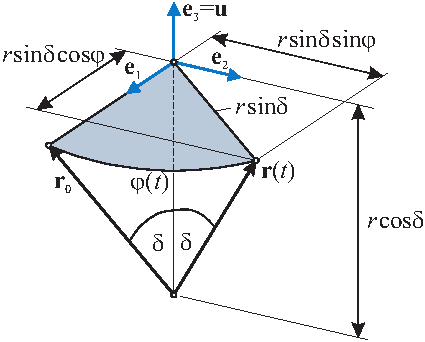
\includegraphics[width=12cm]{figures/RotationAxisAngleDerivation}
%\caption{Relations for derivation of rotation tensor and Rodrigues' formula.}
%\label{fig:theory:rotations:axisAngleDerivation}
%\end{center}
%\end{figure}
%

According to \fig{fig:theory:rotations:axisAngleDerivation}, we may split the vector $\rv$, which has the length $r = \vert \rv \vert$, into
\be 
  \rv= c_1 \ev_1 + c_2 \ev_2 + c_3 \ev_3 
\ee
with the unit vectors given as
\be
  \ev_1  =  \frac{\rv_0 - \uv(\uv^{\mathrm{T}} \rv_0)}{r \sin \delta},  \quad
  \ev_2  =  \frac{\tilde{\uv} \rv_0}{r \sin \delta}, \quad \mathrm{and} \quad 
  \ev_3  =   \uv \eqDot
\ee
The coefficients can be calculated as follows,
\be
  c_1 = r \sin \delta \cos \varphi, \quad
  c_2 = r \sin \delta \sin \varphi, \quad \mathrm{and} \quad
  c_3 = r \cos \delta
\ee
Putting everything together gives
\be 
  \rv = \cos \varphi \, \rv_0 + \sin \varphi \, \tilde{\uv} \, \rv_0 + (1 - \cos \varphi) \, \uv \, (\uv\tp \, \rv_0)
\ee
From the relation $\rv = \Rot(\uv ,\varphi) \rv_0$, we can reinterpret the \mybold{rotation tensor} $\Rot$
\be
  \Rot(\uv ,\varphi) = \cos \varphi \, \Im + \sin \varphi \, \tilde{\uv} + (1-\cos \varphi) \, \uv \, \uv\tp
\ee
%
With the additional relations
\be 
  \uv \, \uv\tp=\tilde\uv \, \tilde\uv +(\uv\tp \uv) \Im \quad \mathrm{and} \quad \uv\tp \uv = 1
\ee
we finally obtain
\be 
  \Rot(\uv ,\varphi) =  \Im + \sin \varphi \, \tilde{\uv} + (1-\cos \varphi) \,  \tilde{\uv} \, \tilde{\uv}
\ee
which is also known as the \mybold{Rodrigues formula} for rotations. 
While this formula is coordinate-free, it may be represented in any coordinate system, such as
\be 
  \LU{0}{\rv}(t)=\LU{0}{\Rot}(t) \, \LUR{0}{\rv}{0} \qquad \text{with} \qquad \LU{0}{\Rot}(t)=\Rot(\LU{0}{\uv}(t),\varphi(t))
\ee    

%+++++++++++++++++++++++++++++++++++++++++++++++++++++++++++++++++++++++++++++++
\mysubsubsubsection{Rotation vector}
%
Using the rotation vector $\vv_\mathrm{rot} = \varphi\cdot \uv$ and $\varphi = |\vv_\mathrm{rot}|$, another representation of the rotation tensor follows as
\be 
  \Rot(\uv ,\varphi) =  \Im + \frac{\sin \varphi}{\varphi} \tilde\vv_\mathrm{rot} + \frac{(1-\cos \varphi)}{\varphi^2} \,  \tilde\vv_\mathrm{rot} \, \tilde\vv_\mathrm{rot}
\ee
Note, that we inherently assume that $\varphi \in [0,\pi]$.
%
\noindent In \codeName, there are the following \mybold{functions and items related to the rotation vector} and the axis-angle representation:
\bi
  \item \texttt{NodeRigidBodyRotVecLG}: A 3D rigid body node based on rotation vector and Lie group methods; can be used for explicit integration methods, not leading to singularities when integrating with Lie-group methods
  \item \texttt{RotationVector2RotationMatrix}: computes the rotation matrix from a given rotation vector $\vv_\mathrm{rot}$
  \item \texttt{RotationMatrix2RotationVector}: computes the rotation vector $\vv_\mathrm{rot}$ from a given rotation matrix, based on a reconstruction of Euler parameters
  \item \texttt{ComputeRotationAxisFromRotationVector}: computes the rotation axis $\uv$ from the rotation vector by using $\varphi = |\vv_\mathrm{rot}|$
\ei
%
Note the following \mybold{properties of the rotation tensor}:
\bi
  \item The axis-angle representations $(\uv, \varphi)$ and $(-\uv, -\varphi)$ represent the same tensor $\Rot(\uv,\varphi)=\Rot(-\uv,-\varphi)$
  \item The rotation tensor $\Rot$ is orthogonal, i.e., $\Rot\tp \, \Rot = \Em$. 
  \item The inverse rotation tensor $\Rot^{-1} = \Rot\tp$ is represented by the identical axis-angle tuples $(\uv, -\varphi)$ and $(-\uv, \varphi)$, leading to $\rv_0=\Rot(\uv, -\varphi) \rv$.
  \item We furthermore not the identities: $\Rot(\uv, -\varphi) \equiv \Rot(-\uv, \varphi) \equiv \Rot\tp (\uv, \varphi)$
  \item The rotation axis is invariant to the rotation: $\Rot(\uv, \varphi) \uv = \uv$
  %
\ei
}

%+++++++++++++++++++++++++++++++++++++++++++++++++++++++++++++++++++++++++++++++
%+++++++++++++++++++++++++++++++++++++++++++++++++++++++++++++++++++++++++++++++
\mysubsubsection{Euler angles: Tait-Bryan angles}
%general explanation as Rx*Ry*Rz
%refer to node
%update node (refer to this section!)
%include relations with angular velocity
%see robotics / EMKL script page 33
In the following section, we discuss rotation matrices built by Tait-Bryan angles, which are consecutive $xyz$-rotations.
Note that there are many other representations of Euler angles, however, they are not implemented or used in \codeName.
The output variable \texttt{Rotation} gives Tait-Bryan angles, which is why it is important to define their properties.

%
\LatexRSTfigure{figures/theoryRotationsTaitBryanAngles}{fig:theory:rotations:TaitBryanAngles}{8cm}{240}{Definition of Tait-Bryan angles.}
%\begin{figure}[tbph]
%\begin{center}
%\includegraphics[width=12cm]{figures/theoryRotationsTaitBryanAngles}
%\caption{Definition of Tait-Bryan angles.}
%\label{fig:theory:rotations:TaitBryanAngles}
%\end{center}
%\end{figure}
%

\noindent The transformation given by Tait-Bryan angles $(\alpha,\beta,\gamma)$ follows from three successive rotations,
\be
  \LU{0}{\rv} = \LU{01}{\Rot}(\alpha) \, \LU{12}{\Rot}(\beta) \, \LU{23}{\Rot}(\gamma) \, \LU{3}{\rv} \quad
  \mathrm{and} \quad \LU{0}{\rv} = \LU{03}{\Rot}(\alpha,\beta,\gamma) \, \LU{3}{\rv}
\ee
The \mybold{Tait-Bryan rotation matrix} is thus defined as
\be
  \LU{03}{\Rot}(\alpha,\beta,\gamma) = \mr{\co\beta \,\co\gamma}{-\co\beta\,\si\gamma}{\si\beta} {\co \alpha \,\si \gamma + \si \alpha \,\si \beta \,\co \gamma}{\co \alpha \,\co\gamma-\si\alpha\,\si\beta\,\si\gamma}{-\si\alpha\,\co\beta} {\si\alpha\,\si\gamma-\co\alpha\,\si\beta\,\co\gamma}{\si\alpha\,\co\gamma+\co\alpha\,\si\beta\,\si\gamma}{\co\alpha\,\co\beta}
\ee
While not fully obvious from the latter equations, we note that there is a singularity at $|\beta| = \frac{\pi}{2}$, which causes any computations to stall whenever getting close enough to this value.

\noindent It is also possible to reconstruct Tait-Bryan angles from a given rotation matrix.
Assume, we have the rotation matrix $\LU{03}{\Rot}=(A_{ij})$.
There are two solutions for $\beta$ which follow from
\be
  \cos \beta = \pm \sqrt{1-A_{13}^2}, \quad \mathrm{and} \quad \sin \beta = A_{13}
\ee
For beta fulfilling $|\beta| \ne \frac{\pi}{2}$, we can uniquely compute $\gamma$ and $\alpha$,
\be
  \cos \gamma = \frac{A_{11}}{\cos \beta}, \quad \sin \gamma = - \frac{A_{12}}{\cos \beta}, \quad
  \cos \alpha = \frac{A_{33}}{\cos \beta}, \quad \mathrm{and} \quad \sin \alpha = - \frac{A_{23}}{\cos \beta} \eqDot
\ee
Note that improvements are possible using the $\mathrm{atan2}()$ function.
We can finally resolve non-uniqueness by restricting $\beta$ within the range $-\frac{\pi}{2} < \beta < \frac{\pi}{2}$.

\mysubsubsubsection{Tait-Bryan angles: angular velocity vector}
%
Angular velocities are essential for the formulation of equations of motion of rigid bodies, for constraints and for evaluation.
Therefore, basic relations are shown for Tait-Bryan angles, in particular the velocity transformation matrix $\Gm_{TB}$.

The angular velocity vector $\omega$ can either be computed from the basic relation $\dot \Rot = \tilde \omega \Rot$, which however involves many trigonometric terms, or from partial angular velocities, being part of the co-rotated rotation axes.
With the latter approach, we see that
\be
  \tomega_{30}=\dot{\alpha} \ev_{x0}+\dot{\beta} \ev_{y1}+\dot{\gamma} \ev_{z2} \quad \text{or} \quad 
  \tomega_{30}=\underbrace{[\ev_{x0} \quad \ev_{y1} \quad \ev_{z2}]}_{\Gm_{TB}} \vr{\dot{\alpha}}{\dot{\beta}}{\dot{\gamma}}
\ee
We can now evaluate this equation in frame $\mathcal{F}_0$ with $\tbeta=[\alpha\;\beta\;\gamma]\tp$, written as
\be 
  \LUR{0}{\tomega}{30}=\underbrace{[\LUR{0}{\ev}{x0} \quad \LUR{0}{\ev}{y1} \quad \LUR{0}{\ev}{z2}]}_{\LUR{0}{\Gm}{TB}} \vr{\dot{\alpha}}{\dot{\beta}}{\dot{\gamma}} = 
  \LUR{0}{\Gm}{TB}(\tbeta) \dot{\tbeta} \eqDot
\ee
Evaluating the consecutive rotations, we find the respective unit vectors as
\be
  \LUR{0}{\ev}{x0} = \vr{1}{0}{0}, \quad
  \LUR{0}{\ev}{y1} = \vr{0}{\text{c} \alpha}{\text{s} \alpha}, \quad \mathrm{and} \quad
  \LUR{0}{\ev}{z2} = \vr{\text{s} \beta}{-\text{s} \alpha \text{c} \beta}{\text{c} \alpha \text{c} \beta} \eqDot
\ee
which results in the relations for the (global) angular velocity vector
\be \label{eq:theory:rotations:TaitBryanG}
  \vr{\LUR{0}{\omega}{30x}}{\LUR{0}{\omega}{30y}}{\LUR{0}{\omega}{30z}} = 
  \mr{1}{0} {\text{s} \beta}
  {0}{\text{c} \alpha} {-\text{s} \alpha \text{c} \beta}
  {0}{\text{s} \alpha} {\text{c} \alpha \text{c} \beta}  
  \vr{\dot{\alpha}}{\dot{\beta}}{\dot{\gamma}} 
\ee
The matrix $\LUR{0}{\Gm}{TB}$ is used to compute partial derivatives of the angular velocity vector w.r.t.\ rotations.
However, it is also used to project torques and angular velocities into a space given by $\Gm_{TB}^\mathrm{T}$ (which is indeed not equivalent to $\Gm_{TB}^{-1}$, but gives a symmetric mass matrix -- see the equations of motion for the rigid body).

The inverse relation between $\dot \tbeta$ and $\LUR{0}{\tomega}{30}$ gives
\be \label{eq:theory:rotations:TaitBryanGinv}
  \vr{\dot{\alpha}}{\dot{\beta}}{\dot{\gamma}} = \frac{1}{\text{c} \beta} \mr{\text{c} \beta}{\text{s} \alpha \, \text{s} \beta}{-\text{c} \alpha \, \text{s} \beta}{0}{\text{c} \alpha \, \text{c} \beta}{\text{s} \alpha \text{c} \beta}{0}{-\text{s} \alpha}{\text{c} \alpha}  \vr{\LUR{0}{\omega}{30x}}{\LUR{0}{\omega}{30y}}{\LUR{0}{\omega}{30z}}
\ee
or in compact form
\be
  \dot{\tbeta} = \LURU{0}{\Gm}{TB}{-1}(\tbeta)  \LUR{0}{\tomega}{30}
\ee
We again see that for the case $\vert \beta \vert = \pi/2$ the matrix$\LUR{0}{\Gm}{TB}$ becomes singular, and \eq{eq:theory:rotations:TaitBryanGinv} cannot be resolved for $\dot{\tbeta}$!

\noindent Finally, we also provide the relations of $\tomega_{30}$ in body-fixed (local) coordinates $\mathcal{F}_3$,
which are frequently used in the implementation,
\be
  \vr{\LUR{3}{\omega}{30x}}{\LUR{3}{\omega}{30y}}{\LUR{3}{\omega}{30z}} = \mr{\text{c} \beta \, \text{c} \gamma}{\text{s} \gamma}{0}{-\text{c} \beta \, \text{s} \gamma}{\text{c} \gamma}{0}{\text{s} \beta}{0}{1} \vr{\dot{\alpha}}{\dot{\beta}}{\dot{\gamma}} \eqComma
\ee
which reads in compact form ($\LUR{3}{\Gm}{TB} = \LUR{b}{\Gm}{TB}$),
\be
  \LUR{3}{\tomega}{30} =  \LUR{3}{\Gm}{TB}(\tbeta) \dot{\tbeta}
\ee

\noindent In \codeName, there are the following \mybold{functions and items related to Tait-Bryan angles}:
\bi
  \item \texttt{NodeRigidBodyRxyz}: A 3D rigid body node based on Tait-Bryan angles
  \item \texttt{RotXYZ2RotationMatrix}: computes the rotation matrix from given Tait-Bryan angles
  \item \texttt{RotationMatrix2RotXYZ}: computes Tait-Bryan angles from a given rotation matrix
  \item \texttt{RotXYZ2G}: computes the matrix $\LU{0}{\Gm}$ relating time derivatives of Tait-Bryan angles to the (global) angular velocity vector
  \item \texttt{RotXYZ2Glocal}: computes the matrix $\LU{b}{\Gm}$ relating time derivatives of Tait-Bryan angles to the (local, body-fixed) angular velocity vector
\ei



%+++++++++++++++++++++++++++++++++++++++++++++++++++++++++++++++++++++++++++++++
%+++++++++++++++++++++++++++++++++++++++++++++++++++++++++++++++++++++++++++++++
\mysubsubsection{Euler parameters and unit quaternions}
%refer to node
%update node (refer to this section!)

As one of the most important forms of rotational parameters for multibody systems, the 4 Euler parameters are introduced.
They can be mathematically represented as unit quaternions and provide particularly simple expressions and equations of motion, albeit at the expense of an additional constraint.

The Euler parameters are defined as
\be \label{eq:theory:rotations:eulerParametersDef}
  \underline{\pv}=\vp{p_{\mathrm{s}}}{\pv}=\vp{\cos \frac \varphi 2}{\uv \, \sin \frac\varphi 2} \quad \text{bzw.} \quad \underline{\pv}=\vfour{p_{\mathrm{s}}}{p_x}{p_y}{p_z}=\vfour{\cos \frac\varphi 2}{u_x \, \sin \frac\varphi 2}{u_y \, \sin \frac\varphi 2}{u_z \, \sin \frac\varphi 2}
\ee
Here, $p_s=\cos \frac\varphi 2$ is the scalar part and $\pv = \uv \, \sin \frac\varphi 2$ is the vector part of the Euler parameters $\underline{\pv}$.
The four Euler parameters $\underline{\pv}$ are subject to the normalization condition
\be 
  \phi(\underline{\pv}) \equiv p_s^2+p_x^2+p_y^2+p_z^2-1=0 \quad \mathrm{or} \quad  p_s^2 +\pv\tp \, \pv -1 = 0 \eqDot
\ee
First, the following trigonometric transformations are introduced,
\be
  \cos \varphi = 2 \cos^2\frac{\varphi}{2} -1, \quad \sin \varphi = 2 \sin \frac \varphi 2 \cos \frac \varphi 2, \quad 1-\cos \varphi = 2 \sin^2 \frac{\varphi}{2} \eqDot
\ee
When these are substituted into the rotation tensor using \eq{eq:theory:rotations:eulerParametersDef}, it follows
\be 
  \Rot(\underline{\pv})=(2 p_{\mathrm{s}}^2-1) \, \Em + 2 p_{\mathrm{s}} \, \tilde{\pv} + 2 \, \pv \, \pv\tp \eqDot
\ee

Euler parameters can initially be expressed in the global reference frame $\mathcal{F}_0$,
\be
  \LU{0}{\underline{\pv}}=\vp{p_{\mathrm{s}}}{\LU{0}{\pv}}=\vp{\cos \frac\varphi 2}{\LU{0}{\uv} \, \sin \frac{\varphi} {2}} \eqDot
\ee
Thus, the coordinate representation of the rotation tensor is given by
\be \label{eq:theory:rotations:eulerParametersRot}
  \Rot(\LU{0}{\underline{\pv}}) = 2 \LU{0}{\mr{\ps^2+p_x^2-\frac 1 2}{p_x p_y-\ps p_z}{p_x p_z+\ps p_y} 
                                {p_x p_y+\ps p_z}{\ps^2+p_y^2-\frac 1 2}{p_y p_z-\ps p_x} 
                                {p_x p_z-\ps p_y}{p_y p_z+\ps p_x}{\ps^2+p_z^2-\frac{1}{2} }} = \LU{01}{\Rot}
\ee
Note that the axis of rotation is invariant to the rotation, $\LU{0}{\uv} = \LU{1}{\uv}$, thus $\LU{0}{\underline{\pv}} = \LU{1}{\underline{\pv}}$
Due to the ambiguity $\Rot(\underline{\pv}) = \Rot(-\underline{\pv})$, the scalar part of the Euler parameters is usually normalized, i.e., $p_s \ge 0$.

\noindent The careful reader may observe that matrix $\Rot$ in \eq{eq:theory:rotations:eulerParametersRot} is not identical to the implementation in \codeName.
This is true, because there is always an alternative formulation for the diagonal terms by adding the normalization condition times a factor.

%+++++++++++++++++++++++++++++++++++++++++++++++++++++++++++++++++++++++++++++++
\mysubsubsubsection{Quaternion operations}
%
Calculations with Euler parameters are efficiently performed through the rules of quaternion algebra.
Active perspective as vector rotation: The rotation of vector $\rv_0$ into $\rv(t)$,
\be \label{eq:theory:rotations:quaternionRotation}
  \LU{0}{\rv}(t)=\LU{0}{\Rot}(t) \, \LUR{0}{\rv}{0} \quad \text{mit} \quad \LU{0}{\Rot}(t)= \Rot(\LU{0}{\uv}(t), \varphi (t))
\ee
is formulated using the quaternion $\LU{0}{\underline{\pv}}=\underline{\pv}(\LU{0}{\uv}, \varphi)$ and its conjugate $\myoverline{\underline{\pv}}$ with the help of the double quaternion product (operator $\circ$),
\be 
  \LU{0}{\underline{\rv}}(t) = \LU{0}{\underline{\pv}}(t) \, \circ \, \LUR{0}{\underline{\rv}}{0} \, \circ \, \LU{0}{\underline{\myoverline{\pv}}}(t) \eqComma
\ee
or in short form,
\be
\vp{0}{\LU{0}{\rv}(t)}=\vp{p_{\mathrm{s}}(t)}{\LU{0}{\pv}(t)} \, \circ \, \vp{0}{\LUR{0}{\rv}{0}} \, \circ \, \vp{p_{\mathrm{s}}(t)}{-\LU{0}{\pv}(t)} \eqDot
\ee
With the multiplication rule for quaternions, the scalar part yields $0=0$ and the vector part the vector rotation \eqref{eq:theory:rotations:quaternionRotation}. 
For multiple rotations, we have
\be
  \LUR{0}{\underline{\rv}}{2}=\LUR{0}{\underline{\pv}}{2} \circ \LUR{0}{\underline{\pv}}{1} \circ \LUR{0}{\underline{\rv}}{0} \circ  \LUR{0}{\myoverline{\underline{\pv}}}{1} \circ \LUR{0}{\myoverline{\underline{\pv}}}{2} \eqDot
\ee
Given two quaternions
\be
  \underline{\av} = a_\mathrm{s} + \mathrm{i}\, a_x + \mathrm{j}\, a_y + \mathrm{k}\, a_z, \quad \mathrm{and} \quad \underline{\bv} = b_\mathrm{s} + \mathrm{i}\, b_x + \mathrm{j}\, b_y + \mathrm{k}\, b_z \eqComma
\ee
we provide two important \mybold{rules of quaternion algebra}, which is the sum,
\be
  \underline{\cv} = \underline{\av} + \underline{\bv} \quad \ra \quad 
  \vp{c_\mathrm{s}}{\cv} = \vp{a_\mathrm{s}}{\av} + \vp{b_\mathrm{s}}{\bv} = \vp{a_\mathrm{s} + b_\mathrm{s}}{\av + \bv} \eqComma
\ee
and the multiplication
\be
  \underline{\cv} = \underline{\av} \circ \underline{\bv} \neq \underline{\bv} \circ \underline{\av} \quad \ra \quad
  \vp{c_\mathrm{s}}{\cv} = \vp{a_\mathrm{s}}{\av} \circ \vp{b_\mathrm{s}}{\bv} = 
   \vp{a_\mathrm{s} b_\mathrm{s} - \av^\mathrm{T} \bv}{a_\mathrm{s}\bv + b_\mathrm{s}\av + \tilde \av \bv} \eqDot
\ee


%+++++++++++++++++++++++++++++++++++++++++++++++++++++++++++++++++++++++++++++++
\mysubsubsubsection{Angular velocity vector}
%
To derive the angular velocity from Euler parameters, there are both the possibilities of deriving the rotation matrix with respect to time and directly deriving the angular velocity from Euler parameters.

\noindent For an infinitesimal rotation $\dd \psi$, the quaternion follows
\be
  \underline{\pv}(\ev, \dd \psi) = \vp{\cos \frac{\dd \psi}{2}}{\ev \sin \frac{\dd\psi}{2}} \approx 
    \vp{1}{\ev \frac{\dd\psi}{2}}
\ee
from which we conclude that from $\underline{\pv}(\ev, \dd \psi) \, \circ \, \underline{\pv}(t) = \underline{\pv}(t) + \dd\underline{\pv}$ and thus $\dd\underline{\pv} = \vp{0}{\ev \frac{\dd\psi}{2}}$.
Dividing by $\dd t$ and with the angular velocity $\tomega_{10} = \ev \, \dot \psi$, it follows
\be
  \vp{\dot \ps}{\LLdot{0}{\pv}{}} = \frac{1}{2} \vp{0}{\tomega_{10} }  \circ \vp{\ps}{\pv}
\ee
or in short form
\be
  \LU{0}{\underline{\dot \pv}} = \frac{1}{2} \underline{\tomega}_{10}  \circ \underline{\pv}
\ee
With the quaternion product in matrix notation, it follows
\be
  \vp{\dot \ps}{\LU{0}{\dot\pv}{}} = \frac{1}{2} \mp{\ps}{-\pv^\mathrm{T}}{\pv}{\ps \Em - \tilde \pv} \vp{0}{\tomega_{10} }
\ee
or with the matrix $\underline{\Pm}$ it can be written as
\be
  \LU{0}{\underline{\dot \pv}}{} = \frac{1}{2} {\underline{\Pm}}(\pv) \underline{\tomega}_{10}    
\ee
This form can be represented in global coordinates due to ${\underline{\Pm}}^{-1} = {\underline{\Pm}}\tp$ as
\be
  \vp{0}{\LU{0}{\tomega}_{10} } = 2 \mp{\ps}{\LU{0}{\pv}^\mathrm{T}}{-\LU{0}{\pv}}{\ps \Em + \LU{0}{\tilde \pv}} \, \vp{\dot \ps}{\LLdot{0}{\pv}{}}
\ee
Thus, the velocity transformation follows to
\be
  \LUR{0}{\Gm}{EP} = \left[-2\LU{0}{\pv}, \; 2\ps \Em + 2\LU{0}{\tilde \pv}\right]
\ee
as a matrix with 3 rows and 4 columns. With $\LUR{0}{\Gm}{EP}$, the angular velocity vector can be conveniently calculated,
\be
  \LU{0}{\tomega}_{10} = \left[-2\LU{0}{\pv}, \; 2\ps \Em + 2\LU{0}{\tilde \pv}\right] \, \LU{0}{\underline{\dot \pv}}
\ee

\noindent In \codeName, there are the following \mybold{functions and items related to Euler parameters}:
\bi
  \item \texttt{NodeRigidBodyEP}: A 3D rigid body node based on Euler parameters
  \item \texttt{EulerParameters2RotationMatrix}: computes the rotation matrix from given Euler parameters
  \item \texttt{RotationMatrix2EulerParameters}: computes Euler parameters from a given rotation matrix
  \item \texttt{EulerParameters2G}: computes the matrix $\LUR{0}{\Gm}{EP}$ relating time derivatives of Euler parameters to the (global) angular velocity vector
  \item \texttt{EulerParameters2Glocal}: computes the matrix $\LUR{b}{\Gm}{EP}$ relating time derivatives of Euler parameters to the (local, body-fixed) angular velocity vector
\ei



%+++++++++++++++++++++++++++++++++++++++++++++++++++++++++++++++++++++++++++++++
%+++++++++++++++++++++++++++++++++++++++++++++++++++++++++++++++++++++++++++++++
\mysubsectionlabel{Integration Points}{sec:integrationPoints}
For several tasks, especially for finite elements and contact, different integration rules are used, which are summarized here.
The interval of all integration rules is $\in [-1,1]$, thus giving a total sum for integration weights of 2.
The points $\xi_{ip}$ and weights $w_{ip}$ for Gauss rules read:

The following table collects some typical \mybold{input parameters} for nodes, objects and markers: \vspace{-12pt}
\startGenericTable{| c | c | c | c | c |}
\rowTableFive{\mybold{type/order}}{ \mybold{point 0}}{ \mybold{point 1}}{ \mybold{point 2}}{ \mybold{point 3} }
\rowTableFive{Gauss 1}{ 0}{}{}{}
\rowTableFive{Gauss 3}{ $-\sqrt{1 / 3}$}{ $\sqrt{1 / 3}$}{}{}
\rowTableFive{Gauss 5}{ $-\sqrt{3 / 5}$}{ 0}{ $\sqrt{3 / 5}$}{}
\rowTableFive{Gauss 7}{ $-\sqrt{3 / 7 + \sqrt{120} / 35}$}{ $-\sqrt{3 / 7 - \sqrt{120} / 35}$}{ $\sqrt{3 / 7 - \sqrt{120} / 35}$}{ $\sqrt{3 / 7 + \sqrt{120} / 35}$ }
\rowTableFive{}{}{}{}{}
\rowTableFive{\mybold{type/order}}{ \mybold{weight 0}}{ \mybold{weight 1}}{ \mybold{weight 2}}{ \mybold{weight 3} }
\rowTableFive{Gauss 1}{ 2}{}{}{}
\rowTableFive{Gauss 3}{ 1}{ 1}{}{}
\rowTableFive{Gauss 5}{ $5 / 9$}{ $8 / 9$}{ $5 / 9$}{ }
\rowTableFive{Gauss 7}{ $1 / 2 - 5 / (3 \sqrt{120})$}{ $1 / 2 + 5 / (3*\sqrt{120})$}{ $1 / 2 + 5 / (3*\sqrt{120})$}{ $1 / 2 - 5 / (3*\sqrt{120})$ }
\finishTable

The points $\xi_{ip}$ and weights $w_{ip}$ for Lobatto rules read: \vspace{-12pt}
\startGenericTable{| c | c | c | c | c |}
\rowTableFive{\mybold{type/order}}{ \mybold{point 0}}{ \mybold{point 1}}{ \mybold{point 2}}{ \mybold{point 3}}
\rowTableFive{Lobatto 1}{ -1}{ 1}{}{}
\rowTableFive{Lobatto 3}{ -1}{ 0}{ 1}{}
\rowTableFive{Lobatto 5}{ -1}{ $-\sqrt{1/5}$}{ $\sqrt{1/5}$}{ 1}
\rowTableFive{}{}{}{}{}
\rowTableFive{\mybold{type/order}}{ \mybold{weight 0}}{ \mybold{weight 1}}{ \mybold{weight 2}}{ \mybold{weight 3} }
\rowTableFive{Lobatto 1}{ 1}{ 1}{}{}
\rowTableFive{Lobatto 3}{ $1/3$}{ $4/3$}{ $1/3$}{}
\rowTableFive{Lobatto 5}{ $1/6$}{ $5/6$}{ $5/6$}{ $1/6$}
\finishTable
Further integration rules can be found in the C++ code of \codeName, see file \texttt{BasicLinalg.h}.




%RST files only considered up to here
%%RSTCOMPATIBLE

%+++++++++++++++++++++++++++++++++++++++++++++++++++++++++++++++++++++++++++++++++++++++++++
\newpage
\mysubsectionlabel{Model order reduction and component mode synthesis}{sec:theory:CMS}
%terminology: eigenmode, eigenvector, eigenvalue, normal mode, static mode

This section describes the process how to create general flexible multibody system models using the floating frame of reference formulation with model order reduction (here also denoted as \hac{CMS}). The according object \texttt{ObjectFFRFreducedOrder} is described in \refSection{sec:item:ObjectFFRFreducedOrder}.

\mysubsubsection{Import of flexible bodies}
%
For flexible bodies in multibody systems, specifically for model order reduction, a standard input data (SID) has been defined in the past \cite{Schwertassek1999}.
A recent formulation for \ac{FFRF} \cite{ZwoelferGerstmayr2021} showed that significantly less information is required for the computation of the dynamics of displacement-based solid finite elements:
\bi
  \item nodal reference positions (given in \texttt{FEMinterface} member variable \texttt{nodes['Position']})
  \item stiffness matrix (given in \texttt{FEMinterface} member variable \texttt{stiffnessMatrix})
  \item mass matrix (given in \texttt{FEMinterface} member variable \texttt{massMatrix})
  \item (given in \texttt{FEMinterface} member variable \texttt{nodes['Position']})
\ei
In addition, the following data may be needed:
\bi
  \item element connectivity: needed for visualization, surface reconstruction and stress computation
  \item list of surface elements: if not computed internally in \codeName (stored in \texttt{FEMinterface} member variable \texttt{surface})
  \item information on how to obtain stresses from the set of (reduced) coordinates:  if not computed internally in \codeName (stored in \texttt{FEMinterface} member variable \texttt{postProcessingModes} for stresses at nodal positions)
\ei
This data can be generated by an appropriate interface to NGsolve:
\bi
  \item \texttt{FEMinterface.ImportMeshFromNGsolve(...)},
\ei
or imported from ABAQUS with \texttt{FEMinterface} functions
\bi
  \item \texttt{ReadMassMatrixFromAbaqus(...)}, 
  \item \texttt{ReadStiffnessMatrixFromAbaqus(...)}, 
  \item \texttt{ImportFromAbaqusInputFile(...)} )
\ei
and similar functionality exists for ANSYS.
Importing data may be time consuming, which is why all FEMinterface data, including computed modes, can be saved and loaded via
\texttt{SaveToFile} and \texttt{LoadFromFile}. 

It is assumed that there exists an underlying solid finite element mesh, given by e.g., tetrahedral or hexahedral finite elements. However, this mesh is not needed for computations. If the surface or any part of the flexible body shall be visualized, surface elements (triangles or quads) need to be provided with indices of the mesh nodes. The computation of surface elements is done by \texttt{FEMinterface} function \texttt{ VolumeToSurfaceElements}, making use of solid finite elements stored in \texttt{FEMinterface.elements}.

A major advantage of the \texttt{FEMinterface} data is that it is widely independent of underlying finite element technologies, specifically finite element order, reduced integration, etc., however, stress or strain can not be computed as well.
A conventional way is to store computed body deformations and perform post processing in the original finite element code, which gives highest quality of stress, strain, and other quantities.
A second way is, due to linearity of the small deformation assumptions, to use post-processing modes, such as modes to represent stress components. 
Post processing modes may be defined in the \texttt{FEMinterface} member \texttt{postProcessingModes}, which is a dictionary containing the modes stored in columns of the \texttt{matrix}, cyclic for every (stress / strain) component and for all modes, and an extra field \texttt{outputVariableType} which denotes the type of modes.
The post processing modes may be directly computed in NGsolve with \texttt{ComputePostProcessingModesNGsolve}, using efficient and accurate internal functionality, or calculated with a much slower and very basic Python function \texttt{ComputePostProcessingModes}, which can compute simplified stresses or strains for 4-noded tetrahedral elements. 


\mysubsubsection{Eigenmodes}
This section will describe the computation of eigenmodes using FEMinterface.

The \texttt{FEMinterface} in the module \texttt{FEM} has various functionality to import finite element meshes from finite element software.
We create a \texttt{FEMinterface} by means of
\bi
  \item[] \texttt{fem = FEMinterface()}
\ei
which allows us to use the variable \texttt{fem} from now.

Meshes can be imported from NETGEN/NGsolve (\refSection{sec:FEM:FEMinterface:ImportMeshFromNGsolve}), Abaqus (see \refSection{sec:FEM:FEMinterface:ImportFromAbaqusInputFile} and other sections related to ABAQUS), ANSYS (see \refSection{sec:FEM:FEMinterface:ReadElementsFromAnsys} and other sections related to ANSYS).
The import procedure, which can also be done manually, needs to include \texttt{massMatrix} $\Mm$ and \texttt{stiffnessMatrix} $\Km$ from any finite element model.
Note that many functions are based on the requirement that nodes are 3D displacement-based nodes, without rotation or other coordinates.

For any functionality with \texttt{ObjectFFRFreducedOrder} and for the computation of Hurty-Craig-Bampton modes as described in the next section, \texttt{nodes}
are required.
Finally, \texttt{elements} need to be included for visualization, and a surface needs to be reconstructed from the element connectivity, which is available for tetrahedral and hexahedral elements for most import functions.

%++++++++++++++++++++++++
\begin{figure}[tbph]
  \begin{center}
  \includegraphics[width=10cm]{figures/modesHinge/HCBhingeMesh.jpg}
  \end{center}
  \caption{Test model and mesh for hinge created with Netgen (linear tetrahedral elements).}
  \label{fig_hingePartMesh}
\end{figure}
%++++++++++++++++++++++++
As an example, we consider a part denoted as 'hinge' in the following, see \fig{fig_hingePartMesh}. The test example can be found in \texttt{Examples/NGsolveCMStutorial.py} with lots of additional features.

After import of mass and stiffness matrix, eigenmodes and eigenfrequencies can be computed using \texttt{fem.ComputeEigenFrequencies(...)}, 
which computes the quantities \texttt{fem.modeBasis} and \texttt{fem.eigenValues}.
The eigenvalues in Hz can be retrieved also with the function \texttt{fem.GetEigenFrequenciesHz()}.
The function \texttt{fem.ComputeEigenFrequencies(...)} is available for dense and sparse matrices, and uses \texttt{scipy.linalg} to compute eigenvalues of the linear, undamped mechanical system
\be \label{theory:eigenmodes:EOM}
  \Mm \ddot \qv(t) + \Km \qv(t) = \fv(t) \eqDot
\ee
Here, the total number of coordinates of the system is $n$, 
thus having the vector of system coordinates $\qv \in \Rcal^n$, 
vector of applied forces $\fv \in \Rcal^n$, 
mass matrix $\Mm \in \Rcal^{n \times n}$ and stiffness matrix $\Km \in \Rcal^{n \times n}$. 
If we are interested in free vibrations of the system, without any boundary conditions or interconnections to other bodies, \eq{theory:eigenmodes:EOM} can be converted to a generalized eigenvalue problem. Using the approach 
$\qv(t) = \vv \mathrm{e}^{\mathrm{i} \omega t}$ in \eq{theory:eigenmodes:EOM}, and thus $\ddot \qv(t) = -\omega^2 \qv(t)$, we obtain
\be \label{theory:eigenmodes:harmonicEquation}
    \left[ \left(-\omega^2 \Mm + \Km \right) \vv \right] \mathrm{e}^{i\omega t} = \Null \eqDot
\ee
Assuming that \eq{theory:eigenmodes:harmonicEquation} is valid for all times, the \mybold{generalized eigenvalue problem} follows that
\be \label{theory:eigenmodes:GEP}
  \left(-\omega^2 \Mm + \Km \right) \vv = \Null \eqComma
\ee
which can be rewritten as
\be \label{theory:eigenmodes:GEP2}
  \det \left(-\omega^2 \Mm + \Km \right) = 0 \eqComma
\ee
and which defines the eigenvalues $\omega_i^2$ of the linear system, where $i \in \{0, \ldots, n-1\}$. Note that in this case, the eigenvalues are the squared eigenfrequencies (in rad/s).
We can use eigenvalue algorithms to compute the eigenvalues $\omega_i^2$ and according eigenvectors $\vv_i$ from Python.
The function \texttt{fem.ComputeEigenmodes(...)} uses \texttt{eigh(...)} from \texttt{scipy.linalg} in the dense matrix mode, 
and in the sparse mode \texttt{eigsh(...)} from \texttt{scipy.sparse.linalg}, the latter being restricted to pure symmetric matrices.
Using special shift-inverted techniques in \texttt{eigsh(...)}, it performs much better than standard settings. However, you may tune your specific eigenvalue problem by modifying the solver procedure (just copy that function and adjust to your needs).
As an output, we obtain the smallest \texttt{nModes} eigenvectors (=eigenmodes)\footnote{Eigenvectors are the result of the eigenvalue algorithm, such as the QR algorithm. The mechanical interpretation of eigenvectors are eigenmodes, that can be visualized as shown in the figures of this section.} of the system.
Here, we will also use synonymously the terms `eigenmodes' and `normal modes', which result from an eigenvalue/eigenvector computation using certain (or even no) boundary conditions.
%++++++++++++++++++++++++
\begin{figure}[tbph]
  \begin{center}
  \includegraphics[width=4cm]{figures/modesHinge/freeFreeModeStress1}
  \includegraphics[width=4cm]{figures/modesHinge/freeFreeModeStress2}
  \includegraphics[width=4cm]{figures/modesHinge/freeFreeModeStress3}
  \includegraphics[width=4cm]{figures/modesHinge/freeFreeModeStress4}\\
  \includegraphics[width=4cm]{figures/modesHinge/freeFreeModeStress5}
  \includegraphics[width=4cm]{figures/modesHinge/freeFreeModeStress6}
  \includegraphics[width=4cm]{figures/modesHinge/freeFreeModeStress7}
  \includegraphics[width=4cm]{figures/modesHinge/freeFreeModeStress8}
  \end{center}
  \caption{Lowest 8 free-free modes for hinge finite element model, contour plot for $xx$-stress component.}
  \label{fig_hingePartFreeFreeModes}
\end{figure}
%++++++++++++++++++++++++

Clearly, if there are no supports included in the stiffness matrix, the resulting eigenmodes will contain 6 rigid body modes and we will also call this case for the computation of eigenmodes the `free-free' case, in analogy to a simply supported beam.
This rigid body modes, which are usually not needed (=unwanted) in the succeeding computation, can be excluded with an according option in \vspace{6pt}\\
\texttt{fem.ComputeEigenFrequencies(excludeRigidBodyModes = ...)}
\vspace{12pt}\\
For our test example, 8 eigenmodes are shown in \fig{fig_hingePartFreeFreeModes}, where the 6 rigid body modes have been excluded (so in total, 14 eigenvectors were computed).
%free free modes (coarse mesh, nNodes= 1216):
%freq(Hz)=[ 671.59137506  707.17488417 1298.50905491 1929.97563131 1971.76505866
%3141.47119938 3595.34508711 4317.51987533]
The 8 eigenfrequencies for the chosen coarse mesh with mesh size $h=0.01$ and 1216 nodes result as 
\be
  f_{0..7} = [ 671.59, 707.17, 1298.50, 1929.97, 1971.76, 3141.47, 3595.34, 4317.51] Hz
\ee
Note, that a computation with a finer mesh, using mesh size $h=0.002$ and 100224 nodes, leads to significantly different eigenfrequencies, starting with $f_0=371.50\,$Hz. This shows that quadratic finite elements would be more appropriate for this case.

After the computation of modes, it is always a good idea to visualize and/or animate these modes. We can do this, using the function \texttt{AnimateModes(...)} available in \texttt{exudyn.interactive}, which allows us to inspect and animate modes and to create animations for these modes, see the mentioned example.

Clearly, the free-free modes in \fig{fig_hingePartFreeFreeModes} are not well suited for the modeling of the deformations within the hinge, if the bolt and the bushing shall be fixed to ground or to another part. 
%TO BE DONE:
%We investigate this by adding a simple revolute joint to the bolt.
Therefore, we can use modes based on ideas of Hurty \cite{Hurty1965} and Craig-Bampton \cite{CraigBampton1968}, as shown in the following.


%+++++++++++++++++++++++++++++++++++++++++++++++++++++++++++++++++++++++++++++++++++++++++++++++++++++++++++++++++++++++
%+++++++++++++++++++++++++++++++++++++++++++++++++++++++++++++++++++++++++++++++++++++++++++++++++++++++++++++++++++++++
%+++++++++++++++++++++++++++++++++++++++++++++++++++++++++++++++++++++++++++++++++++++++++++++++++++++++++++++++++++++++
\mysubsubsectionlabel{Hurty-Craig-Bampton modes}{sec:hurty-craig-bampton-modes}
This section will describe the computation of static and eigen (normal) modes using FEMinterface.
The theory is based on Hurty \cite{Hurty1965} and Craig-Bampton \cite{CraigBampton1968}, but often only attributed to Craig-Bampton.
Furthermore, boundaries are also called interfaces\footnote{Here, and in the description of various Python functions, we will use boundary and interface often synonymously, as flexible bodies can be either connected to ground in the sense of a classical 'support-type' boundary condition, or they can represent the boundary of the flexible body as an interface to joints (via markers).}, as they either represent surface sections of our finite element model which are connected to the ground or they represent interfaces to joints and are connected to other bodies.

The computation of so-called static and normal modes follows a simple concept based on finite element mass and stiffness matrices.
The final goal of the computation of modes is to approximate the solution $\qv \in \Rcal^n$ 
by means of a reduction basis $\tPsi \in \Rcal^{n \times m}$ 
and a reduced set of coordinates $\pv \in \Rcal^m$, for which we assume $m \ll n$.

In order to include boundary/interface effects, we separate our nodes and the nodal coordinates into 
\bi
  \item[] a) boundary nodes $\qv_b \in \Rcal^{n_b}$ and
  \item[] b) internal or inner nodes $\qv_i \in \Rcal^{n_i}$.
\ei
We assume that internal nodes are not exposed to boundary/interface conditions or to forces.

Therefore, we may rewrite \eq{theory:eigenmodes:EOM} as follows
\be \label{eq_GuyanIrons}
  \mp{\Mm_{bb}}{\Mm_{bi}}{\Mm_{ib}}{\Mm_{ii}} \vp{\ddot{\qv}_b}{\ddot{\qv}_i} + \mp{\Km_{bb}}{\Km_{bi}}{\Km_{ib}}{\Km_{ii}} \vp{\qv_b}{\qv_i} =   \vp{\fv_b}{\Null}
\ee
or, equivalently,
\bea
  \Mm_{bb} \ddot{\qv}_b + \Mm_{bi} \ddot{\qv}_i +\Km_{bb}  {\qv}_b + \Km_{bi}  {\qv}_i  = {\fv}_b \label{eq_Guyan_bb}\\
  \Mm_{ib} \ddot{\qv}_b + \Mm_{ii} \ddot{\qv}_i +\Km_{ib}  {\qv}_b + \Km_{ii}  {\qv}_i  = \Null \eqDot \label{eq_Guyan_ii}
\eea
A pure static condensation follows from \eq{eq_Guyan_ii} with the assumption that inertia terms are neglected,
leading to the static result for internal nodes,
\be 
  {\qv}_{i,stat}=-\Km_{ii}^{-1} \Km_{ib} {\qv}_{b} \eqDot 
\ee
A pure static condensation, also denoted as Guyan-Irons method, keeps boundary coordinates but removes all internal modes, using the approximation
\be
  \label{eq_guans_red}
  \vp{\qv_b}{\qv_i} \approx \vp{\Im}{-\Km_{ii}^{-1} \Km_{ib}}  \qv_b = \tPsi^{GI} \qv_b \eqComma
\ee
which leads to no approximations ('exact') results for the static case, but poor performance in highly dynamic problems.

Significant improvement result from the Hurty-Craig-Bampton method, which adds eigenmodes of the internal coordinates (internal nodes).
We assume that $\tPsi_{ii}$ is the matrix of eigenvectors as a solution to the eigenvalue problem
\be \label{theory:eigenmodes:GEPii}
  \left(-\omega^2 \Mm_{ii} + \Km_{ii} \right) \vv = \Null \eqComma
\ee
Hereafter, we will only keep the lowest (or other appropriate) $m$ eigenmodes in a reduced eigenmode matrix,
\be
  \tPsi^{(red)}_{ii} = \left[\tPsi_{ii,0}, \ldots, \tPsi_{ii,m-1} \right]
\ee
Combining these `fixed-fixed' eigenvectors with the Guyan-Irons reduction \eqref{eq_guans_red}, we obtain the 
Hurty-Craig-Bampton modes as
\be
  \vp{\qv_b}{\qv_i} \approx \vp{\Im}{-\Km_{ii}^{-1} \Km_{ib}}  \qv_b  +  \vp{\Null}{\tPsi_{r,i}}  \pv_{r} \eqComma
\ee
or in matrix form
\be \label{theory:eigenmodes:HCB}
  \vp{\qv_b}{\qv_i} \approx \mp{\Im}{\Null}{-\Km_{ii}^{-1} \Km_{ib}}{\tPsi_{r,i}}   \vp{\qv_b}{\pv_r} = \tPsi^{HCB} \pv^{HCB} \eqDot
\ee
The disadvantage of \eq{theory:eigenmodes:HCB} is evident by the fact that there may be a large number of boundary/interface nodes, leading to a huge number of static modes (100s or 1000s) and thus making the model reduction inefficient. Therefore, we can switch to other interfaces, as described in the following.

\mysubsubsubsection{Definition of RBE2 / RBE3 interfaces}
A powerful extension, which is available in many finite element as well as flexible multibody codes, is the definition of special boundary/interface conditions, based on pure rigid body motion.
The so-called RBE2 boundaries are defined such that they are firmly connected to a rigid frame, thus the boundary or interface can only undergo rigid body motion.
The advantage of this procedure is that, in comparison to \eq{theory:eigenmodes:HCB}, the number of boundary/interface modes is given by 6 {\it rigid body} modes, which allow simple integration into standard joints of multibody systems, e.g., the \texttt{GenericJoint}.
The disadvantage is that such modes usually lead to artificial stiffening and stresses close to the boundary.

For so-called RBE3 boundaries, the kinematics is significantly different. The displacement of RBE3 boundaries is the (weighted) average displacement of all boundary nodes. The resulting forces at the RBE3 boundary are equally distributed, again using node-weighting.
The (linearized) rotation of RBE3 boundaries is computed as the weighted displacements of the boundaries and including the distance to the rotation axes. 
Forces due to torques at RBE3 boundaries are computed according to the weighting, again considering the distance to the rotation axes, see the according formulas later on. The computation of RBE3 boundaries widely follows the formulation of the \texttt{MarkerSuperElementRigid}, see \refSection{sec:item:MarkerSuperElementRigid}.

\mysubsubsubsection{Computation of Hurty-Craig-Bampton modes with RBE2 interfaces}
In the following section, we show the procedure for the computation of static modes for the RBE2 rigid-body interfaces.
Note that eigenmodes directly follow from matrices $\Mm_{ii}$ and $\Km_{ii}$ as described in \refSection{sec:hurty-craig-bampton-modes}.
The implementation is given in \texttt{fem.ComputeHurtyCraigBamptonModes(...)}, see \refSection{sec:FEM:FEMinterface:ComputeHurtyCraigBamptonModes}.

First, we use the index $j$ here as a node index, having the clear correspondence to the coordinate index $i$, that node $j$ has coordinates 
$[3\cdot j,\; 3\cdot j+1,\; 3\cdot j+2]$.
Furthermore, nodes are split into boundary and internal nodes, which then leads to according internal and boundary coordinates.
We shall note that this sorting is never done in the finite element model or matrices, but just some indexing (referencing) lists are generated and used throughout, using valuable features of \texttt{numpy.linalg} and \texttt{scipy.sparse}.

For a certain boundary node set $B=[j_0, \; j_1, \; j_2, \; ...] \in \Ncal^{n_b}$ with certain $n_b$ node indices $j_0, ...$, we define one boundary set. The following transformations need to be performed for every set of boundary node lists. We also assume that weighting of all boundary nodes is equal, which may not be appropriate in all cases.

If we assume that there may only occur rigid body translation and rotation for the whole boundary node set, which is according to the idea of so-called RBE2 boundary conditions, it follows that the translation of all boundary nodes is given by
\be
  %\Tm_t = \left[ \Im \; \Im \; \ldots \; \Im \right]\tp \in \Rcal^{3 n_b \times 3}
  \Tm_t = \vr{ \Im }{ \vdots}{ \Im} \in \Rcal^{3 n_b \times 3}
\ee
with $\Im \in \Rcal^{3\times 3}$ identity matrices. 
The nodal translation coordinates on boundary $B$ are denoted as $\qv_{B,t} \in \Rcal^3$. The translation of the boundary/interface is mapped to the boundary coordinates as follows (assuming only one boundary $B$),
\be
  \qv_{b,t} = \Tm_t \, \qv_{B,t}
\ee
The nodal rotation coordinates on boundary $B$ are denoted as $\qv_{B,r} \in \Rcal^3$. The rotation of the boundary/interface is mapped to the boundary coordinates as follows (assuming only one boundary $B$),
\be
  \qv_{b,r} = \Tm_r \, \qv_{B,r}
\ee
The computation of matrix $\Tm_r$ is more involved. It is based on nodal (reference) position vectors $\rv^{(0)}_j$, $j \in B$, 
the midpoint of all boundary nodes, 
\be
  \rv^{(m)} = \frac{1}{n_b} \sum_{j=0}^{n_b-1} \rv^{(0)}_j
\ee
and the position relative to the midpoint, denoted as 
\be
  \rv_j = \rv^{(0)}_j - \rv^{(m)} \eqDot
\ee
Note that the coordinate system refers to the system used in the underlying finite element mesh.
The transformation for rotation follows from 
\be
  %in old version, j should have been 0, 1, 2, ...
  %\Tm_r  = \left[ \widetilde \tOmega_x \rv_{j_0} \;\; \widetilde \tOmega_y \rv_{j_0} \;\; \widetilde \tOmega_z \rv_{j_0} \;\;
                  %\widetilde \tOmega_x \rv_{j_1} \;\; \widetilde \tOmega_y \rv_{j_1} \;\; \widetilde \tOmega_z \rv_{j_1}
                  %\ldots \right]\tp \in \Rcal^{3 n_b \times 3}
  \Tm_r = \vr{ \tilde \rv_0 }{ \vdots}{ \tilde \rv_{n_b-1}} \in \Rcal^{3 n_b \times 3} \eqDot
\ee
%with the special tensors, representing rotation about (x,y,z)-axes,
%\be
  %\widetilde\tOmega_x = \mr{0}{0}{0} {0}{0}{-1} {0}{1}{0}, \quad
  %\widetilde\tOmega_y = \mr{0}{0}{1} {0}{0}{0} {-1}{0}{0}, \quad
  %\widetilde\tOmega_z = \mr{0}{-1}{0} {1}{0}{0} {0}{0}{0} \eqDot
%\ee
%
The total nodal coordinates at the boundary, representing translations and rotations, follow as
\be
  \qv_{B} = \vp{\qv_{B,t}}{\qv_{B,r}} \eqComma
\ee
and the transformation matrix for the translation and rotation simply reads
\be
  \Tm = [\Tm_t \;\; \Tm_r] \in \Rcal^{3n_b \times 6} \eqComma
\ee
which provides the total mapping of boundary rigid body motion
\be
  \qv_{b} = \Tm \, \qv_{B} \eqComma
\ee 
which is the sum of translation and rotation.

As an example, having the boundary nodes sorted for two boundary node set $B_0$ and $B_1$, we obtain the following transformation for the Hurty-Craig-Bampton method with only 6 modes per boundary node set,
\be \label{theory:eigenmodes:HCBRBE2}
  %\vp{\qv_b}{\qv_i} \approx \mp{ \Im \mp{\Tm_0}{}{}{\Tm_1}}{\Null}{-\Km_{ii}^{-1} \Km_{ib}\vp{\Tm_0}{\Tm_1}}{\tPsi_{r,i}}   
  %\vr{\qv_{B_0}}{\qv_{B_1}}{\pv_r} \eqDot
  \vp{\qv_b}{\qv_i} \approx \mr{ \Tm_0}{\Null}{\Null} {\Null}{\Tm_1}{\Null} 
                            {-\Km_{ii}^{-1} \Km_{ib}\vp{\Tm_0}{\Null} }{-\Km_{ii}^{-1} \Km_{ib}\vp{\Null}{\Tm_1} }{\tPsi_{r,i}}   
  \vr{\qv_{B_0}}{\qv_{B_1}}{\pv_r} \eqDot
\ee
with the new boundary node vector $\qv_b = [\qv_{B_0}\tp \;\; \qv_{B_1}\tp]\tp$.

\noindent \mybold{Notes}:
\bi
  \item The inverse $\Km_{ii}^{-1} $ is not computed, but this matrix is LU-factorized using sparse techniques.
  \item The factorization only needs to be applied to six vectors for every relevant boundary node set.
  \item One set of boundary nodes can be omitted from the final static modes in \eq{theory:eigenmodes:HCBRBE2}, because keeping all boundary modes, would introduce six rigid body motions to our mode basis, what is usually not wanted nor needed.
\ei

Using again the examples given in \fig{fig_hingePartMesh}, we now obtain a set of modified modes using the function \texttt{fem.ComputeHurtyCraigBamptonModes(...)}.
\fig{fig_hingePartStaticModesA} shows the first 6 rigid body modes. Note that these modes are automatically removed in the function \texttt{fem.ComputeHurtyCraigBamptonModes(...)} with default settings.
\fig{fig_hingePartStaticModesB} shows the second set of 6 rigid body modes. 
Finally, 8 eigenmodes have been computed for the fixed-fixed case (where all boundary/interfaces nodes are fixed),
see \fig{fig_hingePartFixedFixedModes}. 
The eigenfrequencies for this case now are significantly higher than in the free-free case, reading
\be
  f_{0..7} = [1277.35, 1469.86, 3336.91, 3584.28, ...]
\ee
%Hurty-Craig-Bampton modes (coarse mesh, nNodes= 1216):
 %freq(Hz)=[1277.35052832 1469.86514681 3336.91168906 3584.28464361 5079.65220372
 %6035.58805197 6049.99829894 6568.47108075]
%++++++++++++++++++++++++
\begin{figure}[tbph]
  \begin{center}
  \includegraphics[width=5cm]{figures/modesHinge/HCBmodesHingeStaticAx}
  \includegraphics[width=5cm]{figures/modesHinge/HCBmodesHingeStaticAy}
  \includegraphics[width=5cm]{figures/modesHinge/HCBmodesHingeStaticAz}\\
  \includegraphics[width=5cm]{figures/modesHinge/HCBmodesHingeStaticArotX}
  \includegraphics[width=5cm]{figures/modesHinge/HCBmodesHingeStaticArotY}
  \includegraphics[width=5cm]{figures/modesHinge/HCBmodesHingeStaticArotZ}
  \end{center}
  \caption{Static modes for bolt rigid body interface, using Hurty-Craig-Bampton method; top three images show (x,y,z)-translation modes, bottom three images show (x,y,z)-rotation modes; contour color represents norm of displacements.}
  \label{fig_hingePartStaticModesA}
\end{figure}
%++++++++++++++++++++++++

%++++++++++++++++++++++++
\begin{figure}[tbph]
  \begin{center}
  \includegraphics[width=5cm]{figures/modesHinge/HCBmodesHingeStaticBx}
  \includegraphics[width=5cm]{figures/modesHinge/HCBmodesHingeStaticBy}
  \includegraphics[width=5cm]{figures/modesHinge/HCBmodesHingeStaticBz}\\
  \includegraphics[width=5cm]{figures/modesHinge/HCBmodesHingeStaticBrotX}
  \includegraphics[width=5cm]{figures/modesHinge/HCBmodesHingeStaticBrotY}
  \includegraphics[width=5cm]{figures/modesHinge/HCBmodesHingeStaticBrotZ}
  \end{center}
  \caption{Static modes for bushing rigid body interface, using Hurty-Craig-Bampton method; top three images show (x,y,z)-translation modes, bottom three images show (x,y,z)-rotation modes; contour color represents norm of displacements.}
  \label{fig_hingePartStaticModesB}
\end{figure}
%++++++++++++++++++++++++

%++++++++++++++++++++++++
\begin{figure}[tbph]
  \begin{center}
  \includegraphics[width=4cm]{figures/modesHinge/HCBmodesHingeEigenmode0}
  \includegraphics[width=4cm]{figures/modesHinge/HCBmodesHingeEigenmode1}
  \includegraphics[width=4cm]{figures/modesHinge/HCBmodesHingeEigenmode2}
  \includegraphics[width=4cm]{figures/modesHinge/HCBmodesHingeEigenmode3}\\
  \includegraphics[width=4cm]{figures/modesHinge/HCBmodesHingeEigenmode4}
  \includegraphics[width=4cm]{figures/modesHinge/HCBmodesHingeEigenmode5}
  \includegraphics[width=4cm]{figures/modesHinge/HCBmodesHingeEigenmode6}
  \includegraphics[width=4cm]{figures/modesHinge/HCBmodesHingeEigenmode7}
  \end{center}
  \caption{Eigenmodes for fixed-fixed case, resulting from Hurty-Craig-Bampton method; contour color represents norm of displacements.}
  \label{fig_hingePartFixedFixedModes}
\end{figure}
%++++++++++++++++++++++++


%+++++++++++++++++++++++++++++++++++++++++++++++++++++++++++++++++++++++++++++++++++++++
%+++++++++++++++++++++++++++++++++++++++++++++++++++++++++++++++++++++++++++++++++++++++
%synchronize this section with the paper!
%\mysubsubsubsection{Computation of Hurty-Craig-Bampton modes with RBE3 interfaces}
%In the following section, we show the procedure for the computation of static and eigenmodes for the RBE3 rigid-body interfaces.
%The implementation is given in \texttt{fem.ComputeHurtyCraigBamptonModes(...)}, see \refSection{sec:FEM:FEMinterface:ComputeHurtyCraigBamptonModes}.
%
%It shall be noted that there are slightly different versions of RBE3 modes, as there are several possibilities to define average displacements and rotations,
%and there are several ways to define the eigen-problem for eigenmodes.
%Here, we chose the following way to compute eigenmodes:
%\bi
  %\item at every boundary, which may not contain overlapping nodes with other boundaries, the weighted average displacement and the weighted average rotation is fixed by imposing 6 constraints per boundary;
  %\item for the computation of static modes, a single DOF at the rigid boundaries is prescribed with an average unit displacement or unit rotation.
  %\item for the computation of eigenmodes, all weighted displacements/rotations are fixed and eigenmodes are computed for lowest eigenfrequencies.
%\ei
%%
%The stiffness matrix, sorted for boundary and internal nodal coordinates reads, compare \eq{eq_GuyanIrons},
%\be
  %\Km = \mp{\Km_{bb}}{\Km_{bi}}{\Km_{ib}}{\Km_{ii}}
%\ee
%
%\noindent
%For every boundary $B \in [B0, B1, \ldots ]$ of $n_B$ boundaries, we defined linear constraints, using the same boundary node definitions as for RBE2 boundaries.
%The three linear constraints for average displacements are given for boundary nodes $j$ with displacement vectors $\qv_{b,j}$ and nodal weights per boundary $w_{B,j}$\footnote{note that the sum of all weights follows as $\sum_j w_{B,j}=1$.}, 
%\be
  %\cv_{b,t}(\qv_b) = \Cm_{b,t} \qv_b = \sum_{j=0}^{n_B-1} w_{B,j} \qv_{B,j} = \uv_B
%\ee
%which implicitly defines $\Cm_{b,t} \in \Rcal^{3 n_b \times 3}$, while $\Cm_{i,t} = \Null \in \Rcal^{3 n_i \times 3}$.
%The prescribed displacement $\uv_B$ is zero, except that this boundary mode is currently computed.
%
%For rotations, the nodal (reference) position vectors $\rv^{(0)}_j$, $j \in B$ and
%the midpoint of all boundary nodes, 
%\be
  %\rv^{(m)} = \frac{1}{n_b} \sum_{j=0}^{n_B-1} w_{B,j} \rv^{(0)}_j \eqComma
%\ee
%are again used to define positions relative to the midpoint $\rv^{(m)}$, 
%\be
  %\rv_j = \rv^{(0)}_j - \rv^{(m)} \eqDot
%\ee
%Note that the coordinate system refers to the system used in the underlying finite element mesh.
%Similar as in the \texttt{MarkerSuperElementRigid}, see \refSection{sec:item:MarkerSuperElementRigid}, 
%we define a total weighting for all nodal reference positions relative to the boundary's midpoint as
%\be
    %\Wm = -\sum_j  w_{B,j} \tilde \rv_j \tilde \rv_j \eqComma
%\ee
%which follows from the analogy of an inertia tensor with mass distributed equally at the boundary.
%
%The three linear constraints for average rotations follow as
%\be
  %\cv_{b,r}(\qv_b) = \Cm_{b,r} \qv_b = \sum_{j=0}^{n_B-1} w_{B,j} \tilde \rv_{B,j} \qv_{B,j}  = \ttheta_B
%\ee
%which implicitly defines $\Cm_{b,r} \in \Rcal^{3 n_b \times 3}$.
%Here, $\ttheta_B$ is a weighting matrix similar to the \texttt{MarkerSuperElementRigid},
%\be
  %\ttheta_B = \sum_{j=0}^{n_B-1} -w_{B,j} \tilde \rv_{B,j} \tilde \rv_{B,j}
%\ee
%Similarly as for translations, the prescribed rotation $\ttheta_B$ is zero, except that this boundary mode is currently computed.
%Finally, we combine translation and rotation part as 
%\be
  %\Cm_{b} = \vp{\Cm_{b,t}}{\Cm_{b,r}} \eqComma
%\ee
%and set $\Cm_{i} = \Null \in \Rcal^{3 n_i \times 6}$.
%In order to compute boundary modes, the linear system of equations reads
%\be \label{eq:theory:HCB:RBE3linearEq}
  %\mr{\Km_{bb}}{\Km_{bi}}{\Cm_{b}\tp} {\Km_{ib}}{\Km_{ii}}{\Cm_{i}\tp} {\Cm_{b}}{\Cm_{i}}{\Null} \vr{\qv_b}{\qv_i}{\tlambda} = \vr{\Null}{\Null}{\tdelta} \eqDot
%\ee
%Here, $\tlambda$ represents Lagrange multipliers which represent the boundary forces and torques at the according boundaries due to unit displacements or rotations, given by the vector $\tdelta$.
%In order to compute the $k^\mathrm{th}$ boundary mode as $\vp{\qv_b^k}{\qv_i^k}$, we set the $k^\mathrm{th}$ component of $\tdelta$ to
%\be
  %\tdelta_k = 1 \eqComma
%\ee
%while all other components of $\tdelta$ are $0$ and solve \eq{eq:theory:HCB:RBE3linearEq}. This way allows to compute all static modes using a single factorization in \eq{eq:theory:HCB:RBE3linearEq} to compute all modes for all boundaries.
%
%The computation of eigenmodes require to apply all constraints to the stiffness and mass matrices, which is done by means of projection of the linear equations of motion into the null space of the constraints.
%We compute the singular value decomposition for every constraint matrix $\Cm_{b}$,
%\be
  %[\Um, \sv, \Vm] = \mathrm{SVD}(\Cm_{b}), \eqComma
%\ee
%where $\Um$ is a unitary matrix with left singular vectors as columns, $\sv$ stores singular values in the diagonal, and $\Vm$ is a 
%unitary matrix with right singular vectors as rows.
%The null space of the constraint matrix $\Cm_{b}$ is spanned by $\Vm_N \in \Rcal^{(3 n_b-6) \times 3 n_b}$, which results from $\Vm$ when removing the first 6 rows. 
%Combining the null space matrix with a unit matrix for the internal nodes, $\Im_{ii} \in \Rcal^{n_i \times n_i}$,
%the projection matrix results as
%\be
  %\Vm_P = \mp{\Vm_N}{}{}{\Im_{ii}}
%\ee
%Using the projected stiffness and mass matrices,
%\be
  %\Mm_P = \Vm_P \mp{\Mm_{bb}}{\Mm_{bi}}{\Mm_{ib}}{\Mm_{ii}} \Vm_P\tp \quad \mathrm{and} \quad
  %\Km_P = \Vm_P \mp{\Km_{bb}}{\Km_{bi}}{\Km_{ib}}{\Km_{ii}} \Vm_P\tp 
%\eqComma
%\ee
%the eigenvalue problem for the constrained system of \eq{eq:theory:HCB:RBE3linearEq} is given by
%\be \label{eq:theory:HCB:RBE3eigen}
  %\Mm_P \ddot{\qv}_P + \Km_P \qv_P = \Null \eqDot
%\ee
%The eigen analysis of \eq{eq:theory:HCB:RBE3eigen} results in the eigenvector matrix $\tPsi_P \in \Rcal^{(n-6) \times m}$, containing a set of $m$ eigenvectors.
%The final eigenvectors $\tPsi \in \Rcal^{n \times m}$ are computed by means of projection onto the original boundary nodes, using
%\be
  %\tPsi = \Vm_P\tp \tPsi_P \eqDot
%\ee
%Note that for efficiency reasons operations such as in \eq{eq:theory:HCB:RBE3eigen} are only performed for boundary nodes, but not for internal nodes.
%Furthermore, sparse matrices are used whenever matrices are large and not fully populated.
%


%+++++++++++++++++++++++++++++++++++++++++++++++++++++++++++++++++++++++++++++++++++++++
\mysubsubsectionlabel{Interfaces and boundaries}{sec:theory:CMS:interfaces}
Being able to model a sole flexible body is not sufficient for the modeling of industrial problems.
An important part of component mode synthesis is the appropriate definition of boundaries or interfaces.
The term interface is widely used and may be more appropriate when connecting two bodies via such interfaces.
However, in some cases the flexible body may be fixed to ground via such a boundary. In order to distinguish boundary/interface (b) and internal nodes (i), boundary seems to be appropriate and boundary/interface will be used synonymously in the context of flexible bodies.

An boundary/interface is represented by a certain surface area of a body, usually defined by surface elements and underlying nodes.
For simplicity, it may just be defined by means of a node set.
This is sufficient, in order for most of the previously described algorithms to work.
If node sets are not imported from the underlying finite element codes, practical functions exist for the definition of
node sets from geometrical operations, specifically\footnote{Note that these functions perform a linear search in the whole mesh, which is computationally inefficient if it is called many times.}:
\bi
  \item \texttt{GetNodeAtPoint}: returns node number of a single node (if found) at given spatial position, with certain tolerance
  \item \texttt{GetNodesInPlane}: returns all nodes lying on a defined plane with certain tolerance
  \item \texttt{GetNodesInCube}: returns all nodes lying in a axis-parallel cube
  \item \texttt{GetNodesOnLine}: returns all nodes lying on a line defined by two points, with certain tolerance
  \item \texttt{GetNodesOnCylinder}: returns all nodes lying on a cylinder defined by two points and radius, with certain tolerance
  \item \texttt{GetNodesOnCircle}: returns all nodes lying on a circle defined by point, normal and radius, with certain tolerance
\ei
In order to compute according weighting factors, surface elements need to exist, either importing them the finite element code, or by using the \texttt{FEMinterface} member \texttt{surface}.
The surface of tetrahedral or hexahedral meshes, which follow a standard node numbering, can be computed using
the \texttt{FEMinterface} function \texttt{VolumeToSurfaceElements}.


%+++++++++++++++++++++++++++++++++++++++++++++++++++++++++++++++++++++++++++++++++++++++
\mysubsubsectionlabel{Node weighting}{sec:theory:CMS:nodeWeighting}
%
As mentioned in the literature \cite{HeirmanDesmet2010}, there are certain advantages to use regular meshes on boundaries/interfaces.
However, industrial relevant geometries often cannot be meshed by regular hexahedral meshes which leads to unstructured tetrahedral elements with (nearly) arbitrary triangular surfaces.
While being a more general approach, an according nodal weighting is inevitable for unstructured surface meshes.
As a drawback, accurate nodal weighting for application of forces or for computation of average displacements or rotations requires the information of underlying finite element interpolation functions, which are avoided in the present approach.
A simplified, first order accurate functionality is provided by \texttt{GetNodeWeightsFromSurfaceAreas}, which reconstructs nodal weights for a set of node numbers from a given triangulated surface in \texttt{FEMinterface}.
After identification of surface triangles and computation of according triangle areas, the weight $w_i$ of every node $i$ is built upon the according area of all connected triangles $j$,
\be
  w_i = \frac{1}{3 A_B} \sum_{j} A_j  \eqComma \quad \mathrm{and} \quad \sum_i w_i = 1
\ee
using the total area $A_B$ of the boundary. 
This weighting leads to nearly constant strain distribution along the cross section of a fixed bar with equally distributed axial forces.

%+++++++++++++++++++++++++++++++++++++++++++++++++++++++++++++++++++++++++++++++++++++++
\mysubsubsectionlabel{Reference conditions}{sec:theory:CMS:referenceConditions}
%
Currently, there is no specific functionality to define reference conditions for \ac{FFRF} objects in \codeName.
In the \texttt{ObjectFFRF}, a \texttt{ObjectConnectorCoordinateVector} needs to be used to define constraints of a so-called Tisserand frame.

In the \texttt{ObjectFFRFreducedOrder}, there are in general two approaches:
\bi
  \item The computed modes do not include rigid body motions, by using the appropriate flag\\ \texttt{excludeRigidBodyModes = True}\\ for most of such functions; in this case, the reference conditions are defined such that the reference node positions of the mesh are rigidly attached to the reference frame. In case of Hurty-Craig-Bampton modes, one boundary set (the first one) is attached to the reference frame.
  \item Alternatively, \texttt{excludeRigidBodyModes} can be set False, or arbitrary modes can be imported from elsewhere.
    In this case, rigid body motion must be excluded by appropriate constraints, e.g., a \texttt{ObjectConnectorCoordinateVector} applied to the \texttt{NodeGenericODE2} of \texttt{ObjectFFRFreducedOrder}. This task is completely left to the user.
\ei
It should be noted that regarding efficiency or highest accuracy, better reference conditions may exists, which are not fully supported in the current code and may only be applied with user functions.





















\clearpage
%+++++++++++++++++++++++++++++++++++++++++++++++++++++++++++++++++
\mysubsectionlabel{Modeling of Contact in \codeName }{secContactTheory}
% 
The \texttt{GeneralContact} module, see \refSection{sec:GeneralContact},  which is 
\bi
  \item[] \mybold{still under developement, consider with care!}
\ei
provides a simple, efficient and versatile interface to a general contact module. The movivation for this module is based on the need for simple contact modeling in robotics, but also for the efficient modeling of beam-cylinder or beam-beam contact, as well as contact between deformable meshes (not yet available).

Note that there are currently only simplistic contact models, such as linear contact and simple damping, which are not representing realistic Hertzian contact (which will be implemented in near future). Furthermore, read the notes in \texttt{GeneralContact} carefully, how stiffness and damping is realized -- e.g., stiffness may be a serial spring against the other object, while damping is implemented as parallel damper.

%++++++++++++++++++++++++++++++++++++++++++++++++++++++++++++++++++++++++
\begin{figure}[hb]
  \centering
  \begin{tikzpicture}[node distance = 2cm, auto, thick,scale=0.7, every node/.style={scale=0.7}]
      % Place nodes
      \node [cloud] (availableContacts) {\mybold{available contacts}};
      \node [wideblock, below of=availableContacts, node distance=3cm, xshift = -7.5cm] (sphericalContact) {sphere--sphere, circle--circle};
      \node [wideblock, right of=sphericalContact, node distance=4.5cm] (clusteredSphericalContact) {clustered sphere--\{sphere,trig\}};
      \node [wideblock, right of=clusteredSphericalContact, node distance=4.5cm] (sphereTrigContact) {sphere--triangle};
      \node [wideblock, right of=sphereTrigContact, node distance=4.5cm] (trigTrigContact) {triangle--triangle};
      \node [wideblock, right of=trigTrigContact, node distance=4.5cm] (circleCableContact) {circle--ANCFCable2D};
      \path [line] (availableContacts) -- (sphericalContact);
      \path [line] (availableContacts) -- (clusteredSphericalContact);
      \path [line] (availableContacts) -- (sphereTrigContact);
      \path [line] (availableContacts) -- (trigTrigContact);
      \path [line] (availableContacts) -- (circleCableContact);
  \end{tikzpicture}
  \caption{Contact: possible coupling of geometrical objects in \codeName}
  \label{fig_available_contact}
\end{figure}
%++++++++++++++++++++++++++++++++++++++++++++++++++++++++++++++++++++++++
%

\noindent \fig{fig_available_contact} shows the implemented / possible coupling of contact objects:
\bi
  \item[1)] simulate spherical particles; in 2D, spheres are represented as circles
  \item[2)] simulate clustered spherical [circular] particles which consist of rigid bodies made of a cluster of spheres; several contact spheres are attached to one rigid body by using rigid body markers; in 2D, spheres are represented as circles
  \item[3)] simulate the contact of spheres with triangular meshes, e.g., in order to provide some limitations of the range of motion for your objects
  \item[4)] simulate the contact between arbitrarily shaped rigid bodies
  \item[5)] simulate the contact between rolls (spheres) and ANCF cable elements; to enable cable-cable contact, spheres must be attached and distributed along the cable elements
\ei
In all use cases, explicit integrators are much faster and they are recommended, as long as your problem allows to do so.
%
\mysubsubsection{Contact of meshed rigid bodies}
Case 4) is more involved and needs further explanations (which more or less also applies to case 4). The geometry is approximated by a mesh consisting of flat triangles, which are attached to a rigid body (marker). The triangles obtain a contact stiffness against spheres. There are special cases, depending if the sphere gets in contact with the triangle plane or with the triangle edge. Having contact with edges, usually involves several triangles at the same time (specifically at vertices), which leads to higher contact stiffness as compared to a planar contact. Nevertheless, for flat planes, contact computation takes care, that contact stiffness is constant in the whole plane, independently of the number of involved triangles.
In order to realize contact between meshed rigid bodies, both body-attached meshes are added via the \texttt{GeneralContact} function 
\bi
  \item \texttt{AddTrianglesRigidBodyBased(...)}
\ei
In addition, all mesh vertices are added as spheres with markers using 
\bi
  \item \texttt{AddSphereWithMarker(...)}
\ei
However, as we need a certain finite radius of the spheres, the mesh must be shrinked for this purpuse (and it needs to have according thickness). Shrinking of the (consistent) triangular mesh can be done by the utility function 
\bi
  \item \texttt{ ShrinkMeshNormalToSurface(...)};
  \item in order to reduce artifacts at object edges, it is recommended to refine the mesh, using the utility function \texttt{RefineMesh(...)}
\ei
According examples can be found in test models, but there will be a more convenient function for contact of meshes attached to rigid bodies in the future.

All contacts can be created in a \texttt{GeneralContact} object -- which is not a regular object in mbs -- created by
\bi
  \item \texttt{gContact = mbs.AddGeneralContact()}
\ei
Note that one can create several, independent contact objects.
Hereafter, spheres, triangles, ... are added with appropriate functions, see \refSection{sec:GeneralContact}.
Note that triangles need to be correctly numbered (see correct normals in \fig{fig:triangleNormals}), %in GraphicsData section!
which defines inside/outside of a triangluar mesh.

\mysubsubsection{Regularized friction}
Within a regularized friction law, similar to a well known law attributed to Haff-Werner, the friction force $\fv_f$ is computed from static (dry) friction coefficient $\mu_s$ and the friction regularization velocity\footnote{global regularization coefficient stored in \texttt{GeneralContact.frictionProportionalZone}} $v_{\mu,reg}$
\bea \label{eq_GeneralContactRegularizedFriction}
  v_t &=& |\LU{0}{\vv_t}|, \nonumber \\
  \fv_f &=& 
  \begin{cases}
    \frac{\mu_s \cdot |f_c|}{v_{\mu,reg}}\LU{0}{\vv_t}, \quad \mathrm{if} \quad v_t < v_{\mu,reg} \\
%    
    \mu_s \cdot |f_c| \frac{\LU{0}{\vv_t}}{v_t} , \quad \mathrm{else} 
  \end{cases}
\eea
%
\mybold{Note} that the following equations represent the computed contact relations in high detail, but minor cases and flags, such as the \texttt{intraSpheresContact} are not described here, but must be carefully considered in the description of \texttt{GeneralContact}, see \refSection{sec:GeneralContact}.

%++++++++++++++++++++++++++++++++++++++++++++++++++++++++++++++++++++++++
%++++++++++++++++++++++++++++++++++++++++++++++++++++++++++++++++++++++++
%
\mysubsubsectionlabel{Sphere-sphere contact: Equations}{secContactSphereSphere}
%
The equations for sphere-sphere contact in contact normal direction are very similar to the \texttt{ObjectConnectorSpringDamper}, see \refSection{sec:item:ObjectConnectorSpringDamper}.
%
Every sphere is attached to a position-based marker \footnote{which can be attached itself to position nodes, rigid body nodes, point masses, rigid bodies as well as flexible bodies. NOTE, that in case of implicit integration, flexible bodies are not fully implemented!}.
%
In C++, the sphere attached to marker 0 is denoted as \texttt{sphereI} and 
the sphere attached to marker 1 is denoted as \texttt{sphereJ}.
%
Input parameters for this contact model are
\startTable{intermediate variables}{symbol}{description}
\rowTable{sphere $i$ radius}{$r_i$}{radius of sphere $i$, attached to marker 0}
\rowTable{sphere $j$ radius}{$r_j$}{radius of sphere $j$, attached to marker 1}
\rowTable{sphere $i$ contact stiffness}{$k_i$}{N/m}
\rowTable{sphere $j$ contact stiffness}{$k_j$}{N/m}
\rowTable{sphere $i$ contact damping}{$d_i$}{N/m}
\rowTable{sphere $j$ contact damping}{$d_j$}{N/m}
\rowTable{friction pairing coefficient}{$\mu_{ij}$}{the friction coefficient stored in the the friction pairings matrix, resulting from the friction indices of spheres $i$ and $j$}
\finishTable

Marker positions and velocities are given by the relations:
\startTable{intermediate variables}{symbol}{description}
\rowTable{sphere $i$ position}{$\LU{0}{\pv}_{m0}$}{current global position which is provided by marker m0}
\rowTable{sphere $j$ position}{$\LU{0}{\pv}_{m1}$}{current global position which is provided by marker m1}
\rowTable{marker m0 position Jacobian}{$\LU{0}{\Jm_{pos,m0}}$}{with interpretation as variation of the position $\delta \LU{0}{\pv}_{m0} = \LU{0}{\Jm_{pos,m0}} \delta \qv_{m0}$; assuming that $\qv_{m0}$ represents the generalized coordinates of marker $m0$}
\rowTable{marker m1 position Jacobian}{$\LU{0}{\Jm_{pos,m1}}$}{with interpretation as variation of the position $\delta \LU{0}{\pv}_{m1} = \LU{0}{\Jm_{pos,m1}} \delta \qv_{m1}$; assuming that $\qv_{m0}$ represents the generalized coordinates of marker $m0$}
\rowTable{sphere $i$ velocity}{$\LU{0}{\vv}_{i}$}{current global velocity which is provided by marker m0}
\rowTable{sphere $j$ velocity}{$\LU{0}{\vv}_{j}$}{}
\rowTable{relative position}{$\LU{0}{\nv}$}{$\LU{0}{\pv}_{j} - \LU{0}{\pv}_{i}$}
%\rowTable{relative velocity$^*$}{$\Delta\! \LU{0}{\vv}$}{$\LU{0}{\vv}_{m1} - \LU{0}{\vv}_{m0}$}
\rowTable{Distance$^*$}{$L = |\LU{0}{\nv}|$}{}
\rowTable{unit vector$^*$}{$\LU{0}{\nv_0} = \frac{1}{L} \LU{0}{\nv}$}{vector in contact normal direction}
\rowTable{gap$^*$}{$g = L - (r_i + r_j)$}{}
\rowTable{penetration$^*$}{$p  = -g = r_i + r_j - L$}{}
\finishTable

In case of rigid bodies and non-zero friction, we also compute angular velocities and orientation,
\startTable{intermediate variables: rigid bodies and friction}{symbol}{description}
\rowTable{sphere $i$ angular velocity}{$\LU{m0}{\tomega}_{i}$}{current local angular velocity provided by marker $m0$}
\rowTable{marker $m0$ orientation}{$\LU{0,m0}{\Am}$}{transformation from marker m0 (body-fixed) to global coordinates}
\rowTable{sphere $j$ angular velocity}{$\LU{m1}{\tomega}_{j}$}{current local angular velocity provided by marker $m1$}
\rowTable{marker $m1$ orientation}{$\LU{0,m1}{\Am}$}{transformation from marker m0 (body-fixed) to global coordinates}
\rowTable{marker $m0$ rotation Jacobian}{$\LU{0}{\Jm_{rot,m0}}$}{with interpretation as derivative of the global angular velocity $\LU{0}{\tomega}_{m0} = \LU{0}{\Jm_{rot,m0}} \dot \qv_{m0}$; assuming that $\dot \qv_{m0}$ represents the generalized velocities of marker $m0$}
\rowTable{marker $m1$ rotation Jacobian}{$\LU{0}{\Jm_{rot,m1}}$}{with interpretation as derivative of the global angular velocity $\LU{0}{\tomega}_{m1} = \LU{0}{\Jm_{rot,m1}} \dot \qv_{m1}$; assuming that $\dot \qv_{m1}$ represents the generalized velocities of marker $m1$}
\finishTable

%
%
\noindent Contact between spheres with global index $g_i$ and another sphere with global index $g_j$ is active, if
\bi
  \item Bounding box of sphere $g_j$ intersects with a box in the searchtree which also intersects with bounding box of sphere $g_i$ AND
  \item if Bounding box of sphere $g_j$ intersects with bounding box of sphere $g_i$ AND
  \item if the condition $L^2 < \left(r_i + r_j\right)^2$ holds OR
  if $g_j$ belongs to the active set of $g_i$ (computed in PostNewtonStep).
\ei
Note that quantities $^*$ are only computed if contact is active.

\mysubsubsubsection{Contact relations for sphere $g_i$ (marker $m0$) and sphere $g_j$ (marker $m1$)}
\noindent If contact is active, we compute the global position of the contact point\footnote{considering also penetration, a more consistent contact point would be $\LU{0}{\pv_{c}^*} = \LU{0}{\pv_{m0}} + (r_i - \frac{p}{2}) \cdot \nv_0$, subtracting the half penetration.}, see \fig{fig_GeneralContactSpheres}
\be
  \LU{0}{\pv_{c}} = \LU{0}{\pv_{m0}} + r_i \cdot \nv_0 \eqComma
\ee
%++++++++++++++++++++++++
\begin{figure}[tbp]
  \begin{center}
  \includegraphics[width=8cm]{figures/generalContactSpheres}
  \end{center}
  \caption{Geometrical relations for contact of two spheres $i$ and $j$ with according markers $m0$ and $m1$.}
  \label{fig_GeneralContactSpheres}
\end{figure}
%++++++++++++++++++++++++
the velocities of the spheres at the contact point\footnote{In case of no friction, the angular velocities are not included in these relations},
\bea
  \LU{0}{\vv_{c,i}} &=& \LU{0}{\vv_i} + \left( \LU{0,m0}{\Am} \LU{m0}{\tomega}_{i} \right) \times 
               \left( \LU{0}{\pv_c} - \LU{0}{\pv_i} \right)
              = \LU{0}{\vv_i} + r_i \cdot \left( \LU{0,m0}{\Am} \LU{m0}{\tomega}_{i} \right) \times \LU{0}{\nv_0},\nonumber \\
  \LU{0}{\vv_{c,j}} &=& \LU{0}{\vv_j} + \left( \LU{0,m1}{\Am} \LU{m1}{\tomega}_{j} \right) \times 
               \left( \LU{0}{\pv_c} - \LU{0}{\pv_j} \right)
              = \LU{0}{\vv_j} - r_j \cdot \left( \LU{0,m1}{\Am} \LU{m1}{\tomega}_{j} \right) \times \LU{0}{\nv_0},
\eea
the velocity in contact normal direction, which can be computed from sphere's center points, 
\be
  v_n = \LU{0}{\nv_0\tp} \left( \LU{0}{\vv_j} - \LU{0}{\vv_i} \right)
      = \LU{0}{\nv_0\tp} \left( \LU{0}{\vv_{c,j}} - \LU{0}{\vv_{c,i}} \right)
  \eqComma
\ee
the velocity in tangential direction, considering the tangential velocities,
\bea
  \LU{0}{\vv_t} &=& \LU{0}{\vv_{c,j}} - \LU{0}{\vv_{c,i}} - v_n \cdot \LU{0}{\nv_0} 
  = \left( \Im - \LU{0}{\nv_0} \otimes \LU{0}{\nv_0}\right) \left(\LU{0}{\vv_{c,j}} - \LU{0}{\vv_{c,i}} \right), \nonumber \\
  &=& \left( \Im - \LU{0}{\nv_0} \otimes \LU{0}{\nv_0}\right) 
  \left( \LU{0}{\vv_j} + r_j \cdot \LU{0}{\tilde \nv_0} \LU{0,m1}{\Am} \LU{m1}{\tomega}_{j} 
        -\LU{0}{\vv_i} + r_i \cdot \LU{0}{\tilde \nv_0} \LU{0,m0}{\Am} \LU{m0}{\tomega}_{i} \right) \nonumber \\
  &=& \left( \Im - \LU{0}{\nv_0} \otimes \LU{0}{\nv_0}\right) 
  \left( \LU{0}{\vv_j} + r_j \cdot \LU{0}{\tilde \nv_0} \LU{0}{\tomega}_{j} 
        -\LU{0}{\vv_i} + r_i \cdot \LU{0}{\tilde \nv_0} \LU{0}{\tomega}_{i} \right)
  \eqComma
\eea
the effective contact stiffness coefficient based on the stiffness $k_i$ of sphere $i$ and stiffness $k_j$ of sphere $j$,
\be
  k_c = \frac{k_i \cdot k_j}{k_i + k_j} \eqComma
\ee
and the effective contact damping coefficient\footnote{Note that this simplicial damping law is used according to the idea of parallel dampers, because serial dampers would not allow to adjust damping for different particles} based on the damping $k_i$ of sphere $i$ and damping $k_j$ of sphere $j$
\be
  d_c = d_i + d_j \eqDot
\ee
The contact force (negative contact pressure) is computed from gap $g$ and normal velocity $v_n$,
\be
  f_c = k_c \cdot g + d_c \cdot v_n \eqComma
\ee
and the total vectorial contact force is computed with the help of \eq{eq_GeneralContactRegularizedFriction}, defining the friction force $\fv_f$,
\be
  \LU{0}{\fv_c} = f_c \cdot \nv_0 + \fv_f
  \eqDot
\ee
The torque due to friction for sphere $i$ and sphere $j$ results into\footnote{note that both signs are the same and that $\LU{0}{\fv_f}$ could be replaced by $\fv_c$}
\be
  \LU{0}{\ttau_{f,i}} = (-r_i \cdot \nv_0) \times \LU{0}{\fv_f}, \quad
  \LU{0}{\ttau_{f,j}} = (-r_j \cdot \nv_0) \times \LU{0}{\fv_f}
  \eqDot
\ee
%+++++++++++++++++++++++++++++++++++++++++++++++++++
\mysubsubsubsection{Generalized forces due to contact}
Based on the contact pressure and the friction forces, forces and torques are applied via the markers' Jacobians, resulting in generalized forces to whatever the marker is attached to.

The generalized forces to the marker $m0$ and $m1$ (sphere $i$ and $j$) are computed as
\bea
  \fv_{m0,LHS} = -\LU{0}{\Jm_{pos,m0}\tp} \LU{0}{\fv_c} + 
                 \LU{0}{\Jm_{rot,m0}\tp} \LU{0}{\ttau_{f,i}}, \nonumber \\
  \fv_{m1,LHS} = \LU{0}{\Jm_{pos,m1}\tp} \LU{0}{\fv_c} + 
                 \LU{0}{\Jm_{rot,m1}\tp} \LU{0}{\ttau_{f,j}} \eqDot
\eea
%+++++++++++++++++++++++++++++++++++++++++++++++++++
\mysubsubsubsection{Jacobi matrix for sphere $g_i$ and sphere $g_j$}
%
%
For implicit time integration, the (contact) Jacobian\footnote{Here, we only consider the local Jacobian related to the coordinates underlying the two markers $m0$ and $m1$; in the implementation, the parts of the Jacobian are added to the sparse system } represents the derivative of the generalized forces 
\be
  \fv_{LHS} = \vp{\fv_{m0,LHS}}{\fv_{m1,LHS}}
\ee
with respect to the generalized coordinates affected by the two markers,
\be
  \qv = \vp{\qv_{m0}}{\qv_{m1}} \eqDot
\ee
The Jacobian thus reads\footnote{\mybold{NOTE} that only terms marked in \mybold{\termC{green}} are currently fully implemented and terms in \mybold{\termA{blue}} are approximated, while other terms are neglected}
\be
  \termA{ \Jm_{c}  = \frac{\partial \fv_{LHS}}{\partial \qv}
           = \mp{\frac{\partial \left(-\LU{0}{\Jm_{pos,m0}\tp} \LU{0}{\fv_c} + \LU{0}{\Jm_{rot,m0}\tp} \LU{0}{\ttau_{f,i}}\right)}{\partial \qv_{m0}}}
                {\frac{\partial \left(-\LU{0}{\Jm_{pos,m0}\tp} \LU{0}{\fv_c} + \LU{0}{\Jm_{rot,m0}\tp} \LU{0}{\ttau_{f,i}}\right)}{\partial \qv_{m1}}}
                {\frac{\partial \left( \LU{0}{\Jm_{pos,m1}\tp} \LU{0}{\fv_c} + \LU{0}{\Jm_{rot,m1}\tp} \LU{0}{\ttau_{f,j}}\right)}{\partial \qv_{m0}}}
                {\frac{\partial \left( \LU{0}{\Jm_{pos,m1}\tp} \LU{0}{\fv_c} + \LU{0}{\Jm_{rot,m1}\tp} \LU{0}{\ttau_{f,j}}\right)}{\partial \qv_{m1}}}}
\ee
The single terms may be expressed as
%terms with $\diamond$ are neglected in the current implementation}
\bea
  &&\termA{\frac{\partial \left(-\LU{0}{\Jm_{pos,m0}\tp} \LU{0}{\fv_c} + \LU{0}{\Jm_{rot,m0}\tp} \LU{0}{\ttau_{f,i}}\right)}{\partial \qv_{m0,1}} } = \nonumber \\
  &&-\frac{\partial \LU{0}{\Jm_{pos,m0}\tp}}{\partial \qv_{m0,1}} \LU{0}{\fv_c}
  \termC{-\LU{0}{\Jm_{pos,m0}\tp}} \termA{\frac{\partial \LU{0}{\fv_c}}{\partial \qv_{m0,1}}}
  +\frac{\partial \LU{0}{\Jm_{rot,m0}\tp}}{\partial \qv_{m0,1}} \LU{0}{\ttau_{f,i}}
  +\termC{\LU{0}{\Jm_{rot,m0}\tp}} \termA{\frac{\partial \LU{0}{\ttau_{f,i}}}{\partial \qv_{m0,1}}}
  \eqComma
\eea
and similar for $m_1$.
In order to simplify implementation (avoiding arrays with 3 indices) and improve computational efficiency, 
derivatives of Jacobians are realized as
\be
  \frac{\partial \LU{0}{\Jm_{pos,m0}\tp}}{\partial \qv_{m0}} \LU{0}{\fv_c} = 
  \frac{\partial \LU{0}{\Jm_{pos,m0}\tp} \LU{0}{\bar \fv_c}}{\partial \qv_{m0}}  
  \eqComma
\ee
in which $\LU{0}{\bar \fv_c} = \LU{0}{\fv_c}$, but assumed to be a constant and not depending on $\qv$ in the computation of derivatives.
Note that derivatives for position Jacobians, e.g., $\frac{\partial \LU{0}{\Jm_{pos,m0}\tp} \LU{0}{\bar \fv_c}}{\partial \qv_{m0}}$ or rotation
Jacobians are provided by the according markers (will be described there in the near future).

For the jacobians, we need to compute the derivatives of the following terms\footnote{terms that are implemented are marked in green; black terms are not implemented or unused}\footnote{to keep derivations short, we use $\LU{0}{\Jm_{pos}}$, which represents $-\LU{0}{\Jm_{pos,m0}}$ in case of 
$\frac{\partial }{\partial \qv_{m0}}$ and $\LU{0}{\Jm_{pos,m1}}$ in case of $\frac{\partial }{\partial \qv_{m1}}$   }:
\bi
  \item $L = \left(\LU{0}{\nv}\!\tp\LU{0}{\nv}\right)^\frac{1}{2}$:
  \be
    \termC{\diffmOI{L} =
    \diffmOI{\left(\LU{0}{\nv}\!\tp\LU{0}{\nv}\right)^\frac{1}{2} } =
    \frac{1}{L}\left(\LU{0}{\nv}\!\tp \diffmOI{\LU{0}{\nv}} \right) =
    \frac{1}{L}\left(\LU{0}{\nv}\!\tp \LU{0}{\Jm_{pos}} \right) =
    \left(\LU{0}{\nv_0}\!\tp \LU{0}{\Jm_{pos}} \right) }
  \ee
  \item $L^{-1} = \left(\LU{0}{\nv}\!\tp\LU{0}{\nv}\right)^{-\frac{1}{2}}$:
  \be
    \termC{\diffmOI{L^{-1}} =
    \diffmOI{\left(\LU{0}{\nv}\!\tp\LU{0}{\nv}\right)^{-\frac{1}{2}} } =
    -\frac{1}{ L^3}\left(\LU{0}{\nv}\!\tp \diffmOI{\LU{0}{\nv}} \right) =
    -\frac{1}{ L^2}\left(\LU{0}{\nv_0}\!\tp \LU{0}{\Jm_{pos}} \right) }
  \ee
  \item $\LU{0}{\nv} = \LU{0}{\pv}_{j} - \LU{0}{\pv}_{i}$:
  \be
    \termC{\diffmOI{\LU{0}{\nv}} = \LU{0}{\Jm_{pos}} }
  \ee
  \item $\LU{0}{\nv_0} = \frac{1}{L} \LU{0}{\nv}$:\footnote{NOTE: 
  dyadic product $\otimes$}
  %\be
    %\termC{\frac{\partial \LU{0}{\nv_0}}{\partial \qv_{m0}} =
        %\frac{1}{L^3}\left(\LU{0}{\nv} \otimes \LU{0}{\nv} \right) \LU{0}{\Jm_{pos,m0}}
        %-\frac{1}{L} \LU{0}{\Jm_{pos,m0}} 
        %=
        %\frac{1}{L}\left(\LU{0}{\nv_0} \otimes \LU{0}{\nv_0} - \Im \right)
        %\LU{0}{\Jm_{pos,m0}} 
        %}
  %\ee
  \be
    \termC{\diffmOI{\LU{0}{\nv_0}} =
        -\frac{1}{L^3}\left(\LU{0}{\nv}\otimes \LU{0}{\nv} \right) \LU{0}{\Jm_{pos}}
        +\frac{1}{L} \LU{0}{\Jm_{pos}} 
        =
        \frac{1}{L}\left(\Im - \LU{0}{\nv_0}\otimes \LU{0}{\nv_0} \right) \LU{0}{\Jm_{pos}}
        }
  \ee
  \item $g = L - r_i + r_j$:
  \be
    \termC{\diffmOI{g} = \LU{0}{\nv_0}\!\tp \LU{0}{\Jm_{pos}} } 
  \ee
  %\item $p = r_i + r_j - L$:
  %\be
    %\termC{\frac{\partial p}{\partial \qv_{m0}} = \LU{0}{\nv_0}\!\tp \LU{0}{\Jm_{pos,m0}} }
  %\ee
  %\be
    %\termC{\frac{\partial p}{\partial \qv_{m1}} = -\LU{0}{\nv_0}\!\tp \LU{0}{\Jm_{pos,m1}} } 
  %\ee
%++++++++++++++++++++++++++++++++++++++++++++++++++++++++++++++++++++++++++++++++++++++++++++
  \item $v_n = \left( \LU{0}{\vv}_j - \LU{0}{\vv}_i \right)\tp \LU{0}{\nv_0}$ (\mybold{NOTE}: only valid in case that markers are attached to node or body reference point!!!):
  \be
    \termC{\diffmOI{v_n} = 
    \left( \LU{0}{\vv}_j - \LU{0}{\vv}_i \right)\tp \left(
     \frac{1}{L}\left(\Im - \LU{0}{\nv_0}\otimes \LU{0}{\nv_0} \right) \LU{0}{\Jm_{pos}}
       \right)  }
  \ee
  \be
    \termC{
    \diffmOIt{v_n} = \LU{0}{\nv_0\tp} \LU{0}{\Jm_{pos}} }
  \ee
%++++++++++++++++++++++++++++++++++++++++++++++++++++++++++++++++++++++++++++++++++++++++++++
  \item $f_c = k_c \cdot g + d_c \cdot v_n$:
  \be
    \termA{\diffmOI{f_c} } = 
    \termC{k_c \diffmOI{g} + d_c \diffmOI{v_n} } = 
    \termC{k_c \cdot \LU{0}{\nv_0}\!\tp \LU{0}{\Jm_{pos}} + d_c \cdot \left( \LU{0}{\vv}_j - \LU{0}{\vv}_i \right)\tp \left(
     \frac{1}{L}\left(\Im - \LU{0}{\nv_0}\otimes \LU{0}{\nv_0} \right) \LU{0}{\Jm_{pos}} \right)}
  \ee
  \be
    \diffmOIt{f_c} = 
     \termC{d_c \diffmOIt{v_n} =  d_c \LU{0}{\nv_0\tp} \LU{0}{\Jm_{pos}} }
  \ee
%+++++++++++++++++++++++++++++++++++++++++++++++++++++++++++++++++++++++++++++++++++++++++++
\item $\LU{0}{\vv_t} = \LU{0}{\vv_{c,j}} - \LU{0}{\vv_{c,i}} - v_n \cdot \LU{0}{\nv_0}=
\left( \Im - \LU{0}{\nv_0} \otimes \LU{0}{\nv_0}\right) \left( \LU{0}{\vv_j} -\LU{0}{\vv_i} \right) 
        + r_j \cdot \LU{0}{\tilde \nv_0} \LU{0}{\tomega}_{j} 
        + r_i \cdot \LU{0}{\tilde \nv_0} \LU{0}{\tomega}_{i}$:
%\item $\LU{0}{\vv_t} = \LU{0}{\vv_{c,j}} - \LU{0}{\vv_{c,i}} - v_n \cdot \LU{0}{\nv_0}=
%\left( \Im - \LU{0}{\nv_0} \otimes \LU{0}{\nv_0}\right) \left( \LU{0}{\vv_j} + r_j \cdot \LU{0}{\tilde \nv_0} \LU{0}{\tomega}_{j} 
        %-\LU{0}{\vv_i} + r_i \cdot \LU{0}{\tilde \nv_0} \LU{0}{\tomega}_{i} \right)$:
  %\bea
    %\frac{\partial \LU{0}{\vv_t}}{\partial \qv_{m0}} &=& 
    %-\left( \LU{0}{\vv}_j - \LU{0}{\vv}_i \right) \left( \frac{1}{L}\left(\LU{0}{\nv_0}\otimes \LU{0}{\nv_0} - \Im \right) \LU{0}{\Jm_{pos,m0}}  
         %\right) \cdot \LU{0}{\nv_0} \nonumber \\
%%
    %&&-v_n \cdot \left(\frac{1}{L}\left(\LU{0}{\nv_0}\otimes \LU{0}{\nv_0} - \Im \right) \LU{0}{\Jm_{pos,m0}} 
        %\right) + ... (\mbox{terms due to } \LU{m0,1}{\tomega}_{i,j})
  %\eea
  \bea
    \diffmOI{\LU{0}{\vv_t}} &=& 
    -\LU{0}{\nv_0} \otimes \left( \LU{0}{\vv}_j - \LU{0}{\vv}_i \right) \left(\frac{1}{L}\left(\Im - \LU{0}{\nv}\otimes \LU{0}{\nv} \right) \LU{0}{\Jm_{pos}}        \right) \nonumber\\
    && -v_n \left(\frac{1}{L}\left(\Im - \LU{0}{\nv}\otimes \LU{0}{\nv} \right) \LU{0}{\Jm_{pos}}        \right)
    -v_n \cdot \left(\frac{1}{L}\left(\Im - \LU{0}{\nv_0}\otimes \LU{0}{\nv_0} \right) \LU{0}{\Jm_{pos}} 
        \right)\nonumber \\
%
    && + r_{i,j} \cdot \left( -\frac{1}{L}\LU{0}{\tilde \tomega}_{i,j}\left(\Im - \LU{0}{\nv_0}\otimes \LU{0}{\nv_0} \right)  + \LU{0}{\tilde \nv_0} \diffmOI{\LU{0}{\tomega}_{i,j}} \right)
  \eea
  %\left( \LU{0}{\vv_j} + r_j \cdot \LU{0}{\tilde \nv_0} \LU{0}{\tomega}_{j} 
        %-\LU{0}{\vv_i} + r_i \cdot \LU{0}{\tilde \nv_0} \LU{0}{\tomega}_{i} \right)
\item velocity coordinate derivatives for $\LU{0}{\vv_t}$:
  %++++++++++++++++++++++++++++++++++++++++++++++
  %\LU{0}{\vv_t} = \left( \Im - \LU{0}{\nv_0} \otimes \LU{0}{\nv_0}\right) 
                  %\left( \LU{0}{\vv_j} + r_j \cdot \LU{0}{\tilde \nv_0} \LU{0,m1}{\Am} \LU{m1}{\tomega}_{j} 
                        %-\LU{0}{\vv_i} + r_i \cdot \LU{0}{\tilde \nv_0} \LU{0,m0}{\Am} \LU{m0}{\tomega}_{i} \right)
  \bea
    \termC{\frac{\partial \LU{0}{\vv_t}}{\partial \dot \qv_{m0}} } &=& \termC{ 
    \left( \Im - \LU{0}{\nv_0} \otimes \LU{0}{\nv_0}\right) \left(-\LU{0}{\Jm_{pos,m0}} \right)
    + r_i \cdot \LU{0}{\tilde \nv_0} \LU{0}{\Jm_{rot,m0}}
    } \eqComma
    \\
    %
    \termC{\frac{\partial \LU{0}{\vv_t}}{\partial \dot \qv_{m1}} } &=& \termC{
    \left( \Im - \LU{0}{\nv_0} \otimes \LU{0}{\nv_0}\right) \left(\LU{0}{\Jm_{pos,m1}} \right)
    + r_j \cdot \LU{0}{\tilde \nv_0} \LU{0}{\Jm_{rot,m1}} }
  \eea
\ei
%++++++++++++++++++++++++++++++++++++++++++++++++++++++++++++++++++++++++++++++++++++++++++++
The contact force reads (note that because $f_c$ is always negative, the sign of regularization term is negative),
\be
  \LU{0}{\fv_c} = f_c \cdot \LU{0}{\nv_0} + \fv_f 
                =
              \begin{cases}
                f_c \left(\LU{0}{\nv_0} - \frac{\mu_s}{v_{\mu,reg}}\LU{0}{\vv_t} \right), \quad \mathrm{if} \quad |\LU{0}{\vv_t}| < v_{\mu,reg} \\
                f_c \cdot \LU{0}{\nv_0} + \fv_f, \quad \mbox{else with $\fv_f = const.$} 
              \end{cases}
\ee
Thus we introduce a factor $\delta_f$, which is $\delta_f=1$ in the regularized small velocity state, and in the saturated (constant) friction force we use $\delta_f=0$.
Thus, the jacobian of the contact force $\LU{0}{\fv_c}$ reads (note the diadic product $\otimes$),
%
%{\Large Second Term missing, especially when almost tangential contact ...}
\bea
 \termC{ \diffmOI{\LU{0}{\fv_c}} } &=& 
   \termC{\left(\LU{0}{\nv_0} - \delta_f \frac{\mu_s}{v_{\mu,reg}}\LU{0}{\vv_t} \right) \otimes \diffmOI{f_c}+
  f_c \left(\diffmOI{\LU{0}{\nv_0}} - \delta_f \frac{\mu_s}{v_{\mu,reg}} \diffmOI{\LU{0}{\vv_t}} \right) } \nonumber \\
  %\termC{\diffmOI{\LU{0}{\fv_c}} } &= &
  &=& \termC{\left(\LU{0}{\nv_0} - \delta_f \frac{\mu_s}{v_{\mu,reg}}\LU{0}{\vv_t} \right)
         \left( k_c \diffmOI{g} + d_c \diffmOI{v_n} \right) +
        f_c \left(\diffmOI{\LU{0}{\nv_0}} - \delta_f \frac{\mu_s}{v_{\mu,reg}} \diffmOI{\LU{0}{\vv_t}} \right)
        }  \nonumber \\
  &=&
  \termC{\left(\LU{0}{\nv_0} - \delta_f \frac{\mu_s}{v_{\mu,reg}}\LU{0}{\vv_t} \right) \otimes 
         \left(k_c \cdot \LU{0}{\nv_0\tp} + d_c \cdot \left( \LU{0}{\vv}_j - \LU{0}{\vv}_i \right)\tp  
         \left( \frac{1}{L}\left(\Im - \LU{0}{\nv_0}\otimes \LU{0}{\nv_0} \right)  \right) \right) 
         \LU{0}{\Jm_{pos}}  + f_c \cdot \left( \ldots \right)  
        } 
\eea
%\be
  %\termA{\frac{\partial \LU{0}{\fv_c}}{\partial \qv_{m0}} } \approx
  %\termC{\left(\LU{0}{\nv_0} - \delta_f \frac{\mu_s}{v_{\mu,reg}}\LU{0}{\vv_t} \right)} \otimes 
  %%\termA{\frac{\partial f_c}{\partial \qv_{m0}}} %neglected
  %\termC{\left( k_c \frac{\partial g}{\partial \qv_{m0}} \right) } 
  %%- d_c \frac{\partial v_n}{\partial \qv_{m0}} %neglected
  %=
  %-k_c \termC{\left(\LU{0}{\nv_0} - \delta_f \frac{\mu_s}{v_{\mu,reg}}\LU{0}{\vv_t} \right)} \otimes 
  %\termC{\left(\LU{0}{\nv_0\tp} \LU{0}{\Jm_{pos,m0}} \right) } 
%\ee
The jacobian for the contact force $\LU{0}{\fv_c}$ w.r.t.\ velocity marker coordinates reads, note that $\LU{0}{\nv_0} \otimes \LU{0}{\nv_0} - \Im = -\left( \Im - \LU{0}{\nv_0} \otimes \LU{0}{\nv_0} \right)$,
\be
  \termC{ \frac{\partial \LU{0}{\fv_c}}{\partial \dot \qv_{m0,1}} =
  \left(\LU{0}{\nv_0} - \delta_f \frac{\mu_s}{v_{\mu,reg}}\LU{0}{\vv_t} \right) \otimes \frac{\partial \LU{0}{f_c}}{\partial \dot \qv_{m0,1}} - 
  f_c \cdot \left(\delta_f \frac{\mu_s}{v_{\mu,reg}} \frac{\partial \LU{0}{\vv_t}}{\partial \dot \qv_{m0,1}} \right) } 
\ee
\bea
  \termC{ \frac{\partial \LU{0}{\fv_c}}{\partial \dot \qv_{m0}} }
  &=&   \termC{ -d_c \left(\LU{0}{\nv_0} - \delta_f \frac{\mu_s}{v_{\mu,reg}}\LU{0}{\vv_t} \right) \otimes 
  \left( \LU{0}{\nv_0\tp} \LU{0}{\Jm_{pos,m0}}\right) - } \nonumber \\
  &&
  \termC{ f_c \cdot \delta_f \frac{\mu_s}{v_{\mu,reg}} 
  \left( -\left( \Im - \LU{0}{\nv_0} \otimes \LU{0}{\nv_0} \right) 
  \LU{0}{\Jm_{pos,m0}} + r_i \cdot \LU{0}{\tilde \nv_0} \LU{0}{\Jm_{rot,m0}} \right)
  } 
  \nonumber \\
  \termC{ \frac{\partial \LU{0}{\fv_c}}{\partial \dot \qv_{m1}} }
  &=&   \termC{ d_c \left(\LU{0}{\nv_0} - \delta_f \frac{\mu_s}{v_{\mu,reg}}\LU{0}{\vv_t} \right) \otimes 
  \left( \LU{0}{\nv_0\tp} \LU{0}{\Jm_{pos,m1}}\right) - } \nonumber \\
  &&
  \termC{ f_c \cdot \delta_f \frac{\mu_s}{v_{\mu,reg}} 
  \left( \left( \Im - \LU{0}{\nv_0} \otimes \LU{0}{\nv_0} \right) 
  \LU{0}{\Jm_{pos,m1}} + r_j \cdot \LU{0}{\tilde \nv_0} \LU{0}{\Jm_{rot,m1}} \right)
  } 
\eea

%\rowTable{relative position}{$\LU{0}{\nv}$}{$\LU{0}{\pv}_{j} - \LU{0}{\pv}_{i}$}
%\rowTable{Distance$^*$}{$L = |\LU{0}{\nv}|$}{}
%\rowTable{unit vector$^*$}{$\LU{0}{\nv_0} = \frac{1}{L} \LU{0}{\nv}$}{vector in contact normal direction}
%\rowTable{penetration$^*$}{$p = r_i + r_j - L$}{}
%v_n = \LU{0}{\nv_0} \left( \LU{0}{\vv}_j - \LU{0}{\vv}_i \right)
%\LU{0}{\vv_t} = \LU{0}{\vv}_j - \LU{0}{\vv}_i - v_n \cdot \LU{0}{\nv_0} \eqComma

%Thus, the derivative of the contact force w.r.t.\ $\qv_{m0}$ is given as
%simplifies k_c*T term, but other terms stay complicated:
%\be
  %\frac{\partial \LU{0}{\fv_c}}{\partial \qv_{m0}} = 
    %-k_c \Im_{3\times 3} + k_c(r_i + r_j) \frac{\partial \LU{0}{\nv_0}}{\partial \qv_{m0}} 
    %-2 \cdot d_c \cdot \left(\LU{0}{\nv_0} \left( \LU{0}{\vv}_j - \LU{0}{\vv}_i \right)\right) \frac{\partial \LU{0}{\nv_0}}{\partial \qv_{m0}}
    %+ \frac{\partial f_c}{\partial \qv_{m0}} \frac{\mu_s}{v_{\mu,reg}}\LU{0}{\vv_t}
    %+ f_c \frac{\partial \frac{\mu_s}{v_{\mu,reg}}\LU{0}{\vv_t}}{\partial \qv_{m0}}
%\ee
\noindent The jacobians for torques are computed for the case that friction is in the regularized small velocity state ($\delta_f=1$), while otherwise derivatives of $\LU{0}{\ttau_{f,(i,j)}}$ are zero, 
\be
  \LU{0}{\ttau_{f,i}} = (-r_i \cdot \LU{0}{\nv_0}) \times \left( -f_c \cdot\delta_f \frac{\mu_s}{v_{\mu,reg}}\LU{0}{\vv_t} \right), \quad
  \LU{0}{\ttau_{f,j}} = (-r_j \cdot \LU{0}{\nv_0}) \times \left( -f_c \cdot\delta_f \frac{\mu_s}{v_{\mu,reg}}\LU{0}{\vv_t} \right)
\ee
in case of no friction or constant friction forces, $\delta_f=0$.
The jacobians follow from (accordingly for $\ttau_{f,i}$, $\ttau_{f,j}$ and derivatives w.r.t\ $\qv_{m0,1}$):
\bea
    \frac{\partial \LU{0}{\ttau_{f,(i,j)}}}{\partial \qv_{m0,1}} 
    &=&\frac{\partial \left(-r_ {(i,j)} \cdot \LU{0}{\nv_0} \right) \times \left( -f_c \cdot \delta_f \frac{\mu_s}{v_{\mu,reg}}\LU{0}{\vv_t} \right) }{\partial \qv_{m0,1}}\nonumber \\
   &=& \left(-r_ {(i,j)} \frac{\partial \LU{0}{\nv_0}}{\partial \qv_{m0,1}}\right) \times \left( -f_c \cdot \delta_f \frac{\mu_s}{v_{\mu,reg}}\LU{0}{\vv_t} \right) +
    \left(-r_ {(i,j)} \cdot \LU{0}{\nv_0} \right) \times \left( -f_c \cdot \delta_f \frac{\mu_s}{v_{\mu,reg}} \frac{\partial \LU{0}{\vv_t}}{\partial \qv_{m0,1}}\right) + \diffmOI{f_c} (...)
    \nonumber \\
   &=& \left( -f_c \cdot \delta_f \frac{\mu_s}{v_{\mu,reg}}\LU{0}{\tilde \vv_t} \right) \left(r_ {(i,j)} \frac{\partial \LU{0}{\nv_0}}{\partial \qv_{m0,1}} \right) +
    \left(-r_ {(i,j)} \cdot \LU{0}{\tilde \nv_0} \right) \left( -f_c \cdot \delta_f \frac{\mu_s}{v_{\mu,reg}} \frac{\partial \LU{0}{\vv_t}}{\partial \qv_{m0,1}}\right) + \diffmOI{f_c} (...)
\eea
and (note that $\LU{0}{\tilde \nv_0} \LU{0}{\nv_0} = \Null$),
\bea
    \termC{ \frac{\partial \LU{0}{\ttau_{f,(i,j)}}}{\partial \dot \qv_{m0}}  }
   &=&\termC{\left(-r_ {(i,j)} \cdot \LU{0}{\tilde \nv_0} \right) \left( -f_c \cdot \delta_f \frac{\mu_s}{v_{\mu,reg}} \frac{\partial \LU{0}{\vv_t}}{\partial    \dot \qv_{m0}} - \diffmOt{f_c} \cdot \delta_f \frac{\mu_s}{v_{\mu,reg}} \LU{0}{\vv_t} \right)  } \nonumber\\
   &=&\termC{ \left(r_ {(i,j)} \cdot \LU{0}{\tilde \nv_0} \right) \left( f_c \cdot \delta_f \frac{\mu_s}{v_{\mu,reg}} 
    \left( - \LU{0}{\Jm_{pos,m0}} 
    %\left( -\left( \Im - \LU{0}{\nv_0} \otimes \LU{0}{\nv_0} \right) \LU{0}{\Jm_{pos,m0}} 
    + r_i \cdot \LU{0}{\tilde \nv_0} \LU{0}{\Jm_{rot,m0}} \right)  - d_c\delta_f \frac{\mu_s}{v_{\mu,reg}} \cdot \LU{0}{\vv_t} \otimes (\LU{0}{\nv_0} \LU{0}{\Jm_{pos,m0}} ) \right)
    }
\eea
\bea
    \termC{ \frac{\partial \LU{0}{\ttau_{f,(i,j)}}}{\partial \dot \qv_{m1}} }
   &=&\termC{\left(-r_ {(i,j)} \cdot \tilde \nv_0 \right) \left( -f_c \cdot \delta_f \frac{\mu_s}{v_{\mu,reg}} \frac{\partial \LU{0}{\vv_t}}{\partial    \dot \qv_{m1}} - \diffmIt{f_c} \cdot \delta_f \frac{\mu_s}{v_{\mu,reg}} \LU{0}{\vv_t}  \right)  } \nonumber\\
   &=&\termC{ \left(r_ {(i,j)} \cdot \tilde \nv_0 \right) \left(f_c \cdot \delta_f \frac{\mu_s}{v_{\mu,reg}} 
    \left( \LU{0}{\Jm_{pos,m1}} 
    %\left( \left( \Im - \LU{0}{\nv_0} \otimes \LU{0}{\nv_0} \right) \LU{0}{\Jm_{pos,m1}} 
    + r_j \cdot \LU{0}{\tilde \nv_0} \LU{0}{\Jm_{rot,m1}} \right) + d_c\delta_f \frac{\mu_s}{v_{\mu,reg}} \cdot \LU{0}{\vv_t} \otimes (\LU{0}{\nv_0} \LU{0}{\Jm_{pos,m1}} ) \right)
    }
\eea
%++++++++++++++++++++++++++++++++++++++++++++++++++++++++++++++++++++++++
%++++++++++++++++++++++++++++++++++++++++++++++++++++++++++++++++++++++++
%
\mysubsubsection{Contact relations for ANCF cable $g_i$ (marker $m0$) and sphere $g_j$ (marker $m1$)}
\noindent If contact is active, we have two relative axial reference coordinates $s_0$ and $s_1$, which define start and end location at the beam, for which the span in between intersects with the circle, see \fig{fig_generalContactANCF2Dcircle}.
The intersection points are either computed based on the exact 6th order polynomial equations or using a set of linear segments for interpolation.
In this model, due to the active set strategy, the reference coordinates spanning $[s_0,\, s_1]$ are kept fixed, even though that they would change during Newton iterations.
%++++++++++++++++++++++++
\begin{figure}[tbph]
  \begin{center}
  \includegraphics[width=\textwidth]{figures/generalContactANCF2Dcircle}
  \end{center}
  \caption{Geometrical relations for contact of ANCFCable2D $i$ and circle $j$ with according marker $m1$; case a) shows a cable with nodes $n_0$ and $n_1$, partially penetrating at the midspan of the cable; case b) shows the case of a cable where node $n_0$ is inside the cable.}
  \label{fig_generalContactANCF2Dcircle}
\end{figure}
%++++++++++++++++++++++++

Normal contact and tangential friction forces are then computed based on integrals over the coordinates $[s_0,\, s_1]$.
The integration is performed over $n_{ip}$ integration points $x_k \in [x_{i0},\, x_{i1},\, \ldots]$. In case of a 3 point Lobatto integration, we chose the integration points 
\be
  x_k \in [s_0, (s_0+s_1)/2, s_1] \eqDot
\ee
According weights are
\be
  w_k \in [1/3, 4/3, 1/3] \eqDot
\ee
The ANCF cable provides the global position of an integration point $k \in \{i0,\, i1,\, \ldots\}$ via
\be
  \LU{0}{\rv(x_{k})} = \LU{0}{\Sm(x_{k})} \qv
\ee
with ANCF shape function matrix $\Sm$ and current ANCF coordinates $\qv$.
Note that in the simplified case with linear segments, $\LU{0}{\rv(x_{k})}$ is computed from linear interpolation of the segment which is attached to the cable.
The velocity is computed in the same way,
\be
  \LU{0}{\dot \rv(x_{k})} = \LU{0}{\Sm(x_{k})} \dot\qv
\ee
again using linear interpolation of the velocities along the straight segment, if linear segments are used.

In order to perform the integration of contact forces due to penetration as well as tangential (friction) forces, we iterate over all integration points, and sum up the according generalized forces on the cable and the circle marker object.

\noindent The integration factor for integration point $k$ follows from
\be
  f_k = \frac{s_1 - s_0}{2} w_k \eqComma
\ee
assuming axial stretch of the cable element being moderately small.
The vector $\ANCFdk$ which points from the center of the circle to the cable (integration) point reads
\be
  \ANCFdk = \LU{0}{\rv(x_{k})} - \LU{0}{\pv_j} 
\ee
The velocity of the circle at the contact integration point $k$ follows as
\be
  \LU{0}{\vv_{c,k}} = \LU{0}{\vv_j} + \left( \LU{0,m0}{\Am} \LU{m0}{\tomega}_{j} \right) \times \ANCFdk
\ee
The distance $L$ between cable and circle center point, gap $g$ and the contact normal vector read
\be
  L_k = |\ANCFdk|, \quad g= L_k - (r + h_{1/2}), \quad \LU{0}{\dv_{0,k}} = \frac{1}{L_k} \ANCFdk
\ee
with the half height of the ANCF element $h_{1/2}$, which gives additional penetration. Note that this height is added on the side of the circle, which virtually represents a larger circle, behaving slightly different from a cable with thickness $h$.

\noindent The velocity in contact normal direction reads (note that we use the velocity of the circle's center point),
\be
  v_n = \LU{0}{\dv_{0,k}} \left( \LU{0}{\dot \rv(x_{k})} - \LU{0}{\vv}_j \right)
\ee
The contact force (tension! is always negative) follows in the simplistic case of a linear contact model as
\be \label{eq_GeneralContactASfc}
  f_{c,k} = k_c \cdot g  + d \cdot v_n
\ee
with contact stiffness $k_c$ and contact normal damping $d_c$.

\noindent In case of tangential friction, the tangential velocity reads
\bea
  \vv_{t,k} &=& \LU{0}{\dot \rv(x_{k})} - \LU{0}{\vv}_{c,k} - v_n \cdot \LU{0}{\dv_{0,k}}
  = \LU{0}{\dot \rv(x_{k})} - \LU{0}{\vv_j} - \left( \LU{0,m0}{\Am} \LU{m0}{\tomega}_{j} \right) \times \ANCFdk - v_n \cdot \LU{0}{\dv_{0,k}} \nonumber \\
  &=& -\left(\LU{0}{\dv_{0,k}} \otimes \LU{0}{\dv_{0,k}} -\Im \right) \left( \LU{0}{\dot \rv(x_{k})} - \LU{0}{\vv}_{c,k} \right) 
      +\LU{0}{\tilde \dv_k} \LU{0,m0}{\Am} \LU{m0}{\tomega}_{j} 
\eea
and the friction force is computed from \eq{eq_GeneralContactRegularizedFriction} using the contact pressure $-f_{c,k}$ from \eq{eq_GeneralContactASfc}, while otherwise $\LU{0}{\fv_f} = \Null$.

The force vector for the contact point for integration point $k$, including integration weight $f_k$\footnote{this is done, because all further terms are proportional to $\fv_k$.} thus reads
\be
  \LU{0}{\fv_k} = f_k \cdot \left(f_{c,k} \cdot \LU{0}{\dv_{0,k}} + \LU{0}{\fv_f} \right)
\ee
%
The total force and torque on the circle $j$ is found by summation over all integration points $k$,
\be
  \LU{0}{\fv_{circ}} = \sum_k \LU{0}{\fv_{circ,k}}  = \sum_k \LU{0}{\fv_k}, \quad
  \LU{0}{\tv_{circ}} = \sum_k \LU{0}{\tv_{circ,k}}  = \sum_k \left( r_j \cdot \LU{0}{\dv_{0,k}} \right) \times \LU{0}{\fv_k}
\ee
and the contribution to the generalized forces of the ANCF cable element (with generalized coordinates $\qv_{ANCF}$) read
\be
  \fv_{ANCF} = \sum_k \fv_{ANCF,k} = \sum_k \LU{0}{\Sm(x_{k})\tp} \cdot \LU{0}{\fv_k}
\ee
%Note that in the implementation, $f_k$ is already included in the contact force $\fv_k$.
%
The generalized \ac{LHS} forces for marker $m1$ (with generalized coordinates $\qv_{m1}$) thus read
\be
  \fv_{m1,LHS} = \LU{0}{\Jm_{pos,m1}\tp} \LU{0}{\fv_{circ}} + 
                 \LU{0}{\Jm_{rot,m1}\tp} \LU{0}{\tv_{circ}} \eqDot
\ee
The Jacobian matrix for the circle-ANCF contact on position level thus reads\footnote{terms that are implemented are marked in green; black terms are not implemented or unused},
\be
  \termA{
  \Jm_{c}  = \mp{\diffANCF{ \LU{0}{\fv_{ANCF}} }}
                {\diffmI{   \LU{0}{\fv_{ANCF}} }}
                {-\diffANCF{ \left( \LU{0}{\Jm_{pos,m1}\tp} \LU{0}{\fv_{circ}} + \LU{0}{\Jm_{rot,m1}\tp} \LU{0}{\tv_{circ}}\right)}}
                {\diffmI{ \left( \LU{0}{\Jm_{pos,m1}\tp} \LU{0}{\fv_{circ}} + \LU{0}{\Jm_{rot,m1}\tp} \LU{0}{\tv_{circ}}\right)}}
                }
\ee
and on velocity level, it follows as
\be
  \termA{
  \Jm_{c}  = \mp{\diffANCFt{ \LU{0}{\fv_{ANCF}} }}
                {\diffmIt{   \LU{0}{\fv_{ANCF}} }}
                {-\diffANCFt{ \left( \LU{0}{\Jm_{pos,m1}\tp} \LU{0}{\fv_{circ}} + \LU{0}{\Jm_{rot,m1}\tp} \LU{0}{\tv_{circ}}\right)}}
                {\diffmIt{ \left( \LU{0}{\Jm_{pos,m1}\tp} \LU{0}{\fv_{circ}} + \LU{0}{\Jm_{rot,m1}\tp} \LU{0}{\tv_{circ}}\right)}}
                }
\ee
For the calculation of the jacobian, the derivatives of the following terms are needed:
\bi
  \item $\ANCFdk = \LU{0}{\rv(x_{k})} - \LU{0}{\pv_j} $:
  \be
    \diffANCF{\ANCFdk} = \diffANCF{\LU{0}{\rv(x_{k})} - \LU{0}{\pv_j} }
    = \LU{0}{\Sm(x_{k})}
  \ee
  \be
    \diffmI{\ANCFdk} = \diffmI{\LU{0}{\rv(x_{k})} - \LU{0}{\pv_j} }
    = -\LU{0}{\Jm_{pos,m1}}
  \ee
  \item $\ANCFdkt = \LU{0}{\dot \rv(x_{k})} - \LU{0}{\dot \vv_j} $:
  \be
    \diffANCFt{\ANCFdkt} = \diffANCF{\LU{0}{\dot \rv(x_{k})} - \LU{0}{\vv_j} }
    = \LU{0}{\Sm(x_{k})}
  \ee
  \be
    \diffmIt{\ANCFdkt} = \diffmI{\LU{0}{\dot \rv(x_{k})} - \LU{0}{\vv_j} }
    = -\LU{0}{\Jm_{pos,m1}}
  \ee
  \item $L_k = |\ANCFdk| = \left(\LU{0}{\dv_k\tp} \ANCFdk \right) ^{1/2}$:
  \be
    \diffANCFmI{ |\ANCFdk| } = \frac{1}{L_k}\left(\LU{0}{\dv_k\tp} \diffANCFdk \right) =
    \ANCFdkOtp \diffANCFdk 
  \ee
  %\be
    %\diffmI{ |\ANCFdk| } = - \frac{1}{L_k}\left(\LU{0}{\dv_k\tp} \LU{0}{\Jm_{pos,m1}} \right) =
    %-\left(\ANCFdkO\!\tp \LU{0}{\Jm_{pos,m1}} \right) 
  %\ee
  \item $L_k^{-1} = \left(\LU{0}{\dv_k\tp} \ANCFdk \right) ^{-1/2}$ (note different sign as in $L$-term due to $-1/2$):
  \be
    \diffANCFmI{ L_k^{-1} } = \diffANCFmI{\left(\LU{0}{\dv_k\tp} \ANCFdk \right) ^{-1/2} } = 
    -\frac{1}{L_k}\left(\ANCFdkOtp \diffANCFdk \right)
  \ee
  %\be
    %\diffmI{ L_k^{-1} } = \diffmI{\left(\LU{0}{\dv_k\tp} \ANCFdk \right) ^{-1/2} } = 
    %\frac{1}{2\cdot L_k^3}\left(\LU{0}{\dv_k\tp} \LU{0}{\Jm_{pos,m1}} \right)
  %\ee
  %\item $L^{-1} = \left(\LU{0}{\nv}\!\tp\LU{0}{\nv}\right)^{-\frac{1}{2}}$:
  %\be
    %\termC{\frac{\partial L^{-1}}{\partial \qv_{m0}} =
    %\frac{\partial \left(\LU{0}{\nv}\!\tp\LU{0}{\nv}\right)^{-\frac{1}{2}} }{\partial \qv_{m0}} =
    %-\frac{1}{2\cdot L^3}\left(\LU{0}{\nv}\!\tp \frac{\partial \LU{0}{\nv}}{\partial \qv_{m0}} \right) =
    %\frac{1}{2\cdot L^3}\left(\LU{0}{\nv}\!\tp \LU{0}{\Jm_{pos,m0}} \right) }
  %\ee
  \item $\ANCFdkO = \frac{1}{L_k} \ANCFdk$: 
  \be
    \diffANCFmI{ \ANCFdkO } = \diffANCFmI{\frac{1}{L_k} \ANCFdk } = 
    - \frac{1}{L_k^2}\ANCFdk \otimes \left(\ANCFdkOtp \diffANCFdk \right) 
    + \frac{1}{L_k} \diffANCFdk = \frac{1}{L_k} \left(\Im - \ANCFdkO \otimes \ANCFdkO \right) \diffANCFdk
  \ee
  %\be
    %\diffmI{ \ANCFdkO } = \diffmI{\frac{1}{L_k} \ANCFdk } = 
      %\frac{1}{2\cdot L_k^3}\left(\LU{0}{\dv_k\tp} \LU{0}{\Jm_{pos,m1}} \right) \ANCFdk
    %- \frac{1}{L_k} \LU{0}{\Jm_{pos,m1}}
  %\ee
  \item $g= L_k - (r + h_{1/2})$:
  \be
    \diffANCFmI{ g } = \diffANCFmI{ L_k } =
    \ANCFdkOtp \diffANCFdk 
    %\LU{0}{\Sm(x_{k})}
  \ee
  %\be
    %\diffmI{ p } = -\frac{1}{L_k}\left(\ANCFdk\!\tp \LU{0}{\Jm_{pos,m1}} \right) =
    %-\ANCFdkO\!\tp \LU{0}{\Jm_{pos,m1}} 
  %\ee
  %+++++++++++++++++++++++++++++++++++++++++++++++++++++++++++++++++++++++++++++++++++++++++++++++++++++++++
  \item velocity at circle contact point $k$: $\LU{0}{\vv_{c,k}} = \LU{0}{\vv_j} + \left( \LU{0,m1}{\Am} \LU{m1}{\tomega}_{j} \right) \times \ANCFdk = \LU{0}{\vv_j} - \LU{0}{\tilde \dv_k} \LU{0,m1}{\Am} \LU{m1}{\tomega}_{j} $:
  \be
    \diffmIt{ \LU{0}{\vv_{c,k}} } =\LU{0}{\Jm_{pos,m1}}  - \LU{0}{\tilde \dv_k} \LU{0}{\Jm_{rot,m1}}
  \ee
  %+++++++++++++++++++++++++++++++++++++++++++++++++++++++++++++++++++++++++++++++++++++++++++++++++++++++++
  \item $v_n = \ANCFdkO \left( \LU{0}{\dot \rv(x_{k})} - \LU{0}{\vv}_{c,k} \right)$:\footnote{the approximate sign is used, because $\LU{0}{\vv}_{c,k}$ includes a normal component if ANCF cable is not fully tangential, which is not considered here.}
  \be
    \diffANCFmIt{ v_n } = \ANCFdkO \diffANCFt{\left( \LU{0}{\dot \rv(x_{k})} - \LU{0}{\vv}_{c,k} \right) } 
    \approx %because \LU{0}{\vv}_{c,k} includes normal component if ANCF cable is not fully tangential
        \ANCFdkOtp \diffANCFdk
  \ee
  %\be
    %\diffmIt{ v_n } = \ANCFdkO \diffmIt{\left( \LU{0}{\dot \rv(x_{k})} - \LU{0}{\vv}_{c,k} \right) } 
    %\approx -\ANCFdkO \LU{0}{\Jm_{pos,m1}}
  %\ee
  %+++++++++++++++++++++++++++++++++++++++++++++++++++++++++++++++++++++++++++++++++++++++++++++++++++++++++
  \item $\vv_{t,k} = \LU{0}{\dot \rv(x_{k})} - \LU{0}{\vv}_j - v_n \cdot \ANCFdkO =
  \left(\Im - \ANCFdkO \otimes \ANCFdkO \right) \left( \LU{0}{\dot \rv(x_{k})} - \LU{0}{\vv_j} \right) 
      +\LU{0}{\tilde \dv_k} \LU{0}{\tomega}_{j} $:
  \be
    \diffANCFt{\vv_{t,k} } = \left(\Im - \ANCFdkO \otimes \ANCFdkO \right) \LU{0}{\Sm(x_{k})}
  \ee
  \be
    \diffmIt{\vv_{t,k} } = -\left(\Im - \ANCFdkO \otimes \ANCFdkO \right) \LU{0}{\Jm_{pos,m1}} + \LU{0}{\tilde \dv_k} \LU{0}{\Jm_{rot,m1}}
  \ee
  %+++++++++++++++++++++++++++++++++++++++++++++++++++++++++++++++++++++++++++++++++++++++++++++++++++++++++
  \item $f_{c,k} = k_c \cdot g  + d_c \cdot v_n$:
  \be 
    \termA{ \diffANCF{ f_{c,k} } } = \termC{ k_c \cdot \diffANCF{ g } }  + d_c \cdot \diffANCF{ v_n }
    \approx \termC{ k_c \cdot \LU{0}{\dv_{k,0}\tp} \LU{0}{\Sm(x_{k})} }
  \ee
  \be 
    \termA{ \diffmI{ f_{c,k} } } = \termC{ k_c \cdot \diffmI{ p } }  + d_c \cdot \diffmI{ v_n }
    \approx \termC{ -k_c \cdot \LU{0}{\dv_{k,0}\tp} \LU{0}{\Jm_{pos,m1}} }
  \ee
  \be 
    \termC{\diffANCFt{ f_{c,k} } = d_c \cdot \diffANCFt{ v_n } = d_c \cdot \ANCFdkO \LU{0}{\Sm(x_{k})} }
  \ee  
  \be 
    \termC{\diffmIt{ f_{c,k} } = d_c \cdot \diffmIt{ v_n } = -d_c \cdot \ANCFdkO \LU{0}{\Jm_{pos,m1}} }
  \ee  
  %+++++++++++++++++++++++++++++++++++++++++++++++++++++++++++++++++++++++++++++++++++++++++++++++++++++++++
\ei
The contact force reads (note that because $f_c$ is always negative, the sign of regularization term is negative),
\be
  \LU{0}{\fv_k} = f_k \cdot \left( f_{c,k} \cdot \ANCFdkO + \fv_f \right)
                =
              \begin{cases}
                f_k \cdot f_{c,k} \left(\ANCFdkO - \frac{\mu_s}{v_{\mu,reg}}\LU{0}{\vv_t} \right), \quad \mathrm{if} \quad |\LU{0}{\vv_t}| < v_{\mu,reg} \\
                f_k \cdot \left( f_{c,k} \cdot \ANCFdkO + \fv_f \right), \quad \mbox{else with $\fv_f = const.$} 
              \end{cases}
\ee
%++++++++++++++++++++++++++
We introduce a factor $\delta_f$, which is $\delta_f=1$ in the regularized small velocity state, and in the saturated (constant) friction force we use $\delta_f=0$. Thus, the derivative of $\fv_f$, using $|f_{c,k}| = -f_{c,k}$, reads:
  \bea
    \termA{ \diffANCFmIt{\fv_f} } &=& \termA{ \delta_f \frac{\mu_s}{v_{\mu,reg}} \diffANCFmIt{ (-f_{c,k} \LU{0}{\vv_t}) } } \approx
    \termC{ -\delta_f f_{c,k} \frac{\mu_s}{v_{\mu,reg}} \diffANCFmIt{ \LU{0}{\vv_t} } } \nonumber \\
    \termC{ \diffANCFt{\fv_f} } &\approx& \termC{ -\delta_f f_{c,k} \frac{\mu_s}{v_{\mu,reg}} \left(\Im - \ANCFdkO \otimes \ANCFdkO \right) \LU{0}{\Sm(x_{k})} } \nonumber \\
    \termC{ \diffmIt{\fv_f} } &\approx& \termC{ -\delta_f f_{c,k} \frac{\mu_s}{v_{\mu,reg}} \left(-\left(\Im - \ANCFdkO \otimes \ANCFdkO \right) \LU{0}{\Jm_{pos,m1}} + \LU{0}{\tilde \dv_k} \LU{0}{\Jm_{rot,m1}} \right) }
    %+ \LU{0}{\tilde \dv_k} \LU{0}{\Jm_{rot,m1}} \right)
     %\mbox{??? minus in term 3 ???}
  \eea
%
%+++++++++++++++++++++++++++++++++++++++++++++++++++++++++++++++++++++++++++++++++++++++++++++++++++++++++
The term $\LU{0}{\fv_k}$ gives:
  \bea
    \termA{\frac{\partial \LU{0}{\fv_k}}{\partial \qv_{ANCF,m1}} } &=& 
    \termC{f_k \cdot} \left(\termA{ \left(\ANCFdkO - \frac{\mu_s}{v_{\mu,reg}}\LU{0}{\vv_t} \right) \otimes \frac{\partial f_{c,k}}{\partial \qv_{ANCF,m1}} } + 
    f_{c,k} \cdot \frac{\partial \ANCFdkO}{\partial \qv_{ANCF,m1}} +
    \diffANCFmI{\LU{0}{\fv_f}} \right)  \nonumber \\
    &\approx& \termC{f_k \cdot k_c \cdot \left( \left(\ANCFdkO - \frac{\mu_s}{v_{\mu,reg}}\LU{0}{\vv_t} \right) \otimes \ANCFdkO \diffANCFmI{\LU{0}{\dv_{k}}} \right) }
  \eea
and the velocity terms yield
  \bea
    \termA{\diffANCFt{\LU{0}{\fv_k}} } &=& 
    \termC{f_k \cdot \left(d_c \cdot \left(\ANCFdkO - \frac{\mu_s}{v_{\mu,reg}}\LU{0}{\vv_t} \right) \otimes \diffANCFt{v_n}  + 
    \diffANCFt{\LU{0}{\fv_f}} \right) } \nonumber \\
    &\approx& \termC{f_k \cdot \left( d_c \cdot \left(\ANCFdkO - \frac{\mu_s}{v_{\mu,reg}}\LU{0}{\vv_t} \right) \otimes \ANCFdkO -
    \delta_f f_{c,k} \frac{\mu_s}{v_{\mu,reg}} \left(\Im - \ANCFdkO \otimes \ANCFdkO \right) \right)\diffANCFt{\ANCFdkt}  }
  \eea
  \bea
    \termA{\diffmIt{\LU{0}{\fv_k}} } &=& 
    \termC{f_k \cdot \left(d_c \cdot \left(\ANCFdkO - \frac{\mu_s}{v_{\mu,reg}}\LU{0}{\vv_t} \right) \otimes \diffmIt{v_n}  + 
    \diffmIt{\LU{0}{\fv_f}} \right) } \nonumber \\
    &\approx& \termC{f_k \cdot \left( \left( d_c \cdot \left(\ANCFdkO - \frac{\mu_s}{v_{\mu,reg}}\LU{0}{\vv_t} \right) \otimes \ANCFdkO  -
    \delta_f f_{c,k} \frac{\mu_s}{v_{\mu,reg}} \left(\Im - \ANCFdkO \otimes \ANCFdkO\right) \right) \diffmIt{\ANCFdkt}\right.  } \nonumber\\
    && \termC{\left.  + \delta_f f_{c,k} \frac{\mu_s}{v_{\mu,reg}} \LU{0}{\tilde \dv_k} \LU{0}{\Jm_{rot,m1}} \right) }
  \eea
%++++++++++++++++++++++++++
%
The single jacobian terms w.r.t.\ $\qv_{ANCF}$ and $\qv_{m1}$ may be expressed as
%terms with $\diamond$ are neglected in the current implementation}
\bea
  &&\termA{\frac{\partial \left( \LU{0}{\Jm_{pos,m1}\tp} \LU{0}{\fv_{circ}} + \LU{0}{\Jm_{rot,m1}\tp} \LU{0}{\tv_{circ}}\right)}{\partial \qv_{ANCF,m1}}} = \nonumber \\
  &&\frac{\partial \LU{0}{\Jm_{pos,m1}\tp}}{\partial \qv_{ANCF,m1}} \LU{0}{\fv_{circ}}
  +\termC{\LU{0}{\Jm_{pos,m1}\tp}} \termA{\frac{\partial \LU{0}{\fv_{circ}}}{\partial \qv_{ANCF,m1}}}
  +\frac{\partial \LU{0}{\Jm_{rot,m1}\tp}}{\partial \qv_{m0,1}} \LU{0}{\tv_{circ}}
  +\termC{\LU{0}{\Jm_{rot,m1}\tp}} \termA{\frac{\partial \LU{0}{\tv_{circ}}}{\partial \qv_{ANCF,m1}}}
\eea
%\frac{\partial  }{\partial \qv_{ANCF,m1}}
Note that similar relations follow for the time derivatives $\frac{\partial}{\partial \dot \qv_{ANCF,m1}}\left( \right) $.

\noindent The derivatives of $\LU{0}{\fv_{ANCF}}$, $\LU{0}{\fv_{circ}}$, and 
\be
  \LU{0}{\tv_{circ}} = \sum_k r_j \cdot  \ANCFdkO \times \LU{0}{\fv_k} = 
                       \sum_k r_j \cdot  \LU{0}{\tilde \dv_{0,k}} \LU{0}{\fv_k}
\ee
follow from
%\LU{0}{\tv_{circ}} = \sum_k \LU{0}{\tv_{circ,k}}  = \sum_k \left( r_j \cdot \ANCFdkO \right) \times \cdot \LU{0}{\fv_k}
\bea
  \diffANCFmI{\LU{0}{\fv_{ANCF}} } &=& \termC{\sum_k \LU{0}{\Sm(x_{k})\tp}} \termA{\frac{\partial \LU{0}{\fv_k}}{\partial \qv_{ANCF,m1}}}, \nonumber \\
  %\termA{-\LU{0}{\Jm_{pos,m0}\tp} \frac{\partial  \LU{0}{\fv_{ANCF}} }{\partial \qv_{ANCF,m1}}}
  %\termA{\frac{\partial  \LU{0}{\fv_{ANCF}} }{\partial \qv_{ANCF,m1}}} &=& 
  %\termC{\sum_k \LU{0}{\Sm(x_{k})\tp}} \termA{\frac{\partial \LU{0}{\fv_k}}{\partial \qv_{ANCF,m1}}}, \nonumber \\
%
  \termA{\diffANCFmI{ \LU{0}{\fv_{circ}} } } &=& \termA{ \sum_k \diffANCFmI{ \LU{0}{\fv_k} } }, \nonumber \\
%
  \termA{\frac{\partial  \LU{0}{\tv_{circ}} }{\partial \qv_{ANCF,m1}}} &\approx& 
  \sum_k \left( \termC{r_j \cdot  \LU{0}{\tilde \dv_{0,k}} } \termA{\diffANCFmI{\LU{0}{\fv_k}} } - 
                r_j \cdot \LU{0}{\tilde \fv_k} \diffANCFmI{\LU{0}{\dv_{0,k}} } \right)
\eea


%+++++++++++++++++++++++++++++++++++++++++++++++++++++++++++++++++++++++++++++++++++++++++++++++++
    %\mysubsubsubsection{Connector forces}
    %%
    %The unit vector in force direction reads (raises SysError if $L=0$),
    %\be
      %\vv_{f} = \frac{1}{L} \Delta\! \LU{0}{\pv}
    %\ee
    %If \texttt{activeConnector = True}, the scalar spring force is computed as
    %\be
      %f_{SD} = k\cdot(L-L_0) + d \cdot\Delta\! \LU{0}{\vv}\tp \vv_{f} + f_{a}
    %\ee
    %If the springForceUserFunction $\mathrm{UF}$ is defined, $\fv$ instead becomes ($t$ is current time)
    %\be
      %f_{SD} = \mathrm{UF}(mbs, t, i_N, L-L_0, \Delta\! \LU{0}{\vv}\tp \vv_{f}, k, d, f_{a})
    %\ee
    %and \texttt{iN} represents the itemNumber (=objectNumber). Note that, if \texttt{activeConnector = False}, $f_{SD}$ is set to zero.
%
    %The vector of the spring-damper force applied at both markers finally reads
    %\be
      %\fv = f_{SD}\vv_{f}
    %\ee
    %The virtual work of the connector force is computed from the virtual displacement 
    %\be
      %\delta \Delta\! \LU{0}{\pv} = \delta \LU{0}{\pv}_{m1} - \delta \LU{0}{\pv}_{m0} \eqComma
    %\ee
    %and the virtual work (not the transposed version here, because the resulting generalized forces shall be a column vector,
    %\be
      %\delta W_{SD} = \fv \delta \Delta\! \LU{0}{\pv} 
      %= \left( k\cdot(L-L_0) + d \cdot\Delta\! \LU{0}{\vv}\tp \vv_{f} + f_{a} \right) \left(\delta \LU{0}{\pv}_{m1} - \delta \LU{0}{\pv}_{m0} \right)\tp \vv_{f} 
      %\eqDot
    %\ee
    %The generalized (elastic) forces thus result from
    %\be
      %\Qm_{SD} = \frac{\partial \LU{0}{\pv}}{\partial \qv_{SD}\tp} \fv 
      %\eqComma
    %\ee
    %and read for the markers $m0$ and $m1$,
    %\be
      %\Qm_{SD, m0} 
      %= -\left( k\cdot(L-L_0) + d \cdot\Delta\! \LU{0}{\vv}\tp \vv_{f} + f_{a} \right) \Jm_{pos,m0}\tp \vv_{f} , \quad
      %\Qm_{SD, m1} 
      %= \left( k\cdot(L-L_0) + d \cdot\Delta\! \LU{0}{\vv}\tp \vv_{f} + f_{a} \right) \Jm_{pos,m1}\tp \vv_{f} 
      %\eqComma    
    %\ee
    %where $\Jm_{pos,m1}$ represents the derivative of marker $m1$ w.r.t.\ its associated coordinates $\qv_{m1}$, analogously $\Jm_{pos,m0}$.
    %%
    %\mysubsubsubsection{Connector Jacobian}
    %The position-level jacobian for the connector, involving all coordinates associated with markers $m0$ and $m1$, follows from 
    %\be
      %\Jm_{SD} = \mp{\frac{\partial \Qm_{SD, m0}}{\partial \qv_{m0}} }{\frac{\partial \Qm_{SD, m0}}{\partial \qv_{m1}}}
                    %{\frac{\partial \Qm_{SD, m0}}{\partial \qv_{m1}} }{\frac{\partial \Qm_{SD, m1}}{\partial \qv_{m1}}}
    %\ee
    %and the velocity level jacobian reads
    %\be
      %\Jm_{SD,t} = \mp{\frac{\partial \Qm_{SD, m0}}{\partial \dot \qv_{m0}} }{\frac{\partial \Qm_{SD, m0}}{\partial \dot \qv_{m1}}}
                    %{\frac{\partial \Qm_{SD, m0}}{\partial \dot \qv_{m1}} }{\frac{\partial \Qm_{SD, m1}}{\partial \dot \qv_{m1}}}
    %\ee
    %The sub-Jacobians follow from
    %\be
      %\frac{\partial \Qm_{SD, m0}}{\partial \qv_{m0}} = 
       %-\frac{\partial \Jm_{pos,m0}\tp }{\partial \qv_{m0}} \vv_{f} \left( k\cdot(L-L_0) + d \cdot\Delta\! \LU{0}{\vv}\tp \vv_{f} + f_{a} \right) 
       %-\Jm_{pos,m0}\tp \frac{\partial \vv_{f} \left( k\cdot(L-L_0) + d \cdot\Delta\! \LU{0}{\vv}\tp \vv_{f} + f_{a} \right)   }{\partial \qv_{m0}} 
    %\ee
    %in which the term $\frac{\partial \Jm_{pos,m0}\tp }{\partial \dot \qv_{m0}}$ is computed from a special function provided by markers, that
    %compute the derivative of the marker jacobian times a constant vector, in this case the spring force $\fv$; this jacobian term is usually less  
    %dominant, but is included in the numerical as well as the analytical derivatives, see the general jacobian computation information.
    %
    %The other term, which is the dominant term, is computed as (dependence of velocity term on position coordinates neglected),
    %\bea
      %\frac{\partial \Qm_{SD, m0}}{\partial \qv_{m0}}
      %&=& -\Jm_{pos,m0}\tp \frac{\partial \vv_{f} \left( k\cdot(L-L_0) + d \cdot\Delta\! \LU{0}{\vv}\tp \vv_{f} + f_{a} \right)   }{\partial \qv_{m0}}
      %\nonumber \\
      %&=& -\Jm_{pos,m0}\tp \frac{\partial  \left( k\cdot \left( \Delta\! \LU{0}{\pv} - L_0 \vv_{f} \right)+ \vv_{f} \left(d \cdot \vv_{f}\tp \Delta\! \LU{0}{\vv}  + f_{a} \right) \right)   }{\partial \qv_{m0}} 
      %\nonumber \\
      %&\approx& \Jm_{pos,m0}\tp \left(k\cdot \Im - k  \frac{L_0}{L}\left(\Im - \LU{0}{\vv_{f}} \otimes \LU{0}{\vv_{f}} \right)  +\frac{1}{L}\left(\Im - \LU{0}{\vv_{f}} \otimes \LU{0}{\vv_{f}} \right) \left(d \cdot \vv_{f}\tp \Delta\! \LU{0}{\vv}  + f_{a} \right) \right)
      %\LU{0}{\Jm_{pos,m0}}
    %\eea
    %Noting that $\frac{\partial \vv_{f} }{\partial \qv_{m0}} = 
    %-\frac{1}{L}\left(\Im - \LU{0}{\vv_{f}} \otimes \LU{0}{\vv_{f}} \right) \LU{0}{\Jm_{pos,m0}}$ and 
    %$\frac{\partial \vv_{f} }{\partial \qv_{m1}} = 
    %\frac{1}{L}\left(\Im - \LU{0}{\vv_{f}} \otimes \LU{0}{\vv_{f}} \right) \LU{0}{\Jm_{pos,m1}}$.
%%
    %The Jacobian w.r.t.\ velocity coordinates follows as
    %\bea
      %\frac{\partial \Qm_{SD, m0}}{\partial \dot \qv_{m0}}
      %&=& -\Jm_{pos,m0}\tp \frac{\partial \vv_{f} \left( k\cdot(L-L_0) + d \cdot\Delta\! \LU{0}{\vv}\tp \vv_{f} + f_{a} \right)   }{\partial \dot \qv_{m0}}
      %\nonumber \\
      %&=& \Jm_{pos,m0}\tp \left(d \vv_{f} \otimes \vv_{f} \right) \LU{0}{\Jm_{pos,m0}} 
    %\eea
    %Jacobians for markers $m1$ and mixed $m0$/$m1$ terms follow analogously.
    

}
%
%+++++++++++++++++++++++++++++++++++++++++++++++++++++++++++++++++++++++++++++++++++++++++++
%+++++++++++++++++++++++++++++++++++++++++++++++++++++++++++++++++++++++++++++++++++++++++++
%\mysubsection{GeneralContact}
%+++++++++++++++++++++++++++++++++++++++++++++++++++

%\mysubsubsubsection{Definition of quantities}
%\startTable{intermediate variables}{symbol}{description}
%\rowTable{marker m0 position}{$\LU{0}{\pv}_{m0}$}{current global position which is provided by marker m0}
%\rowTable{marker m1 position}{$\LU{0}{\pv}_{m1}$}{}
%\rowTable{marker m0 velocity}{$\LU{0}{\vv}_{m0}$}{current global velocity which is provided by marker m0}
%\rowTable{marker m1 velocity}{$\LU{0}{\vv}_{m1}$}{}
%\finishTable
%\mysubsubsubsection{Connector forces}
%Displacement between marker m0 to marker m1 positions,
%\be \label{eq_ObjectCartesianSpringDamper_deltaPos}
  %\Delta\! \LU{0}{\pv}= \LU{0}{\pv}_{m1} - \LU{0}{\pv}_{m0}
%\ee
%and relative velocity,
%\be
  %\Delta\! \LU{0}{\vv}= \LU{0}{\vv}_{m1} - \LU{0}{\vv}_{m0}
%\ee
%If \texttt{activeConnector = True}, the spring force vector is computed as
%\be
  %\LU{0}{\fv_{SD}} = \diag(\kv)\cdot(\Delta\! \LU{0}{\pv}-\LU{0}{\vv_{\mathrm{off}}}) + \diag(\dv) \cdot \Delta\! \LU{0}{\vv} 
%\ee
%If the springForceUserFunction $\mathrm{UF}$ is defined, $\fv_{SD}$ instead becomes ($t$ is current time)
%\be
  %\LU{0}{\fv_{SD}} = \mathrm{UF}(mbs, t, i_N, \Delta\! \LU{0}{\pv}, \Delta\! \LU{0}{\vv}, \kv, \dv, \vv_{\mathrm{off}})
%\ee
%and \texttt{iN} represents the itemNumber (=objectNumber).
%If \texttt{activeConnector = False}, $\fv_{SD}$ is set to zero.
%%+++++++++++++++++++++++++++++++++++++++++++++++++++
%
%The force $\fv_{SD}$ acts via the markers' position jacobians $\Jm_{pos,m0}$ and $\Jm_{pos,m1}$.
%The generalized forces added to the \ac{LHS} equations read for marker $m0$,
%\be
  %\fv_{LHS,m0} = -\LU{0}{\Jm_{pos,m0}\tp} \LU{0}{\fv_{SD}} \eqComma
%\ee
%and for marker $m1$,
%\be
  %\fv_{LHS,m1} =  \LU{0}{\Jm_{pos,m1}\tp} \LU{0}{\fv_{SD}} \eqDot
%\ee
%The \ac{LHS} equation parts are added accordingly using the \ac{LTG} mapping.
%Note that the different signs result from the signs in \eq{eq_ObjectCartesianSpringDamper_deltaPos}.
%
%The connector also provides an analytic jacobian, which is used if \texttt{newton.numericalDifferentiation.forODE2 = False}.
%The jacobian for the coupled equation parts $\fv_{LHS,m0}$ and $\fv_{LHS,m1}$ is based on the local jacobians
%\bea
  %\Jm_{loc0} &=& f_{ODE2}\frac{\partial \LU{0}{\fv_{SD}}}{\partial \LU{0}{\pv}_{m0}} +
                 %f_{ODE2_t}\frac{\partial \LU{0}{\fv_{SD}}}{\partial \LU{0}{\vv}_{m0}}
              %= -f_{ODE2} \cdot \diag(\kv) - f_{ODE2_t} \cdot \diag(\dv) \eqComma \nonumber \\
  %\Jm_{loc1} &=& f_{ODE2}\frac{\partial \LU{0}{\fv_{SD}}}{\partial \LU{0}{\pv}_{m1}} +
                 %f_{ODE2_t}\frac{\partial \LU{0}{\fv_{SD}}}{\partial \LU{0}{\vv}_{m1}}
              %=  f_{ODE2} \cdot \diag(\kv) + f_{ODE2_t} \cdot \diag(\dv) \eqDot
%\eea
%Here, $f_{ODE2}$ is the factor for the position derivative and $f_{ODE2_t}$ is the factor for the velocity derivative, which allows a computation of the computation for both the position as well as the velocity part at the same time.
%
%The complete jacobian for the \ac{LHS} equations then reads,
%\bea
  %\Jm_{CSD}&=&\mp{\displaystyle \frac{\partial \fv_{LHS,m0}}{\partial  \qv_{m0}}}
              %{\displaystyle \frac{\partial \fv_{LHS,m0}}{\partial  \qv_{m1}}}
              %{\displaystyle \frac{\partial \fv_{LHS,m1}}{\partial  \qv_{m0}}}
              %{\displaystyle \frac{\partial \fv_{LHS,m1}}{\partial  \qv_{m1}}} + \Jm_{CSD'} \nonumber \\
        %&=& \mp{-\LU{0}{\Jm_{pos,m0}\tp} \Jm_{loc0} \Jm_{pos,m0}}
               %{-\LU{0}{\Jm_{pos,m0}\tp} \Jm_{loc1} \Jm_{pos,m1}}
               %{\LU{0}{\Jm_{pos,m1}\tp} \Jm_{loc0} \Jm_{pos,m0}}
               %{\LU{0}{\Jm_{pos,m1}\tp} \Jm_{loc1} \Jm_{pos,m1}} + \Jm_{CSD'} \nonumber \\
        %&=& \mp{\LU{0}{\Jm_{pos,m0}\tp} \Jm_{loc1} \Jm_{pos,m0}}
               %{-\LU{0}{\Jm_{pos,m0}\tp} \Jm_{loc1} \Jm_{pos,m1}}
               %{-\LU{0}{\Jm_{pos,m1}\tp} \Jm_{loc1} \Jm_{pos,m0}}
               %{\LU{0}{\Jm_{pos,m1}\tp} \Jm_{loc1} \Jm_{pos,m1}} + \Jm_{CSD'}
%\eea
%Here, $\qv_{m0}$ are the coordinates associated with marker $m0$ and $\qv_{m1}$ of marker $m1$.
%
%The second term $\Jm_{CSD'}$ is only non-zero if $\frac{\partial \LU{0}{\Jm_{pos,i}\tp}}{\partial \qv_{i}}$ is non-zero, using $i \in \{m0, \, m1\}$.
%As the latter terms would require to compute a 3-dimensional array, the second jacobian term is computed as 
%\be \label{eq_ObjectCartesianSpringDamper_jacDeriv}
  %\Jm_{CSD'} = \mp{-\frac{\partial \LU{0}{\Jm_{pos,m0}\tp} \fv'}{\partial \qv_{m0}}}{}{}
                  %{ \frac{\partial \LU{0}{\Jm_{pos,m1}\tp} \fv'}{\partial \qv_{m1}}}
%\ee
%in which we set $\fv' = \LU{0}{\fv_{SD}}$, but the derivatives in \eq{eq_ObjectCartesianSpringDamper_jacDeriv} are evaluated by setting $\fv' = const$.
 % temporary

\mysection{Objects, nodes, markers, loads and sensors reference manual} \label{sec:item:reference:manual}
This chapter includes the reference manual for all objects (bodies/constraints), nodes, markers, loads and sensors ({=\bf items}).
For description of types (e.g., the meaning of \texttt{Vector3D} or \texttt{NumpyMatrix}), see \refSection{sec:typesDescriptions}.

%rather large section on all items [MAIN part of the docu]:
\iftoggle{compileAll}
{

\mysubsection{List of Items}
The following items are available in \codeName:
\begin{itemize}
  \item NodePoint
  \item NodePoint2D
  \item NodeRigidBodyEP
  \item NodeRigidBodyRxyz
  \item NodeRigidBodyRotVecLG
  \item NodeRigidBody2D
  \item NodePoint2DSlope1
  \item NodeGenericODE2
  \item NodeGenericData
  \item NodePointGround
  \item ObjectMassPoint
  \item ObjectMassPoint2D
  \item ObjectRigidBody
  \item ObjectRigidBody2D
  \item ObjectANCFCable2D
  \item ObjectALEANCFCable2D
  \item ObjectGround
  \item ObjectConnectorSpringDamper
  \item ObjectConnectorCartesianSpringDamper
  \item ObjectConnectorRigidBodySpringDamper
  \item ObjectConnectorCoordinateSpringDamper
  \item ObjectConnectorDistance
  \item ObjectConnectorCoordinate
  \item ObjectContactCoordinate
  \item ObjectContactCircleCable2D
  \item ObjectContactFrictionCircleCable2D
  \item ObjectJointSliding2D
  \item ObjectJointALEMoving2D
  \item ObjectJointGeneric
  \item ObjectJointRevolute2D
  \item ObjectJointPrismatic2D
  \item MarkerBodyMass
  \item MarkerBodyPosition
  \item MarkerBodyRigid
  \item MarkerNodePosition
  \item MarkerNodeRigid
  \item MarkerNodeCoordinate
  \item MarkerBodyCable2DShape
  \item MarkerBodyCable2DCoordinates
  \item LoadForceVector
  \item LoadTorqueVector
  \item LoadMassProportional
  \item LoadCoordinate
  \item SensorNode
  \item SensorBody
\end{itemize}

%+++++++++++++++++++++++++++++++
%+++++++++++++++++++++++++++++++
\mysubsection{Nodes}

%+++++++++++++++++++++++++++++++++++
\mysubsubsection{NodePoint}
A 3D point node for point masses or solid finite elements which has 3 displacement degrees of freedom for second order differential equations.
 \\
{\bf Short name} for Python: {\bf Point}
 \\\\ 
{\bf Output variables} (chose type, e.g., OutputVariableType.Position): 
\begin{itemize}
    \item {\bf Position}: global 3D position vector of node (=displacement+reference position)
    \item {\bf Displacement}: global 3D displacement vector of node
    \item {\bf Velocity}: global 3D velocity vector of node
    \item {\bf Coordinates}: coordinates vector of node
    \item {\bf Coordinates\_t}: velocity coordinates vector of node
\end{itemize}
The item NodePoint has the following parameters:
%reference manual TABLE
\begin{center}
  \footnotesize
  \begin{longtable}{| p{4.5cm} | p{2.5cm} | p{0.5cm} | p{2.5cm} | p{6cm} |}
    \hline
    \bf Name & \bf type & \bf size & \bf default value & \bf description \\ \hline
    \multicolumn{4}{l}{\parbox{10cm}{type = 'Point'}} & \multicolumn{1}{l}{\parbox{6cm}{\it item typename for initialization}}\\ \hline
    name &     String &      &     '' &     node"s unique name\\ \hline
    referenceCoordinates &     Vector3D &     3 &     [0.,0.,0.] &     reference coordinates of node ==> e.g. ref. coordinates for finite elements; global position of node without displacement\\ \hline
    initialDisplacements &     Vector3D &     3 &     [0.,0.,0.] &     initial displacement coordinate\\ \hline
    initialVelocities &     Vector3D &     3 &     [0.,0.,0.] &     initial velocity coordinate\\ \hline
    visualization & VNodePoint & & & parameters for visualization of item \\ \hline
	  \end{longtable}
	\end{center}
The item VNodePoint has the following parameters:
%reference manual TABLE
\begin{center}
  \footnotesize
  \begin{longtable}{| p{4.5cm} | p{2.5cm} | p{0.5cm} | p{2.5cm} | p{6cm} |}
    \hline
    \bf Name & \bf type & \bf size & \bf default value & \bf description \\ \hline
    show &     bool &      &     True &     set true, if item is shown in visualization and false if it is not shown\\ \hline
    drawSize &     float &      &     -1. &     drawing size (diameter, dimensions of underlying cube, etc.)  for item; size == -1.f means that default size is used\\ \hline
    color &     Float4 &     4 &     [-1.,-1.,-1.,-1.] &     Default RGBA color for nodes; 4th value is alpha-transparency; R=-1.f means, that default color is used\\ \hline
	  \end{longtable}
	\end{center}

%+++++++++++++++++++++++++++++++++++
\mysubsubsection{NodePoint2D}
A 2D point node for point masses or solid finite elements which has 2 displacement degrees of freedom for second order differential equations.
 \\
{\bf Short name} for Python: {\bf Point2D}
 \\\\ 
{\bf Output variables} (chose type, e.g., OutputVariableType.Position): 
\begin{itemize}
    \item {\bf Position}: global 3D position vector of node (=displacement+reference position)
    \item {\bf Displacement}: global 3D displacement vector of node
    \item {\bf Velocity}: global 3D velocity vector of node
    \item {\bf Coordinates}: coordinates vector of node
    \item {\bf Coordinates\_t}: velocity coordinates vector of node
\end{itemize}
The item NodePoint2D has the following parameters:
%reference manual TABLE
\begin{center}
  \footnotesize
  \begin{longtable}{| p{4.5cm} | p{2.5cm} | p{0.5cm} | p{2.5cm} | p{6cm} |}
    \hline
    \bf Name & \bf type & \bf size & \bf default value & \bf description \\ \hline
    \multicolumn{4}{l}{\parbox{10cm}{type = 'Point2D'}} & \multicolumn{1}{l}{\parbox{6cm}{\it item typename for initialization}}\\ \hline
    name &     String &      &     '' &     node"s unique name\\ \hline
    referenceCoordinates &     Vector2D &     2 &     [0.,0.] &     reference coordinates of node ==> e.g. ref. coordinates for finite elements; global position of node without displacement\\ \hline
    initialDisplacements &     Vector2D &     2 &     [0.,0.] &     initial displacement coordinate\\ \hline
    initialVelocities &     Vector2D &     2 &     [0.,0.] &     initial velocity coordinate\\ \hline
    visualization & VNodePoint2D & & & parameters for visualization of item \\ \hline
	  \end{longtable}
	\end{center}
The item VNodePoint2D has the following parameters:
%reference manual TABLE
\begin{center}
  \footnotesize
  \begin{longtable}{| p{4.5cm} | p{2.5cm} | p{0.5cm} | p{2.5cm} | p{6cm} |}
    \hline
    \bf Name & \bf type & \bf size & \bf default value & \bf description \\ \hline
    show &     bool &      &     True &     set true, if item is shown in visualization and false if it is not shown\\ \hline
    drawSize &     float &      &     -1. &     drawing size (diameter, dimensions of underlying cube, etc.)  for item; size == -1.f means that default size is used\\ \hline
    color &     Float4 &     4 &     [-1.,-1.,-1.,-1.] &     Default RGBA color for nodes; 4th value is alpha-transparency; R=-1.f means, that default color is used\\ \hline
	  \end{longtable}
	\end{center}

%+++++++++++++++++++++++++++++++++++
\mysubsubsection{NodeRigidBodyEP}
A 3D rigid body node based on Euler parameters for rigid bodies or beams; the node has 3 displacement coordinates (displacements of center of mass - COM: ux,uy,uz) and four rotation coordinates (Euler parameters = quaternions); all coordinates lead to second order differential equations; additionally there is one constraint equation for quaternions; The rotation matrix $\Am$, transforming local (body-fixed) 3D positions $\pv_{loc} = [p^x_{loc}\;\;p^y_{loc}\;\;p^z_{loc}]^T$ to global 3D positions $\pv_{glob} = [p^x_{glob}\;\;p^y_{glob}\;\;p^z_{glob}]^T$, \be \pv_{glob} = \Am \pv_{loc}, \ee is defined according to the book of Shabana, same with the transformation matrix $\mathbf{G}$ between time derivatives of Euler parameters and angular velocities.
 \\
{\bf Short name} for Python: {\bf RigidEP}
 \\\\ 
{\bf Output variables} (chose type, e.g., OutputVariableType.Position): 
\begin{itemize}
    \item {\bf Position}: global 3D position vector of node (=displacement+reference position)
    \item {\bf Displacement}: global 3D displacement vector of node
    \item {\bf RotationMatrix}: vector with 9 components of the rotation matrix (row-major format)
    \item {\bf Rotation}: vector with 3 components of the Euler angles in xyz-sequence (R=Rx*Ry*Rz), recomputed from rotation matrix
    \item {\bf Velocity}: global 3D velocity vector of node
    \item {\bf AngularVelocity}: global 3D velocity vector of node
    \item {\bf AngularVelocityLocal}: local (body-fixed) 3D velocity vector of node
    \item {\bf Coordinates}: coordinates vector of node
    \item {\bf Coordinates\_t}: velocity coordinates vector of node
\end{itemize}
The item NodeRigidBodyEP has the following parameters:
%reference manual TABLE
\begin{center}
  \footnotesize
  \begin{longtable}{| p{4.5cm} | p{2.5cm} | p{0.5cm} | p{2.5cm} | p{6cm} |}
    \hline
    \bf Name & \bf type & \bf size & \bf default value & \bf description \\ \hline
    \multicolumn{4}{l}{\parbox{10cm}{type = 'RigidBodyEP'}} & \multicolumn{1}{l}{\parbox{6cm}{\it item typename for initialization}}\\ \hline
    name &     String &      &     '' &     node"s unique name\\ \hline
    referenceCoordinates &     Vector7D &     7 &     [0.,0.,0., 0.,0.,0.,0.] &     reference coordinates (x-pos,y-pos,z-pos and 4 Euler parameters) of node ==> e.g. ref. coordinates for finite elements or reference position of rigid body (e.g. for definition of joints)\\ \hline
    initialDisplacements &     Vector7D &     7 &     [0.,0.,0., 0.,0.,0.,0.] &     initial displacement coordinates: ux,uy,uz and 4 Euler parameters relative to reference coordinates\\ \hline
    initialVelocities &     Vector7D &     7 &     [0.,0.,0., 0.,0.,0.,0.] &     initial velocity coordinate: time derivatives of ux,uy,uz and 4 Euler parameters\\ \hline
    visualization & VNodeRigidBodyEP & & & parameters for visualization of item \\ \hline
	  \end{longtable}
	\end{center}
The item VNodeRigidBodyEP has the following parameters:
%reference manual TABLE
\begin{center}
  \footnotesize
  \begin{longtable}{| p{4.5cm} | p{2.5cm} | p{0.5cm} | p{2.5cm} | p{6cm} |}
    \hline
    \bf Name & \bf type & \bf size & \bf default value & \bf description \\ \hline
    show &     bool &      &     True &     set true, if item is shown in visualization and false if it is not shown\\ \hline
    drawSize &     float &      &     -1. &     drawing size (diameter, dimensions of underlying cube, etc.)  for item; size == -1.f means that default size is used\\ \hline
    color &     Float4 &     4 &     [-1.,-1.,-1.,-1.] &     Default RGBA color for nodes; 4th value is alpha-transparency; R=-1.f means, that default color is used\\ \hline
	  \end{longtable}
	\end{center}

%+++++++++++++++++++++++++++++++++++
\mysubsubsection{NodeRigidBodyRxyz}
A 3D rigid body node based on Euler / Tait-Bryan angles for rigid bodies or beams; the node has 3 displacement coordinates (displacements of center of mass - COM: $[u_x,u_y,u_z]$) and three rotation coordinates (angles $[\varphi_x,\varphi_y,\varphi_z]$ for rotations around x,y, and z-axis); all coordinates lead to second order differential equations; The rotation matrix $\Am=\Rm_x \Rm_y \Rm_z$ transforms local (body-fixed) 3D positions $\pv_{loc} = [p^x_{loc}\;\;p^y_{loc}\;\;p^z_{loc}]^T$ to global 3D positions $\pv_{glob} = [p^x_{glob}\;\;p^y_{glob}\;\;p^z_{glob}]^T$, \be \pv_{glob} = \Am \pv_{loc} \ee; the transformation matrix $\mathbf{G}$ between time derivatives of Euler angles and angular velocities is defined as according to the book of Nikravesh. NOTE that this node has a singularity if the second rotation parameter reaches $k \times \pi/2$, with $k \in \{...,-3,-1,1,3,... \}$.
 \\
{\bf Short name} for Python: {\bf RigidRxyz}
 \\\\ 
{\bf Output variables} (chose type, e.g., OutputVariableType.Position): 
\begin{itemize}
    \item {\bf Position}: global 3D position vector of node (=displacement+reference position)
    \item {\bf Displacement}: global 3D displacement vector of node
    \item {\bf RotationMatrix}: vector with 9 components of the rotation matrix (row-major format)
    \item {\bf Rotation}: vector with 3 components of the Euler angles in xyz-sequence (R=Rx*Ry*Rz)
    \item {\bf Velocity}: global 3D velocity vector of node
    \item {\bf AngularVelocity}: global 3D velocity vector of node
    \item {\bf AngularVelocityLocal}: local (body-fixed) 3D velocity vector of node
    \item {\bf Coordinates}: coordinates vector of node
    \item {\bf Coordinates\_t}: velocity coordinates vector of node
\end{itemize}
The item NodeRigidBodyRxyz has the following parameters:
%reference manual TABLE
\begin{center}
  \footnotesize
  \begin{longtable}{| p{4.5cm} | p{2.5cm} | p{0.5cm} | p{2.5cm} | p{6cm} |}
    \hline
    \bf Name & \bf type & \bf size & \bf default value & \bf description \\ \hline
    \multicolumn{4}{l}{\parbox{10cm}{type = 'RigidBodyRxyz'}} & \multicolumn{1}{l}{\parbox{6cm}{\it item typename for initialization}}\\ \hline
    name &     String &      &     '' &     node"s unique name\\ \hline
    referenceCoordinates &     Vector6D &     3 &     [0.,0.,0., 0.,0.,0.] &     reference coordinates (x-pos,y-pos,z-pos and 3 xyz Euler angles) of node ==> e.g. ref. coordinates for finite elements or reference position of rigid body (e.g. for definition of joints)\\ \hline
    initialDisplacements &     Vector6D &     3 &     [0.,0.,0., 0.,0.,0.] &     initial displacement coordinates: ux,uy,uz and 3 Euler angles (xyz) relative to reference coordinates\\ \hline
    initialVelocities &     Vector6D &     3 &     [0.,0.,0., 0.,0.,0.] &     initial velocity coordinate: time derivatives of ux,uy,uz and of 3 Euler angles (xyz)\\ \hline
    visualization & VNodeRigidBodyRxyz & & & parameters for visualization of item \\ \hline
	  \end{longtable}
	\end{center}
The item VNodeRigidBodyRxyz has the following parameters:
%reference manual TABLE
\begin{center}
  \footnotesize
  \begin{longtable}{| p{4.5cm} | p{2.5cm} | p{0.5cm} | p{2.5cm} | p{6cm} |}
    \hline
    \bf Name & \bf type & \bf size & \bf default value & \bf description \\ \hline
    show &     bool &      &     True &     set true, if item is shown in visualization and false if it is not shown\\ \hline
    drawSize &     float &      &     -1. &     drawing size (diameter, dimensions of underlying cube, etc.)  for item; size == -1.f means that default size is used\\ \hline
    color &     Float4 &     4 &     [-1.,-1.,-1.,-1.] &     Default RGBA color for nodes; 4th value is alpha-transparency; R=-1.f means, that default color is used\\ \hline
	  \end{longtable}
	\end{center}

%+++++++++++++++++++++++++++++++++++
\mysubsubsection{NodeRigidBodyRotVecLG}
A 3D rigid body node based on rotation vector and Lie group methods for rigid bodies or beams; the node has 3 displacement coordinates (displacements of center of mass - COM: $[u_x,u_y,u_z]$) and three rotation coordinates (rotation vector $\mathbf{v} = [v_x,v_y,v_z]^T = \varphi \cdot \mathbf{n}$, defining the rotation axis $\mathbf{n}$ and the angle $\varphi$ for rotations around x,y, and z-axis); the velocity coordinates are based on the translational (global) velocity and the (local/body-fixed) angular velocity vector; this node can only be integrated using special Lie group integrators; NOTE that this node has a singularity if the rotation is zero or multiple of $2\pi$.
 \\
{\bf Short name} for Python: {\bf RigidRotVecLG}
 \\\\ 
{\bf Output variables} (chose type, e.g., OutputVariableType.Position): 
\begin{itemize}
    \item {\bf Position}: global 3D position vector of node (=displacement+reference position)
    \item {\bf Displacement}: global 3D displacement vector of node
    \item {\bf RotationMatrix}: vector with 9 components of the rotation matrix (row-major format)
    \item {\bf Rotation}: vector with 3 components of the Euler angles in xyz-sequence (R=Rx*Ry*Rz)
    \item {\bf Velocity}: global 3D velocity vector of node
    \item {\bf AngularVelocity}: global 3D velocity vector of node
    \item {\bf AngularVelocityLocal}: local (body-fixed) 3D velocity vector of node
    \item {\bf Coordinates}: coordinates vector of node
    \item {\bf Coordinates\_t}: velocity coordinates vector of node
\end{itemize}
The item NodeRigidBodyRotVecLG has the following parameters:
%reference manual TABLE
\begin{center}
  \footnotesize
  \begin{longtable}{| p{4.5cm} | p{2.5cm} | p{0.5cm} | p{2.5cm} | p{6cm} |}
    \hline
    \bf Name & \bf type & \bf size & \bf default value & \bf description \\ \hline
    \multicolumn{4}{l}{\parbox{10cm}{type = 'RigidBodyRotVecLG'}} & \multicolumn{1}{l}{\parbox{6cm}{\it item typename for initialization}}\\ \hline
    name &     String &      &     '' &     node"s unique name\\ \hline
    referenceCoordinates &     Vector6D &     3 &     [0.,0.,0., 0.,0.,0.] &     reference coordinates (x-pos,y-pos,z-pos and rotation vector) of node ==> e.g. ref. coordinates for finite elements or reference position of rigid body (e.g. for definition of joints)\\ \hline
    initialDisplacements &     Vector6D &     3 &     [0.,0.,0., 0.,0.,0.] &     initial displacement coordinates: ux,uy,uz and rotation vector relative to reference coordinates\\ \hline
    initialVelocities &     Vector6D &     3 &     [0.,0.,0., 0.,0.,0.] &     initial velocity coordinate: time derivatives of ux,uy,uz and angular velocity vector\\ \hline
    visualization & VNodeRigidBodyRotVecLG & & & parameters for visualization of item \\ \hline
	  \end{longtable}
	\end{center}
The item VNodeRigidBodyRotVecLG has the following parameters:
%reference manual TABLE
\begin{center}
  \footnotesize
  \begin{longtable}{| p{4.5cm} | p{2.5cm} | p{0.5cm} | p{2.5cm} | p{6cm} |}
    \hline
    \bf Name & \bf type & \bf size & \bf default value & \bf description \\ \hline
    show &     bool &      &     True &     set true, if item is shown in visualization and false if it is not shown\\ \hline
    drawSize &     float &      &     -1. &     drawing size (diameter, dimensions of underlying cube, etc.)  for item; size == -1.f means that default size is used\\ \hline
    color &     Float4 &     4 &     [-1.,-1.,-1.,-1.] &     Default RGBA color for nodes; 4th value is alpha-transparency; R=-1.f means, that default color is used\\ \hline
	  \end{longtable}
	\end{center}

%+++++++++++++++++++++++++++++++++++
\mysubsubsection{NodeRigidBody2D}
A 2D rigid body node for rigid bodies or beams; the node has 2 displacement degrees of freedom (displacement of center of mass - COM: ux,uy) and one rotation coordinate (rotation around z-axis: uphi); all coordinates lead to second order differential equations; The rotation matrix $\Am$, transforming local (body-fixed) 3D positions $\pv_{loc} = [p^x_{loc}\;\;p^y_{loc}\;\;0]^T$ to global 3D positions $\pv_{glob} = [p^x_{glob}\;\;p^y_{glob}\;\;p^z_{glob}]^T$, \be \pv_{glob} = \Am \pv_{loc}, \ee is defined as \be \Am = \mp{\cos(\varphi)}{-\sin(\varphi)}{\sin(\varphi)}{\cos(\varphi)}.\ee
 \\
{\bf Short name} for Python: {\bf Rigid2D}
 \\\\ 
{\bf Output variables} (chose type, e.g., OutputVariableType.Position): 
\begin{itemize}
    \item {\bf Position}: global 3D position vector of node (=displacement+reference position)
    \item {\bf Displacement}: global 3D displacement vector of node
    \item {\bf Velocity}: global 3D velocity vector of node
    \item {\bf Coordinates}: coordinates vector of node
    \item {\bf Coordinates\_t}: velocity coordinates vector of node
\end{itemize}
The item NodeRigidBody2D has the following parameters:
%reference manual TABLE
\begin{center}
  \footnotesize
  \begin{longtable}{| p{4.5cm} | p{2.5cm} | p{0.5cm} | p{2.5cm} | p{6cm} |}
    \hline
    \bf Name & \bf type & \bf size & \bf default value & \bf description \\ \hline
    \multicolumn{4}{l}{\parbox{10cm}{type = 'RigidBody2D'}} & \multicolumn{1}{l}{\parbox{6cm}{\it item typename for initialization}}\\ \hline
    name &     String &      &     '' &     node"s unique name\\ \hline
    referenceCoordinates &     Vector3D &     3 &     [0.,0.,0.] &     reference coordinates (x-pos,y-pos and rotation phi) of node ==> e.g. ref. coordinates for finite elements; global position of node without displacement\\ \hline
    initialDisplacements &     Vector3D &     3 &     [0.,0.,0.] &     initial displacement coordinates: ux, uy and uphi\\ \hline
    initialVelocities &     Vector3D &     3 &     [0.,0.,0.] &     initial velocity coordinate: vx, vy, omega\\ \hline
    visualization & VNodeRigidBody2D & & & parameters for visualization of item \\ \hline
	  \end{longtable}
	\end{center}
The item VNodeRigidBody2D has the following parameters:
%reference manual TABLE
\begin{center}
  \footnotesize
  \begin{longtable}{| p{4.5cm} | p{2.5cm} | p{0.5cm} | p{2.5cm} | p{6cm} |}
    \hline
    \bf Name & \bf type & \bf size & \bf default value & \bf description \\ \hline
    show &     bool &      &     True &     set true, if item is shown in visualization and false if it is not shown\\ \hline
    drawSize &     float &      &     -1. &     drawing size (diameter, dimensions of underlying cube, etc.)  for item; size == -1.f means that default size is used\\ \hline
    color &     Float4 &     4 &     [-1.,-1.,-1.,-1.] &     Default RGBA color for nodes; 4th value is alpha-transparency; R=-1.f means, that default color is used\\ \hline
	  \end{longtable}
	\end{center}

%+++++++++++++++++++++++++++++++++++
\mysubsubsection{NodePoint2DSlope1}
A 2D point/slope vector node for planar Bernoulli-Euler ANCF (absolute nodal coordinate formulation) beam elements; the node has 4 displacement degrees of freedom (2 for displacement of point node and 2 for the slope vector 'slopex'); all coordinates lead to second order differential equations; the slope vector defines the directional derivative w.r.t the local axial (x) coordinate, denoted as $()^\prime$; in straight configuration aligned at the global x-axis, the slope vector reads $\rv^\prime=[r_x^\prime\;\;r_y^\prime]^T=[1\;\;0]^T$.
 \\
{\bf Short name} for Python: {\bf Point2DS1}
 \\\\ 
{\bf Output variables} (chose type, e.g., OutputVariableType.Position): 
\begin{itemize}
    \item {\bf Position}: global 3D position vector of node (=displacement+reference position)
    \item {\bf Displacement}: global 3D displacement vector of node
    \item {\bf Velocity}: global 3D velocity vector of node
    \item {\bf Coordinates}: coordinates vector of node (2 displacement coordinates + 2 slope vector coordinates)
    \item {\bf Coordinates\_t}: velocity coordinates vector of node (derivative of the 2 displacement coordinates + 2 slope vector coordinates)
\end{itemize}
The item NodePoint2DSlope1 has the following parameters:
%reference manual TABLE
\begin{center}
  \footnotesize
  \begin{longtable}{| p{4.5cm} | p{2.5cm} | p{0.5cm} | p{2.5cm} | p{6cm} |}
    \hline
    \bf Name & \bf type & \bf size & \bf default value & \bf description \\ \hline
    \multicolumn{4}{l}{\parbox{10cm}{type = 'Point2DSlope1'}} & \multicolumn{1}{l}{\parbox{6cm}{\it item typename for initialization}}\\ \hline
    name &     String &      &     '' &     node"s unique name\\ \hline
    referenceCoordinates &     Vector4D &     4 &     [0.,0.,1.,0.] &     reference coordinates (x-pos,y-pos; x-slopex, y-slopex) of node; global position of node without displacement\\ \hline
    initialDisplacements &     Vector4D &     4 &     [0.,0.,0.,0.] &     initial displacement coordinates: ux, uy and x/y "displacements" of slopex\\ \hline
    initialVelocities &     Vector4D &     4 &     [0.,0.,0.,0.] &     initial velocity coordinates\\ \hline
    visualization & VNodePoint2DSlope1 & & & parameters for visualization of item \\ \hline
	  \end{longtable}
	\end{center}
The item VNodePoint2DSlope1 has the following parameters:
%reference manual TABLE
\begin{center}
  \footnotesize
  \begin{longtable}{| p{4.5cm} | p{2.5cm} | p{0.5cm} | p{2.5cm} | p{6cm} |}
    \hline
    \bf Name & \bf type & \bf size & \bf default value & \bf description \\ \hline
    show &     bool &      &     True &     set true, if item is shown in visualization and false if it is not shown\\ \hline
    drawSize &     float &      &     -1. &     drawing size (diameter, dimensions of underlying cube, etc.)  for item; size == -1.f means that default size is used\\ \hline
    color &     Float4 &     4 &     [-1.,-1.,-1.,-1.] &     Default RGBA color for nodes; 4th value is alpha-transparency; R=-1.f means, that default color is used\\ \hline
	  \end{longtable}
	\end{center}

%+++++++++++++++++++++++++++++++++++
\mysubsubsection{NodeGenericODE2}
A node containing a number of ODE2 variables; use e.g. for scalar dynamic equations (Mass1D) or for the ALECable element.
 \\\\ 
{\bf Output variables} (chose type, e.g., OutputVariableType.Position): 
\begin{itemize}
    \item {\bf Coordinates}: coordinates vector of node
    \item {\bf Coordinates\_t}: velocity coordinates vector of node
\end{itemize}
The item NodeGenericODE2 has the following parameters:
%reference manual TABLE
\begin{center}
  \footnotesize
  \begin{longtable}{| p{4.5cm} | p{2.5cm} | p{0.5cm} | p{2.5cm} | p{6cm} |}
    \hline
    \bf Name & \bf type & \bf size & \bf default value & \bf description \\ \hline
    \multicolumn{4}{l}{\parbox{10cm}{type = 'GenericODE2'}} & \multicolumn{1}{l}{\parbox{6cm}{\it item typename for initialization}}\\ \hline
    name &     String &      &     '' &     node"s unique name\\ \hline
    referenceCoordinates &     Vector &      &     [] &     generic reference coordinates of node; must be consistent with numberOfODE2Coordinates\\ \hline
    initialCoordinates &     Vector &      &     [] &     initial displacement coordinates; must be consistent with numberOfODE2Coordinates\\ \hline
    initialCoordinates\_t &     Vector &      &     [] &     initial velocity coordinates; must be consistent with numberOfODE2Coordinates\\ \hline
    numberOfODE2Coordinates &     Index &      &     0 &     number of generic ODE2 coordinates\\ \hline
    visualization & VNodeGenericODE2 & & & parameters for visualization of item \\ \hline
	  \end{longtable}
	\end{center}
The item VNodeGenericODE2 has the following parameters:
%reference manual TABLE
\begin{center}
  \footnotesize
  \begin{longtable}{| p{4.5cm} | p{2.5cm} | p{0.5cm} | p{2.5cm} | p{6cm} |}
    \hline
    \bf Name & \bf type & \bf size & \bf default value & \bf description \\ \hline
    show &     bool &      &     False &     set true, if item is shown in visualization and false if it is not shown\\ \hline
	  \end{longtable}
	\end{center}

%+++++++++++++++++++++++++++++++++++
\mysubsubsection{NodeGenericData}
A node containing a number of data (history) variables; use e.g. for contact (active set), friction or plasticity (history variable).
 \\\\ 
{\bf Output variables} (chose type, e.g., OutputVariableType.Position): 
\begin{itemize}
    \item {\bf Coordinates}: data coordinates (history variables) vector of node
\end{itemize}
The item NodeGenericData has the following parameters:
%reference manual TABLE
\begin{center}
  \footnotesize
  \begin{longtable}{| p{4.5cm} | p{2.5cm} | p{0.5cm} | p{2.5cm} | p{6cm} |}
    \hline
    \bf Name & \bf type & \bf size & \bf default value & \bf description \\ \hline
    \multicolumn{4}{l}{\parbox{10cm}{type = 'GenericData'}} & \multicolumn{1}{l}{\parbox{6cm}{\it item typename for initialization}}\\ \hline
    name &     String &      &     '' &     node"s unique name\\ \hline
    initialCoordinates &     Vector &      &     [] &     initial data coordinates\\ \hline
    numberOfDataCoordinates &     Index &      &     0 &     number of generic data coordinates (history variables)\\ \hline
    visualization & VNodeGenericData & & & parameters for visualization of item \\ \hline
	  \end{longtable}
	\end{center}
The item VNodeGenericData has the following parameters:
%reference manual TABLE
\begin{center}
  \footnotesize
  \begin{longtable}{| p{4.5cm} | p{2.5cm} | p{0.5cm} | p{2.5cm} | p{6cm} |}
    \hline
    \bf Name & \bf type & \bf size & \bf default value & \bf description \\ \hline
    show &     bool &      &     False &     set true, if item is shown in visualization and false if it is not shown\\ \hline
	  \end{longtable}
	\end{center}

%+++++++++++++++++++++++++++++++++++
\mysubsubsection{NodePointGround}
A 3D point node fixed to ground. The node can be used as NodePoint, but does not lead to equations. Applied or reaction forces do not have any effect.
 \\
{\bf Short name} for Python: {\bf PointGround}
 \\\\ 
{\bf Output variables} (chose type, e.g., OutputVariableType.Position): 
\begin{itemize}
    \item {\bf Position}: global 3D position vector of node (=reference position)
    \item {\bf Displacement}: zero 3D vector
    \item {\bf Velocity}: zero 3D vector
    \item {\bf Coordinates}: vector of length zero
    \item {\bf Coordinates\_t}: vector of length zero
\end{itemize}
The item NodePointGround has the following parameters:
%reference manual TABLE
\begin{center}
  \footnotesize
  \begin{longtable}{| p{4.5cm} | p{2.5cm} | p{0.5cm} | p{2.5cm} | p{6cm} |}
    \hline
    \bf Name & \bf type & \bf size & \bf default value & \bf description \\ \hline
    \multicolumn{4}{l}{\parbox{10cm}{type = 'PointGround'}} & \multicolumn{1}{l}{\parbox{6cm}{\it item typename for initialization}}\\ \hline
    name &     String &      &     '' &     node"s unique name\\ \hline
    referenceCoordinates &     Vector3D &     3 &     [0.,0.,0.] &     reference coordinates of node ==> e.g. ref. coordinates for finite elements; global position of node without displacement\\ \hline
    visualization & VNodePointGround & & & parameters for visualization of item \\ \hline
	  \end{longtable}
	\end{center}
The item VNodePointGround has the following parameters:
%reference manual TABLE
\begin{center}
  \footnotesize
  \begin{longtable}{| p{4.5cm} | p{2.5cm} | p{0.5cm} | p{2.5cm} | p{6cm} |}
    \hline
    \bf Name & \bf type & \bf size & \bf default value & \bf description \\ \hline
    show &     bool &      &     True &     set true, if item is shown in visualization and false if it is not shown\\ \hline
    drawSize &     float &      &     -1. &     drawing size (diameter, dimensions of underlying cube, etc.)  for item; size == -1.f means that default size is used\\ \hline
    color &     Float4 &     4 &     [-1.,-1.,-1.,-1.] &     Default RGBA color for nodes; 4th value is alpha-transparency; R=-1.f means, that default color is used\\ \hline
	  \end{longtable}
	\end{center}

%+++++++++++++++++++++++++++++++
%+++++++++++++++++++++++++++++++
\mysubsection{Objects}

%+++++++++++++++++++++++++++++++++++
\mysubsubsection{ObjectMassPoint}
A 3D mass point which is attached to a position-based node. Equations of motion with the displacements $[u_x\;\; u_y\;\; u_z]^T$, the mass $m$ and the residual of all forces $[R_x\;\; R_y\;\; R_z]^T$ are given as \be \vr{m \cdot \ddot u_x}{m \cdot \ddot u_y}{m \cdot \ddot u_z} = \vr{R_x}{R_y}{R_z}.\ee
 \\
{\bf Short name} for Python: {\bf MassPoint}
 \\\\ 
{\bf Output variables} (chose type, e.g., OutputVariableType.Position): 
\begin{itemize}
    \item {\bf Position}: global position vector of translated local position
    \item {\bf Displacement}: global displacement vector of center point
    \item {\bf Velocity}: global velocity vector of center point
\end{itemize}
The item ObjectMassPoint has the following parameters:
%reference manual TABLE
\begin{center}
  \footnotesize
  \begin{longtable}{| p{4.5cm} | p{2.5cm} | p{0.5cm} | p{2.5cm} | p{6cm} |}
    \hline
    \bf Name & \bf type & \bf size & \bf default value & \bf description \\ \hline
    \multicolumn{4}{l}{\parbox{10cm}{type = 'MassPoint'}} & \multicolumn{1}{l}{\parbox{6cm}{\it item typename for initialization}}\\ \hline
    name &     String &      &     '' &     objects"s unique name\\ \hline
    physicsMass &     UReal &      &     0. &     mass [SI:kg] of mass point\\ \hline
    nodeNumber &     Index &      &     MAXINT &     node number for mass point\\ \hline
    visualization & VObjectMassPoint & & & parameters for visualization of item \\ \hline
	  \end{longtable}
	\end{center}
The item VObjectMassPoint has the following parameters:
%reference manual TABLE
\begin{center}
  \footnotesize
  \begin{longtable}{| p{4.5cm} | p{2.5cm} | p{0.5cm} | p{2.5cm} | p{6cm} |}
    \hline
    \bf Name & \bf type & \bf size & \bf default value & \bf description \\ \hline
    show &     bool &      &     True &     set true, if item is shown in visualization and false if it is not shown\\ \hline
    graphicsData &     BodyGraphicsData &     \tabnewline  &      &     Structure contains data for body visualization; data is defined in special list / dictionary structure\\ \hline
	  \end{longtable}
	\end{center}

%+++++++++++++++++++++++++++++++++++
\mysubsubsection{ObjectMassPoint2D}
A 2D mass point which is attached to a position-based 2D node. Equations of motion with the displacements $[u_x\;\; u_y]^T$, the mass $m$ and the residual of all forces $[R_x\;\; R_y]^T$ are given as \be \vp{m \cdot \ddot u_x}{m \cdot \ddot u_y} = \vp{R_x}{R_y}.\ee
 \\
{\bf Short name} for Python: {\bf MassPoint2D}
 \\\\ 
{\bf Output variables} (chose type, e.g., OutputVariableType.Position): 
\begin{itemize}
    \item {\bf Position}: global position vector of translated local position
    \item {\bf Displacement}: global displacement vector of center point
    \item {\bf Velocity}: global velocity vector of center point
\end{itemize}
The item ObjectMassPoint2D has the following parameters:
%reference manual TABLE
\begin{center}
  \footnotesize
  \begin{longtable}{| p{4.5cm} | p{2.5cm} | p{0.5cm} | p{2.5cm} | p{6cm} |}
    \hline
    \bf Name & \bf type & \bf size & \bf default value & \bf description \\ \hline
    \multicolumn{4}{l}{\parbox{10cm}{type = 'MassPoint2D'}} & \multicolumn{1}{l}{\parbox{6cm}{\it item typename for initialization}}\\ \hline
    name &     String &      &     '' &     objects"s unique name\\ \hline
    physicsMass &     UReal &      &     0. &     mass [SI:kg] of mass point\\ \hline
    nodeNumber &     Index &      &     MAXINT &     node number for mass point\\ \hline
    visualization & VObjectMassPoint2D & & & parameters for visualization of item \\ \hline
	  \end{longtable}
	\end{center}
The item VObjectMassPoint2D has the following parameters:
%reference manual TABLE
\begin{center}
  \footnotesize
  \begin{longtable}{| p{4.5cm} | p{2.5cm} | p{0.5cm} | p{2.5cm} | p{6cm} |}
    \hline
    \bf Name & \bf type & \bf size & \bf default value & \bf description \\ \hline
    show &     bool &      &     True &     set true, if item is shown in visualization and false if it is not shown\\ \hline
    graphicsData &     BodyGraphicsData &     \tabnewline  &      &     Structure contains data for body visualization; data is defined in special list / dictionary structure\\ \hline
	  \end{longtable}
	\end{center}

%+++++++++++++++++++++++++++++++++++
\mysubsubsection{ObjectRigidBody}
A 3D rigid body which is attached to a 3D rigid body node. Equations of motion with the displacements $[u_x\;\; u_y\;\; u_z]^T$ of the center of mass and the rotation parameters (Euler parameters) $\mathbf{q}$, the mass $m$, inertia $\mathbf{J} = [J_{xx}, J_{xy}, J_{xz}; J_{yx}, J_{yy}, J_{yz}; J_{zx}, J_{zy}, J_{zz}]$ and the residual of all forces and moments $[R_x\;\; R_y\;\; R_z\;\; R_{q0}\;\; R_{q1}\;\; R_{q2}\;\; R_{q3}]^T$ are given as ...
 \\
{\bf Short name} for Python: {\bf RigidBody}
 \\\\ 
{\bf Output variables} (chose type, e.g., OutputVariableType.Position): 
\begin{itemize}
    \item {\bf Position}: global position vector of rotated and translated local position
    \item {\bf Displacement}: global displacement vector of local position
    \item {\bf RotationMatrix}: vector with 9 components of the rotation matrix (row-major format)
    \item {\bf Rotation}: vector with 3 components of the Euler angles in xyz-sequence (R=Rx*Ry*Rz), recomputed from rotation matrix
    \item {\bf Velocity}: global velocity vector of local position
    \item {\bf AngularVelocity}: angular velocity of body
    \item {\bf AngularVelocityLocal}: local (body-fixed) 3D velocity vector of node
\end{itemize}
The item ObjectRigidBody has the following parameters:
%reference manual TABLE
\begin{center}
  \footnotesize
  \begin{longtable}{| p{4.5cm} | p{2.5cm} | p{0.5cm} | p{2.5cm} | p{6cm} |}
    \hline
    \bf Name & \bf type & \bf size & \bf default value & \bf description \\ \hline
    \multicolumn{4}{l}{\parbox{10cm}{type = 'RigidBody'}} & \multicolumn{1}{l}{\parbox{6cm}{\it item typename for initialization}}\\ \hline
    name &     String &      &     '' &     objects"s unique name\\ \hline
    physicsMass &     UReal &      &     0. &     mass [SI:kg] of mass point\\ \hline
    physicsInertia &     Vector6D &      &     [0.,0.,0., 0.,0.,0.] &     inertia components [SI:kgm$^2$]: $[J_{xx}, J_{yy}, J_{zz}, J_{yz}, J_{xz}, J_{xy}]$ of rigid body w.r.t. center of mass\\ \hline
    nodeNumber &     Index &      &     MAXINT &     node number for rigid body node\\ \hline
    visualization & VObjectRigidBody & & & parameters for visualization of item \\ \hline
	  \end{longtable}
	\end{center}
The item VObjectRigidBody has the following parameters:
%reference manual TABLE
\begin{center}
  \footnotesize
  \begin{longtable}{| p{4.5cm} | p{2.5cm} | p{0.5cm} | p{2.5cm} | p{6cm} |}
    \hline
    \bf Name & \bf type & \bf size & \bf default value & \bf description \\ \hline
    show &     bool &      &     True &     set true, if item is shown in visualization and false if it is not shown\\ \hline
    graphicsData &     BodyGraphicsData &     \tabnewline  &      &     Structure contains data for body visualization; data is defined in special list / dictionary structure\\ \hline
	  \end{longtable}
	\end{center}

%+++++++++++++++++++++++++++++++++++
\mysubsubsection{ObjectRigidBody2D}
A 2D rigid body which is attached to a rigid body 2D node. Equations of motion with the displacements $[u_x\;\; u_y]^T$ of the center of mass and the rotation $\varphi$ (positive rotation around z-axis), the mass $m$, inertia around z-axis $J$ and the residual of all forces and moments $[R_x\;\; R_y\;\; R_\varphi]^T$ are given as \be \vr{m \cdot \ddot u_x}{m \cdot \ddot u_y}{J \varphi} = \vr{R_x}{R_y}{R_\varphi}.\ee
 \\
{\bf Short name} for Python: {\bf RigidBody2D}
 \\\\ 
{\bf Output variables} (chose type, e.g., OutputVariableType.Position): 
\begin{itemize}
    \item {\bf Position}: global position vector of rotated and translated local position
    \item {\bf Displacement}: global displacement vector of local position
    \item {\bf Velocity}: global velocity vector of local position
    \item {\bf Rotation}: scalar rotation angle of body
    \item {\bf AngularVelocity}: angular velocity of body
    \item {\bf RotationMatrix}: rotation matrix in vector form (stored in row-major order)
\end{itemize}
The item ObjectRigidBody2D has the following parameters:
%reference manual TABLE
\begin{center}
  \footnotesize
  \begin{longtable}{| p{4.5cm} | p{2.5cm} | p{0.5cm} | p{2.5cm} | p{6cm} |}
    \hline
    \bf Name & \bf type & \bf size & \bf default value & \bf description \\ \hline
    \multicolumn{4}{l}{\parbox{10cm}{type = 'RigidBody2D'}} & \multicolumn{1}{l}{\parbox{6cm}{\it item typename for initialization}}\\ \hline
    name &     String &      &     '' &     objects"s unique name\\ \hline
    physicsMass &     UReal &      &     0. &     mass [SI:kg] of mass point\\ \hline
    physicsInertia &     UReal &      &     0. &     inertia [SI:kgm$^2$] of rigid body w.r.t. center of mass\\ \hline
    nodeNumber &     Index &      &     MAXINT &     node number for 2D rigid body node\\ \hline
    visualization & VObjectRigidBody2D & & & parameters for visualization of item \\ \hline
	  \end{longtable}
	\end{center}
The item VObjectRigidBody2D has the following parameters:
%reference manual TABLE
\begin{center}
  \footnotesize
  \begin{longtable}{| p{4.5cm} | p{2.5cm} | p{0.5cm} | p{2.5cm} | p{6cm} |}
    \hline
    \bf Name & \bf type & \bf size & \bf default value & \bf description \\ \hline
    show &     bool &      &     True &     set true, if item is shown in visualization and false if it is not shown\\ \hline
    graphicsData &     BodyGraphicsData &     \tabnewline  &      &     Structure contains data for body visualization; data is defined in special list / dictionary structure\\ \hline
	  \end{longtable}
	\end{center}

%+++++++++++++++++++++++++++++++++++
\mysubsubsection{ObjectANCFCable2D}
A 2D cable finite element using 2 nodes of type NodePoint2DSlope1; the element has 8 coordinates and uses cubic polynomials for position interpolation; the Bernoulli-Euler beam is capable of large deformation as it employs the material measure of curvature for the bending.
 \\
{\bf Short name} for Python: {\bf Cable2D}
 \\\\ 
{\bf Output variables} (chose type, e.g., OutputVariableType.Position): 
\begin{itemize}
    \item {\bf Position}: global position vector of local axis (1) and cross section (2) position
    \item {\bf Displacement}: global displacement vector of local axis (1) and cross section (2) position
    \item {\bf Velocity}: global velocity vector of local axis (1) and cross section (2) position
    \item {\bf Director1}: (axial) slope vector of local axis position
    \item {\bf Strain}: axial strain (scalar)
    \item {\bf Curvature}: axial strain (scalar)
    \item {\bf Force}: (local) section normal force (scalar)
    \item {\bf Torque}: (local) bending moment (scalar)
\end{itemize}
The item ObjectANCFCable2D has the following parameters:
%reference manual TABLE
\begin{center}
  \footnotesize
  \begin{longtable}{| p{4.5cm} | p{2.5cm} | p{0.5cm} | p{2.5cm} | p{6cm} |}
    \hline
    \bf Name & \bf type & \bf size & \bf default value & \bf description \\ \hline
    \multicolumn{4}{l}{\parbox{10cm}{type = 'ANCFCable2D'}} & \multicolumn{1}{l}{\parbox{6cm}{\it item typename for initialization}}\\ \hline
    name &     String &      &     '' &     objects"s unique name\\ \hline
    physicsLength &     UReal &      &     0. &     reference length $L$ [SI:m] of beam; such that the total volume (e.g. for volume load) gives $\rho A L$\\ \hline
    physicsMassPerLength &     UReal &      &     0. &     mass $\rho A$ [SI:kg/m$^2$] of beam\\ \hline
    physicsBendingStiffness &     UReal &      &     0. &     bending stiffness $EI$ [SI:Nm$^2$] of beam; the bending moment is $m = EI (\kappa - \kappa_0)$, in which $\kappa$ is the material measure of curvature\\ \hline
    physicsAxialStiffness &     UReal &      &     0. &     axial stiffness $EA$ [SI:N] of beam; the axial force is $f_{ax} = EA (\varepsilon -\varepsilon_0)$, in which $\varepsilon = |\rv^\prime|-1$ is the axial strain\\ \hline
    physicsBendingDamping &     UReal &      &     0. &     bending damping $d_{EI}$ [SI:Nm$^2$/s] of beam; the additional virtual work due to damping is $\delta W_{\dot \kappa} = \int_0^L \dot \kappa \delta \kappa dx$\\ \hline
    physicsAxialDamping &     UReal &      &     0. &     axial stiffness $d_{EA}$ [SI:N/s] of beam; the additional virtual work due to damping is $\delta W_{\dot\varepsilon} = \int_0^L \dot \varepsilon \delta \varepsilon dx$\\ \hline
    physicsReferenceAxialStrain &     UReal &      &     0. &     reference axial strain of beam (pre-deformation) $\varepsilon_0$ [SI:1] of beam; without external loading the beam will statically keep the reference axial strain value\\ \hline
    physicsReferenceCurvature &     UReal &      &     0. &     reference curvature of beam (pre-deformation) $\kappa_0$ [SI:1/m] of beam; without external loading the beam will statically keep the reference curvature value\\ \hline
    nodeNumbers &     Index2 &      &     [MAXINT, MAXINT] &     two node numbers ANCF cable element\\ \hline
    useReducedOrderIntegration &     Bool &      &     False &     false: use Gauss order 9 integration for virtual work of axial forces, order 5 for virtual work of bending moments; true: use Gauss order 7 integration for virtual work of axial forces, order 3 for virtual work of bending moments\\ \hline
    visualization & VObjectANCFCable2D & & & parameters for visualization of item \\ \hline
	  \end{longtable}
	\end{center}
The item VObjectANCFCable2D has the following parameters:
%reference manual TABLE
\begin{center}
  \footnotesize
  \begin{longtable}{| p{4.5cm} | p{2.5cm} | p{0.5cm} | p{2.5cm} | p{6cm} |}
    \hline
    \bf Name & \bf type & \bf size & \bf default value & \bf description \\ \hline
    show &     bool &      &     True &     set true, if item is shown in visualization and false if it is not shown\\ \hline
    drawHeight &     float &      &     0. &     if beam is drawn with rectangular shape, this is the drawing height\\ \hline
    color &     Float4 &      &     [-1.,-1.,-1.,-1.] &     RGBA color of the object; if R==-1, use default color\\ \hline
	  \end{longtable}
	\end{center}

%+++++++++++++++++++++++++++++++++++
\mysubsubsection{ObjectALEANCFCable2D}
A 2D cable finite element using 2 nodes of type NodePoint2DSlope1 and a axially moving coordinate of type NodeGenericODE2; the element has 8+1 coordinates and uses cubic polynomials for position interpolation; the element in addition to ANCFCable2D adds an Eulerian axial velocity by the GenericODE2 coordiante
 \\
{\bf Short name} for Python: {\bf ALECable2D}
 \\\\ 
{\bf Output variables} (chose type, e.g., OutputVariableType.Position): 
\begin{itemize}
    \item {\bf Position}: global position vector of local axis (1) and cross section (2) position
    \item {\bf Displacement}: global displacement vector of local axis (1) and cross section (2) position
    \item {\bf Velocity}: global velocity vector of local axis (1) and cross section (2) position
    \item {\bf Director1}: (axial) slope vector of local axis position
    \item {\bf Strain}: axial strain (scalar)
    \item {\bf Curvature}: axial strain (scalar)
    \item {\bf Force}: (local) section normal force (scalar)
    \item {\bf Torque}: (local) bending moment (scalar)
\end{itemize}
The item ObjectALEANCFCable2D has the following parameters:
%reference manual TABLE
\begin{center}
  \footnotesize
  \begin{longtable}{| p{4.5cm} | p{2.5cm} | p{0.5cm} | p{2.5cm} | p{6cm} |}
    \hline
    \bf Name & \bf type & \bf size & \bf default value & \bf description \\ \hline
    \multicolumn{4}{l}{\parbox{10cm}{type = 'ALEANCFCable2D'}} & \multicolumn{1}{l}{\parbox{6cm}{\it item typename for initialization}}\\ \hline
    name &     String &      &     '' &     objects"s unique name\\ \hline
    physicsLength &     UReal &      &     0. &     reference length $L$ [SI:m] of beam; such that the total volume (e.g. for volume load) gives $\rho A L$\\ \hline
    physicsMassPerLength &     UReal &      &     0. &     mass $\rho A$ [SI:kg/m$^2$] of beam\\ \hline
    physicsMovingMassFactor &     UReal &      &     1. &     this factor denotes the amount of $\rho A$ which is moving; physicsMovingMassFactor=1 means, that all mass is moving; physicsMovingMassFactor=0 means, that no mass is moving; factor can be used to simulate e.g. pipe conveying fluid, in which $\rho A$ is the mass of the pipe+fluid, while $physicsMovingMassFactor \cdot \rho A$ is the mass per unit length of the fluid\\ \hline
    physicsBendingStiffness &     UReal &      &     0. &     bending stiffness $EI$ [SI:Nm$^2$] of beam; the bending moment is $m = EI (\kappa - \kappa_0)$, in which $\kappa$ is the material measure of curvature\\ \hline
    physicsAxialStiffness &     UReal &      &     0. &     axial stiffness $EA$ [SI:N] of beam; the axial force is $f_{ax} = EA (\varepsilon -\varepsilon_0)$, in which $\varepsilon = |\rv^\prime|-1$ is the axial strain\\ \hline
    physicsBendingDamping &     UReal &      &     0. &     bending damping $d_{EI}$ [SI:Nm$^2$/s] of beam; the additional virtual work due to damping is $\delta W_{\dot \kappa} = \int_0^L \dot \kappa \delta \kappa dx$\\ \hline
    physicsAxialDamping &     UReal &      &     0. &     axial stiffness $d_{EA}$ [SI:N/s] of beam; the additional virtual work due to damping is $\delta W_{\dot\varepsilon} = \int_0^L \dot \varepsilon \delta \varepsilon dx$\\ \hline
    physicsReferenceAxialStrain &     UReal &      &     0. &     reference axial strain of beam (pre-deformation) $\varepsilon_0$ [SI:1] of beam; without external loading the beam will statically keep the reference axial strain value\\ \hline
    physicsReferenceCurvature &     UReal &      &     0. &     reference curvature of beam (pre-deformation) $\kappa_0$ [SI:1/m] of beam; without external loading the beam will statically keep the reference curvature value\\ \hline
    physicsUseCouplingTerms &     bool &      &     True &     true: correct case, where all coupling terms due to moving mass are respected; false: only include constant mass for ALE node coordinate, but deactivate other coupling terms (behaves like ANCFCable2D then)\\ \hline
    nodeNumbers &     Index3 &      &     [MAXINT, MAXINT, MAXINT] &     two node numbers ANCF cable element, third node=ALE GenericODE2 node\\ \hline
    useReducedOrderIntegration &     Bool &      &     False &     false: use Gauss order 9 integration for virtual work of axial forces, order 5 for virtual work of bending moments; true: use Gauss order 7 integration for virtual work of axial forces, order 3 for virtual work of bending moments\\ \hline
    visualization & VObjectALEANCFCable2D & & & parameters for visualization of item \\ \hline
	  \end{longtable}
	\end{center}
The item VObjectALEANCFCable2D has the following parameters:
%reference manual TABLE
\begin{center}
  \footnotesize
  \begin{longtable}{| p{4.5cm} | p{2.5cm} | p{0.5cm} | p{2.5cm} | p{6cm} |}
    \hline
    \bf Name & \bf type & \bf size & \bf default value & \bf description \\ \hline
    show &     bool &      &     True &     set true, if item is shown in visualization and false if it is not shown\\ \hline
    drawHeight &     float &      &     0. &     if beam is drawn with rectangular shape, this is the drawing height\\ \hline
    color &     Float4 &      &     [-1.,-1.,-1.,-1.] &     RGBA color of the object; if R==-1, use default color\\ \hline
	  \end{longtable}
	\end{center}

%+++++++++++++++++++++++++++++++++++
\mysubsubsection{ObjectGround}
A ground object behaving like a rigid body, but having no degrees of freedom; used to attach body-connectors without an action.
 \\\\ 
{\bf Output variables} (chose type, e.g., OutputVariableType.Position): 
\begin{itemize}
    \item {\bf Position}: global position vector of rotated and translated local position
    \item {\bf Displacement}: global displacement vector of local position
    \item {\bf Velocity}: global velocity vector of local position
    \item {\bf AngularVelocity}: angular velocity of body
    \item {\bf RotationMatrix}: rotation matrix in vector form (stored in row-major order)
\end{itemize}
The item ObjectGround has the following parameters:
%reference manual TABLE
\begin{center}
  \footnotesize
  \begin{longtable}{| p{4.5cm} | p{2.5cm} | p{0.5cm} | p{2.5cm} | p{6cm} |}
    \hline
    \bf Name & \bf type & \bf size & \bf default value & \bf description \\ \hline
    \multicolumn{4}{l}{\parbox{10cm}{type = 'Ground'}} & \multicolumn{1}{l}{\parbox{6cm}{\it item typename for initialization}}\\ \hline
    name &     String &      &     '' &     objects"s unique name\\ \hline
    referencePosition &     Vector3D &     3 &     [0.,0.,0.] &     reference position for ground object; local position is added on top of reference position for a ground object\\ \hline
    visualization & VObjectGround & & & parameters for visualization of item \\ \hline
	  \end{longtable}
	\end{center}
The item VObjectGround has the following parameters:
%reference manual TABLE
\begin{center}
  \footnotesize
  \begin{longtable}{| p{4.5cm} | p{2.5cm} | p{0.5cm} | p{2.5cm} | p{6cm} |}
    \hline
    \bf Name & \bf type & \bf size & \bf default value & \bf description \\ \hline
    show &     bool &      &     True &     set true, if item is shown in visualization and false if it is not shown\\ \hline
    color &     Float4 &      &     [-1.,-1.,-1.,-1.] &     RGB node color; if R==-1, use default color\\ \hline
    graphicsData &     BodyGraphicsData &     \tabnewline  &      &     Structure contains data for body visualization; data is defined in special list / dictionary structure\\ \hline
	  \end{longtable}
	\end{center}

%+++++++++++++++++++++++++++++++++++
\mysubsubsection{ObjectConnectorSpringDamper}
An simple spring-damper element with additional force; connects to position-based markers.
 \\
{\bf Short name} for Python: {\bf SpringDamper}
 \\  {\bf Requested marker type} = Marker::Position \\ 
The item ObjectConnectorSpringDamper has the following parameters:
%reference manual TABLE
\begin{center}
  \footnotesize
  \begin{longtable}{| p{4.5cm} | p{2.5cm} | p{0.5cm} | p{2.5cm} | p{6cm} |}
    \hline
    \bf Name & \bf type & \bf size & \bf default value & \bf description \\ \hline
    \multicolumn{4}{l}{\parbox{10cm}{type = 'ConnectorSpringDamper'}} & \multicolumn{1}{l}{\parbox{6cm}{\it item typename for initialization}}\\ \hline
    name &     String &      &     '' &     connector"s unique name\\ \hline
    markerNumbers &     ArrayIndex &      &     [ MAXINT, MAXINT ] &     list of markers used in connector\\ \hline
    referenceLength &     UReal &      &     0. &     reference length [SI:m] of spring\\ \hline
    stiffness &     UReal &      &     0. &     stiffness [SI:N/m] of spring; acts against (length-initialLength)\\ \hline
    damping &     UReal &      &     0. &     damping [SI:N/(m s)] of damper; acts against d/dt(length)\\ \hline
    force &     UReal &      &     0. &     added constant force [SI:N] of spring; scalar force; f=1 is equivalent to reducing initialLength by 1/stiffness; f > 0: tension; f < 0: compression\\ \hline
    activeConnector &     bool &      &     True &     flag, which determines, if the connector is active; used to deactivate (temorarily) a connector or constraint\\ \hline
    springForceUserFunction &     PyFunctionScalar5 &     \tabnewline  &     0 &     A python function which defines the spring force with parameters (deltaL, deltaL\_t, Real stiffness, Real damping, Real springForce); the parameters are provided to the function using the current values of the SpringDamper object; The python function will only be evaluated, if activeConnector is true, otherwise the SpringDamper is inactive; Example for python function: def f(u, v, k, d, F0): return k*u + d*v + F0\\ \hline
    visualization & VObjectConnectorSpringDamper & & & parameters for visualization of item \\ \hline
	  \end{longtable}
	\end{center}
The item VObjectConnectorSpringDamper has the following parameters:
%reference manual TABLE
\begin{center}
  \footnotesize
  \begin{longtable}{| p{4.5cm} | p{2.5cm} | p{0.5cm} | p{2.5cm} | p{6cm} |}
    \hline
    \bf Name & \bf type & \bf size & \bf default value & \bf description \\ \hline
    show &     Bool &      &     True &     set true, if item is shown in visualization and false if it is not shown\\ \hline
    drawSize &     float &      &     -1. &     drawing size = diameter of spring; size == -1.f means that default connector size is used\\ \hline
    color &     Float4 &      &     [-1.,-1.,-1.,-1.] &     RGB connector color; if R==-1, use default color\\ \hline
	  \end{longtable}
	\end{center}

%+++++++++++++++++++++++++++++++++++
\mysubsubsection{ObjectConnectorCartesianSpringDamper}
An 3D spring-damper element acting accordingly in three directions (x,y,z); connects to position-based markers; represents a penalty-based spherical joint; the resulting force in the spring-damper reads ($m0 = marker[0]$ and $m1 = marker[1]$): \be force_x = (m1.position_x - m0.position_x - offset_x)\cdot stiffness_x + (m1.velocity_x - m0.velocity_x)\cdot damping_x, etc. \ee.
 \\
{\bf Short name} for Python: {\bf CartesianSpringDamper}
 \\  {\bf Requested marker type} = Marker::Position \\ 
The item ObjectConnectorCartesianSpringDamper has the following parameters:
%reference manual TABLE
\begin{center}
  \footnotesize
  \begin{longtable}{| p{4.5cm} | p{2.5cm} | p{0.5cm} | p{2.5cm} | p{6cm} |}
    \hline
    \bf Name & \bf type & \bf size & \bf default value & \bf description \\ \hline
    \multicolumn{4}{l}{\parbox{10cm}{type = 'ConnectorCartesianSpringDamper'}} & \multicolumn{1}{l}{\parbox{6cm}{\it item typename for initialization}}\\ \hline
    name &     String &      &     '' &     connector"s unique name\\ \hline
    markerNumbers &     ArrayIndex &      &     [ MAXINT, MAXINT ] &     list of markers used in connector\\ \hline
    stiffness &     Vector3D &      &     [0.,0.,0.] &     stiffness [SI:N/m] of springs; act against relative displacements in x, y, and z-direction\\ \hline
    damping &     Vector3D &      &     [0.,0.,0.] &     damping [SI:N/(m s)] of dampers; act against relative velocities in x, y, and z-direction\\ \hline
    offset &     Vector3D &      &     [0.,0.,0.] &     offset between two springs\\ \hline
    activeConnector &     bool &      &     True &     flag, which determines, if the connector is active; used to deactivate (temorarily) a connector or constraint\\ \hline
    visualization & VObjectConnectorCartesianSpringDamper & & & parameters for visualization of item \\ \hline
	  \end{longtable}
	\end{center}
The item VObjectConnectorCartesianSpringDamper has the following parameters:
%reference manual TABLE
\begin{center}
  \footnotesize
  \begin{longtable}{| p{4.5cm} | p{2.5cm} | p{0.5cm} | p{2.5cm} | p{6cm} |}
    \hline
    \bf Name & \bf type & \bf size & \bf default value & \bf description \\ \hline
    show &     Bool &      &     True &     set true, if item is shown in visualization and false if it is not shown\\ \hline
    drawSize &     float &      &     -1. &     drawing size = diameter of spring; size == -1.f means that default connector size is used\\ \hline
    color &     Float4 &      &     [-1.,-1.,-1.,-1.] &     RGB connector color; if R==-1, use default color\\ \hline
	  \end{longtable}
	\end{center}

%+++++++++++++++++++++++++++++++++++
\mysubsubsection{ObjectConnectorRigidBodySpringDamper}
An 3D spring-damper element acting on relative displacements and relative rotations of two rigid body (position+orientation) markers; connects to (position+orientation)-based markers; represents a penalty-based rigid joint; the resulting force in the spring-damper reads ($m0 = marker[0]$ and $m1 = marker[1]$): \be force_x = (A0loc \cdot A0) \cdot stiffness_x \cdot (A0loc \cdot A0)^T(m1.position_x - m0.position_x - offset_x) + (A0loc \cdot A0) \cdot damping_x \cdot (A0loc \cdot A0)^T (m1.velocity_x - m0.velocity_x), etc. \ee and accordingly for rotation coordinates, which act on $(rotationMarker0 \cdot Rxyz0)^T \cdot (rotationMarker1 \cdot Rxyz1) $ rotations (0...rotation of marker0, 1...rotation of marker1).
 \\
{\bf Short name} for Python: {\bf RigidBodySpringDamper}
 \\  {\bf Requested marker type} = (Marker::Type)((Index)Marker::Position + (Index)Marker::Orientation) \\ 
The item ObjectConnectorRigidBodySpringDamper has the following parameters:
%reference manual TABLE
\begin{center}
  \footnotesize
  \begin{longtable}{| p{4.5cm} | p{2.5cm} | p{0.5cm} | p{2.5cm} | p{6cm} |}
    \hline
    \bf Name & \bf type & \bf size & \bf default value & \bf description \\ \hline
    \multicolumn{4}{l}{\parbox{10cm}{type = 'ConnectorRigidBodySpringDamper'}} & \multicolumn{1}{l}{\parbox{6cm}{\it item typename for initialization}}\\ \hline
    name &     String &      &     '' &     connector"s unique name\\ \hline
    markerNumbers &     ArrayIndex &      &     [ MAXINT, MAXINT ] &     list of markers used in connector\\ \hline
    stiffness &     Matrix6D &      &     Matrix6D[6,6,0.] &     stiffness [SI:N/m or Nm/rad] of translational, torsional and coupled springs; act against relative displacements in x, y, and z-direction as well as the relative angles (calculated as Euler angles)\\ \hline
    damping &     Matrix6D &      &     Matrix6D[6,6,0.] &     damping [SI:N/(m/s) or Nm/(rad/s)] of translational, torsional and coupled dampers; \\ \hline
    rotationMarker0 &     Matrix3D &      &     EXUmath::unitMatrix3D &     local rotation matrix for marker 0; stiffness, damping, etc. components are measured in local coordinates relative to rotationMarker0\\ \hline
    rotationMarker1 &     Matrix3D &      &     EXUmath::unitMatrix3D &     local rotation matrix for marker 1; stiffness, damping, etc. components are measured in local coordinates relative to rotationMarker1\\ \hline
    offset &     Vector6D &      &     [0.,0.,0.,0.,0.,0.] &     translational and rotational offset considered in the spring force calculation\\ \hline
    activeConnector &     bool &      &     True &     flag, which determines, if the connector is active; used to deactivate (temorarily) a connector or constraint\\ \hline
    visualization & VObjectConnectorRigidBodySpringDamper & & & parameters for visualization of item \\ \hline
	  \end{longtable}
	\end{center}
The item VObjectConnectorRigidBodySpringDamper has the following parameters:
%reference manual TABLE
\begin{center}
  \footnotesize
  \begin{longtable}{| p{4.5cm} | p{2.5cm} | p{0.5cm} | p{2.5cm} | p{6cm} |}
    \hline
    \bf Name & \bf type & \bf size & \bf default value & \bf description \\ \hline
    show &     Bool &      &     True &     set true, if item is shown in visualization and false if it is not shown\\ \hline
    drawSize &     float &      &     -1. &     drawing size = diameter of spring; size == -1.f means that default connector size is used\\ \hline
    color &     Float4 &      &     [-1.,-1.,-1.,-1.] &     RGB connector color; if R==-1, use default color\\ \hline
	  \end{longtable}
	\end{center}

%+++++++++++++++++++++++++++++++++++
\mysubsubsection{ObjectConnectorCoordinateSpringDamper}
A 1D (scalar) spring-damper element acting on single ODE2 coordinates; connects to coordinate-based markers; NOTE that the coordinate markers only measure the coordinate (=displacement), but the reference position is not included as compared to position-based markers!; the spring-damper can also act on rotational coordinates; the resulting force in the spring-damper reads ($m0 = marker[0]$ and $m1 = marker[1]$): \be f = (m1.coordinate - m0.coordinate - offset)\cdot stiffness + (m1.coordinate_t - m0.coordinate_t)\cdot damping \ee If dry (Coulomb) friction is non-zero, an additional term \be \text{sign}(m1.coordinate_t - m0.coordinate_t)\cdot dryFriction \ee is added to the force $f$.
 \\
{\bf Short name} for Python: {\bf CoordinateSpringDamper}
 \\  {\bf Requested marker type} = Marker::Coordinate \\ 
The item ObjectConnectorCoordinateSpringDamper has the following parameters:
%reference manual TABLE
\begin{center}
  \footnotesize
  \begin{longtable}{| p{4.5cm} | p{2.5cm} | p{0.5cm} | p{2.5cm} | p{6cm} |}
    \hline
    \bf Name & \bf type & \bf size & \bf default value & \bf description \\ \hline
    \multicolumn{4}{l}{\parbox{10cm}{type = 'ConnectorCoordinateSpringDamper'}} & \multicolumn{1}{l}{\parbox{6cm}{\it item typename for initialization}}\\ \hline
    name &     String &      &     '' &     connector"s unique name\\ \hline
    markerNumbers &     ArrayIndex &      &     [ MAXINT, MAXINT ] &     list of markers used in connector\\ \hline
    stiffness &     Real &      &     0. &     stiffness [SI:N/m] of spring; acts against relative value of coordinates\\ \hline
    damping &     Real &      &     0. &     damping [SI:N/(m s)] of damper; acts against relative velocity of coordinates\\ \hline
    offset &     Real &      &     0. &     offset between two coordinates (reference length of springs), see equation\\ \hline
    dryFriction &     Real &      &     0. &     dry friction coefficient against relative velocity\\ \hline
    dryFrictionProportionalZone &     Real &      &     0. &     limit velocity [m/s] up to which the friction is proportional to velocity (for regularization / avoid numerical oscillations)\\ \hline
    activeConnector &     bool &      &     True &     flag, which determines, if the connector is active; used to deactivate (temorarily) a connector or constraint\\ \hline
    springForceUserFunction &     PyFunctionScalar7 &     \tabnewline  &     0 &     A python function which defines the spring force with parameters (deltaL, deltaL$_t$, Real stiffness, Real damping, Real offset, Real dryFriction, Real dryFrictionProportionalZone); the parameters are provided to the function using the current values of the SpringDamper object; note that $u=(m1.coordinate - m0.coordinate)$, not including the offset; The python function will only be evaluated, if activeConnector is true, otherwise the SpringDamper is inactive; Example for python function: def f(u, v, k, d, offset, mu, muProp): return k*u + d*v + F0\\ \hline
    visualization & VObjectConnectorCoordinateSpringDamper & & & parameters for visualization of item \\ \hline
	  \end{longtable}
	\end{center}
The item VObjectConnectorCoordinateSpringDamper has the following parameters:
%reference manual TABLE
\begin{center}
  \footnotesize
  \begin{longtable}{| p{4.5cm} | p{2.5cm} | p{0.5cm} | p{2.5cm} | p{6cm} |}
    \hline
    \bf Name & \bf type & \bf size & \bf default value & \bf description \\ \hline
    show &     Bool &      &     True &     set true, if item is shown in visualization and false if it is not shown\\ \hline
    drawSize &     float &      &     -1. &     drawing size = diameter of spring; size == -1.f means that default connector size is used\\ \hline
    color &     Float4 &      &     [-1.,-1.,-1.,-1.] &     RGB connector color; if R==-1, use default color\\ \hline
	  \end{longtable}
	\end{center}

%+++++++++++++++++++++++++++++++++++
\mysubsubsection{ObjectConnectorDistance}
Connector which enforces constant or prescribed distance between two bodies/nodes.
 \\
{\bf Short name} for Python: {\bf DistanceConstraint}
 \\  {\bf Requested marker type} = Marker::Position \\ 
The item ObjectConnectorDistance has the following parameters:
%reference manual TABLE
\begin{center}
  \footnotesize
  \begin{longtable}{| p{4.5cm} | p{2.5cm} | p{0.5cm} | p{2.5cm} | p{6cm} |}
    \hline
    \bf Name & \bf type & \bf size & \bf default value & \bf description \\ \hline
    \multicolumn{4}{l}{\parbox{10cm}{type = 'ConnectorDistance'}} & \multicolumn{1}{l}{\parbox{6cm}{\it item typename for initialization}}\\ \hline
    name &     String &      &     '' &     constraints"s unique name\\ \hline
    markerNumbers &     ArrayIndex &      &     [ MAXINT, MAXINT ] &     list of markers used in connector\\ \hline
    distance &     UReal &      &     0. &     prescribed distance [SI:m] of the used markers\\ \hline
    activeConnector &     bool &      &     True &     flag, which determines, if the connector is active; used to deactivate (temorarily) a connector or constraint\\ \hline
    visualization & VObjectConnectorDistance & & & parameters for visualization of item \\ \hline
	  \end{longtable}
	\end{center}
The item VObjectConnectorDistance has the following parameters:
%reference manual TABLE
\begin{center}
  \footnotesize
  \begin{longtable}{| p{4.5cm} | p{2.5cm} | p{0.5cm} | p{2.5cm} | p{6cm} |}
    \hline
    \bf Name & \bf type & \bf size & \bf default value & \bf description \\ \hline
    show &     bool &      &     True &     set true, if item is shown in visualization and false if it is not shown\\ \hline
    drawSize &     float &      &     -1. &     drawing size = link size; size == -1.f means that default connector size is used\\ \hline
    color &     Float4 &      &     [-1.,-1.,-1.,-1.] &     RGB connector color; if R==-1, use default color\\ \hline
	  \end{longtable}
	\end{center}

%+++++++++++++++++++++++++++++++++++
\mysubsubsection{ObjectConnectorCoordinate}
A coordinate constraint which constrains two (scalar) coordinates of Marker[Node|Body]Coordinates attached to nodes or bodies. The constraint must fulfill the condition: \be factorValue1*marker[1].value-marker[0].value - offset = 0 \ee
 \\
{\bf Short name} for Python: {\bf CoordinateConstraint}
 \\  {\bf Requested marker type} = Marker::Coordinate \\ 
The item ObjectConnectorCoordinate has the following parameters:
%reference manual TABLE
\begin{center}
  \footnotesize
  \begin{longtable}{| p{4.5cm} | p{2.5cm} | p{0.5cm} | p{2.5cm} | p{6cm} |}
    \hline
    \bf Name & \bf type & \bf size & \bf default value & \bf description \\ \hline
    \multicolumn{4}{l}{\parbox{10cm}{type = 'ConnectorCoordinate'}} & \multicolumn{1}{l}{\parbox{6cm}{\it item typename for initialization}}\\ \hline
    name &     String &      &     '' &     constraints"s unique name\\ \hline
    markerNumbers &     ArrayIndex &      &     [ MAXINT, MAXINT ] &     list of markers used in connector\\ \hline
    offset &     UReal &      &     0. &     An offset between the two values\\ \hline
    factorValue1 &     UReal &      &     1. &     An additional factor multiplied with value1 used in algebraic equation\\ \hline
    velocityLevel &     bool &      &     False &     If true: connector constrains velocities (only works for ODE2 coordinates!); offset is used between velocities; in this case, the offsetUserFunction\_t is considered and offsetUserFunction is ignored\\ \hline
    offsetUserFunction &     PyFunctionScalar2 &     \tabnewline  &     0 &     A python function which defines the time-dependent offset with parameters (t, offset); the offset represents the current value of the object; it is highly RECOMMENDED to use sufficiently smooth functions, having consistent initial offsets with initial configuration of bodies, zero or compatible initial offset-velocity, and no accelerations; Example for python function: def f(t, offset): return offset*(1-np.cos(t*10*2*np.pi))\\ \hline
    offsetUserFunction\_t &     PyFunctionScalar2 &     \tabnewline  &     0 &     time derivative of offsetUserFunction; needed for "velocityLevel=True", or for index2 time integration and for computation of initial accelerations in SecondOrderImplicit integrators\\ \hline
    activeConnector &     bool &      &     True &     flag, which determines, if the connector is active; used to deactivate (temorarily) a connector or constraint\\ \hline
    visualization & VObjectConnectorCoordinate & & & parameters for visualization of item \\ \hline
	  \end{longtable}
	\end{center}
The item VObjectConnectorCoordinate has the following parameters:
%reference manual TABLE
\begin{center}
  \footnotesize
  \begin{longtable}{| p{4.5cm} | p{2.5cm} | p{0.5cm} | p{2.5cm} | p{6cm} |}
    \hline
    \bf Name & \bf type & \bf size & \bf default value & \bf description \\ \hline
    show &     bool &      &     True &     set true, if item is shown in visualization and false if it is not shown\\ \hline
    drawSize &     float &      &     -1. &     drawing size = link size; size == -1.f means that default connector size is used\\ \hline
    color &     Float4 &      &     [-1.,-1.,-1.,-1.] &     RGB connector color; if R==-1, use default color\\ \hline
	  \end{longtable}
	\end{center}

%+++++++++++++++++++++++++++++++++++
\mysubsubsection{ObjectContactCoordinate}
A penalty-based contact condition for one coordinate; the contact gap $g$ is defined as $g=marker.value[1]- marker.value[0] - offset$; the contact force $f_c$ is zero for $gap>0$ and otherwise computed from $f_c = g*contactStiffness + \dot g*contactDamping$; during Newton iterations, the contact force is actived only, if $dataCoordinate[0] <= 0$; dataCoordinate is set equal to gap in nonlinear iterations, but not modified in Newton iterations.
 \\  {\bf Requested marker type} = Marker::Coordinate \\ 
The item ObjectContactCoordinate has the following parameters:
%reference manual TABLE
\begin{center}
  \footnotesize
  \begin{longtable}{| p{4.5cm} | p{2.5cm} | p{0.5cm} | p{2.5cm} | p{6cm} |}
    \hline
    \bf Name & \bf type & \bf size & \bf default value & \bf description \\ \hline
    \multicolumn{4}{l}{\parbox{10cm}{type = 'ContactCoordinate'}} & \multicolumn{1}{l}{\parbox{6cm}{\it item typename for initialization}}\\ \hline
    name &     String &      &     '' &     connector"s unique name\\ \hline
    markerNumbers &     ArrayIndex &      &     [ MAXINT, MAXINT ] &     markers define contact gap\\ \hline
    nodeNumber &     Index &      &     MAXINT &     node number of a NodeGenericData for 1 dataCoordinate (used for active set strategy ==> holds the gap of the last discontinuous iteration)\\ \hline
    contactStiffness &     UReal &      &     0. &     contact (penalty) stiffness [SI:N/m]; acts only upon penetration\\ \hline
    contactDamping &     UReal &      &     0. &     contact damping [SI:N/(m s)]; acts only upon penetration\\ \hline
    offset &     UReal &      &     0. &     offset [SI:m] of contact\\ \hline
    activeConnector &     bool &      &     True &     flag, which determines, if the connector is active; used to deactivate (temorarily) a connector or constraint\\ \hline
    visualization & VObjectContactCoordinate & & & parameters for visualization of item \\ \hline
	  \end{longtable}
	\end{center}
The item VObjectContactCoordinate has the following parameters:
%reference manual TABLE
\begin{center}
  \footnotesize
  \begin{longtable}{| p{4.5cm} | p{2.5cm} | p{0.5cm} | p{2.5cm} | p{6cm} |}
    \hline
    \bf Name & \bf type & \bf size & \bf default value & \bf description \\ \hline
    show &     Bool &      &     True &     set true, if item is shown in visualization and false if it is not shown\\ \hline
    drawSize &     float &      &     -1. &     drawing size = diameter of spring; size == -1.f means that default connector size is used\\ \hline
    color &     Float4 &      &     [-1.,-1.,-1.,-1.] &     RGB connector color; if R==-1, use default color\\ \hline
	  \end{longtable}
	\end{center}

%+++++++++++++++++++++++++++++++++++
\mysubsubsection{ObjectContactCircleCable2D}
A very specialized penalty-based contact condition between a 2D circle (=marker0, any Position-marker) on a body and an ANCFCable2DShape (=marker1, Marker: BodyCable2DShape), in xy-plane; a node NodeGenericData is required with the number of cordinates according to the number of contact segments; the contact gap $g$ is integrated (piecewise linear) along the cable and circle; the contact force $f_c$ is zero for $gap>0$ and otherwise computed from $f_c = g*contactStiffness + \dot g*contactDamping$; during Newton iterations, the contact force is actived only, if $dataCoordinate[0] <= 0$; dataCoordinate is set equal to gap in nonlinear iterations, but not modified in Newton iterations.
 \\  {\bf Requested marker type} = Marker::None \\ 
The item ObjectContactCircleCable2D has the following parameters:
%reference manual TABLE
\begin{center}
  \footnotesize
  \begin{longtable}{| p{4.5cm} | p{2.5cm} | p{0.5cm} | p{2.5cm} | p{6cm} |}
    \hline
    \bf Name & \bf type & \bf size & \bf default value & \bf description \\ \hline
    \multicolumn{4}{l}{\parbox{10cm}{type = 'ContactCircleCable2D'}} & \multicolumn{1}{l}{\parbox{6cm}{\it item typename for initialization}}\\ \hline
    name &     String &      &     '' &     connector"s unique name\\ \hline
    markerNumbers &     ArrayIndex &      &     [ MAXINT, MAXINT ] &     markers define contact gap\\ \hline
    nodeNumber &     Index &      &     MAXINT &     node number of a NodeGenericData for nSegments dataCoordinates (used for active set strategy ==> hold the gap of the last discontinuous iteration and the friction state)\\ \hline
    numberOfContactSegments &     Index &      &     3 &     number of linear contact segments to determine contact; each segment is a line and is associated to a data (history) variable; must be same as in according marker\\ \hline
    contactStiffness &     UReal &      &     0. &     contact (penalty) stiffness [SI:N/m/(contact segment)]; the stiffness is per length of the beam axis; specific contact forces (per length) $f_N$ act in contact normal direction only upon penetration\\ \hline
    contactDamping &     UReal &      &     0. &     contact damping [SI:N/(m s)/(contact segment)]; the damping is per length of the beam axis; acts in contact normal direction only upon penetration\\ \hline
    circleRadius &     UReal &      &     0. &     radius [SI:m] of contact circle\\ \hline
    offset &     UReal &      &     0. &     offset [SI:m] of contact, e.g. to include thickness of cable element\\ \hline
    activeConnector &     bool &      &     True &     flag, which determines, if the connector is active; used to deactivate (temorarily) a connector or constraint\\ \hline
    visualization & VObjectContactCircleCable2D & & & parameters for visualization of item \\ \hline
	  \end{longtable}
	\end{center}
The item VObjectContactCircleCable2D has the following parameters:
%reference manual TABLE
\begin{center}
  \footnotesize
  \begin{longtable}{| p{4.5cm} | p{2.5cm} | p{0.5cm} | p{2.5cm} | p{6cm} |}
    \hline
    \bf Name & \bf type & \bf size & \bf default value & \bf description \\ \hline
    show &     Bool &      &     True &     set true, if item is shown in visualization and false if it is not shown\\ \hline
    drawSize &     float &      &     -1. &     drawing size = diameter of spring; size == -1.f means that default connector size is used\\ \hline
    color &     Float4 &      &     [-1.,-1.,-1.,-1.] &     RGB connector color; if R==-1, use default color\\ \hline
	  \end{longtable}
	\end{center}

%+++++++++++++++++++++++++++++++++++
\mysubsubsection{ObjectContactFrictionCircleCable2D}
A very specialized penalty-based contact/friction condition between a 2D circle (=marker0, any Position-marker) on a body and an ANCFCable2DShape (=marker1, Marker: BodyCable2DShape), in xy-plane; a node NodeGenericData is required with 3$\times$(number of contact segments) -- containing per segment: [contact gap, stick/slip (stick=1), last friction position]; the contact gap $g$ is integrated (piecewise linear) along the cable and circle; the contact force $f_c$ is zero for $gap>0$ and otherwise computed from $f_c = g*contactStiffness + \dot g*contactDamping$; during Newton iterations, the contact force is actived only, if $dataCoordinate[0] <= 0$; dataCoordinate is set equal to gap in nonlinear iterations, but not modified in Newton iterations.
 \\  {\bf Requested marker type} = Marker::None \\ 
The item ObjectContactFrictionCircleCable2D has the following parameters:
%reference manual TABLE
\begin{center}
  \footnotesize
  \begin{longtable}{| p{4.5cm} | p{2.5cm} | p{0.5cm} | p{2.5cm} | p{6cm} |}
    \hline
    \bf Name & \bf type & \bf size & \bf default value & \bf description \\ \hline
    \multicolumn{4}{l}{\parbox{10cm}{type = 'ContactFrictionCircleCable2D'}} & \multicolumn{1}{l}{\parbox{6cm}{\it item typename for initialization}}\\ \hline
    name &     String &      &     '' &     connector"s unique name\\ \hline
    markerNumbers &     ArrayIndex &      &     [ MAXINT, MAXINT ] &     markers define contact gap\\ \hline
    nodeNumber &     Index &      &     MAXINT &     node number of a NodeGenericData with 3 $\times$ nSegments dataCoordinates (used for active set strategy ==> hold the gap of the last discontinuous iteration and the friction state)\\ \hline
    numberOfContactSegments &     Index &      &     3 &     number of linear contact segments to determine contact; each segment is a line and is associated to a data (history) variable; must be same as in according marker\\ \hline
    contactStiffness &     UReal &      &     0. &     contact (penalty) stiffness [SI:N/m/(contact segment)]; the stiffness is per length of the beam axis; specific contact forces (per length) $f_N$ act in contact normal direction only upon penetration\\ \hline
    contactDamping &     UReal &      &     0. &     contact damping [SI:N/(m s)/(contact segment)]; the damping is per length of the beam axis; acts in contact normal direction only upon penetration\\ \hline
    frictionVelocityPenalty &     UReal &      &     0. &     velocity dependent penalty coefficient for friction [SI:N/(m s)/(contact segment)]; the coefficient causes tangential (contact) forces against relative tangential velocities in the contact area\\ \hline
    frictionStiffness &     UReal &      &     0. &     CURRENTLY NOT IMPLEMENTED: displacement dependent penalty/stiffness coefficient for friction [SI:N/m/(contact segment)]; the coefficient causes tangential (contact) forces against relative tangential displacements in the contact area\\ \hline
    frictionCoefficient &     UReal &      &     0. &     friction coefficient $\mu$ [SI: 1]; tangential specific friction forces (per length) $f_T$ must fulfill the condition $f_T \le \mu f_N$\\ \hline
    circleRadius &     UReal &      &     0. &     radius [SI:m] of contact circle\\ \hline
    offset &     UReal &      &     0. &     offset [SI:m] of contact, e.g. to include thickness of cable element\\ \hline
    activeConnector &     bool &      &     True &     flag, which determines, if the connector is active; used to deactivate (temorarily) a connector or constraint\\ \hline
    visualization & VObjectContactFrictionCircleCable2D & & & parameters for visualization of item \\ \hline
	  \end{longtable}
	\end{center}
The item VObjectContactFrictionCircleCable2D has the following parameters:
%reference manual TABLE
\begin{center}
  \footnotesize
  \begin{longtable}{| p{4.5cm} | p{2.5cm} | p{0.5cm} | p{2.5cm} | p{6cm} |}
    \hline
    \bf Name & \bf type & \bf size & \bf default value & \bf description \\ \hline
    show &     Bool &      &     True &     set true, if item is shown in visualization and false if it is not shown\\ \hline
    drawSize &     float &      &     -1. &     drawing size = diameter of spring; size == -1.f means that default connector size is used\\ \hline
    color &     Float4 &      &     [-1.,-1.,-1.,-1.] &     RGB connector color; if R==-1, use default color\\ \hline
	  \end{longtable}
	\end{center}

%+++++++++++++++++++++++++++++++++++
\mysubsubsection{ObjectJointSliding2D}
A specialized sliding joint (without rotation) in 2D between a Cable2D (marker1) and a position-based marker (marker0); the data coordinates provide [0] the current index in slidingMarkerNumbers, and [1] the local position in the cable element at the beginning of the timestep; the algebraic variables are \be \qv_{AE}=[\lambda_x\;\; \lambda_y \;\; s]^T \ee in which $\lambda_x$ and $\lambda_y$ are the Lagrange multipliers for the position of the sliding joint and $s$ is the (algebraic) sliding coordinate relative to the value at the beginning at the solution step; the data coordinates are \be \qv_{Data} = [i_{marker} \;\; s_{0}]^T \ee in which $i_{marker}$ is the current local index to the slidingMarkerNumber list and  $s_{0}$ is the sliding coordinate (which is the total sliding length along all cable elements in the cableMarkerNumber list) at the beginning of the solution step.
 \\
{\bf Short name} for Python: {\bf SlidingJoint2D}
 \\\\ 
{\bf Output variables} (chose type, e.g., OutputVariableType.Position): 
\begin{itemize}
    \item {\bf Position}: position vector of joint given by marker0
    \item {\bf Velocity}: velocity vector of joint given by marker0
    \item {\bf SlidingCoordinate}: global sliding coordinate along all elements; the maximum sliding coordinate is equivalent to the reference lengths of all sliding elements
    \item {\bf Force}: joint force vector (3D)
\end{itemize}
  {\bf Requested marker type} = Marker::None \\ 
The item ObjectJointSliding2D has the following parameters:
%reference manual TABLE
\begin{center}
  \footnotesize
  \begin{longtable}{| p{4.5cm} | p{2.5cm} | p{0.5cm} | p{2.5cm} | p{6cm} |}
    \hline
    \bf Name & \bf type & \bf size & \bf default value & \bf description \\ \hline
    \multicolumn{4}{l}{\parbox{10cm}{type = 'JointSliding2D'}} & \multicolumn{1}{l}{\parbox{6cm}{\it item typename for initialization}}\\ \hline
    name &     String &      &     '' &     constraints"s unique name\\ \hline
    markerNumbers &     ArrayIndex &      &     [ MAXINT, MAXINT ] &     marker0: position-marker of mass point or rigid body; marker1: updated marker to Cable2D element, where the sliding joint currently is attached to; must be initialized with an appropriate (global) marker number according to the starting position of the sliding object; this marker changes with time (PostNewtonStep)\\ \hline
    slidingMarkerNumbers &     ArrayIndex &      &     [] &     these markers are used to update marker1, if the sliding position exceeds the current cable"s range; the markers must be sorted such that marker(i) at x=cable.length is equal to marker(i+1) at x=0\\ \hline
    slidingMarkerOffsets &     Vector &      &     [] &     this list contains the offsets of every sliding object (given by slidingMarkerNumbers) w.r.t. to the initial position (0): marker0: offset=0, marker1: offset=Length(cable0), marker2: offset=Length(cable0)+Length(cable1), ...\\ \hline
    nodeNumber &     Index &      &     MAXINT &     node number of a NodeGenericData for 1 dataCoordinate showing the according marker number which is currently active and the initial (global) sliding position\\ \hline
    activeConnector &     bool &      &     True &     flag, which determines, if the connector is active; used to deactivate (temorarily) a connector or constraint\\ \hline
    visualization & VObjectJointSliding2D & & & parameters for visualization of item \\ \hline
	  \end{longtable}
	\end{center}
The item VObjectJointSliding2D has the following parameters:
%reference manual TABLE
\begin{center}
  \footnotesize
  \begin{longtable}{| p{4.5cm} | p{2.5cm} | p{0.5cm} | p{2.5cm} | p{6cm} |}
    \hline
    \bf Name & \bf type & \bf size & \bf default value & \bf description \\ \hline
    show &     bool &      &     True &     set true, if item is shown in visualization and false if it is not shown\\ \hline
    drawSize &     float &      &     -1. &     drawing size = radius of revolute joint; size == -1.f means that default connector size is used\\ \hline
    color &     Float4 &      &     [-1.,-1.,-1.,-1.] &     RGB connector color; if R==-1, use default color\\ \hline
	  \end{longtable}
	\end{center}

%+++++++++++++++++++++++++++++++++++
\mysubsubsection{ObjectJointALEMoving2D}
A specialized axially moving joint (without rotation) in 2D between a ALE Cable2D (marker1) and a position-based marker (marker0); the data coordinate [0] provides the current index in slidingMarkerNumbers, and the ODE2 coordinate [0] provides the (given) moving coordinate in the cable element; the algebraic variables are \be \qv_{AE}=[\lambda_x\;\; \lambda_y]^T \ee, in which $\lambda_x$ and $\lambda_y$ are the Lagrange multipliers for the position constraint of the moving joint; the data coordinate is \be \qv_{Data} = [i_{marker}]^T \ee in which $i_{marker}$ is the current local index to the slidingMarkerNumber list.
 \\
{\bf Short name} for Python: {\bf ALEMovingJoint2D}
 \\\\ 
{\bf Output variables} (chose type, e.g., OutputVariableType.Position): 
\begin{itemize}
    \item {\bf Position}: position vector of joint given by marker0
    \item {\bf Velocity}: velocity vector of joint given by marker0
    \item {\bf SlidingCoordinate}: global sliding coordinate along all elements + slidingOffset
    \item {\bf Coordinates}: provides two values: [0] = current sliding marker index, [1] = ALE sliding coordinate
    \item {\bf Coordinates\_t}: provides one value: [0] ALE sliding velocity
    \item {\bf Force}: joint force vector (3D)
\end{itemize}
  {\bf Requested marker type} = Marker::None \\ 
The item ObjectJointALEMoving2D has the following parameters:
%reference manual TABLE
\begin{center}
  \footnotesize
  \begin{longtable}{| p{4.5cm} | p{2.5cm} | p{0.5cm} | p{2.5cm} | p{6cm} |}
    \hline
    \bf Name & \bf type & \bf size & \bf default value & \bf description \\ \hline
    \multicolumn{4}{l}{\parbox{10cm}{type = 'JointALEMoving2D'}} & \multicolumn{1}{l}{\parbox{6cm}{\it item typename for initialization}}\\ \hline
    name &     String &      &     '' &     constraints"s unique name\\ \hline
    markerNumbers &     ArrayIndex &      &     [ MAXINT, MAXINT ] &     marker0: position-marker of mass point or rigid body; marker1: updated marker to Cable2D element, where the sliding joint currently is attached to; must be initialized with an appropriate (global) marker number according to the starting position of the sliding object; this marker changes with time (PostNewtonStep)\\ \hline
    slidingMarkerNumbers &     ArrayIndex &      &     [] &     these markers are used to update marker1, if the sliding position exceeds the current cable"s range; the markers must be sorted such that marker(i) at x=cable.length is equal to marker(i+1) at x=0\\ \hline
    slidingMarkerOffsets &     Vector &      &     [] &     this list contains the offsets of every sliding object (given by slidingMarkerNumbers) w.r.t. to the initial position (0): marker0: offset=0, marker1: offset=Length(cable0), marker2: offset=Length(cable0)+Length(cable1), ...\\ \hline
    slidingOffset &     Real &      &     0. &     offset [SI:m] used set the sliding position relative to the chosen Eulerian (NodeGenericODE2) coordinate; the following relation is used: $slidingPosition = posALE + slidingOffset$\\ \hline
    nodeNumbers &     ArrayIndex &      &     [ MAXINT, MAXINT ] &     node numbers of: [0] NodeGenericData for 1 dataCoordinate showing the according marker number which is currently active; [1] of the GenericNodeODE2 of the ALE sliding coordinate\\ \hline
    activeConnector &     bool &      &     True &     flag, which determines, if the connector is active; used to deactivate (temorarily) a connector or constraint\\ \hline
    visualization & VObjectJointALEMoving2D & & & parameters for visualization of item \\ \hline
	  \end{longtable}
	\end{center}
The item VObjectJointALEMoving2D has the following parameters:
%reference manual TABLE
\begin{center}
  \footnotesize
  \begin{longtable}{| p{4.5cm} | p{2.5cm} | p{0.5cm} | p{2.5cm} | p{6cm} |}
    \hline
    \bf Name & \bf type & \bf size & \bf default value & \bf description \\ \hline
    show &     bool &      &     True &     set true, if item is shown in visualization and false if it is not shown\\ \hline
    drawSize &     float &      &     -1. &     drawing size = radius of revolute joint; size == -1.f means that default connector size is used\\ \hline
    color &     Float4 &      &     [-1.,-1.,-1.,-1.] &     RGB connector color; if R==-1, use default color\\ \hline
	  \end{longtable}
	\end{center}

%+++++++++++++++++++++++++++++++++++
\mysubsubsection{ObjectJointGeneric}
A generic joint in 3D; constrains components of the absolute position and rotations of two points given by PointMarkers or RigidMarkers; an additional local rotation can be used to define three rotation axes and/or sliding axes
 \\
{\bf Short name} for Python: {\bf GenericJoint}
 \\  {\bf Requested marker type} = (Marker::Type)((Index)Marker::Position + (Index)Marker::Orientation) \\ 
The item ObjectJointGeneric has the following parameters:
%reference manual TABLE
\begin{center}
  \footnotesize
  \begin{longtable}{| p{4.5cm} | p{2.5cm} | p{0.5cm} | p{2.5cm} | p{6cm} |}
    \hline
    \bf Name & \bf type & \bf size & \bf default value & \bf description \\ \hline
    \multicolumn{4}{l}{\parbox{10cm}{type = 'JointGeneric'}} & \multicolumn{1}{l}{\parbox{6cm}{\it item typename for initialization}}\\ \hline
    name &     String &      &     '' &     constraints"s unique name\\ \hline
    markerNumbers &     ArrayIndex &     2 &     [ MAXINT, MAXINT ] &     list of markers used in connector\\ \hline
    constrainedAxes &     ArrayIndex &     6 &     [1,1,1,1,1,1] &     flag, which determines which translation (0,1,2) and rotation (3,4,5) axes are constrained; 0=free, 1=constrained\\ \hline
    rotationMarker0 &     Matrix3D &      &     EXUmath::unitMatrix3D &     local rotation matrix for marker 0; translation and rotation axes for marker0 are defined in the local body coordinate system and additionally transformed by rotationMarker0\\ \hline
    rotationMarker1 &     Matrix3D &      &     EXUmath::unitMatrix3D &     local rotation matrix for marker 1; translation and rotation axes for marker1 are defined in the local body coordinate system and additionally transformed by rotationMarker1\\ \hline
    activeConnector &     bool &      &     True &     flag, which determines, if the connector is active; used to deactivate (temorarily) a connector or constraint\\ \hline
    forceTorqueUserFunctionParameters &     Vector6D &      &     [0.,0.,0.,0.,0.,0.] &     vector of 6 parameters for joint"s forceTorqueUserFunction\\ \hline
    offsetUserFunctionParameters &     Vector6D &      &     [0.,0.,0.,0.,0.,0.] &     vector of 6 parameters for joint"s offsetUserFunction\\ \hline
    forceTorqueUserFunction &     PyFunctionVector6DScalarVector6D &     \tabnewline  &     \tabnewline 0 &     A python function which defines the time-dependent force (indices 0,1,2) and torque (indices 3,4,5) joint coordinates with parameters (t, forceTorqueUserFunctionParameters); the offset represents the current value of the object; it is highly RECOMMENDED to use sufficiently smooth functions, having consistent initial offsets with initial configuration of bodies, zero or compatible initial offset-velocity, and no accelerations; Example for python function: def f(t, forceTorqueUserFunctionParameters): return [forceTorqueUserFunctionParameters[0]*(1 - np.cos(t*10*2*np.pi)), 0,0,0,0,0]\\ \hline
    offsetUserFunction &     PyFunctionVector6DScalarVector6D &     \tabnewline  &     \tabnewline 0 &     A python function which defines the time-dependent (fixed) offset of translation (indices 0,1,2) and rotation (indices 3,4,5) joint coordinates with parameters (t, offsetUserFunctionParameters); the offset represents the current value of the object; it is highly RECOMMENDED to use sufficiently smooth functions, having consistent initial offsets with initial configuration of bodies, zero or compatible initial offset-velocity, and no accelerations; Example for python function: def f(t, offsetUserFunctionParameters): return [offsetUserFunctionParameters[0]*(1 - np.cos(t*10*2*np.pi)), 0,0,0,0,0]\\ \hline
    offsetUserFunction\_t &     PyFunctionVector6DScalarVector6D &     \tabnewline  &     \tabnewline 0 &     time derivative of offsetUserFunction using the same parameters; needed for "velocityLevel=True", or for index2 time integration and for computation of initial accelerations in SecondOrderImplicit integrators\\ \hline
    visualization & VObjectJointGeneric & & & parameters for visualization of item \\ \hline
	  \end{longtable}
	\end{center}
The item VObjectJointGeneric has the following parameters:
%reference manual TABLE
\begin{center}
  \footnotesize
  \begin{longtable}{| p{4.5cm} | p{2.5cm} | p{0.5cm} | p{2.5cm} | p{6cm} |}
    \hline
    \bf Name & \bf type & \bf size & \bf default value & \bf description \\ \hline
    show &     bool &      &     True &     set true, if item is shown in visualization and false if it is not shown\\ \hline
    axesRadius &     float &      &     0.1 &     radius of joint axes to draw\\ \hline
    axesLength &     float &      &     0.4 &     length of joint axes to draw\\ \hline
    color &     Float4 &      &     [-1.,-1.,-1.,-1.] &     RGB connector color; if R==-1, use default color\\ \hline
	  \end{longtable}
	\end{center}

%+++++++++++++++++++++++++++++++++++
\mysubsubsection{ObjectJointRevolute2D}
A revolute joint in 2D; constrains the absolute 2D position of two points given by PointMarkers or RigidMarkers
 \\
{\bf Short name} for Python: {\bf RevoluteJoint2D}
 \\  {\bf Requested marker type} = Marker::Position \\ 
The item ObjectJointRevolute2D has the following parameters:
%reference manual TABLE
\begin{center}
  \footnotesize
  \begin{longtable}{| p{4.5cm} | p{2.5cm} | p{0.5cm} | p{2.5cm} | p{6cm} |}
    \hline
    \bf Name & \bf type & \bf size & \bf default value & \bf description \\ \hline
    \multicolumn{4}{l}{\parbox{10cm}{type = 'JointRevolute2D'}} & \multicolumn{1}{l}{\parbox{6cm}{\it item typename for initialization}}\\ \hline
    name &     String &      &     '' &     constraints"s unique name\\ \hline
    markerNumbers &     ArrayIndex &      &     [ MAXINT, MAXINT ] &     list of markers used in connector\\ \hline
    activeConnector &     bool &      &     True &     flag, which determines, if the connector is active; used to deactivate (temorarily) a connector or constraint\\ \hline
    visualization & VObjectJointRevolute2D & & & parameters for visualization of item \\ \hline
	  \end{longtable}
	\end{center}
The item VObjectJointRevolute2D has the following parameters:
%reference manual TABLE
\begin{center}
  \footnotesize
  \begin{longtable}{| p{4.5cm} | p{2.5cm} | p{0.5cm} | p{2.5cm} | p{6cm} |}
    \hline
    \bf Name & \bf type & \bf size & \bf default value & \bf description \\ \hline
    show &     bool &      &     True &     set true, if item is shown in visualization and false if it is not shown\\ \hline
    drawSize &     float &      &     -1. &     drawing size = radius of revolute joint; size == -1.f means that default connector size is used\\ \hline
    color &     Float4 &      &     [-1.,-1.,-1.,-1.] &     RGB connector color; if R==-1, use default color\\ \hline
	  \end{longtable}
	\end{center}

%+++++++++++++++++++++++++++++++++++
\mysubsubsection{ObjectJointPrismatic2D}
A prismatic joint in 2D; allows the relative motion of two bodies, using two RigidMarkers; the vector $\tv_0$ = axisMarker0 is given in local coordinates of the first marker's (body) frame and defines the prismatic axis; the vector $\mathbf{n}_1$ = normalMarker1 is given in the second marker's (body) frame and is the normal vector to the prismatic axis; using the global position vector $\pv_0$ and rotation matrix $\Am_0$ of marker0 and the global position vector $\pv_1$ rotation matrix $\Am_1$ of marker1, the equations for the prismatic joint follow as \be (\pv_1-\pv_0)^T\cdot \Am_1 \cdot \mathbf{n}_1 = 0 \ee  \be (\Am_0 \cdot \tv_0)^T \cdot \Am_1 \cdot \mathbf{n}_1 = 0\ee The lagrange multipliers follow for these two equations $[\lambda_0,\lambda_1]$, in which $\lambda_0$ is the transverse force and $\lambda_1$ is the torque in the joint.
 \\
{\bf Short name} for Python: {\bf PrismaticJoint2D}
 \\  {\bf Requested marker type} = (Marker::Type)(Marker::Position + Marker::Orientation) \\ 
The item ObjectJointPrismatic2D has the following parameters:
%reference manual TABLE
\begin{center}
  \footnotesize
  \begin{longtable}{| p{4.5cm} | p{2.5cm} | p{0.5cm} | p{2.5cm} | p{6cm} |}
    \hline
    \bf Name & \bf type & \bf size & \bf default value & \bf description \\ \hline
    \multicolumn{4}{l}{\parbox{10cm}{type = 'JointPrismatic2D'}} & \multicolumn{1}{l}{\parbox{6cm}{\it item typename for initialization}}\\ \hline
    name &     String &      &     '' &     constraints"s unique name\\ \hline
    markerNumbers &     ArrayIndex &      &     [ MAXINT, MAXINT ] &     list of markers used in connector\\ \hline
    axisMarker0 &     Vector3D &      &     [1.,0.,0.] &     direction of prismatic axis, given as a 3D vector in Marker0 frame\\ \hline
    normalMarker1 &     Vector3D &      &     [0.,1.,0.] &     direction of normal to prismatic axis, given as a 3D vector in Marker1 frame\\ \hline
    constrainRotation &     bool &      &     True &     flag, which determines, if the connector also constrains the relative rotation of the two objects; if set to false, the constraint will keep an algebraic equation set equal zero\\ \hline
    activeConnector &     bool &      &     True &     flag, which determines, if the connector is active; used to deactivate (temorarily) a connector or constraint\\ \hline
    visualization & VObjectJointPrismatic2D & & & parameters for visualization of item \\ \hline
	  \end{longtable}
	\end{center}
The item VObjectJointPrismatic2D has the following parameters:
%reference manual TABLE
\begin{center}
  \footnotesize
  \begin{longtable}{| p{4.5cm} | p{2.5cm} | p{0.5cm} | p{2.5cm} | p{6cm} |}
    \hline
    \bf Name & \bf type & \bf size & \bf default value & \bf description \\ \hline
    show &     bool &      &     True &     set true, if item is shown in visualization and false if it is not shown\\ \hline
    drawSize &     float &      &     -1. &     drawing size = radius of revolute joint; size == -1.f means that default connector size is used\\ \hline
    color &     Float4 &      &     [-1.,-1.,-1.,-1.] &     RGB connector color; if R==-1, use default color\\ \hline
	  \end{longtable}
	\end{center}

%+++++++++++++++++++++++++++++++
%+++++++++++++++++++++++++++++++
\mysubsection{Markers}

%+++++++++++++++++++++++++++++++++++
\mysubsubsection{MarkerBodyMass}
A marker attached to the body mass; use this marker to apply a body-load (e.g. gravitational force).
 \\The item MarkerBodyMass has the following parameters:
%reference manual TABLE
\begin{center}
  \footnotesize
  \begin{longtable}{| p{4.5cm} | p{2.5cm} | p{0.5cm} | p{2.5cm} | p{6cm} |}
    \hline
    \bf Name & \bf type & \bf size & \bf default value & \bf description \\ \hline
    \multicolumn{4}{l}{\parbox{10cm}{type = 'BodyMass'}} & \multicolumn{1}{l}{\parbox{6cm}{\it item typename for initialization}}\\ \hline
    name &     String &      &     '' &     marker"s unique name\\ \hline
    bodyNumber &     Index &      &     MAXINT &     body number to which marker is attached to\\ \hline
    visualization & VMarkerBodyMass & & & parameters for visualization of item \\ \hline
	  \end{longtable}
	\end{center}
The item VMarkerBodyMass has the following parameters:
%reference manual TABLE
\begin{center}
  \footnotesize
  \begin{longtable}{| p{4.5cm} | p{2.5cm} | p{0.5cm} | p{2.5cm} | p{6cm} |}
    \hline
    \bf Name & \bf type & \bf size & \bf default value & \bf description \\ \hline
    show &     bool &      &     True &     set true, if item is shown in visualization and false if it is not shown\\ \hline
	  \end{longtable}
	\end{center}

%+++++++++++++++++++++++++++++++++++
\mysubsubsection{MarkerBodyPosition}
A position body-marker attached to local position (x,y,z) of the body.
 \\The item MarkerBodyPosition has the following parameters:
%reference manual TABLE
\begin{center}
  \footnotesize
  \begin{longtable}{| p{4.5cm} | p{2.5cm} | p{0.5cm} | p{2.5cm} | p{6cm} |}
    \hline
    \bf Name & \bf type & \bf size & \bf default value & \bf description \\ \hline
    \multicolumn{4}{l}{\parbox{10cm}{type = 'BodyPosition'}} & \multicolumn{1}{l}{\parbox{6cm}{\it item typename for initialization}}\\ \hline
    name &     String &      &     '' &     marker"s unique name\\ \hline
    bodyNumber &     Index &      &     MAXINT &     body number to which marker is attached to\\ \hline
    localPosition &     Vector3D &     3 &     [0.,0.,0.] &     local body position of marker; e.g. local (body-fixed) position where force is applied to\\ \hline
    bodyFixed &     Bool &      &     False &     if bodyFixed is true, the force/sensor is using body-fixed coordinates (orientation); otherwise, it uses global coordinates\\ \hline
    visualization & VMarkerBodyPosition & & & parameters for visualization of item \\ \hline
	  \end{longtable}
	\end{center}
The item VMarkerBodyPosition has the following parameters:
%reference manual TABLE
\begin{center}
  \footnotesize
  \begin{longtable}{| p{4.5cm} | p{2.5cm} | p{0.5cm} | p{2.5cm} | p{6cm} |}
    \hline
    \bf Name & \bf type & \bf size & \bf default value & \bf description \\ \hline
    show &     bool &      &     True &     set true, if item is shown in visualization and false if it is not shown\\ \hline
	  \end{longtable}
	\end{center}

%+++++++++++++++++++++++++++++++++++
\mysubsubsection{MarkerBodyRigid}
A rigid-body (position+orientation) body-marker attached to local position (x,y,z) of the body.
 \\The item MarkerBodyRigid has the following parameters:
%reference manual TABLE
\begin{center}
  \footnotesize
  \begin{longtable}{| p{4.5cm} | p{2.5cm} | p{0.5cm} | p{2.5cm} | p{6cm} |}
    \hline
    \bf Name & \bf type & \bf size & \bf default value & \bf description \\ \hline
    \multicolumn{4}{l}{\parbox{10cm}{type = 'BodyRigid'}} & \multicolumn{1}{l}{\parbox{6cm}{\it item typename for initialization}}\\ \hline
    name &     String &      &     '' &     marker"s unique name\\ \hline
    bodyNumber &     Index &      &     MAXINT &     body number to which marker is attached to\\ \hline
    localPosition &     Vector3D &     3 &     [0.,0.,0.] &     local body position of marker; e.g. local (body-fixed) position where force is applied to\\ \hline
    bodyFixed &     Bool &      &     False &     if bodyFixed is true, the force/sensor is using body-fixed coordinates (orientation); otherwise, it uses global coordinates\\ \hline
    visualization & VMarkerBodyRigid & & & parameters for visualization of item \\ \hline
	  \end{longtable}
	\end{center}
The item VMarkerBodyRigid has the following parameters:
%reference manual TABLE
\begin{center}
  \footnotesize
  \begin{longtable}{| p{4.5cm} | p{2.5cm} | p{0.5cm} | p{2.5cm} | p{6cm} |}
    \hline
    \bf Name & \bf type & \bf size & \bf default value & \bf description \\ \hline
    show &     bool &      &     True &     set true, if item is shown in visualization and false if it is not shown\\ \hline
	  \end{longtable}
	\end{center}

%+++++++++++++++++++++++++++++++++++
\mysubsubsection{MarkerNodePosition}
A node-Marker attached to a position-based node.
 \\The item MarkerNodePosition has the following parameters:
%reference manual TABLE
\begin{center}
  \footnotesize
  \begin{longtable}{| p{4.5cm} | p{2.5cm} | p{0.5cm} | p{2.5cm} | p{6cm} |}
    \hline
    \bf Name & \bf type & \bf size & \bf default value & \bf description \\ \hline
    \multicolumn{4}{l}{\parbox{10cm}{type = 'NodePosition'}} & \multicolumn{1}{l}{\parbox{6cm}{\it item typename for initialization}}\\ \hline
    name &     String &      &     '' &     marker"s unique name\\ \hline
    nodeNumber &     Index &      &     MAXINT &     node number to which marker is attached to\\ \hline
    visualization & VMarkerNodePosition & & & parameters for visualization of item \\ \hline
	  \end{longtable}
	\end{center}
The item VMarkerNodePosition has the following parameters:
%reference manual TABLE
\begin{center}
  \footnotesize
  \begin{longtable}{| p{4.5cm} | p{2.5cm} | p{0.5cm} | p{2.5cm} | p{6cm} |}
    \hline
    \bf Name & \bf type & \bf size & \bf default value & \bf description \\ \hline
    show &     bool &      &     True &     set true, if item is shown in visualization and false if it is not shown\\ \hline
	  \end{longtable}
	\end{center}

%+++++++++++++++++++++++++++++++++++
\mysubsubsection{MarkerNodeRigid}
A rigid-body (position+orientation) node-marker attached to a rigid-body node.
 \\The item MarkerNodeRigid has the following parameters:
%reference manual TABLE
\begin{center}
  \footnotesize
  \begin{longtable}{| p{4.5cm} | p{2.5cm} | p{0.5cm} | p{2.5cm} | p{6cm} |}
    \hline
    \bf Name & \bf type & \bf size & \bf default value & \bf description \\ \hline
    \multicolumn{4}{l}{\parbox{10cm}{type = 'NodeRigid'}} & \multicolumn{1}{l}{\parbox{6cm}{\it item typename for initialization}}\\ \hline
    name &     String &      &     '' &     marker"s unique name\\ \hline
    nodeNumber &     Index &      &     MAXINT &     node number to which marker is attached to\\ \hline
    visualization & VMarkerNodeRigid & & & parameters for visualization of item \\ \hline
	  \end{longtable}
	\end{center}
The item VMarkerNodeRigid has the following parameters:
%reference manual TABLE
\begin{center}
  \footnotesize
  \begin{longtable}{| p{4.5cm} | p{2.5cm} | p{0.5cm} | p{2.5cm} | p{6cm} |}
    \hline
    \bf Name & \bf type & \bf size & \bf default value & \bf description \\ \hline
    show &     bool &      &     True &     set true, if item is shown in visualization and false if it is not shown\\ \hline
	  \end{longtable}
	\end{center}

%+++++++++++++++++++++++++++++++++++
\mysubsubsection{MarkerNodeCoordinate}
A node-Marker attached to a ODE2 coordinate of a node; for other coordinates (ODE1,...) other markers need to be defined.
 \\The item MarkerNodeCoordinate has the following parameters:
%reference manual TABLE
\begin{center}
  \footnotesize
  \begin{longtable}{| p{4.5cm} | p{2.5cm} | p{0.5cm} | p{2.5cm} | p{6cm} |}
    \hline
    \bf Name & \bf type & \bf size & \bf default value & \bf description \\ \hline
    \multicolumn{4}{l}{\parbox{10cm}{type = 'NodeCoordinate'}} & \multicolumn{1}{l}{\parbox{6cm}{\it item typename for initialization}}\\ \hline
    name &     String &      &     '' &     marker"s unique name\\ \hline
    nodeNumber &     Index &      &     MAXINT &     node number to which marker is attached to\\ \hline
    coordinate &     Index &      &     MAXINT &     coordinate of node to which marker is attached to\\ \hline
    visualization & VMarkerNodeCoordinate & & & parameters for visualization of item \\ \hline
	  \end{longtable}
	\end{center}
The item VMarkerNodeCoordinate has the following parameters:
%reference manual TABLE
\begin{center}
  \footnotesize
  \begin{longtable}{| p{4.5cm} | p{2.5cm} | p{0.5cm} | p{2.5cm} | p{6cm} |}
    \hline
    \bf Name & \bf type & \bf size & \bf default value & \bf description \\ \hline
    show &     bool &      &     True &     set true, if item is shown in visualization and false if it is not shown\\ \hline
	  \end{longtable}
	\end{center}

%+++++++++++++++++++++++++++++++++++
\mysubsubsection{MarkerBodyCable2DShape}
A special Marker attached to a 2D ANCF beam finite element with cubic interpolation and 8 coordinates.
 \\The item MarkerBodyCable2DShape has the following parameters:
%reference manual TABLE
\begin{center}
  \footnotesize
  \begin{longtable}{| p{4.5cm} | p{2.5cm} | p{0.5cm} | p{2.5cm} | p{6cm} |}
    \hline
    \bf Name & \bf type & \bf size & \bf default value & \bf description \\ \hline
    \multicolumn{4}{l}{\parbox{10cm}{type = 'BodyCable2DShape'}} & \multicolumn{1}{l}{\parbox{6cm}{\it item typename for initialization}}\\ \hline
    name &     String &      &     '' &     marker"s unique name\\ \hline
    bodyNumber &     Index &      &     MAXINT &     body number to which marker is attached to\\ \hline
    numberOfSegments &     Index &      &     3 &     number of number of segments; each segment is a line and is associated to a data (history) variable; must be same as in according contact element\\ \hline
    visualization & VMarkerBodyCable2DShape & & & parameters for visualization of item \\ \hline
	  \end{longtable}
	\end{center}
The item VMarkerBodyCable2DShape has the following parameters:
%reference manual TABLE
\begin{center}
  \footnotesize
  \begin{longtable}{| p{4.5cm} | p{2.5cm} | p{0.5cm} | p{2.5cm} | p{6cm} |}
    \hline
    \bf Name & \bf type & \bf size & \bf default value & \bf description \\ \hline
    show &     bool &      &     True &     set true, if item is shown in visualization and false if it is not shown\\ \hline
	  \end{longtable}
	\end{center}

%+++++++++++++++++++++++++++++++++++
\mysubsubsection{MarkerBodyCable2DCoordinates}
A special Marker attached to the coordinates of a 2D ANCF beam finite element with cubic interpolation.
 \\The item MarkerBodyCable2DCoordinates has the following parameters:
%reference manual TABLE
\begin{center}
  \footnotesize
  \begin{longtable}{| p{4.5cm} | p{2.5cm} | p{0.5cm} | p{2.5cm} | p{6cm} |}
    \hline
    \bf Name & \bf type & \bf size & \bf default value & \bf description \\ \hline
    \multicolumn{4}{l}{\parbox{10cm}{type = 'BodyCable2DCoordinates'}} & \multicolumn{1}{l}{\parbox{6cm}{\it item typename for initialization}}\\ \hline
    name &     String &      &     '' &     marker"s unique name\\ \hline
    bodyNumber &     Index &      &     MAXINT &     body number to which marker is attached to\\ \hline
    visualization & VMarkerBodyCable2DCoordinates & & & parameters for visualization of item \\ \hline
	  \end{longtable}
	\end{center}
The item VMarkerBodyCable2DCoordinates has the following parameters:
%reference manual TABLE
\begin{center}
  \footnotesize
  \begin{longtable}{| p{4.5cm} | p{2.5cm} | p{0.5cm} | p{2.5cm} | p{6cm} |}
    \hline
    \bf Name & \bf type & \bf size & \bf default value & \bf description \\ \hline
    show &     bool &      &     True &     set true, if item is shown in visualization and false if it is not shown\\ \hline
	  \end{longtable}
	\end{center}

%+++++++++++++++++++++++++++++++
%+++++++++++++++++++++++++++++++
\mysubsection{Loads}

%+++++++++++++++++++++++++++++++++++
\mysubsubsection{LoadForceVector}
Load with (3D) force vector; attached to position-based marker.
 \\
{\bf Short name} for Python: {\bf Force}
 \\  {\bf Requested marker type} = Marker::Position \\ 
The item LoadForceVector has the following parameters:
%reference manual TABLE
\begin{center}
  \footnotesize
  \begin{longtable}{| p{4.5cm} | p{2.5cm} | p{0.5cm} | p{2.5cm} | p{6cm} |}
    \hline
    \bf Name & \bf type & \bf size & \bf default value & \bf description \\ \hline
    \multicolumn{4}{l}{\parbox{10cm}{type = 'ForceVector'}} & \multicolumn{1}{l}{\parbox{6cm}{\it item typename for initialization}}\\ \hline
    name &     String &      &     '' &     load"s unique name\\ \hline
    markerNumber &     Index &      &     MAXINT &     marker"s number to which load is applied\\ \hline
    loadVector &     Vector3D &      &     [0.,0.,0.] &     vector-valued load [SI:N]\\ \hline
    loadVectorUserFunction &     PyFunctionVector3DScalarVector3D &     \tabnewline  &     \tabnewline 0 &     A python function which defines the time-dependent load with parameters (Real t, Vector3D load); the load represents the current value of the load; WARNING: this factor does not work in combination with static computation (loadFactor); Example for python function: def f(t, loadVector): return [loadVector[0]*np.sin(t*10*2*3.1415),0,0]\\ \hline
    visualization & VLoadForceVector & & & parameters for visualization of item \\ \hline
	  \end{longtable}
	\end{center}
The item VLoadForceVector has the following parameters:
%reference manual TABLE
\begin{center}
  \footnotesize
  \begin{longtable}{| p{4.5cm} | p{2.5cm} | p{0.5cm} | p{2.5cm} | p{6cm} |}
    \hline
    \bf Name & \bf type & \bf size & \bf default value & \bf description \\ \hline
    show &     bool &      &     True &     set true, if item is shown in visualization and false if it is not shown\\ \hline
	  \end{longtable}
	\end{center}

%+++++++++++++++++++++++++++++++++++
\mysubsubsection{LoadTorqueVector}
Load with (3D) torque vector; attached to rigidbody-based marker.
 \\
{\bf Short name} for Python: {\bf Torque}
 \\  {\bf Requested marker type} = Marker::Orientation \\ 
The item LoadTorqueVector has the following parameters:
%reference manual TABLE
\begin{center}
  \footnotesize
  \begin{longtable}{| p{4.5cm} | p{2.5cm} | p{0.5cm} | p{2.5cm} | p{6cm} |}
    \hline
    \bf Name & \bf type & \bf size & \bf default value & \bf description \\ \hline
    \multicolumn{4}{l}{\parbox{10cm}{type = 'TorqueVector'}} & \multicolumn{1}{l}{\parbox{6cm}{\it item typename for initialization}}\\ \hline
    name &     String &      &     '' &     load"s unique name\\ \hline
    markerNumber &     Index &      &     MAXINT &     marker"s number to which load is applied\\ \hline
    loadVector &     Vector3D &      &     [0.,0.,0.] &     vector-valued load [SI:N]\\ \hline
    loadVectorUserFunction &     PyFunctionVector3DScalarVector3D &     \tabnewline  &     \tabnewline 0 &     A python function which defines the time-dependent load with parameters (Real t, Vector3D load); the load represents the current value of the load; WARNING: this factor does not work in combination with static computation (loadFactor); Example for python function: def f(t, loadVector): return [loadVector[0]*np.sin(t*10*2*3.1415),0,0]\\ \hline
    visualization & VLoadTorqueVector & & & parameters for visualization of item \\ \hline
	  \end{longtable}
	\end{center}
The item VLoadTorqueVector has the following parameters:
%reference manual TABLE
\begin{center}
  \footnotesize
  \begin{longtable}{| p{4.5cm} | p{2.5cm} | p{0.5cm} | p{2.5cm} | p{6cm} |}
    \hline
    \bf Name & \bf type & \bf size & \bf default value & \bf description \\ \hline
    show &     bool &      &     True &     set true, if item is shown in visualization and false if it is not shown\\ \hline
	  \end{longtable}
	\end{center}

%+++++++++++++++++++++++++++++++++++
\mysubsubsection{LoadMassProportional}
Load attached to BodyMass-based marker, applying a 3D vector load (e.g. the vector [0,-g,0] is used to apply gravitational loading of size g in negative y-direction).
 \\
{\bf Short name} for Python: {\bf Gravity}
 \\  {\bf Requested marker type} = Marker::BodyMass \\ 
The item LoadMassProportional has the following parameters:
%reference manual TABLE
\begin{center}
  \footnotesize
  \begin{longtable}{| p{4.5cm} | p{2.5cm} | p{0.5cm} | p{2.5cm} | p{6cm} |}
    \hline
    \bf Name & \bf type & \bf size & \bf default value & \bf description \\ \hline
    \multicolumn{4}{l}{\parbox{10cm}{type = 'MassProportional'}} & \multicolumn{1}{l}{\parbox{6cm}{\it item typename for initialization}}\\ \hline
    name &     String &      &     '' &     load"s unique name\\ \hline
    markerNumber &     Index &      &     MAXINT &     marker"s number to which load is applied\\ \hline
    loadVector &     Vector3D &      &     [0.,0.,0.] &     vector-valued load [SI:N/kg = m/s$^2$] \\ \hline
    loadVectorUserFunction &     PyFunctionVector3DScalarVector3D &     \tabnewline  &     \tabnewline 0 &     A python function which defines the time-dependent load with parameters (Real t, Vector3D load); the load represents the current value of the load; WARNING: this factor does not work in combination with static computation (loadFactor); Example for python function: def f(t, loadVector): return [loadVector[0]*np.sin(t*10*2*3.1415),0,0]\\ \hline
    visualization & VLoadMassProportional & & & parameters for visualization of item \\ \hline
	  \end{longtable}
	\end{center}
The item VLoadMassProportional has the following parameters:
%reference manual TABLE
\begin{center}
  \footnotesize
  \begin{longtable}{| p{4.5cm} | p{2.5cm} | p{0.5cm} | p{2.5cm} | p{6cm} |}
    \hline
    \bf Name & \bf type & \bf size & \bf default value & \bf description \\ \hline
    show &     bool &      &     True &     set true, if item is shown in visualization and false if it is not shown\\ \hline
	  \end{longtable}
	\end{center}

%+++++++++++++++++++++++++++++++++++
\mysubsubsection{LoadCoordinate}
Load with scalar value, which is attached to a coordinate-based marker; the load can be used e.g. to apply a force to a single axis of a body, a nodal coordinate of a finite element  or a torque to the rotatory DOF of a rigid body.
 \\  {\bf Requested marker type} = Marker::Coordinate \\ 
The item LoadCoordinate has the following parameters:
%reference manual TABLE
\begin{center}
  \footnotesize
  \begin{longtable}{| p{4.5cm} | p{2.5cm} | p{0.5cm} | p{2.5cm} | p{6cm} |}
    \hline
    \bf Name & \bf type & \bf size & \bf default value & \bf description \\ \hline
    \multicolumn{4}{l}{\parbox{10cm}{type = 'Coordinate'}} & \multicolumn{1}{l}{\parbox{6cm}{\it item typename for initialization}}\\ \hline
    name &     String &      &     '' &     load"s unique name\\ \hline
    markerNumber &     Index &      &     MAXINT &     marker"s number to which load is applied\\ \hline
    load &     Real &      &     0. &     scalar load [SI:N]\\ \hline
    loadUserFunction &     PyFunctionScalar2 &     \tabnewline  &     0 &     A python function which defines the time-dependent load with parameters (Real t, Real load); the load represents the current value of the load; WARNING: this factor does not work in combination with static computation (loadFactor); Example for python function: def f(t, load): return load*np.sin(t*10*2*3.1415)\\ \hline
    visualization & VLoadCoordinate & & & parameters for visualization of item \\ \hline
	  \end{longtable}
	\end{center}
The item VLoadCoordinate has the following parameters:
%reference manual TABLE
\begin{center}
  \footnotesize
  \begin{longtable}{| p{4.5cm} | p{2.5cm} | p{0.5cm} | p{2.5cm} | p{6cm} |}
    \hline
    \bf Name & \bf type & \bf size & \bf default value & \bf description \\ \hline
    show &     bool &      &     True &     set true, if item is shown in visualization and false if it is not shown\\ \hline
	  \end{longtable}
	\end{center}

%+++++++++++++++++++++++++++++++
%+++++++++++++++++++++++++++++++
\mysubsection{Sensors}

%+++++++++++++++++++++++++++++++++++
\mysubsubsection{SensorNode}
A sensor attached to a node. The sensor measures OutputVariables and outputs values into a file, showing time, sensorValue[0], sensorValue[1], ... . A user function can be attached to modify sensor values accordingly.
 \\The item SensorNode has the following parameters:
%reference manual TABLE
\begin{center}
  \footnotesize
  \begin{longtable}{| p{4.5cm} | p{2.5cm} | p{0.5cm} | p{2.5cm} | p{6cm} |}
    \hline
    \bf Name & \bf type & \bf size & \bf default value & \bf description \\ \hline
    \multicolumn{4}{l}{\parbox{10cm}{type = 'Node'}} & \multicolumn{1}{l}{\parbox{6cm}{\it item typename for initialization}}\\ \hline
    name &     String &      &     '' &     marker"s unique name\\ \hline
    nodeNumber &     Index &      &     MAXINT &     node number to which sensor is attached to\\ \hline
    writeToFile &     bool &      &     True &     true: write sensor output to file\\ \hline
    fileName &     String &      &     '' &     directory and file name for sensor file output; default: empty string generates sensor + sensorNumber + outputVariableType\\ \hline
    outputVariableType &     OutputVariableType &     \tabnewline  &     OutputVariableType::None &     OutputVariableType for sensor\\ \hline
    visualization & VSensorNode & & & parameters for visualization of item \\ \hline
	  \end{longtable}
	\end{center}
The item VSensorNode has the following parameters:
%reference manual TABLE
\begin{center}
  \footnotesize
  \begin{longtable}{| p{4.5cm} | p{2.5cm} | p{0.5cm} | p{2.5cm} | p{6cm} |}
    \hline
    \bf Name & \bf type & \bf size & \bf default value & \bf description \\ \hline
    show &     bool &      &     True &     set true, if item is shown in visualization and false if it is not shown\\ \hline
	  \end{longtable}
	\end{center}

%+++++++++++++++++++++++++++++++++++
\mysubsubsection{SensorBody}
A sensor attached to a body with local position. As a difference to other ObjectSensors, the body sensor has a local position at which the sensor is attached to. The sensor measures OutputVariableBody and outputs values into a file, showing time, sensorValue[0], sensorValue[1], ... . A user function can be attached to postprocess sensor values accordingly.
 \\The item SensorBody has the following parameters:
%reference manual TABLE
\begin{center}
  \footnotesize
  \begin{longtable}{| p{4.5cm} | p{2.5cm} | p{0.5cm} | p{2.5cm} | p{6cm} |}
    \hline
    \bf Name & \bf type & \bf size & \bf default value & \bf description \\ \hline
    \multicolumn{4}{l}{\parbox{10cm}{type = 'Body'}} & \multicolumn{1}{l}{\parbox{6cm}{\it item typename for initialization}}\\ \hline
    name &     String &      &     '' &     marker"s unique name\\ \hline
    bodyNumber &     Index &      &     MAXINT &     body (=object) number to which sensor is attached to\\ \hline
    localPosition &     Vector3D &     3 &     [0.,0.,0.] &     local (body-fixed) body position of sensor\\ \hline
    writeToFile &     bool &      &     True &     true: write sensor output to file\\ \hline
    fileName &     String &      &     '' &     directory and file name for sensor file output; default: empty string generates sensor + sensorNumber + outputVariableType\\ \hline
    outputVariableType &     OutputVariableType &     \tabnewline  &     OutputVariableType::None &     OutputVariableType for sensor\\ \hline
    visualization & VSensorBody & & & parameters for visualization of item \\ \hline
	  \end{longtable}
	\end{center}
The item VSensorBody has the following parameters:
%reference manual TABLE
\begin{center}
  \footnotesize
  \begin{longtable}{| p{4.5cm} | p{2.5cm} | p{0.5cm} | p{2.5cm} | p{6cm} |}
    \hline
    \bf Name & \bf type & \bf size & \bf default value & \bf description \\ \hline
    show &     bool &      &     True &     set true, if item is shown in visualization and false if it is not shown\\ \hline
	  \end{longtable}
	\end{center}

}

\mysection{\codeName\ Structures and Settings}\label{sec:settingsStructures}
This section includes the reference manual for structures (such as for solvers, helper structures, etc.) and settings which are available in the python interface, e.g.\ simulation settings, visualization settings. The data is auto-generated from the according interfaces in order to keep fully 
up-to-date with changes.

%+++++++++++++++++++++++++++++++++++++
\iftoggle{compileAll}
{
% definition of structures

%++++++++++++++++++++++++++++++++++++++
\mysubsection{Structures for structural elements}
This section includes data structures for structural elements, surch as beams (and plates in future). These classes are used as interface between Python libraries for structural elements and Exudyn internal classes.

%+++++++++++++++++++++++++++++++++++
\mysubsubsection{PyBeamSection} \label{sec:PyBeamSection}
Data structure for definition of 2D and 3D beam (cross) section mechanical properties. The beam has local coordinates, in which $X$ represents the beam centerline (beam axis) coordinate, being the neutral fiber w.r.t.\ bending; $Y$ and $Z$ are the local cross section coordinates. Note that most elements do not accept all parameters, which results in an error if those parameters (e.g., stiffness parameters) are non-zero.\\ 
%
PyBeamSection has the following items:
%reference manual TABLE
\begin{center}
  \footnotesize
  \begin{longtable}{| p{4.2cm} | p{2.5cm} | p{0.3cm} | p{3.0cm} | p{6cm} |}
    \hline
    \bf Name & \bf type / function return type & \bf size & \bf default value / function args & \bf description \\ \hline
    dampingMatrix &     Matrix6D &      &     np.zeros((6,6)) &     $\LU{c}{\Dm} \in \Rcal^{6 \times 6}\,$ [SI:Nsm$^2$, Nsm and Ns (mixed)] sectional linear damping matrix related to $\vp{\LU{c}{\nv}}{\LU{c}{\mv}} = \LU{c}{\Dm} \vp{\LU{c}{\tepsDot}}{\LU{c}{\tkappaDot}}$; note that this damping models is highly simplified and usually, it cannot be derived from material parameters; however, it can be used to adjust model damping to observed damping behavior.\\ \hline
    inertia &     Matrix3D &      &     [[0,0,0], [0,0,0], [0,0,0]] &     \tabnewline $\LU{c}{\Jm} \in \Rcal^{3 \times 3}\,$ [SI:kg$\,$m$^2$] sectional inertia for shear-deformable beams.\\ \hline
    massPerLength &     UReal &      &     0. &     $\rho A\,$ [SI:kg/m] mass per unit length of the beam\\ \hline
    stiffnessMatrix &     Matrix6D &      &     np.zeros((6,6)) &     $\LU{c}{\Cm} \in \Rcal^{6 \times 6}\,$ [SI:Nm$^2$, Nm and N (mixed)] sectional stiffness matrix related to $\vp{\LU{c}{\nv}}{\LU{c}{\mv}} = \LU{c}{\Cm} \vp{\LU{c}{\teps}}{\LU{c}{\tkappa}}$ with sectional normal force $\LU{c}{\nv}$, torque $\LU{c}{\mv}$, strain $\LU{c}{\teps}$ and curvature $\LU{c}{\tkappa}$, all quantities expressed in the cross section frame $c$.\\ \hline
	  \end{longtable}
	\end{center}

%+++++++++++++++++++++++++++++++++++
\mysubsubsection{BeamSectionGeometry} \label{sec:BeamSectionGeometry}
Data structure for definition of 2D and 3D beam (cross) section geometrical properties. Used for visualization and contact.\\ 
%
BeamSectionGeometry has the following items:
%reference manual TABLE
\begin{center}
  \footnotesize
  \begin{longtable}{| p{4.2cm} | p{2.5cm} | p{0.3cm} | p{3.0cm} | p{6cm} |}
    \hline
    \bf Name & \bf type / function return type & \bf size & \bf default value / function args & \bf description \\ \hline
    crossSectionRadiusY &     UReal &      &     0. &     $c_Y\,$ [SI:m] $Y$ radius for circular cross section\\ \hline
    crossSectionRadiusZ &     UReal &      &     0. &     $c_Z\,$ [SI:m] $Z$ radius for circular cross section\\ \hline
    crossSectionType &     CrossSectionType &      &     CrossSectionType::Polygon &     \tabnewline Type of cross section: Polygon, Circular, etc.\\ \hline
    polygonalPoints &     Vector2DList &      &      &     $\pv_{pg}\,$ [SI: (m,m) ] list of polygonal ($Y,Z$) points in local beam cross section coordinates, defined in positive rotation direction\\ \hline
	  \end{longtable}
	\end{center}

%++++++++++++++++++++++++++++++++++++++
\mysubsection{Simulation settings}
This section includes hierarchical structures for simulation settings, e.g., time integration, static solver, Newton iteration and solution file export.

%+++++++++++++++++++++++++++++++++++
\mysubsubsection{SolutionSettings} \label{sec:SolutionSettings}
General settings for exporting the solution (results) of a simulation.\\ 
%
SolutionSettings has the following items:
%reference manual TABLE
\begin{center}
  \footnotesize
  \begin{longtable}{| p{4.2cm} | p{2.5cm} | p{0.3cm} | p{3.0cm} | p{6cm} |}
    \hline
    \bf Name & \bf type / function return type & \bf size & \bf default value / function args & \bf description \\ \hline
    appendToFile &     bool &      &     False &     flag (true/false); if true, solution and solverInformation is appended to existing file (otherwise created); in BINARY mode, files are always replaced and this parameter is ineffective!\\ \hline
    binarySolutionFile &     bool &      &     False &     if true, the solution file is written in binary format for improved speed and smaller file sizes; setting outputPrecision >= 8 uses double (8 bytes), otherwise float (4 bytes) is used; note that appendToFile is ineffective and files are always replaced without asking! If not provided, file ending will read .sol in case of binary files and .txt in case of text files\\ \hline
    coordinatesSolutionFileName &     FileName &      &     'coordinatesSolution' &     \tabnewline filename and (relative) path of solution file (coordinatesSolutionFile) containing all coordinates versus time; directory will be created if it does not exist; character encoding of string is up to your filesystem, but for compatibility, it is recommended to use letters, numbers and '\_' only; filename ending will be added automatically if not provided: .txt in case of text mode and .sol in case of binary solution files (binarySolutionFile=True)\\ \hline
    exportAccelerations &     bool &      &     True &     add \hac{ODE2} accelerations to solution file (coordinatesSolutionFile)\\ \hline
    exportAlgebraicCoordinates &     bool &      &     True &     add algebraicCoordinates (=Lagrange multipliers) to solution file (coordinatesSolutionFile)\\ \hline
    exportDataCoordinates &     bool &      &     True &     add DataCoordinates to solution file (coordinatesSolutionFile)\\ \hline
    exportODE1Velocities &     bool &      &     True &     add coordinatesODE1\_t to solution file (coordinatesSolutionFile)\\ \hline
    exportVelocities &     bool &      &     True &     add \hac{ODE2} velocities to solution file (coordinatesSolutionFile)\\ \hline
    flushFilesDOF &     PInt &      &     10000 &     number of DOF, above which solution file (coordinatesSolutionFile) buffers are always flushed, irrespectively of whether flushFilesImmediately is set True or False (see also flushFilesImmediately); for larger files, writing takes so much time that flushing does not add considerable time\\ \hline
    flushFilesImmediately &     bool &      &     False &     flush file buffers after every solution period written (coordinatesSolutionFile and sensor files); if set False, the output is written through a buffer, which is highly efficient, but during simulation, files may be always in an incomplete state; if set True, this may add a large amount of CPU time as the process waits until files are really written to hard disc (especially for simulation of small scale systems, writing 10.000s of time steps; at least 5us per step/file, depending on hardware)\\ \hline
    outputPrecision &     UInt &      &     10 &     precision for floating point numbers written to solution and sensor files\\ \hline
    recordImagesInterval &     Real &      &     -1. &     record frames (images) during solving: amount of time to wait until next image (frame) is recorded; set recordImages = -1. if no images shall be recorded; set, e.g., recordImages = 0.01 to record an image every 10 milliseconds (requires that the time steps / load steps are sufficiently small!); for file names, etc., see VisualizationSettings.exportImages\\ \hline
    restartFileName &     FileName &      &     'restartFile.txt' &     filename and (relative) path of text file for storing solution after every restartWritePeriod if writeRestartFile=True; backup file is created with ending .bck, which should be used if restart file is crashed; use Python utility function InitializeFromRestartFile(...) to consistently restart\\ \hline
    restartWritePeriod &     UReal &      &     0.01 &     time span (period), determines how often the restart file is updated; this should be often enough to enable restart without too much loss of data; too low values may influence performance\\ \hline
    sensorsAppendToFile &     bool &      &     False &     flag (true/false); if true, sensor output is appended to existing file (otherwise created) or in case of internal storage, it is appended to existing currently stored data; this allows storing sensor values over different simulations\\ \hline
    sensorsWriteFileFooter &     bool &      &     False &     flag (true/false); if true, file footer is written for sensor output (turn off, e.g. for multiple runs of time integration)\\ \hline
    sensorsWriteFileHeader &     bool &      &     True &     flag (true/false); if true, file header is written for sensor output (turn off, e.g. for multiple runs of time integration)\\ \hline
    sensorsWritePeriod &     UReal &      &     0.01 &     time span (period), determines how often the sensor output is written to file or internal storage during a simulation\\ \hline
    solutionInformation &     String &      &     '' &     special information added to header of solution file (e.g. parameters and settings, modes, ...); character encoding my be UTF-8, restricted to characters in \refSection{sec:utf8}, but for compatibility, it is recommended to use ASCII characters only (95 characters, see wiki)\\ \hline
    solutionWritePeriod &     UReal &      &     0.01 &     time span (period), determines how often the solution file (coordinatesSolutionFile) is written during a simulation\\ \hline
    solverInformationFileName &     FileName &      &     'solverInformation.txt' &     \tabnewline filename and (relative) path of text file showing detailed information during solving; detail level according to yourSolver.verboseModeFile; if solutionSettings.appendToFile is true, the information is appended in every solution step; directory will be created if it does not exist; character encoding of string is up to your filesystem, but for compatibility, it is recommended to use letters, numbers and '\_' only\\ \hline
    writeFileFooter &     bool &      &     True &     flag (true/false); if true, information at end of simulation is written: convergence, total solution time, statistics\\ \hline
    writeFileHeader &     bool &      &     True &     flag (true/false); if true, file header is written (turn off, e.g. for multiple runs of time integration)\\ \hline
    writeInitialValues &     bool &      &     True &     flag (true/false); if true, initial values are exported for the start time; applies to coordinatesSolution and sensor files; this may not be wanted in the append file mode if the initial values are identical to the final values of a previous computation\\ \hline
    writeRestartFile &     bool &      &     False &     flag (true/false), which determines if restart file is written regularly, see restartFileName for details\\ \hline
    writeSolutionToFile &     bool &      &     True &     flag (true/false), which determines if (global) solution vector is written to the solution file (coordinatesSolutionFile); standard quantities that are written are: solution is written as displacements and coordinatesODE1; for additional coordinates in the solution file, see the options below\\ \hline
	  \end{longtable}
	\end{center}

%+++++++++++++++++++++++++++++++++++
\mysubsubsection{NumericalDifferentiationSettings} \label{sec:NumericalDifferentiationSettings}
Settings for numerical differentiation of a function (needed for computation of numerical jacobian e.g. in implizit integration); HOTINT1: relativeEpsilon * Maximum(minimumCoordinateSize, fabs(x(i))).\\ 
%
NumericalDifferentiationSettings has the following items:
%reference manual TABLE
\begin{center}
  \footnotesize
  \begin{longtable}{| p{4.2cm} | p{2.5cm} | p{0.3cm} | p{3.0cm} | p{6cm} |}
    \hline
    \bf Name & \bf type / function return type & \bf size & \bf default value / function args & \bf description \\ \hline
    addReferenceCoordinatesToEpsilon &     \tabnewline bool &      &     False &     True: for the size estimation of the differentiation parameter, the reference coordinate $q^{Ref}_i$ is added to \hac{ODE2} coordinates --> see; False: only the current coordinate is used for size estimation of the differentiation parameter\\ \hline
    doSystemWideDifferentiation &     bool &      &     False &     True: system wide differentiation (e.g. all \hac{ODE2} equations w.r.t. all \hac{ODE2} coordinates); False: only local (object) differentiation\\ \hline
    forAE &     bool &      &     False &     flag (true/false); false = perform direct computation of jacobian for algebraic equations (AE), true = use numerical differentiation; as there must always exist an analytical implemented jacobian for AE, 'true' should only be used for verification\\ \hline
    forODE2 &     bool &      &     False &     flag (true/false); false = perform direct computation (e.g., using autodiff) of jacobian for ODE2 equations, true = use numerical differentiation; numerical differentiation is less efficient and may lead to numerical problems, but may smoothen problems of analytical derivatives; sometimes the analytical derivative may neglect terms\\ \hline
    forODE2connectors &     bool &      &     False &     flag (true/false); false: if also forODE2==false, perform direct computation of jacobian for ODE2 terms for connectors; else: use numerical differentiation; NOTE: THIS FLAG IS FOR DEVELOPMENT AND WILL BE ERASED IN FUTURE\\ \hline
    jacobianConnectorDerivative &     bool &      &     True &     True: for analytic Jacobians of connectors, the Jacobian derivative is computed, causing additional CPU costs and not beeing available for all connectors or markers (thus switching to numerical differentiation); False: Jacobian derivative is neglected in analytic Jacobians (but included in numerical Jacobians), which often has only minor influence on convergence\\ \hline
    minimumCoordinateSize &     UReal &      &     1e-2 &     minimum size of coordinates in relative differentiation parameter\\ \hline
    relativeEpsilon &     UReal &      &     1e-7 &     relative differentiation parameter epsilon; the numerical differentiation parameter $\varepsilon$ follows from the formula ($\varepsilon = \varepsilon_\mathrm{relative}*max(q_{min}, |q_i + [q^{Ref}_i]|)$, with $\varepsilon_\mathrm{relative}$=relativeEpsilon, $q_{min} = $minimumCoordinateSize, $q_i$ is the current coordinate which is differentiated, and $qRef_i$ is the reference coordinate of the current coordinate\\ \hline
	  \end{longtable}
	\end{center}

%+++++++++++++++++++++++++++++++++++
\mysubsubsection{DiscontinuousSettings} \label{sec:DiscontinuousSettings}
Settings for discontinuous iterations, as in contact, friction, plasticity and general switching phenomena.\\ 
%
DiscontinuousSettings has the following items:
%reference manual TABLE
\begin{center}
  \footnotesize
  \begin{longtable}{| p{4.2cm} | p{2.5cm} | p{0.3cm} | p{3.0cm} | p{6cm} |}
    \hline
    \bf Name & \bf type / function return type & \bf size & \bf default value / function args & \bf description \\ \hline
    ignoreMaxIterations &     bool &      &     True &     continue solver if maximum number of discontinuous (post Newton) iterations is reached (ignore tolerance)\\ \hline
    iterationTolerance &     UReal &      &     1 &     absolute tolerance for discontinuous (post Newton) iterations; the errors represent absolute residuals and can be quite high\\ \hline
    maxIterations &     UInt &      &     5 &     maximum number of discontinuous (post Newton) iterations\\ \hline
	  \end{longtable}
	\end{center}

%+++++++++++++++++++++++++++++++++++
\mysubsubsection{NewtonSettings} \label{sec:NewtonSettings}
Settings for Newton method used in static or dynamic simulation.\\ 
%
NewtonSettings has the following items:
%reference manual TABLE
\begin{center}
  \footnotesize
  \begin{longtable}{| p{4.2cm} | p{2.5cm} | p{0.3cm} | p{3.0cm} | p{6cm} |}
    \hline
    \bf Name & \bf type / function return type & \bf size & \bf default value / function args & \bf description \\ \hline
    numericalDifferentiation &     NumericalDifferentiationSettings &      &      &     numerical differentiation parameters for numerical jacobian (e.g. Newton in static solver or implicit time integration)\\ \hline
    absoluteTolerance &     UReal &      &     1e-10 &     absolute tolerance of residual for Newton (needed e.g. if residual is fulfilled right at beginning); condition: sqrt(q*q)/numberOfCoordinates <= absoluteTolerance\\ \hline
    adaptInitialResidual &     bool &      &     True &     flag (true/false); false = standard; True: if initialResidual is very small (or zero), it may increas dramatically in first step; to achieve relativeTolerance, the initialResidual will by updated by a higher residual within the first Newton iteration\\ \hline
    maximumSolutionNorm &     UReal &      &     1e38 &     this is the maximum allowed value for solutionU.L2NormSquared() which is the square of the square norm (value=$u_1^2$+$u_2^2$+...), and solutionV/A...; if the norm of solution vectors are larger, Newton method is stopped; the default value is chosen such that it would still work for single precision numbers (float)\\ \hline
    maxIterations &     UInt &      &     25 &     maximum number of iterations (including modified + restart Newton steps); after that iterations, the static/dynamic solver stops with error\\ \hline
    maxModifiedNewtonIterations &     UInt &      &     8 &     maximum number of iterations for modified Newton (without Jacobian update); after that number of iterations, the modified Newton method gets a jacobian update and is further iterated\\ \hline
    maxModifiedNewtonRestartIterations &     \tabnewline UInt &      &     7 &     maximum number of iterations for modified Newton after aJacobian update; after that number of iterations, the full Newton method is started for this step\\ \hline
    modifiedNewtonContractivity &     PReal &      &     0.5 &     maximum contractivity (=reduction of error in every Newton iteration) accepted by modified Newton; if contractivity is greater, a Jacobian update is computed\\ \hline
    modifiedNewtonJacUpdatePerStep &     \tabnewline bool &      &     False &     True: compute Jacobian at every time step, but not in every iteration (except for bad convergence ==> switch to full Newton)\\ \hline
    newtonResidualMode &     UInt &      &     0 &     0 ... use residual for computation of error (standard); 1 ... use \hac{ODE2} and \hac{ODE1} newton increment for error (set relTol and absTol to same values!) ==> may be advantageous if residual is zero, e.g., in kinematic analysis; TAKE CARE with this flag\\ \hline
    relativeTolerance &     UReal &      &     1e-8 &     relative tolerance of residual for Newton (general goal of Newton is to decrease the residual by this factor)\\ \hline
    useModifiedNewton &     bool &      &     False &     True: compute Jacobian only at first step; no Jacobian updates per step; False: Jacobian computed in every step\\ \hline
    useNewtonSolver &     bool &      &     True &     flag (true/false); false = linear computation, true = use Newton solver for nonlinear solution\\ \hline
    weightTolerancePerCoordinate &     bool &      &     False &     flag (true/false); false = compute error as L2-Norm of residual; true = compute error as (L2-Norm of residual) / (sqrt(number of coordinates)), which can help to use common tolerance independent of system size\\ \hline
	  \end{longtable}
	\end{center}

%+++++++++++++++++++++++++++++++++++
\mysubsubsection{GeneralizedAlphaSettings} \label{sec:GeneralizedAlphaSettings}
Settings for generalized-alpha, implicit trapezoidal or Newmark time integration methods.\\ 
%
GeneralizedAlphaSettings has the following items:
%reference manual TABLE
\begin{center}
  \footnotesize
  \begin{longtable}{| p{4.2cm} | p{2.5cm} | p{0.3cm} | p{3.0cm} | p{6cm} |}
    \hline
    \bf Name & \bf type / function return type & \bf size & \bf default value / function args & \bf description \\ \hline
    computeInitialAccelerations &     bool &      &     True &     True: compute initial accelerations from system EOM in acceleration form; NOTE that initial accelerations that are following from user functions in constraints are not considered for now! False: use zero accelerations\\ \hline
    lieGroupAddTangentOperator &     bool &      &     True &     True: for Lie group nodes, the integrator adds the tangent operator for stiffness and constraint matrices, for improved Newton convergence; not available for sparse matrix mode (EigenSparse)\\ \hline
    newmarkBeta &     UReal &      &     0.25 &     value beta for Newmark method; default value beta = $\frac 1 4$ corresponds to (undamped) trapezoidal rule\\ \hline
    newmarkGamma &     UReal &      &     0.5 &     value gamma for Newmark method; default value gamma = $\frac 1 2$ corresponds to (undamped) trapezoidal rule\\ \hline
    resetAccelerations &     bool &      &     False &     this flag only affects if computeInitialAccelerations=False: if resetAccelerations=True, accelerations are set zero in the solver function InitializeSolverInitialConditions; this may be unwanted in case of repeatedly called SolveSteps() and in cases where solutions shall be prolonged from previous computations\\ \hline
    spectralRadius &     UReal &      &     0.9 &     spectral radius for Generalized-alpha solver; set this value to 1 for no damping or to 0 < spectralRadius < 1 for damping of high-frequency dynamics; for position-level constraints (index 3), spectralRadius must be < 1\\ \hline
    useIndex2Constraints &     bool &      &     False &     set useIndex2Constraints = true in order to use index2 (velocity level constraints) formulation\\ \hline
    useNewmark &     bool &      &     False &     if true, use Newmark method with beta and gamma instead of generalized-Alpha\\ \hline
	  \end{longtable}
	\end{center}

%+++++++++++++++++++++++++++++++++++
\mysubsubsection{ExplicitIntegrationSettings} \label{sec:ExplicitIntegrationSettings}
Settings for generalized-alpha, implicit trapezoidal or Newmark time integration methods.\\ 
%
ExplicitIntegrationSettings has the following items:
%reference manual TABLE
\begin{center}
  \footnotesize
  \begin{longtable}{| p{4.2cm} | p{2.5cm} | p{0.3cm} | p{3.0cm} | p{6cm} |}
    \hline
    \bf Name & \bf type / function return type & \bf size & \bf default value / function args & \bf description \\ \hline
    computeEndOfStepAccelerations &     \tabnewline bool &      &     True &     accelerations are computed at stages of the explicit integration scheme; if the user needs accelerations at the end of a step, this flag needs to be activated; if True, this causes a second call to the RHS of the equations, which may DOUBLE COMPUTATIONAL COSTS for one-step-methods; if False, the accelerations are re-used from the last stage, being slightly different\\ \hline
    computeMassMatrixInversePerBody &     \tabnewline bool &      &     False &     If true, the solver assumes the bodies to be independent and computes the inverse of the mass matrix for all bodies independently; this may lead to WRONG RESULTS, if bodies share nodes, e.g., two MassPoint objects put on the same node or a beam with a mass point attached at a shared node; however, it may speed up explicit time integration for large systems significantly (multi-threaded)\\ \hline
    dynamicSolverType &     DynamicSolverType &      &     DynamicSolverType::DOPRI5 &     \tabnewline selection of explicit solver type (DOPRI5, ExplicitEuler, ExplicitMidpoint, RK44, RK67, ...), for detailed description see DynamicSolverType, \refSection{sec:DynamicSolverType}, but only referring to explicit solvers.\\ \hline
    eliminateConstraints &     bool &      &     True &     True: make explicit solver work for simple CoordinateConstraints, which are eliminated for ground constraints (e.g. fixed nodes in finite element models). False: incompatible constraints are ignored (BE CAREFUL)!\\ \hline
    useLieGroupIntegration &     bool &      &     True &     True: use Lie group integration for rigid body nodes; must be turned on for Lie group nodes (without data coordinates) to work properly; does not work for nodes with data coordinates!\\ \hline
	  \end{longtable}
	\end{center}

%+++++++++++++++++++++++++++++++++++
\mysubsubsection{TimeIntegrationSettings} \label{sec:TimeIntegrationSettings}
General parameters used in time integration; specific parameters are provided in the according solver settings, e.g. for generalizedAlpha.\\ 
%
TimeIntegrationSettings has the following items:
%reference manual TABLE
\begin{center}
  \footnotesize
  \begin{longtable}{| p{4.2cm} | p{2.5cm} | p{0.3cm} | p{3.0cm} | p{6cm} |}
    \hline
    \bf Name & \bf type / function return type & \bf size & \bf default value / function args & \bf description \\ \hline
    discontinuous &     DiscontinuousSettings &      &      &     parameters for treatment of discontinuities\\ \hline
    explicitIntegration &     ExplicitIntegrationSettings &      &      &     special parameters for explicit time integration\\ \hline
    generalizedAlpha &     GeneralizedAlphaSettings &      &      &     parameters for generalized-alpha, implicit trapezoidal rule or Newmark (options only apply for these methods)\\ \hline
    newton &     NewtonSettings &      &      &     parameters for Newton method; used for implicit time integration methods only\\ \hline
    absoluteTolerance &     UReal &      &     1e-8 &     $a_{tol}$: if automaticStepSize=True, absolute tolerance for the error control; must fulfill $a_{tol} > 0$; see \refSection{sec:ExplicitSolver}\\ \hline
    adaptiveStep &     bool &      &     True &     True: the step size may be reduced if step fails; no automatic stepsize control\\ \hline
    adaptiveStepDecrease &     UReal &      &     0.5 &     Multiplicative factor (MUST BE: 0 < factor < 1) for step size to decrese due to discontinuousIteration or Newton errors\\ \hline
    adaptiveStepIncrease &     UReal &      &     2 &     Multiplicative factor (MUST BE > 1) for step size to increase after previous step reduction due to discontinuousIteration or Newton errors\\ \hline
    adaptiveStepRecoveryIterations &     \tabnewline UInt &      &     7 &     Number of max. (Newton iterations + discontinuous iterations) at which a step increase is considered; in order to immediately increase steps after reduction, chose a high value\\ \hline
    adaptiveStepRecoverySteps &     UInt &      &     10 &     Number of steps needed after which steps will be increased after previous step reduction due to discontinuousIteration or Newton errors\\ \hline
    automaticStepSize &     bool &      &     True &     True: for specific integrators with error control (e.g., DOPRI5), compute automatic step size based on error estimation; False: constant step size (step may be reduced if adaptiveStep=True); the maximum stepSize reads $h = h_{max} = \frac{t_{end} - t_{start}}{n_{steps}}$\\ \hline
    endTime &     UReal &      &     1 &     $t_{end}$: end time of time integration\\ \hline
    initialStepSize &     UReal &      &     0 &     $h_{init}$: if automaticStepSize=True, initial step size; if initialStepSize==0, max. stepSize, which is (endTime-startTime)/numberOfSteps, is used as initial guess; a good choice of initialStepSize may help the solver to start up faster.\\ \hline
    minimumStepSize &     PReal &      &     1e-8 &     $h_{min}$: if automaticStepSize=True or adaptiveStep=True: lower limit of time step size, before integrator stops with adaptiveStep; lower limit of automaticStepSize control (continues but raises warning)\\ \hline
    numberOfSteps &     PInt &      &     100 &     $n_{steps}$: number of steps in time integration; (maximum) stepSize $h$ is computed from $h = \frac{t_{end} - t_{start}}{n_{steps}}$; for automatic stepsize control, this stepSize is the maximum steps size, $h_{max} = h$\\ \hline
    realtimeFactor &     PReal &      &     1 &     if simulateInRealtime=True, this factor is used to make the simulation slower than realtime (factor < 1) or faster than realtime (factor > 1)\\ \hline
    realtimeWaitMicroseconds &     PInt &      &     1000 &     if simulateInRealtime=True, a loop runs which waits realtimeWaitMicroseconds until checking again if the realtime is reached; using larger values leads to less CPU usage but less accurate realtime accuracy; smaller values (< 1000) increase CPU usage but improve realtime accuracy\\ \hline
    relativeTolerance &     UReal &      &     1e-8 &     $r_{tol}$: if automaticStepSize=True, relative tolerance for the error control; must fulfill $r_{tol} \ge 0$; see \refSection{sec:ExplicitSolver}\\ \hline
    reuseConstantMassMatrix &     bool &      &     True &     True: does not recompute constant mass matrices (e.g. of some finite elements, mass points, etc.); if False, it always recomputes the mass matrix (e.g. needed, if user changes mass parameters via Python)\\ \hline
    simulateInRealtime &     bool &      &     False &     True: simulate in realtime; the solver waits for computation of the next step until the CPU time reached the simulation time; if the simulation is slower than realtime, it simply continues\\ \hline
    startTime &     UReal &      &     0 &     $t_{start}$: start time of time integration (usually set to zero)\\ \hline
    stepInformation &     UInt &      &     67 &     add up the following binary flags: 0 ... show only step time, 1 ... show time to go, 2 ... show newton iterations (Nit) per step or period, 4 ... show Newton jacobians (jac) per step or period, 8 ... show discontinuous iterations (Dit) per step or period, 16 ... show step size (dt), 32 ... show CPU time spent; 64 ... show adaptive step reduction warnings; 128 ... show step increase information; 1024 ... show every time step; time is usually shown in fractions of seconds (s), hours (h), or days\\ \hline
    stepSizeMaxIncrease &     UReal &      &     2 &     $f_{maxInc}$: if automaticStepSize=True, maximum increase of step size per step, see \refSection{sec:ExplicitSolver}; make this factor smaller (but $> 1$) if too many rejected steps\\ \hline
    stepSizeSafety &     UReal &      &     0.90 &     $r_{sfty}$: if automaticStepSize=True, a safety factor added to estimated optimal step size, in order to prevent from many rejected steps, see \refSection{sec:ExplicitSolver}. Make this factor smaller if many steps are rejected.\\ \hline
    verboseMode &     UInt &      &     0 &     0 ... no output, 1 ... show short step information every 2 seconds (every 30 seconds after 1 hour CPU time), 2 ... show every step information, 3 ... show also solution vector, 4 ... show also mass matrix and jacobian (implicit methods), 5 ... show also Jacobian inverse (implicit methods)\\ \hline
    verboseModeFile &     UInt &      &     0 &     same behaviour as verboseMode, but outputs all solver information to file\\ \hline
	  \end{longtable}
	\end{center}

%+++++++++++++++++++++++++++++++++++
\mysubsubsection{StaticSolverSettings} \label{sec:StaticSolverSettings}
Settings for static solver linear or nonlinear (Newton).\\ 
%
StaticSolverSettings has the following items:
%reference manual TABLE
\begin{center}
  \footnotesize
  \begin{longtable}{| p{4.2cm} | p{2.5cm} | p{0.3cm} | p{3.0cm} | p{6cm} |}
    \hline
    \bf Name & \bf type / function return type & \bf size & \bf default value / function args & \bf description \\ \hline
    discontinuous &     DiscontinuousSettings &      &      &     parameters for treatment of discontinuities\\ \hline
    newton &     NewtonSettings &      &      &     parameters for Newton method (e.g. in static solver or time integration)\\ \hline
    adaptiveStep &     bool &      &     True &     True: use step reduction if step fails; False: fixed step size\\ \hline
    adaptiveStepDecrease &     UReal &      &     0.25 &     Multiplicative factor (MUST BE: 0 < factor < 1) for step size to decrese due to discontinuousIteration or Newton errors\\ \hline
    adaptiveStepIncrease &     UReal &      &     2 &     Multiplicative factor (MUST BE > 1) for step size to increase after previous step reduction due to discontinuousIteration or Newton errors\\ \hline
    adaptiveStepRecoveryIterations &     \tabnewline UInt &      &     7 &     Number of max. (Newton iterations + discontinuous iterations) at which a step increase is considered; in order to immediately increase steps after reduction, chose a high value\\ \hline
    adaptiveStepRecoverySteps &     UInt &      &     4 &     Number of steps needed after which steps will be increased after previous step reduction due to discontinuousIteration or Newton errors\\ \hline
    loadStepDuration &     PReal &      &     1 &     quasi-time for all load steps (added to current time in load steps)\\ \hline
    loadStepGeometric &     bool &      &     False &     if loadStepGeometric=false, the load steps are incremental (arithmetic series, e.g. 0.1,0.2,0.3,...); if true, the load steps are increased in a geometric series, e.g. for $n=8$ numberOfLoadSteps and $d = 1000$ loadStepGeometricRange, it follows: $1000^{1/8}/1000=0.00237$, $1000^{2/8}/1000=0.00562$, $1000^{3/8}/1000=0.0133$, ..., $1000^{7/8}/1000=0.422$, $1000^{8/8}/1000=1$\\ \hline
    loadStepGeometricRange &     PReal &      &     1000 &     if loadStepGeometric=true, the load steps are increased in a geometric series, see loadStepGeometric\\ \hline
    loadStepStart &     UReal &      &     0 &     a quasi time, which can be used for the output (first column) as well as for time-dependent forces; quasi-time is increased in every step i by loadStepDuration/numberOfLoadSteps; loadStepTime = loadStepStart + i*loadStepDuration/numberOfLoadSteps, but loadStepStart untouched ==> increment by user\\ \hline
    minimumStepSize &     PReal &      &     1e-8 &     lower limit of step size, before nonlinear solver stops\\ \hline
    numberOfLoadSteps &     PInt &      &     1 &     number of load steps; if numberOfLoadSteps=1, no load steps are used and full forces are applied at once\\ \hline
    stabilizerODE2term &     UReal &      &     0 &     add mass-proportional stabilizer term in \hac{ODE2} part of jacobian for stabilization (scaled ), e.g. of badly conditioned problems; the diagnoal terms are scaled with $stabilizer = (1-loadStepFactor^2)$, and go to zero at the end of all load steps: $loadStepFactor=1$ -> $stabilizer = 0$\\ \hline
    stepInformation &     UInt &      &     67 &     add up the following binary flags: 0 ... show only step time, 1 ... show time to go, 2 ... show newton iterations (Nit) per step or period, 4 ... show Newton jacobians (jac) per step or period, 8 ... show discontinuous iterations (Dit) per step or period, 16 ... show step size (dt), 32 ... show CPU time spent; 64 ... show adaptive step reduction warnings; 128 ... show step increase information; 1024 ... show every time step; time is usually shown in fractions of seconds (s), hours (h), or days\\ \hline
    useLoadFactor &     bool &      &     True &     True: compute a load factor $\in [0,1]$ from static step time; all loads are scaled by the load factor; False: loads are always scaled with 1 -- use this option if time dependent loads use a userFunction\\ \hline
    verboseMode &     UInt &      &     1 &     0 ... no output, 1 ... show errors and load steps, 2 ... show short Newton step information (error), 3 ... show also solution vector, 4 ... show also jacobian, 5 ... show also Jacobian inverse\\ \hline
    verboseModeFile &     UInt &      &     0 &     same behaviour as verboseMode, but outputs all solver information to file\\ \hline
	  \end{longtable}
	\end{center}

%+++++++++++++++++++++++++++++++++++
\mysubsubsection{LinearSolverSettings} \label{sec:LinearSolverSettings}
Settings for linear solver, both dense and sparse (Eigen).\\ 
%
LinearSolverSettings has the following items:
%reference manual TABLE
\begin{center}
  \footnotesize
  \begin{longtable}{| p{4.2cm} | p{2.5cm} | p{0.3cm} | p{3.0cm} | p{6cm} |}
    \hline
    \bf Name & \bf type / function return type & \bf size & \bf default value / function args & \bf description \\ \hline
    ignoreRedundantConstraints &     bool &      &     False &     [ONLY implemented for dense matrices] False: standard way, fails if redundant equations or singular matrices occur; True: if redundant constraints appear, the solver tries to resolve them by setting according Lagrange multipliers to zero; in case of redundant constraints, this may help, but it may lead to erroneous behaviour\\ \hline
    ignoreSingularJacobian &     bool &      &     False &     [ONLY implemented for dense matrices] False: standard way, fails if jacobian is singular; True: if singularities appear in jacobian (e.g. no equation attributed to a node, redundant equations, zero mass matrix, zero eigenvalue for static problem, etc.), the jacobian inverse is resolved such that according solution variables are set to zero; this may help, but it MAY LEAD TO ERRONEOUS BEHAVIOUR; for static problems, this may suppress static motion or resolve problems in case of instabilities, but should in general be considered with care!\\ \hline
    pivotTreshold &     PReal &      &     0 &     treshold for dense linear solver, can be used to detect close to singular solutions, setting this to, e.g., 1e-12; solver then reports on equations that are causing close to singularity\\ \hline
    reuseAnalyzedPattern &     bool &      &     False &     [ONLY available for sparse matrices] True: the Eigen SparseLU solver offers the possibility to reuse an analyzed pattern of a previous factorization; this may reduce total factorization time by a factor of 2 or 3, depending on the matrix type; however, if the matrix patterns heavily change between computations, this may even slow down performance; this flag is set for SparseMatrices in InitializeSolverData(...) and should be handled with care!\\ \hline
    showCausingItems &     bool &      &     True &     False: no output, if solver fails; True: if redundant equations appear, they are resolved such that according solution variables are set to zero; in case of redundant constraints, this may help, but it may lead to erroneous behaviour; for static problems, this may suppress static motion or resolve problems in case of instabilities, but should in general be considered with care!\\ \hline
	  \end{longtable}
	\end{center}

%+++++++++++++++++++++++++++++++++++
\mysubsubsection{Parallel} \label{sec:Parallel}
Settings for linear solver, both dense and sparse (Eigen).\\ 
%
Parallel has the following items:
%reference manual TABLE
\begin{center}
  \footnotesize
  \begin{longtable}{| p{4.2cm} | p{2.5cm} | p{0.3cm} | p{3.0cm} | p{6cm} |}
    \hline
    \bf Name & \bf type / function return type & \bf size & \bf default value / function args & \bf description \\ \hline
    multithreadedLLimitJacobians &     PInt &      &     20 &     compute jacobians (ODE2, AE, ...) multi-threaded; this is the limit number of according objects from which on parallelization is used; flag is copied into MainSystem internal flag at InitializeSolverData(...)\\ \hline
    multithreadedLLimitLoads &     PInt &      &     20 &     compute loads multi-threaded; this is the limit number of loads from which on parallelization is used; flag is copied into MainSystem internal flag at InitializeSolverData(...)\\ \hline
    multithreadedLLimitMassMatrices &     \tabnewline PInt &      &     20 &     compute bodies mass matrices multi-threaded; this is the limit number of bodies from which on parallelization is used; flag is copied into MainSystem internal flag at InitializeSolverData(...)\\ \hline
    multithreadedLLimitResiduals &     PInt &      &     20 &     compute RHS vectors, AE, and reaction forces multi-threaded; this is the limit number of objects from which on parallelization is used; flag is copied into MainSystem internal flag at InitializeSolverData(...)\\ \hline
    numberOfThreads &     PInt &      &     1 &     number of threads used for parallel computation (1 == scalar processing); do not use more threads than available threads (in most cases it is good to restrict to the number of cores)\\ \hline
    taskSplitMinItems &     PInt &      &     50 &     number of items from which on the tasks are split into subtasks (which slightly increases threading performance; this may be critical for smaller number of objects, should be roughly between 50 and 5000; flag is copied into MainSystem internal flag at InitializeSolverData(...)\\ \hline
    taskSplitTasksPerThread &     PInt &      &     16 &     this is the number of subtasks that every thread receives; minimum is 1, the maximum should not be larger than 100; this factor is 1 as long as the taskSplitMinItems is not reached; flag is copied into MainSystem internal flag at InitializeSolverData(...)\\ \hline
	  \end{longtable}
	\end{center}

%+++++++++++++++++++++++++++++++++++
\mysubsubsection{SimulationSettings} \label{sec:SimulationSettings}
General Settings for simulation; according settings for solution and solvers are given in subitems of this structure. \\ 
%
SimulationSettings has the following items:
%reference manual TABLE
\begin{center}
  \footnotesize
  \begin{longtable}{| p{4.2cm} | p{2.5cm} | p{0.3cm} | p{3.0cm} | p{6cm} |}
    \hline
    \bf Name & \bf type / function return type & \bf size & \bf default value / function args & \bf description \\ \hline
    linearSolverSettings &     LinearSolverSettings &      &      &     linear solver parameters (used for dense and sparse solvers)\\ \hline
    parallel &     Parallel &      &      &     parameters for vectorized and parallelized (multi-threaded) computations\\ \hline
    solutionSettings &     SolutionSettings &      &      &     settings for solution files\\ \hline
    staticSolver &     StaticSolverSettings &      &      &     static solver parameters\\ \hline
    timeIntegration &     TimeIntegrationSettings &      &      &     time integration parameters\\ \hline
    cleanUpMemory &     bool &      &     False &     True: solvers will free memory at exit (recommended for large systems); False: keep allocated memory for repeated computations to increase performance\\ \hline
    displayComputationTime &     bool &      &     False &     display computation time statistics at end of solving\\ \hline
    displayGlobalTimers &     bool &      &     True &     display global timer statistics at end of solving (e.g., for contact, but also for internal timings during development)\\ \hline
    displayStatistics &     bool &      &     False &     display general computation information at end of time step (steps, iterations, function calls, step rejections, ...\\ \hline
    linearSolverType &     LinearSolverType &      &     LinearSolverType::EXUdense &     \tabnewline selection of numerical linear solver: exu.LinearSolverType.EXUdense (dense matrix inverse), exu.LinearSolverType.EigenSparse (sparse matrix LU-factorization), ... (enumeration type)\\ \hline
    outputPrecision &     UInt &      &     6 &     precision for floating point numbers written to console; e.g. values written by solver\\ \hline
    pauseAfterEachStep &     bool &      &     False &     pause after every time step or static load step(user press SPACE)\\ \hline
	  \end{longtable}
	\end{center}

%++++++++++++++++++++++++++++++++++++++
\mysubsection{Visualization settings}
This section includes hierarchical structures for visualization settings, e.g., drawing of nodes, bodies, connectors, loads and markers and furthermore openGL, window and save image options. For further information, see \refSection{sec:overview:basics:visualizationsettings}.

%+++++++++++++++++++++++++++++++++++
\mysubsubsection{VSettingsGeneral} \label{sec:VSettingsGeneral}
General settings for visualization.\\ 
%
VSettingsGeneral has the following items:
%reference manual TABLE
\begin{center}
  \footnotesize
  \begin{longtable}{| p{4.2cm} | p{2.5cm} | p{0.3cm} | p{3.0cm} | p{6cm} |}
    \hline
    \bf Name & \bf type / function return type & \bf size & \bf default value / function args & \bf description \\ \hline
    autoFitScene &     bool &      &     True &     automatically fit scene within startup after StartRenderer()\\ \hline
    axesTiling &     PInt &      &     12 &     global number of segments for drawing axes cylinders and cones (reduce this number, e.g. to 4, if many axes are drawn)\\ \hline
    backgroundColor &     Float4 &     4 &     [1.0,1.0,1.0,1.0] &     \tabnewline red, green, blue and alpha values for background color of render window (white=[1,1,1,1]; black = [0,0,0,1])\\ \hline
    backgroundColorBottom &     Float4 &     4 &     [0.8,0.8,1.0,1.0] &     \tabnewline red, green, blue and alpha values for bottom background color in case that useGradientBackground = True\\ \hline
    circleTiling &     PInt &      &     16 &     global number of segments for circles; if smaller than 2, 2 segments are used (flat)\\ \hline
    coordinateSystemSize &     float &      &     5. &     size of coordinate system relative to font size\\ \hline
    cylinderTiling &     PInt &      &     16 &     global number of segments for cylinders; if smaller than 2, 2 segments are used (flat)\\ \hline
    drawCoordinateSystem &     bool &      &     True &     false = no coordinate system shown\\ \hline
    drawWorldBasis &     bool &      &     False &     true = draw world basis coordinate system at (0,0,0)\\ \hline
    graphicsUpdateInterval &     float &      &     0.1 &     interval of graphics update during simulation in seconds; 0.1 = 10 frames per second; low numbers might slow down computation speed\\ \hline
    minSceneSize &     float &      &     0.1 &     minimum scene size for initial scene size and for autoFitScene, to avoid division by zero; SET GREATER THAN ZERO\\ \hline
    pointSize &     float &      &     0.01 &     global point size (absolute)\\ \hline
    rendererPrecision &     PInt &      &     4 &     precision of general floating point numbers shown in render window: total number of digits used  (max. 16)\\ \hline
    renderWindowString &     String &      &     '' &     string shown in render window (use this, e.g., for debugging, etc.; written below EXUDYN, similar to solutionInformation in SimulationSettings.solutionSettings)\\ \hline
    showComputationInfo &     bool &      &     True &     true = show (hide) all computation information including Exudyn and version\\ \hline
    showHelpOnStartup &     PInt &      &     5 &     seconds to show help message on startup (0=deactivate)\\ \hline
    showSolutionInformation &     bool &      &     True &     true = show solution information (from simulationSettings.solution)\\ \hline
    showSolverInformation &     bool &      &     True &     true = solver name and further information shown in render window\\ \hline
    showSolverTime &     bool &      &     True &     true = solver current time shown in render window\\ \hline
    sphereTiling &     PInt &      &     6 &     global number of segments for spheres; if smaller than 2, 2 segments are used (flat)\\ \hline
    textAlwaysInFront &     bool &      &     True &     if true, text for item numbers and other item-related text is drawn in front; this may be unwanted in case that you only with to see numbers of objects in front; currently does not work with perspective\\ \hline
    textColor &     Float4 &     4 &     [0.,0.,0.,1.0] &     \tabnewline general text color (default); used for system texts in render window\\ \hline
    textHasBackground &     bool &      &     False &     if true, text for item numbers and other item-related text have a background (depending on text color), allowing for better visibility if many numbers are shown; the text itself is black; therefore, dark background colors are ignored and shown as white\\ \hline
    textOffsetFactor &     UFloat &      &     0.005 &     This is an additional out of plane offset for item texts (node number, etc.); the factor is relative to the maximum scene size and is only used, if textAlwaysInFront=False; this factor allows to draw text, e.g., in front of nodes\\ \hline
    textSize &     float &      &     12. &     general text size (font size) in pixels if not overwritten; if useWindowsDisplayScaleFactor=True, the the textSize is multplied with the windows display scaling (monitor scaling; content scaling) factor for larger texts on on high resolution displays; for bitmap fonts, the maximum size of any font (standard/large/huge) is limited to 256 (which is not recommended, especially if you do not have a powerful graphics card)\\ \hline
    threadSafeGraphicsUpdate &     bool &      &     True &     true = updating of visualization is threadsafe, but slower for complicated models; deactivate this to speed up computation, but activate for generation of animations; may be improved in future by adding a safe visualizationUpdate state\\ \hline
    useBitmapText &     bool &      &     True &     if true, texts are displayed using pre-defined bitmaps for the text; may increase the complexity of your scene, e.g., if many (>10000) node numbers shown\\ \hline
    useGradientBackground &     bool &      &     False &     true = use vertical gradient for background; \\ \hline
    useMultiThreadedRendering &     bool &      &     True &     true = rendering is done in separate thread; false = no separate thread, which may be more stable but has lagging interaction for large models (do not interact with models during simulation); set this parameter before call to exudyn.StartRenderer(); MAC OS: uses always false, because MAC OS does not support multi threaded GLFW\\ \hline
    useWindowsDisplayScaleFactor &     bool &      &     True &     the Windows display scaling (monitor scaling; content scaling) factor is used for increased visibility of texts on high resolution displays; based on GLFW glfwGetWindowContentScale; deactivated on linux compilation as it leads to crashes (adjust textSize manually!)\\ \hline
    worldBasisSize &     float &      &     1.0 &     size of world basis coordinate system\\ \hline
	  \end{longtable}
	\end{center}

%+++++++++++++++++++++++++++++++++++
\mysubsubsection{VSettingsContour} \label{sec:VSettingsContour}
Settings for contour plots; use these options to visualize field data, such as displacements, stresses, strains, etc. for bodies, nodes and finite elements.\\ 
%
VSettingsContour has the following items:
%reference manual TABLE
\begin{center}
  \footnotesize
  \begin{longtable}{| p{4.2cm} | p{2.5cm} | p{0.3cm} | p{3.0cm} | p{6cm} |}
    \hline
    \bf Name & \bf type / function return type & \bf size & \bf default value / function args & \bf description \\ \hline
    automaticRange &     bool &      &     True &     if true, the contour plot value range is chosen automatically to the maximum range\\ \hline
    colorBarPrecision &     PInt &      &     4 &     precision of floating point values shown in color bar; total number of digits used (max. 16)\\ \hline
    colorBarTiling &     PInt &     1 &     12 &     number of tiles (segements) shown in the colorbar for the contour plot\\ \hline
    maxValue &     float &     1 &     1 &     maximum value for contour plot; set manually, if automaticRange == False\\ \hline
    minValue &     float &     1 &     0 &     minimum value for contour plot; set manually, if automaticRange == False\\ \hline
    nodesColored &     bool &      &     True &     if true, the contour color is also applied to nodes (except mesh nodes), otherwise node drawing is not influenced by contour settings\\ \hline
    outputVariable &     OutputVariableType &      &     OutputVariableType::\_None &     \tabnewline selected contour plot output variable type; select OutputVariableType.\_None to deactivate contour plotting.\\ \hline
    outputVariableComponent &     Int &     1 &     0 &     select the component of the chosen output variable; e.g., for displacements, 3 components are available: 0 == x, 1 == y, 2 == z component; for stresses, 6 components are available, see OutputVariableType description; to draw the norm of a outputVariable, set component to -1; if a certain component is not available by certain objects or nodes, no value is drawn (using default color)\\ \hline
    reduceRange &     bool &      &     True &     if true, the contour plot value range is also reduced; better for static computation; in dynamic computation set this option to false, it can reduce visualization artifacts; you should also set minVal to max(float) and maxVal to min(float)\\ \hline
    rigidBodiesColored &     bool &      &     True &     if true, the contour color is also applied to triangular faces of rigid bodies and mass points, otherwise the rigid body drawing are not influenced by contour settings; for general rigid bodies (except for ObjectGround), Position, Displacement, DisplacementLocal(=0), Velocity, VelocityLocal, AngularVelocity, and AngularVelocityLocal are available; may slow down visualization!\\ \hline
    showColorBar &     bool &      &     True &     show the colour bar with minimum and maximum values for the contour plot\\ \hline
	  \end{longtable}
	\end{center}

%+++++++++++++++++++++++++++++++++++
\mysubsubsection{VSettingsNodes} \label{sec:VSettingsNodes}
Visualization settings for nodes.\\ 
%
VSettingsNodes has the following items:
%reference manual TABLE
\begin{center}
  \footnotesize
  \begin{longtable}{| p{4.2cm} | p{2.5cm} | p{0.3cm} | p{3.0cm} | p{6cm} |}
    \hline
    \bf Name & \bf type / function return type & \bf size & \bf default value / function args & \bf description \\ \hline
    basisSize &     float &      &     0.2 &     size of basis for nodes\\ \hline
    defaultColor &     Float4 &     4 &     [0.2,0.2,1.,1.] &     \tabnewline default cRGB color for nodes; 4th value is alpha-transparency\\ \hline
    defaultSize &     float &      &     -1. &     global node size; if -1.f, node size is relative to openGL.initialMaxSceneSize\\ \hline
    drawNodesAsPoint &     bool &      &     True &     simplified/faster drawing of nodes; uses general->pointSize as drawing size; if drawNodesAsPoint==True, the basis of the node will be drawn with lines\\ \hline
    show &     bool &      &     True &     flag to decide, whether the nodes are shown\\ \hline
    showBasis &     bool &      &     False &     show basis (three axes) of coordinate system in 3D nodes\\ \hline
    showNodalSlopes &     UInt &      &     False &     draw nodal slope vectors, e.g. in ANCF beam finite elements\\ \hline
    showNumbers &     bool &      &     False &     flag to decide, whether the node number is shown\\ \hline
    tiling &     PInt &      &     4 &     tiling for node if drawn as sphere; used to lower the amount of triangles to draw each node; if drawn as circle, this value is multiplied with 4\\ \hline
	  \end{longtable}
	\end{center}

%+++++++++++++++++++++++++++++++++++
\mysubsubsection{VSettingsBeams} \label{sec:VSettingsBeams}
Visualization settings for beam finite elements.\\ 
%
VSettingsBeams has the following items:
%reference manual TABLE
\begin{center}
  \footnotesize
  \begin{longtable}{| p{4.2cm} | p{2.5cm} | p{0.3cm} | p{3.0cm} | p{6cm} |}
    \hline
    \bf Name & \bf type / function return type & \bf size & \bf default value / function args & \bf description \\ \hline
    axialTiling &     PInt &      &     8 &     number of segments to discretise the beams axis\\ \hline
    crossSectionFilled &     bool &      &     True &     if implemented for element, cross section is drawn as solid (filled) instead of wire-frame; NOTE: some quantities may not be interpolated correctly over cross section in visualization\\ \hline
    crossSectionTiling &     PInt &      &     4 &     number of quads drawn over height of beam, if drawn as flat objects; leads to higher accuracy of components drawn over beam height or with, but also to larger CPU costs for drawing\\ \hline
    drawVertical &     bool &      &     False &     draw contour plot outputVariables 'vertical' along beam height; contour.outputVariable must be set accordingly\\ \hline
    drawVerticalColor &     Float4 &     4 &     [0.2,0.2,0.2,1.] &     \tabnewline color for outputVariable to be drawn along cross section (vertically)\\ \hline
    drawVerticalFactor &     float &      &     1. &     factor for outputVariable to be drawn along cross section (vertically)\\ \hline
    drawVerticalLines &     bool &      &     True &     draw additional vertical lines for better visibility\\ \hline
    drawVerticalOffset &     float &      &     0. &     offset for vertical drawn lines; offset is added before multiplication with drawVerticalFactor\\ \hline
    drawVerticalValues &     bool &      &     False &     show values at vertical lines; note that these numbers are interpolated values and may be different from values evaluated directly at this point!\\ \hline
    reducedAxialInterploation &     bool &      &     True &     if True, the interpolation along the beam axis may be lower than the beam element order; this may be, however, show more consistent values than a full interpolation, e.g. for strains or forces\\ \hline
	  \end{longtable}
	\end{center}

%+++++++++++++++++++++++++++++++++++
\mysubsubsection{VSettingsKinematicTree} \label{sec:VSettingsKinematicTree}
Visualization settings for kinematic trees.\\ 
%
VSettingsKinematicTree has the following items:
%reference manual TABLE
\begin{center}
  \footnotesize
  \begin{longtable}{| p{4.2cm} | p{2.5cm} | p{0.3cm} | p{3.0cm} | p{6cm} |}
    \hline
    \bf Name & \bf type / function return type & \bf size & \bf default value / function args & \bf description \\ \hline
    frameSize &     float &      &     0.2 &     size of COM and joint frames\\ \hline
    showCOMframes &     bool &      &     False &     if True, a frame is attached to every center of mass\\ \hline
    showFramesNumbers &     bool &      &     True &     if True, numbers are drawn for joint frames (O[i]J[j]) and COM frames (O[i]COM[j]) for object [i] and local joint [j]\\ \hline
    showJointFrames &     bool &      &     True &     if True, a frame is attached to the origin of every joint frame\\ \hline
	  \end{longtable}
	\end{center}

%+++++++++++++++++++++++++++++++++++
\mysubsubsection{VSettingsBodies} \label{sec:VSettingsBodies}
Visualization settings for bodies.\\ 
%
VSettingsBodies has the following items:
%reference manual TABLE
\begin{center}
  \footnotesize
  \begin{longtable}{| p{4.2cm} | p{2.5cm} | p{0.3cm} | p{3.0cm} | p{6cm} |}
    \hline
    \bf Name & \bf type / function return type & \bf size & \bf default value / function args & \bf description \\ \hline
    beams &     VSettingsBeams &      &      &     visualization settings for beams (e.g. ANCFCable or other beam elements)\\ \hline
    kinematicTree &     VSettingsKinematicTree &      &      &     visualization settings for kinematic tree\\ \hline
    defaultColor &     Float4 &     4 &     [0.3,0.3,1.,1.] &     \tabnewline default cRGB color for bodies; 4th value is \\ \hline
    defaultSize &     Float3 &     3 &     [1.,1.,1.] &     \tabnewline global body size of xyz-cube\\ \hline
    deformationScaleFactor &     float &      &     1 &     global deformation scale factor; also applies to nodes, if drawn; used for scaled drawing of (linear) finite elements, beams, etc.\\ \hline
    show &     bool &      &     True &     flag to decide, whether the bodies are shown\\ \hline
    showNumbers &     bool &      &     False &     flag to decide, whether the body(=object) number is shown\\ \hline
	  \end{longtable}
	\end{center}

%+++++++++++++++++++++++++++++++++++
\mysubsubsection{VSettingsConnectors} \label{sec:VSettingsConnectors}
Visualization settings for connectors.\\ 
%
VSettingsConnectors has the following items:
%reference manual TABLE
\begin{center}
  \footnotesize
  \begin{longtable}{| p{4.2cm} | p{2.5cm} | p{0.3cm} | p{3.0cm} | p{6cm} |}
    \hline
    \bf Name & \bf type / function return type & \bf size & \bf default value / function args & \bf description \\ \hline
    contactPointsDefaultSize &     float &      &     0.02 &     DEPRECATED: do not use! global contact points size; if -1.f, connector size is relative to maxSceneSize\\ \hline
    defaultColor &     Float4 &     4 &     [0.2,0.2,1.,1.] &     \tabnewline default cRGB color for connectors; 4th value is alpha-transparency\\ \hline
    defaultSize &     float &      &     0.1 &     global connector size; if -1.f, connector size is relative to maxSceneSize\\ \hline
    jointAxesLength &     float &      &     0.2 &     global joint axes length\\ \hline
    jointAxesRadius &     float &      &     0.02 &     global joint axes radius\\ \hline
    show &     bool &      &     True &     flag to decide, whether the connectors are shown\\ \hline
    showContact &     bool &      &     False &     flag to decide, whether contact points, lines, etc. are shown\\ \hline
    showJointAxes &     bool &      &     False &     flag to decide, whether contact joint axes of 3D joints are shown\\ \hline
    showNumbers &     bool &      &     False &     flag to decide, whether the connector(=object) number is shown\\ \hline
    springNumberOfWindings &     PInt &      &     8 &     number of windings for springs drawn as helical spring\\ \hline
	  \end{longtable}
	\end{center}

%+++++++++++++++++++++++++++++++++++
\mysubsubsection{VSettingsMarkers} \label{sec:VSettingsMarkers}
Visualization settings for markers.\\ 
%
VSettingsMarkers has the following items:
%reference manual TABLE
\begin{center}
  \footnotesize
  \begin{longtable}{| p{4.2cm} | p{2.5cm} | p{0.3cm} | p{3.0cm} | p{6cm} |}
    \hline
    \bf Name & \bf type / function return type & \bf size & \bf default value / function args & \bf description \\ \hline
    defaultColor &     Float4 &     4 &     [0.1,0.5,0.1,1.] &     \tabnewline default cRGB color for markers; 4th value is alpha-transparency\\ \hline
    defaultSize &     float &      &     -1. &     global marker size; if -1.f, marker size is relative to maxSceneSize\\ \hline
    drawSimplified &     bool &      &     True &     draw markers with simplified symbols\\ \hline
    show &     bool &      &     True &     flag to decide, whether the markers are shown\\ \hline
    showNumbers &     bool &      &     False &     flag to decide, whether the marker numbers are shown\\ \hline
	  \end{longtable}
	\end{center}

%+++++++++++++++++++++++++++++++++++
\mysubsubsection{VSettingsLoads} \label{sec:VSettingsLoads}
Visualization settings for loads.\\ 
%
VSettingsLoads has the following items:
%reference manual TABLE
\begin{center}
  \footnotesize
  \begin{longtable}{| p{4.2cm} | p{2.5cm} | p{0.3cm} | p{3.0cm} | p{6cm} |}
    \hline
    \bf Name & \bf type / function return type & \bf size & \bf default value / function args & \bf description \\ \hline
    defaultColor &     Float4 &     4 &     [0.7,0.1,0.1,1.] &     \tabnewline default cRGB color for loads; 4th value is alpha-transparency\\ \hline
    defaultRadius &     float &      &     0.005 &     global radius of load axis if drawn in 3D\\ \hline
    defaultSize &     float &      &     0.2 &     global load size; if -1.f, load size is relative to maxSceneSize\\ \hline
    drawSimplified &     bool &      &     True &     draw markers with simplified symbols\\ \hline
    fixedLoadSize &     bool &      &     True &     if true, the load is drawn with a fixed vector length in direction of the load vector, independently of the load size\\ \hline
    loadSizeFactor &     float &      &     0.1 &     if fixedLoadSize=false, then this scaling factor is used to draw the load vector\\ \hline
    show &     bool &      &     True &     flag to decide, whether the loads are shown\\ \hline
    showNumbers &     bool &      &     False &     flag to decide, whether the load numbers are shown\\ \hline
	  \end{longtable}
	\end{center}

%+++++++++++++++++++++++++++++++++++
\mysubsubsection{VSettingsSensors} \label{sec:VSettingsSensors}
Visualization settings for sensors.\\ 
%
VSettingsSensors has the following items:
%reference manual TABLE
\begin{center}
  \footnotesize
  \begin{longtable}{| p{4.2cm} | p{2.5cm} | p{0.3cm} | p{3.0cm} | p{6cm} |}
    \hline
    \bf Name & \bf type / function return type & \bf size & \bf default value / function args & \bf description \\ \hline
    defaultColor &     Float4 &     4 &     [0.6,0.6,0.1,1.] &     \tabnewline default cRGB color for sensors; 4th value is alpha-transparency\\ \hline
    defaultSize &     float &      &     -1. &     global sensor size; if -1.f, sensor size is relative to maxSceneSize\\ \hline
    drawSimplified &     bool &      &     True &     draw sensors with simplified symbols\\ \hline
    show &     bool &      &     True &     flag to decide, whether the sensors are shown\\ \hline
    showNumbers &     bool &      &     False &     flag to decide, whether the sensor numbers are shown\\ \hline
	  \end{longtable}
	\end{center}

%+++++++++++++++++++++++++++++++++++
\mysubsubsection{VSettingsContact} \label{sec:VSettingsContact}
Global visualization settings for GeneralContact. This allows to easily switch on/off during visualization. \\ 
%
VSettingsContact has the following items:
%reference manual TABLE
\begin{center}
  \footnotesize
  \begin{longtable}{| p{4.2cm} | p{2.5cm} | p{0.3cm} | p{3.0cm} | p{6cm} |}
    \hline
    \bf Name & \bf type / function return type & \bf size & \bf default value / function args & \bf description \\ \hline
    colorBoundingBoxes &     Float4 &     4 &     [0.9,0.1,0.1,1.] &     \tabnewline cRGB color\\ \hline
    colorSearchTree &     Float4 &     4 &     [0.1,0.1,0.9,1.] &     \tabnewline cRGB color\\ \hline
    contactForcesFactor &     float &      &     0.001 &     factor used for scaling of contact forces is showContactForces=True\\ \hline
    contactPointsDefaultSize &     float &      &     0.001 &     global contact points size; if -1.f, connector size is relative to maxSceneSize; used for some contacts, e.g., in ContactFrictionCircle\\ \hline
    showBoundingBoxes &     bool &      &     False &     show bounding boxes of all GeneralContacts\\ \hline
    showContactForces &     bool &      &     False &     if True, contact forces are drawn for certain contact models\\ \hline
    showContactForcesValues &     bool &      &     False &     if True and showContactForces=True, numerical values for  contact forces are shown at certain points\\ \hline
    showSearchTree &     bool &      &     False &     show search tree of all GeneralContacts\\ \hline
    showSearchTreeCells &     bool &      &     False &     show cells inside search tree\\ \hline
	  \end{longtable}
	\end{center}

%+++++++++++++++++++++++++++++++++++
\mysubsubsection{VSettingsWindow} \label{sec:VSettingsWindow}
OpenGL Window and interaction settings for visualization; handle changes with care, as they might lead to unexpected results or crashes.\\ 
%
VSettingsWindow has the following items:
%reference manual TABLE
\begin{center}
  \footnotesize
  \begin{longtable}{| p{4.2cm} | p{2.5cm} | p{0.3cm} | p{3.0cm} | p{6cm} |}
    \hline
    \bf Name & \bf type / function return type & \bf size & \bf default value / function args & \bf description \\ \hline
    alwaysOnTop &     bool &      &     False &     True: OpenGL render window will be always on top of all other windows\\ \hline
    ignoreKeys &     bool &      &     False &     True: ignore keyboard input except escape and 'F2' keys; used for interactive mode, e.g., to perform kinematic analysis; This flag can be switched with key 'F2'\\ \hline
    keyPressUserFunction &     KeyPressUserFunction &      &     0 &     add a Python function f(key, action, mods) here, which is called every time a key is pressed; function shall return true, if key has been processed; Example: \tabnewline def f(key, action, mods):\tabnewline \phantom{XXX} print('key=',key);\tabnewline use chr(key) to convert key codes [32 ...96] to ascii; special key codes (>256) are provided in the exudyn.KeyCode enumeration type; key action needs to be checked (0=released, 1=pressed, 2=repeated); mods provide information (binary) for SHIFT (1), CTRL (2), ALT (4), Super keys (8), CAPSLOCK (16)\\ \hline
    limitWindowToScreenSize &     bool &      &     True &     True: render window size is limited to screen size; False: larger window sizes (e.g. for rendering) allowed according to renderWindowSize\\ \hline
    maximize &     bool &      &     False &     True: OpenGL render window will be maximized at startup\\ \hline
    renderWindowSize &     Index2 &     2 &     [1024,768] &     initial size of OpenGL render window in pixel\\ \hline
    ResetKeyPressUserFunction() &     void &      &      &     set keyPressUserFunction to zero (no function); because this cannot be assign to the variable itself\\ \hline
    showMouseCoordinates &     bool &      &     False &     True: show OpenGL coordinates and distance to last left mouse button pressed position; switched on/off with key 'F3'\\ \hline
    showWindow &     bool &      &     True &     True: OpenGL render window is shown on startup; False: window will be iconified at startup (e.g. if you are starting multiple computations automatically)\\ \hline
    startupTimeout &     PInt &      &     2500 &     OpenGL render window startup timeout in ms (change might be necessary if CPU is very slow)\\ \hline
	  \end{longtable}
	\end{center}

%+++++++++++++++++++++++++++++++++++
\mysubsubsection{VSettingsDialogs} \label{sec:VSettingsDialogs}
Settings related to dialogs (e.g., visualization settings dialog).\\ 
%
VSettingsDialogs has the following items:
%reference manual TABLE
\begin{center}
  \footnotesize
  \begin{longtable}{| p{4.2cm} | p{2.5cm} | p{0.3cm} | p{3.0cm} | p{6cm} |}
    \hline
    \bf Name & \bf type / function return type & \bf size & \bf default value / function args & \bf description \\ \hline
    alphaTransparency &     UFloat &      &     0.94 &     alpha-transparency of dialogs; recommended range 0.7 (very transparent) - 1 (not transparent at all)\\ \hline
    alwaysTopmost &     bool &      &     True &     True: dialogs are always topmost (otherwise, they are sometimes hidden)\\ \hline
    fontScalingMacOS &     UFloat &      &     1.35 &     font scaling value for MacOS systems (on Windows, system display scaling is used)\\ \hline
    multiThreadedDialogs &     bool &      &     True &     True: During dialogs, the OpenGL render window will still get updates of changes in dialogs, etc., which may cause problems on some platforms or for some (complicated) models; False: changes of dialogs will take effect when dialogs are closed\\ \hline
    openTreeView &     bool &      &     False &     True: all sub-trees of the visusalization dialog are opened when opening the dialog; False: only some sub-trees are opened\\ \hline
	  \end{longtable}
	\end{center}

%+++++++++++++++++++++++++++++++++++
\mysubsubsection{VSettingsOpenGL} \label{sec:VSettingsOpenGL}
OpenGL settings for 2D and 2D rendering. For further details, see the OpenGL functionality. \\ 
%
VSettingsOpenGL has the following items:
%reference manual TABLE
\begin{center}
  \footnotesize
  \begin{longtable}{| p{4.2cm} | p{2.5cm} | p{0.3cm} | p{3.0cm} | p{6cm} |}
    \hline
    \bf Name & \bf type / function return type & \bf size & \bf default value / function args & \bf description \\ \hline
    drawFaceNormals &     bool &     1 &     False &     draws triangle normals, e.g. at center of triangles; used for debugging of faces\\ \hline
    drawNormalsLength &     PFloat &     1 &     0.1 &     length of normals; used for debugging\\ \hline
    drawVertexNormals &     bool &     1 &     False &     draws vertex normals; used for debugging\\ \hline
    enableLight0 &     bool &     1 &     True &     turn on/off light0\\ \hline
    enableLight1 &     bool &     1 &     True &     turn on/off light1\\ \hline
    enableLighting &     bool &     1 &     True &     generally enable lighting (otherwise, colors of objects are used); OpenGL: glEnable(GL\_LIGHTING)\\ \hline
    faceEdgesColor &     Float4 &     4 &     [0.2,0.2,0.2,1.] &     \tabnewline global RGBA color for face edges\\ \hline
    facesTransparent &     bool &     1 &     False &     True: show faces transparent independent of transparency (A)-value in color of objects; allow to show otherwise hidden node/marker/object numbers\\ \hline
    initialCenterPoint &     Float3 &     3 &     [0.,0.,0.] &     \tabnewline centerpoint of scene (3D) at renderer startup; overwritten if autoFitScene = True\\ \hline
    initialMaxSceneSize &     PFloat &      &     1. &     initial maximum scene size (auto: diagonal of cube with maximum scene coordinates); used for 'zoom all' functionality and for visibility of objects; overwritten if autoFitScene = True\\ \hline
    initialModelRotation &     StdArray33F &     3x3 &     [Matrix3DF[3,3,1.,0.,0., 0.,1.,0., 0.,0.,1.]] &     \tabnewline initial model rotation matrix for OpenGl; in python use e.g.: initialModelRotation=[[1,0,0],[0,1,0],[0,0,1]]\\ \hline
    initialZoom &     UFloat &      &     1. &     initial zoom of scene; overwritten/ignored if autoFitScene = True\\ \hline
    light0ambient &     float &     1 &     0.3 &     ambient value of GL\_LIGHT0\\ \hline
    light0constantAttenuation &     float &     1 &     1.0 &     constant attenuation coefficient of GL\_LIGHT0, this is a constant factor that attenuates the light source; attenuation factor = 1/(kx +kl*d + kq*d*d); (kc,kl,kq)=(1,0,0) means no attenuation; only used for lights, where last component of light position is 1\\ \hline
    light0diffuse &     float &     1 &     0.6 &     diffuse value of GL\_LIGHT0\\ \hline
    light0linearAttenuation &     float &     1 &     0.0 &     linear attenuation coefficient of GL\_LIGHT0, this is a linear factor for attenuation of the light source with distance\\ \hline
    light0position &     Float4 &     4 &     [0.2,0.2,10.,0.] &     \tabnewline 4f position vector of GL\_LIGHT0; 4th value should be 0 for lights like sun, but 1 for directional lights (and for attenuation factor being calculated); light0 is also used for shadows, so you need to adjust this position; see opengl manuals\\ \hline
    light0quadraticAttenuation &     float &     1 &     0.0 &     quadratic attenuation coefficient of GL\_LIGHT0, this is a quadratic factor for attenuation of the light source with distance\\ \hline
    light0specular &     float &     1 &     0.5 &     specular value of GL\_LIGHT0\\ \hline
    light1ambient &     float &     1 &     0.0  &     ambient value of GL\_LIGHT1\\ \hline
    light1constantAttenuation &     float &     1 &     1.0 &     constant attenuation coefficient of GL\_LIGHT1, this is a constant factor that attenuates the light source; attenuation factor = 1/(kx +kl*d + kq*d*d); only used for lights, where last component of light position is 1\\ \hline
    light1diffuse &     float &     1 &     0.5 &     diffuse value of GL\_LIGHT1\\ \hline
    light1linearAttenuation &     float &     1 &     0.0 &     linear attenuation coefficient of GL\_LIGHT1, this is a linear factor for attenuation of the light source with distance\\ \hline
    light1position &     Float4 &     4 &     [1.,1.,-10.,0.] &     \tabnewline 4f position vector of GL\_LIGHT0; 4th value should be 0 for lights like sun, but 1 for directional lights (and for attenuation factor being calculated); see opengl manuals\\ \hline
    light1quadraticAttenuation &     float &     1 &     0.0 &     quadratic attenuation coefficient of GL\_LIGHT1, this is a quadratic factor for attenuation of the light source with distance\\ \hline
    light1specular &     float &     1 &     0.6 &     specular value of GL\_LIGHT1\\ \hline
    lightModelAmbient &     Float4 &     4 &     [0.,0.,0.,1.] &     \tabnewline global ambient light; maps to OpenGL glLightModeli(GL\_LIGHT\_MODEL\_AMBIENT,[r,g,b,a])\\ \hline
    lightModelLocalViewer &     bool &     1 &     False &     select local viewer for light; maps to OpenGL glLightModeli(GL\_LIGHT\_MODEL\_LOCAL\_VIEWER,...)\\ \hline
    lightModelTwoSide &     bool &     1 &     False &     enlighten also backside of object; may cause problems on some graphics cards and lead to slower performance; maps to OpenGL glLightModeli(GL\_LIGHT\_MODEL\_TWO\_SIDE,...)\\ \hline
    lineSmooth &     bool &     1 &     True &     draw lines smooth\\ \hline
    lineWidth &     UFloat &     1 &     1. &     width of lines used for representation of lines, circles, points, etc.\\ \hline
    materialAmbientAndDiffuse &     Float4 &     4 &     [0.6,0.6,0.6,1.] &     \tabnewline 4f ambient color of material\\ \hline
    materialShininess &     float &     1 &     32. &     shininess of material\\ \hline
    materialSpecular &     Float4 &     4 &     [0.6,0.6,0.6,1.] &     \tabnewline 4f specular color of material\\ \hline
    multiSampling &     PInt &     1 &     1 &     NOTE: this parameter must be set before starting renderer; later changes are not affecting visualization; multi sampling turned off (<=1) or turned on to given values (2, 4, 8 or 16); increases the graphics buffers and might crash due to graphics card memory limitations; only works if supported by hardware; if it does not work, try to change 3D graphics hardware settings!\\ \hline
    perspective &     UFloat &      &     0. &     parameter prescribes amount of perspective (0=no perspective=orthographic projection; positive values increase perspective; feasible values are 0.001 (little perspective) ... 0.5 (large amount of perspective); mouse coordinates will not work with perspective\\ \hline
    polygonOffset &     float &      &     0.01 &     general polygon offset for polygons, except for shadows; use this parameter to draw polygons behind lines to reduce artifacts for very large or small models\\ \hline
    shadeModelSmooth &     bool &     1 &     True &     True: turn on smoothing for shaders, which uses vertex normals to smooth surfaces\\ \hline
    shadow &     UFloat &      &     0. &     parameter $\in [0 ... 1]$ prescribes amount of shadow for light0 (using light0position, etc.); if this parameter is different from 1, rendering of triangles becomes approx.\ 5 times more expensive, so take care in case of complex scenes; for complex object, such as spheres with fine resolution or for particle systems, the present approach has limitations and leads to artifacts and unrealistic shadows\\ \hline
    shadowPolygonOffset &     PFloat &      &     0.1 &     some special drawing parameter for shadows which should be handled with care; defines some offset needed by openGL to avoid aritfacts for shadows and depends on maxSceneSize; this value may need to be reduced for larger models in order to achieve more accurate shadows, it may be needed to be increased for thin bodies\\ \hline
    showFaceEdges &     bool &     1 &     False &     show edges of faces; using the options showFaces=false and showFaceEdges=true gives are wire frame representation\\ \hline
    showFaces &     bool &     1 &     True &     show faces of triangles, etc.; using the options showFaces=false and showFaceEdges=true gives are wire frame representation\\ \hline
    showLines &     bool &     1 &     True &     show lines (different from edges of faces)\\ \hline
    showMeshEdges &     bool &     1 &     True &     show edges of finite elements; independent of showFaceEdges\\ \hline
    showMeshFaces &     bool &     1 &     True &     show faces of finite elements; independent of showFaces\\ \hline
    textLineSmooth &     bool &     1 &     False &     draw lines for representation of text smooth\\ \hline
    textLineWidth &     UFloat &     1 &     1. &     width of lines used for representation of text\\ \hline
	  \end{longtable}
	\end{center}

%+++++++++++++++++++++++++++++++++++
\mysubsubsection{VSettingsExportImages} \label{sec:VSettingsExportImages}
Functionality to export images to files (PNG or TGA format) which can be used to create animations; to activate image recording during the solution process, set SolutionSettings.recordImagesInterval accordingly.\\ 
%
VSettingsExportImages has the following items:
%reference manual TABLE
\begin{center}
  \footnotesize
  \begin{longtable}{| p{4.2cm} | p{2.5cm} | p{0.3cm} | p{3.0cm} | p{6cm} |}
    \hline
    \bf Name & \bf type / function return type & \bf size & \bf default value / function args & \bf description \\ \hline
    heightAlignment &     PInt &      &     2 &     alignment of exported image height; using a value of 2 helps to reduce problems with video conversion (additional horizontal lines are lost)\\ \hline
    saveImageAsTextCircles &     bool &      &     True &     export circles in save image (only in TXT format)\\ \hline
    saveImageAsTextLines &     bool &      &     True &     export lines in save image (only in TXT format)\\ \hline
    saveImageAsTextTexts &     bool &      &     False &     export text in save image (only in TXT format)\\ \hline
    saveImageAsTextTriangles &     bool &      &     False &     export triangles in save image (only in TXT format)\\ \hline
    saveImageFileCounter &     UInt &      &     0 &     current value of the counter which is used to consecutively save frames (images) with consecutive numbers\\ \hline
    saveImageFileName &     FileName &      &     'images/frame' &     filename (without extension!) and (relative) path for image file(s) with consecutive numbering (e.g., frame0000.png, frame0001.png,...); ; directory will be created if it does not exist\\ \hline
    saveImageFormat &     String &      &     'PNG' &     format for exporting figures: currently only PNG, TGA and TXT available; while PNG and TGA represent the according image file formats, the TXT format results in a text file containing the 3D graphics data information as lists of lines, triangles, etc; PNG is not available for Ubuntu18.04 (check  use TGA has highest compatibility with all platforms\\ \hline
    saveImageSingleFile &     bool &      &     False &     True: only save single files with given filename, not adding numbering; False: add numbering to files, see saveImageFileName\\ \hline
    saveImageTimeOut &     PInt &      &     5000 &     timeout in milliseconds for saving a frame as image to disk; this is the amount of time waited for redrawing; increase for very complex scenes\\ \hline
    widthAlignment &     PInt &      &     4 &     alignment of exported image width; using a value of 4 helps to reduce problems with video conversion (additional vertical lines are lost)\\ \hline
	  \end{longtable}
	\end{center}

%+++++++++++++++++++++++++++++++++++
\mysubsubsection{VSettingsOpenVR} \label{sec:VSettingsOpenVR}
Functionality to interact openVR; requires special hardware or software emulator, see steam / openVR descriptions. \\ 
%
VSettingsOpenVR has the following items:
%reference manual TABLE
\begin{center}
  \footnotesize
  \begin{longtable}{| p{4.2cm} | p{2.5cm} | p{0.3cm} | p{3.0cm} | p{6cm} |}
    \hline
    \bf Name & \bf type / function return type & \bf size & \bf default value / function args & \bf description \\ \hline
    actionManifestFileName &     FileName &      &     'C:/openVRactionsManifest.json' &     \tabnewline This string must contain a string representing a valid absolute path to a vr\_actions.json manifest, which describes all HMD, tracker, etc. devices as given by openVR\\ \hline
    enable &     bool &      &     False &     True: openVR enabled (if compiled with according flag and installed openVR)\\ \hline
    logLevel &     Int &      &     1 &     integer value setting log level of openVR: -1 (no output), 0 (error), 1 (warning), 2 (info), 3 (debug); increase log level to get more output\\ \hline
    showCompanionWindow &     bool &      &     True &     True: openVR will show companion window containing left and right eye view\\ \hline
	  \end{longtable}
	\end{center}

%+++++++++++++++++++++++++++++++++++
\mysubsubsection{VSettingsInteractive} \label{sec:VSettingsInteractive}
Functionality to interact with render window; will include left and right mouse press actions and others in future.\\ 
%
VSettingsInteractive has the following items:
%reference manual TABLE
\begin{center}
  \footnotesize
  \begin{longtable}{| p{4.2cm} | p{2.5cm} | p{0.3cm} | p{3.0cm} | p{6cm} |}
    \hline
    \bf Name & \bf type / function return type & \bf size & \bf default value / function args & \bf description \\ \hline
    openVR &     VSettingsOpenVR &      &      &     openVR visualization settings\\ \hline
    highlightColor &     Float4 &     4 &     [0.8,0.05,0.05,0.75] &     \tabnewline cRGB color for highlighted item; 4th value is alpha-transparency\\ \hline
    highlightItemIndex &     Int &      &     -1 &     index of item that shall be highlighted (e.g., need to find item due to errors); if set -1, no item is highlighted\\ \hline
    highlightItemType &     ItemType &      &     ItemType::\_None &     item type (Node, Object, ...) that shall be highlighted (e.g., need to find item due to errors)\\ \hline
    highlightMbsNumber &     UInt &      &     0 &     index of main system (mbs) for which the item shall be highlighted; number is related to the ID in SystemContainer (first mbs = 0, second = 1, ...)\\ \hline
    highlightOtherColor &     Float4 &     4 &     [0.5,0.5,0.5,0.4] &     \tabnewline cRGB color for other items (which are not highlighted); 4th value is alpha-transparency\\ \hline
    joystickScaleRotation &     float &      &     200. &     rotation scaling factor for joystick input\\ \hline
    joystickScaleTranslation &     float &      &     6. &     translation scaling factor for joystick input\\ \hline
    keypressRotationStep &     float &      &     5. &     rotation increment per keypress in degree (full rotation = 360 degree)\\ \hline
    keypressTranslationStep &     float &      &     0.1 &     translation increment per keypress relative to window size\\ \hline
    lockModelView &     bool &      &     False &     True: all movements (with mouse/keys), rotations, zoom are disabled; initial values are considered ==> initial zoom, rotation and center point need to be adjusted, approx. 0.4*maxSceneSize is a good value\\ \hline
    mouseMoveRotationFactor &     float &      &     1. &     rotation increment per 1 pixel mouse movement in degree\\ \hline
    pauseWithSpacebar &     bool &      &     True &     True: during simulation, space bar can be pressed to pause simulation\\ \hline
    selectionHighlights &     bool &      &     True &     True: mouse click highlights item (default: red)\\ \hline
    selectionLeftMouse &     bool &      &     True &     True: left mouse click on items and show basic information\\ \hline
    selectionRightMouse &     bool &      &     True &     True: right mouse click on items and show dictionary (read only!)\\ \hline
    selectionRightMouseGraphicsData &     \tabnewline bool &      &     False &     True: right mouse click on items also shows GraphicsData information for inspectation (may sometimes be very large and may not fit into dialog for large graphics objects!)\\ \hline
    trackMarker &     Int &      &     -1 &     if valid marker index is provided and marker provides position (and orientation), the centerpoint of the scene follows the marker (and orientation); depends on trackMarkerPosition and trackMarkerOrientation; by default, only position is tracked\\ \hline
    trackMarkerMbsNumber &     Index &      &     0 &     number of main system which is used to track marker; if only 1 mbs is in the SystemContainer, use 0; if there are several mbs, it needs to specify the number\\ \hline
    trackMarkerOrientation &     Float3 &     3 &     [0.,0.,0.] &     \tabnewline choose which orientation axes (x,y,z) are tracked; currently can only be all zero or all one\\ \hline
    trackMarkerPosition &     Float3 &     3 &     [1.,1.,1.] &     \tabnewline choose which coordinates or marker are tracked (x,y,z)\\ \hline
    useJoystickInput &     bool &      &     True &     True: read joystick input (use 6-axis joystick with lowest ID found when starting renderer window) and interpret as (x,y,z) position and (rotx, roty, rotz) rotation: as available from 3Dconnexion space mouse and maybe others as well; set to False, if external joystick makes problems ...\\ \hline
    zoomStepFactor &     float &      &     1.15 &     change of zoom per keypress (keypad +/-) or mouse wheel increment\\ \hline
	  \end{longtable}
	\end{center}

%+++++++++++++++++++++++++++++++++++
\mysubsubsection{VisualizationSettings} \label{sec:VisualizationSettings}
Settings for visualization. \\ 
%
VisualizationSettings has the following items:
%reference manual TABLE
\begin{center}
  \footnotesize
  \begin{longtable}{| p{4.2cm} | p{2.5cm} | p{0.3cm} | p{3.0cm} | p{6cm} |}
    \hline
    \bf Name & \bf type / function return type & \bf size & \bf default value / function args & \bf description \\ \hline
    bodies &     VSettingsBodies &      &      &     body visualization settings\\ \hline
    connectors &     VSettingsConnectors &      &      &     connector visualization settings\\ \hline
    contact &     VSettingsContact &      &      &     contact visualization settings\\ \hline
    contour &     VSettingsContour &      &      &     contour plot visualization settings\\ \hline
    dialogs &     VSettingsDialogs &      &      &     dialogs settings\\ \hline
    exportImages &     VSettingsExportImages &      &      &     settings for exporting (saving) images to files in order to create animations\\ \hline
    general &     VSettingsGeneral &      &      &     general visualization settings\\ \hline
    interactive &     VSettingsInteractive &      &      &     Settings for interaction with renderer\\ \hline
    loads &     VSettingsLoads &      &      &     load visualization settings\\ \hline
    markers &     VSettingsMarkers &      &      &     marker visualization settings\\ \hline
    nodes &     VSettingsNodes &      &      &     node visualization settings\\ \hline
    openGL &     VSettingsOpenGL &      &      &     OpenGL rendering settings\\ \hline
    sensors &     VSettingsSensors &      &      &     sensor visualization settings\\ \hline
    window &     VSettingsWindow &      &      &     visualization window and interaction settings\\ \hline
	  \end{longtable}
	\end{center}

%++++++++++++++++++++++++++++++++++++++
\mysubsection{Solver substructures}\label{sec:solverSubstructures}
This section includes structures contained in the solver, which can be accessed via the Python interface during solution or for building a customized solver in Python.

%+++++++++++++++++++++++++++++++++++
\mysubsubsection{CSolverTimer} \label{sec:CSolverTimer}
Structure for timing in solver. Each Real variable is used to measure the CPU time which certain parts of the solver need. This structure is only active if the code is not compiled with the \_\_FAST\_EXUDYN\_LINALG option and if displayComputationTime is set True. Timings will only be filled, if useTimer is True.\\ 
%
CSolverTimer has the following items:
%reference manual TABLE
\begin{center}
  \footnotesize
  \begin{longtable}{| p{4.2cm} | p{2.5cm} | p{0.3cm} | p{3.0cm} | p{6cm} |}
    \hline
    \bf Name & \bf type / function return type & \bf size & \bf default value / function args & \bf description \\ \hline
    AERHS &     Real &      &     0. &     time for residual evaluation of algebraic equations right-hand-side\\ \hline
    errorEstimator &     Real &      &     0. &     for explicit solvers, additional evaluation\\ \hline
    factorization &     Real &      &     0. &     solve or inverse\\ \hline
    integrationFormula &     Real &      &     0. &     time spent for evaluation of integration formulas\\ \hline
    jacobianAE &     Real &      &     0. &     jacobian of algebraic equations (not counted in sum)\\ \hline
    jacobianODE1 &     Real &      &     0. &     jacobian w.r.t. coordinates of \hac{ODE1} equations (not counted in sum)\\ \hline
    jacobianODE2 &     Real &      &     0. &     jacobian w.r.t. coordinates of \hac{ODE2} equations (not counted in sum)\\ \hline
    jacobianODE2\_t &     Real &      &     0. &     jacobian w.r.t. coordinates\_t of \hac{ODE2} equations (not counted in sum)\\ \hline
    massMatrix &     Real &      &     0. &     mass matrix computation\\ \hline
    newtonIncrement &     Real &      &     0. &     Jac$^{-1}$ * RHS; backsubstitution\\ \hline
    ODE1RHS &     Real &      &     0. &     time for residual evaluation of \hac{ODE1} right-hand-side\\ \hline
    ODE2RHS &     Real &      &     0. &     time for residual evaluation of \hac{ODE2} right-hand-side\\ \hline
    overhead &     Real &      &     0. &     overhead, such as initialization, copying and some matrix-vector multiplication\\ \hline
    postNewton &     Real &      &     0. &     discontinuous iteration / PostNewtonStep\\ \hline
    python &     Real &      &     0. &     time spent for Python functions\\ \hline
    reactionForces &     Real &      &     0. &     CqT * lambda\\ \hline
    Reset(...) &     void &      &     useSolverTimer &     reset solver timings to initial state by assigning default values; useSolverTimer sets the useTimer flag\\ \hline
    StartTimer(...) &     void &      &     value &     start timer function for a given variable; subtracts current CPU time from value\\ \hline
    StopTimer(...) &     void &      &     value &     stop timer function for a given variable; adds current CPU time to value\\ \hline
    Sum() &     Real &      &      &     compute sum of all timers (except for those counted multiple, e.g., jacobians\\ \hline
    ToString() &     String &      &      &     converts the current timings to a string\\ \hline
    total &     Real &      &     0. &     total time measured between start and end of computation (static/dynamics)\\ \hline
    totalJacobian &     Real &      &     0. &     time for all jacobian computations\\ \hline
    useTimer &     bool &      &     True &     flag to decide, whether the timer is used (true) or not\\ \hline
    visualization &     Real &      &     0. &     time spent for visualization in computation thread\\ \hline
    writeSolution &     Real &      &     0. &     time for writing solution\\ \hline
	  \end{longtable}
	\end{center}

%+++++++++++++++++++++++++++++++++++
\mysubsubsection{SolverLocalData} \label{sec:SolverLocalData}
Solver local data structure for solution vectors, system matrices and temporary vectors and data structures.\\ 
%
SolverLocalData has the following items:
%reference manual TABLE
\begin{center}
  \footnotesize
  \begin{longtable}{| p{4.2cm} | p{2.5cm} | p{0.3cm} | p{3.0cm} | p{6cm} |}
    \hline
    \bf Name & \bf type / function return type & \bf size & \bf default value / function args & \bf description \\ \hline
    aAlgorithmic &     ResizableVectorParallel &      &      &     additional term needed for generalized alpha (current state)\\ \hline
    CleanUpMemory() &     void &      &      &     if desired, temporary data is cleaned up to safe memory\\ \hline
    GetLinearSolverType() &     LinearSolverType &      &      &     return current linear solver type (dense/sparse)\\ \hline
    nAE &     Index &      &     0 &     number of algebraic coordinates\\ \hline
    nData &     Index &      &     0 &     number of data coordinates\\ \hline
    newtonSolution &     ResizableVectorParallel &      &      &     Newton decrement (computed from residual and jacobian)\\ \hline
    nODE1 &     Index &      &     0 &     number of first order ordinary diff. eq. coordinates\\ \hline
    nODE2 &     Index &      &     0 &     number of second order ordinary diff. eq. coordinates\\ \hline
    nSys &     Index &      &     0 &     number of system (unknown) coordinates = nODE2+nODE1+nAE\\ \hline
    SetLinearSolverType(...) &     void &      &     linearSolverType, reuseAnalyzedPattern &     set linear solver type and matrix version: links system matrices to according dense/sparse versions\\ \hline
    startAE &     Index &      &     0 &     start of algebraic coordinates, but set to zero if nAE==0\\ \hline
    startOfStepStateAAlgorithmic &     ResizableVectorParallel &      &      &     additional term needed for generalized alpha (startOfStep state)\\ \hline
    systemResidual &     ResizableVectorParallel &      &      &     system residual vector (vectors will be linked to this vector!)\\ \hline
    temp2ODE2 &     ResizableVectorParallel &      &      &     second temporary vector for \hac{ODE2} quantities; use in static computation\\ \hline
    tempODE1F0 &     ResizableVectorParallel &      &      &     temporary vector for \hac{ODE1} Jacobian\\ \hline
    tempODE1F1 &     ResizableVectorParallel &      &      &     temporary vector for \hac{ODE1} Jacobian\\ \hline
    tempODE2 &     ResizableVectorParallel &      &      &     temporary vector for \hac{ODE2} quantities; use in initial accelerations and during Newton\\ \hline
    tempODE2F0 &     ResizableVectorParallel &      &      &     temporary vector for \hac{ODE2} Jacobian\\ \hline
    tempODE2F1 &     ResizableVectorParallel &      &      &     temporary vector for \hac{ODE2} Jacobian\\ \hline
	  \end{longtable}
	\end{center}

%+++++++++++++++++++++++++++++++++++
\mysubsubsection{SolverIterationData} \label{sec:SolverIterationData}
Solver internal structure for counters, steps, step size, time, etc.; solution vectors, residuals, etc. are SolverLocalData. The given default values are overwritten by the simulationSettings when initializing the solver.\\ 
%
SolverIterationData has the following items:
%reference manual TABLE
\begin{center}
  \footnotesize
  \begin{longtable}{| p{4.2cm} | p{2.5cm} | p{0.3cm} | p{3.0cm} | p{6cm} |}
    \hline
    \bf Name & \bf type / function return type & \bf size & \bf default value / function args & \bf description \\ \hline
    adaptiveStep &     bool &      &     True &     True: the step size may be reduced if step fails; no automatic stepsize control\\ \hline
    automaticStepSize &     bool &      &     True &     True: if timeIntegration.automaticStepSize == True AND chosen integrators supports automatic step size control (e.g., DOPRI5); False: constant step size used (step may be reduced if adaptiveStep=True)\\ \hline
    automaticStepSizeError &     Real &      &     0 &     estimated error (relative to atol + rtol*solution) of last step; must be $\le 1$  for a step to be accepted\\ \hline
    currentStepIndex &     Index &      &     0 &     current step index; $i$\\ \hline
    currentStepSize &     Real &      &     0. &     stepSize of current step\\ \hline
    currentTime &     Real &      &     0. &     holds the current simulation time, copy of state.current.time; interval is [startTime,tEnd]; in static solver, duration is loadStepDuration\\ \hline
    discontinuousIteration &     Index &      &     0 &     number of current discontinuous iteration\\ \hline
    discontinuousIterationsCount &     Index &      &     0 &     count total number of discontinuous iterations (min. 1 per step)\\ \hline
    endTime &     Real &      &     0. &     end time of static/dynamic solver\\ \hline
    initialStepSize &     Real &      &     1e-6 &     initial stepSize for dynamic solver; only used, if automaticStepSize is activated\\ \hline
    lastStepSize &     Real &      &     0. &     stepSize suggested from last step or by initial step size; only used, if automaticStepSize is activated\\ \hline
    maxStepSize &     Real &      &     0. &     constant or maximum stepSize\\ \hline
    minStepSize &     Real &      &     0. &     minimum stepSize for static/dynamic solver; only used, if automaticStepSize is activated\\ \hline
    newtonJacobiCount &     Index &      &     0 &     count total Newton jacobian computations\\ \hline
    newtonSteps &     Index &      &     0 &     number of current newton steps\\ \hline
    newtonStepsCount &     Index &      &     0 &     count total Newton steps\\ \hline
    numberOfSteps &     Index &      &     0 &     number of time steps (if fixed size); $n$\\ \hline
    recommendedStepSize &     Real &      &     -1. &     recommended step size $h_{recom}$ after PostNewton(...): $h_{recom} < 0$: no recommendation, $h_{recom}==0$: use minimum step size, $h_{recom}>0$: use specific step size, if no smaller size requested by other reason\\ \hline
    rejectedAutomaticStepSizeSteps &     \tabnewline Index &      &     0 &     count the number of rejected steps in case of automatic step size control (rejected steps are repeated with smaller step size)\\ \hline
    rejectedModifiedNewtonSteps &     Index &      &     0 &     count the number of rejected modified Newton steps (switch to full Newton)\\ \hline
    startTime &     Real &      &     0. &     time at beginning of time integration\\ \hline
    ToString() &     String &      &      &     convert iteration statistics to string; used for displayStatistics option\\ \hline
	  \end{longtable}
	\end{center}

%+++++++++++++++++++++++++++++++++++
\mysubsubsection{SolverConvergenceData} \label{sec:SolverConvergenceData}
Solver internal structure for convergence information: residua, iteration loop errors and error flags. For detailed behavior of these flags, visit the source code!. \\ 
%
SolverConvergenceData has the following items:
%reference manual TABLE
\begin{center}
  \footnotesize
  \begin{longtable}{| p{4.2cm} | p{2.5cm} | p{0.3cm} | p{3.0cm} | p{6cm} |}
    \hline
    \bf Name & \bf type / function return type & \bf size & \bf default value / function args & \bf description \\ \hline
    contractivity &     Real &      &     0. &     Newton contractivity = geometric decay of error in every step\\ \hline
    discontinuousIterationError &     Real &      &     0. &     error of discontinuous iterations (contact, friction, ...) outside of Newton iteration\\ \hline
    discontinuousIterationSuccessful &     \tabnewline bool &      &     True &     true, if last discontinuous iteration had success (failure may be recovered by adaptive step)\\ \hline
    errorCoordinateFactor &     Real &      &     1. &     factor may include the number of system coordinates to reduce the residual\\ \hline
    InitializeData() &     void &      &      &     initialize SolverConvergenceData by assigning default values\\ \hline
    jacobianUpdateRequested &     bool &      &     True &     true, if a jacobian update is requested in modified Newton (determined in previous step)\\ \hline
    lastResidual &     Real &      &     0. &     last Newton residual to determine contractivity\\ \hline
    linearSolverCausingRow &     Index &      &     -1 &     -1 if successful, 0 ... n-1, the system equation (=coordinate) index which may have caused the problem, at which the linear solver failed\\ \hline
    linearSolverFailed &     bool &      &     False &     true, if linear solver failed to factorize\\ \hline
    massMatrixNotInvertible &     bool &      &     False &     true, if mass matrix is not invertable during initialization or solution (explicit solver)\\ \hline
    newtonConverged &     bool &      &     False &     true, if Newton has (finally) converged\\ \hline
    newtonSolutionDiverged &     bool &      &     False &     true, if Newton diverged (may be recovered)\\ \hline
    residual &     Real &      &     0. &     current Newton residual\\ \hline
    stepReductionFailed &     bool &      &     False &     true, if iterations over time/static steps failed (finally, cannot be recovered)\\ \hline
    stopNewton &     bool &      &     False &     set true by Newton, if Newton was stopped, e.g., because of exceeding iterations or linear solver failed\\ \hline
	  \end{longtable}
	\end{center}

%+++++++++++++++++++++++++++++++++++
\mysubsubsection{SolverOutputData} \label{sec:SolverOutputData}
Solver internal structure for output modes, output timers and counters.\\ 
%
SolverOutputData has the following items:
%reference manual TABLE
\begin{center}
  \footnotesize
  \begin{longtable}{| p{4.2cm} | p{2.5cm} | p{0.3cm} | p{3.0cm} | p{6cm} |}
    \hline
    \bf Name & \bf type / function return type & \bf size & \bf default value / function args & \bf description \\ \hline
    cpuLastTimePrinted &     Real &      &     0. &     CPU time when output has been printed last time\\ \hline
    cpuStartTime &     Real &      &     0. &     CPU start time of computation (starts counting at computation of initial conditions)\\ \hline
    finishedSuccessfully &     bool &      &     False &     flag is false until solver finshed successfully (can be used as external trigger)\\ \hline
    InitializeData() &     void &      &      &     initialize SolverOutputData by assigning default values\\ \hline
    lastDiscontinuousIterationsCount &     \tabnewline Index &      &     0 &     discontinuous iterations count when written to console (or file) last time\\ \hline
    lastImageRecorded &     Real &      &     0. &     simulation time when last image has been recorded\\ \hline
    lastNewtonJacobiCount &     Index &      &     0 &     jacobian update count when written to console (or file) last time\\ \hline
    lastNewtonStepsCount &     Index &      &     0 &     newton steps count when written to console (or file) last time\\ \hline
    lastSensorsWritten &     Real &      &     0. &     simulation time when last sensors have been written\\ \hline
    lastSolutionWritten &     Real &      &     0. &     simulation time when last solution has been written\\ \hline
    lastVerboseStepIndex &     Index &      &     0 &     step index when last time written to console (or file)\\ \hline
    multiThreadingMode &     Index &      &     0 &     multithreading mode that has been used: 0=None (serial), 1=NGsolve taskmanager, 2=MicroThreading (Exudyn)\\ \hline
    numberOfThreadsUsed &     Index &      &     0 &     number of threads that have been used in simulation\\ \hline
    sensorValuesTemp &     ResizableVector &      &      &     temporary vector for per sensor values (overwritten for every sensor; usually contains last sensor values)\\ \hline
    sensorValuesTemp2 &     ResizableVector &      &      &     additional temporary vector for per sensor values (overwritten for every sensor; usually contains time+last sensor values)\\ \hline
    stepInformation &     Index &      &     0 &     this is a copy of the solvers stepInformation used for console output\\ \hline
    verboseMode &     Index &      &     0 &     this is a copy of the solvers verboseMode used for console output\\ \hline
    verboseModeFile &     Index &      &     0 &     this is a copy of the solvers verboseModeFile used for file\\ \hline
    writeToSolutionFile &     bool &      &     False &     if false, no solution file is generated and no file is written\\ \hline
    writeToSolverFile &     bool &      &     False &     if false, no solver output file is generated and no file is written\\ \hline
	  \end{longtable}
	\end{center}

%+++++++++++++++++++++++++++++++++++
\mysubsubsection{MainSolverStatic} \label{sec:MainSolverStatic}
PyBind interface (trampoline) class for static solver. With this interface, the static solver and its substructures can be accessed via Python. NOTE that except from SolveSystem(...), these functions are only intended for experienced users and they need to be handled with care, as unexpected crashes may happen if used inappropriate. Furthermore, the functions have a lot of overhead (performance much lower than internal solver) due to Python interfaces, and should thus be used for small systems. To access the solver in Python, write: \bi
 \item[] solver = MainSolverStatic() 
\ei
 and hereafter you can access all data and functions via 'solver'.\\ 
%
MainSolverStatic has the following items:
%reference manual TABLE
\begin{center}
  \footnotesize
  \begin{longtable}{| p{4.2cm} | p{2.5cm} | p{0.3cm} | p{3.0cm} | p{6cm} |}
    \hline
    \bf Name & \bf type / function return type & \bf size & \bf default value / function args & \bf description \\ \hline
    conv &     SolverConvergenceData &      &      &     all information about tolerances, errors and residua\\ \hline
    it &     SolverIterationData &      &      &     all information about iterations (steps, discontinuous iteration, newton,...)\\ \hline
    newton &     NewtonSettings &      &      &     copy of newton settings from timeint or staticSolver\\ \hline
    output &     SolverOutputData &      &      &     output modes and timers for exporting solver information and solution\\ \hline
    timer &     CSolverTimer &      &      &     timer which measures the CPU time of solver sub functions\\ \hline
    CheckInitialized(...) &     bool &      &     mainSystem &     check if MainSolver and MainSystem are correctly initialized ==> otherwise raise SysError\\ \hline
    ComputeAlgebraicEquations(...) &     \tabnewline void &      &     mainSystem, velocityLevel=false &     compute the algebraic equations in systemResidual in range(nODE2+nODE1, nODE2+nODE1+nAE)\\ \hline
    ComputeJacobianAE(...) &     void &      &     mainSystem, scalarFactor\_ODE2=1., scalarFactor\_ODE2\_t=0., scalarFactor\_ODE1=1., velocityLevel=false &     add jacobian of algebraic equations (multiplied with factor) to systemJacobian in cSolver; the scalarFactors are scaling the derivatives w.r.t. \hac{ODE2} coordinates, ODE2\_t (velocity) coordinates and ODE1 coordinates; if velocityLevel == true, the constraints are evaluated at velocity level; the scalar factors scalarFactor\_ODE2=0 and scalarFactor\_ODE2 are used for the same ODE2 block in the jacobian\\ \hline
    ComputeJacobianODE1RHS(...) &     void &      &     mainSystem, scalarFactor\_ODE2=1., scalarFactor\_ODE2\_t=0., scalarFactor\_ODE1=1. &     ADD jacobian of ODE1RHS (multiplied with factors for ODE2 and ODE1 coordinates) to the according rows (nODE2:nODE2+nODE1) of the exising systemJacobian in cSolver; it requires a prior call to ComputeJacobianODE2RHS(...); the scalar factors scalarFactor\_ODE2=0 and scalarFactor\_ODE2 are used for the same ODE2 block in the jacobian\\ \hline
    ComputeJacobianODE2RHS(...) &     void &      &     mainSystem, scalarFactor\_ODE2=1., scalarFactor\_ODE2\_t=0., scalarFactor\_ODE1=1. &     set systemJacobian to zero, size = (nODE2+nODE1+nAE) x (nODE2+nODE1+nAE), and add jacobian (multiplied with factors for ODE2 and ODE1 coordinates) of ODE2RHS to systemJacobian in cSolver; using (scalarFactor\_ODE2=-1,scalarFactor\_ODE2=0) gives the stiffness matrix (=derivatives of ODE2 coords) in the nODE2 x nODE2 part, while using (scalarFactor\_ODE2=0,scalarFactor\_ODE2=-1) gives the damping matrix (= derivatives of ODE2 velocity coordinates) in the same part; a superposition of these two parts makes sense for implicit solvers\\ \hline
    ComputeLoadFactor(...) &     Real &      &     simulationSettings &     for static solver, this is a factor in interval [0,1]; MUST be overwritten\\ \hline
    ComputeMassMatrix(...) &     void &      &     mainSystem, scalarFactor=1. &     compute systemMassMatrix (multiplied with factor) in cSolver and return mass nODE2 x nODE2 matrix\\ \hline
    ComputeNewtonJacobian(...) &     void &      &     mainSystem, simulationSettings &     compute jacobian for newton method of given solver method; store result in systemJacobian\\ \hline
    ComputeNewtonResidual(...) &     Real &      &     mainSystem, simulationSettings &     compute residual for Newton method (e.g. static or time step); store residual vector in systemResidual and return scalar residual (specific computation may depend on solver types)\\ \hline
    ComputeNewtonUpdate(...) &     void &      &     mainSystem, simulationSettings, initial=true &     compute update for currentState from newtonSolution (decrement from residual and jacobian); if initial, this is for the initial update with newtonSolution=0\\ \hline
    ComputeODE2RHS(...) &     void &      &     mainSystem &     compute the RHS of \hac{ODE2} equations in systemResidual in range(0,nODE2)\\ \hline
    DiscontinuousIteration(...) &     bool &      &     mainSystem, simulationSettings &     perform discontinuousIteration for static step / time step; CALLS ComputeNewtonResidual\\ \hline
    FinalizeSolver(...) &     void &      &     mainSystem, simulationSettings &     write concluding information (timer statistics, messages) and close files\\ \hline
    FinishStep(...) &     void &      &     mainSystem, simulationSettings &     finish static step / time step; write output of results to file\\ \hline
    GetAEsize() &     Index &      &      &     number of algebraic equations in solver\\ \hline
    GetDataSize() &     Index &      &      &     number of data (history) variables in solver\\ \hline
    GetNewtonSolution() &     NumpyVector &      &      &     get locally stored / last computed solution (=increment) of Newton\\ \hline
    GetODE1size() &     Index &      &      &     number of \hac{ODE1} equations in solver (not yet implemented)\\ \hline
    GetODE2size() &     Index &      &      &     number of \hac{ODE2} equations in solver\\ \hline
    GetSimulationEndTime(...) &     Real &      &     simulationSettings &     compute simulation end time (depends on static or time integration solver)\\ \hline
    GetSolverName() &     std::string &      &      &     get solver name - needed for output file header and visualization window\\ \hline
    GetSystemJacobian() &     NumpyMatrix &      &      &     get locally stored / last computed system jacobian of solver\\ \hline
    GetSystemMassMatrix() &     NumpyMatrix &      &      &     get locally stored / last computed mass matrix of solver\\ \hline
    GetSystemResidual() &     NumpyVector &      &      &     get locally stored / last computed system residual\\ \hline
    HasAutomaticStepSizeControl(...) &     \tabnewline bool &      &     mainSystem, simulationSettings &     return true, if solver supports automatic stepsize control, otherwise false\\ \hline
    IncreaseStepSize(...) &     void &      &     mainSystem, simulationSettings &     increase step size if convergence is good\\ \hline
    InitializeSolver(...) &     bool &      &     mainSystem, simulationSettings &     initialize solverSpecific,data,it,conv; set/compute initial conditions (solver-specific!); initialize output files\\ \hline
    InitializeSolverData(...) &     void &      &     mainSystem, simulationSettings &     initialize all data,it,conv; called from InitializeSolver()\\ \hline
    InitializeSolverInitialConditions(...) &     \tabnewline void &      &     mainSystem, simulationSettings &     set/compute initial conditions (solver-specific!); called from InitializeSolver()\\ \hline
    InitializeSolverOutput(...) &     void &      &     mainSystem, simulationSettings &     initialize output files; called from InitializeSolver()\\ \hline
    InitializeSolverPreChecks(...) &     \tabnewline bool &      &     mainSystem, simulationSettings &     check if system is solvable; initialize dense/sparse computation modes\\ \hline
    InitializeStep(...) &     void &      &     mainSystem, simulationSettings &     initialize static step / time step; Python-functions; do some outputs, checks, etc.\\ \hline
    IsStaticSolver() &     bool &      &      &     return true, if static solver; needs to be overwritten in derived class\\ \hline
    IsVerboseCheck(...) &     bool &      &     level &     return true, if file or console output is at or above the given level\\ \hline
    loadStepGeometricFactor &     Real &      &      &     multiplicative load step factor; this factor is computed from loadStepGeometric parameters in SolveSystem(...)\\ \hline
    Newton(...) &     bool &      &     mainSystem, simulationSettings &     perform Newton method for given solver method\\ \hline
    PostInitializeSolverSpecific(...) &     \tabnewline void &      &     mainSystem, simulationSettings &     post-initialize for solver specific tasks; called at the end of InitializeSolver\\ \hline
    PreInitializeSolverSpecific(...) &     \tabnewline void &      &     mainSystem, simulationSettings &     pre-initialize for solver specific tasks; called at beginning of InitializeSolver, right after Solver data reset\\ \hline
    ReduceStepSize(...) &     bool &      &     mainSystem, simulationSettings, severity &     reduce step size (1..normal, 2..severe problems); return true, if reduction was successful\\ \hline
    SetSystemJacobian(...) &     void &      &     systemJacobian &     set locally stored system jacobian of solver; must have size nODE2+nODE1+nAE\\ \hline
    SetSystemMassMatrix(...) &     void &      &     systemMassMatrix &     set locally stored mass matrix of solver; must have size nODE2+nODE1+nAE\\ \hline
    SetSystemResidual(...) &     void &      &     systemResidual &     set locally stored system residual; must have size nODE2+nODE1+nAE\\ \hline
    SolveSteps(...) &     bool &      &     mainSystem, simulationSettings &     main solver part: calls multiple InitializeStep(...)/ DiscontinuousIteration(...)/ FinishStep(...); do step reduction if necessary; return true if success, false else\\ \hline
    SolveSystem(...) &     bool &      &     mainSystem, simulationSettings &     solve System: InitializeSolver, SolveSteps, FinalizeSolver\\ \hline
    UpdateCurrentTime(...) &     void &      &     mainSystem, simulationSettings &     update currentTime (and load factor); MUST be overwritten in special solver class\\ \hline
    VerboseWrite(...) &     void &      &     level, str &     write to console and/or file in case of level\\ \hline
    WriteCoordinatesToFile(...) &     void &      &     mainSystem, simulationSettings &     write unique coordinates solution file\\ \hline
    WriteSolutionFileHeader(...) &     void &      &     mainSystem, simulationSettings &     write unique file header, depending on static/ dynamic simulation\\ \hline
	  \end{longtable}
	\end{center}

%+++++++++++++++++++++++++++++++++++
\mysubsubsection{MainSolverImplicitSecondOrder} \label{sec:MainSolverImplicitSecondOrder}
PyBind interface (trampoline) class for dynamic implicit solver. Note that this solver includes the classical Newmark method (set useNewmark True; with option of index 2 reduction) as well as the generalized-alpha method. With the interface, the dynamic implicit solver and its substructures can be accessed via Python. NOTE that except from SolveSystem(...), these functions are only intended for experienced users and they need to be handled with care, as unexpected crashes may happen if used inappropriate. Furthermore, the functions have a lot of overhead (still fast, but performance much lower than internal solver) due to Python interfaces, and should thus be used for small systems. To access the solver in Python, write \bi
 \item[] solver = MainSolverImplicitSecondOrder() 
\ei
 and hereafter you can access all data and functions via 'solver'.
 In this solver, user functions are possible to extend the solver at certain parts, while keeping the overal C++ performance. User functions, which are added with SetUserFunction...(...), have the arguments (MainSolver, MainSystem, simulationSettings), except for ComputeNewtonUpdate which adds the initial flag as an additional argument and ComputeNewtonResidual, which returns the scalar residual.\\ 
%
MainSolverImplicitSecondOrder has the following items:
%reference manual TABLE
\begin{center}
  \footnotesize
  \begin{longtable}{| p{4.2cm} | p{2.5cm} | p{0.3cm} | p{3.0cm} | p{6cm} |}
    \hline
    \bf Name & \bf type / function return type & \bf size & \bf default value / function args & \bf description \\ \hline
    conv &     SolverConvergenceData &      &      &     all information about tolerances, errors and residua\\ \hline
    it &     SolverIterationData &      &      &     all information about iterations (steps, discontinuous iteration, newton,...)\\ \hline
    newton &     NewtonSettings &      &      &     copy of newton settings from timeint or staticSolver\\ \hline
    output &     SolverOutputData &      &      &     output modes and timers for exporting solver information and solution\\ \hline
    timer &     CSolverTimer &      &      &     timer which measures the CPU time of solver sub functions; note that solver structures can only be written indirectly, e.g.,  timer=dynamicSolver.timer; timer.useTimer = False; dynamicSolver.timer=timer; however, dynamicSolver.timer.useTimer cannot be written.\\ \hline
    alphaF &     Real &      &      &     copy of parameter in timeIntegration.generalizedAlpha\\ \hline
    alphaM &     Real &      &      &     copy of parameter in timeIntegration.generalizedAlpha\\ \hline
    CheckInitialized(...) &     bool &      &     mainSystem &     check if MainSolver and MainSystem are correctly initialized ==> otherwise raise SysError\\ \hline
    ComputeAlgebraicEquations(...) &     \tabnewline void &      &     mainSystem, velocityLevel=false &     compute the algebraic equations in systemResidual in range(nODE2+nODE1, nODE2+nODE1+nAE)\\ \hline
    ComputeJacobianAE(...) &     void &      &     mainSystem, scalarFactor\_ODE2=1., scalarFactor\_ODE2\_t=0., scalarFactor\_ODE1=1., velocityLevel=false &     add jacobian of algebraic equations (multiplied with factor) to systemJacobian in cSolver; the scalarFactors are scaling the derivatives w.r.t. \hac{ODE2} coordinates, ODE2\_t (velocity) coordinates and ODE1 coordinates; if velocityLevel == true, the constraints are evaluated at velocity level; the scalar factors scalarFactor\_ODE2=0 and scalarFactor\_ODE2 are used for the same ODE2 block in the jacobian\\ \hline
    ComputeJacobianODE1RHS(...) &     void &      &     mainSystem, scalarFactor\_ODE2=1., scalarFactor\_ODE2\_t=0., scalarFactor\_ODE1=1. &     ADD jacobian of ODE1RHS (multiplied with factors for ODE2 and ODE1 coordinates) to the according rows (nODE2:nODE2+nODE1) of the exising systemJacobian in cSolver; it requires a prior call to ComputeJacobianODE2RHS(...); the scalar factors scalarFactor\_ODE2=0 and scalarFactor\_ODE2 are used for the same ODE2 block in the jacobian\\ \hline
    ComputeJacobianODE2RHS(...) &     void &      &     mainSystem, scalarFactor\_ODE2=1., scalarFactor\_ODE2\_t=0., scalarFactor\_ODE1=1. &     set systemJacobian to zero, size = (nODE2+nODE1+nAE) x (nODE2+nODE1+nAE), and add jacobian (multiplied with factors for ODE2 and ODE1 coordinates) of ODE2RHS to systemJacobian in cSolver; using (scalarFactor\_ODE2=-1,scalarFactor\_ODE2=0) gives the stiffness matrix (=derivatives of ODE2 coords) in the nODE2 x nODE2 part, while using (scalarFactor\_ODE2=0,scalarFactor\_ODE2=-1) gives the damping matrix (= derivatives of ODE2 velocity coordinates) in the same part; a superposition of these two parts makes sense for implicit solvers\\ \hline
    ComputeLoadFactor(...) &     Real &      &     simulationSettings &     for static solver, this is a factor in interval [0,1]; MUST be overwritten\\ \hline
    ComputeMassMatrix(...) &     void &      &     mainSystem, scalarFactor=1. &     compute systemMassMatrix (multiplied with factor) in cSolver and return mass nODE2 x nODE2 matrix\\ \hline
    ComputeNewtonJacobian(...) &     void &      &     mainSystem, simulationSettings &     compute jacobian for newton method of given solver method; store result in systemJacobian\\ \hline
    ComputeNewtonResidual(...) &     Real &      &     mainSystem, simulationSettings &     compute residual for Newton method (e.g. static or time step); store residual vector in systemResidual and return scalar residual (specific computation may depend on solver types)\\ \hline
    ComputeNewtonUpdate(...) &     void &      &     mainSystem, simulationSettings, initial=true &     compute update for currentState from newtonSolution (decrement from residual and jacobian); if initial, this is for the initial update with newtonSolution=0\\ \hline
    ComputeODE1RHS(...) &     void &      &     mainSystem &     compute the RHS of \hac{ODE1} equations in systemResidual in range(0,nODE1)\\ \hline
    ComputeODE2RHS(...) &     void &      &     mainSystem &     compute the RHS of \hac{ODE2} equations in systemResidual in range(0,nODE2)\\ \hline
    DiscontinuousIteration(...) &     bool &      &     mainSystem, simulationSettings &     perform discontinuousIteration for static step / time step; CALLS ComputeNewtonResidual\\ \hline
    factJacAlgorithmic &     Real &      &      &     locally computed parameter from generalizedAlpha parameters\\ \hline
    FinalizeSolver(...) &     void &      &     mainSystem, simulationSettings &     write concluding information (timer statistics, messages) and close files\\ \hline
    FinishStep(...) &     void &      &     mainSystem, simulationSettings &     finish static step / time step; write output of results to file\\ \hline
    GetAAlgorithmic() &     NumpyVector &      &      &     get locally stored / last computed algorithmic accelerations\\ \hline
    GetAEsize() &     Index &      &      &     number of algebraic equations in solver\\ \hline
    GetDataSize() &     Index &      &      &     number of data (history) variables in solver\\ \hline
    GetNewtonSolution() &     NumpyVector &      &      &     get locally stored / last computed solution (=increment) of Newton\\ \hline
    GetODE1size() &     Index &      &      &     number of \hac{ODE1} equations in solver (not yet implemented)\\ \hline
    GetODE2size() &     Index &      &      &     number of \hac{ODE2} equations in solver\\ \hline
    GetSimulationEndTime(...) &     Real &      &     simulationSettings &     compute simulation end time (depends on static or time integration solver)\\ \hline
    GetSolverName() &     std::string &      &      &     get solver name - needed for output file header and visualization window\\ \hline
    GetStartOfStepStateAAlgorithmic() &     \tabnewline NumpyVector &      &      &     get locally stored / last computed algorithmic accelerations at start of step\\ \hline
    GetSystemJacobian() &     NumpyMatrix &      &      &     get locally stored / last computed system jacobian of solver\\ \hline
    GetSystemMassMatrix() &     NumpyMatrix &      &      &     get locally stored / last computed mass matrix of solver\\ \hline
    GetSystemResidual() &     NumpyVector &      &      &     get locally stored / last computed system residual\\ \hline
    HasAutomaticStepSizeControl(...) &     \tabnewline bool &      &     mainSystem, simulationSettings &     return true, if solver supports automatic stepsize control, otherwise false\\ \hline
    IncreaseStepSize(...) &     void &      &     mainSystem, simulationSettings &     increase step size if convergence is good\\ \hline
    InitializeSolver(...) &     bool &      &     mainSystem, simulationSettings &     initialize solverSpecific,data,it,conv; set/compute initial conditions (solver-specific!); initialize output files\\ \hline
    InitializeSolverData(...) &     void &      &     mainSystem, simulationSettings &     initialize all data,it,conv; called from InitializeSolver()\\ \hline
    InitializeSolverInitialConditions(...) &     \tabnewline void &      &     mainSystem, simulationSettings &     set/compute initial conditions (solver-specific!); called from InitializeSolver()\\ \hline
    InitializeSolverOutput(...) &     void &      &     mainSystem, simulationSettings &     initialize output files; called from InitializeSolver()\\ \hline
    InitializeSolverPreChecks(...) &     \tabnewline bool &      &     mainSystem, simulationSettings &     check if system is solvable; initialize dense/sparse computation modes\\ \hline
    InitializeStep(...) &     void &      &     mainSystem, simulationSettings &     initialize static step / time step; Python-functions; do some outputs, checks, etc.\\ \hline
    IsStaticSolver() &     bool &      &      &     return true, if static solver; needs to be overwritten in derived class\\ \hline
    IsVerboseCheck(...) &     bool &      &     level &     return true, if file or console output is at or above the given level\\ \hline
    newmarkBeta &     Real &      &      &     copy of parameter in timeIntegration.generalizedAlpha\\ \hline
    newmarkGamma &     Real &      &      &     copy of parameter in timeIntegration.generalizedAlpha\\ \hline
    Newton(...) &     bool &      &     mainSystem, simulationSettings &     perform Newton method for given solver method\\ \hline
    PostInitializeSolverSpecific(...) &     \tabnewline void &      &     mainSystem, simulationSettings &     post-initialize for solver specific tasks; called at the end of InitializeSolver\\ \hline
    PostNewton(...) &     Real &      &     mainSystem, simulationSettings &     call PostNewton for all relevant objects (contact, friction, ... iterations); returns error for discontinuous iteration\\ \hline
    PreInitializeSolverSpecific(...) &     \tabnewline void &      &     mainSystem, simulationSettings &     pre-initialize for solver specific tasks; called at beginning of InitializeSolver, right after Solver data reset\\ \hline
    ReduceStepSize(...) &     bool &      &     mainSystem, simulationSettings, severity &     reduce step size (1..normal, 2..severe problems); return true, if reduction was successful\\ \hline
    SetSystemJacobian(...) &     void &      &     systemJacobian &     set locally stored system jacobian of solver; must have size nODE2+nODE1+nAE\\ \hline
    SetSystemMassMatrix(...) &     void &      &     systemMassMatrix &     set locally stored mass matrix of solver; must have size nODE2+nODE1+nAE\\ \hline
    SetSystemResidual(...) &     void &      &     systemResidual &     set locally stored system residual; must have size nODE2+nODE1+nAE\\ \hline
    SetUserFunctionComputeNewtonJacobian(...) &     \tabnewline void &      &     mainSystem, userFunction &     set user function\\ \hline
    SetUserFunctionComputeNewtonResidual(...) &     \tabnewline void &      &     mainSystem, userFunction &     set user function\\ \hline
    SetUserFunctionComputeNewtonUpdate(...) &     \tabnewline void &      &     mainSystem, userFunction &     set user function\\ \hline
    SetUserFunctionDiscontinuousIteration(...) &     \tabnewline void &      &     mainSystem, userFunction &     set user function\\ \hline
    SetUserFunctionFinishStep(...) &     \tabnewline void &      &     mainSystem, userFunction &     set user function\\ \hline
    SetUserFunctionInitializeStep(...) &     \tabnewline void &      &     mainSystem, userFunction &     set user function\\ \hline
    SetUserFunctionNewton(...) &     void &      &     mainSystem, userFunction &     set user function\\ \hline
    SetUserFunctionPostNewton(...) &     \tabnewline void &      &     mainSystem, userFunction &     set user function\\ \hline
    SetUserFunctionUpdateCurrentTime(...) &     \tabnewline void &      &     mainSystem, userFunction &     set user function\\ \hline
    SolveSteps(...) &     bool &      &     mainSystem, simulationSettings &     main solver part: calls multiple InitializeStep(...)/ DiscontinuousIteration(...)/ FinishStep(...); do step reduction if necessary; return true if success, false else\\ \hline
    SolveSystem(...) &     bool &      &     mainSystem, simulationSettings &     solve System: InitializeSolver, SolveSteps, FinalizeSolver\\ \hline
    spectralRadius &     Real &      &      &     copy of parameter in timeIntegration.generalizedAlpha\\ \hline
    UpdateCurrentTime(...) &     void &      &     mainSystem, simulationSettings &     update currentTime (and load factor); MUST be overwritten in special solver class\\ \hline
    VerboseWrite(...) &     void &      &     level, str &     write to console and/or file in case of level\\ \hline
    WriteCoordinatesToFile(...) &     void &      &     mainSystem, simulationSettings &     write unique coordinates solution file\\ \hline
    WriteSolutionFileHeader(...) &     void &      &     mainSystem, simulationSettings &     write unique file header, depending on static/ dynamic simulation\\ \hline
	  \end{longtable}
	\end{center}

%+++++++++++++++++++++++++++++++++++
\mysubsubsection{MainSolverExplicit} \label{sec:MainSolverExplicit}
PyBind interface (trampoline) class for dynamic explicit solver. Note that this solver includes the 1st order explicit Euler scheme and the 4th order Runge-Kutta scheme with 5th order error estimation (DOPRI5). With the interface, the solver and its substructures can be accessed via Python. NOTE that except from SolveSystem(...), these functions are only intended for experienced users and they need to be handled with care, as unexpected crashes may happen if used inappropriate. Furthermore, the functions have a lot of overhead (still fast, but performance much lower than internal solver) due to Python interfaces, and should thus be used for small systems. To access the solver in Python, write \bi
 \item[] solver = MainSolverExplicit() 
\ei
 and hereafter you can access all data and functions via 'solver'.
 In this solver, no user functions are possible, but you can use SolverImplicitSecondOrder instead (turning off Newton gives explicit scheme ...).\\ 
%
MainSolverExplicit has the following items:
%reference manual TABLE
\begin{center}
  \footnotesize
  \begin{longtable}{| p{4.2cm} | p{2.5cm} | p{0.3cm} | p{3.0cm} | p{6cm} |}
    \hline
    \bf Name & \bf type / function return type & \bf size & \bf default value / function args & \bf description \\ \hline
    conv &     SolverConvergenceData &      &      &     all information about tolerances, errors and residua\\ \hline
    it &     SolverIterationData &      &      &     all information about iterations (steps, discontinuous iteration, newton,...)\\ \hline
    output &     SolverOutputData &      &      &     output modes and timers for exporting solver information and solution\\ \hline
    timer &     CSolverTimer &      &      &     timer which measures the CPU time of solver sub functions\\ \hline
    ComputeLoadFactor(...) &     Real &      &     simulationSettings &     for static solver, this is a factor in interval [0,1]; MUST be overwritten\\ \hline
    ComputeMassMatrix(...) &     void &      &     mainSystem, scalarFactor=1. &     compute systemMassMatrix (multiplied with factor) in cSolver and return mass matrix\\ \hline
    ComputeNewtonJacobian(...) &     void &      &     mainSystem, simulationSettings &     compute jacobian for newton method of given solver method; store result in systemJacobian\\ \hline
    ComputeNewtonResidual(...) &     Real &      &     mainSystem, simulationSettings &     compute residual for Newton method (e.g. static or time step); store residual vector in systemResidual and return scalar residual (specific computation may depend on solver types)\\ \hline
    ComputeNewtonUpdate(...) &     void &      &     mainSystem, simulationSettings, initial=true &     compute update for currentState from newtonSolution (decrement from residual and jacobian); if initial, this is for the initial update with newtonSolution=0\\ \hline
    ComputeODE1RHS(...) &     void &      &     mainSystem &     compute the RHS of \hac{ODE1} equations in systemResidual in range(0,nODE1)\\ \hline
    ComputeODE2RHS(...) &     void &      &     mainSystem &     compute the RHS of \hac{ODE2} equations in systemResidual in range(0,nODE2)\\ \hline
    DiscontinuousIteration(...) &     bool &      &     mainSystem, simulationSettings &     perform discontinuousIteration for static step / time step; CALLS ComputeNewtonResidual\\ \hline
    FinalizeSolver(...) &     void &      &     mainSystem, simulationSettings &     write concluding information (timer statistics, messages) and close files\\ \hline
    FinishStep(...) &     void &      &     mainSystem, simulationSettings &     finish static step / time step; write output of results to file\\ \hline
    GetAEsize() &     Index &      &      &     number of algebraic equations in solver\\ \hline
    GetDataSize() &     Index &      &      &     number of data (history) variables in solver\\ \hline
    GetMethodOrder() &     Index &      &      &     return order of method (higher value in methods with automatic step size, e.g., DOPRI5=5)\\ \hline
    GetNumberOfStages() &     Index &      &      &     return number of stages in current method\\ \hline
    GetODE1size() &     Index &      &      &     number of \hac{ODE1} equations in solver (not yet implemented)\\ \hline
    GetODE2size() &     Index &      &      &     number of \hac{ODE2} equations in solver\\ \hline
    GetSimulationEndTime(...) &     Real &      &     simulationSettings &     compute simulation end time (depends on static or time integration solver)\\ \hline
    GetSolverName() &     std::string &      &      &     get solver name - needed for output file header and visualization window\\ \hline
    GetSystemMassMatrix() &     NumpyMatrix &      &      &     get locally stored / last computed mass matrix of solver\\ \hline
    GetSystemResidual() &     NumpyVector &      &      &     get locally stored / last computed system residual\\ \hline
    HasAutomaticStepSizeControl(...) &     \tabnewline bool &      &     mainSystem, simulationSettings &     return true, if solver supports automatic stepsize control, otherwise false\\ \hline
    IncreaseStepSize(...) &     void &      &     mainSystem, simulationSettings &     increase step size if convergence is good\\ \hline
    InitializeSolver(...) &     bool &      &     mainSystem, simulationSettings &     initialize solverSpecific,data,it,conv; set/compute initial conditions (solver-specific!); initialize output files\\ \hline
    InitializeSolverData(...) &     void &      &     mainSystem, simulationSettings &     initialize all data,it,conv; called from InitializeSolver()\\ \hline
    InitializeSolverInitialConditions(...) &     \tabnewline void &      &     mainSystem, simulationSettings &     set/compute initial conditions (solver-specific!); called from InitializeSolver()\\ \hline
    InitializeSolverOutput(...) &     void &      &     mainSystem, simulationSettings &     initialize output files; called from InitializeSolver()\\ \hline
    InitializeSolverPreChecks(...) &     \tabnewline bool &      &     mainSystem, simulationSettings &     check if system is solvable; initialize dense/sparse computation modes\\ \hline
    InitializeStep(...) &     void &      &     mainSystem, simulationSettings &     initialize static step / time step; Python-functions; do some outputs, checks, etc.\\ \hline
    IsStaticSolver() &     bool &      &      &     return true, if static solver; needs to be overwritten in derived class\\ \hline
    IsVerboseCheck(...) &     bool &      &     level &     return true, if file or console output is at or above the given level\\ \hline
    Newton(...) &     bool &      &     mainSystem, simulationSettings &     perform Newton method for given solver method\\ \hline
    PostInitializeSolverSpecific(...) &     \tabnewline void &      &     mainSystem, simulationSettings &     post-initialize for solver specific tasks; called at the end of InitializeSolver\\ \hline
    PreInitializeSolverSpecific(...) &     \tabnewline void &      &     mainSystem, simulationSettings &     pre-initialize for solver specific tasks; called at beginning of InitializeSolver, right after Solver data reset\\ \hline
    ReduceStepSize(...) &     bool &      &     mainSystem, simulationSettings, severity &     reduce step size (1..normal, 2..severe problems); return true, if reduction was successful\\ \hline
    SetSystemMassMatrix(...) &     void &      &     systemMassMatrix &     set locally stored mass matrix of solver; must have size nODE2+nODE1+nAE\\ \hline
    SetSystemResidual(...) &     void &      &     systemResidual &     set locally stored system residual; must have size nODE2+nODE1+nAE\\ \hline
    SolveSteps(...) &     bool &      &     mainSystem, simulationSettings &     main solver part: calls multiple InitializeStep(...)/ DiscontinuousIteration(...)/ FinishStep(...); do step reduction if necessary; return true if success, false else\\ \hline
    SolveSystem(...) &     bool &      &     mainSystem, simulationSettings &     solve System: InitializeSolver, SolveSteps, FinalizeSolver\\ \hline
    UpdateCurrentTime(...) &     void &      &     mainSystem, simulationSettings &     update currentTime (and load factor); MUST be overwritten in special solver class\\ \hline
    VerboseWrite(...) &     void &      &     level, str &     write to console and/or file in case of level\\ \hline
    WriteCoordinatesToFile(...) &     void &      &     mainSystem, simulationSettings &     write unique coordinates solution file\\ \hline
    WriteSolutionFileHeader(...) &     void &      &     mainSystem, simulationSettings &     write unique file header, depending on static/ dynamic simulation\\ \hline
	  \end{longtable}
	\end{center}

}

%+++++++++++++++++++++++++++++++++++++
%mouse, keys, GraphicsData & 3D visualization
\iftoggle{compileAll}
{
\input{gui}
}

%+++++++++++++++++++++++++++++++++++++
%equations of motion and solver
\iftoggle{compileAll}
{
%+++++++++++++++++++++++++++++++++++++++++++++++++++++++++++++++++++++++++++++
%+++++++++++++++++++++++++++++++++++++++++++++++++++++++++++++++++++++++++++++
%+++++++++++++++++++++++++++++++++++++++++++++++++++++++++++++++++++++++++++++
\mysectionlabel{Solvers}{sec:solvers}
Note that the information on solvers is not as complete as the reference pages for items.
%general functionality
\mysubsection{Solvers in \codeName\ }
The user has a couple of basic solvers available in \codeName\ \ignoreRST{, see \fig{fig_available_solvers}}:
\bi
  \item \texttt{exudyn.SolveStatic(...)}: compute static solution for given problem (may also be used to compute kinematic behaviour by prescribing joint motion)
  \item \texttt{exudyn.SolveDynamic(...)}: time integration of equations of motion
  \item \texttt{exudyn.ComputeLinearizedSystem(...)}: computes the linearized system of equations and returns mass, stiffness, damping matrices
  \item \texttt{exudyn.ComputeODE2Eigenvalues(...)}: computes the eigenvalues of the linearized system of equations; only possible if no algebraic constraints in system; uses scipy to compute eigenvalues
\ei
%++++++++++++++++++++++++++++++++++++++++++++++++++++++++++++++++++++++++
\ignoreRST{
\begin{figure}[hb]
  \centering
  \begin{tikzpicture}[node distance = 2cm, auto, thick,scale=0.7, every node/.style={scale=0.7}]
    % Place nodes
    \node [wideblock] (solveStatic) {static solver};
    \node [wideblock, right of=solveStatic, node distance=5cm] (solveDynamic) {dynamic solver};
    \node [wideblock, right of=solveDynamic, node distance=5cm] (computeLinearized) {compute linearized system};
    \node [wideblock, right of=computeLinearized, node distance=5cm] (computeEWP) {eigenvalue solver};
%      
    \node [cloud, below of=solveDynamic, node distance=3cm, xshift = 2.5cm] (basicSolvers) {Basic solvers};
    \node [wideblock, below of=basicSolvers, node distance=3cm] (parameterVariation) {parameter variation};
    \node [wideblock, left of=parameterVariation, node distance=5cm] (optimization) {optimization};
    \node [wideblock, right of=parameterVariation, node distance=5cm] (sensitivityAnalysis) {sensitivity analysis};
    \path [arrow] (basicSolvers) -- (solveDynamic);
    \path [arrow] (basicSolvers) -- (solveStatic);
    \path [arrow] (basicSolvers) -- (computeLinearized);
    \path [arrow] (basicSolvers) -- (computeEWP);

    \path [arrow] (parameterVariation) -- (basicSolvers);
    \path [arrow] (optimization) -- (basicSolvers);
    \path [arrow] (sensitivityAnalysis) -- (basicSolvers);
  \end{tikzpicture}
  \caption{Basic and advanced solvers in \codeName\ ; advanced solvers build upon any basic solver to perform more sophisticated operations}
  \label{fig_available_solvers}
\end{figure}}
%++++++++++++++++++++++++++++++++++++++++++++++++++++++++++++++++++++++++
There are advanced solvers, like in \texttt{exudyn.processing}:
\bi
  \item \mybold{Optimization}:
  \bi
    \texttt{GeneticOptimization(...)}: find optimum for given set of parameter ranges using genetic optimization; works in parallel
    \texttt{Minimize(...)}: find optimum with \texttt{scipy.optimize.minimize(...)}
  \ei
\ei
\bi
  \item \texttt{ParameterVariation(...)}: compute a series of simulations for given set(s) of parameters; works in parallel
  \item \texttt{ComputeSensitivities(...)}: compute sensitivities for certain parameters; works in parallel
\ei
The advanced methods are build upon the basic solvers and essentially run single simulations in the background, see the according examples.

The basic solvers need a \texttt{MainSystem}, usually denoted as \texttt{mbs}, to be solved. Furthermore, a couple of options are usually to be given, which are explained shortly:
\bi
  \item \texttt{simulationSettings}: This is a big structure, containing all solver options; note that only the according options for \texttt{staticSolver} or \texttt{timeIntegration} are used. Look at the detailed description of these options in \refSection{sec:settingsStructures}. These settings influence the output rate and output quantity of the solution, solver reporting, accuracy, solver type, etc. Specifically, the \texttt{verboseMode} may be increased (2-4) to see the behavior of the solver and intermediate quantities.
  \item \texttt{solverType}: Only for \texttt{exudyn.SolveDynamic(...)}: This is a simpler access to the solverType given in the internal structure of 
  \bi
  \item[] \texttt{timeIntegration.generalizedAlpha} and 
  \item[] \texttt{simulationSettings.timeIntegration.explicitIntegration.dynamicSolverType}.
  \ei
\ei
The function \texttt{exudyn.SolveDynamic(...)} sets the according variables internally. For available solver types, see the description of \texttt{exudyn.DynamicSolverType} in \refSection{sec:DynamicSolverType}.
\bi
  \item \texttt{storeSolver}: if \texttt{True}, the solver is stored in \texttt{mbs.sys['staticSolver']} or \texttt{mbs.sys['dynamicSolver']} and also solver settings are stored in \texttt{mbs.sys['simulationSettings']}. After the solver has finished, \texttt{mbs.sys['staticSolver']} can be used to retrieve additional information on convergence, system matrices, etc. (see the solver structure).
  \item \texttt{showHints}: This shows a lot of possible solutions in case of no convergence
  \item \texttt{showCausingItems}: This shows a potential causing item if the linear solver failed; the item number is computed from the coordinate number that caused problems (e.g., a row that became zero during factorization); note that this item may not be the real cause in your problem
\ei

\mysubsubsection{System equations of motion}
The system equations of motion in \codeName\ follow the notations of \refSection{sec:nomenclatureEOM} and are represented as 
\bea \label{eq_system_EOM}
  \Mm \ddot \qv + \frac{\partial \gv}{\partial \qv^\mathrm{T}} \tlambda & = &\fv_\SO(\qv, \dot \qv, t) \\
  \dot \yv + \frac{\partial \gv}{\partial \yv^\mathrm{T}} \tlambda & = &\fv_\FO(\yv, t) \\
  \gv(\qv, \dot \qv, \yv, \tlambda, t) &=& 0
\eea

It is important to note, that for linear mechanical the term $\fv_\SO$ becomes
\be
  \fv^{lin}_\SO = \fv_a - \Km \qv - \Dm \dot \qv
\ee
in which $\fv^a$ represents applied forces and stiffness matrix $\Km$ and damping matrix $\Dm$ become part of the system Jacobian for time integration.

\ignoreRST{
\mysubsection{General solver structure}
%theory
The description of solvers in this section follows the nomenclature given in \refChapter{sec:generalnotation}.
Both in the static as well as in the dynamic case, the solvers run in a loop to solve a nonlinear system of (differential and/or algebraic) equations over a given time or load interval. Explicit solvers only perform a factorization of the mass matrix, but the \texttt{Newton} loop, see \fig{fig_solver_newton_iteration}, is replaced by an explicit computation of the time step according to a given Runge-Kutta tableau.

In case of an implicit time integration, \fig{fig_solver_time_integration} shows the basic loops for the solution process. The inner loops are shown in \fig{fig_solver_solve_steps} and\fig{fig_solver_discontinuous_iteration}.
The static solver behaves very similar, while no velocities or accelerations need to be solved and time is replaced by load steps.

Settings for the solver substructures, like timer, output, iterations, etc.\, are described in Sections \ref{sec:CSolverTimer} -- \ref{sec:SolverOutputData}.
The description of interfaces for solvers starts in \refSection{sec:MainSolverStatic}.
%
%++++++++++++++++++++++++++++++++++++++++++++++++++++++++++++++++++++++++
\begin{figure}[hb]
  \centering
  \begin{tikzpicture}[node distance = 2cm, auto, thick,scale=0.7, every node/.style={scale=0.7}]
    % Place nodes
    \node [cloud] (solveSystem) {SolveSystem()};
%    \node [wideblock, below of=init_solver_specific] (initializeSolver) {InitializeSolver()};
    \node [decision, below of=solveSystem] (decisionInitSolver) {InitializeSolver()?};
    \node [wideblock, right of=decisionInitSolver, node distance=6cm] (initFailed) {InitializeSolver() failed};
    \node [wideblock, below of=decisionInitSolver, node distance=2.5cm] (solveSteps) {SolveSteps()};
    \node [wideblock, below of=solveSteps] (finalizeSolver) {FinalizeSolver()};
    
    \path [arrow] (solveSystem) -- (decisionInitSolver);
    \path [arrow] (decisionInitSolver) -- node [near start] {False}(initFailed);
    \path [arrow] (decisionInitSolver) -- node [near start] {True}(solveSteps);
    \path [arrow] (solveSteps) -- (finalizeSolver);
    \path [arrow] (initFailed) |- (finalizeSolver);
  \end{tikzpicture}
  \caption{Basic solver flow chart for SolveSystem(). This flow chart is the same for static solver and for time integration.}
  \label{fig_solver_time_integration}
\end{figure}

%++++++++++++++++++++++++++++++++++++++++++++++++++++++++++++++++++++++++
\begin{figure}[tbp]
  \centering
  \begin{tikzpicture}[node distance = 2cm, auto, thick,scale=0.6, every node/.style={scale=0.6}]
    % Place nodes
    \node [cloud] (initializeSolver) {InitializeSolver()};
    \node [wideblock, text width=5cm, below of=initializeSolver] (preInitializeSolverSpecific) {PreInitializeSolverSpecific()};
    \node [wideblock, text width=5cm, below of=preInitializeSolverSpecific] (initializeSolverOutput) {InitializeSolverOutput()};
    \node [decision, aspect=4, text width=6cm, below of=initializeSolverOutput] (initializeSolverPreChecks) {InitializeSolverPreChecks()?};
    
    \node [wideblock, text width=6cm, right of=initializeSolverPreChecks, node distance=8cm] (initFailed) {InitializeSolverPreChecks() failed; return False};
    \node [wideblock, below of=initializeSolverPreChecks, node distance=2.5cm] (initializeSolverData) {InitializeSolverData()};
    \node [wideblock, text width=6cm, below of=initializeSolverData] (initializeSolverInitialConditions) {InitializeSolverInitialConditions()};
    \node [wideblock, text width=5cm, below of=initializeSolverInitialConditions] (postInitializeSolverSpecific) {PostInitializeSolverSpecific()};
    \node [wideblock, below of=postInitializeSolverSpecific] (finished) {return True};
    
    \path [arrow] (initializeSolver) -- (preInitializeSolverSpecific);
    \path [arrow] (preInitializeSolverSpecific) -- (initializeSolverOutput);
    \path [arrow] (initializeSolverOutput) -- (initializeSolverPreChecks);
    \path [arrow] (initializeSolverPreChecks) -- node [near start] {False}(initFailed);
    \path [arrow] (initializeSolverPreChecks) -- node [near start] {True}(initializeSolverData);
    \path [arrow] (initializeSolverData) -- (initializeSolverInitialConditions);
    \path [arrow] (initializeSolverInitialConditions) -- (postInitializeSolverSpecific);
    \path [arrow] (postInitializeSolverSpecific) -- (finished);
  \end{tikzpicture}
  \caption{Basic solver flow chart for function InitializeSolver().}
  \label{fig_solver_initialize_solver}
\end{figure}

%++++++++++++++++++++++++++++++++++++++++++++++++++++++++++++++++++++++++
\begin{figure}[tbp]
  \centering
  \begin{tikzpicture}[node distance = 2cm, auto, thick,scale=0.6, every node/.style={scale=0.6}]
    % Place nodes
    \node [cloud] (solveSteps) {SolveSteps()};
    \node [decision, aspect=4, text width=5cm, below of=solveSteps] (solveStepsLoop) {simulation finished or solver failed/stopped?};
    
    \node [wideblock, text width=4cm, right of=solveStepsLoop, node distance=7cm] (solveStepsLoopFinished) {return True if solver reached end time, else return False};
    \node [wideblock, below of=solveStepsLoop, node distance=2.5cm] (setStartOfStepState) {state.startOfStep = state.current};
    \node [decision, below of=setStartOfStepState] (stepReduction) {step finished?};
    \node [wideblock, text width=5cm, left of=stepReduction, node distance=6cm] (finishStep) {increment step counter};
    \node [wideblock, below of=stepReduction, yshift = -0.5cm] (initializeStep) {update current time\\InitializeStep()};
    \node [decision, aspect=4, text width=5cm, below of=initializeStep] (discontinuousIteration) {DiscontinuousIteration()?};
    \node [wideblock, text width=6cm, right of=discontinuousIteration, node distance=8cm] (discontinuousIterationFailed) {perform step reduction (return False if reached min step size)\\state.current = state.startOfStep};
    \node [wideblock, below of=discontinuousIteration, node distance=2.5cm] (finishDiscIt) {FinishStep(); check increase of step size};
    
    \path [arrow] (solveSteps) -- (solveStepsLoop);
    \path [arrow] (solveStepsLoop) -- node [near start] {no}(setStartOfStepState);
    \path [arrow] (solveStepsLoop) -- node [near start] {yes}(solveStepsLoopFinished);
    \path [arrow] (setStartOfStepState) -- (stepReduction);
    \path [arrow] (stepReduction) -- node [near start] {no}(initializeStep);
    \path [arrow] (stepReduction) -- node [near start] {yes}(finishStep);
    \path [arrow] (finishStep) |- (solveStepsLoop);
      
      \path [arrow] (initializeStep) -- (discontinuousIteration);
      \path [arrow] (discontinuousIteration) -- node [near start] {False}(discontinuousIterationFailed);
      \path [arrow] (discontinuousIteration) -- node [near start] {True}(finishDiscIt);
      \path [arrow] (solveSteps) -- (solveStepsLoop);
      \path [arrow] (discontinuousIterationFailed) |- (stepReduction);
      \path [arrow] (finishDiscIt) -| (finishStep);
  \end{tikzpicture}
  \caption{Solver flow chart for SolveSteps(), which is the inner loop of the solver.}
  \label{fig_solver_solve_steps}
\end{figure}

%++++++++++++++++++++++++++++++++++++++++++++++++++++++++++++++++++++++++
\begin{figure}[tbp]
  \centering
  \begin{tikzpicture}[node distance = 2cm, auto, thick,scale=0.7, every node/.style={scale=0.7}]
      % Place nodes
      \node [cloud] (discontinuousIteration) {DiscontinuousIteration()};
      \node [decision, aspect=4, text width=5cm, below of=discontinuousIteration] (discontinuousIterationLoop) {disc.\ it.\ converged or disc.it.>=max it.};
      \node [wideblock, left of=discontinuousIterationLoop, node distance=6cm, xshift=-1cm] (discItTerminate) {return True if successful; False if max it.\ reached};
      
      %\node [wideblock, text width=4cm, right of=discontinuousIterationLoop, node distance=7cm] (discontinuousIterationLoopFinished) {return True if converged, else return False};
      
      \node [decision, below of=discontinuousIterationLoop, yshift = -0.5cm] (newtonLoop) {Newton() ?};
      \node [wideblock, left of=newtonLoop, node distance=6cm] (newtonFailed) {return False};
      \node [wideblock, below of=newtonLoop, yshift = -0.5cm] (postNewtonStep) {disc.it.++\\PostNewtonStep()};

      \node [decision, below of=postNewtonStep] (postNewtonStepError) {disc.\ iter.\ error\\ <= tol ?};
      \node [wideblock, right of=postNewtonStepError, node distance=6cm] (resetDiscIt) {state.current = state.startOfStep};
      \node [wideblock, below of=postNewtonStepError, yshift = -0.5cm] (discItSuccessful) {disc.\ iter.\ successful; return True};
      
      %compute Residual
      %check Residual
      %compute jacobian
      %steepest decent
      %check convergence
      %... end of Newton: set state back to start of step (except for data variables)
      
      \path [arrow] (discontinuousIteration) -- (discontinuousIterationLoop);
      \path [arrow] (discontinuousIterationLoop) -- node [near start] {no}(newtonLoop);
      \path [arrow] (discontinuousIterationLoop) -- node [near start] {yes}(discItTerminate);
      
      %\path [arrow] (discontinuousIterationLoop) -- (newtonLoop);
      \path [arrow] (newtonLoop) -- node [near start] {failed}(newtonFailed);
      \path [arrow] (newtonLoop) -- node [near start] {converged}(postNewtonStep);

      \path [arrow] (postNewtonStep) -- (postNewtonStepError);
      \path [arrow] (postNewtonStepError) -- node [near start] {no}(resetDiscIt);
      \path [arrow] (postNewtonStepError) -- node [near start] {yes}(discItSuccessful);

      \path [arrow] (resetDiscIt) |- (discontinuousIterationLoop);
      %\path [arrow] (finishStep) |- (solveStepsLoop);
      %
      %\path [arrow] (initializeStep) -- (discontinuousIteration);
      %\path [arrow] (discontinuousIteration) -- node [near start] {False}(discontinuousIterationFailed);
      %\path [arrow] (discontinuousIteration) -- node [near start] {True}(finishDiscIt);
      %\path [arrow] (solveSteps) -- (solveStepsLoop);
      %\path [arrow] (discontinuousIterationFailed) |- (stepReduction);
  \end{tikzpicture}
  \caption{Solver flow chart for DiscontinuousIteration(), which is run for every solved step inside the static/dynamic solvers. If the DiscontinuousIteration() returns False, 
  SolveSteps() will try to reduce the step size.}
  \label{fig_solver_discontinuous_iteration}
\end{figure}

%++++++++++++++++++++++++++++++++++++++++++++++++++++++++++++++++++++++++
\begin{figure}[tbp]
  \centering
  \begin{tikzpicture}[node distance = 2cm, auto, thick,scale=0.6, every node/.style={scale=0.6}]
      % Place nodes
      \node [cloud] (newtonIteration) {Newton()};
      \node [wideblock, below of=newtonIteration] (initNewton) {state.current = state.startOfStep\\ current.AEcoords = 0};
      \node [wideblock, below of=initNewton] (residual) {R=ComputeResidual()\\res=|/nCoords|};
      \node [wideblock, below of=residual] (initResidual) {initRes = res};

      \node [decision, aspect=2.5, text width=4cm, below of=initResidual, yshift = -0.25cm] (newtonLoop) {newtonSuccess?\\newtonFailed?\\newton it.>=max it.?};
      \node [wideblock, left of=newtonLoop, node distance=6cm, xshift=-1cm] (newtonTerminate) {return True if successful else False};
      \node [block, right of=newtonLoop, node distance=6cm] (continueNewton) {continue Newton};
      \node [decision, below of=newtonLoop, yshift = -0.75cm] (jacUpdate) {jacobian requested?};

      \node [wideblock, text width = 5cm, left of=jacUpdate, node distance=7cm] (updateJacobian) {ComputeNewtonJacobian()};
      \node [decision, text width = 4cm, below of=updateJacobian, yshift = -0.0cm] (factorizeJacobian) {jacobian.Factorize()?};
      \node [wideblock, below of=factorizeJacobian, yshift = -1.0cm] (jacFactorizeFailed) {return False};

      \node [wideblock, below of=jacUpdate, yshift = -0.5cm] (jacobianSolve) {sol=jacobian.Solve(res)};
      \node [wideblock, below of=jacobianSolve, text width=4.5cm, yshift = -0.0cm] (newtonUpdate) {ComputeNewtonUpdate() using sol};
      \node [wideblock, below of=newtonUpdate] (residual2) {R=ComputeResidual()\\res=|/nCoords|};

      %\node [wideblock, below of=residual2] (adaptInitResidual) {initResidual = max(res,initRes)};
      \node [decision, below of=residual2] (evalTolerances) {res <= absTol or res/initRes <= relTol?};
      \node [wideblock, left of=evalTolerances, node distance=6cm] (newtonConverged) {newtonSuccess = True};
      \node [wideblock, below of=evalTolerances, yshift=-1cm] (checkDivergence) {if isNAN(u,v,$\lambda$)\\ $\ra$ restart Newton or stop Newton};
      \node [wideblock, below of=checkDivergence, yshift=-0.25cm] (checkIterations) {if it > maxModNewtonIt $\ra$ jacUpdate + restart Newton};
      \node [wideblock, below of=checkIterations, yshift=-0.25cm] (checkIterations2) {if it > maxModNewtonIt+maxModRestartIt $\ra$ full Newton};
      \node [wideblock, below of=checkIterations2, yshift=-0.cm] (checkContractivity) {contractivity=res/lastRes\\lastRes=res};
      \node [decision, text width=4.5cm, below of=checkContractivity, yshift=-0.5cm] (restartNewton) {check contractivity, diverged/restart flags};
      
      \node [wideblock, below of=restartNewton, yshift=-1.25cm] (restartNewtonIteration) {state.current = state.startOfStep\\ state.AEcoords = 0\\ComputeResidual()};

      %adapt initial residual
      %!converged: 
      %  - check divergence
      %  if modNewton:
      %    - check max mod newton its reached? yes: compute Jac
      %    - check contractivity ==> compute Jac / switch to full newton


      %\node [decision, below of=postNewtonStep] (postNewtonStepError) {disc.\ iter.\ error\\ <= tol ?};
      %\node [wideblock, right of=postNewtonStepError, node distance=6cm] (resetDiscIt) {state.current = state.startOfStep};
      %\node [wideblock, below of=postNewtonStepError, yshift = -0.5cm] (discItSuccessful) {disc.\ iter.\ successful; return True};
      
  
      \path [arrow] (newtonIteration) -- (initNewton);
      \path [arrow] (initNewton) -- (residual);
      \path [arrow] (residual) -- (initResidual);

      \path [arrow] (initResidual) -- (newtonLoop);
      \path [arrow] (newtonLoop) -- node [near start] {no}(jacUpdate);
      \path [arrow] (newtonLoop) -- node [near start] {yes}(newtonTerminate);
      %
      \path [arrow] (jacUpdate) -- node [near start] {no}(jacobianSolve);
      \path [arrow] (jacUpdate) -- node [near start] {yes}(updateJacobian);

      \path [arrow] (updateJacobian) -- (factorizeJacobian);
      \path [arrow] (factorizeJacobian) -- node [near start] {failed}(jacFactorizeFailed);
      \path [arrow] (factorizeJacobian) -- node [near start] {success}(jacobianSolve);
%
      \path [arrow] (jacobianSolve) -- (newtonUpdate);
      \path [arrow] (newtonUpdate) -- (residual2);

      \path [arrow] (residual2) -- (evalTolerances);
      \path [arrow] (evalTolerances) -- node [near start] {yes}(newtonConverged);
      \path [arrow] (evalTolerances) -- node [near start] {no}(checkDivergence);
      \path [arrow] (checkDivergence) -- (checkIterations);
      \path [arrow] (checkIterations) -- (checkIterations2);
      \path [arrow] (checkIterations2) -- (checkContractivity);
      \path [arrow] (checkContractivity) -- (restartNewton);
      \path [arrow] (restartNewton) -- node [near start] {restart}(restartNewtonIteration);
      \path [arrow] (restartNewton) -| node [near start] {continue}(continueNewton);
      \path [arrow] (restartNewtonIteration) -| (continueNewton);
      
      \path [arrow] (continueNewton) -- (newtonLoop);

  \end{tikzpicture}
  \caption{Solver flow chart for Newton(), which is run inside the DiscontinuousIteration(). The shown case is valid for newtonResidualMode = 0.}
  \label{fig_solver_newton_iteration}
\end{figure}
\clearpage
}
%
\mysubsectionlabel{Explicit solvers}{sec:ExplicitSolver}
Explicit solvers are in general only applicable for systems without constraints (i.e., no joints!). However, some solvers accept simple \texttt{CoordinateConstraint}, e.g., fixing coordinates to the ground.
Nevertheless, for constraint-free systems, e.g., with penalty constraints, can be solved for very high order and with great efficiency.
A list of explicit solvers is available, see \refSection{sec:DynamicSolverType}, for an overview of all implicit and explicit solvers.

The solution vector $\txi$ (denoted as $y$ in the literature \cite{Hairer1987}), which is defined as
\be
  \txi = [\qv\tp \;\; \dot \qv\tp \;\; \yv\tp ]\tp
\ee
and which includes \hac{ODE2} coordinates and velocities and \hac{ODE1} coordinates. All coordinates are computed without reference values.

The \hac{ODE1} and \hac{ODE2} equations of \eq{eq_systemEOM}, with $\tlambda=0$, are written in explicit form and converted to first order equations,
\bea \label{eq_systemEOM}
  \dot \qv &=& \vel \nonumber \\
  \ddot \vel & = &\Mm^{-1} \fv_\SO(\qv, \vel, t) \nonumber \\
  \dot \yv & = &\fv_\FO(\yv, t) \\
\eea
The system first order differential equations for explicit solvers thus read
\be
  \dot \txi = \fv_e (\txi, t)
\ee
%
\mysubsubsectionlabel{Explicit Runge-Kutta method}{sec:rungekuttamethod}
Explicit time integration methods seek the solution $\txi_{t+h}$ at time $t+h$ for given initial value $\txi_{t}$ (at the beginning of one step $t$ or at the beginning of the simulation, $t=0$),
\be
  \txi_{t+h} = \txi_{t} + \Delta \txi\eqDot
\ee
For any given Runge-Kutta method, the integration of one step with step size $h$ is performed by an approximation
\be \label{s_stage_quadrature}
  \Delta \txi = \int _{t}^{t+h}\fv_e(\tau ,\txi(\tau ))d\tau \approx h\left[b_{1} \fv_e(t,\txi(t))+b_{2} \fv_e(t+c_{2} h,\txi(t+c_{2} h))+ \ldots +b_{s} \fv_e(t+\txi_{s} h,u(t+\txi_{s} h))\right] %  \eqref{GrindEQ__12_12_}
\ee
%
in which $t + c_{i}h$ is the time for stage $i$ and $b_i$ the according weight given in the integration formula.
Stages are within one step (therefor called one-step-methods), where $c_i=0$ represents the beginning of the step and $c_i=1$ the end.
Note that $c_{1}= 0$ for explicit integration formulas.

The unknown solution vectors $\txi$ at the stages are abbreviated by
\be
  \gv_{i} \approx \txi(t+c_{i} h) 
\ee
and computed by explicit integration (quadrature) formulas of lower order ($g_i$ not to be mixed up with algebraic equations!),
\be \label{eq_expl_RK_stages}
  \begin{array}{l} 
  {\gv_{1} =\txi_t} \\
  {\gv_{2} =\txi_t+ha_{21} \fv_e(t,\gv_{1} )} \\
  {\gv_{3} =\txi_t+h\left[a_{31} \fv_e(t,\gv_{1} )+a_{32} \fv_e(t+c_{2} h,\gv_{2} )\right]} \\
  {{\rm \; \; \; \; \; \; }\vdots } \\
  {\gv_{s} =\txi_t+h\left[a_{s1} \fv_e(t,\gv_{1} )+a_{s2} \fv_e(t+c_{2} h,\gv_{2} )+ \ldots +a_{s,s-1} \fv_e(t+c_{s-1} h,\gv_{s-1} )\right]} \end{array} 
\ee
After all vectors $\gv_i$ have been consecutively evaluated, the step is updated by \eq{s_stage_quadrature}.

\ignoreRST{
Conventional explicit Runge-Kutta solvers, such as \texttt{ExplicitMidPoint}, \texttt{RK44} or \texttt{RK67} are based on 
fixed step size and users must control the error by choosing an appropriate global step size. The tableaus for some lower order methods
%\texttt{ExplicitEuler}, \texttt{ExplicitMidpoint} and \texttt{RK44} 
are given in Table \ref{tab:rungeKuttaTableaus}, using the structure
\begin{center}
\begin{tabular}{p{0.25cm}|p{0.25cm}} 
$\cv$ & $\Am$ \\ \hline 
~ & $\bv\tp$ \\ 
\end{tabular}
\end{center}
with
\begin{center}
\begin{tabular}{p{0.35cm}|p{0.35cm} p{0.35cm} p{0.35cm} p{0.35cm} } %\hline 
0 & 0 & & &\\ %\hline
$c_2$ & $a_{21}$ & $\ddots$ & & \\ %\hline
$\vdots$ & $\vdots$ & $\ddots$ & $\ddots$ & \\ %\hline
$c_s$ & $a_{s1}$ & $\cdots$ & $a_{s,s-1}$ & 0 \\ \hline
      & $b_{1}$ & $\cdots$ & $b_{s-1}$ & $b_{s}$ \\ %\hline
\end{tabular} 
\end{center}
%\be
  %\mp{\cv}{\Am}{}{\bv}, \quad \Am = \vr{a_{11}}{\cdots}{a_{1s}} {\vdots}{\cdots}{\vdots} {a_{s1}}{\cdots}{a_{ss}}
%\ee
with $\cv = [c_0=0, \; c_1, \; \ldots, \; c_s]$, $\bv = [b_0, \; b_1, \; \ldots, \; b_s]$, and $\Am$ having only entries in the 
lower left triangle.
For number of stages $s > 4$, the maximum order of explicit methods is lower than the number of stages, such as for \texttt{RK67}, which as order 6 but 7 stages.
%
\begin{table}
%
Explicit Euler method, number of stages $s=1$, order $p=1$:\\
\begin{center}
\begin{tabular}{p{0.1in}|p{0.1in}} %\hline 
0 & ~ \\ \hline 
~ & 1 \\ %\hline 
\end{tabular} \vspace{0.5cm}
\end{center}

Explicit midpoint rule, number of stages $s=2$, order $p=2$:\\
\begin{center}
\begin{tabular}{c|c c} %\hline 
0 &  &  \\ %\hline 
1/2 & 1/2 &  \\ \hline 
 & 0 & 1 \\ %\hline 
\end{tabular} \vspace{0.5cm}
\end{center}

Classical explicit Runge-Kutta method (RK44) , number of stages $s=4$, order $p=4$:\\
%\begin{tabular}{|p{0.2in}|p{0.2in}|p{0.2in}|p{0.2in}|p{0.2in}|} \hline 
\begin{center}
\begin{tabular}{c|c c c c }
0 &  &  &  &  \\ %\hline 
1/2 & 1/2 &  &  &  \\ %\hline 
1/2 & 0 & 1/2 &  &  \\ %\hline 
1 & 0 & 0 & 1 &  \\ \hline 
 & 1/6 & 1/3 & 1/3 & 1/6 \\ %\hline 
\end{tabular}
\end{center}
%
\caption{Several examples of tableaus for the implemented Runge-Kutta methods.}
\label{tab:rungeKuttaTableaus}
\end{table}
}
%
\mysubsubsection{Automatic step size control}
%
Advanced solvers, such as \texttt{ODE23} and \texttt{DOPRI5}, include automatic step size control\footnote{activated with
\texttt{timeIntegration.automaticStepSize = True} in simulationSettings}.

We estimate the error of a time step with current step size $h$ by
using an embedded Runge-Kutta formula, which includes two approximations \eqq{s_stage_quadrature} of order $p$ and $\hat p = p-1$, which is obtained by using two different integration formulas with common coefficients $c_i$, but two sets of weights $b_i$ and $\hat b_i$, leading to two approximations $\txi$ and $\hat \txi$. These so-called embedded Runge-Kutta formulas are widely used, for details see Hairer et al.\ \cite{Hairer1987}. 

The according apporximations $\txi$ and $\hat \txi$ are used to estimate an error 
\be
  e_j=|\xi_j- \hat \xi_j|
\ee
for every component $j$ of the solution vector $\txi$.
A scaling is used for every component of the solution vector, evaluating at the beginning ($0$) and end ($1$) of the time step:
\be
  s_j = a_{tol} + r_{tol} \cdot \mathrm{max}(|\xi_{0j}|, |\xi_{1j}|) 
\ee
Then the relative, scaled, scalar error for the step, which needs to fulfill $err \le 1$, is computed as 
\be
  err = \sqrt{\frac 1 n \sum_{j=1}^n \left( \frac{\xi_{1j} - \hat \xi_{1j}}{s_j} \right)^2}
\ee
The optimal step size then reads
\be
  h_{opt} = h \cdot \left(\frac{1}{err} \right)^{(1/(q+1))}
\ee
Currently we use the suggested step size as
\be
  h_{new} = \mathrm{min}\left(h_{max}, \mathrm{min}\left(h \cdot f_{maxInc},  \mathrm{max}(h_{min}, f_{sfty} \cdot h_{opt}) \right) \right)
\ee
With the maximum step size $h_{max} = \frac{t_{start} - t_{end}}{n_{steps}}$ and the minimum step size $h_{min}$, given in the \texttt{timeIntegration} 
\texttt{simulationSettings}.
The factor $f_{maxInc}$ limits the increase of the current step size $h$, the factor $f_{sfty}$ is a safety factor for limiting the chosen step size relative to the optimal one in order to avoid frequent step rejections. 
If $h_{new} \le h$, the current step is accepted, otherwise the step is recomputed with $h_{new}$.
For more details, see Hairer et al.\ \cite{Hairer1987}.

\mysubsubsection{Stability limit}
Note that there are hard limitations for every explicit integration method regarding the step size. Especially for stiff systems (basically with high stiffness parameters and small masses, but also with restrictions to damping), the \mybold{step size} $h$ \mybold{has an upper limit}: $h < h_{lim}$. Above that limit the method is inherently unstable, which needs to be considered both for constant and automatic step size selection.

\mysubsubsection{Explicit Lie group integrators}
All explicit solvers including the automatic step size solvers (DOPRI5, ODE23) have been equiped with Lie group integration functionality, see Holzinger et al.\ \cite{HolzingerArnoldGerst2023}.

Basically, the integration formulas, see \refSection{sec:rungekuttamethod} are extended for special rotation parameters.
Lie group integration is currently only available for \texttt{NodeRigidBodyRotVecLG} used in \texttt{ObjectRigidBody} (3D rigid body). 
\texttt{FFRFreducedOrder} will be extended to such nodes in the near future.
To get Lie group integrators running with rigid body models, all 3D node types need to be set to \texttt{NodeRigidBodyRotVecLG} and 
set \texttt{explicitIntegration.useLieGroupIntegration == True}.

\mysubsubsection{Constraints with explicit solvers}
Explicit solvers generally do not solve for algebraic constraints, except for very simple \texttt{CoordinateConstraint}. 
All connectors having the additional \texttt{type=Constraint}, see the according object in \refSection{sec:item:ObjectConnectorSpringDamper}ff., 
are in general not solvable by explicit solvers. 
Currently, only \texttt{CoordinateConstraint} with one coordinate fixed to ground can be accounted for, 
if \texttt{explicitIntegration.eliminateConstraints == True}. 
However, this offers the great flexibility to compute finite elements (imported meshes or ANCF beams) to be (partially) fixed to ground.
A \texttt{CoordinateConstraint} that fixes a coordinate with index $j$ to ground leads to the simple algebraic \hac{ODE2} equation
\be
  g_j(\qv) = 0 \quad \Leftrightarrow \quad  q_j = 0
\ee
which can be solved by the implemented explicit solvers by just setting $q_j = 0$ previously to every computation and $\dot q_j = 0$ after every \hac{RHS} evaluation.

NOTE that, if \texttt{explicitIntegration.eliminateConstraints == False}, constraints are ignored by the explicit solver (and all algebraic variables are set to zero). This may be wanted (e.g.\ to investigate the free motion of bodies), but in general leads to wrong and meaningless solution.

\mysubsectionlabel{Implicit trapezoidal rule-based, Newmark and Generalized-alpha solver}{sec:ImplicitTrapezoidalSolver}
This solver represents a class of solvers, which are -- in the undamped case -- based on the implicit trapezoidal rule (in the view of Runge-Kutta methods). The interpolation of the quantities for one step includes the start and the end value of the time step, thus being called trapezoidal integration rule. In some special cases in Newmark's method \cite{Newmark1959}, the interpolation might only depend on the start value or the end value.

For now, all implemented solvers can be viewed as a generalization of Newmark's method, but there are called differently in the solver interfaces
\bi
  \item \mybold{Implicit trapezoidal rule} (Newmark with $\beta = \frac 1 4$ and $\gamma = \frac 1 2$) 
  \item \mybold{Newmark's method} \cite{Newmark1959}
  \item \mybold{Generalized}-$\alpha$ \mybold{method} ($=$ generalized Newmark method with additional parameters), see Chung and Hulbert \cite{Chung1993} for the original method and Arnold and Br\"uls \cite{Arnold2007} for the application to multibody system dynamics.
\ei

\mysubsubsection{Newmark and Generalized-alpha method}
Newmark's method has two parameters $\beta$ and $\gamma$. 
The main ideas are given in the following.
First, displacements and velocities are linearly interpolated using the accelerations $\ddot \qv$ of the beginning of the time step (subindex '0') and the end of the time step (subindex 'T'). 
The \SON\ displacements and velocities and for \FON\ coordinates are given by (definition of $\aalg$ will become clear later):
\bea \label{eq_Newmark_interpolation}
  \qv_T & = &      \qv_0 + h \dot \qv_0 + h^2 (\frac 1 2 -\beta) \aalg_0 + h^2 \beta \aalg_T \nonumber\\  
  \dot \qv_T & = & \dot \qv_0 + h (1-\gamma) \aalg_0 + h\gamma \aalg_T \nonumber\\
  \yv_T & = & \yv_0 + h (1-\gamma_\FO) \vel^0_\FO + h\gamma_\FO \vel^T_\FO
\eea
Hereafter, the system equations are solved at the end of the time step ($T$) for the unknown accelerations as well as for \FON\ and \AEN\ coordinates.

\noindent Remarks:
\bi
  \item The system of equations may be solved for accelerations $\ddot \qv$, but also for displacements $\qv$ or even velocities as unknowns while the remaining quantities are reconstructed from \eq{eq_Newmark_interpolation}. In case of displacements as unknowns, a scaling of the Jacobian is necessary, see later.
  \item For consistency reasons, one may set $\gamma_\FO = \gamma$, but \mybold{currently we use} $\gamma_T = \frac 1 2$, leading to no numerical damping for \hac{ODE1} variables $\yv$.
  \item In the extension to the so-called generalized-$\alpha$ method \cite{Chung1993}, algorithmic accelerations $\aalg$ are used in \eq{eq_Newmark_interpolation}. 
  \item Algorithmic accelerations are no longer equivalent to the time derivatives of displacements, $\aalg \neq \ddot \qv$; thus, both sets of variables are used independently. In case of Newmark or the implicit trapezoidal rule just use $\aalg = \ddot \qv$.
  \item Implicit solvers are also available with Lie groups, if according rigid body nodes (\texttt{NodeRigidBodyRotVecLG}) are used, for theory see Holzinger et al.\ \cite{HolzingerArnoldGerst2023}.
\ei
%
For generalized-$\alpha$, the algorithmic accelerations $\aalg$ are computed from the recurrence relation
\be
   (1-\alpha_m)\av_T + \alpha_m \av_0 = (1-\alpha_f) \ddot \uv_T + \alpha_f \ddot \uv_0
\ee
which can be resolved for the unknown $\av_T$,
\be
  \av_T = \frac{(1-\alpha_f) \ddot \uv_T + \alpha_f \ddot \uv_0 - \alpha_m \av_0}{(1-\alpha_m)}
\ee
For the first step, one can simply use $\aalg_0 = \ddot \qv_0$.
%
\mysubsubsectionlabel{Parameter selection for Generalized-alpha}{sec:parametersGeneralizedAlpha}
Compared to alternative implicit integration methods (including the Newmark method), the generalized-$\alpha$ integrator's parameters break down to one single parameter $\rho_\infty$, which allows to chose numerical damping in a practical way.

Based on a simple single DOF mass-spring-damper model \cite{Bauchau2011}, having the eigen frequency $\omega = 2\pi f$ with frequency $f$ and period $T=1/f$, the spectral radius $\rho$ for the integrator defines the amount of damping for a given step size $h$ related to $T$, thus using the dimensionless step size $\bar h=h/T$.

In \fig{fig:spectralRadius} the spectral radius is shown versus $\bar h$ for various spectral radii at infinity $\rho_\infty$. 
Here, $\rho_\infty$ specifies the numerical damping of very time step for large step sizes (or very high frequencies). An amount of $\rho_\infty=0.9$ means that high frequency parts of the system (($\bar h \gg 1$); high compared to the step rate) are damped to $90\%$ in every step, reducing an initial value $1$ to $2.66e-5$ after 100 steps, which is already much larger than usual physical damping in many cases.

Furthermore, low frequency parts of the system ($\bar h \ll 1$) receive almost no numerical damping, see again \fig{fig:spectralRadius}. 
Exemplarily, consider $\rho$ a low frequency situation with different $\rho_\infty$:
\bi
  \item $\rho(\bar h=0.01, \rho_\infty=0.9) = 1 - 1.13\cdot 10^{-9}$
  \item $\rho(\bar h=0.01, \rho_\infty=0.6) = 1 - 1.22\cdot 10^{-7}$
\ei
which shows that numerical damping is very low for moderately small step sizes (100 steps for one oscillation).

Obviously, $\rho_\infty$ does not have a large influence for very high or low frequencies in the system as long as it is $\neq 1$ and we could even use $\rho_\infty=0$.
Regarding differential algebraic equations (DAEs), $\rho_\infty<1$ allows to integrate index 3 DAEs. Typically a value of $\rho_\infty=0.7$ leads to a stable integration, but values depend on the structure of the multibody system.

Once having chosen $\rho_\infty$, all other parameters follow automatically \cite{Chung1993}, regarding the $\alpha$s
\be
  \alpha_m = \frac{2 \rho_\infty - 1}{\rho_\infty + 1}, \quad
  \alpha_f = \frac{\rho_\infty}{\rho_\infty + 1}
\ee
and Newmarks's parameters,
\be
  \gamma = \frac{1}{2} - \alpha_m + \alpha_f, \quad 
  \beta = \frac{1}{4}(1- \alpha_m + \alpha_f)^2
\ee

\begin{figure}[tbh]%
\begin{center}
\includegraphics[width=0.6\columnwidth]{figures/spectralRadiusZeta0}%
\end{center}
\caption{Spectral radius for generalized-$\alpha$ method depending on dimensionless step size $\bar h=h/T$, in which
$T$ is the period of an equivalent single DOF mass-spring-damper system.}%
\label{fig:spectralRadius}%
\end{figure}


% ++++++++++++++++++++++++++++++++++++++++++++++++++++++++
% ++++++++++++++++++++++++++++++++++++++++++++++++++++++++
\mysubsubsection{Newton iteration}
%
Thus, the residuals at the end of the time step ($T$) read (put all terms to \hac{LHS}):
\bea \label{eq_generalizedAlphaRes}
  \rv^\GA_\SO &=& \Mm \ddot \qv_T + \frac{\partial \gv}{\partial \qv^\mathrm{T}} \tlambda_T - \fv_\SO(\qv_T, \dot \qv_T, t) = 0\\
  \rv^\GA_\FO &=& \dot \yv_T + \frac{\partial \gv}{\partial \yv^\mathrm{T}} \tlambda_T - \fv_\FO(\yv_T, t) = 0\\
  \rv^\GA_\AE &=& \gv(\qv_T, \dot \qv_T, \yv_T, \tlambda_T, t) = 0
\eea
%
We consider two options for \SON: (A) solve for unknown accelerations $\avu_T$,  or (B) for unknown displacements $\qv_T$.

\mysubsubsubsection{(A) Solve for unknown accelerations}
%
The unknowns for the Newton method then are
\be \label{eq_Newton_unknowns1}
  \txi^\GA_{k+1} = \vr{\avu_T}{\yv_T}{\tlambda_T}
\ee
and at the beginning of the step, we have
\be \label{eq_Newton_unknowns2}
  \txi^\GA_{k} = \vr{\avu_0}{\yv_0}{\tlambda_0}
\ee
For the Newton method, we need to compute an update for the unknowns of \eq{eq_Newton_unknowns1}, using the previous residual $\rv_{k}$ and the inverse of the Jacobian $\Jm_{k}$ of Newton iteration $k$,
\be
  \txi^\GA_{k+1} = \txi^\GA_{k} - \Jm^{-1} \left( \txi^\GA_{k} \right) \cdot \rv^\GA \left( \txi^\GA_{k} \right)
\ee

% +++++++++++++++++++++
% Jacobians for Newmark
The Jacobian has the following $3 \times 3$ structure,
\be
  \Jm = \mr{\Jm_{\SO\SO}}{\Jm_{\SO\FO}}{\Jm_{\SO\AE}}
           {\Jm_{\FO\SO}}{\Jm_{\FO\FO}}{\Jm_{\FO\AE}}
           {\Jm_{\AE\SO}}{\Jm_{\AE\FO}}{\Jm_{\AE\AE}}
      = \mr{\Jm_{\SO\SO}}{\Null}{\Jm_{\SO\AE}}
           {\Null}{\Jm_{\FO\FO}}{\Jm_{\FO\AE}}
           {\Jm_{\AE\SO}}{\Jm_{\AE\FO}}{\Jm_{\AE\AE}}
\ee
in which we consider $\Jm_{\FO\SO}$ and $\Jm_{\SO\FO}$ to vanish in the current implementations, which means that coupling of \hac{ODE1} and \hac{ODE2} coordinates is only possible due to algebraic equations.

The remaining terms in the Jacobian are currently (or by default settings) evaluated as:
\bea
  \Jm_{\SO\SO}&=&\frac{\partial \rv^\GA_\SO}{\partial \avu} 
               = \frac{\partial \rv^\GA_\SO}{\partial \qv} \frac{\partial \qv}{\partial \avu} 
                 + \frac{\partial \rv^\GA_\SO}{\partial \dot \qv} \frac{\partial \dot \qv}{\partial \avu} 
               = h^2 \beta \Km + h \gamma \Dm
               \nonumber \\
  \Jm_{\SO\AE}&=&\frac{\partial \rv^\GA_\SO}{\partial \tlambda} 
               = \frac{\partial \gv}{\partial \qv} \quad (\mbox{or } \frac{\partial \gv}{\partial \dot \qv} \mbox{ for constraints at velocity level)} \nonumber \\
  \Jm_{\FO\FO}&=&\frac{\partial \rv^\GA_\FO}{\partial \yv} \nonumber \\
  \Jm_{\AE\SO}&=&\frac{\partial \rv^\GA_\AE}{\partial \avu}
               = \frac{\partial \gv}{\partial \avu}
               = \frac{\partial \gv}{\partial \qv} \frac{\partial \qv}{\partial \avu} + 
                 \frac{\partial \gv}{\partial \dot \qv} \frac{\partial \dot \qv}{\partial \avu}
               = h^2 \beta \frac{\partial \gv}{\partial \qv} 
                 + h \gamma \frac{\partial \gv}{\partial \dot \qv}
              \nonumber \\
  \Jm_{\AE\FO}&=&\frac{\partial \rv^\GA_\AE}{\partial \yv} \nonumber \\
  \Jm_{\AE\AE}&=&\frac{\partial \rv^\GA_\AE}{\partial \tlambda}
               = \frac{\partial \gv}{\partial \tlambda}
\eea
Note that some parts of the Jacobian are \mybold{neglected}, such as mass matrix and constraint Jacobian terms in $\Jm_{\SO\SO}$, which are usually of minor influence. Furthermore, Jacobians for state-dependent loads are neglected except for system-wide numerical Jacobians.

Once an update $\qv^\mathrm{Newton}_{k+1}$ has been computed, the interpolation formulas \eqref{eq_Newmark_interpolation} need to be evaluated before the next residual and Jacobian can be computed.
%
\mysubsubsubsection{(B) Solve for unknown displacements}
%
This approach is similar to the previous approach and follows exactly the algorithm given by Arnold and Br\"uls \cite{Arnold2007}, however, extended for \hac{ODE1} variables, which are integrated by the (undamped) trapezoidal rule.
Documentation will be added lateron.

\mysubsubsection{Initial accelerations}
%
For the solvers based on the implicit trapezoidal rule, initial accelerations are necessary in order to significantly increase the accuracy
of the first time step.
For this reason, the constraints $\gv(\qv_0, \dot \qv_0, \yv_0, \tlambda_0, t) = 0$ in \eq{eq_system_EOM} are differentiated w.r.t.\ time,
\be \label{eq_initialAccelerationsVel}
  \dot \gv(\qv_0, \dot \qv_0, \yv_0, \tlambda_0, t) = 
  \frac{\partial \gv}{\partial \qv} \dot \qv_0 + 
  \frac{\partial \gv}{\partial \dot \qv}\ddot \qv_0 +
  \frac{\partial \gv}{\partial \yv} \dot \yv_0 + 
  \frac{\partial \gv}{\partial \tlambda} \dot \tlambda +
  \frac{\partial \gv}{\partial t} = 0 \eqDot 
\ee
Currently, we assume $\frac{\partial \gv}{\partial \tlambda} = 0$ for all further derivations on initial accelerations.
For velocity level constraints, \eq{eq_initialAccelerationsVel} is used to extract initial accelerations $\ddot \qv_0$,
\be
  \frac{\partial \gv}{\partial \dot \qv}\ddot \qv_0 = %\Gm_{ia-vel} \ddot \qv_0 = \gv_{ia-vel}(\qv_0, \dot \qv_0, \yv_0, t) = 
    -\frac{\partial \gv}{\partial \qv} \dot \qv_0 
    -\frac{\partial \gv}{\partial \yv} \dot \yv_0
    %-\frac{\partial \gv}{\partial \tlambda} \dot \tlambda 
    -  \frac{\partial \gv}{\partial t} \eqDot
\ee
%
Finally, the equations for the computation of the initial accelerations read for velocity level constraints,
note that $\yv_{init}$ are the nodal initial values for $\yv$,
\be \label{eq_initialAccelerationsVel2}
  \mr{\Mm}{\Null}{\frac{\partial \gv}{\partial \dot \qv^\mathrm{T}}} 
     {\Null}{\Im}{\Null}
     {\frac{\partial \gv}{\partial \dot \qv}}{\Null}{\Null}
     \vr{\ddot \qv_0}{\yv_0}{\tlambda_0}
   = \vr{\fv_\SO(\qv_T, \dot \qv_T, t)}{\yv_{init}}
        {-\frac{\partial \gv}{\partial \qv} \dot \qv_0-\frac{\partial \gv}{\partial \yv} \dot \yv_0 - \frac{\partial \gv}{\partial t}}  \eqComma
\ee
%
The term $\frac{\partial \gv}{\partial t}$ can only occur in case of user functions and therefore currently not implemented, and the \hac{ODE1} term $\frac{\partial \gv}{\partial \yv} = 0$ is not used yet in constraints.

For position level constraints, we assume $\frac{\partial \gv}{\partial \dot \qv} = 0$ and $\frac{\partial \gv}{\partial \yv} = 0$ in \eq{eq_initialAccelerationsVel} and perform a second derivation w.r.t.\ time,
\be \label{eq_initialAccelerationsPos}
  \ddot \gv(\qv_0, \dot \qv_0, \yv_0, \tlambda_0, t) = 
  \frac{\partial^2 \gv}{\partial \qv^2} \dot \qv_0^2 + 
  2 \frac{\partial^2 \gv}{\partial \qv \partial t} \dot \qv_0 + 
  \frac{\partial \gv}{\partial \qv} \ddot \qv_0 + 
  %\frac{\partial^2 \gv}{\partial \yv^2} \dot \yv_0^2 + 
  %\frac{\partial \gv}{\partial \yv} \ddot \yv_0 + 
  \frac{\partial^2 \gv}{\partial t^2} = 0 \eqDot
\ee
For position level constraints, \eq{eq_initialAccelerationsPos} is used to extract initial accelerations $\ddot \qv_0$,
\be
  \frac{\partial \gv}{\partial \qv} \ddot \qv_0 = %\Gm_{ia-pos} \ddot \qv_0 = \gv_{ia-pos}(\qv_0, \dot \qv_0, \yv_0, t) = 
  - 2 \frac{\partial^2 \gv}{\partial \qv \partial t} \dot \qv_0
  - \frac{\partial^2 \gv}{\partial \qv^2} \dot \qv_0^2
  %- \frac{\partial^2 \gv}{\partial \yv^2} \dot \yv_0^2
  %- \frac{\partial \gv}{\partial \yv} \ddot \yv_0
  - \frac{\partial^2 \gv}{\partial t^2} \eqDot
\ee
Finally, the equations for the computation of the initial accelerations for position level constraints read
\be \label{eq_initialAccelerationsPos2}
  \mr{\Mm}{\Null}{\frac{\partial \gv}{\partial \qv^\mathrm{T}}} 
     {\Null}{\Im}{\Null}
     {\frac{\partial \gv}{\partial \qv} }{\Null}{\Null}
     \vr{\ddot \qv_0}{\yv_0}{\tlambda_0}
   = \vr{\fv_\SO(\qv_T, \dot \qv_T, t)}{\yv_{init}}
        {- 2 \frac{\partial^2 \gv}{\partial \qv \partial t} \dot \qv_0 - \frac{\partial^2 \gv}{\partial \qv^2} \dot \qv_0^2  - \frac{\partial^2 \gv}{\partial t^2}}  \eqComma
\ee
%in which $\gv_{ia}$ and $\Gm_{ia}$ are placeholder for either $\gv_{ia-pos}$ and $\Gm_{ia-pos}$ for position level constraints and $\gv_{ia-vel}$ resp.\ $\Gm_{ia-vel}$ for velocity level constraints.
The linear system of equations \ref{eq_initialAccelerationsVel2} or \ref{eq_initialAccelerationsPos2} is solved prior to an implicit time integration if 
\bi
  \item[] \texttt{simulationSettings.timeIntegration.generalizedAlpha.computeInitialAccelerations = True} 
\ei
which is the default value.
%
%The unknowns for the Newton method are
%\be \label{eq_Newton_unknowns}
  %\qv^\mathrm{Newton} = \vr{\avu^T_\SO}{\vel^T_\FO}{\qv^T_\AE}
%\ee
%For the Newton method, we need to compute an update for the unknowns \eq{eq_Newton_unknowns}, using the known residual $\rv_{i-1}$ and the inverse of the Jacobian $\Jm_{i-1}$ of step $i-1$,
%\be
  %\qv^\mathrm{Newton}_{i} = \qv^\mathrm{Newton}_{i-1} - \Jm^{-1}\left( \qv^\mathrm{Newton}_{i-1}\right) \rv\left( \qv^\mathrm{Newton}_{i-1}\right)
%%  \qv^\mathrm{Newton}_{i} = \qv^\mathrm{Newton}_{i-1} - \Jm^{-1}_{i-1} \Rm\left(\avu^T_{\SO,i-1},\,\vel^T_{\FO,i-1},\,\qv^T_{\AE,i-1} \right)
%\ee
%
%% +++++++++++++++++++++
%% Jacobians for Newmark
%The Jacobian has the following $3 \times 3$ structure,
%\be
  %\Jm = \mr{\Jm_{\SO\SO}}{\Jm_{\SO\FO}}{\Jm_{\SO\AE}}
           %{\Jm_{\FO\SO}}{\Jm_{\FO\FO}}{\Jm_{\FO\AE}}
           %{\Jm_{\AE\SO}}  {\Jm_{\AE\FO}}  {\Jm_{\AE\AE}}
%\ee
%Note that currently, all terms related to '$\FO$' are not implemented. The other terms are only evaluated in the specific jacobian computation, if according flags are set in GetAvailableJacobian(). 
%Otherwise, the constraint needs to be implemented as object which can employ all kinds of coordinates, which do not depend on coordinates of markers.
%
%The available Jacobians need to be rewritten in terms of the Newton unkowns \eqref{eq_Newton_unknowns}, and thus read
%\bea
  %\Jm_{\SO\SO}&=&\frac{\partial \fv^\mathrm{Newmark}_\SO}{\partial \avu_\SO^\mathrm{T}} 
               %= \frac{\partial \fv^\mathrm{Newmark}_\SO}{\partial \qv_\SO^\mathrm{T}} \frac{\qv_\SO}{\avu_\SO^\mathrm{T}} 
                 %+ \frac{\partial \fv^\mathrm{Newmark}_\SO}{\partial \dot \qv_\SO^\mathrm{T}} \frac{\dot \qv_\SO}{\avu_\SO^\mathrm{T}} 
               %= h^2 \beta \Km + h \gamma \Dm
               %\nonumber \\
  %\Jm_{\SO\AE}&=&\frac{\partial \fv^\mathrm{Newmark}_\SO}{\partial \qv_\AE^\mathrm{T}} 
               %= \frac{\partial \gv}{\partial \qv_\SO^\mathrm{T}} \nonumber \\
  %\Jm_{\AE\SO}&=&\frac{\partial \fv^\mathrm{Newmark}_\AE}{\partial \avu_\SO^\mathrm{T}} 
               %= \frac{\partial \gv}{\partial \avu_\SO^\mathrm{T}}
               %= \frac{\partial \gv}{\partial \qv_\SO^\mathrm{T}} \frac{\qv_\SO}{\avu_\SO^\mathrm{T}} + \frac{\partial \gv}{\partial \dot \qv_\SO^\mathrm{T}} \frac{\dot \qv_\SO}{\avu_\SO^\mathrm{T}}
               %= h^2 \beta \frac{\partial \gv}{\partial \qv_\SO^\mathrm{T}} 
                 %+ h \gamma \frac{\partial \gv}{\partial \dot \qv_\SO^\mathrm{T}}
              %\nonumber \\
  %\Jm_{\AE\AE}&=&\frac{\partial \fv^\mathrm{Newmark}_\AE}{\partial \qv_\AE^\mathrm{T}}
               %= \frac{\partial \gv}{\partial \qv_\AE^\mathrm{T}}
%\eea
%Note that the derivative $\frac{\qv_\SO}{\avu_\SO^\mathrm{T}}$ follows from the Newmark interpolation \eqref{eq_Newmark_interpolation} using the relation between $\qv^T_\SO$ and $\avu^T_\SO$. The tangent stiffness matrix $\Km$ must also include derivatives of applied forces $\fv^a$, which is currently not implemented.
%Furthermore, the Jacobian is not symmetric, which could be obtained by according scaling.

%
% +++++++++++++++++++++
% Newton update formula
%Once an update $\qv^\mathrm{Newton}_{k+1}$ has been computed, the interpolation formulas \eqref{eq_Newmark_interpolation} need to be evaluated before the next residual and Jacobian can be computed.

%\mysubsubsection{Jacobian computation}
%
%The computation of the global jacobian matrix is time consuming for the static solver or implicit time integration.
%The equations are split into \SON, \FON and \AEN parts. From this structure, in the general non-symmetric case, 3 $\times$ 3 submatrices result for the jacobian.
%Every submatrix of the jacobian has a certain meaning and needs to be computed individually.
%Specifically, in implicit time integration the \SON $\times$ \SON term includes the (tangent) stiffness matrix and the mass matrix.
%
%For efficient computation purpose, the elements provide a list of flags, which determine the dependencies as well as available (analytical) functions to compute the local (object) jacobian:
%\bi
  %\item ODE2\_ODE2 $\ldots$ derivative of \hac{ODE2} equations with respect to \hac{ODE2} variables
  %\item ODE2\_ODE2\_t $\ldots$ derivative of \hac{ODE2} equations with respect to ODE2\_t (velocity) variables
  %\item ODE1\_ODE1 $\ldots$ derivative of ODE1 equations with respect to ODE1 variables (NOT YET AVAILABLE)
  %\item AE\_ODE2 $\ldots$ derivative of AE (algebraic) equations with respect to \hac{ODE2} variables
  %\item AE\_ODE2\_t $\ldots$ derivative of AE (algebraic) equations with respect to ODE2\_t (velocity) variables (NOT YET AVAILABLE)
  %\item AE\_ODE1 $\ldots$ derivative of AE (algebraic) equations with respect to ODE1 variables (NOT YET AVAILABLE)
  %\item AE\_AE $\ldots$ derivative of AE (algebraic) equations with respect to AE variables
%\ei
%If one of these flags is set (binary; e.g.ODE2\_ODE2 + ODE2\_ODE2\_t), then the according local jacobian is computed and assembled into the global jacobian in the static or implicit dynamic solver.
%
%Jacobians can also be supplied in analytical (function) form, which is indicated by an additional flag with the same name but an additional term '\_function', e.g.\ 'ODE2\_ODE2\_function' indicates that the derivative of ODE2 equations with respect to its ODE2 coordinates is provided in an analytical form (this is the tangent stiffness matrix).
%
%Two \mybold{object} functions are used to compute the local jacobians:
%\bi
  %\item \texttt{ComputeJacobianODE2\_ODE2(Matrix\& jacobian, Matrix\& jacobian\_ODE2\_t)}: computes the \texttt{ODE2\_ODE2} and \texttt{ODE2\_ODE2\_t} jacobians
  %\item \texttt{ComputeJacobianAE(Matrix\& jacobian, Matrix\& jacobian\_AE)}: computes the \texttt{AE\_ODE2} and \texttt{AE\_AE} jacobians of the object ITSELF
%\ei
%Two \mybold{connector} functions are used to compute the local jacobians, using \texttt{MarkerData}:
%\bi
  %\item \texttt{ComputeJacobianODE2\_ODE2(Matrix\& jacobian, Matrix\& jacobian\_ODE2\_t, const MarkerDataStructure\& markerData)}: computes the \texttt{ODE2\_ODE2} and \texttt{ODE2\_ODE2\_t} jacobians of the connector; e.g.\ for spring-damper
  %\item \texttt{ComputeJacobianAE(Matrix\& jacobian, Matrix\& jacobian\_AE, const MarkerDataStructure\& markerData)}: computes the \texttt{AE\_ODE2} and \texttt{AE\_AE} jacobians of the connector; e.g.\ for coordinate constraint
%\ei
%
%The system jacobian has the structure (\SO = ODE2, \FO = ODE1, $\AE$ = AE; $\bar \fv_\SO$ = according system residual including dynamic (mass matrix) terms in time integration; $\gv_\AE$ = algebraic equations):
%\be
  %\bigmr
  %{\frac{\partial \bar \fv_\SO}{\partial \qv_\SO}} {0} {\left(\frac{\partial \gv_\AE}{\partial \qv_\SO}\right)^T}
  %{0} {\frac{\partial \fv_\FO}{\partial \qv_\FO}} {\left(\frac{\partial \gv_\AE}{\partial \qv_\FO}\right)^T}
  %{\frac{\partial \gv_\AE}{\partial \qv_\SO}} {\frac{\partial \gv_\AE}{\partial \qv_\FO}} {\frac{\partial \gv_\AE}{\partial \qv_\AE}}
%\ee
%
%Two system jacobian functions are currently available:
%\bi
  %\item \texttt{JacobianODE2RHS(temp, newton, factorODE2, factorODE2\_t, jacobian\_ODE2, jacobian\_ODE2\_t)}: compute analytical/numerical differentiation of ODE2RHS w.r.t. ODE2 and ODE2\_t coordinates; if analytical/functional version of jacobian is available and Newton flag 'useNumericalDifferentiation'=false, then the according jacobian is computed by its according function; results are 2 jacobians; the factors 'factor\_ODE2' and 'factor\_ODE2\_t' are used to scale the two jacobians; if a factor is zero, the according jacobian is not computed.
  %\item \texttt{JacobianAE(temp, newton, jacobian, factorODE2, velocityLevel, fillIntoSystemMatrix)}: 
    %compute constraint jacobian of AE with respect to ODE2 ('fillIntoSystemMatrix'=true: also w.r.t. [ODE1] and AE) coordinates $\ra$ direct computation given by access functions; 'factorODE2' is used to scale the ODE2-part of the jacobian (to avoid postmultiplication); velocityLevel = true: velocityLevel constraints are used, if available; 'fillIntoSystemMatrix'=true: fill in both $\frac{\partial \bar \fv_\AE}{\partial \qv_\SO}$, $\frac{\partial \bar \fv_\AE}{\partial \qv_\SO}^T$ AND $\frac{\partial \bar \fv_\AE}{\partial \qv_\AE}$ at according locations into system matrix; 'fillIntoSystemMatrix'=false: (this is a temporary/WORKAROUND function):
%\ei
%The system jacobian functions compute the local jacobians either by means of a provided function or numerically, using the 'NumericalDifferentiation' settings of 'Newton'.
%




%++++++++++++++++++++++++++++++++++++++++++++++++++++++++++++++++++++++++++
%++++++++++++++++++++++++++++++++++++++++++++++++++++++++++++++++++++++++++
%++++++++++++++++++++++++++++++++++++++++++++++++++++++++++++++++++++++++++
\newpage
\mysubsection{Optimization and parameter variation}
%
The real benefit of powerful multi-body simulation emerges only if combined with modern but also simple analysis and evaluation methods.
Therefore, \codeName\ has been integrated into the Python language, which offers a virtually unlimited number of methods of post-processing, evaluation and optimization.
In this section, two methods that are directly integrated into \codeName\ are revisited.
%

\mysubsubsectionlabel{Parameter Variation}{sec:parameterVariation}
Parameter variation is one of the simplest tools to evaluate the dependency of the solution of a problem on certain parameters. This usually requires the computation of an objective (goal, result) value for a single computation (e.g, some error norm, maximum vibration amplitude, maximum stress, maximum deflection, etc.) for every computation. Furthermore, it needs to be run for a set of parameters, e.g., using a \texttt{for} loop.
While this could be done manually in \codeName , it is recommended to use built-in functions, which simplify evaluation and postprocessing and directly enable parallelization.
The according function \texttt{ParameterVariation(...)}, see \refSection{sec:processing:ParameterVariation}, performs a set of multi-dimensional parameter variations using a dictionary that describes the variation of parameters. See also \texttt{parameterVariationExample.py} in the \texttt{Examples} folder for a simple example showing a 2D parameter variation. The function \texttt{ParameterVariation(...)} requires the \texttt{multiprocessing} Python module which enables simple multi-threaded parallelism and has been tested for up to 80 cores on the LEO4 supercomputer at the University of Innsbruck, achieving a speedup of 50 as compared to a serial computation.

\mysubsubsectionlabel{Genetic Optimization}{sec:optimization}
%
In engineering, we often need to find a set of unknown, independent parameters $\xv \in \Rcal^n$, $\xv$ being denoted as design variables and $\Rcal^n$ as design space. Sometimes, the design space is further subjected to constraints $\gv(\xv)=0$ as well as inequalities $\hv(x) \le 0$, which are not considered here. For simple solutions for constrained optimization problems using penalty methods, see the introductory literature \cite{Kiusalaas2013}.

Optimization problems are written in general in the form
\be
  \min\limits_{\xv} f(\xv), \quad \xv \in \Rcal^n \eqComma
\ee
where $f(\xv)$ denotes the {\it objective function} (={\it fitness function}). If we would like to maximize a function $\bar f(\xv)$, simply set $f(\xv)=-\bar f(\xv)$.

In engineering, the optimization problem could seek model parameters, e.g., the geometric dimensions and inertia parameters of a slider crank mechanism, in order to achieve smallest possible forces at the supports.
Another example is the identification of unknown physical parameters, such as stiffness, damping of friction. This can be achieved by comparing measurement and simulation data (e.g., accelerations measured at relevant parts of a machine). Lets assume that $\epsilon(t)$ is an error computed in every time step of a computation, then we can set the objective (=fitness) function, e.g., as 
\be
  f(x) = \frac 1 T \sqrt{\int_{t=0}^T \epsilon(t)^2 dt}
\ee
as the integral over the error $\epsilon$ between measurement and simulation data.
In general, a parameter variation would be sufficient to compute sufficient computations for all combinations within the design space, however, a 3D design space with 100 variations into every direction (e.g., varying the unknown damping coefficient between 1 and 100, etc.) would already require 1000.000 computations, which in an ideal case of 1 second/computation leads to almost 2 weeks of computation time.

As an alternative stochastic methods can be use to compute only the objective function for a smaller set of randomly generated design variables, which usually show regions with better parameters (lower $f$) in scatter plots.

\mybold{Genetic algorithms}\cite{Goldberg1989, Whitley1994} can significantly reduce the necessary amount of objective function evaluations in order to perform the optimization. Genetic identification algorithms have been already successfully applied to multibody system dynamics\cite{Eder2014}. 

\ignoreRST{
The general structure of a (canonical) genetic algorithm is depicted in \fig{fig_geneticOptimization}.
%++++++++++++++++++++++++++++++++++++++++++++++++++++++++++++++++++++++++
\begin{figure}[hb]
  \centering
  \begin{tikzpicture}[node distance = 2cm, auto, thick,scale=0.7, every node/.style={scale=0.7}]
      % Place nodes
      \node [cloud] (geneticOptimization) {\texttt{GeneticOptimization(...)}};
%      \node [wideblock, below of=init_solver_specific] (initializeSolver) {InitializeSolver()};
      \node [wideblock, below of=geneticOptimization, node distance=2cm] (initial) {1.\ create initial population $S_i$ with $n_{pi}$ individuals};
      \node [wideblock, below of=initial, node distance=2.5cm] (fitness) {2.\ evaluate fitness for population};
      \node [wideblock, below of=fitness] (surviving) {3.\ select (surviving) individuals $S_s$};
      \node [wideblock, below of=surviving] (crossover) {4.\ create crossover population $S_c$};
      \node [wideblock, below of=crossover] (mutation) {5.\ create mutated population $S_m$};
      \node [decision, below of=mutation, node distance=3cm] (decision) {6.\ fitness goal or number of generations $n_g$ not reached?};
      \node [wideblock, below of=decision, node distance=3.5cm] (end) {END};
      %
      \path [arrow] (geneticOptimization) -- (initial);
      \path [arrow] (initial) -- (fitness);
      \path [arrow] (fitness) -- (surviving);
      \path [arrow] (surviving) -- (crossover);
      \path [arrow] (crossover) -- (mutation);
      \path [arrow] (mutation) -- (decision);
      \path [arrow] (decision) -- node [near start] {False} +(6cm,0) |- (fitness);
      %(D.west) -- +(-1,0) |- node[pos=0.25] {No} (C);
      \path [arrow] (decision) -- node [near start] {True}(end);
  \end{tikzpicture}
  \caption{Basic solver flow chart genetic algorithm / optimization.}
  \label{fig_geneticOptimization}
\end{figure}
}
%
%\bn\setlength{\itemindent}{0.5cm}
  %\item START
  %\item create initial population $n_{pi}$
  %\item evaluate fitness for population\footnote{This is usually the time consuming part, which requires a single simulation run for every fitness evaluation}
  %\item select (surviving) individuals $S_s$
  %\item crossover $S_c$
  %\item mutation $S_m$
  %\item if fitness goal or number of generations $n_g$ not reached, continue with step
  %\item END
%\en
For details, see the cited literature. Here, we focus on the implementation of the function 
\texttt{GeneticOptimization(...)}, see \refSection{sec:processing:GeneticOptimization}.
The initial population (step 1) is created with \texttt{initialPopulationSize} individuals with uniformly distributed random design variables $[\xv_0, \ldots, \xv_{n_{pi}-1}]$\footnote{$\xv_i=[x_{i0}, x_{i1}, \ldots]$ being a set of genes, with single genes $x_{i0}$, $x_{i1}$, ... } in the search space, which is given in the dictionary \texttt{parameters}. Herafter (steps 2-6), we iteratively process a population for a certain \text{numberOfGenerations} generations.

In step 3, the surviving individuals $S_s$ with best fitness (smallest value from evaluation of \texttt{objectiveFunction}) are selected and considered further in the optimization. If the \texttt{distanceFactor} is used, the surviving individuals must be located within a certain distance (measured relative to the range of the search space) to all other surviving individuals. This option guarantees the search within several local minima, while a conventional search often converges to one single minimum.
Crossover (step 4)  is performed using a crossover of all available parameters of two randomly selected parents when generating children from the surviving individuals. The crossover of genes is performed only for a part of the new population, defined by \texttt{crossoverAmount}.

Finally, in step 5, we apply mutation to all genes, which extends the search to the surrounding design space of the individuals created by crossover. The mutation could be performed by means of certain distribution functions in order to focus on the currently best search regions. However, in the current implementation of \texttt{GeneticOptimization(...)} we simply use a uniform random variable to distribute the genes over a certain percentage of the design space, which is reduced in every generation defined by the \texttt{rangeReductionFactor} $r_r$. This allows us to restrict further search to a smaller subregion of the design space and in general allows a reduction of search space by means of $r_r^{n_g}$. In the ideal case, using sufficiently large population sizes and being lucky with the found random values, a range reduction factor $r_r=0.7$ reduces the search space by a factor of $100$ after every 13 generations, allowing to obtain 4 digits of accuracy for design variables after 26 generations for suitable optimization problems.

It should be noted that still this optimization method is based on random values and thus may fail occasionally for any problem case. In order to get reproducible results, set \texttt{randomizerInitialization} to any integer value (simply: 0) in order to get identical results for repeated runs. Setting the latter variable guarantees that the Python (numpy) randomizer creates the same series of random values for initial population, mutation, etc.





\clearpage
}

%+++++++++++++++++++++++++++++++++++++
\mysection{Issues and bugs}
\label{sec:issueTracker}
\iftoggle{compileAll}
{
%automatically generated by issueTracker
%
This section contains resolved issues per release and known bugs. Use this information to understand changes compared to previous versions. The mentioning of author is omitted if it was Johannes Gerstmayr (JG).
BUG numbers refer to the according issue numbers.
For major changes, also see \refSection{sec:changes}. For details, see the \texttt{trackerlog.html} file.




\noindent General information on current version:
\bi \small
  \item EXUDYN version = 1.0.201, 
  \item last change =  2021-05-03

  \item Number of issues = 662, 
  \item Number of resolved issues = 569 (201 in current version), 
\ei

\mysubsection{Resolved issues and resolved bugs}
\par \noindent The following list contains the issues which have been {\bf RESOLVED} in the according version:
\bi \footnotesize 
  \item {\bf Version 1.0.201}: \vspace{-6pt} 
  resolved Issue 0659: {\bf Troubleshooting}
(docu)
  \bi
  \item {description: Add Trouble shooting section, treating common Python and solver errors to theDoc.pdf}
  \item   date resolved: {\bf 2021-05-03 10:18},
date raised: 2021-05-03   \ei
  \item {\bf Version 1.0.200}: \vspace{-6pt} 
  resolved Issue 0650: {\bf Highlight item\#}
(extension)
  \bi
  \item {description: Highlight item\# for object/node/etc.; add to visualization options (itemType, item\#, colorHighlightItem, colorOtherItems), draw all other items in gray}
  \item   date resolved: {\bf 2021-05-03 01:18},
date raised: 2021-05-01   \ei
  \item {\bf Version 1.0.199}: \vspace{-6pt} 
  resolved Issue 0649: {\bf add ItemType}
(extension)
  \bi
  \item {description: Add enum ItemType: Node, Object, ...}
  \item   date resolved: {\bf 2021-05-03 01:18},
date raised: 2021-05-01   \ei
  \item {\bf Version 1.0.198}: \vspace{-6pt} 
  resolved Issue 0651: {\bf add itemID to graphics objects}
(extension)
  \bi
  \item {description: Add itemID (nodes, objects, markers, loads, sensors, in that order) to graphics objects (for right-mouse-press)}
  \item   date resolved: {\bf 2021-05-02 21:26},
date raised: 2021-05-01   \ei
  \item {\bf Version 1.0.197}: \vspace{-6pt} 
  resolved Issue 0658: {\bf add VisualizationSettings() interactive}
(change)
  \bi
  \item {description: move visualization settings window functions keypressRotationStep, mouseMoveRotationFactor, keypressTranslationStep, zoomStepFactor to new substructure "interactive"}
  \item {\bf notes: {\bf adapt your models if you used these options!}}
  \item   date resolved: {\bf 2021-05-01 23:36},
date raised: 2021-05-01   \ei
  \item {\bf Version 1.0.196}: \vspace{-6pt} 
  resolved Issue 0654: {\bf coordinates sizes}
(extension)
  \bi
  \item {description: add function ODE2Size(...), ODE1Size(...), SystemSize(...) to mbs.systemData to retrieve number of ODE2,ODE1,AE and Data coordinates for certain configurationType; only works after mbs.Assemble()}
  \item   date resolved: {\bf 2021-05-01 23:23},
date raised: 2021-05-01   \ei
  \item {\bf Version 1.0.195}: \vspace{-6pt} 
  resolved Issue 0656: {\bf mbs.systemData}
(change)
  \bi
  \item {description: removed GetCurrentTime() and SetVisualizationTime(...) which have been marked as deprecated already}
  \item {\bf notes: Use GetTime(...) and SetTime(...) in mbs.systemData instead}
  \item   date resolved: {\bf 2021-05-01 23:08},
date raised: 2021-05-01   \ei
  \item {\bf Version 1.0.194}: \vspace{-6pt} 
  resolved Issue 0644: {\bf solver messages}
(extension)
  \bi
  \item {description: add solver message if not converged with helpful hints (especially if invert fails or newton fails)}
  \item   date resolved: {\bf 2021-05-01 02:31},
date raised: 2021-04-30   \ei
  \item {\bf Version 1.0.193}: \vspace{-6pt} 
  resolved Issue 0349: {\bf add causing row}
(extension)
  \bi
  \item {description: output causing row/column (=coordinate) which leads to singular matrix; do this for Matrix.Invert as well as for SparseLU .info code; matrix class creates string with error message!}
  \item   date resolved: {\bf 2021-05-01 02:30},
date raised: 2020-03-02   \ei
  \item {\bf Version 1.0.192}: \vspace{-6pt} 
  resolved Issue 0646: {\bf jacobian singular}
(extension)
  \bi
  \item {description: resolve singularities in general jacobian: resolves coordinates which are still free for static problems, but is marked as unsafe}
  \item   date resolved: {\bf 2021-05-01 02:29},
date raised: 2021-04-30   \ei
  \item {\bf Version 1.0.191}: \vspace{-6pt} 
  resolved Issue 0645: {\bf redundant constraints}
(extension)
  \bi
  \item {description: resolve redundant constraints: add flag to ignore singular constraint jacobians}
  \item   date resolved: {\bf 2021-05-01 02:29},
date raised: 2021-04-30   \ei
  \item {\bf Version 1.0.190}: \vspace{-6pt} 
  resolved Issue 0333: {\bf node numbers with type}
(extension)
  \bi
  \item {description: extend node/object/... numbers as python class with type information to check if item numbers are mixed illegally}
  \item {\bf notes: done already earlier, but still marked as unresolved}
  \item   date resolved: {\bf 2021-04-30 17:04},
date raised: 2020-02-06   \ei
  \item {\bf Version 1.0.189}: \vspace{-6pt} 
  resolved Issue 0641: {\bf ObjectContactFrictionCircleCable2D}
(docu)
  \bi
  \item {description: add description and figure for theory and computation}
  \item   date resolved: {\bf 2021-04-29 08:40},
date raised: 2021-04-29   \ei
  \item {\bf Version 1.0.188}: \vspace{-6pt} 
{\bf \color{warningRed}  resolved BUG 0423}: {\bf fix MarkerSuperElementRigidBody}
  \bi
  \item {description: fix velocity level for MarkerSuperElementRigidBody (check constraint equations)}
  \item {\bf notes: fixed several errors and test examples work now on velocity level, but further checks are necessary}
  \item   date resolved: {\bf 2021-04-27 18:24},
date raised: 2020-06-09   \ei
  \item {\bf Version 1.0.187}: \vspace{-6pt} 
  resolved Issue 0635: {\bf AnimateModes}
(check)
  \bi
  \item {description: check, why animate modes has threading-conflicts; use std::cout to find issues}
  \item {\bf notes: resolved threading conflicts, but visualization state set inbetween graphics update, which needs to resolve \#634}
  \item   date resolved: {\bf 2021-04-27 18:20},
date raised: 2021-04-25   \ei
  \item {\bf Version 1.0.186}: \vspace{-6pt} 
  resolved Issue 0640: {\bf MarkerSuperElementRigid}
(extension)
  \bi
  \item {description: remove referencePosition and add offset instead (to correct errors of midpoint due to small mesh-unsymmetries)}
  \item {\bf notes: {\bf CHANGED interface}: MarkerSuperElementRigid does not have a referencePosition anymore, but adds a parameter offset}
  \item   date resolved: {\bf 2021-04-27 18:18},
date raised: 2021-04-26   \ei
  \item {\bf Version 1.0.185}: \vspace{-6pt} 
{\bf \color{warningRed}  resolved BUG 0639}: {\bf ObjectFFRFreducedOrder}
  \bi
  \item {description: incorrect AccessFunction AccessFunctionType::AngularVelocity\_qt, missing correct reference point = midpoint for computation of rotation}
  \item   date resolved: {\bf 2021-04-26 21:47},
date raised: 2021-04-26   \ei
  \item {\bf Version 1.0.184}: \vspace{-6pt} 
  resolved Issue 0638: {\bf MarkerSuperElementRigid}
(extension)
  \bi
  \item {description: use consistent reference point = midpoint for computation of rotation and use exponential Map for rotation matrix}
  \item   date resolved: {\bf 2021-04-26 21:47},
date raised: 2021-04-26   \ei
  \item {\bf Version 1.0.183}: \vspace{-6pt} 
  resolved Issue 0636: {\bf Python3.8}
(extension)
  \bi
  \item {description: add python 3.8 compilation tests; resolve issues with \_\_index\_\_ method needed fore NodeIndex, MarkerIndex, etc.}
  \item   date resolved: {\bf 2021-04-26 16:25},
date raised: 2021-04-26   \ei
  \item {\bf Version 1.0.182}: \vspace{-6pt} 
{\bf \color{warningRed}  resolved BUG 0629}: {\bf mesh visualization}
  \bi
  \item {description: visualization artifacts in larger FE meshes due to multithreading}
  \item {\bf notes: added flag threadSafeGraphicsUpdate to avoid thread conflicts between graphics and computation, which is by default set True and MAY SLOW DOWN your computation speed if True}
  \item   date resolved: {\bf 2021-04-25 22:28},
date raised: 2021-04-22   \ei
  \item {\bf Version 1.0.181}: \vspace{-6pt} 
  resolved Issue 0632: {\bf CMS theory}
(docu)
  \bi
  \item {description: add theory section for Hurty-Craig-Bampton modes and eigenmode computation}
  \item   date resolved: {\bf 2021-04-23 19:03},
date raised: 2021-04-23   \ei
  \item {\bf Version 1.0.180}: \vspace{-6pt} 
{\bf \color{warningRed}  resolved BUG 0628}: {\bf FEMinterface.GetNodesOnCylinder}
  \bi
  \item {description: returns erroneous indices}
  \item {\bf notes: corrected indexing and add warnings for illegal node types}
  \item   date resolved: {\bf 2021-04-22 22:59},
date raised: 2021-04-22   \ei
  \item {\bf Version 1.0.179}: \vspace{-6pt} 
  resolved Issue 0616: {\bf Craig-Bampton}
(extension)
  \bi
  \item {description: add static modes (Hurty-Craig-Bampton) to computation of modes in CMSinterface}
  \item {\bf notes: implemented in FEMinterface.ComputeHurtyCraigBamptonModes(...)}
  \item   date resolved: {\bf 2021-04-21 11:09},
date raised: 2021-03-21   \ei
  \item {\bf Version 1.0.178}: \vspace{-6pt} 
  resolved Issue 0624: {\bf norm in contour plots}
(extension)
  \bi
  \item {description: show norm (of vectors or stresses) in contour plot, using special outputVariable component=-1}
  \item   date resolved: {\bf 2021-04-09 18:18},
date raised: 2021-04-09   \ei
  \item {\bf Version 1.0.177}: \vspace{-6pt} 
  resolved Issue 0623: {\bf postProcessingModes}
(extension)
  \bi
  \item {description: add function to compute stress or strain modes for postprocessing, working for linear tetraherons (Tet4); see Examples/NGsolvePostProcessingStresses.py}
  \item   date resolved: {\bf 2021-04-09 15:46},
date raised: 2021-04-09   \ei
  \item {\bf Version 1.0.176}: \vspace{-6pt} 
  resolved Issue 0424: {\bf show modes}
(extension)
  \bi
  \item {description: add feature to visualize eigenmodes, e.g. using ObjectFFRFreducedOrder and set one initialCoordinate nonzero}
  \item   date resolved: {\bf 2021-04-07 13:48},
date raised: 2020-06-12   \ei
  \item {\bf Version 1.0.175}: \vspace{-6pt} 
  resolved Issue 0619: {\bf Eigenmode visualizer}
(extension)
  \bi
  \item {description: visualize eigenmodes with interactive tools with new function AnimateModes(...) to show eigenmodes of system or ObjectFFRFreducedOrder (see \refSection{sec:interactive:AnimateModes})}
  \item   date resolved: {\bf 2021-04-07 13:47},
date raised: 2021-03-30   \ei
  \item {\bf Version 1.0.174}: \vspace{-6pt} 
  resolved Issue 0622: {\bf InteractiveDialog}
(extension)
  \bi
  \item {description: improved functionality of InteractiveDialog in interactive.py, specially for animating modes}
  \item   date resolved: {\bf 2021-04-07 12:20},
date raised: 2021-04-07   \ei
  \item {\bf Version 1.0.173}: \vspace{-6pt} 
{\bf \color{warningRed}  resolved BUG 0621}: {\bf mbs.GetNodeODE2Index}
  \bi
  \item {description: Fails for NodeRigidBodyEP, because mix of AE and ODE2 variables}
  \item {\bf notes: added correct type check in MainSystem::PyGetNodeODE2Index}
  \item   date resolved: {\bf 2021-04-07 09:12},
date raised: 2021-04-07   \ei
  \item {\bf Version 1.0.172}: \vspace{-6pt} 
  resolved Issue 0403: {\bf CMS C++}
(extension)
  \bi
  \item {description: add ObjectFFRFreducedOrder (CMS) equations in C++ and clean up code}
  \item   date resolved: {\bf 2021-03-30 16:57},
date raised: 2020-05-21   \ei
  \item {\bf Version 1.0.171}: \vspace{-6pt} 
  resolved Issue 0470: {\bf geometrically exact beam2D}
(extension)
  \bi
  \item {description: add to CPP}
  \item   date resolved: {\bf 2021-03-25 18:07},
date raised: 2020-11-21   \ei
  \item {\bf Version 1.0.170}: \vspace{-6pt} 
  resolved Issue 0563: {\bf ODE1Coordinate}
(extension)
  \bi
  \item {description: add MarkerODE1Coordinate and extend LoadCoordinate for ODE1}
  \item   date resolved: {\bf 2021-03-25 07:43},
date raised: 2021-01-27   \ei
  \item {\bf Version 1.0.169}: \vspace{-6pt} 
  resolved Issue 0615: {\bf MarkerNodeCoordinate}
(extension)
  \bi
  \item {description: add check in CSystem for valid coordinate numbers in MarkerNodeCoordinate}
  \item   date resolved: {\bf 2021-03-22 14:18},
date raised: 2021-03-21   \ei
  \item {\bf Version 1.0.168}: \vspace{-6pt} 
  resolved Issue 0611: {\bf adaptiveStep}
(extension)
  \bi
  \item {description: add adaptiveStepIncrease, Decrease and RecoverySteps options to control behavior in case of discontinuous problems}
  \item   date resolved: {\bf 2021-03-21 00:21},
date raised: 2021-03-21   \ei
  \item {\bf Version 1.0.167}: \vspace{-6pt} 
  resolved Issue 0603: {\bf loadFactor}
(change)
  \bi
  \item {description: exclude load factor for loads with user functions in static computations}
  \item   date resolved: {\bf 2021-03-20 23:24},
date raised: 2021-03-18   \ei
  \item {\bf Version 1.0.166}: \vspace{-6pt} 
  resolved Issue 0610: {\bf startOfStep}
(extension)
  \bi
  \item {description: add access function for nodal coordinates at startOfStep configuration, used in mbs.GetNodeOutput(configuration = exu.ConfigurationType.startOfStep)}
  \item   date resolved: {\bf 2021-03-20 23:23},
date raised: 2021-03-20   \ei
  \item {\bf Version 1.0.165}: \vspace{-6pt} 
  resolved Issue 0609: {\bf SolveDynamic, SolveStatic}
(change)
  \bi
  \item {description: store dynamicSolver and staticSolver in mbs.sys dictionary immediately after creation, which allows to use these structures in user functions during static or dynamic solution}
  \item   date resolved: {\bf 2021-03-20 23:23},
date raised: 2021-03-20   \ei
  \item {\bf Version 1.0.164}: \vspace{-6pt} 
  resolved Issue 0607: {\bf test recommendedStepSize}
(test)
  \bi
  \item {description: test recommendedStepSize and PostNewtonUserFunction with simple elastic contact example}
  \item   date resolved: {\bf 2021-03-20 23:23},
date raised: 2021-03-20   \ei
  \item {\bf Version 1.0.163}: \vspace{-6pt} 
  resolved Issue 0605: {\bf UIndex, UReal}
(extension)
  \bi
  \item {description: change all relevant unsigned quantities to UIndex and UReal, as well as Vectors of UReal and Arrays of UIndex}
  \item   date resolved: {\bf 2021-03-20 23:23},
date raised: 2021-03-19   \ei
  \item {\bf Version 1.0.162}: \vspace{-6pt} 
  resolved Issue 0604: {\bf UIndex check}
(extension)
  \bi
  \item {description: add automatic check in item interface to check for correctness of UIndex and UReal quantities}
  \item   date resolved: {\bf 2021-03-20 23:23},
date raised: 2021-03-19   \ei
  \item {\bf Version 1.0.161}: \vspace{-6pt} 
  resolved Issue 0337: {\bf local quantities beam}
(change)
  \bi
  \item {description: change beam output of Force, Torque, Curvature, Stress and Strain to ForceLocal, TorqueLocal, CurvatureLocal, StressLocal, and StrainLocal}
  \item {\bf notes: {\bf WARNING}: you need to adapt force, torque and stress, strain and curvature output variables accordingly as they may have changed specifically for ANCF beams; adapt all your model files regarding Force, Torque, etc.}
  \item   date resolved: {\bf 2021-03-20 23:22},
date raised: 2020-02-18   \ei
  \item {\bf Version 1.0.160}: \vspace{-6pt} 
  resolved Issue 0139: {\bf Index}
(change)
  \bi
  \item {description: change Index to (signed) int and use UIndex in python interface for unsigned parameters}
  \item {\bf notes: {\bf ATTENTION}: this change affects many routines. All TestSuite examples passed the change but there may still be open problems due to this major change.}
  \item   date resolved: {\bf 2021-03-20 23:21},
date raised: 2019-05-20   \ei
  \item {\bf Version 1.0.159}: \vspace{-6pt} 
  resolved Issue 0606: {\bf resolve errors 32bit testsuite}
(test)
  \bi
  \item {description: add extra tolerances for 32bit}
  \item   date resolved: {\bf 2021-03-20 23:19},
date raised: 2021-03-20   \ei
  \item {\bf Version 1.0.158}: \vspace{-6pt} 
{\bf \color{warningRed}  resolved BUG 0575}: {\bf new genAlpha solver}
  \bi
  \item {description: new generalized alpha/implicit trapezoidal solver does not call solver user functions; Solution: derive CSolverImplicitSecondOrderTimeIntNew from CSolverBase and add user functions on top}
  \item {\bf notes: solved by removing old solver structure; new solver fully supports user functions now}
  \item   date resolved: {\bf 2021-03-18 21:34},
date raised: 2021-02-08   \ei
  \item {\bf Version 1.0.157}: \vspace{-6pt} 
  resolved Issue 0602: {\bf PostNewton step size recommendation}
(extension)
  \bi
  \item {description: add step recommendation as outcome of PostNewton function to improve contact and friction accuracy}
  \item   date resolved: {\bf 2021-03-18 21:33},
date raised: 2021-03-18   \ei
  \item {\bf Version 1.0.156}: \vspace{-6pt} 
  resolved Issue 0601: {\bf mbs.postNewtonUserFunction}
(extension)
  \bi
  \item {description: add function PostNewton(...) to be called after step update (Newton or explicit step)}
  \item   date resolved: {\bf 2021-03-18 21:33},
date raised: 2021-03-18   \ei
  \item {\bf Version 1.0.155}: \vspace{-6pt} 
  resolved Issue 0600: {\bf ImplicitSecondOrderSolver}
(cleanup)
  \bi
  \item {description: remove old solver}
  \item   date resolved: {\bf 2021-03-18 21:33},
date raised: 2021-03-18   \ei
  \item {\bf Version 1.0.154}: \vspace{-6pt} 
  resolved Issue 0598: {\bf rigidBodyUtilities}
(extension)
  \bi
  \item {description: add G matrices for Rxyz (Tait-Bryan angles) and also time derivatives of G}
  \item   date resolved: {\bf 2021-03-18 17:05},
date raised: 2021-03-18   \ei
  \item {\bf Version 1.0.153}: \vspace{-6pt} 
  resolved Issue 0594: {\bf CMS rotations}
(extension)
  \bi
  \item {description: test and extend CMS / ObjectFFRFreducedOrder object for other rotation parameterizations (Tait-Bryan and rotation vector/Lie group) such that they work with explicit codes}
  \item   date resolved: {\bf 2021-03-18 17:04},
date raised: 2021-02-24   \ei
  \item {\bf Version 1.0.152}: \vspace{-6pt} 
  resolved Issue 0597: {\bf ObjectRigidBody}
(description)
  \bi
  \item {description: fix description of equations of motion (missing m) and add steps in derivation}
  \item   date resolved: {\bf 2021-03-18 08:22},
date raised: 2021-03-18   \ei
  \item {\bf Version 1.0.151}: \vspace{-6pt} 
  resolved Issue 0283: {\bf cylinder with hole}
(new feature)
  \bi
  \item {description: add TriangleList for cylinder with hole}
  \item {\bf notes: not implemented, because it can be easily created with GraphicsDataSolidOfRevolution}
  \item   date resolved: {\bf 2021-03-16 16:59},
date raised: 2019-12-07   \ei
  \item {\bf Version 1.0.150}: \vspace{-6pt} 
  resolved Issue 0396: {\bf description}
(description)
  \bi
  \item {description: add latex description for ObjectFFRF}
  \item   date resolved: {\bf 2021-03-16 16:57},
date raised: 2020-05-16   \ei
  \item {\bf Version 1.0.149}: \vspace{-6pt} 
  resolved Issue 0394: {\bf description}
(description)
  \bi
  \item {description: add latex description for ObjectSuperElement}
  \item   date resolved: {\bf 2021-03-16 16:57},
date raised: 2020-05-16   \ei
  \item {\bf Version 1.0.148}: \vspace{-6pt} 
  resolved Issue 0595: {\bf ObjectFFRFreducedOrder}
(extension)
  \bi
  \item {description: add general nodeType to AddObjectFFRFreducedOrderWithUserFunctions}
  \item   date resolved: {\bf 2021-03-16 16:56},
date raised: 2021-03-14   \ei
  \item {\bf Version 1.0.147}: \vspace{-6pt} 
  resolved Issue 0461: {\bf ObjectRigidBody}
(check)
  \bi
  \item {description: check discription of output variables}
  \item   date resolved: {\bf 2021-03-16 16:55},
date raised: 2020-11-12   \ei
  \item {\bf Version 1.0.146}: \vspace{-6pt} 
  resolved Issue 0596: {\bf GetRigidBodyNode}
(extension)
  \bi
  \item {description: add function GetRigidBodyNode into rigidBodyUtilities, which returns a node item for an according node type, e.g., Euler parameters or rotation vector}
  \item   date resolved: {\bf 2021-03-14 14:43},
date raised: 2021-03-14   \ei
  \item {\bf Version 1.0.145}: \vspace{-6pt} 
  resolved Issue 0583: {\bf FFRF docu}
(docu)
  \bi
  \item {description: add documentation for FFRF and FFRFreducedOrder (CMS) to documentation}
  \item   date resolved: {\bf 2021-03-01 12:15},
date raised: 2021-02-16   \ei
  \item {\bf Version 1.0.144}: \vspace{-6pt} 
  resolved Issue 0455: {\bf FEM help}
(docu)
  \bi
  \item {description: add comments to ObjectFFRF (Tisserand frame!) and reduced that there are convenient helper functions in FEM, etc. for creating objects}
  \item   date resolved: {\bf 2021-02-24 21:21},
date raised: 2020-10-13   \ei
  \item {\bf Version 1.0.143}: \vspace{-6pt} 
  resolved Issue 0593: {\bf Add MacOS support}
(change)
  \bi
  \item {description: make minor adjustments for MacOS to run setup.py}
  \item   date resolved: {\bf 2021-02-22 13:10},
date raised: 2021-02-22   \ei
  \item {\bf Version 1.0.142}: \vspace{-6pt} 
{\bf \color{warningRed}  resolved BUG 0592}: {\bf StartRenderer}
  \bi
  \item {description: flag verbose=True not working}
  \item   date resolved: {\bf 2021-02-22 10:08},
date raised: 2021-02-22   \ei
  \item {\bf Version 1.0.141}: \vspace{-6pt} 
  resolved Issue 0590: {\bf SensorMarker visualization}
(extension)
  \bi
  \item {description: add visualization for SensorMarker according to marker position}
  \item   date resolved: {\bf 2021-02-19 10:21},
date raised: 2021-02-19   \ei
  \item {\bf Version 1.0.140}: \vspace{-6pt} 
  resolved Issue 0400: {\bf add SensorMarker}
(extension)
  \bi
  \item {description: add sensor for markers, restricting to position/velocity and rotation/angular velocity}
  \item   date resolved: {\bf 2021-02-18 19:15},
date raised: 2020-05-20   \ei
  \item {\bf Version 1.0.139}: \vspace{-6pt} 
  resolved Issue 0585: {\bf UserSensor}
(extension)
  \bi
  \item {description: add user sensor, which enables the user to add any kind of sensor, specifically to combine several sensor outputs into one single sensor}
  \item   date resolved: {\bf 2021-02-18 19:14},
date raised: 2021-02-17   \ei
  \item {\bf Version 1.0.138}: \vspace{-6pt} 
  resolved Issue 0589: {\bf solver updateInitialValues}
(change)
  \bi
  \item {description: update also initial coordinates in order to avoid jumps in accelerations when continuing simulation}
  \item   date resolved: {\bf 2021-02-18 18:15},
date raised: 2021-02-18   \ei
  \item {\bf Version 1.0.137}: \vspace{-6pt} 
  resolved Issue 0588: {\bf Solver file header}
(change)
  \bi
  \item {description: move writing of solution file and sensor files headers from InitializeSolverPreChecks(...) to InitializeSolverInitialConditions(...) to avoid sensor evaluation for initial configuration}
  \item   date resolved: {\bf 2021-02-18 16:23},
date raised: 2021-02-18   \ei
  \item {\bf Version 1.0.136}: \vspace{-6pt} 
  resolved Issue 0587: {\bf ALEANCFCable2D}
(fix)
  \bi
  \item {description: change mass proportional load to include force in direction of ALE coordinate}
  \item   date resolved: {\bf 2021-02-17 18:19},
date raised: 2021-02-17   \ei
  \item {\bf Version 1.0.135}: \vspace{-6pt} 
  resolved Issue 0586: {\bf GeneticOptimization}
(fix)
  \bi
  \item {description: add special warnings and adaptations in order to catch cases where elitistRatio*populationSize < 1 and if distanceFactor >= 1}
  \item   date resolved: {\bf 2021-02-17 18:17},
date raised: 2021-02-17   \ei
  \item {\bf Version 1.0.134}: \vspace{-6pt} 
  resolved Issue 0584: {\bf parameter variation}
(extension)
  \bi
  \item {description: add possibility to prescribe set of parameters using list, e.g.,  'mass':[1,2,4,8] instead of of tuple which describes the range: 'mass':(0,6,4)}
  \item   date resolved: {\bf 2021-02-16 09:43},
date raised: 2021-02-16   \ei
  \item {\bf Version 1.0.133}: \vspace{-6pt} 
  resolved Issue 0582: {\bf optimization}
(docu)
  \bi
  \item {description: add parameter variation and genetic optiization to documentation of solvers}
  \item   date resolved: {\bf 2021-02-16 08:21},
date raised: 2021-02-16   \ei
  \item {\bf Version 1.0.132}: \vspace{-6pt} 
{\bf \color{warningRed}  resolved BUG 0581}: {\bf SetODE2Coordinates\_tt}
  \bi
  \item {description: SetODE2Coordinates\_tt writes to velocities instead of accelerations}
  \item   date resolved: {\bf 2021-02-14 11:12},
date raised: 2021-02-14   \ei
  \item {\bf Version 1.0.131}: \vspace{-6pt} 
  resolved Issue 0580: {\bf ParameterVariation}
(extension)
  \bi
  \item {description: processing.ParameterVariation(...): write to resultsFile to show progress in resultsMonitor.py}
  \item   date resolved: {\bf 2021-02-11 17:49},
date raised: 2021-02-11   \ei
  \item {\bf Version 1.0.130}: \vspace{-6pt} 
  resolved Issue 0576: {\bf add ClearWorkspace}
(extension)
  \bi
  \item {description: add ClearWorkspace() to basicUtilities which allows simple and save cleanup of globals() in python environment; recommended to be called at beginning of complex models}
  \item   date resolved: {\bf 2021-02-10 12:35},
date raised: 2021-02-08   \ei
  \item {\bf Version 1.0.129}: \vspace{-6pt} 
  resolved Issue 0569: {\bf contour text}
(fix)
  \bi
  \item {description: add space to computation info text before contour plot text}
  \item   date resolved: {\bf 2021-02-10 12:35},
date raised: 2021-02-05   \ei
  \item {\bf Version 1.0.128}: \vspace{-6pt} 
  resolved Issue 0568: {\bf Renderer axes}
(fix)
  \bi
  \item {description: use X(0), Y(1) and Z(2) for axes description to be compliant with Python indexing starting with 0 as well as contour components}
  \item   date resolved: {\bf 2021-02-10 12:35},
date raised: 2021-02-05   \ei
  \item {\bf Version 1.0.127}: \vspace{-6pt} 
  resolved Issue 0579: {\bf ClearWorkspace}
(extension)
  \bi
  \item {description: add ClearWorkspacefunction to exudyn.basicUtilities, which allows to reset global variables in ipython; see example in function description}
  \item   date resolved: {\bf 2021-02-10 12:13},
date raised: 2021-02-10   \ei
  \item {\bf Version 1.0.126}: \vspace{-6pt} 
  resolved Issue 0578: {\bf SmoothStep}
(extension)
  \bi
  \item {description: add SmoothStep function to exudyn.utilities, which produces a smooth step function using cosine}
  \item   date resolved: {\bf 2021-02-10 12:13},
date raised: 2021-02-10   \ei
  \item {\bf Version 1.0.125}: \vspace{-6pt} 
  resolved Issue 0572: {\bf void}
(fix)
  \bi
  \item {description: redundant with issue 568}
  \item   date resolved: {\bf 2021-02-10 12:05},
date raised: 2021-02-05   \ei
  \item {\bf Version 1.0.124}: \vspace{-6pt} 
  resolved Issue 0571: {\bf void}
(fix)
  \bi
  \item {description: redundant with issue 568}
  \item   date resolved: {\bf 2021-02-10 12:05},
date raised: 2021-02-05   \ei
  \item {\bf Version 1.0.123}: \vspace{-6pt} 
  resolved Issue 0570: {\bf void}
(fix)
  \bi
  \item {description: redundant with issue 568}
  \item   date resolved: {\bf 2021-02-10 12:05},
date raised: 2021-02-05   \ei
  \item {\bf Version 1.0.122}: \vspace{-6pt} 
{\bf \color{warningRed}  resolved BUG 0577}: {\bf PostNewtonStep}
  \bi
  \item {description: perform PostNewtonStep and PostDiscontinuousIterationStep only for active objects}
  \item   date resolved: {\bf 2021-02-09 14:00},
date raised: 2021-02-09   \ei
  \item {\bf Version 1.0.121}: \vspace{-6pt} 
  resolved Issue 0355: {\bf generalized alpha}
(extension)
  \bi
  \item {description: implement version of Br�ls and Arnold for generalized alpha solver}
  \item {\bf notes:  WARNING: switched to new solver based on displacement increments (Arnold/Bruls,2007), which leads to DIFFERENT (but improved) RESULTS than previous dynamic implicit integrator; new implicit solver now works with ODE1 variables}
  \item   date resolved: {\bf 2021-02-08 01:56},
date raised: 2020-03-08   \ei
  \item {\bf Version 1.0.120}: \vspace{-6pt} 
  resolved Issue 0573: {\bf merge solver documentation}
(docu)
  \bi
  \item {description: merge docu on solver in EXUDYN overview and in solver section}
  \item   date resolved: {\bf 2021-02-07 17:33},
date raised: 2021-02-07   \ei
  \item {\bf Version 1.0.119}: \vspace{-6pt} 
  resolved Issue 0567: {\bf solvers description}
(docu)
  \bi
  \item {description: extend description for equations of motion, explicit and implicit solvers}
  \item   date resolved: {\bf 2021-02-04 01:14},
date raised: 2021-02-03   \ei
  \item {\bf Version 1.0.118}: \vspace{-6pt} 
  resolved Issue 0560: {\bf Impl integrator ODE1}
(extension)
  \bi
  \item {description: add ODE1 coordinates to implicit integrator}
  \item   date resolved: {\bf 2021-02-02 15:16},
date raised: 2021-01-26   \ei
  \item {\bf Version 1.0.117}: \vspace{-6pt} 
  resolved Issue 0508: {\bf implicit Lie group integrator}
(extension)
  \bi
  \item {description: implement implicit index2/index3 Lie group integrator as python function}
  \item {\bf notes: cancelled, because will be directly done in C++}
  \item   date resolved: {\bf 2021-02-02 15:15},
date raised: 2020-12-17   \ei
  \item {\bf Version 1.0.116}: \vspace{-6pt} 
  resolved Issue 0566: {\bf memory alloc cnt}
(check)
  \bi
  \item {description: add control to check whether large amount of memory allocations happen during time integration+test suite}
  \item   date resolved: {\bf 2021-02-01 01:38},
date raised: 2021-01-29   \ei
  \item {\bf Version 1.0.115}: \vspace{-6pt} 
  resolved Issue 0541: {\bf objectODE1/2, constraint lists}
(extension)
  \bi
  \item {description: add lists of ODE1 and ODE2 objects, constraints, etc. in cSystemData in order to speed up processing}
  \item   date resolved: {\bf 2021-02-01 01:38},
date raised: 2021-01-13   \ei
  \item {\bf Version 1.0.114}: \vspace{-6pt} 
  resolved Issue 0557: {\bf RK with constraints}
(extension)
  \bi
  \item {description: add CoordinateConstraints to explict Runge-Kutta solvers}
  \item {\bf notes: only ground constraints included for now}
  \item   date resolved: {\bf 2021-01-27 17:38},
date raised: 2021-01-26   \ei
  \item {\bf Version 1.0.113}: \vspace{-6pt} 
  resolved Issue 0558: {\bf Lie group tests}
(test)
  \bi
  \item {description: add Lie group integrator simple tests}
  \item   date resolved: {\bf 2021-01-27 12:00},
date raised: 2021-01-26   \ei
  \item {\bf Version 1.0.112}: \vspace{-6pt} 
  resolved Issue 0550: {\bf GraphicsDataArrow}
(extension)
  \bi
  \item {description: add arrow to graphicsDataUtilities}
  \item {\bf notes: also added GraphicsDataBasis(...) for drawing 3 orthogonal basis vectors, GraphicsDataCheckerBoard(...) for simple drawing of checker board background and MergeGraphicsDataTriangleList(...) for merging graphicsData triangle lists}
  \item   date resolved: {\bf 2021-01-27 00:10},
date raised: 2021-01-17   \ei
  \item {\bf Version 1.0.111}: \vspace{-6pt} 
  resolved Issue 0495: {\bf add ODE1 coordinates}
(extension)
  \bi
  \item {description: extend system (Jacobian, etc.) for ODE1 coordinates}
  \item   date resolved: {\bf 2021-01-26 13:21},
date raised: 2020-12-09   \ei
  \item {\bf Version 1.0.110}: \vspace{-6pt} 
  resolved Issue 0556: {\bf explicit RK tests}
(test)
  \bi
  \item {description: add tests for explicit Runge Kutta integrators to TestModels}
  \item   date resolved: {\bf 2021-01-26 13:17},
date raised: 2021-01-25   \ei
  \item {\bf Version 1.0.109}: \vspace{-6pt} 
  resolved Issue 0555: {\bf explicit Lie group integrator}
(extension)
  \bi
  \item {description: add existing Lie group integrator in C++}
  \item   date resolved: {\bf 2021-01-26 13:17},
date raised: 2021-01-25   \ei
  \item {\bf Version 1.0.108}: \vspace{-6pt} 
  resolved Issue 0554: {\bf explicit integrator}
(extension)
  \bi
  \item {description: add explicit integrator with automatic step size control (DOPRI5, ODE23); checkout \refSection{sec:ExplicitSolver} for description of explicit solvers and \refSection{sec:DynamicSolverType} for available solver types}
  \item   date resolved: {\bf 2021-01-25 00:54},
date raised: 2021-01-24   \ei
  \item {\bf Version 1.0.107}: \vspace{-6pt} 
  resolved Issue 0513: {\bf add RK4 integrator}
(extension)
  \bi
  \item {description: put existing python RK4 integrator into CPP}
  \item   date resolved: {\bf 2021-01-25 00:54},
date raised: 2020-12-19   \ei
  \item {\bf Version 1.0.106}: \vspace{-6pt} 
  resolved Issue 0533: {\bf ObjectGenericODE1}
(extension)
  \bi
  \item {description: add object ObjectGenericODE1 for generic first order ODEs}
  \item   date resolved: {\bf 2021-01-21 17:27},
date raised: 2021-01-04   \ei
  \item {\bf Version 1.0.105}: \vspace{-6pt} 
  resolved Issue 0553: {\bf create physics submodule}
(extension)
  \bi
  \item {description: create exudyn.physics and add friction functions}
  \item   date resolved: {\bf 2021-01-20 10:25},
date raised: 2021-01-20   \ei
  \item {\bf Version 1.0.104}: \vspace{-6pt} 
{\bf \color{warningRed}  resolved BUG 0552}: {\bf DrawSystemGraph}
  \bi
  \item {description: does not work with RigidBodySpringDamper due to invalid GenericNodeData number}
  \item   date resolved: {\bf 2021-01-19 14:43},
date raised: 2021-01-19   \ei
  \item {\bf Version 1.0.103}: \vspace{-6pt} 
  resolved Issue 0551: {\bf InteractiveDialog}
(extension)
  \bi
  \item {description: add interactive tkinter dialog and new submodule exudyn.interactive to interact with models}
  \item   date resolved: {\bf 2021-01-19 00:26},
date raised: 2021-01-19   \ei
  \item {\bf Version 1.0.102}: \vspace{-6pt} 
  resolved Issue 0549: {\bf show solver name and time}
(extension)
  \bi
  \item {description: add options to show/hide solver name and current time in render window}
  \item   date resolved: {\bf 2021-01-17 17:42},
date raised: 2021-01-17   \ei
  \item {\bf Version 1.0.101}: \vspace{-6pt} 
{\bf \color{warningRed}  resolved BUG 0545}: {\bf mbs.WaitForUserToContinue()}
  \bi
  \item {description: call to WaitForUserToContinue() does not always wait for keypress. Check StartRender() function and flag settings}
  \item   date resolved: {\bf 2021-01-17 16:55},
date raised: 2021-01-15   \ei
  \item {\bf Version 1.0.100}: \vspace{-6pt} 
{\bf \color{warningRed}  resolved BUG 0548}: {\bf SolveDynamic/SolveStatic}
  \bi
  \item {description: option updateInitialValues not working}
  \item {\bf notes: corrected SetSystemState call}
  \item   date resolved: {\bf 2021-01-17 00:08},
date raised: 2021-01-17   \ei
  \item {\bf Version 1.0.99}: \vspace{-6pt} 
  resolved Issue 0542: {\bf GeneticOptimization}
(extension)
  \bi
  \item {description: store values continuously to file, add automatic loader and animate optimized values}
  \item {\bf notes: added resultsMonitor.py to exudyn module}
  \item   date resolved: {\bf 2021-01-15 15:18},
date raised: 2021-01-13   \ei
  \item {\bf Version 1.0.98}: \vspace{-6pt} 
  resolved Issue 0547: {\bf realtimeSimulation}
(extension)
  \bi
  \item {description: add factor for timeIntegration.simulateInRealtime}
  \item   date resolved: {\bf 2021-01-15 15:16},
date raised: 2021-01-15   \ei
  \item {\bf Version 1.0.97}: \vspace{-6pt} 
  resolved Issue 0546: {\bf add \_\_version\_\_ version to module}
(extension)
  \bi
  \item {description: enable exudyn.\_\_version\_\_ as commonly used in other modules}
  \item   date resolved: {\bf 2021-01-15 15:05},
date raised: 2021-01-15   \ei
  \item {\bf Version 1.0.96}: \vspace{-6pt} 
  resolved Issue 0544: {\bf geneticOptimization}
(extension)
  \bi
  \item {description: add optional argument resultsFile to specify a file for output of results data}
  \item   date resolved: {\bf 2021-01-14 23:17},
date raised: 2021-01-14   \ei
  \item {\bf Version 1.0.95}: \vspace{-6pt} 
  resolved Issue 0543: {\bf add results monitor}
(extension)
  \bi
  \item {description: add resultsMonitor.py to be called from command line for doing continuous visualization of sensors and geneticOptimization output}
  \item   date resolved: {\bf 2021-01-14 23:08},
date raised: 2021-01-14   \ei
  \item {\bf Version 1.0.94}: \vspace{-6pt} 
  resolved Issue 0532: {\bf NodeGenericODE1}
(extension)
  \bi
  \item {description: add node NodeGenericODE1 for arbitrary number of ODE1 coordinates}
  \item   date resolved: {\bf 2021-01-13 20:12},
date raised: 2021-01-04   \ei
  \item {\bf Version 1.0.93}: \vspace{-6pt} 
  resolved Issue 0531: {\bf solidExtrusion}
(extension)
  \bi
  \item {description: add graphicsData for solid extrusion (prismatic) body; based on 2D point and segment list for flat boundaries}
  \item   date resolved: {\bf 2021-01-10 20:43},
date raised: 2021-01-04   \ei
  \item {\bf Version 1.0.92}: \vspace{-6pt} 
  resolved Issue 0539: {\bf RigidBodySpringDamper}
(extension)
  \bi
  \item {description: add postNewtonStepUserFunction and dataCoordinates}
  \item   date resolved: {\bf 2021-01-08 14:34},
date raised: 2021-01-08   \ei
  \item {\bf Version 1.0.91}: \vspace{-6pt} 
{\bf \color{warningRed}  resolved BUG 0537}: {\bf Render window}
  \bi
  \item {description: double calling of Render(...) function could happen from RunLoop/Render and glfwSetWindowRefreshCallback (set in InitCreateWindow(...)); check if semaphore would remove visualization problems}
  \item {\bf notes: added semaphore but FEM visualization anomalies are still there}
  \item   date resolved: {\bf 2021-01-07 11:23},
date raised: 2021-01-06   \ei
  \item {\bf Version 1.0.90}: \vspace{-6pt} 
  resolved Issue 0385: {\bf add solver eigenvalues example}
(extension)
  \bi
  \item {description: add Examples/solverFunctionsTestEigenvalues  to test suite}
  \item {\bf notes: added ComputeODE2EigenvaluesTest.py using new functionality exudyn.solver.ComputeODE2Eigenvalues(...)}
  \item   date resolved: {\bf 2021-01-07 11:08},
date raised: 2020-05-06   \ei
  \item {\bf Version 1.0.89}: \vspace{-6pt} 
  resolved Issue 0494: {\bf add all tests}
(extension)
  \bi
  \item {description: add all TestModel/*.py to testsuite and also examples before making changes to solver}
  \item   date resolved: {\bf 2021-01-07 11:04},
date raised: 2020-12-09   \ei
  \item {\bf Version 1.0.88}: \vspace{-6pt} 
  resolved Issue 0515: {\bf user function connector}
(extension)
  \bi
  \item {description: add forceUserFunction for ObjectConnectorRigidBodySpringDamper to enable User connector}
  \item   date resolved: {\bf 2021-01-07 11:03},
date raised: 2020-12-19   \ei
  \item {\bf Version 1.0.87}: \vspace{-6pt} 
  resolved Issue 0506: {\bf utilities docu}
(extension)
  \bi
  \item {description: complete documentation for all exudyn python utilities and add unique headers for documentation}
  \item   date resolved: {\bf 2021-01-06 22:57},
date raised: 2020-12-16   \ei
  \item {\bf Version 1.0.86}: \vspace{-6pt} 
  resolved Issue 0530: {\bf solidOfRevolution}
(extension)
  \bi
  \item {description: add graphicsData for solid of revoluation}
  \item   date resolved: {\bf 2021-01-06 00:31},
date raised: 2021-01-04   \ei
  \item {\bf Version 1.0.85}: \vspace{-6pt} 
  resolved Issue 0536: {\bf GraphicsDataPlane}
(extension)
  \bi
  \item {description: add graphicsData for simple rectangular plane with option for checkerboard pattern}
  \item   date resolved: {\bf 2021-01-05 22:57},
date raised: 2021-01-05   \ei
  \item {\bf Version 1.0.84}: \vspace{-6pt} 
  resolved Issue 0535: {\bf alternating color for cylinder}
(extension)
  \bi
  \item {description: add alternatingColor argument in GraphicsDataCylinder for visualization of rotation of cylindric bodies}
  \item   date resolved: {\bf 2021-01-05 21:46},
date raised: 2021-01-05   \ei
  \item {\bf Version 1.0.83}: \vspace{-6pt} 
{\bf \color{warningRed}  resolved Issue 0529}: {\bf add MainSystem to userFunctions}
(change)
  \bi
  \item {description: add MainSystem "mbs" to all user functions as first argument (WARNING: this changes ALL user functions!!!}
  \item   date resolved: {\bf 2021-01-05 14:31},
date raised: 2021-01-04   \ei
  \item {\bf Version 1.0.82}: \vspace{-6pt} 
  resolved Issue 0447: {\bf test examples}
(check)
  \bi
  \item {description: test all examples with new index types}
  \item   date resolved: {\bf 2021-01-05 14:31},
date raised: 2020-09-09   \ei
  \item {\bf Version 1.0.81}: \vspace{-6pt} 
{\bf \color{warningRed}  resolved BUG 0534}: {\bf PlotSensor}
  \bi
  \item {description: PlotSensor crashes for Load sensors because no outputVariableType exists}
  \item {\bf notes: added special treatment for load sensors}
  \item   date resolved: {\bf 2021-01-04 20:11},
date raised: 2021-01-04   \ei
  \item {\bf Version 1.0.80}: \vspace{-6pt} 
  resolved Issue 0527: {\bf faces transparent}
(extension)
  \bi
  \item {description: add general transparency flag for faces in visualizationSettings.openGL, switchable with button "T"; allows to make node/marker/object numbers visible}
  \item   date resolved: {\bf 2021-01-03 21:53},
date raised: 2021-01-03   \ei
  \item {\bf Version 1.0.79}: \vspace{-6pt} 
  resolved Issue 0509: {\bf ComputeODE2Eigenvalues}
(test)
  \bi
  \item {description: add example in TestModels}
  \item   date resolved: {\bf 2021-01-03 10:44},
date raised: 2020-12-18   \ei
  \item {\bf Version 1.0.78}: \vspace{-6pt} 
  resolved Issue 0528: {\bf textured fonts}
(extension)
  \bi
  \item {description: use TEXTURED based bitmap fonts based stored in glLists, allowing better interpolation, scalability (currently up to font size 64 without quality drop) and much higher performance}
  \item   date resolved: {\bf 2021-01-03 10:29},
date raised: 2021-01-03   \ei
  \item {\bf Version 1.0.77}: \vspace{-6pt} 
{\bf \color{warningRed}  resolved BUG 0526}: {\bf solver.ComputeODE2Eigenvalues}
  \bi
  \item {description: dense mode returned unsorted eigenvalues==>add sorting}
  \item   date resolved: {\bf 2021-01-03 10:21},
date raised: 2021-01-03   \ei
  \item {\bf Version 1.0.76}: \vspace{-6pt} 
  resolved Issue 0524: {\bf interpret UTF8}
(change)
  \bi
  \item {description: add conversion from UTF8 to unicode to interpret most central European characters + some important characters correctly (see \refSection{sec:graphicsData})}
  \item   date resolved: {\bf 2021-01-02 20:13},
date raised: 2020-12-29   \ei
  \item {\bf Version 1.0.75}: \vspace{-6pt} 
  resolved Issue 0525: {\bf opengl write UTF8}
(extension)
  \bi
  \item {description: use UTF8 encoding in opengl text output}
  \item   date resolved: {\bf 2020-12-29 21:00},
date raised: 2020-12-29   \ei
  \item {\bf Version 1.0.74}: \vspace{-6pt} 
  resolved Issue 0523: {\bf show version}
(extension)
  \bi
  \item {description: show current version info in openGL window; can be switched off with showComputationInfo=False}
  \item   date resolved: {\bf 2020-12-27 01:33},
date raised: 2020-12-27   \ei
  \item {\bf Version 1.0.73}: \vspace{-6pt} 
  resolved Issue 0522: {\bf openGl issues}
(fix)
  \bi
  \item {description: fix positioning problems of coordinate system and contour colorbar}
  \item {\bf notes: now using pixel coordinates for info texts and different font sizes}
  \item   date resolved: {\bf 2020-12-27 01:31},
date raised: 2020-12-27   \ei
  \item {\bf Version 1.0.72}: \vspace{-6pt} 
  resolved Issue 0521: {\bf useWindowsMonitorScaleFactor}
(extension)
  \bi
  \item {description: add new option useWindowsMonitorScaleFactor in visualizationSettings.general to include monitor scaling factor for font sizes}
  \item   date resolved: {\bf 2020-12-27 01:25},
date raised: 2020-12-27   \ei
  \item {\bf Version 1.0.71}: \vspace{-6pt} 
  resolved Issue 0520: {\bf useBitmapText}
(extension)
  \bi
  \item {description: add new option useBitmapText in visualizationSettings.general to activate bitmap fonts (deprecated; now using textured fonts)}
  \item   date resolved: {\bf 2020-12-27 01:25},
date raised: 2020-12-27   \ei
  \item {\bf Version 1.0.70}: \vspace{-6pt} 
  resolved Issue 0516: {\bf add bitmap font}
(extension)
  \bi
  \item {description: add font using OpenGL bitmaps to improve visibility of texts (deprecated, now using textured fonts)}
  \item   date resolved: {\bf 2020-12-27 01:23},
date raised: 2020-12-21   \ei
  \item {\bf Version 1.0.69}: \vspace{-6pt} 
  resolved Issue 0519: {\bf correct coordinateSystemSize}
(change)
  \bi
  \item {description: set visualizationSettings.general.coordinateSystemSize relative to fontSize which scales better with larger screens}
  \item   date resolved: {\bf 2020-12-24 01:25},
date raised: 2020-12-24   \ei
  \item {\bf Version 1.0.68}: \vspace{-6pt} 
  resolved Issue 0518: {\bf windows monitor scaling}
(extension)
  \bi
  \item {description: include windows monitor (screen) scaling into drawing of texts to increase visibility on high dpi screens}
  \item {\bf notes: added flag in visualizationSettings: general.useWindowsMonitorScaleFactor}
  \item   date resolved: {\bf 2020-12-24 00:22},
date raised: 2020-12-24   \ei
  \item {\bf Version 1.0.67}: \vspace{-6pt} 
  resolved Issue 0511: {\bf GeneticOptimization}
(test)
  \bi
  \item {description: add example in TestModels}
  \item   date resolved: {\bf 2020-12-19 23:31},
date raised: 2020-12-19   \ei
  \item {\bf Version 1.0.66}: \vspace{-6pt} 
  resolved Issue 0510: {\bf ParameterVariation}
(test)
  \bi
  \item {description: add example in TestModels}
  \item   date resolved: {\bf 2020-12-19 23:31},
date raised: 2020-12-19   \ei
  \item {\bf Version 1.0.65}: \vspace{-6pt} 
  resolved Issue 0502: {\bf rigidbodyinertia}
(docu)
  \bi
  \item {description: add description for rigidBodyUtilities class RigidBodyInertia}
  \item   date resolved: {\bf 2020-12-19 23:28},
date raised: 2020-12-14   \ei
  \item {\bf Version 1.0.64}: \vspace{-6pt} 
{\bf \color{warningRed}  resolved BUG 0512}: {\bf testsuite}
  \bi
  \item {description: EXUDYN build date referred shows wrong path}
  \item {\bf notes: refer now to installed module}
  \item   date resolved: {\bf 2020-12-19 00:44},
date raised: 2020-12-19   \ei
  \item {\bf Version 1.0.63}: \vspace{-6pt} 
  resolved Issue 0507: {\bf changes}
(extension)
  \bi
  \item {description: incorporate resolved issues and bugs into theDoc.pdf}
  \item   date resolved: {\bf 2020-12-17},
date raised: 2020-12-16   \ei
  \item {\bf Version 1.0.62}: \vspace{-6pt} 
  resolved Issue 0505: {\bf rigidBodyUtilities}
(extension)
  \bi
  \item {description: add description for RigidBodyInertia class}
  \item   date resolved: {\bf 2020-12-17},
date raised: 2020-12-16   \ei
  \item {\bf Version 1.0.61}: \vspace{-6pt} 
  resolved Issue 0501: {\bf geneticOptimization add crossover}
(extension)
  \bi
  \item {description: added crossover and improved parameters for GeneticOptimization}
  \item   date resolved: {\bf 2020-12-14},
date raised: 2020-12-14   \ei
  \item {\bf Version 1.0.60}: \vspace{-6pt} 
  resolved Issue 0497: {\bf genetic algorithm}
(check)
  \bi
  \item {description: check if stochsearch or genetic algorithm has simpler interface}
  \item   date resolved: {\bf 2020-12-14},
date raised: 2020-12-10   \ei
  \item {\bf Version 1.0.59}: \vspace{-6pt} 
  resolved Issue 0500: {\bf FilterSignal}
(extension)
  \bi
  \item {description: put in signal module, make it working for 1D signals as well}
  \item   date resolved: {\bf 2020-12-11},
date raised: 2020-12-10   \ei
  \item {\bf Version 1.0.58}: \vspace{-6pt} 
  resolved Issue 0492: {\bf FEMinterface GetNodesInOrthoCube}
(extension)
  \bi
  \item {description: add function which returns all nodes lying in cube aligned with global coordinate system, using [pMin, pMax], with tolerance}
  \item   date resolved: {\bf 2020-12-11},
date raised: 2020-12-08   \ei
  \item {\bf Version 1.0.57}: \vspace{-6pt} 
  resolved Issue 0491: {\bf FEMinterface GetNodesOnCylinder}
(extension)
  \bi
  \item {description: add function which returns all nodes lying on specific cylinder, with tolerance}
  \item   date resolved: {\bf 2020-12-11},
date raised: 2020-12-08   \ei
  \item {\bf Version 1.0.56}: \vspace{-6pt} 
{\bf \color{warningRed}  resolved BUG 0499}: {\bf key V gives error}
  \bi
  \item {description: keypress v for visualization dialog gives error}
  \item   date resolved: {\bf 2020-12-10},
date raised: 2020-12-10   \ei
  \item {\bf Version 1.0.55}: \vspace{-6pt} 
{\bf \color{warningRed}  resolved BUG 0498}: {\bf SensorObject position}
  \bi
  \item {description: wrong position shown in sensor}
  \item   date resolved: {\bf 2020-12-10},
date raised: 2020-12-10   \ei
  \item {\bf Version 1.0.54}: \vspace{-6pt} 
  resolved Issue 0484: {\bf test DEAP}
(test)
  \bi
  \item {description: test genetic optimization with DEAP}
  \item {\bf notes: too many parameters and too involved to simply include}
  \item   date resolved: {\bf 2020-12-10},
date raised: 2020-12-04   \ei
  \item {\bf Version 1.0.53}: \vspace{-6pt} 
{\bf \color{warningRed}  resolved BUG 0493}: {\bf CheckForValidFunction}
  \bi
  \item {description: modify / add this check to setParameters; additional if for setting this to 0}
  \item   date resolved: {\bf 2020-12-09},
date raised: 2020-12-09   \ei
  \item {\bf Version 1.0.52}: \vspace{-6pt} 
{\bf \color{warningRed}  resolved BUG 0490}: {\bf keypress crash}
  \bi
  \item {description: find out causes for crash in keyPress user function; find way to deactivate the user function (set it to 0)}
  \item   date resolved: {\bf 2020-12-09},
date raised: 2020-12-07   \ei
  \item {\bf Version 1.0.51}: \vspace{-6pt} 
  resolved Issue 0389: {\bf MainSystem includes}
(cleanup)
  \bi
  \item {description: put SystemIntegrity item checks into separate file, to reduce includig MainSystem into every .cpp item file}
  \item   date resolved: {\bf 2020-12-09},
date raised: 2020-05-13   \ei
  \item {\bf Version 1.0.50}: \vspace{-6pt} 
  resolved Issue 0357: {\bf solver flag prolong solution}
(extension)
  \bi
  \item {description: add flag for solvers that current state at end of computation is set as initial state for next solving}
  \item {\bf notes: added into new python interface of solver}
  \item   date resolved: {\bf 2020-12-09},
date raised: 2020-03-11   \ei
  \item {\bf Version 1.0.49}: \vspace{-6pt} 
  resolved Issue 0489: {\bf add gradient background}
(extension)
  \bi
  \item {description: add according visualization.general option}
  \item   date resolved: {\bf 2020-12-06},
date raised: 2020-12-06   \ei
  \item {\bf Version 1.0.48}: \vspace{-6pt} 
{\bf \color{warningRed}  resolved BUG 0488}: {\bf problem with coordinate sys}
  \bi
  \item {description: fix problems with drawing of coordinate system: text moves strangely and axes dissappear after rotation}
  \item   date resolved: {\bf 2020-12-06},
date raised: 2020-12-06   \ei
  \item {\bf Version 1.0.47}: \vspace{-6pt} 
  resolved Issue 0487: {\bf draw world basis}
(extension)
  \bi
  \item {description: add option to draw coordinate system at origin (world basis)}
  \item   date resolved: {\bf 2020-12-06},
date raised: 2020-12-06   \ei
  \item {\bf Version 1.0.46}: \vspace{-6pt} 
  resolved Issue 0486: {\bf realtime}
(extension)
  \bi
  \item {description: add flag to time integration to simulate in realtime}
  \item   date resolved: {\bf 2020-12-05},
date raised: 2020-12-05   \ei
  \item {\bf Version 1.0.45}: \vspace{-6pt} 
  resolved Issue 0485: {\bf mouse coordinates}
(extension)
  \bi
  \item {description: store mouse coordinates in renderState}
  \item   date resolved: {\bf 2020-12-05},
date raised: 2020-12-05   \ei
  \item {\bf Version 1.0.44}: \vspace{-6pt} 
  resolved Issue 0467: {\bf mouse coordinates}
(extension)
  \bi
  \item {description: show mouse coordinates in render window (without transformation)}
  \item   date resolved: {\bf 2020-12-05},
date raised: 2020-11-19   \ei
  \item {\bf Version 1.0.43}: \vspace{-6pt} 
  resolved Issue 0325: {\bf key callback}
(extension)
  \bi
  \item {description: add key callback function into graphics module to enable interactive settings, etc.; transfer latin letters, SHIFT, CTRL, ALT, 0-9,A-Z,.,SPACE as ASCII code}
  \item   date resolved: {\bf 2020-12-05},
date raised: 2020-01-26   \ei
  \item {\bf Version 1.0.42}: \vspace{-6pt} 
  resolved Issue 0460: {\bf test accelerations}
(test)
  \bi
  \item {description: test GetODE2Coordinates\_tt, nodal accelerations and rigidbody2D/3D accelerations}
  \item   date resolved: {\bf 2020-12-04},
date raised: 2020-11-12   \ei
  \item {\bf Version 1.0.41}: \vspace{-6pt} 
  resolved Issue 0482: {\bf store model view}
(extension)
  \bi
  \item {description: store renderState in exudyn.sys dictionary after exu.StopRenderer() for subsequent simulations}
  \item   date resolved: {\bf 2020-12-03},
date raised: 2020-12-03   \ei
  \item {\bf Version 1.0.40}: \vspace{-6pt} 
  resolved Issue 0478: {\bf link examples}
(docu)
  \bi
  \item {description: automatically add links to examples in thedoc}
  \item   date resolved: {\bf 2020-12-03},
date raised: 2020-12-02   \ei
  \item {\bf Version 1.0.39}: \vspace{-6pt} 
  resolved Issue 0477: {\bf links in theDoc}
(extension)
  \bi
  \item {description: add links between user functions, add labels to item sections}
  \item   date resolved: {\bf 2020-12-03},
date raised: 2020-12-02   \ei
  \item {\bf Version 1.0.38}: \vspace{-6pt} 
  resolved Issue 0463: {\bf accelerations}
(extension)
  \bi
  \item {description: add accelerations Outputvariable to Super elements}
  \item   date resolved: {\bf 2020-12-03},
date raised: 2020-11-18   \ei
  \item {\bf Version 1.0.37}: \vspace{-6pt} 
  resolved Issue 0481: {\bf eigenvalue solver}
(extension)
  \bi
  \item {description: add eigenvalue computation interface for mbs in python}
  \item   date resolved: {\bf 2020-12-02},
date raised: 2020-12-02   \ei
  \item {\bf Version 1.0.36}: \vspace{-6pt} 
  resolved Issue 0480: {\bf python solver}
(extension)
  \bi
  \item {description: add solver interfaces in python for MainSolverStatic and MainSolverImplicitSecondOrder, helping to retrieve solver data and to make solvers accessible for users}
  \item   date resolved: {\bf 2020-12-02},
date raised: 2020-12-02   \ei
  \item {\bf Version 1.0.35}: \vspace{-6pt} 
  resolved Issue 0479: {\bf solver return}
(extension)
  \bi
  \item {description: add return value to solvers and copy solver structures to mbs.sys variables after finishing}
  \item {\bf notes: added python interfaces and kept old cpp solvers}
  \item   date resolved: {\bf 2020-12-02},
date raised: 2020-12-02   \ei
  \item {\bf Version 1.0.34}: \vspace{-6pt} 
  resolved Issue 0469: {\bf userfunctions}
(extension)
  \bi
  \item {description: put user function generation in objectdefinition, with seperate U userfunction flag - this will automatically document the user function parameters (AND return values); this improves documentation and adds a unique interface in C++ using exception handling as well as GIL handling}
  \item   date resolved: {\bf 2020-12-02},
date raised: 2020-11-20   \ei
  \item {\bf Version 1.0.33}: \vspace{-6pt} 
  resolved Issue 0458: {\bf graphicsDataUserFunction}
(docu)
  \bi
  \item {description: add example to docu in ObjectGround and GenericODE2 and add more accurate docu to ALL python user functions}
  \item   date resolved: {\bf 2020-12-02},
date raised: 2020-11-10   \ei
  \item {\bf Version 1.0.32}: \vspace{-6pt} 
  resolved Issue 0428: {\bf queue user functions}
(extension)
  \bi
  \item {description: implement drawing user functions as global function similar to PyProcessQueue, in order to avoid messing up the CSystem and visualization modules}
  \item   date resolved: {\bf 2020-12-02},
date raised: 2020-06-26   \ei
  \item {\bf Version 1.0.31}: \vspace{-6pt} 
  resolved Issue 0476: {\bf add RequireVersion}
(extension)
  \bi
  \item {description: functionality to allow to add a simple check to see if the installed version meets the requirements}
  \item   date resolved: {\bf 2020-11-30},
date raised: 2020-11-30   \ei
  \item {\bf Version 1.0.30}: \vspace{-6pt} 
  resolved Issue 0475: {\bf rolling disc ext}
(extension)
  \bi
  \item {description: add force on ground and moving ground for ObjectJointRollingDisc}
  \item {\bf notes: needs to be tested further}
  \item   date resolved: {\bf 2020-11-29},
date raised: 2020-11-26   \ei
  \item {\bf Version 1.0.29}: \vspace{-6pt} 
  resolved Issue 0474: {\bf auto compilation}
(check)
  \bi
  \item {description: check automatic compilation; check version in wheels; check linux wheels}
  \item {\bf notes: linux wheels can not be built with admin rights}
  \item   date resolved: {\bf 2020-11-29},
date raised: 2020-11-25   \ei
  \item {\bf Version 1.0.28}: \vspace{-6pt} 
  resolved Issue 0473: {\bf no glfw option}
(extension)
  \bi
  \item {description: add simple option in setup.py to deactivate glfw both in setup.py as well as in C++ part}
  \item   date resolved: {\bf 2020-11-29},
date raised: 2020-11-25   \ei
  \item {\bf Version 1.0.27}: \vspace{-6pt} 
  resolved Issue 0457: {\bf GetVersionString}
(extension)
  \bi
  \item {description: put into docu with pybindings}
  \item   date resolved: {\bf 2020-11-29},
date raised: 2020-11-07   \ei
  \item {\bf Version 1.0.26}: \vspace{-6pt} 
  resolved Issue 0472: {\bf examples in utilities}
(extension)
  \bi
  \item {description: activate lstlisting for examples}
  \item   date resolved: {\bf 2020-11-25},
date raised: 2020-11-25   \ei
  \item {\bf Version 1.0.25}: \vspace{-6pt} 
  resolved Issue 0468: {\bf test WSL2}
(test)
  \bi
  \item {description: test compilation on WSL2 - Windows subsystem for Linux}
  \item {\bf notes: WSL2 now used to automatically create linux wheels}
  \item   date resolved: {\bf 2020-11-21},
date raised: 2020-11-19   \ei
  \item {\bf Version 1.0.24}: \vspace{-6pt} 
{\bf \color{warningRed}  resolved BUG 0465}: {\bf SC.GetSystem(..)}
  \bi
  \item {description: raises RuntimeError: should return reference instead of copy}
  \item   date resolved: {\bf 2020-11-21},
date raised: 2020-11-18   \ei
  \item {\bf Version 1.0.23}: \vspace{-6pt} 
  resolved Issue 0446: {\bf NodeIndex in arrays}
(check)
  \bi
  \item {description: use additional functionality to enable index type checks also in arrays, e.g., ArrayIndex of node numbers}
  \item {\bf notes: not needed for now}
  \item   date resolved: {\bf 2020-11-21},
date raised: 2020-09-09   \ei
  \item {\bf Version 1.0.22}: \vspace{-6pt} 
  resolved Issue 0383: {\bf pybind11 submodule}
(extension)
  \bi
  \item {description: used for advanced functions, not necessarily included in exudyn or make other module}
  \item {\bf notes: not needed for now}
  \item   date resolved: {\bf 2020-11-21},
date raised: 2020-05-06   \ei
  \item {\bf Version 1.0.21}: \vspace{-6pt} 
  resolved Issue 0191: {\bf Newton lambda}
(check)
  \bi
  \item {description: Check whether Newton can be implemented as lambda-function}
  \item {\bf notes: not needed for now}
  \item   date resolved: {\bf 2020-11-21},
date raised: 2019-06-17   \ei
  \item {\bf Version 1.0.20}: \vspace{-6pt} 
  resolved Issue 0466: {\bf main/bin}
(change)
  \bi
  \item {description: remove main/bin from github and from Tools folder}
  \item   date resolved: {\bf 2020-11-19},
date raised: 2020-11-19   \ei
  \item {\bf Version 1.0.19}: \vspace{-6pt} 
  resolved Issue 0464: {\bf processing module}
(extension)
  \bi
  \item {description: create processing module for parameter variation and optimization using multiprocessing library}
  \item   date resolved: {\bf 2020-11-18},
date raised: 2020-11-18   \ei
  \item {\bf Version 1.0.18}: \vspace{-6pt} 
  resolved Issue 0462: {\bf AVX Celeron problems}
(docu)
  \bi
  \item {description: add info to documentation - FAQ AND common problems and installation instructions that CPUs without AVX support only work with 32bit version}
  \item   date resolved: {\bf 2020-11-18},
date raised: 2020-11-16   \ei
  \item {\bf Version 1.0.17}: \vspace{-6pt} 
  resolved Issue 0459: {\bf lie group utilities}
(extension)
  \bi
  \item {description: add documented lie group utilities to exudyn (python) lib}
  \item   date resolved: {\bf 2020-11-11},
date raised: 2020-11-11 (resolved by: Stefan Holzinger)
  \ei
  \item {\bf Version 1.0.16}: \vspace{-6pt} 
  resolved Issue 0454: {\bf add item graph}
(extension)
  \bi
  \item {description: add graph containing nodes, objects, etc.}
  \item   date resolved: {\bf 2020-10-08},
date raised: 2020-10-08   \ei
  \item {\bf Version 1.0.15}: \vspace{-6pt} 
  resolved Issue 0453: {\bf systemdata.NumberOfSensors}
(extension)
  \bi
  \item {description: add access function for systemdata.NumberOfSensors()}
  \item   date resolved: {\bf 2020-10-08},
date raised: 2020-10-08   \ei
  \item {\bf Version 1.0.14}: \vspace{-6pt} 
  resolved Issue 0449: {\bf MT ngsolve}
(extension)
  \bi
  \item {description: add NGsolve multithreading library (task manager)}
  \item {\bf notes: first tests made}
  \item   date resolved: {\bf 2020-09-16},
date raised: 2020-09-15   \ei
  \item {\bf Version 1.0.13}: \vspace{-6pt} 
  resolved Issue 0330: {\bf correct ODE2RHS}
(change)
  \bi
  \item {description: correct ODE2RHS to ODE2Terms in objects because it is left-hand-side}
  \item {\bf notes: changed object computation function from RHS to LHS, as it always computed the LHS (the system.cpp function ComputeODE2RHS then puts it to RHS)}
  \item   date resolved: {\bf 2020-09-10},
date raised: 2020-02-03   \ei
  \item {\bf Version 1.0.12}: \vspace{-6pt} 
  resolved Issue 0435: {\bf check runtimeError}
(check)
  \bi
  \item {description: check if exception runtimeerror works for all catch cases (test in windows?)}
  \item   date resolved: {\bf 2020-09-09},
date raised: 2020-07-21   \ei
  \item {\bf Version 1.0.11}: \vspace{-6pt} 
  resolved Issue 0445: {\bf remove GetItemByName()}
(change)
  \bi
  \item {description: remove GetNodeByName, GetObjectByName, etc. from C++ interface; already disabled in python interface before}
  \item   date resolved: {\bf 2020-09-08},
date raised: 2020-09-08   \ei
  \item {\bf Version 1.0.10}: \vspace{-6pt} 
  resolved Issue 0288: {\bf Item::CallFunction}
(change)
  \bi
  \item {description: Disable Item::CallFunction functionality from EXUDYN; either outputvariables can be used, or some functions are automatically created including the documentation}
  \item {\bf notes: already removed from python interface earlier}
  \item   date resolved: {\bf 2020-09-08},
date raised: 2019-12-10   \ei
  \item {\bf Version 1.0.9}: \vspace{-6pt} 
  resolved Issue 0443: {\bf SensorObject}
(warning)
  \bi
  \item {description: add error message, if sensorobject is used for a body (and check if SensorBody excepts object other than body}
  \item {\bf notes: added test for SensorObject if attached to body}
  \item   date resolved: {\bf 2020-09-04},
date raised: 2020-09-03   \ei
  \item {\bf Version 1.0.8}: \vspace{-6pt} 
{\bf \color{warningRed}  resolved BUG 0442}: {\bf difference MSC and setuptools}
  \bi
  \item {description: compilation with MSC and setuptools gives different results}
  \item {\bf notes: problem with VS2019 compilation of Eigen; resolved by removing VS2019 installation}
  \item   date resolved: {\bf 2020-08-25},
date raised: 2020-08-24   \ei
  \item {\bf Version 1.0.7}: \vspace{-6pt} 
  resolved Issue 0431: {\bf auto create dirs}
(extension)
  \bi
  \item {description: automatically create dictionaries if they do not exist}
  \item   date resolved: {\bf 2020-08-25},
date raised: 2020-07-01   \ei
  \item {\bf Version 1.0.6}: \vspace{-6pt} 
  resolved Issue 0439: {\bf setuptools}
(extension)
  \bi
  \item {description: use setuptools for installation}
  \item   date resolved: {\bf 2020-08-17},
date raised: 2020-08-13   \ei
  \item {\bf Version 1.0.5}: \vspace{-6pt} 
  resolved Issue 0381: {\bf test pybind11\_2020}
(test)
  \bi
  \item {description: downloaded in Download folder}
  \item   date resolved: {\bf 2020-08-17},
date raised: 2020-05-06   \ei
  \item {\bf Version 1.0.4}: \vspace{-6pt} 
  resolved Issue 0378: {\bf setup tools}
(extension)
  \bi
  \item {description: use setup tools to install EXUDYN on local user accounts; use installed python version to decide which version to install}
  \item   date resolved: {\bf 2020-08-17},
date raised: 2020-05-04   \ei
  \item {\bf Version 1.0.3}: \vspace{-6pt} 
  resolved Issue 0441: {\bf remove WorkingRelease path}
(change)
  \bi
  \item {description: do not include WorkingRelease to sys.path any more, but require installation of modules}
  \item   date resolved: {\bf 2020-08-14},
date raised: 2020-08-14   \ei
  \item {\bf Version 1.0.2}: \vspace{-6pt} 
  resolved Issue 0440: {\bf exudyn package}
(extension)
  \bi
  \item {description: make a package with sub .py files in exudyn package - requires renaming of C++ module}
  \item   date resolved: {\bf 2020-08-14},
date raised: 2020-08-13   \ei
  \item {\bf Version 1.0.1}: \vspace{-6pt} 
  resolved Issue 0438: {\bf UBUNTU}
(extension)
  \bi
  \item {description: adapt setup.py and implementation for gcc and UBUNTU}
  \item   date resolved: {\bf 2020-08-13},
date raised: 2020-08-13   \ei
  \item {\bf Version 1.0.0}: \vspace{-6pt} 
{\bf \color{warningRed}  resolved BUG 0434}: {\bf CheckSystemIntegrity}
  \bi
  \item {description: gives wrong node, marker, etc. numbers for some checks}
  \item   date resolved: {\bf 2020-07-20},
date raised: 2020-07-20   \ei
\ei
\mysubsection{Known open bugs}
\bi \footnotesize 
  \item open {\bf BUG 0631}:  {\bf ObjectFFRFreducedOrder}
  \bi
  \item {description: freefree eigenmodes and Hurty-Craig-Bampton modes do not converge to same results}
  \item date raised: 2021-04-23   \ei
  \item open {\bf BUG 0456}:  {\bf ObjectFFRF bug with GenericJoint}
  \bi
  \item {description: raises error: CSolverBase::SolveSteps CObjectSuperElement:GetAccessFunctionSuperElement: AngularVelocity\_qt not implemented; cannot compute jacobian for orientation}
  \item date raised: 2020-10-13   \ei
  \item open {\bf BUG 0448}:  {\bf ObjectGenericODE2 bug}
  \bi
  \item {description: ObjectGenericODE2 crashes without message when initialized with invalid node numbers}
  \item date raised: 2020-09-09   \ei
\ei
%end of file

\clearpage
}


%++++++++++++++++++++++++
%temporary things:
%+++++++++++++++++++++++++++++++++++++++++++++++++++++++++++++++++++++++++++++++++++++++
%\iftoggle{compileDrafts}
%{
%%+++++++++++
%}

%+++++++++++++++++++++++++++++++++++++++++++++++++++++++++++++++++++++++++++++++++++++++
%+++++++++++++++++++++++++++++++++++++++++++++++++++++++++++++++++++++++++++++++++++++++

%\mysection{References}  %done in \bibliography command
\phantomsection
\addcontentsline{toc}{chapter}{References}
%\section{References}
\bibliographystyle{abbrv}
\bibliography{bibliographyDoc}

\mysection{License} 
%
%\verbatiminput{././LICENSE.txt}
%\input{../../licenseEXUDYN.txt}
%\lstinputlisting{..\..\LICENSE.txt}
\plainlststyle 
{\tiny
\lstinputlisting[breaklines=true, basicstyle=\ttm]{../../LICENSE.txt}
}
\end{document}

